\documentclass[twoside]{book}

% Packages required by doxygen
\usepackage{fixltx2e}
\usepackage{calc}
\usepackage{doxygen}
\usepackage[export]{adjustbox} % also loads graphicx
\usepackage{graphicx}
\usepackage[utf8]{inputenc}
\usepackage{makeidx}
\usepackage{multicol}
\usepackage{multirow}
\PassOptionsToPackage{warn}{textcomp}
\usepackage{textcomp}
\usepackage[nointegrals]{wasysym}
\usepackage[table]{xcolor}

% Font selection
\usepackage[T1]{fontenc}
\usepackage[scaled=.90]{helvet}
\usepackage{courier}
\usepackage{amssymb}
\usepackage{sectsty}
\renewcommand{\familydefault}{\sfdefault}
\allsectionsfont{%
  \fontseries{bc}\selectfont%
  \color{darkgray}%
}
\renewcommand{\DoxyLabelFont}{%
  \fontseries{bc}\selectfont%
  \color{darkgray}%
}
\newcommand{\+}{\discretionary{\mbox{\scriptsize$\hookleftarrow$}}{}{}}

% Page & text layout
\usepackage{geometry}
\geometry{%
  a4paper,%
  top=2.5cm,%
  bottom=2.5cm,%
  left=2.5cm,%
  right=2.5cm%
}
\tolerance=750
\hfuzz=15pt
\hbadness=750
\setlength{\emergencystretch}{15pt}
\setlength{\parindent}{0cm}
\setlength{\parskip}{3ex plus 2ex minus 2ex}
\makeatletter
\renewcommand{\paragraph}{%
  \@startsection{paragraph}{4}{0ex}{-1.0ex}{1.0ex}{%
    \normalfont\normalsize\bfseries\SS@parafont%
  }%
}
\renewcommand{\subparagraph}{%
  \@startsection{subparagraph}{5}{0ex}{-1.0ex}{1.0ex}{%
    \normalfont\normalsize\bfseries\SS@subparafont%
  }%
}
\makeatother

% Headers & footers
\usepackage{fancyhdr}
\pagestyle{fancyplain}
\fancyhead[LE]{\fancyplain{}{\bfseries\thepage}}
\fancyhead[CE]{\fancyplain{}{}}
\fancyhead[RE]{\fancyplain{}{\bfseries\leftmark}}
\fancyhead[LO]{\fancyplain{}{\bfseries\rightmark}}
\fancyhead[CO]{\fancyplain{}{}}
\fancyhead[RO]{\fancyplain{}{\bfseries\thepage}}
\fancyfoot[LE]{\fancyplain{}{}}
\fancyfoot[CE]{\fancyplain{}{}}
\fancyfoot[RE]{\fancyplain{}{\bfseries\scriptsize Generated by Doxygen }}
\fancyfoot[LO]{\fancyplain{}{\bfseries\scriptsize Generated by Doxygen }}
\fancyfoot[CO]{\fancyplain{}{}}
\fancyfoot[RO]{\fancyplain{}{}}
\renewcommand{\footrulewidth}{0.4pt}
\renewcommand{\chaptermark}[1]{%
  \markboth{#1}{}%
}
\renewcommand{\sectionmark}[1]{%
  \markright{\thesection\ #1}%
}

% Indices & bibliography
\usepackage{natbib}
\usepackage[titles]{tocloft}
\setcounter{tocdepth}{3}
\setcounter{secnumdepth}{5}
\makeindex

% Hyperlinks (required, but should be loaded last)
\usepackage{ifpdf}
\ifpdf
  \usepackage[pdftex,pagebackref=true]{hyperref}
\else
  \usepackage[ps2pdf,pagebackref=true]{hyperref}
\fi
\hypersetup{%
  colorlinks=true,%
  linkcolor=blue,%
  citecolor=blue,%
  unicode%
}

% Custom commands
\newcommand{\clearemptydoublepage}{%
  \newpage{\pagestyle{empty}\cleardoublepage}%
}

\usepackage{caption}
\captionsetup{labelsep=space,justification=centering,font={bf},singlelinecheck=off,skip=4pt,position=top}

%===== C O N T E N T S =====

\begin{document}

% Titlepage & ToC
\hypersetup{pageanchor=false,
             bookmarksnumbered=true,
             pdfencoding=unicode
            }
\pagenumbering{roman}
\begin{titlepage}
\vspace*{7cm}
\begin{center}%
{\Large My Project }\\
\vspace*{1cm}
{\large Generated by Doxygen 1.8.11}\\
\end{center}
\end{titlepage}
\clearemptydoublepage
\tableofcontents
\clearemptydoublepage
\pagenumbering{arabic}
\hypersetup{pageanchor=true}

%--- Begin generated contents ---
\chapter{Module Index}
\section{Modules}
Here is a list of all modules\+:\begin{DoxyCompactList}
\item \contentsline{section}{Benchmarking}{\pageref{group__BenchmarkGroup}}{}
\item \contentsline{section}{Class initialization}{\pageref{group__HandyParamsGroup}}{}
\item \contentsline{section}{Member checking}{\pageref{group__HasMemberGroup}}{}
\item \contentsline{section}{Inheritance check}{\pageref{group__InheritanceGroup}}{}
\item \contentsline{section}{Type Picker}{\pageref{group__GetArgGroup}}{}
\item \contentsline{section}{Variadic And}{\pageref{group__AndGroup}}{}
\item \contentsline{section}{Named Tuple}{\pageref{group__NamedTupleGroup}}{}
\item \contentsline{section}{Named tuple getters}{\pageref{group__NamedTupleGroupFuncs}}{}
\item \contentsline{section}{Random number generator}{\pageref{group__RandomGroup}}{}
\end{DoxyCompactList}

\chapter{Namespace Index}
\section{Namespace List}
Here is a list of all namespaces with brief descriptions\+:\begin{DoxyCompactList}
\item\contentsline{section}{\hyperlink{namespacecnt}{cnt} }{\pageref{namespacecnt}}{}
\item\contentsline{section}{\hyperlink{namespacecnt_1_1help}{cnt\+::help} }{\pageref{namespacecnt_1_1help}}{}
\item\contentsline{section}{\hyperlink{namespacehandy}{handy} }{\pageref{namespacehandy}}{}
\item\contentsline{section}{\hyperlink{namespacehandy_1_1impl}{handy\+::impl} }{\pageref{namespacehandy_1_1impl}}{}
\item\contentsline{section}{\hyperlink{namespaceit}{it} \\*Main namespace }{\pageref{namespaceit}}{}
\item\contentsline{section}{\hyperlink{namespaceit_1_1help}{it\+::help} }{\pageref{namespaceit_1_1help}}{}
\item\contentsline{section}{\hyperlink{namespacestd}{std} }{\pageref{namespacestd}}{}
\end{DoxyCompactList}

\chapter{Hierarchical Index}
\section{Class Hierarchy}
This inheritance list is sorted roughly, but not completely, alphabetically\+:\begin{DoxyCompactList}
\item \contentsline{section}{cnt\+:\+:help\+:\+:And$<$... $>$}{\pageref{structcnt_1_1help_1_1And}}{}
\item \contentsline{section}{handy\+:\+:And$<$... $>$}{\pageref{structhandy_1_1And}}{}
\item \contentsline{section}{cnt\+:\+:help\+:\+:And$<$ Bs... $>$}{\pageref{structcnt_1_1help_1_1And}}{}
\begin{DoxyCompactList}
\item \contentsline{section}{cnt\+:\+:help\+:\+:And$<$ B1, Bs... $>$}{\pageref{structcnt_1_1help_1_1And_3_01B1_00_01Bs_8_8_8_01_4}}{}
\end{DoxyCompactList}
\item \contentsline{section}{handy\+:\+:And$<$ Bs... $>$}{\pageref{structhandy_1_1And}}{}
\begin{DoxyCompactList}
\item \contentsline{section}{handy\+:\+:And$<$ B1, Bs... $>$}{\pageref{structhandy_1_1And_3_01B1_00_01Bs_8_8_8_01_4}}{}
\end{DoxyCompactList}
\item Base\+Type\begin{DoxyCompactList}
\item \contentsline{section}{cnt\+:\+:help\+:\+:Accessor$<$ Base\+Type $>$}{\pageref{structcnt_1_1help_1_1Accessor}}{}
\end{DoxyCompactList}
\item \contentsline{section}{handy\+:\+:impl\+:\+:Benchmark$<$ Start\+On\+Creation $>$}{\pageref{classhandy_1_1impl_1_1Benchmark}}{}
\item \contentsline{section}{handy\+:\+:impl\+:\+:Closed\+Interval}{\pageref{structhandy_1_1impl_1_1ClosedInterval}}{}
\item \contentsline{section}{it\+:\+:help\+:\+:Count\+Elements$<$... $>$}{\pageref{structit_1_1help_1_1CountElements}}{}
\item \contentsline{section}{handy\+:\+:Empty$<$ typename $>$}{\pageref{structhandy_1_1Empty}}{}
\item std\+:\+:false\+\_\+type{\ttfamily  \mbox{[}external\mbox{]}}\begin{DoxyCompactList}
\item \contentsline{section}{cnt\+:\+:help\+:\+:And$<$ false, Bs... $>$}{\pageref{structcnt_1_1help_1_1And_3_01false_00_01Bs_8_8_8_01_4}}{}
\item \contentsline{section}{handy\+:\+:And$<$ false, Bs... $>$}{\pageref{structhandy_1_1And_3_01false_00_01Bs_8_8_8_01_4}}{}
\item \contentsline{section}{handy\+:\+:impl\+:\+:Is\+Wrapper$<$ T $>$}{\pageref{structhandy_1_1impl_1_1IsWrapper}}{}
\item \contentsline{section}{handy\+:\+:Is\+Specialization$<$ T, Template $>$}{\pageref{structhandy_1_1IsSpecialization}}{}
\end{DoxyCompactList}
\item \contentsline{section}{handy\+:\+:Get\+Arg$<$ size\+\_\+t,... $>$}{\pageref{structhandy_1_1GetArg}}{}
\item \contentsline{section}{handy\+:\+:Get\+Arg$<$ 0, T, Args... $>$}{\pageref{structhandy_1_1GetArg_3_010_00_01T_00_01Args_8_8_8_01_4}}{}
\item \contentsline{section}{handy\+:\+:Get\+Arg$<$ I $>$}{\pageref{structhandy_1_1GetArg_3_01I_01_4}}{}
\item \contentsline{section}{handy\+:\+:Get\+Arg$<$ I, T, Args... $>$}{\pageref{structhandy_1_1GetArg_3_01I_00_01T_00_01Args_8_8_8_01_4}}{}
\item \contentsline{section}{handy\+:\+:impl\+:\+:Half\+Closed\+Interval}{\pageref{structhandy_1_1impl_1_1HalfClosedInterval}}{}
\item \contentsline{section}{handy\+:\+:impl\+:\+:Infinite\+Interval}{\pageref{structhandy_1_1impl_1_1InfiniteInterval}}{}
\item std\+:\+:integral\+\_\+constant$<$ bool, Has\+Begin$<$ T $>$\+:\+:value \&\&Has\+End$<$ T $>$\+:\+:value $>${\ttfamily  \mbox{[}external\mbox{]}}\begin{DoxyCompactList}
\item \contentsline{section}{handy\+:\+:Is\+Container$<$ T $>$}{\pageref{structhandy_1_1IsContainer}}{}
\end{DoxyCompactList}
\item std\+:\+:integral\+\_\+constant$<$ std\+:\+:size\+\_\+t, 0 $>${\ttfamily  \mbox{[}external\mbox{]}}\begin{DoxyCompactList}
\item \contentsline{section}{cnt\+:\+:help\+:\+:multiply$<$$>$}{\pageref{structcnt_1_1help_1_1multiply_3_4}}{}
\end{DoxyCompactList}
\item std\+:\+:integral\+\_\+constant$<$ std\+:\+:size\+\_\+t, sizeof...(Is)?I $\ast$multiply$<$ Is... $>$\+:\+:value\+:I $>${\ttfamily  \mbox{[}external\mbox{]}}\begin{DoxyCompactList}
\item \contentsline{section}{cnt\+:\+:help\+:\+:multiply$<$ I, Is... $>$}{\pageref{structcnt_1_1help_1_1multiply_3_01I_00_01Is_8_8_8_01_4}}{}
\end{DoxyCompactList}
\item std\+:\+:integral\+\_\+constant$<$ std\+:\+:size\+\_\+t, V $>${\ttfamily  \mbox{[}external\mbox{]}}\begin{DoxyCompactList}
\item \contentsline{section}{it\+:\+:help\+:\+:st\+\_\+constant$<$ V $>$}{\pageref{structit_1_1help_1_1st__constant}}{}
\item \contentsline{section}{it\+:\+:help\+:\+:st\+\_\+constant$<$ 0 $>$}{\pageref{structit_1_1help_1_1st__constant}}{}
\begin{DoxyCompactList}
\item \contentsline{section}{it\+:\+:help\+:\+:Count\+Elements$<$$>$}{\pageref{structit_1_1help_1_1CountElements_3_4}}{}
\end{DoxyCompactList}
\item \contentsline{section}{it\+:\+:help\+:\+:st\+\_\+constant$<$ 1+\+Count\+Elements$<$ Args... $>$\+:\+:value $>$}{\pageref{structit_1_1help_1_1st__constant}}{}
\begin{DoxyCompactList}
\item \contentsline{section}{it\+:\+:help\+:\+:Count\+Elements$<$ T, Args... $>$}{\pageref{structit_1_1help_1_1CountElements_3_01T_00_01Args_8_8_8_01_4}}{}
\end{DoxyCompactList}
\item \contentsline{section}{it\+:\+:help\+:\+:st\+\_\+constant$<$ sizeof...(Tup\+Args)+\+Count\+Elements$<$ Args... $>$\+:\+:value $>$}{\pageref{structit_1_1help_1_1st__constant}}{}
\begin{DoxyCompactList}
\item \contentsline{section}{it\+:\+:help\+:\+:Count\+Elements$<$ std\+:\+:tuple$<$ Tup\+Args... $>$, Args... $>$}{\pageref{structit_1_1help_1_1CountElements_3_01std_1_1tuple_3_01TupArgs_8_8_8_01_4_00_01Args_8_8_8_01_4}}{}
\end{DoxyCompactList}
\end{DoxyCompactList}
\item \contentsline{section}{cnt\+:\+:help\+:\+:Integral\+Type}{\pageref{structcnt_1_1help_1_1IntegralType}}{}
\item \contentsline{section}{handy\+:\+:impl\+:\+:Is\+Inherited$<$ T, U, Template $>$}{\pageref{structhandy_1_1impl_1_1IsInherited}}{}
\begin{DoxyCompactList}
\item \contentsline{section}{handy\+:\+:impl\+:\+:Is\+Wrapper\+Base$<$ T $>$}{\pageref{structhandy_1_1impl_1_1IsWrapperBase}}{}
\end{DoxyCompactList}
\item \contentsline{section}{Is\+Specialization\+Doc}{\pageref{classIsSpecializationDoc}}{}
\item \contentsline{section}{it\+:\+:help\+:\+:Iterable$<$ T $>$}{\pageref{structit_1_1help_1_1Iterable}}{}
\item \contentsline{section}{it\+:\+:help\+:\+:Iterable$<$ const T $\ast$ $>$}{\pageref{structit_1_1help_1_1Iterable_3_01const_01T_01_5_01_4}}{}
\item \contentsline{section}{it\+:\+:help\+:\+:Iterable$<$ const T $>$}{\pageref{structit_1_1help_1_1Iterable_3_01const_01T_01_4}}{}
\item \contentsline{section}{it\+:\+:help\+:\+:Iterable$<$ const T\mbox{[}N\mbox{]}$>$}{\pageref{structit_1_1help_1_1Iterable_3_01const_01T[N]_4}}{}
\item \contentsline{section}{it\+:\+:help\+:\+:Iterable$<$ T $\ast$ $>$}{\pageref{structit_1_1help_1_1Iterable_3_01T_01_5_01_4}}{}
\item \contentsline{section}{it\+:\+:help\+:\+:Iterable$<$ T\mbox{[}N\mbox{]}$>$}{\pageref{structit_1_1help_1_1Iterable_3_01T[N]_4}}{}
\item \contentsline{section}{cnt\+:\+:help\+:\+:Iterable\+Type}{\pageref{structcnt_1_1help_1_1IterableType}}{}
\item std\+:\+:iterator{\ttfamily  \mbox{[}external\mbox{]}}\begin{DoxyCompactList}
\item \contentsline{section}{it\+:\+:Zip\+Iter$<$ T, Iters $>$}{\pageref{classit_1_1ZipIter}}{}
\end{DoxyCompactList}
\item std\+:\+:iterator$<$ std\+:\+:forward\+\_\+iterator\+\_\+tag, Type $>${\ttfamily  \mbox{[}external\mbox{]}}\begin{DoxyCompactList}
\item \contentsline{section}{handy\+:\+:Range$<$ T, Valid\+Range $>$\+:\+:Iterator}{\pageref{classhandy_1_1Range_1_1Iterator}}{}
\end{DoxyCompactList}
\item \contentsline{section}{cnt\+:\+:help\+:\+:Iterator\+Type}{\pageref{structcnt_1_1help_1_1IteratorType}}{}
\item \contentsline{section}{cnt\+:\+:help\+:\+:multiply$<$... $>$}{\pageref{structcnt_1_1help_1_1multiply}}{}
\item \contentsline{section}{handy\+:\+:impl\+:\+:Rand\+Base}{\pageref{structhandy_1_1impl_1_1RandBase}}{}
\begin{DoxyCompactList}
\item \contentsline{section}{handy\+:\+:impl\+:\+:Rand\+Float\+\_\+$<$ T $>$}{\pageref{structhandy_1_1impl_1_1RandFloat__}}{}
\item \contentsline{section}{handy\+:\+:impl\+:\+:Rand\+Int\+\_\+$<$ T $>$}{\pageref{structhandy_1_1impl_1_1RandInt__}}{}
\end{DoxyCompactList}
\item \contentsline{section}{handy\+:\+:Range$<$ T, Valid\+Range $>$}{\pageref{classhandy_1_1Range}}{}
\item \contentsline{section}{it\+:\+:help\+:\+:Select\+Iter\+Tag$<$... $>$}{\pageref{structit_1_1help_1_1SelectIterTag}}{}
\item \contentsline{section}{it\+:\+:help\+:\+:Select\+Iter\+Tag$<$ Iter $>$}{\pageref{structit_1_1help_1_1SelectIterTag_3_01Iter_01_4}}{}
\item \contentsline{section}{it\+:\+:help\+:\+:Select\+Iter\+Tag$<$ Iter, Select\+Iter\+Tag$<$ Iters... $>$\+:\+:type $>$}{\pageref{structit_1_1help_1_1SelectIterTag}}{}
\begin{DoxyCompactList}
\item \contentsline{section}{it\+:\+:help\+:\+:Select\+Iter\+Tag$<$ Iter, Iters... $>$}{\pageref{structit_1_1help_1_1SelectIterTag_3_01Iter_00_01Iters_8_8_8_01_4}}{}
\end{DoxyCompactList}
\item \contentsline{section}{it\+:\+:help\+:\+:Select\+Iter\+Tag$<$ Iter1, Iter2 $>$}{\pageref{structit_1_1help_1_1SelectIterTag_3_01Iter1_00_01Iter2_01_4}}{}
\item Select\+Type\begin{DoxyCompactList}
\item \contentsline{section}{cnt\+:\+:Vector$<$ T, N $>$}{\pageref{structcnt_1_1Vector}}{}
\item \contentsline{section}{cnt\+:\+:Vector$<$ std\+:\+:size\+\_\+t, bool(Size)$\ast$sizeof...(Is)$>$}{\pageref{structcnt_1_1Vector}}{}
\item \contentsline{section}{cnt\+:\+:Vector$<$ T, help\+:\+:multiply\+\_\+v$<$ Is... $>$ $>$}{\pageref{structcnt_1_1Vector}}{}
\begin{DoxyCompactList}
\item \contentsline{section}{cnt\+:\+:help\+:\+:Container$<$ T, Is $>$}{\pageref{classcnt_1_1help_1_1Container}}{}
\end{DoxyCompactList}
\end{DoxyCompactList}
\item \contentsline{section}{cnt\+:\+:help\+:\+:Slice$<$ Cnt $>$}{\pageref{classcnt_1_1help_1_1Slice}}{}
\item std\+:\+:true\+\_\+type{\ttfamily  \mbox{[}external\mbox{]}}\begin{DoxyCompactList}
\item \contentsline{section}{cnt\+:\+:help\+:\+:And$<$ true $>$}{\pageref{structcnt_1_1help_1_1And_3_01true_01_4}}{}
\item \contentsline{section}{cnt\+:\+:help\+:\+:And$<$$>$}{\pageref{structcnt_1_1help_1_1And_3_4}}{}
\item \contentsline{section}{handy\+:\+:And$<$$>$}{\pageref{structhandy_1_1And_3_4}}{}
\item \contentsline{section}{handy\+:\+:impl\+:\+:Is\+Wrapper$<$ Wrapper$<$ T $>$ $>$}{\pageref{structhandy_1_1impl_1_1IsWrapper_3_01Wrapper_3_01T_01_4_01_4}}{}
\item \contentsline{section}{handy\+:\+:Is\+Specialization$<$ Template$<$ Args... $>$, Template $>$}{\pageref{structhandy_1_1IsSpecialization_3_01Template_3_01Args_8_8_8_01_4_00_01Template_01_4}}{}
\end{DoxyCompactList}
\item \contentsline{section}{handy\+:\+:impl\+:\+:Type\+Prec$<$ T, U $>$}{\pageref{structhandy_1_1impl_1_1TypePrec}}{}
\item \contentsline{section}{it\+:\+:Un\+Zip$<$ Apply $>$}{\pageref{structit_1_1UnZip}}{}
\item \contentsline{section}{handy\+:\+:Wrapper$<$ T $>$}{\pageref{structhandy_1_1Wrapper}}{}
\begin{DoxyCompactList}
\item \contentsline{section}{handy\+:\+:Wrapper$<$ Wrapper$<$ T $>$ $>$}{\pageref{structhandy_1_1Wrapper_3_01Wrapper_3_01T_01_4_01_4}}{}
\end{DoxyCompactList}
\item \contentsline{section}{it\+:\+:Zip$<$ Containers $>$}{\pageref{classit_1_1Zip}}{}
\end{DoxyCompactList}

\chapter{Class Index}
\section{Class List}
Here are the classes, structs, unions and interfaces with brief descriptions\+:\begin{DoxyCompactList}
\item\contentsline{section}{\hyperlink{structcnt_1_1help_1_1Accessor}{cnt\+::help\+::\+Accessor$<$ Base\+Type $>$} \\*We inherit from either \textquotesingle{}\hyperlink{classcnt_1_1help_1_1Container}{Container}\textquotesingle{} or \textquotesingle{}\hyperlink{classcnt_1_1help_1_1Slice}{Slice}\textquotesingle{} }{\pageref{structcnt_1_1help_1_1Accessor}}{}
\item\contentsline{section}{\hyperlink{structcnt_1_1help_1_1And}{cnt\+::help\+::\+And$<$... $>$} }{\pageref{structcnt_1_1help_1_1And}}{}
\item\contentsline{section}{\hyperlink{structhandy_1_1And}{handy\+::\+And$<$... $>$} \\*Base definition }{\pageref{structhandy_1_1And}}{}
\item\contentsline{section}{\hyperlink{structcnt_1_1help_1_1And_3_01B1_00_01Bs_8_8_8_01_4}{cnt\+::help\+::\+And$<$ B1, Bs... $>$} }{\pageref{structcnt_1_1help_1_1And_3_01B1_00_01Bs_8_8_8_01_4}}{}
\item\contentsline{section}{\hyperlink{structhandy_1_1And_3_01B1_00_01Bs_8_8_8_01_4}{handy\+::\+And$<$ B1, Bs... $>$} \\*If {\ttfamily B1} is true, check for the rest }{\pageref{structhandy_1_1And_3_01B1_00_01Bs_8_8_8_01_4}}{}
\item\contentsline{section}{\hyperlink{structcnt_1_1help_1_1And_3_01false_00_01Bs_8_8_8_01_4}{cnt\+::help\+::\+And$<$ false, Bs... $>$} }{\pageref{structcnt_1_1help_1_1And_3_01false_00_01Bs_8_8_8_01_4}}{}
\item\contentsline{section}{\hyperlink{structhandy_1_1And_3_01false_00_01Bs_8_8_8_01_4}{handy\+::\+And$<$ false, Bs... $>$} \\*If the current argument ({\ttfamily B1}) is {\ttfamily false}, so the return can only be {\ttfamily false} }{\pageref{structhandy_1_1And_3_01false_00_01Bs_8_8_8_01_4}}{}
\item\contentsline{section}{\hyperlink{structcnt_1_1help_1_1And_3_01true_01_4}{cnt\+::help\+::\+And$<$ true $>$} }{\pageref{structcnt_1_1help_1_1And_3_01true_01_4}}{}
\item\contentsline{section}{\hyperlink{structcnt_1_1help_1_1And_3_4}{cnt\+::help\+::\+And$<$$>$} }{\pageref{structcnt_1_1help_1_1And_3_4}}{}
\item\contentsline{section}{\hyperlink{structhandy_1_1And_3_4}{handy\+::\+And$<$$>$} \\*If none of the arguments are {\ttfamily false}, so the result is {\ttfamily true} }{\pageref{structhandy_1_1And_3_4}}{}
\item\contentsline{section}{\hyperlink{classhandy_1_1impl_1_1Benchmark}{handy\+::impl\+::\+Benchmark$<$ Start\+On\+Creation $>$} \\*A class to do precise benchmarking on both Windows and Linux }{\pageref{classhandy_1_1impl_1_1Benchmark}}{}
\item\contentsline{section}{\hyperlink{structhandy_1_1impl_1_1ClosedInterval}{handy\+::impl\+::\+Closed\+Interval} }{\pageref{structhandy_1_1impl_1_1ClosedInterval}}{}
\item\contentsline{section}{\hyperlink{classcnt_1_1help_1_1Container}{cnt\+::help\+::\+Container$<$ T, Is $>$} }{\pageref{classcnt_1_1help_1_1Container}}{}
\item\contentsline{section}{\hyperlink{structit_1_1help_1_1CountElements}{it\+::help\+::\+Count\+Elements$<$... $>$} }{\pageref{structit_1_1help_1_1CountElements}}{}
\item\contentsline{section}{\hyperlink{structit_1_1help_1_1CountElements_3_01std_1_1tuple_3_01TupArgs_8_8_8_01_4_00_01Args_8_8_8_01_4}{it\+::help\+::\+Count\+Elements$<$ std\+::tuple$<$ Tup\+Args... $>$, Args... $>$} }{\pageref{structit_1_1help_1_1CountElements_3_01std_1_1tuple_3_01TupArgs_8_8_8_01_4_00_01Args_8_8_8_01_4}}{}
\item\contentsline{section}{\hyperlink{structit_1_1help_1_1CountElements_3_01T_00_01Args_8_8_8_01_4}{it\+::help\+::\+Count\+Elements$<$ T, Args... $>$} }{\pageref{structit_1_1help_1_1CountElements_3_01T_00_01Args_8_8_8_01_4}}{}
\item\contentsline{section}{\hyperlink{structit_1_1help_1_1CountElements_3_4}{it\+::help\+::\+Count\+Elements$<$$>$} }{\pageref{structit_1_1help_1_1CountElements_3_4}}{}
\item\contentsline{section}{\hyperlink{structhandy_1_1Empty}{handy\+::\+Empty$<$ typename $>$} \\*\hyperlink{structhandy_1_1Empty}{Empty} template base }{\pageref{structhandy_1_1Empty}}{}
\item\contentsline{section}{\hyperlink{structhandy_1_1GetArg}{handy\+::\+Get\+Arg$<$ size\+\_\+t,... $>$} \\*Base definition }{\pageref{structhandy_1_1GetArg}}{}
\item\contentsline{section}{\hyperlink{structhandy_1_1GetArg_3_010_00_01T_00_01Args_8_8_8_01_4}{handy\+::\+Get\+Arg$<$ 0, T, Args... $>$} \\*If {\ttfamily I} is 0, take type {\ttfamily T} }{\pageref{structhandy_1_1GetArg_3_010_00_01T_00_01Args_8_8_8_01_4}}{}
\item\contentsline{section}{\hyperlink{structhandy_1_1GetArg_3_01I_01_4}{handy\+::\+Get\+Arg$<$ I $>$} \\*If the initial {\ttfamily I} is greater than the number of arguments or is negative, throw an error }{\pageref{structhandy_1_1GetArg_3_01I_01_4}}{}
\item\contentsline{section}{\hyperlink{structhandy_1_1GetArg_3_01I_00_01T_00_01Args_8_8_8_01_4}{handy\+::\+Get\+Arg$<$ I, T, Args... $>$} \\*If {\ttfamily I} is not 0, take the type of \hyperlink{structhandy_1_1GetArg}{handy\+::\+Get\+Arg}$<$I-\/1, Args...$>$ }{\pageref{structhandy_1_1GetArg_3_01I_00_01T_00_01Args_8_8_8_01_4}}{}
\item\contentsline{section}{\hyperlink{structhandy_1_1impl_1_1HalfClosedInterval}{handy\+::impl\+::\+Half\+Closed\+Interval} }{\pageref{structhandy_1_1impl_1_1HalfClosedInterval}}{}
\item\contentsline{section}{\hyperlink{structhandy_1_1impl_1_1InfiniteInterval}{handy\+::impl\+::\+Infinite\+Interval} }{\pageref{structhandy_1_1impl_1_1InfiniteInterval}}{}
\item\contentsline{section}{\hyperlink{structcnt_1_1help_1_1IntegralType}{cnt\+::help\+::\+Integral\+Type} }{\pageref{structcnt_1_1help_1_1IntegralType}}{}
\item\contentsline{section}{\hyperlink{structhandy_1_1IsContainer}{handy\+::\+Is\+Container$<$ T $>$} }{\pageref{structhandy_1_1IsContainer}}{}
\item\contentsline{section}{\hyperlink{structhandy_1_1impl_1_1IsInherited}{handy\+::impl\+::\+Is\+Inherited$<$ T, U, Template $>$} \\*Tells if {\ttfamily T} inherits from {\ttfamily U}, or from a template {\ttfamily Template$<$\+W$>$}. In the case where {\ttfamily T} is the same as {\ttfamily U}, \hyperlink{structhandy_1_1impl_1_1IsInherited_ade331c690ccfcc4c9fbe160b83f9491ba3347f5ab27dd0282a949005f868dcde7}{value } is {\ttfamily true} }{\pageref{structhandy_1_1impl_1_1IsInherited}}{}
\item\contentsline{section}{\hyperlink{structhandy_1_1IsSpecialization}{handy\+::\+Is\+Specialization$<$ T, Template $>$} \\*Check for template specialization. }{\pageref{structhandy_1_1IsSpecialization}}{}
\item\contentsline{section}{\hyperlink{structhandy_1_1IsSpecialization_3_01Template_3_01Args_8_8_8_01_4_00_01Template_01_4}{handy\+::\+Is\+Specialization$<$ Template$<$ Args... $>$, Template $>$} \\*Check for template specialization. }{\pageref{structhandy_1_1IsSpecialization_3_01Template_3_01Args_8_8_8_01_4_00_01Template_01_4}}{}
\item\contentsline{section}{\hyperlink{classIsSpecializationDoc}{Is\+Specialization\+Doc} \\*Check for template specialization }{\pageref{classIsSpecializationDoc}}{}
\item\contentsline{section}{\hyperlink{structhandy_1_1impl_1_1IsWrapper}{handy\+::impl\+::\+Is\+Wrapper$<$ T $>$} }{\pageref{structhandy_1_1impl_1_1IsWrapper}}{}
\item\contentsline{section}{\hyperlink{structhandy_1_1impl_1_1IsWrapper_3_01Wrapper_3_01T_01_4_01_4}{handy\+::impl\+::\+Is\+Wrapper$<$ Wrapper$<$ T $>$ $>$} }{\pageref{structhandy_1_1impl_1_1IsWrapper_3_01Wrapper_3_01T_01_4_01_4}}{}
\item\contentsline{section}{\hyperlink{structhandy_1_1impl_1_1IsWrapperBase}{handy\+::impl\+::\+Is\+Wrapper\+Base$<$ T $>$} }{\pageref{structhandy_1_1impl_1_1IsWrapperBase}}{}
\item\contentsline{section}{\hyperlink{structit_1_1help_1_1Iterable}{it\+::help\+::\+Iterable$<$ T $>$} \\*Simple trait for defining iterable types }{\pageref{structit_1_1help_1_1Iterable}}{}
\item\contentsline{section}{\hyperlink{structit_1_1help_1_1Iterable_3_01const_01T_01_5_01_4}{it\+::help\+::\+Iterable$<$ const T $\ast$ $>$} }{\pageref{structit_1_1help_1_1Iterable_3_01const_01T_01_5_01_4}}{}
\item\contentsline{section}{\hyperlink{structit_1_1help_1_1Iterable_3_01const_01T_01_4}{it\+::help\+::\+Iterable$<$ const T $>$} }{\pageref{structit_1_1help_1_1Iterable_3_01const_01T_01_4}}{}
\item\contentsline{section}{\hyperlink{structit_1_1help_1_1Iterable_3_01const_01T[N]_4}{it\+::help\+::\+Iterable$<$ const T\mbox{[}\+N\mbox{]}$>$} }{\pageref{structit_1_1help_1_1Iterable_3_01const_01T[N]_4}}{}
\item\contentsline{section}{\hyperlink{structit_1_1help_1_1Iterable_3_01T_01_5_01_4}{it\+::help\+::\+Iterable$<$ T $\ast$ $>$} }{\pageref{structit_1_1help_1_1Iterable_3_01T_01_5_01_4}}{}
\item\contentsline{section}{\hyperlink{structit_1_1help_1_1Iterable_3_01T[N]_4}{it\+::help\+::\+Iterable$<$ T\mbox{[}\+N\mbox{]}$>$} }{\pageref{structit_1_1help_1_1Iterable_3_01T[N]_4}}{}
\item\contentsline{section}{\hyperlink{structcnt_1_1help_1_1IterableType}{cnt\+::help\+::\+Iterable\+Type} }{\pageref{structcnt_1_1help_1_1IterableType}}{}
\item\contentsline{section}{\hyperlink{classhandy_1_1Range_1_1Iterator}{handy\+::\+Range$<$ T, Valid\+Range $>$\+::\+Iterator} }{\pageref{classhandy_1_1Range_1_1Iterator}}{}
\item\contentsline{section}{\hyperlink{structcnt_1_1help_1_1IteratorType}{cnt\+::help\+::\+Iterator\+Type} }{\pageref{structcnt_1_1help_1_1IteratorType}}{}
\item\contentsline{section}{\hyperlink{structcnt_1_1help_1_1multiply}{cnt\+::help\+::multiply$<$... $>$} }{\pageref{structcnt_1_1help_1_1multiply}}{}
\item\contentsline{section}{\hyperlink{structcnt_1_1help_1_1multiply_3_01I_00_01Is_8_8_8_01_4}{cnt\+::help\+::multiply$<$ I, Is... $>$} }{\pageref{structcnt_1_1help_1_1multiply_3_01I_00_01Is_8_8_8_01_4}}{}
\item\contentsline{section}{\hyperlink{structcnt_1_1help_1_1multiply_3_4}{cnt\+::help\+::multiply$<$$>$} }{\pageref{structcnt_1_1help_1_1multiply_3_4}}{}
\item\contentsline{section}{\hyperlink{structhandy_1_1impl_1_1RandBase}{handy\+::impl\+::\+Rand\+Base} \\*The base class for generating random numbers }{\pageref{structhandy_1_1impl_1_1RandBase}}{}
\item\contentsline{section}{\hyperlink{structhandy_1_1impl_1_1RandFloat__}{handy\+::impl\+::\+Rand\+Float\+\_\+$<$ T $>$} \\*For floating points }{\pageref{structhandy_1_1impl_1_1RandFloat__}}{}
\item\contentsline{section}{\hyperlink{structhandy_1_1impl_1_1RandInt__}{handy\+::impl\+::\+Rand\+Int\+\_\+$<$ T $>$} \\*For integer types only }{\pageref{structhandy_1_1impl_1_1RandInt__}}{}
\item\contentsline{section}{\hyperlink{classhandy_1_1Range}{handy\+::\+Range$<$ T, Valid\+Range $>$} }{\pageref{classhandy_1_1Range}}{}
\item\contentsline{section}{\hyperlink{structit_1_1help_1_1SelectIterTag}{it\+::help\+::\+Select\+Iter\+Tag$<$... $>$} \\*Selects the smallest (the more generic) iterator type from an variadic argument list }{\pageref{structit_1_1help_1_1SelectIterTag}}{}
\item\contentsline{section}{\hyperlink{structit_1_1help_1_1SelectIterTag_3_01Iter_01_4}{it\+::help\+::\+Select\+Iter\+Tag$<$ Iter $>$} }{\pageref{structit_1_1help_1_1SelectIterTag_3_01Iter_01_4}}{}
\item\contentsline{section}{\hyperlink{structit_1_1help_1_1SelectIterTag_3_01Iter_00_01Iters_8_8_8_01_4}{it\+::help\+::\+Select\+Iter\+Tag$<$ Iter, Iters... $>$} }{\pageref{structit_1_1help_1_1SelectIterTag_3_01Iter_00_01Iters_8_8_8_01_4}}{}
\item\contentsline{section}{\hyperlink{structit_1_1help_1_1SelectIterTag_3_01Iter1_00_01Iter2_01_4}{it\+::help\+::\+Select\+Iter\+Tag$<$ Iter1, Iter2 $>$} }{\pageref{structit_1_1help_1_1SelectIterTag_3_01Iter1_00_01Iter2_01_4}}{}
\item\contentsline{section}{\hyperlink{classcnt_1_1help_1_1Slice}{cnt\+::help\+::\+Slice$<$ Cnt $>$} }{\pageref{classcnt_1_1help_1_1Slice}}{}
\item\contentsline{section}{\hyperlink{structit_1_1help_1_1st__constant}{it\+::help\+::st\+\_\+constant$<$ V $>$} \\*Counts the number of arguments. If an argument is a tuple, sums its total size }{\pageref{structit_1_1help_1_1st__constant}}{}
\item\contentsline{section}{\hyperlink{structhandy_1_1impl_1_1TypePrec}{handy\+::impl\+::\+Type\+Prec$<$ T, U $>$} \\*Saves the type generated by {\ttfamily T\{\}} + {\ttfamily U\{\}} }{\pageref{structhandy_1_1impl_1_1TypePrec}}{}
\item\contentsline{section}{\hyperlink{structit_1_1UnZip}{it\+::\+Un\+Zip$<$ Apply $>$} }{\pageref{structit_1_1UnZip}}{}
\item\contentsline{section}{\hyperlink{structcnt_1_1Vector}{cnt\+::\+Vector$<$ T, N $>$} }{\pageref{structcnt_1_1Vector}}{}
\item\contentsline{section}{\hyperlink{structhandy_1_1Wrapper}{handy\+::\+Wrapper$<$ T $>$} }{\pageref{structhandy_1_1Wrapper}}{}
\item\contentsline{section}{\hyperlink{structhandy_1_1Wrapper_3_01Wrapper_3_01T_01_4_01_4}{handy\+::\+Wrapper$<$ Wrapper$<$ T $>$ $>$} }{\pageref{structhandy_1_1Wrapper_3_01Wrapper_3_01T_01_4_01_4}}{}
\item\contentsline{section}{\hyperlink{classit_1_1Zip}{it\+::\+Zip$<$ Containers $>$} }{\pageref{classit_1_1Zip}}{}
\item\contentsline{section}{\hyperlink{classit_1_1ZipIter}{it\+::\+Zip\+Iter$<$ T, Iters $>$} }{\pageref{classit_1_1ZipIter}}{}
\end{DoxyCompactList}

\chapter{File Index}
\section{File List}
Here is a list of all files with brief descriptions\+:\begin{DoxyCompactList}
\item\contentsline{section}{/home/matheus/\+Algoritmos/\+C\+P\+P/\+Handy/include/\+Algorithms/\hyperlink{Algorithms_8h}{Algorithms.\+h} }{\pageref{Algorithms_8h}}{}
\item\contentsline{section}{/home/matheus/\+Algoritmos/\+C\+P\+P/\+Handy/include/\+Container/\hyperlink{Container_8h}{Container.\+h} }{\pageref{Container_8h}}{}
\item\contentsline{section}{/home/matheus/\+Algoritmos/\+C\+P\+P/\+Handy/include/\+Container/\hyperlink{Container_2Helpers_8h}{Helpers.\+h} }{\pageref{Container_2Helpers_8h}}{}
\item\contentsline{section}{/home/matheus/\+Algoritmos/\+C\+P\+P/\+Handy/include/\+Container/\hyperlink{Slice_8h}{Slice.\+h} }{\pageref{Slice_8h}}{}
\item\contentsline{section}{/home/matheus/\+Algoritmos/\+C\+P\+P/\+Handy/include/\+Container/\hyperlink{Vector_8h}{Vector.\+h} }{\pageref{Vector_8h}}{}
\item\contentsline{section}{/home/matheus/\+Algoritmos/\+C\+P\+P/\+Handy/include/\+Helpers/\hyperlink{Benchmark_8h}{Benchmark.\+h} \\*Precise time measurement for both Windows and Linux systems }{\pageref{Benchmark_8h}}{}
\item\contentsline{section}{/home/matheus/\+Algoritmos/\+C\+P\+P/\+Handy/include/\+Helpers/\hyperlink{HandyParams_8h}{Handy\+Params.\+h} \\*This is a very simple header that allows the creation of classes with (almost) python-\/like initialization }{\pageref{HandyParams_8h}}{}
\item\contentsline{section}{/home/matheus/\+Algoritmos/\+C\+P\+P/\+Handy/include/\+Helpers/\hyperlink{HasMember_8h}{Has\+Member.\+h} \\*Very simple C++11 helpers to verify at compile time if a class has a variable or a function }{\pageref{HasMember_8h}}{}
\item\contentsline{section}{/home/matheus/\+Algoritmos/\+C\+P\+P/\+Handy/include/\+Helpers/\hyperlink{Helpers_2Helpers_8h}{Helpers.\+h} \\*Almost every other file includes this one. It has many definitions that are used by other algorithms }{\pageref{Helpers_2Helpers_8h}}{}
\item\contentsline{section}{/home/matheus/\+Algoritmos/\+C\+P\+P/\+Handy/include/\+Helpers/\hyperlink{NamedTuple_8h}{Named\+Tuple.\+h} \\*Ridiculously simple macros for generating functions that basically call std\+::get with a defined constant position }{\pageref{NamedTuple_8h}}{}
\item\contentsline{section}{/home/matheus/\+Algoritmos/\+C\+P\+P/\+Handy/include/\+Helpers/\hyperlink{Random_8h}{Random.\+h} \\*Utilities for sampling random numbers }{\pageref{Random_8h}}{}
\item\contentsline{section}{/home/matheus/\+Algoritmos/\+C\+P\+P/\+Handy/include/\+Range/\hyperlink{Range_8h}{Range.\+h} }{\pageref{Range_8h}}{}
\item\contentsline{section}{/home/matheus/\+Algoritmos/\+C\+P\+P/\+Handy/include/\+Wrapper/\hyperlink{Wrapper_2Helpers_8h}{Helpers.\+h} }{\pageref{Wrapper_2Helpers_8h}}{}
\item\contentsline{section}{/home/matheus/\+Algoritmos/\+C\+P\+P/\+Handy/include/\+Wrapper/\hyperlink{Wrapper_8h}{Wrapper.\+h} }{\pageref{Wrapper_8h}}{}
\item\contentsline{section}{/home/matheus/\+Algoritmos/\+C\+P\+P/\+Handy/include/\+Zip\+Iter/\hyperlink{ZipIter_2Helpers_8h}{Helpers.\+h} }{\pageref{ZipIter_2Helpers_8h}}{}
\item\contentsline{section}{/home/matheus/\+Algoritmos/\+C\+P\+P/\+Handy/include/\+Zip\+Iter/\hyperlink{ZipIter_8h}{Zip\+Iter.\+h} \\*Simple facilities to iterate through multiple containers and iterators at the same time, similar to Python\textquotesingle{}s zip. Works easily with stl algorithms as well }{\pageref{ZipIter_8h}}{}
\end{DoxyCompactList}

\chapter{Module Documentation}
\hypertarget{group__BenchmarkGroup}{}\section{Benchmarking}
\label{group__BenchmarkGroup}\index{Benchmarking@{Benchmarking}}


Precise benchmarking utilities.  


\subsection*{Classes}
\begin{DoxyCompactItemize}
\item 
class \hyperlink{classhandy_1_1impl_1_1Benchmark}{handy\+::impl\+::\+Benchmark$<$ Start\+On\+Creation $>$}
\begin{DoxyCompactList}\small\item\em A class to do precise benchmarking on both Windows and Linux. \end{DoxyCompactList}\end{DoxyCompactItemize}
\subsection*{Functions}
\begin{DoxyCompactItemize}
\item 
{\footnotesize template$<$bool B = Start\+On\+Creation, typename std\+::enable\+\_\+if$<$ B $>$\+::type $\ast$  = nullptr$>$ }\\\hyperlink{group__BenchmarkGroup_ga1ba032700225aabb43579c633d7838b1}{handy\+::impl\+::\+Benchmark$<$ Start\+On\+Creation $>$\+::\+Benchmark} ()
\begin{DoxyCompactList}\small\item\em Call the start function on creation if {\ttfamily Start\+On\+Creation} is {\ttfamily true}. \end{DoxyCompactList}\item 
{\footnotesize template$<$class F , typename... Args$>$ }\\double \hyperlink{group__BenchmarkGroup_ga5eee042d87e75a24021ad6851a2c10ec}{handy\+::impl\+::\+Benchmark$<$ Start\+On\+Creation $>$\+::operator()} (F \&\&f, Args \&\&...args)
\begin{DoxyCompactList}\small\item\em You can also use this operator and pass a function along with its arguments. \end{DoxyCompactList}\item 
void \hyperlink{group__BenchmarkGroup_gac7a583bb5a04f8028b8cc71a7db8fe80}{handy\+::impl\+::\+Benchmark$<$ Start\+On\+Creation $>$\+::start} ()
\begin{DoxyCompactList}\small\item\em Start clock. \end{DoxyCompactList}\item 
double \hyperlink{group__BenchmarkGroup_ga1d7b23a0eeb6280431e0265cbdac1962}{handy\+::impl\+::\+Benchmark$<$ Start\+On\+Creation $>$\+::finish} ()
\begin{DoxyCompactList}\small\item\em Stop clock and return time elapsed. \end{DoxyCompactList}\end{DoxyCompactItemize}


\subsection{Detailed Description}
Precise benchmarking utilities. 



\subsection{Function Documentation}
\index{Benchmarking@{Benchmarking}!Benchmark@{Benchmark}}
\index{Benchmark@{Benchmark}!Benchmarking@{Benchmarking}}
\subsubsection[{\texorpdfstring{Benchmark()}{Benchmark()}}]{\setlength{\rightskip}{0pt plus 5cm}template$<$bool Start\+On\+Creation = true$>$ template$<$bool B = Start\+On\+Creation, typename std\+::enable\+\_\+if$<$ B $>$\+::type $\ast$  = nullptr$>$ {\bf handy\+::impl\+::\+Benchmark}$<$ Start\+On\+Creation $>$\+::Benchmark (
\begin{DoxyParamCaption}
{}
\end{DoxyParamCaption}
)\hspace{0.3cm}{\ttfamily [inline]}}\hypertarget{group__BenchmarkGroup_ga1ba032700225aabb43579c633d7838b1}{}\label{group__BenchmarkGroup_ga1ba032700225aabb43579c633d7838b1}


Call the start function on creation if {\ttfamily Start\+On\+Creation} is {\ttfamily true}. 

\index{Benchmarking@{Benchmarking}!finish@{finish}}
\index{finish@{finish}!Benchmarking@{Benchmarking}}
\subsubsection[{\texorpdfstring{finish()}{finish()}}]{\setlength{\rightskip}{0pt plus 5cm}template$<$bool Start\+On\+Creation = true$>$ double {\bf handy\+::impl\+::\+Benchmark}$<$ Start\+On\+Creation $>$\+::finish (
\begin{DoxyParamCaption}
{}
\end{DoxyParamCaption}
)\hspace{0.3cm}{\ttfamily [inline]}}\hypertarget{group__BenchmarkGroup_ga1d7b23a0eeb6280431e0265cbdac1962}{}\label{group__BenchmarkGroup_ga1d7b23a0eeb6280431e0265cbdac1962}


Stop clock and return time elapsed. 

\index{Benchmarking@{Benchmarking}!operator()@{operator()}}
\index{operator()@{operator()}!Benchmarking@{Benchmarking}}
\subsubsection[{\texorpdfstring{operator()(\+F \&\&f, Args \&\&...\+args)}{operator()(F &&f, Args &&...args)}}]{\setlength{\rightskip}{0pt plus 5cm}template$<$bool Start\+On\+Creation = true$>$ template$<$class F , typename... Args$>$ double {\bf handy\+::impl\+::\+Benchmark}$<$ Start\+On\+Creation $>$\+::operator() (
\begin{DoxyParamCaption}
\item[{F \&\&}]{f, }
\item[{Args \&\&...}]{args}
\end{DoxyParamCaption}
)\hspace{0.3cm}{\ttfamily [inline]}}\hypertarget{group__BenchmarkGroup_ga5eee042d87e75a24021ad6851a2c10ec}{}\label{group__BenchmarkGroup_ga5eee042d87e75a24021ad6851a2c10ec}


You can also use this operator and pass a function along with its arguments. 

\index{Benchmarking@{Benchmarking}!start@{start}}
\index{start@{start}!Benchmarking@{Benchmarking}}
\subsubsection[{\texorpdfstring{start()}{start()}}]{\setlength{\rightskip}{0pt plus 5cm}template$<$bool Start\+On\+Creation = true$>$ void {\bf handy\+::impl\+::\+Benchmark}$<$ Start\+On\+Creation $>$\+::start (
\begin{DoxyParamCaption}
{}
\end{DoxyParamCaption}
)\hspace{0.3cm}{\ttfamily [inline]}}\hypertarget{group__BenchmarkGroup_gac7a583bb5a04f8028b8cc71a7db8fe80}{}\label{group__BenchmarkGroup_gac7a583bb5a04f8028b8cc71a7db8fe80}


Start clock. 


\hypertarget{group__HandyParamsGroup}{}\section{Class initialization}
\label{group__HandyParamsGroup}\index{Class initialization@{Class initialization}}


Beautiful and easy class initialization.  


\subsection*{Macros}
\begin{DoxyCompactItemize}
\item 
\#define \hyperlink{group__HandyParamsGroup_gaf448bb54c258e1cf65e85ae71e191c09}{H\+A\+N\+D\+Y\+\_\+\+P\+A\+R\+A\+MS}(C\+L\+A\+SS, ...)~C\+L\+A\+SS({\bf std\+::map}$<${\bf std\+::string}, std\+::any$>$ mp) \{ \hyperlink{Helpers_2Helpers_8h_a48d6b8d510060710e2a730688a4838c6}{A\+P\+P\+L\+Y\+\_\+N}(H\+A\+N\+D\+Y\+\_\+\+A\+T\+T\+\_\+\+P\+A\+R\+A\+MS, \+\_\+\+\_\+\+V\+A\+\_\+\+A\+R\+G\+S\+\_\+\+\_\+) \}
\begin{DoxyCompactList}\small\item\em Simply call this guy at the public section of your class, passing the class name as first argument and a sequence of the arguments you want to be capable of initialization. For examples of usage, see the \textquotesingle{}examples\textquotesingle{} folder. \end{DoxyCompactList}\end{DoxyCompactItemize}
\label{_amgrp01747264fe7bf50731df0522c351974e}%
The code generators for each parameter

\begin{DoxyNote}{Note}
It supports up to 9 parameters, but you can easily copy-\/paste and create more 
\end{DoxyNote}
\begin{DoxyCompactItemize}
\item 
\#define \hyperlink{group__HandyParamsGroup_gad6bc4ced0a70e08b768e5bb045e0f762}{H\+A\+N\+D\+Y\+\_\+\+A\+T\+T\+\_\+\+P\+A\+R\+A\+M\+S1}(p1, ...)~auto it1 = mp.\+find(\#p1);  if(it1 != mp.\+end()) p1 = std\+::any\+\_\+cast$<$decltype(p1)$>$(it1-\/$>$second);
\item 
\#define \hyperlink{group__HandyParamsGroup_ga704974fd416ad34e1c20e5871d922194}{H\+A\+N\+D\+Y\+\_\+\+A\+T\+T\+\_\+\+P\+A\+R\+A\+M\+S2}(p2, ...)~auto it2 = mp.\+find(\#p2);  if(it2 != mp.\+end()) p2 = std\+::any\+\_\+cast$<$decltype(p2)$>$(it2-\/$>$second); \hyperlink{group__HandyParamsGroup_gad6bc4ced0a70e08b768e5bb045e0f762}{H\+A\+N\+D\+Y\+\_\+\+A\+T\+T\+\_\+\+P\+A\+R\+A\+M\+S1}(\+\_\+\+\_\+\+V\+A\+\_\+\+A\+R\+G\+S\+\_\+\+\_\+)
\item 
\#define \hyperlink{group__HandyParamsGroup_ga5242771850490ae87776d358c99044fa}{H\+A\+N\+D\+Y\+\_\+\+A\+T\+T\+\_\+\+P\+A\+R\+A\+M\+S3}(p3, ...)~auto it3 = mp.\+find(\#p3);  if(it3 != mp.\+end()) p3 = std\+::any\+\_\+cast$<$decltype(p3)$>$(it3-\/$>$second); \hyperlink{group__HandyParamsGroup_ga704974fd416ad34e1c20e5871d922194}{H\+A\+N\+D\+Y\+\_\+\+A\+T\+T\+\_\+\+P\+A\+R\+A\+M\+S2}(\+\_\+\+\_\+\+V\+A\+\_\+\+A\+R\+G\+S\+\_\+\+\_\+)
\item 
\#define \hyperlink{group__HandyParamsGroup_ga6edfe7ad7b0f42713bf741b092697115}{H\+A\+N\+D\+Y\+\_\+\+A\+T\+T\+\_\+\+P\+A\+R\+A\+M\+S4}(p4, ...)~auto it4 = mp.\+find(\#p4);  if(it4 != mp.\+end()) p4 = std\+::any\+\_\+cast$<$decltype(p4)$>$(it4-\/$>$second); \hyperlink{group__HandyParamsGroup_ga5242771850490ae87776d358c99044fa}{H\+A\+N\+D\+Y\+\_\+\+A\+T\+T\+\_\+\+P\+A\+R\+A\+M\+S3}(\+\_\+\+\_\+\+V\+A\+\_\+\+A\+R\+G\+S\+\_\+\+\_\+)
\item 
\#define \hyperlink{group__HandyParamsGroup_gaad355ab5b4bd32d8526c521d4c5f5a07}{H\+A\+N\+D\+Y\+\_\+\+A\+T\+T\+\_\+\+P\+A\+R\+A\+M\+S5}(p5, ...)~auto it5 = mp.\+find(\#p5);  if(it5 != mp.\+end()) p5 = std\+::any\+\_\+cast$<$decltype(p5)$>$(it5-\/$>$second); \hyperlink{group__HandyParamsGroup_ga6edfe7ad7b0f42713bf741b092697115}{H\+A\+N\+D\+Y\+\_\+\+A\+T\+T\+\_\+\+P\+A\+R\+A\+M\+S4}(\+\_\+\+\_\+\+V\+A\+\_\+\+A\+R\+G\+S\+\_\+\+\_\+)
\item 
\#define \hyperlink{group__HandyParamsGroup_ga4f3e03cc235ac93a9a9077d1f421a129}{H\+A\+N\+D\+Y\+\_\+\+A\+T\+T\+\_\+\+P\+A\+R\+A\+M\+S6}(p6, ...)~auto it6 = mp.\+find(\#p6);  if(it6 != mp.\+end()) p6 = std\+::any\+\_\+cast$<$decltype(p6)$>$(it6-\/$>$second); \hyperlink{group__HandyParamsGroup_gaad355ab5b4bd32d8526c521d4c5f5a07}{H\+A\+N\+D\+Y\+\_\+\+A\+T\+T\+\_\+\+P\+A\+R\+A\+M\+S5}(\+\_\+\+\_\+\+V\+A\+\_\+\+A\+R\+G\+S\+\_\+\+\_\+)
\item 
\#define \hyperlink{group__HandyParamsGroup_ga0966041a7eb352938e89f59dc4eab43b}{H\+A\+N\+D\+Y\+\_\+\+A\+T\+T\+\_\+\+P\+A\+R\+A\+M\+S7}(p7, ...)~auto it7 = mp.\+find(\#p7);  if(it7 != mp.\+end()) p7 = std\+::any\+\_\+cast$<$decltype(p7)$>$(it7-\/$>$second); \hyperlink{group__HandyParamsGroup_ga4f3e03cc235ac93a9a9077d1f421a129}{H\+A\+N\+D\+Y\+\_\+\+A\+T\+T\+\_\+\+P\+A\+R\+A\+M\+S6}(\+\_\+\+\_\+\+V\+A\+\_\+\+A\+R\+G\+S\+\_\+\+\_\+)
\item 
\#define \hyperlink{group__HandyParamsGroup_gad99d11507ac7888d614784fa4cc40b48}{H\+A\+N\+D\+Y\+\_\+\+A\+T\+T\+\_\+\+P\+A\+R\+A\+M\+S8}(p8, ...)~auto it8 = mp.\+find(\#p8);  if(it8 != mp.\+end()) p8 = std\+::any\+\_\+cast$<$decltype(p8)$>$(it8-\/$>$second); \hyperlink{group__HandyParamsGroup_ga0966041a7eb352938e89f59dc4eab43b}{H\+A\+N\+D\+Y\+\_\+\+A\+T\+T\+\_\+\+P\+A\+R\+A\+M\+S7}(\+\_\+\+\_\+\+V\+A\+\_\+\+A\+R\+G\+S\+\_\+\+\_\+)
\item 
\#define \hyperlink{group__HandyParamsGroup_gafa3e34a00c6a4d9ed2e7abee812dcbdf}{H\+A\+N\+D\+Y\+\_\+\+A\+T\+T\+\_\+\+P\+A\+R\+A\+M\+S9}(p9, ...)~auto it9 = mp.\+find(\#p9);  if(it9 != mp.\+end()) p9 = std\+::any\+\_\+cast$<$decltype(p9)$>$(it9-\/$>$second); \hyperlink{group__HandyParamsGroup_gad99d11507ac7888d614784fa4cc40b48}{H\+A\+N\+D\+Y\+\_\+\+A\+T\+T\+\_\+\+P\+A\+R\+A\+M\+S8}(\+\_\+\+\_\+\+V\+A\+\_\+\+A\+R\+G\+S\+\_\+\+\_\+)
\end{DoxyCompactItemize}


\subsection{Detailed Description}
Beautiful and easy class initialization. 



\subsection{Macro Definition Documentation}
\index{Class initialization@{Class initialization}!H\+A\+N\+D\+Y\+\_\+\+A\+T\+T\+\_\+\+P\+A\+R\+A\+M\+S1@{H\+A\+N\+D\+Y\+\_\+\+A\+T\+T\+\_\+\+P\+A\+R\+A\+M\+S1}}
\index{H\+A\+N\+D\+Y\+\_\+\+A\+T\+T\+\_\+\+P\+A\+R\+A\+M\+S1@{H\+A\+N\+D\+Y\+\_\+\+A\+T\+T\+\_\+\+P\+A\+R\+A\+M\+S1}!Class initialization@{Class initialization}}
\subsubsection[{\texorpdfstring{H\+A\+N\+D\+Y\+\_\+\+A\+T\+T\+\_\+\+P\+A\+R\+A\+M\+S1}{HANDY_ATT_PARAMS1}}]{\setlength{\rightskip}{0pt plus 5cm}\#define H\+A\+N\+D\+Y\+\_\+\+A\+T\+T\+\_\+\+P\+A\+R\+A\+M\+S1(
\begin{DoxyParamCaption}
\item[{}]{p1, }
\item[{}]{...}
\end{DoxyParamCaption}
)~auto it1 = mp.\+find(\#p1);  if(it1 != mp.\+end()) p1 = std\+::any\+\_\+cast$<$decltype(p1)$>$(it1-\/$>$second);}\hypertarget{group__HandyParamsGroup_gad6bc4ced0a70e08b768e5bb045e0f762}{}\label{group__HandyParamsGroup_gad6bc4ced0a70e08b768e5bb045e0f762}
\index{Class initialization@{Class initialization}!H\+A\+N\+D\+Y\+\_\+\+A\+T\+T\+\_\+\+P\+A\+R\+A\+M\+S2@{H\+A\+N\+D\+Y\+\_\+\+A\+T\+T\+\_\+\+P\+A\+R\+A\+M\+S2}}
\index{H\+A\+N\+D\+Y\+\_\+\+A\+T\+T\+\_\+\+P\+A\+R\+A\+M\+S2@{H\+A\+N\+D\+Y\+\_\+\+A\+T\+T\+\_\+\+P\+A\+R\+A\+M\+S2}!Class initialization@{Class initialization}}
\subsubsection[{\texorpdfstring{H\+A\+N\+D\+Y\+\_\+\+A\+T\+T\+\_\+\+P\+A\+R\+A\+M\+S2}{HANDY_ATT_PARAMS2}}]{\setlength{\rightskip}{0pt plus 5cm}\#define H\+A\+N\+D\+Y\+\_\+\+A\+T\+T\+\_\+\+P\+A\+R\+A\+M\+S2(
\begin{DoxyParamCaption}
\item[{}]{p2, }
\item[{}]{...}
\end{DoxyParamCaption}
)~auto it2 = mp.\+find(\#p2);  if(it2 != mp.\+end()) p2 = std\+::any\+\_\+cast$<$decltype(p2)$>$(it2-\/$>$second); {\bf H\+A\+N\+D\+Y\+\_\+\+A\+T\+T\+\_\+\+P\+A\+R\+A\+M\+S1}(\+\_\+\+\_\+\+V\+A\+\_\+\+A\+R\+G\+S\+\_\+\+\_\+)}\hypertarget{group__HandyParamsGroup_ga704974fd416ad34e1c20e5871d922194}{}\label{group__HandyParamsGroup_ga704974fd416ad34e1c20e5871d922194}
\index{Class initialization@{Class initialization}!H\+A\+N\+D\+Y\+\_\+\+A\+T\+T\+\_\+\+P\+A\+R\+A\+M\+S3@{H\+A\+N\+D\+Y\+\_\+\+A\+T\+T\+\_\+\+P\+A\+R\+A\+M\+S3}}
\index{H\+A\+N\+D\+Y\+\_\+\+A\+T\+T\+\_\+\+P\+A\+R\+A\+M\+S3@{H\+A\+N\+D\+Y\+\_\+\+A\+T\+T\+\_\+\+P\+A\+R\+A\+M\+S3}!Class initialization@{Class initialization}}
\subsubsection[{\texorpdfstring{H\+A\+N\+D\+Y\+\_\+\+A\+T\+T\+\_\+\+P\+A\+R\+A\+M\+S3}{HANDY_ATT_PARAMS3}}]{\setlength{\rightskip}{0pt plus 5cm}\#define H\+A\+N\+D\+Y\+\_\+\+A\+T\+T\+\_\+\+P\+A\+R\+A\+M\+S3(
\begin{DoxyParamCaption}
\item[{}]{p3, }
\item[{}]{...}
\end{DoxyParamCaption}
)~auto it3 = mp.\+find(\#p3);  if(it3 != mp.\+end()) p3 = std\+::any\+\_\+cast$<$decltype(p3)$>$(it3-\/$>$second); {\bf H\+A\+N\+D\+Y\+\_\+\+A\+T\+T\+\_\+\+P\+A\+R\+A\+M\+S2}(\+\_\+\+\_\+\+V\+A\+\_\+\+A\+R\+G\+S\+\_\+\+\_\+)}\hypertarget{group__HandyParamsGroup_ga5242771850490ae87776d358c99044fa}{}\label{group__HandyParamsGroup_ga5242771850490ae87776d358c99044fa}
\index{Class initialization@{Class initialization}!H\+A\+N\+D\+Y\+\_\+\+A\+T\+T\+\_\+\+P\+A\+R\+A\+M\+S4@{H\+A\+N\+D\+Y\+\_\+\+A\+T\+T\+\_\+\+P\+A\+R\+A\+M\+S4}}
\index{H\+A\+N\+D\+Y\+\_\+\+A\+T\+T\+\_\+\+P\+A\+R\+A\+M\+S4@{H\+A\+N\+D\+Y\+\_\+\+A\+T\+T\+\_\+\+P\+A\+R\+A\+M\+S4}!Class initialization@{Class initialization}}
\subsubsection[{\texorpdfstring{H\+A\+N\+D\+Y\+\_\+\+A\+T\+T\+\_\+\+P\+A\+R\+A\+M\+S4}{HANDY_ATT_PARAMS4}}]{\setlength{\rightskip}{0pt plus 5cm}\#define H\+A\+N\+D\+Y\+\_\+\+A\+T\+T\+\_\+\+P\+A\+R\+A\+M\+S4(
\begin{DoxyParamCaption}
\item[{}]{p4, }
\item[{}]{...}
\end{DoxyParamCaption}
)~auto it4 = mp.\+find(\#p4);  if(it4 != mp.\+end()) p4 = std\+::any\+\_\+cast$<$decltype(p4)$>$(it4-\/$>$second); {\bf H\+A\+N\+D\+Y\+\_\+\+A\+T\+T\+\_\+\+P\+A\+R\+A\+M\+S3}(\+\_\+\+\_\+\+V\+A\+\_\+\+A\+R\+G\+S\+\_\+\+\_\+)}\hypertarget{group__HandyParamsGroup_ga6edfe7ad7b0f42713bf741b092697115}{}\label{group__HandyParamsGroup_ga6edfe7ad7b0f42713bf741b092697115}
\index{Class initialization@{Class initialization}!H\+A\+N\+D\+Y\+\_\+\+A\+T\+T\+\_\+\+P\+A\+R\+A\+M\+S5@{H\+A\+N\+D\+Y\+\_\+\+A\+T\+T\+\_\+\+P\+A\+R\+A\+M\+S5}}
\index{H\+A\+N\+D\+Y\+\_\+\+A\+T\+T\+\_\+\+P\+A\+R\+A\+M\+S5@{H\+A\+N\+D\+Y\+\_\+\+A\+T\+T\+\_\+\+P\+A\+R\+A\+M\+S5}!Class initialization@{Class initialization}}
\subsubsection[{\texorpdfstring{H\+A\+N\+D\+Y\+\_\+\+A\+T\+T\+\_\+\+P\+A\+R\+A\+M\+S5}{HANDY_ATT_PARAMS5}}]{\setlength{\rightskip}{0pt plus 5cm}\#define H\+A\+N\+D\+Y\+\_\+\+A\+T\+T\+\_\+\+P\+A\+R\+A\+M\+S5(
\begin{DoxyParamCaption}
\item[{}]{p5, }
\item[{}]{...}
\end{DoxyParamCaption}
)~auto it5 = mp.\+find(\#p5);  if(it5 != mp.\+end()) p5 = std\+::any\+\_\+cast$<$decltype(p5)$>$(it5-\/$>$second); {\bf H\+A\+N\+D\+Y\+\_\+\+A\+T\+T\+\_\+\+P\+A\+R\+A\+M\+S4}(\+\_\+\+\_\+\+V\+A\+\_\+\+A\+R\+G\+S\+\_\+\+\_\+)}\hypertarget{group__HandyParamsGroup_gaad355ab5b4bd32d8526c521d4c5f5a07}{}\label{group__HandyParamsGroup_gaad355ab5b4bd32d8526c521d4c5f5a07}
\index{Class initialization@{Class initialization}!H\+A\+N\+D\+Y\+\_\+\+A\+T\+T\+\_\+\+P\+A\+R\+A\+M\+S6@{H\+A\+N\+D\+Y\+\_\+\+A\+T\+T\+\_\+\+P\+A\+R\+A\+M\+S6}}
\index{H\+A\+N\+D\+Y\+\_\+\+A\+T\+T\+\_\+\+P\+A\+R\+A\+M\+S6@{H\+A\+N\+D\+Y\+\_\+\+A\+T\+T\+\_\+\+P\+A\+R\+A\+M\+S6}!Class initialization@{Class initialization}}
\subsubsection[{\texorpdfstring{H\+A\+N\+D\+Y\+\_\+\+A\+T\+T\+\_\+\+P\+A\+R\+A\+M\+S6}{HANDY_ATT_PARAMS6}}]{\setlength{\rightskip}{0pt plus 5cm}\#define H\+A\+N\+D\+Y\+\_\+\+A\+T\+T\+\_\+\+P\+A\+R\+A\+M\+S6(
\begin{DoxyParamCaption}
\item[{}]{p6, }
\item[{}]{...}
\end{DoxyParamCaption}
)~auto it6 = mp.\+find(\#p6);  if(it6 != mp.\+end()) p6 = std\+::any\+\_\+cast$<$decltype(p6)$>$(it6-\/$>$second); {\bf H\+A\+N\+D\+Y\+\_\+\+A\+T\+T\+\_\+\+P\+A\+R\+A\+M\+S5}(\+\_\+\+\_\+\+V\+A\+\_\+\+A\+R\+G\+S\+\_\+\+\_\+)}\hypertarget{group__HandyParamsGroup_ga4f3e03cc235ac93a9a9077d1f421a129}{}\label{group__HandyParamsGroup_ga4f3e03cc235ac93a9a9077d1f421a129}
\index{Class initialization@{Class initialization}!H\+A\+N\+D\+Y\+\_\+\+A\+T\+T\+\_\+\+P\+A\+R\+A\+M\+S7@{H\+A\+N\+D\+Y\+\_\+\+A\+T\+T\+\_\+\+P\+A\+R\+A\+M\+S7}}
\index{H\+A\+N\+D\+Y\+\_\+\+A\+T\+T\+\_\+\+P\+A\+R\+A\+M\+S7@{H\+A\+N\+D\+Y\+\_\+\+A\+T\+T\+\_\+\+P\+A\+R\+A\+M\+S7}!Class initialization@{Class initialization}}
\subsubsection[{\texorpdfstring{H\+A\+N\+D\+Y\+\_\+\+A\+T\+T\+\_\+\+P\+A\+R\+A\+M\+S7}{HANDY_ATT_PARAMS7}}]{\setlength{\rightskip}{0pt plus 5cm}\#define H\+A\+N\+D\+Y\+\_\+\+A\+T\+T\+\_\+\+P\+A\+R\+A\+M\+S7(
\begin{DoxyParamCaption}
\item[{}]{p7, }
\item[{}]{...}
\end{DoxyParamCaption}
)~auto it7 = mp.\+find(\#p7);  if(it7 != mp.\+end()) p7 = std\+::any\+\_\+cast$<$decltype(p7)$>$(it7-\/$>$second); {\bf H\+A\+N\+D\+Y\+\_\+\+A\+T\+T\+\_\+\+P\+A\+R\+A\+M\+S6}(\+\_\+\+\_\+\+V\+A\+\_\+\+A\+R\+G\+S\+\_\+\+\_\+)}\hypertarget{group__HandyParamsGroup_ga0966041a7eb352938e89f59dc4eab43b}{}\label{group__HandyParamsGroup_ga0966041a7eb352938e89f59dc4eab43b}
\index{Class initialization@{Class initialization}!H\+A\+N\+D\+Y\+\_\+\+A\+T\+T\+\_\+\+P\+A\+R\+A\+M\+S8@{H\+A\+N\+D\+Y\+\_\+\+A\+T\+T\+\_\+\+P\+A\+R\+A\+M\+S8}}
\index{H\+A\+N\+D\+Y\+\_\+\+A\+T\+T\+\_\+\+P\+A\+R\+A\+M\+S8@{H\+A\+N\+D\+Y\+\_\+\+A\+T\+T\+\_\+\+P\+A\+R\+A\+M\+S8}!Class initialization@{Class initialization}}
\subsubsection[{\texorpdfstring{H\+A\+N\+D\+Y\+\_\+\+A\+T\+T\+\_\+\+P\+A\+R\+A\+M\+S8}{HANDY_ATT_PARAMS8}}]{\setlength{\rightskip}{0pt plus 5cm}\#define H\+A\+N\+D\+Y\+\_\+\+A\+T\+T\+\_\+\+P\+A\+R\+A\+M\+S8(
\begin{DoxyParamCaption}
\item[{}]{p8, }
\item[{}]{...}
\end{DoxyParamCaption}
)~auto it8 = mp.\+find(\#p8);  if(it8 != mp.\+end()) p8 = std\+::any\+\_\+cast$<$decltype(p8)$>$(it8-\/$>$second); {\bf H\+A\+N\+D\+Y\+\_\+\+A\+T\+T\+\_\+\+P\+A\+R\+A\+M\+S7}(\+\_\+\+\_\+\+V\+A\+\_\+\+A\+R\+G\+S\+\_\+\+\_\+)}\hypertarget{group__HandyParamsGroup_gad99d11507ac7888d614784fa4cc40b48}{}\label{group__HandyParamsGroup_gad99d11507ac7888d614784fa4cc40b48}
\index{Class initialization@{Class initialization}!H\+A\+N\+D\+Y\+\_\+\+A\+T\+T\+\_\+\+P\+A\+R\+A\+M\+S9@{H\+A\+N\+D\+Y\+\_\+\+A\+T\+T\+\_\+\+P\+A\+R\+A\+M\+S9}}
\index{H\+A\+N\+D\+Y\+\_\+\+A\+T\+T\+\_\+\+P\+A\+R\+A\+M\+S9@{H\+A\+N\+D\+Y\+\_\+\+A\+T\+T\+\_\+\+P\+A\+R\+A\+M\+S9}!Class initialization@{Class initialization}}
\subsubsection[{\texorpdfstring{H\+A\+N\+D\+Y\+\_\+\+A\+T\+T\+\_\+\+P\+A\+R\+A\+M\+S9}{HANDY_ATT_PARAMS9}}]{\setlength{\rightskip}{0pt plus 5cm}\#define H\+A\+N\+D\+Y\+\_\+\+A\+T\+T\+\_\+\+P\+A\+R\+A\+M\+S9(
\begin{DoxyParamCaption}
\item[{}]{p9, }
\item[{}]{...}
\end{DoxyParamCaption}
)~auto it9 = mp.\+find(\#p9);  if(it9 != mp.\+end()) p9 = std\+::any\+\_\+cast$<$decltype(p9)$>$(it9-\/$>$second); {\bf H\+A\+N\+D\+Y\+\_\+\+A\+T\+T\+\_\+\+P\+A\+R\+A\+M\+S8}(\+\_\+\+\_\+\+V\+A\+\_\+\+A\+R\+G\+S\+\_\+\+\_\+)}\hypertarget{group__HandyParamsGroup_gafa3e34a00c6a4d9ed2e7abee812dcbdf}{}\label{group__HandyParamsGroup_gafa3e34a00c6a4d9ed2e7abee812dcbdf}
\index{Class initialization@{Class initialization}!H\+A\+N\+D\+Y\+\_\+\+P\+A\+R\+A\+MS@{H\+A\+N\+D\+Y\+\_\+\+P\+A\+R\+A\+MS}}
\index{H\+A\+N\+D\+Y\+\_\+\+P\+A\+R\+A\+MS@{H\+A\+N\+D\+Y\+\_\+\+P\+A\+R\+A\+MS}!Class initialization@{Class initialization}}
\subsubsection[{\texorpdfstring{H\+A\+N\+D\+Y\+\_\+\+P\+A\+R\+A\+MS}{HANDY_PARAMS}}]{\setlength{\rightskip}{0pt plus 5cm}\#define H\+A\+N\+D\+Y\+\_\+\+P\+A\+R\+A\+MS(
\begin{DoxyParamCaption}
\item[{}]{C\+L\+A\+SS, }
\item[{}]{...}
\end{DoxyParamCaption}
)~C\+L\+A\+SS({\bf std\+::map}$<${\bf std\+::string}, std\+::any$>$ mp) \{ {\bf A\+P\+P\+L\+Y\+\_\+N}(H\+A\+N\+D\+Y\+\_\+\+A\+T\+T\+\_\+\+P\+A\+R\+A\+MS, \+\_\+\+\_\+\+V\+A\+\_\+\+A\+R\+G\+S\+\_\+\+\_\+) \}}\hypertarget{group__HandyParamsGroup_gaf448bb54c258e1cf65e85ae71e191c09}{}\label{group__HandyParamsGroup_gaf448bb54c258e1cf65e85ae71e191c09}


Simply call this guy at the public section of your class, passing the class name as first argument and a sequence of the arguments you want to be capable of initialization. For examples of usage, see the \textquotesingle{}examples\textquotesingle{} folder. 

\begin{DoxyWarning}{Warning}
The types passed by parameter must be exactly equal to the ones in the class. That is, if theres a {\ttfamily float} in your class, and you pass a {\ttfamily double}, std\+::any will throw an exception. 
\end{DoxyWarning}

\hypertarget{group__HasMemberGroup}{}\section{Member checking}
\label{group__HasMemberGroup}\index{Member checking@{Member checking}}


Check the existence of a variable or function for a given class.  


\subsection*{Macros}
\begin{DoxyCompactItemize}
\item 
\#define \hyperlink{group__HasMemberGroup_ga37993e5e75a0249077679e4776e89085}{H\+A\+S\+\_\+\+M\+E\+M\+B\+ER}(H\+E\+L\+P\+ER,  S\+T\+A\+T\+IC,  member,  Name, ...)
\begin{DoxyCompactList}\small\item\em Uses S\+F\+I\+N\+AE to determine the existence of a certain member given a class. \end{DoxyCompactList}\end{DoxyCompactItemize}
\label{_amgrp01747264fe7bf50731df0522c351974e}%
Macro helpers for checking the existence of variables inside a class \begin{DoxyCompactItemize}
\item 
\#define \hyperlink{group__HasMemberGroup_ga7987e8af19ede1038fc3063be814fbc3}{V\+A\+R\+\_\+\+H\+E\+L\+P\+ER}(H\+M\+\_\+T,  var, ...)~{\bf std\+::declval}$<$H\+M\+\_\+T$>$().var
\begin{DoxyCompactList}\small\item\em Macro helper for checking variables. \end{DoxyCompactList}\item 
\#define \hyperlink{group__HasMemberGroup_ga2c4d77913b98bd922254de0742b294e0}{H\+A\+S\+\_\+\+V\+A\+R\+\_\+\+I\+M\+PL}(S\+T\+A\+T\+IC, ...)~\hyperlink{ZipIter_2Helpers_8h_aa35fecfa6a93ec3fdb4a3776f873be27}{E\+X\+P\+A\+ND}(\hyperlink{group__HasMemberGroup_ga37993e5e75a0249077679e4776e89085}{H\+A\+S\+\_\+\+M\+E\+M\+B\+ER}(\hyperlink{group__HasMemberGroup_ga7987e8af19ede1038fc3063be814fbc3}{V\+A\+R\+\_\+\+H\+E\+L\+P\+ER}, S\+T\+A\+T\+IC, \+\_\+\+\_\+\+V\+A\+\_\+\+A\+R\+G\+S\+\_\+\+\_\+, \hyperlink{ZipIter_2Helpers_8h_a2f18db18bca26cafa95e9719de4a41ef}{C\+O\+N\+C\+AT}(Has, \+\_\+\+\_\+\+V\+A\+\_\+\+A\+R\+G\+S\+\_\+\+\_\+)))
\begin{DoxyCompactList}\small\item\em Calls \hyperlink{group__HasMemberGroup_ga37993e5e75a0249077679e4776e89085}{H\+A\+S\+\_\+\+M\+E\+M\+B\+E\+R()} with the \hyperlink{group__HasMemberGroup_ga7987e8af19ede1038fc3063be814fbc3}{V\+A\+R\+\_\+\+H\+E\+L\+P\+E\+R()} helper. \end{DoxyCompactList}\item 
\#define \hyperlink{group__HasMemberGroup_ga9506a65ecb7c2a37bcabb2e2d371d42e}{H\+A\+S\+\_\+\+V\+AR}(...)~\hyperlink{group__HasMemberGroup_ga2c4d77913b98bd922254de0742b294e0}{H\+A\+S\+\_\+\+V\+A\+R\+\_\+\+I\+M\+PL}(, \+\_\+\+\_\+\+V\+A\+\_\+\+A\+R\+G\+S\+\_\+\+\_\+)
\begin{DoxyCompactList}\small\item\em Delegates the call to \hyperlink{group__HasMemberGroup_ga2c4d77913b98bd922254de0742b294e0}{H\+A\+S\+\_\+\+V\+A\+R\+\_\+\+I\+M\+P\+L()} with {\ttfamily S\+T\+A\+T\+IC} set to nothing (call outside a class) \end{DoxyCompactList}\item 
\#define \hyperlink{group__HasMemberGroup_ga0746b1606f5166046971f5bab05cb8fc}{H\+A\+S\+\_\+\+V\+A\+R\+\_\+\+S\+T\+A\+T\+IC}(...)~\hyperlink{group__HasMemberGroup_ga2c4d77913b98bd922254de0742b294e0}{H\+A\+S\+\_\+\+V\+A\+R\+\_\+\+I\+M\+PL}(static, \+\_\+\+\_\+\+V\+A\+\_\+\+A\+R\+G\+S\+\_\+\+\_\+)
\begin{DoxyCompactList}\small\item\em Delegates the call to \hyperlink{group__HasMemberGroup_ga2c4d77913b98bd922254de0742b294e0}{H\+A\+S\+\_\+\+V\+A\+R\+\_\+\+I\+M\+P\+L()} with {\ttfamily S\+T\+A\+T\+IC} set to {\ttfamily static} (call inside a class) \end{DoxyCompactList}\end{DoxyCompactItemize}
\label{_amgrp01747264fe7bf50731df0522c351974e}%
Macro helpers for checking the existence of functions inside a class

\begin{DoxyNote}{Note}
For overloaded functions, use \hyperlink{group__HasMemberGroup_ga39d708fd02cbbba1ef5db4a5f46fe317}{H\+A\+S\+\_\+\+O\+V\+E\+R\+L\+O\+A\+D\+E\+D\+\_\+\+F\+U\+N\+C()} 
\end{DoxyNote}
\begin{DoxyCompactItemize}
\item 
\#define \hyperlink{group__HasMemberGroup_ga4ddaa42c162d5e18713602d14de20f7e}{F\+U\+N\+C\+\_\+\+H\+E\+L\+P\+ER}(H\+M\+\_\+T,  func, ...)~\&H\+M\+\_\+\+T\+::func
\begin{DoxyCompactList}\small\item\em Macro helper for checking regular functions. \end{DoxyCompactList}\item 
\#define \hyperlink{group__HasMemberGroup_ga7e88998dff3b091058161d39a8699d9f}{H\+A\+S\+\_\+\+F\+U\+N\+C\+\_\+\+I\+M\+PL}(S\+T\+A\+T\+IC, ...)~\hyperlink{ZipIter_2Helpers_8h_aa35fecfa6a93ec3fdb4a3776f873be27}{E\+X\+P\+A\+ND}(\hyperlink{group__HasMemberGroup_ga37993e5e75a0249077679e4776e89085}{H\+A\+S\+\_\+\+M\+E\+M\+B\+ER}(\hyperlink{group__HasMemberGroup_ga4ddaa42c162d5e18713602d14de20f7e}{F\+U\+N\+C\+\_\+\+H\+E\+L\+P\+ER}, S\+T\+A\+T\+IC, \+\_\+\+\_\+\+V\+A\+\_\+\+A\+R\+G\+S\+\_\+\+\_\+, \hyperlink{ZipIter_2Helpers_8h_a2f18db18bca26cafa95e9719de4a41ef}{C\+O\+N\+C\+AT}(Has, \+\_\+\+\_\+\+V\+A\+\_\+\+A\+R\+G\+S\+\_\+\+\_\+)))
\begin{DoxyCompactList}\small\item\em Calls \hyperlink{group__HasMemberGroup_ga37993e5e75a0249077679e4776e89085}{H\+A\+S\+\_\+\+M\+E\+M\+B\+E\+R()} with the \hyperlink{group__HasMemberGroup_ga4ddaa42c162d5e18713602d14de20f7e}{F\+U\+N\+C\+\_\+\+H\+E\+L\+P\+E\+R()} helper. \end{DoxyCompactList}\item 
\#define \hyperlink{group__HasMemberGroup_ga8387ada8a5ce075169e86b9c2817fdef}{H\+A\+S\+\_\+\+F\+U\+NC}(...)~\hyperlink{group__HasMemberGroup_ga7e88998dff3b091058161d39a8699d9f}{H\+A\+S\+\_\+\+F\+U\+N\+C\+\_\+\+I\+M\+PL}(, \+\_\+\+\_\+\+V\+A\+\_\+\+A\+R\+G\+S\+\_\+\+\_\+)
\begin{DoxyCompactList}\small\item\em Delegates the call to \hyperlink{group__HasMemberGroup_ga7e88998dff3b091058161d39a8699d9f}{H\+A\+S\+\_\+\+F\+U\+N\+C\+\_\+\+I\+M\+P\+L()} with {\ttfamily S\+T\+A\+T\+IC} set to nothing (call outside a class) \end{DoxyCompactList}\item 
\#define \hyperlink{group__HasMemberGroup_ga6376819e5b3bcbf0f42d4b6348125c52}{H\+A\+S\+\_\+\+F\+U\+N\+C\+\_\+\+S\+T\+A\+T\+IC}(...)~\hyperlink{group__HasMemberGroup_ga7e88998dff3b091058161d39a8699d9f}{H\+A\+S\+\_\+\+F\+U\+N\+C\+\_\+\+I\+M\+PL}(static, \+\_\+\+\_\+\+V\+A\+\_\+\+A\+R\+G\+S\+\_\+\+\_\+)
\begin{DoxyCompactList}\small\item\em Delegates the call to \hyperlink{group__HasMemberGroup_ga7e88998dff3b091058161d39a8699d9f}{H\+A\+S\+\_\+\+F\+U\+N\+C\+\_\+\+I\+M\+P\+L()} with {\ttfamily S\+T\+A\+T\+IC} set to {\ttfamily static} (call inside a class) \end{DoxyCompactList}\end{DoxyCompactItemize}
\label{_amgrp01747264fe7bf50731df0522c351974e}%
Macro helpers for checking the existence of overloaded functions inside a class

\begin{DoxyNote}{Note}
Does not check for strict overloads 
\end{DoxyNote}
\begin{DoxyCompactItemize}
\item 
\#define \hyperlink{group__HasMemberGroup_ga2c2cbdd600b265973cedcbd7d50df8e7}{O\+V\+E\+R\+L\+O\+A\+D\+E\+D\+\_\+\+F\+U\+N\+C\+\_\+\+H\+E\+L\+P\+ER}(H\+M\+\_\+T,  func,  Args, ...)~{\bf std\+::declval}$<$H\+M\+\_\+T$>$().func({\bf std\+::declval}$<$H\+M\+\_\+\+Args$>$()...)
\begin{DoxyCompactList}\small\item\em Macro helper for checking overloaded functions. \end{DoxyCompactList}\item 
\#define \hyperlink{group__HasMemberGroup_gaae550ab3ce508ae2feb5fccabcaea0f8}{H\+A\+S\+\_\+\+O\+V\+E\+R\+L\+O\+A\+D\+E\+D\+\_\+\+F\+U\+N\+C\+\_\+\+I\+M\+PL}(S\+T\+A\+T\+IC, ...)~\hyperlink{ZipIter_2Helpers_8h_aa35fecfa6a93ec3fdb4a3776f873be27}{E\+X\+P\+A\+ND}(\hyperlink{group__HasMemberGroup_ga37993e5e75a0249077679e4776e89085}{H\+A\+S\+\_\+\+M\+E\+M\+B\+ER}(\hyperlink{group__HasMemberGroup_ga2c2cbdd600b265973cedcbd7d50df8e7}{O\+V\+E\+R\+L\+O\+A\+D\+E\+D\+\_\+\+F\+U\+N\+C\+\_\+\+H\+E\+L\+P\+ER}, S\+T\+A\+T\+IC, \+\_\+\+\_\+\+V\+A\+\_\+\+A\+R\+G\+S\+\_\+\+\_\+, \hyperlink{ZipIter_2Helpers_8h_a2f18db18bca26cafa95e9719de4a41ef}{C\+O\+N\+C\+AT}(has\+\_\+, \+\_\+\+\_\+\+V\+A\+\_\+\+A\+R\+G\+S\+\_\+\+\_\+)))
\begin{DoxyCompactList}\small\item\em Calls \hyperlink{group__HasMemberGroup_ga37993e5e75a0249077679e4776e89085}{H\+A\+S\+\_\+\+M\+E\+M\+B\+E\+R()} with the \hyperlink{group__HasMemberGroup_ga2c2cbdd600b265973cedcbd7d50df8e7}{O\+V\+E\+R\+L\+O\+A\+D\+E\+D\+\_\+\+F\+U\+N\+C\+\_\+\+H\+E\+L\+P\+E\+R()} helper. \end{DoxyCompactList}\item 
\#define \hyperlink{group__HasMemberGroup_ga39d708fd02cbbba1ef5db4a5f46fe317}{H\+A\+S\+\_\+\+O\+V\+E\+R\+L\+O\+A\+D\+E\+D\+\_\+\+F\+U\+NC}(...)~\hyperlink{group__HasMemberGroup_gaae550ab3ce508ae2feb5fccabcaea0f8}{H\+A\+S\+\_\+\+O\+V\+E\+R\+L\+O\+A\+D\+E\+D\+\_\+\+F\+U\+N\+C\+\_\+\+I\+M\+PL}(, \+\_\+\+\_\+\+V\+A\+\_\+\+A\+R\+G\+S\+\_\+\+\_\+)
\begin{DoxyCompactList}\small\item\em Delegates the call to \hyperlink{group__HasMemberGroup_gaae550ab3ce508ae2feb5fccabcaea0f8}{H\+A\+S\+\_\+\+O\+V\+E\+R\+L\+O\+A\+D\+E\+D\+\_\+\+F\+U\+N\+C\+\_\+\+I\+M\+P\+L()} with {\ttfamily S\+T\+A\+T\+IC} set to nothing (call outside a class) \end{DoxyCompactList}\item 
\#define \hyperlink{group__HasMemberGroup_gab2fa7474c70aacca62923dcf77719337}{H\+A\+S\+\_\+\+O\+V\+E\+R\+L\+O\+A\+D\+E\+D\+\_\+\+F\+U\+N\+C\+\_\+\+S\+T\+A\+T\+IC}(...)~\hyperlink{group__HasMemberGroup_gaae550ab3ce508ae2feb5fccabcaea0f8}{H\+A\+S\+\_\+\+O\+V\+E\+R\+L\+O\+A\+D\+E\+D\+\_\+\+F\+U\+N\+C\+\_\+\+I\+M\+PL}(static, \+\_\+\+\_\+\+V\+A\+\_\+\+A\+R\+G\+S\+\_\+\+\_\+)
\begin{DoxyCompactList}\small\item\em Delegates the call to \hyperlink{group__HasMemberGroup_gaae550ab3ce508ae2feb5fccabcaea0f8}{H\+A\+S\+\_\+\+O\+V\+E\+R\+L\+O\+A\+D\+E\+D\+\_\+\+F\+U\+N\+C\+\_\+\+I\+M\+P\+L()} with {\ttfamily S\+T\+A\+T\+IC} set to {\ttfamily static} (call inside a class) \end{DoxyCompactList}\end{DoxyCompactItemize}
\label{_amgrp01747264fe7bf50731df0522c351974e}%
Macro helpers for checking the existence of functions that takes a given class as parameter \begin{DoxyCompactItemize}
\item 
\#define \hyperlink{group__HasMemberGroup_gae37b488b307fefaafdfb8d7d584f42c7}{E\+X\+T\+E\+R\+N\+\_\+\+F\+U\+N\+C\+\_\+\+H\+E\+L\+P\+ER}(H\+M\+\_\+T,  ext,  Args, ...)~ext({\bf std\+::declval}$<$H\+M\+\_\+T$>$(), {\bf std\+::declval}$<$H\+M\+\_\+\+Args$>$()...)
\begin{DoxyCompactList}\small\item\em Macro helper for checking for functions. \end{DoxyCompactList}\item 
\#define \hyperlink{group__HasMemberGroup_ga92628c348fbdb72d41cc306d3b20f95a}{H\+A\+S\+\_\+\+E\+X\+T\+E\+R\+N\+\_\+\+F\+U\+N\+C\+\_\+\+I\+M\+PL}(S\+T\+A\+T\+IC, ...)~\hyperlink{ZipIter_2Helpers_8h_aa35fecfa6a93ec3fdb4a3776f873be27}{E\+X\+P\+A\+ND}(\hyperlink{group__HasMemberGroup_ga37993e5e75a0249077679e4776e89085}{H\+A\+S\+\_\+\+M\+E\+M\+B\+ER}(\hyperlink{group__HasMemberGroup_gae37b488b307fefaafdfb8d7d584f42c7}{E\+X\+T\+E\+R\+N\+\_\+\+F\+U\+N\+C\+\_\+\+H\+E\+L\+P\+ER}, S\+T\+A\+T\+IC, \+\_\+\+\_\+\+V\+A\+\_\+\+A\+R\+G\+S\+\_\+\+\_\+, \hyperlink{ZipIter_2Helpers_8h_a2f18db18bca26cafa95e9719de4a41ef}{C\+O\+N\+C\+AT}(Has, \+\_\+\+\_\+\+V\+A\+\_\+\+A\+R\+G\+S\+\_\+\+\_\+)))
\begin{DoxyCompactList}\small\item\em Calls \hyperlink{group__HasMemberGroup_ga37993e5e75a0249077679e4776e89085}{H\+A\+S\+\_\+\+M\+E\+M\+B\+E\+R()} with the \hyperlink{group__HasMemberGroup_gae37b488b307fefaafdfb8d7d584f42c7}{E\+X\+T\+E\+R\+N\+\_\+\+F\+U\+N\+C\+\_\+\+H\+E\+L\+P\+E\+R()} helper. \end{DoxyCompactList}\item 
\#define \hyperlink{group__HasMemberGroup_ga1fa642115f9d0f8b1a86b7ff313ae15f}{H\+A\+S\+\_\+\+E\+X\+T\+E\+R\+N\+\_\+\+F\+U\+NC}(...)~\hyperlink{group__HasMemberGroup_ga92628c348fbdb72d41cc306d3b20f95a}{H\+A\+S\+\_\+\+E\+X\+T\+E\+R\+N\+\_\+\+F\+U\+N\+C\+\_\+\+I\+M\+PL}(, \+\_\+\+\_\+\+V\+A\+\_\+\+A\+R\+G\+S\+\_\+\+\_\+)
\begin{DoxyCompactList}\small\item\em Delegates the call to \hyperlink{group__HasMemberGroup_ga92628c348fbdb72d41cc306d3b20f95a}{H\+A\+S\+\_\+\+E\+X\+T\+E\+R\+N\+\_\+\+F\+U\+N\+C\+\_\+\+I\+M\+P\+L()} with {\ttfamily S\+T\+A\+T\+IC} set to nothing (call outside a class) \end{DoxyCompactList}\item 
\#define \hyperlink{group__HasMemberGroup_gacb34894d1650b16dedc5777ff1b736a9}{H\+A\+S\+\_\+\+E\+X\+T\+E\+R\+N\+\_\+\+F\+U\+N\+C\+\_\+\+S\+T\+A\+T\+IC}(...)~\hyperlink{group__HasMemberGroup_ga92628c348fbdb72d41cc306d3b20f95a}{H\+A\+S\+\_\+\+E\+X\+T\+E\+R\+N\+\_\+\+F\+U\+N\+C\+\_\+\+I\+M\+PL}(static, \+\_\+\+\_\+\+V\+A\+\_\+\+A\+R\+G\+S\+\_\+\+\_\+)
\begin{DoxyCompactList}\small\item\em Delegates the call to \hyperlink{group__HasMemberGroup_ga92628c348fbdb72d41cc306d3b20f95a}{H\+A\+S\+\_\+\+E\+X\+T\+E\+R\+N\+\_\+\+F\+U\+N\+C\+\_\+\+I\+M\+P\+L()} with {\ttfamily S\+T\+A\+T\+IC} set to {\ttfamily static} (call inside a class) \end{DoxyCompactList}\end{DoxyCompactItemize}


\subsection{Detailed Description}
Check the existence of a variable or function for a given class. 



\subsection{Macro Definition Documentation}
\index{Member checking@{Member checking}!E\+X\+T\+E\+R\+N\+\_\+\+F\+U\+N\+C\+\_\+\+H\+E\+L\+P\+ER@{E\+X\+T\+E\+R\+N\+\_\+\+F\+U\+N\+C\+\_\+\+H\+E\+L\+P\+ER}}
\index{E\+X\+T\+E\+R\+N\+\_\+\+F\+U\+N\+C\+\_\+\+H\+E\+L\+P\+ER@{E\+X\+T\+E\+R\+N\+\_\+\+F\+U\+N\+C\+\_\+\+H\+E\+L\+P\+ER}!Member checking@{Member checking}}
\subsubsection[{\texorpdfstring{E\+X\+T\+E\+R\+N\+\_\+\+F\+U\+N\+C\+\_\+\+H\+E\+L\+P\+ER}{EXTERN_FUNC_HELPER}}]{\setlength{\rightskip}{0pt plus 5cm}\#define E\+X\+T\+E\+R\+N\+\_\+\+F\+U\+N\+C\+\_\+\+H\+E\+L\+P\+ER(
\begin{DoxyParamCaption}
\item[{}]{H\+M\+\_\+T, }
\item[{}]{ext, }
\item[{}]{Args, }
\item[{}]{...}
\end{DoxyParamCaption}
)~ext({\bf std\+::declval}$<$H\+M\+\_\+T$>$(), {\bf std\+::declval}$<$H\+M\+\_\+\+Args$>$()...)}\hypertarget{group__HasMemberGroup_gae37b488b307fefaafdfb8d7d584f42c7}{}\label{group__HasMemberGroup_gae37b488b307fefaafdfb8d7d584f42c7}


Macro helper for checking for functions. 

\index{Member checking@{Member checking}!F\+U\+N\+C\+\_\+\+H\+E\+L\+P\+ER@{F\+U\+N\+C\+\_\+\+H\+E\+L\+P\+ER}}
\index{F\+U\+N\+C\+\_\+\+H\+E\+L\+P\+ER@{F\+U\+N\+C\+\_\+\+H\+E\+L\+P\+ER}!Member checking@{Member checking}}
\subsubsection[{\texorpdfstring{F\+U\+N\+C\+\_\+\+H\+E\+L\+P\+ER}{FUNC_HELPER}}]{\setlength{\rightskip}{0pt plus 5cm}\#define F\+U\+N\+C\+\_\+\+H\+E\+L\+P\+ER(
\begin{DoxyParamCaption}
\item[{}]{H\+M\+\_\+T, }
\item[{}]{func, }
\item[{}]{...}
\end{DoxyParamCaption}
)~\&H\+M\+\_\+\+T\+::func}\hypertarget{group__HasMemberGroup_ga4ddaa42c162d5e18713602d14de20f7e}{}\label{group__HasMemberGroup_ga4ddaa42c162d5e18713602d14de20f7e}


Macro helper for checking regular functions. 

\index{Member checking@{Member checking}!H\+A\+S\+\_\+\+E\+X\+T\+E\+R\+N\+\_\+\+F\+U\+NC@{H\+A\+S\+\_\+\+E\+X\+T\+E\+R\+N\+\_\+\+F\+U\+NC}}
\index{H\+A\+S\+\_\+\+E\+X\+T\+E\+R\+N\+\_\+\+F\+U\+NC@{H\+A\+S\+\_\+\+E\+X\+T\+E\+R\+N\+\_\+\+F\+U\+NC}!Member checking@{Member checking}}
\subsubsection[{\texorpdfstring{H\+A\+S\+\_\+\+E\+X\+T\+E\+R\+N\+\_\+\+F\+U\+NC}{HAS_EXTERN_FUNC}}]{\setlength{\rightskip}{0pt plus 5cm}\#define H\+A\+S\+\_\+\+E\+X\+T\+E\+R\+N\+\_\+\+F\+U\+NC(
\begin{DoxyParamCaption}
\item[{}]{...}
\end{DoxyParamCaption}
)~{\bf H\+A\+S\+\_\+\+E\+X\+T\+E\+R\+N\+\_\+\+F\+U\+N\+C\+\_\+\+I\+M\+PL}(, \+\_\+\+\_\+\+V\+A\+\_\+\+A\+R\+G\+S\+\_\+\+\_\+)}\hypertarget{group__HasMemberGroup_ga1fa642115f9d0f8b1a86b7ff313ae15f}{}\label{group__HasMemberGroup_ga1fa642115f9d0f8b1a86b7ff313ae15f}


Delegates the call to \hyperlink{group__HasMemberGroup_ga92628c348fbdb72d41cc306d3b20f95a}{H\+A\+S\+\_\+\+E\+X\+T\+E\+R\+N\+\_\+\+F\+U\+N\+C\+\_\+\+I\+M\+P\+L()} with {\ttfamily S\+T\+A\+T\+IC} set to nothing (call outside a class) 

\index{Member checking@{Member checking}!H\+A\+S\+\_\+\+E\+X\+T\+E\+R\+N\+\_\+\+F\+U\+N\+C\+\_\+\+I\+M\+PL@{H\+A\+S\+\_\+\+E\+X\+T\+E\+R\+N\+\_\+\+F\+U\+N\+C\+\_\+\+I\+M\+PL}}
\index{H\+A\+S\+\_\+\+E\+X\+T\+E\+R\+N\+\_\+\+F\+U\+N\+C\+\_\+\+I\+M\+PL@{H\+A\+S\+\_\+\+E\+X\+T\+E\+R\+N\+\_\+\+F\+U\+N\+C\+\_\+\+I\+M\+PL}!Member checking@{Member checking}}
\subsubsection[{\texorpdfstring{H\+A\+S\+\_\+\+E\+X\+T\+E\+R\+N\+\_\+\+F\+U\+N\+C\+\_\+\+I\+M\+PL}{HAS_EXTERN_FUNC_IMPL}}]{\setlength{\rightskip}{0pt plus 5cm}\#define H\+A\+S\+\_\+\+E\+X\+T\+E\+R\+N\+\_\+\+F\+U\+N\+C\+\_\+\+I\+M\+PL(
\begin{DoxyParamCaption}
\item[{}]{S\+T\+A\+T\+IC, }
\item[{}]{...}
\end{DoxyParamCaption}
)~{\bf E\+X\+P\+A\+ND}({\bf H\+A\+S\+\_\+\+M\+E\+M\+B\+ER}({\bf E\+X\+T\+E\+R\+N\+\_\+\+F\+U\+N\+C\+\_\+\+H\+E\+L\+P\+ER}, S\+T\+A\+T\+IC, \+\_\+\+\_\+\+V\+A\+\_\+\+A\+R\+G\+S\+\_\+\+\_\+, {\bf C\+O\+N\+C\+AT}(Has, \+\_\+\+\_\+\+V\+A\+\_\+\+A\+R\+G\+S\+\_\+\+\_\+)))}\hypertarget{group__HasMemberGroup_ga92628c348fbdb72d41cc306d3b20f95a}{}\label{group__HasMemberGroup_ga92628c348fbdb72d41cc306d3b20f95a}


Calls \hyperlink{group__HasMemberGroup_ga37993e5e75a0249077679e4776e89085}{H\+A\+S\+\_\+\+M\+E\+M\+B\+E\+R()} with the \hyperlink{group__HasMemberGroup_gae37b488b307fefaafdfb8d7d584f42c7}{E\+X\+T\+E\+R\+N\+\_\+\+F\+U\+N\+C\+\_\+\+H\+E\+L\+P\+E\+R()} helper. 

\index{Member checking@{Member checking}!H\+A\+S\+\_\+\+E\+X\+T\+E\+R\+N\+\_\+\+F\+U\+N\+C\+\_\+\+S\+T\+A\+T\+IC@{H\+A\+S\+\_\+\+E\+X\+T\+E\+R\+N\+\_\+\+F\+U\+N\+C\+\_\+\+S\+T\+A\+T\+IC}}
\index{H\+A\+S\+\_\+\+E\+X\+T\+E\+R\+N\+\_\+\+F\+U\+N\+C\+\_\+\+S\+T\+A\+T\+IC@{H\+A\+S\+\_\+\+E\+X\+T\+E\+R\+N\+\_\+\+F\+U\+N\+C\+\_\+\+S\+T\+A\+T\+IC}!Member checking@{Member checking}}
\subsubsection[{\texorpdfstring{H\+A\+S\+\_\+\+E\+X\+T\+E\+R\+N\+\_\+\+F\+U\+N\+C\+\_\+\+S\+T\+A\+T\+IC}{HAS_EXTERN_FUNC_STATIC}}]{\setlength{\rightskip}{0pt plus 5cm}\#define H\+A\+S\+\_\+\+E\+X\+T\+E\+R\+N\+\_\+\+F\+U\+N\+C\+\_\+\+S\+T\+A\+T\+IC(
\begin{DoxyParamCaption}
\item[{}]{...}
\end{DoxyParamCaption}
)~{\bf H\+A\+S\+\_\+\+E\+X\+T\+E\+R\+N\+\_\+\+F\+U\+N\+C\+\_\+\+I\+M\+PL}(static, \+\_\+\+\_\+\+V\+A\+\_\+\+A\+R\+G\+S\+\_\+\+\_\+)}\hypertarget{group__HasMemberGroup_gacb34894d1650b16dedc5777ff1b736a9}{}\label{group__HasMemberGroup_gacb34894d1650b16dedc5777ff1b736a9}


Delegates the call to \hyperlink{group__HasMemberGroup_ga92628c348fbdb72d41cc306d3b20f95a}{H\+A\+S\+\_\+\+E\+X\+T\+E\+R\+N\+\_\+\+F\+U\+N\+C\+\_\+\+I\+M\+P\+L()} with {\ttfamily S\+T\+A\+T\+IC} set to {\ttfamily static} (call inside a class) 

\index{Member checking@{Member checking}!H\+A\+S\+\_\+\+F\+U\+NC@{H\+A\+S\+\_\+\+F\+U\+NC}}
\index{H\+A\+S\+\_\+\+F\+U\+NC@{H\+A\+S\+\_\+\+F\+U\+NC}!Member checking@{Member checking}}
\subsubsection[{\texorpdfstring{H\+A\+S\+\_\+\+F\+U\+NC}{HAS_FUNC}}]{\setlength{\rightskip}{0pt plus 5cm}\#define H\+A\+S\+\_\+\+F\+U\+NC(
\begin{DoxyParamCaption}
\item[{}]{...}
\end{DoxyParamCaption}
)~{\bf H\+A\+S\+\_\+\+F\+U\+N\+C\+\_\+\+I\+M\+PL}(, \+\_\+\+\_\+\+V\+A\+\_\+\+A\+R\+G\+S\+\_\+\+\_\+)}\hypertarget{group__HasMemberGroup_ga8387ada8a5ce075169e86b9c2817fdef}{}\label{group__HasMemberGroup_ga8387ada8a5ce075169e86b9c2817fdef}


Delegates the call to \hyperlink{group__HasMemberGroup_ga7e88998dff3b091058161d39a8699d9f}{H\+A\+S\+\_\+\+F\+U\+N\+C\+\_\+\+I\+M\+P\+L()} with {\ttfamily S\+T\+A\+T\+IC} set to nothing (call outside a class) 

\index{Member checking@{Member checking}!H\+A\+S\+\_\+\+F\+U\+N\+C\+\_\+\+I\+M\+PL@{H\+A\+S\+\_\+\+F\+U\+N\+C\+\_\+\+I\+M\+PL}}
\index{H\+A\+S\+\_\+\+F\+U\+N\+C\+\_\+\+I\+M\+PL@{H\+A\+S\+\_\+\+F\+U\+N\+C\+\_\+\+I\+M\+PL}!Member checking@{Member checking}}
\subsubsection[{\texorpdfstring{H\+A\+S\+\_\+\+F\+U\+N\+C\+\_\+\+I\+M\+PL}{HAS_FUNC_IMPL}}]{\setlength{\rightskip}{0pt plus 5cm}\#define H\+A\+S\+\_\+\+F\+U\+N\+C\+\_\+\+I\+M\+PL(
\begin{DoxyParamCaption}
\item[{}]{S\+T\+A\+T\+IC, }
\item[{}]{...}
\end{DoxyParamCaption}
)~{\bf E\+X\+P\+A\+ND}({\bf H\+A\+S\+\_\+\+M\+E\+M\+B\+ER}({\bf F\+U\+N\+C\+\_\+\+H\+E\+L\+P\+ER}, S\+T\+A\+T\+IC, \+\_\+\+\_\+\+V\+A\+\_\+\+A\+R\+G\+S\+\_\+\+\_\+, {\bf C\+O\+N\+C\+AT}(Has, \+\_\+\+\_\+\+V\+A\+\_\+\+A\+R\+G\+S\+\_\+\+\_\+)))}\hypertarget{group__HasMemberGroup_ga7e88998dff3b091058161d39a8699d9f}{}\label{group__HasMemberGroup_ga7e88998dff3b091058161d39a8699d9f}


Calls \hyperlink{group__HasMemberGroup_ga37993e5e75a0249077679e4776e89085}{H\+A\+S\+\_\+\+M\+E\+M\+B\+E\+R()} with the \hyperlink{group__HasMemberGroup_ga4ddaa42c162d5e18713602d14de20f7e}{F\+U\+N\+C\+\_\+\+H\+E\+L\+P\+E\+R()} helper. 

\index{Member checking@{Member checking}!H\+A\+S\+\_\+\+F\+U\+N\+C\+\_\+\+S\+T\+A\+T\+IC@{H\+A\+S\+\_\+\+F\+U\+N\+C\+\_\+\+S\+T\+A\+T\+IC}}
\index{H\+A\+S\+\_\+\+F\+U\+N\+C\+\_\+\+S\+T\+A\+T\+IC@{H\+A\+S\+\_\+\+F\+U\+N\+C\+\_\+\+S\+T\+A\+T\+IC}!Member checking@{Member checking}}
\subsubsection[{\texorpdfstring{H\+A\+S\+\_\+\+F\+U\+N\+C\+\_\+\+S\+T\+A\+T\+IC}{HAS_FUNC_STATIC}}]{\setlength{\rightskip}{0pt plus 5cm}\#define H\+A\+S\+\_\+\+F\+U\+N\+C\+\_\+\+S\+T\+A\+T\+IC(
\begin{DoxyParamCaption}
\item[{}]{...}
\end{DoxyParamCaption}
)~{\bf H\+A\+S\+\_\+\+F\+U\+N\+C\+\_\+\+I\+M\+PL}(static, \+\_\+\+\_\+\+V\+A\+\_\+\+A\+R\+G\+S\+\_\+\+\_\+)}\hypertarget{group__HasMemberGroup_ga6376819e5b3bcbf0f42d4b6348125c52}{}\label{group__HasMemberGroup_ga6376819e5b3bcbf0f42d4b6348125c52}


Delegates the call to \hyperlink{group__HasMemberGroup_ga7e88998dff3b091058161d39a8699d9f}{H\+A\+S\+\_\+\+F\+U\+N\+C\+\_\+\+I\+M\+P\+L()} with {\ttfamily S\+T\+A\+T\+IC} set to {\ttfamily static} (call inside a class) 

\index{Member checking@{Member checking}!H\+A\+S\+\_\+\+M\+E\+M\+B\+ER@{H\+A\+S\+\_\+\+M\+E\+M\+B\+ER}}
\index{H\+A\+S\+\_\+\+M\+E\+M\+B\+ER@{H\+A\+S\+\_\+\+M\+E\+M\+B\+ER}!Member checking@{Member checking}}
\subsubsection[{\texorpdfstring{H\+A\+S\+\_\+\+M\+E\+M\+B\+ER}{HAS_MEMBER}}]{\setlength{\rightskip}{0pt plus 5cm}\#define H\+A\+S\+\_\+\+M\+E\+M\+B\+ER(
\begin{DoxyParamCaption}
\item[{}]{H\+E\+L\+P\+ER, }
\item[{}]{S\+T\+A\+T\+IC, }
\item[{}]{member, }
\item[{}]{Name, }
\item[{}]{...}
\end{DoxyParamCaption}
)}\hypertarget{group__HasMemberGroup_ga37993e5e75a0249077679e4776e89085}{}\label{group__HasMemberGroup_ga37993e5e75a0249077679e4776e89085}
{\bfseries Value\+:}
\begin{DoxyCode}
\(\backslash\)
template <\textcolor{keyword}{typename}...> \(\backslash\)
STATIC constexpr \textcolor{keywordtype}{bool} \hyperlink{Helpers_2Helpers_8h_a2f18db18bca26cafa95e9719de4a41ef}{CONCAT}(Name, Impl) (...) \{ \textcolor{keywordflow}{return} \textcolor{keyword}{false}; \} \(\backslash\)
\(\backslash\)
template <\textcolor{keyword}{typename} HM\_T, \textcolor{keyword}{typename}... HM\_Args> \(\backslash\)
STATIC constexpr \textcolor{keywordtype}{bool} \hyperlink{Helpers_2Helpers_8h_a2f18db18bca26cafa95e9719de4a41ef}{CONCAT}(Name, Impl) (std::decay\_t<decltype(EXPAND(HELPER(HM\_T, member,
       HM\_Args)), void())>*) \{ \textcolor{keywordflow}{return} \textcolor{keyword}{true}; \} \(\backslash\)
\(\backslash\)
template <\textcolor{keyword}{typename} HM\_T, \textcolor{keyword}{typename}... HM\_Args>  \(\backslash\)
struct Name : \textcolor{keyword}{public} 
      std::integral_constant<bool, CONCAT(Name, Impl) <std::decay_t<HM_T>, HM\_Args...>(\textcolor{keyword}{nullptr})> \{\};
\end{DoxyCode}


Uses S\+F\+I\+N\+AE to determine the existence of a certain member given a class. 

Given a call to \hyperlink{group__HasMemberGroup_ga9506a65ecb7c2a37bcabb2e2d371d42e}{H\+A\+S\+\_\+\+V\+A\+R()}, \hyperlink{group__HasMemberGroup_ga8387ada8a5ce075169e86b9c2817fdef}{H\+A\+S\+\_\+\+F\+U\+N\+C()}, \hyperlink{group__HasMemberGroup_ga1fa642115f9d0f8b1a86b7ff313ae15f}{H\+A\+S\+\_\+\+E\+X\+T\+E\+R\+N\+\_\+\+F\+U\+N\+C()} or \hyperlink{group__HasMemberGroup_ga39d708fd02cbbba1ef5db4a5f46fe317}{H\+A\+S\+\_\+\+O\+V\+E\+R\+L\+O\+A\+D\+E\+D\+\_\+\+F\+U\+N\+C()}, this macro will generate two functions and one class. By using S\+F\+I\+N\+AE, we can determine if a given class has or has not a member variable or function at compile time.

\begin{DoxyNote}{Note}
I am using {\ttfamily H\+M\+\_\+T} and {\ttfamily H\+M\+\_\+\+Args} to avoid any naming conflict if you call this guy inside a class template, for example. 
\end{DoxyNote}
\index{Member checking@{Member checking}!H\+A\+S\+\_\+\+O\+V\+E\+R\+L\+O\+A\+D\+E\+D\+\_\+\+F\+U\+NC@{H\+A\+S\+\_\+\+O\+V\+E\+R\+L\+O\+A\+D\+E\+D\+\_\+\+F\+U\+NC}}
\index{H\+A\+S\+\_\+\+O\+V\+E\+R\+L\+O\+A\+D\+E\+D\+\_\+\+F\+U\+NC@{H\+A\+S\+\_\+\+O\+V\+E\+R\+L\+O\+A\+D\+E\+D\+\_\+\+F\+U\+NC}!Member checking@{Member checking}}
\subsubsection[{\texorpdfstring{H\+A\+S\+\_\+\+O\+V\+E\+R\+L\+O\+A\+D\+E\+D\+\_\+\+F\+U\+NC}{HAS_OVERLOADED_FUNC}}]{\setlength{\rightskip}{0pt plus 5cm}\#define H\+A\+S\+\_\+\+O\+V\+E\+R\+L\+O\+A\+D\+E\+D\+\_\+\+F\+U\+NC(
\begin{DoxyParamCaption}
\item[{}]{...}
\end{DoxyParamCaption}
)~{\bf H\+A\+S\+\_\+\+O\+V\+E\+R\+L\+O\+A\+D\+E\+D\+\_\+\+F\+U\+N\+C\+\_\+\+I\+M\+PL}(, \+\_\+\+\_\+\+V\+A\+\_\+\+A\+R\+G\+S\+\_\+\+\_\+)}\hypertarget{group__HasMemberGroup_ga39d708fd02cbbba1ef5db4a5f46fe317}{}\label{group__HasMemberGroup_ga39d708fd02cbbba1ef5db4a5f46fe317}


Delegates the call to \hyperlink{group__HasMemberGroup_gaae550ab3ce508ae2feb5fccabcaea0f8}{H\+A\+S\+\_\+\+O\+V\+E\+R\+L\+O\+A\+D\+E\+D\+\_\+\+F\+U\+N\+C\+\_\+\+I\+M\+P\+L()} with {\ttfamily S\+T\+A\+T\+IC} set to nothing (call outside a class) 

\index{Member checking@{Member checking}!H\+A\+S\+\_\+\+O\+V\+E\+R\+L\+O\+A\+D\+E\+D\+\_\+\+F\+U\+N\+C\+\_\+\+I\+M\+PL@{H\+A\+S\+\_\+\+O\+V\+E\+R\+L\+O\+A\+D\+E\+D\+\_\+\+F\+U\+N\+C\+\_\+\+I\+M\+PL}}
\index{H\+A\+S\+\_\+\+O\+V\+E\+R\+L\+O\+A\+D\+E\+D\+\_\+\+F\+U\+N\+C\+\_\+\+I\+M\+PL@{H\+A\+S\+\_\+\+O\+V\+E\+R\+L\+O\+A\+D\+E\+D\+\_\+\+F\+U\+N\+C\+\_\+\+I\+M\+PL}!Member checking@{Member checking}}
\subsubsection[{\texorpdfstring{H\+A\+S\+\_\+\+O\+V\+E\+R\+L\+O\+A\+D\+E\+D\+\_\+\+F\+U\+N\+C\+\_\+\+I\+M\+PL}{HAS_OVERLOADED_FUNC_IMPL}}]{\setlength{\rightskip}{0pt plus 5cm}\#define H\+A\+S\+\_\+\+O\+V\+E\+R\+L\+O\+A\+D\+E\+D\+\_\+\+F\+U\+N\+C\+\_\+\+I\+M\+PL(
\begin{DoxyParamCaption}
\item[{}]{S\+T\+A\+T\+IC, }
\item[{}]{...}
\end{DoxyParamCaption}
)~{\bf E\+X\+P\+A\+ND}({\bf H\+A\+S\+\_\+\+M\+E\+M\+B\+ER}({\bf O\+V\+E\+R\+L\+O\+A\+D\+E\+D\+\_\+\+F\+U\+N\+C\+\_\+\+H\+E\+L\+P\+ER}, S\+T\+A\+T\+IC, \+\_\+\+\_\+\+V\+A\+\_\+\+A\+R\+G\+S\+\_\+\+\_\+, {\bf C\+O\+N\+C\+AT}(has\+\_\+, \+\_\+\+\_\+\+V\+A\+\_\+\+A\+R\+G\+S\+\_\+\+\_\+)))}\hypertarget{group__HasMemberGroup_gaae550ab3ce508ae2feb5fccabcaea0f8}{}\label{group__HasMemberGroup_gaae550ab3ce508ae2feb5fccabcaea0f8}


Calls \hyperlink{group__HasMemberGroup_ga37993e5e75a0249077679e4776e89085}{H\+A\+S\+\_\+\+M\+E\+M\+B\+E\+R()} with the \hyperlink{group__HasMemberGroup_ga2c2cbdd600b265973cedcbd7d50df8e7}{O\+V\+E\+R\+L\+O\+A\+D\+E\+D\+\_\+\+F\+U\+N\+C\+\_\+\+H\+E\+L\+P\+E\+R()} helper. 

\index{Member checking@{Member checking}!H\+A\+S\+\_\+\+O\+V\+E\+R\+L\+O\+A\+D\+E\+D\+\_\+\+F\+U\+N\+C\+\_\+\+S\+T\+A\+T\+IC@{H\+A\+S\+\_\+\+O\+V\+E\+R\+L\+O\+A\+D\+E\+D\+\_\+\+F\+U\+N\+C\+\_\+\+S\+T\+A\+T\+IC}}
\index{H\+A\+S\+\_\+\+O\+V\+E\+R\+L\+O\+A\+D\+E\+D\+\_\+\+F\+U\+N\+C\+\_\+\+S\+T\+A\+T\+IC@{H\+A\+S\+\_\+\+O\+V\+E\+R\+L\+O\+A\+D\+E\+D\+\_\+\+F\+U\+N\+C\+\_\+\+S\+T\+A\+T\+IC}!Member checking@{Member checking}}
\subsubsection[{\texorpdfstring{H\+A\+S\+\_\+\+O\+V\+E\+R\+L\+O\+A\+D\+E\+D\+\_\+\+F\+U\+N\+C\+\_\+\+S\+T\+A\+T\+IC}{HAS_OVERLOADED_FUNC_STATIC}}]{\setlength{\rightskip}{0pt plus 5cm}\#define H\+A\+S\+\_\+\+O\+V\+E\+R\+L\+O\+A\+D\+E\+D\+\_\+\+F\+U\+N\+C\+\_\+\+S\+T\+A\+T\+IC(
\begin{DoxyParamCaption}
\item[{}]{...}
\end{DoxyParamCaption}
)~{\bf H\+A\+S\+\_\+\+O\+V\+E\+R\+L\+O\+A\+D\+E\+D\+\_\+\+F\+U\+N\+C\+\_\+\+I\+M\+PL}(static, \+\_\+\+\_\+\+V\+A\+\_\+\+A\+R\+G\+S\+\_\+\+\_\+)}\hypertarget{group__HasMemberGroup_gab2fa7474c70aacca62923dcf77719337}{}\label{group__HasMemberGroup_gab2fa7474c70aacca62923dcf77719337}


Delegates the call to \hyperlink{group__HasMemberGroup_gaae550ab3ce508ae2feb5fccabcaea0f8}{H\+A\+S\+\_\+\+O\+V\+E\+R\+L\+O\+A\+D\+E\+D\+\_\+\+F\+U\+N\+C\+\_\+\+I\+M\+P\+L()} with {\ttfamily S\+T\+A\+T\+IC} set to {\ttfamily static} (call inside a class) 

\index{Member checking@{Member checking}!H\+A\+S\+\_\+\+V\+AR@{H\+A\+S\+\_\+\+V\+AR}}
\index{H\+A\+S\+\_\+\+V\+AR@{H\+A\+S\+\_\+\+V\+AR}!Member checking@{Member checking}}
\subsubsection[{\texorpdfstring{H\+A\+S\+\_\+\+V\+AR}{HAS_VAR}}]{\setlength{\rightskip}{0pt plus 5cm}\#define H\+A\+S\+\_\+\+V\+AR(
\begin{DoxyParamCaption}
\item[{}]{...}
\end{DoxyParamCaption}
)~{\bf H\+A\+S\+\_\+\+V\+A\+R\+\_\+\+I\+M\+PL}(, \+\_\+\+\_\+\+V\+A\+\_\+\+A\+R\+G\+S\+\_\+\+\_\+)}\hypertarget{group__HasMemberGroup_ga9506a65ecb7c2a37bcabb2e2d371d42e}{}\label{group__HasMemberGroup_ga9506a65ecb7c2a37bcabb2e2d371d42e}


Delegates the call to \hyperlink{group__HasMemberGroup_ga2c4d77913b98bd922254de0742b294e0}{H\+A\+S\+\_\+\+V\+A\+R\+\_\+\+I\+M\+P\+L()} with {\ttfamily S\+T\+A\+T\+IC} set to nothing (call outside a class) 

\index{Member checking@{Member checking}!H\+A\+S\+\_\+\+V\+A\+R\+\_\+\+I\+M\+PL@{H\+A\+S\+\_\+\+V\+A\+R\+\_\+\+I\+M\+PL}}
\index{H\+A\+S\+\_\+\+V\+A\+R\+\_\+\+I\+M\+PL@{H\+A\+S\+\_\+\+V\+A\+R\+\_\+\+I\+M\+PL}!Member checking@{Member checking}}
\subsubsection[{\texorpdfstring{H\+A\+S\+\_\+\+V\+A\+R\+\_\+\+I\+M\+PL}{HAS_VAR_IMPL}}]{\setlength{\rightskip}{0pt plus 5cm}\#define H\+A\+S\+\_\+\+V\+A\+R\+\_\+\+I\+M\+PL(
\begin{DoxyParamCaption}
\item[{}]{S\+T\+A\+T\+IC, }
\item[{}]{...}
\end{DoxyParamCaption}
)~{\bf E\+X\+P\+A\+ND}({\bf H\+A\+S\+\_\+\+M\+E\+M\+B\+ER}({\bf V\+A\+R\+\_\+\+H\+E\+L\+P\+ER}, S\+T\+A\+T\+IC, \+\_\+\+\_\+\+V\+A\+\_\+\+A\+R\+G\+S\+\_\+\+\_\+, {\bf C\+O\+N\+C\+AT}(Has, \+\_\+\+\_\+\+V\+A\+\_\+\+A\+R\+G\+S\+\_\+\+\_\+)))}\hypertarget{group__HasMemberGroup_ga2c4d77913b98bd922254de0742b294e0}{}\label{group__HasMemberGroup_ga2c4d77913b98bd922254de0742b294e0}


Calls \hyperlink{group__HasMemberGroup_ga37993e5e75a0249077679e4776e89085}{H\+A\+S\+\_\+\+M\+E\+M\+B\+E\+R()} with the \hyperlink{group__HasMemberGroup_ga7987e8af19ede1038fc3063be814fbc3}{V\+A\+R\+\_\+\+H\+E\+L\+P\+E\+R()} helper. 

\index{Member checking@{Member checking}!H\+A\+S\+\_\+\+V\+A\+R\+\_\+\+S\+T\+A\+T\+IC@{H\+A\+S\+\_\+\+V\+A\+R\+\_\+\+S\+T\+A\+T\+IC}}
\index{H\+A\+S\+\_\+\+V\+A\+R\+\_\+\+S\+T\+A\+T\+IC@{H\+A\+S\+\_\+\+V\+A\+R\+\_\+\+S\+T\+A\+T\+IC}!Member checking@{Member checking}}
\subsubsection[{\texorpdfstring{H\+A\+S\+\_\+\+V\+A\+R\+\_\+\+S\+T\+A\+T\+IC}{HAS_VAR_STATIC}}]{\setlength{\rightskip}{0pt plus 5cm}\#define H\+A\+S\+\_\+\+V\+A\+R\+\_\+\+S\+T\+A\+T\+IC(
\begin{DoxyParamCaption}
\item[{}]{...}
\end{DoxyParamCaption}
)~{\bf H\+A\+S\+\_\+\+V\+A\+R\+\_\+\+I\+M\+PL}(static, \+\_\+\+\_\+\+V\+A\+\_\+\+A\+R\+G\+S\+\_\+\+\_\+)}\hypertarget{group__HasMemberGroup_ga0746b1606f5166046971f5bab05cb8fc}{}\label{group__HasMemberGroup_ga0746b1606f5166046971f5bab05cb8fc}


Delegates the call to \hyperlink{group__HasMemberGroup_ga2c4d77913b98bd922254de0742b294e0}{H\+A\+S\+\_\+\+V\+A\+R\+\_\+\+I\+M\+P\+L()} with {\ttfamily S\+T\+A\+T\+IC} set to {\ttfamily static} (call inside a class) 

\index{Member checking@{Member checking}!O\+V\+E\+R\+L\+O\+A\+D\+E\+D\+\_\+\+F\+U\+N\+C\+\_\+\+H\+E\+L\+P\+ER@{O\+V\+E\+R\+L\+O\+A\+D\+E\+D\+\_\+\+F\+U\+N\+C\+\_\+\+H\+E\+L\+P\+ER}}
\index{O\+V\+E\+R\+L\+O\+A\+D\+E\+D\+\_\+\+F\+U\+N\+C\+\_\+\+H\+E\+L\+P\+ER@{O\+V\+E\+R\+L\+O\+A\+D\+E\+D\+\_\+\+F\+U\+N\+C\+\_\+\+H\+E\+L\+P\+ER}!Member checking@{Member checking}}
\subsubsection[{\texorpdfstring{O\+V\+E\+R\+L\+O\+A\+D\+E\+D\+\_\+\+F\+U\+N\+C\+\_\+\+H\+E\+L\+P\+ER}{OVERLOADED_FUNC_HELPER}}]{\setlength{\rightskip}{0pt plus 5cm}\#define O\+V\+E\+R\+L\+O\+A\+D\+E\+D\+\_\+\+F\+U\+N\+C\+\_\+\+H\+E\+L\+P\+ER(
\begin{DoxyParamCaption}
\item[{}]{H\+M\+\_\+T, }
\item[{}]{func, }
\item[{}]{Args, }
\item[{}]{...}
\end{DoxyParamCaption}
)~{\bf std\+::declval}$<$H\+M\+\_\+T$>$().func({\bf std\+::declval}$<$H\+M\+\_\+\+Args$>$()...)}\hypertarget{group__HasMemberGroup_ga2c2cbdd600b265973cedcbd7d50df8e7}{}\label{group__HasMemberGroup_ga2c2cbdd600b265973cedcbd7d50df8e7}


Macro helper for checking overloaded functions. 

\index{Member checking@{Member checking}!V\+A\+R\+\_\+\+H\+E\+L\+P\+ER@{V\+A\+R\+\_\+\+H\+E\+L\+P\+ER}}
\index{V\+A\+R\+\_\+\+H\+E\+L\+P\+ER@{V\+A\+R\+\_\+\+H\+E\+L\+P\+ER}!Member checking@{Member checking}}
\subsubsection[{\texorpdfstring{V\+A\+R\+\_\+\+H\+E\+L\+P\+ER}{VAR_HELPER}}]{\setlength{\rightskip}{0pt plus 5cm}\#define V\+A\+R\+\_\+\+H\+E\+L\+P\+ER(
\begin{DoxyParamCaption}
\item[{}]{H\+M\+\_\+T, }
\item[{}]{var, }
\item[{}]{...}
\end{DoxyParamCaption}
)~{\bf std\+::declval}$<$H\+M\+\_\+T$>$().var}\hypertarget{group__HasMemberGroup_ga7987e8af19ede1038fc3063be814fbc3}{}\label{group__HasMemberGroup_ga7987e8af19ede1038fc3063be814fbc3}


Macro helper for checking variables. 


\hypertarget{group__InheritanceGroup}{}\section{Inheritance check}
\label{group__InheritanceGroup}\index{Inheritance check@{Inheritance check}}


Utilities to check for inheritance.  


\subsection*{Classes}
\begin{DoxyCompactItemize}
\item 
struct \hyperlink{structhandy_1_1impl_1_1IsInherited}{handy\+::impl\+::\+Is\+Inherited$<$ T, U, Template $>$}
\begin{DoxyCompactList}\small\item\em Tells if {\ttfamily T} inherits from {\ttfamily U}, or from a template {\ttfamily Template$<$\+W$>$}. In the case where {\ttfamily T} is the same as {\ttfamily U}, \hyperlink{structhandy_1_1impl_1_1IsInherited_ade331c690ccfcc4c9fbe160b83f9491ba3347f5ab27dd0282a949005f868dcde7}{value } is {\ttfamily true}. \end{DoxyCompactList}\end{DoxyCompactItemize}
\subsection*{Typedefs}
\begin{DoxyCompactItemize}
\item 
{\footnotesize template$<$class T , class U  = std\+::nullptr\+\_\+t$>$ }\\using \hyperlink{group__InheritanceGroup_ga534fbf017347da385a1fea5a1a9d6714}{handy\+::\+Is\+Inherited} = impl\+::\+Is\+Inherited$<$ T, U $>$
\begin{DoxyCompactList}\small\item\em Delegate the call to \hyperlink{structhandy_1_1impl_1_1IsInherited}{handy\+::impl\+::\+Is\+Inherited} with the class argument. \end{DoxyCompactList}\item 
{\footnotesize template$<$class T , template$<$ typename $>$ class Template$>$ }\\using \hyperlink{group__InheritanceGroup_gaea8281081535355f96f3b6ae97f79691}{handy\+::\+Is\+Inherited\+Template} = impl\+::\+Is\+Inherited$<$ T, {\bf std\+::nullptr\+\_\+t}, Template $>$
\begin{DoxyCompactList}\small\item\em Delegate the call to \hyperlink{structhandy_1_1impl_1_1IsInherited}{handy\+::impl\+::\+Is\+Inherited} with the template argument. \end{DoxyCompactList}\end{DoxyCompactItemize}


\subsection{Detailed Description}
Utilities to check for inheritance. 



\subsection{Typedef Documentation}
\index{Inheritance check@{Inheritance check}!Is\+Inherited@{Is\+Inherited}}
\index{Is\+Inherited@{Is\+Inherited}!Inheritance check@{Inheritance check}}
\subsubsection[{\texorpdfstring{Is\+Inherited}{IsInherited}}]{\setlength{\rightskip}{0pt plus 5cm}template$<$class T , class U  = std\+::nullptr\+\_\+t$>$ using {\bf handy\+::\+Is\+Inherited} = typedef impl\+::\+Is\+Inherited$<$T, U$>$}\hypertarget{group__InheritanceGroup_ga534fbf017347da385a1fea5a1a9d6714}{}\label{group__InheritanceGroup_ga534fbf017347da385a1fea5a1a9d6714}


Delegate the call to \hyperlink{structhandy_1_1impl_1_1IsInherited}{handy\+::impl\+::\+Is\+Inherited} with the class argument. 

\index{Inheritance check@{Inheritance check}!Is\+Inherited\+Template@{Is\+Inherited\+Template}}
\index{Is\+Inherited\+Template@{Is\+Inherited\+Template}!Inheritance check@{Inheritance check}}
\subsubsection[{\texorpdfstring{Is\+Inherited\+Template}{IsInheritedTemplate}}]{\setlength{\rightskip}{0pt plus 5cm}template$<$class T , template$<$ typename $>$ class Template$>$ using {\bf handy\+::\+Is\+Inherited\+Template} = typedef impl\+::\+Is\+Inherited$<$T, {\bf std\+::nullptr\+\_\+t}, Template$>$}\hypertarget{group__InheritanceGroup_gaea8281081535355f96f3b6ae97f79691}{}\label{group__InheritanceGroup_gaea8281081535355f96f3b6ae97f79691}


Delegate the call to \hyperlink{structhandy_1_1impl_1_1IsInherited}{handy\+::impl\+::\+Is\+Inherited} with the template argument. 


\hypertarget{group__GetArgGroup}{}\section{Type Picker}
\label{group__GetArgGroup}\index{Type Picker@{Type Picker}}


Utilities for picking a type given a variadic types.  


\subsection*{Classes}
\begin{DoxyCompactItemize}
\item 
struct \hyperlink{structhandy_1_1GetArg}{handy\+::\+Get\+Arg$<$ size\+\_\+t,... $>$}
\begin{DoxyCompactList}\small\item\em Base definition. \end{DoxyCompactList}\item 
struct \hyperlink{structhandy_1_1GetArg_3_01I_00_01T_00_01Args_8_8_8_01_4}{handy\+::\+Get\+Arg$<$ I, T, Args... $>$}
\begin{DoxyCompactList}\small\item\em If {\ttfamily I} is not 0, take the type of \hyperlink{structhandy_1_1GetArg}{handy\+::\+Get\+Arg}$<$I-\/1, Args...$>$ \end{DoxyCompactList}\item 
struct \hyperlink{structhandy_1_1GetArg_3_010_00_01T_00_01Args_8_8_8_01_4}{handy\+::\+Get\+Arg$<$ 0, T, Args... $>$}
\begin{DoxyCompactList}\small\item\em If {\ttfamily I} is 0, take type {\ttfamily T}. \end{DoxyCompactList}\item 
struct \hyperlink{structhandy_1_1GetArg_3_01I_01_4}{handy\+::\+Get\+Arg$<$ I $>$}
\begin{DoxyCompactList}\small\item\em If the initial {\ttfamily I} is greater than the number of arguments or is negative, throw an error. \end{DoxyCompactList}\end{DoxyCompactItemize}
\subsection*{Typedefs}
\begin{DoxyCompactItemize}
\item 
{\footnotesize template$<$std\+::size\+\_\+t I, typename... Args$>$ }\\using \hyperlink{group__GetArgGroup_gaed885c745628529b328db1c511d841fc}{handy\+::\+Get\+Arg\+\_\+t} = typename Get\+Arg$<$ I, Args... $>$\+::type
\begin{DoxyCompactList}\small\item\em Helper alias. \end{DoxyCompactList}\end{DoxyCompactItemize}


\subsection{Detailed Description}
Utilities for picking a type given a variadic types. 



\subsection{Typedef Documentation}
\index{Type Picker@{Type Picker}!Get\+Arg\+\_\+t@{Get\+Arg\+\_\+t}}
\index{Get\+Arg\+\_\+t@{Get\+Arg\+\_\+t}!Type Picker@{Type Picker}}
\subsubsection[{\texorpdfstring{Get\+Arg\+\_\+t}{GetArg_t}}]{\setlength{\rightskip}{0pt plus 5cm}template$<$std\+::size\+\_\+t I, typename... Args$>$ using {\bf handy\+::\+Get\+Arg\+\_\+t} = typedef typename Get\+Arg$<$I, Args...$>$\+::type}\hypertarget{group__GetArgGroup_gaed885c745628529b328db1c511d841fc}{}\label{group__GetArgGroup_gaed885c745628529b328db1c511d841fc}


Helper alias. 


\hypertarget{group__AndGroup}{}\section{Variadic And}
\label{group__AndGroup}\index{Variadic And@{Variadic And}}


Perform the {\ttfamily and} operator on a variadic number of bool constants.  


\subsection*{Classes}
\begin{DoxyCompactItemize}
\item 
struct \hyperlink{structhandy_1_1And}{handy\+::\+And$<$... $>$}
\begin{DoxyCompactList}\small\item\em Base definition. \end{DoxyCompactList}\item 
struct \hyperlink{structhandy_1_1And_3_01B1_00_01Bs_8_8_8_01_4}{handy\+::\+And$<$ B1, Bs... $>$}
\begin{DoxyCompactList}\small\item\em If {\ttfamily B1} is true, check for the rest. \end{DoxyCompactList}\item 
struct \hyperlink{structhandy_1_1And_3_01false_00_01Bs_8_8_8_01_4}{handy\+::\+And$<$ false, Bs... $>$}
\begin{DoxyCompactList}\small\item\em If the current argument ({\ttfamily B1}) is {\ttfamily false}, so the return can only be {\ttfamily false}. \end{DoxyCompactList}\item 
struct \hyperlink{structhandy_1_1And_3_4}{handy\+::\+And$<$$>$}
\begin{DoxyCompactList}\small\item\em If none of the arguments are {\ttfamily false}, so the result is {\ttfamily true}. \end{DoxyCompactList}\end{DoxyCompactItemize}
\subsection*{Variables}
\begin{DoxyCompactItemize}
\item 
{\footnotesize template$<$bool... Bs$>$ }\\constexpr bool \hyperlink{group__AndGroup_ga0b8333d82725fa020f74b5eee7016dbc}{handy\+::\+And\+\_\+v} = And$<$ Bs... $>$\+::value
\begin{DoxyCompactList}\small\item\em Helper alias. \end{DoxyCompactList}\end{DoxyCompactItemize}


\subsection{Detailed Description}
Perform the {\ttfamily and} operator on a variadic number of bool constants. 



\subsection{Variable Documentation}
\index{Variadic And@{Variadic And}!And\+\_\+v@{And\+\_\+v}}
\index{And\+\_\+v@{And\+\_\+v}!Variadic And@{Variadic And}}
\subsubsection[{\texorpdfstring{And\+\_\+v}{And_v}}]{\setlength{\rightskip}{0pt plus 5cm}template$<$bool... Bs$>$ constexpr bool handy\+::\+And\+\_\+v = And$<$ Bs... $>$\+::value}\hypertarget{group__AndGroup_ga0b8333d82725fa020f74b5eee7016dbc}{}\label{group__AndGroup_ga0b8333d82725fa020f74b5eee7016dbc}


Helper alias. 


\hypertarget{group__NamedTupleGroup}{}\section{Named Tuple}
\label{group__NamedTupleGroup}\index{Named Tuple@{Named Tuple}}


Tuple with named arguments.  


\subsection*{Macros}
\begin{DoxyCompactItemize}
\item 
\#define \hyperlink{group__NamedTupleGroup_ga5563afddd885651b3122846917c2ccb9}{M\+A\+K\+E\+\_\+\+T\+U\+P\+L\+E\+\_\+\+F\+U\+N\+C\+\_\+\+AT}(N\+A\+ME,  I)
\begin{DoxyCompactList}\small\item\em Auxiliary macro that calls std\+::get$<$\+I$>$ when you call the {\ttfamily N\+A\+ME} member function. \end{DoxyCompactList}\item 
\#define \hyperlink{group__NamedTupleGroup_ga8d77d3a6a4df5f11e3c9d23294c6ddf1}{N\+A\+M\+E\+D\+\_\+\+T\+U\+P\+LE}(T\+U\+P\+L\+E\+\_\+\+N\+A\+ME, ...)
\begin{DoxyCompactList}\small\item\em This macro generates a class that inherits from \textquotesingle{}{\bf std\+::tuple}\textquotesingle{} and adds the function names that you pass to call std\+::get in the given order of the parameters. \end{DoxyCompactList}\end{DoxyCompactItemize}
\label{_amgrp01747264fe7bf50731df0522c351974e}%
Generates the code for the named member functions of the class created by calling \hyperlink{group__NamedTupleGroup_ga8d77d3a6a4df5f11e3c9d23294c6ddf1}{N\+A\+M\+E\+D\+\_\+\+T\+U\+P\+L\+E()}

\begin{DoxyNote}{Note}
Up to 10 functions. Copy-\/pase to create more if you want 
\end{DoxyNote}
\begin{DoxyCompactItemize}
\item 
\#define \hyperlink{group__NamedTupleGroup_gac79e022c5b82df017688d2f0b88cf42e}{M\+A\+K\+E\+\_\+\+T\+U\+P\+L\+E\+\_\+\+F\+U\+N\+C1}(N\+A\+ME, ...)~\hyperlink{group__NamedTupleGroup_ga5563afddd885651b3122846917c2ccb9}{M\+A\+K\+E\+\_\+\+T\+U\+P\+L\+E\+\_\+\+F\+U\+N\+C\+\_\+\+AT}(N\+A\+ME, 0)
\item 
\#define \hyperlink{group__NamedTupleGroup_gab83c856ef87a227f8a29afc3333fd6ec}{M\+A\+K\+E\+\_\+\+T\+U\+P\+L\+E\+\_\+\+F\+U\+N\+C2}(N\+A\+ME, ...)~\hyperlink{group__NamedTupleGroup_ga5563afddd885651b3122846917c2ccb9}{M\+A\+K\+E\+\_\+\+T\+U\+P\+L\+E\+\_\+\+F\+U\+N\+C\+\_\+\+AT}(N\+A\+ME, 1)  \hyperlink{group__NamedTupleGroup_gac79e022c5b82df017688d2f0b88cf42e}{M\+A\+K\+E\+\_\+\+T\+U\+P\+L\+E\+\_\+\+F\+U\+N\+C1}(\+\_\+\+\_\+\+V\+A\+\_\+\+A\+R\+G\+S\+\_\+\+\_\+)
\item 
\#define \hyperlink{group__NamedTupleGroup_ga7e4144de9ffdac9df5266b4028136d60}{M\+A\+K\+E\+\_\+\+T\+U\+P\+L\+E\+\_\+\+F\+U\+N\+C3}(N\+A\+ME, ...)~\hyperlink{group__NamedTupleGroup_ga5563afddd885651b3122846917c2ccb9}{M\+A\+K\+E\+\_\+\+T\+U\+P\+L\+E\+\_\+\+F\+U\+N\+C\+\_\+\+AT}(N\+A\+ME, 2)  \hyperlink{group__NamedTupleGroup_gab83c856ef87a227f8a29afc3333fd6ec}{M\+A\+K\+E\+\_\+\+T\+U\+P\+L\+E\+\_\+\+F\+U\+N\+C2}(\+\_\+\+\_\+\+V\+A\+\_\+\+A\+R\+G\+S\+\_\+\+\_\+)
\item 
\#define \hyperlink{group__NamedTupleGroup_gab45873cb40b1944b49884da4c0776832}{M\+A\+K\+E\+\_\+\+T\+U\+P\+L\+E\+\_\+\+F\+U\+N\+C4}(N\+A\+ME, ...)~\hyperlink{group__NamedTupleGroup_ga5563afddd885651b3122846917c2ccb9}{M\+A\+K\+E\+\_\+\+T\+U\+P\+L\+E\+\_\+\+F\+U\+N\+C\+\_\+\+AT}(N\+A\+ME, 3)  \hyperlink{group__NamedTupleGroup_ga7e4144de9ffdac9df5266b4028136d60}{M\+A\+K\+E\+\_\+\+T\+U\+P\+L\+E\+\_\+\+F\+U\+N\+C3}(\+\_\+\+\_\+\+V\+A\+\_\+\+A\+R\+G\+S\+\_\+\+\_\+)
\item 
\#define \hyperlink{group__NamedTupleGroup_ga2e81cdfdbe7b7e8993798c0ac0d03de8}{M\+A\+K\+E\+\_\+\+T\+U\+P\+L\+E\+\_\+\+F\+U\+N\+C5}(N\+A\+ME, ...)~\hyperlink{group__NamedTupleGroup_ga5563afddd885651b3122846917c2ccb9}{M\+A\+K\+E\+\_\+\+T\+U\+P\+L\+E\+\_\+\+F\+U\+N\+C\+\_\+\+AT}(N\+A\+ME, 4)  \hyperlink{group__NamedTupleGroup_gab45873cb40b1944b49884da4c0776832}{M\+A\+K\+E\+\_\+\+T\+U\+P\+L\+E\+\_\+\+F\+U\+N\+C4}(\+\_\+\+\_\+\+V\+A\+\_\+\+A\+R\+G\+S\+\_\+\+\_\+)
\item 
\#define \hyperlink{group__NamedTupleGroup_ga55ab27ca71abffcc11f793a13dd9c9c9}{M\+A\+K\+E\+\_\+\+T\+U\+P\+L\+E\+\_\+\+F\+U\+N\+C6}(N\+A\+ME, ...)~\hyperlink{group__NamedTupleGroup_ga5563afddd885651b3122846917c2ccb9}{M\+A\+K\+E\+\_\+\+T\+U\+P\+L\+E\+\_\+\+F\+U\+N\+C\+\_\+\+AT}(N\+A\+ME, 5)  \hyperlink{group__NamedTupleGroup_ga2e81cdfdbe7b7e8993798c0ac0d03de8}{M\+A\+K\+E\+\_\+\+T\+U\+P\+L\+E\+\_\+\+F\+U\+N\+C5}(\+\_\+\+\_\+\+V\+A\+\_\+\+A\+R\+G\+S\+\_\+\+\_\+)
\item 
\#define \hyperlink{group__NamedTupleGroup_ga9db7588014ea430cfd54f69e544683b5}{M\+A\+K\+E\+\_\+\+T\+U\+P\+L\+E\+\_\+\+F\+U\+N\+C7}(N\+A\+ME, ...)~\hyperlink{group__NamedTupleGroup_ga5563afddd885651b3122846917c2ccb9}{M\+A\+K\+E\+\_\+\+T\+U\+P\+L\+E\+\_\+\+F\+U\+N\+C\+\_\+\+AT}(N\+A\+ME, 6)  \hyperlink{group__NamedTupleGroup_ga55ab27ca71abffcc11f793a13dd9c9c9}{M\+A\+K\+E\+\_\+\+T\+U\+P\+L\+E\+\_\+\+F\+U\+N\+C6}(\+\_\+\+\_\+\+V\+A\+\_\+\+A\+R\+G\+S\+\_\+\+\_\+)
\item 
\#define \hyperlink{group__NamedTupleGroup_ga5935ef3d7c88699ac0d3b05ac0586903}{M\+A\+K\+E\+\_\+\+T\+U\+P\+L\+E\+\_\+\+F\+U\+N\+C8}(N\+A\+ME, ...)~\hyperlink{group__NamedTupleGroup_ga5563afddd885651b3122846917c2ccb9}{M\+A\+K\+E\+\_\+\+T\+U\+P\+L\+E\+\_\+\+F\+U\+N\+C\+\_\+\+AT}(N\+A\+ME, 7)  \hyperlink{group__NamedTupleGroup_ga9db7588014ea430cfd54f69e544683b5}{M\+A\+K\+E\+\_\+\+T\+U\+P\+L\+E\+\_\+\+F\+U\+N\+C7}(\+\_\+\+\_\+\+V\+A\+\_\+\+A\+R\+G\+S\+\_\+\+\_\+)
\item 
\#define \hyperlink{group__NamedTupleGroup_ga734d187e430ef9c294646964ebdd404a}{M\+A\+K\+E\+\_\+\+T\+U\+P\+L\+E\+\_\+\+F\+U\+N\+C9}(N\+A\+ME, ...)~\hyperlink{group__NamedTupleGroup_ga5563afddd885651b3122846917c2ccb9}{M\+A\+K\+E\+\_\+\+T\+U\+P\+L\+E\+\_\+\+F\+U\+N\+C\+\_\+\+AT}(N\+A\+ME, 8)  \hyperlink{group__NamedTupleGroup_ga5935ef3d7c88699ac0d3b05ac0586903}{M\+A\+K\+E\+\_\+\+T\+U\+P\+L\+E\+\_\+\+F\+U\+N\+C8}(\+\_\+\+\_\+\+V\+A\+\_\+\+A\+R\+G\+S\+\_\+\+\_\+)
\item 
\#define \hyperlink{group__NamedTupleGroup_ga777791424c2fc3c007b2b75be5ab2c43}{M\+A\+K\+E\+\_\+\+T\+U\+P\+L\+E\+\_\+\+F\+U\+N\+C10}(N\+A\+ME, ...)~\hyperlink{group__NamedTupleGroup_ga5563afddd885651b3122846917c2ccb9}{M\+A\+K\+E\+\_\+\+T\+U\+P\+L\+E\+\_\+\+F\+U\+N\+C\+\_\+\+AT}(N\+A\+ME, 9)  \hyperlink{group__NamedTupleGroup_ga734d187e430ef9c294646964ebdd404a}{M\+A\+K\+E\+\_\+\+T\+U\+P\+L\+E\+\_\+\+F\+U\+N\+C9}(\+\_\+\+\_\+\+V\+A\+\_\+\+A\+R\+G\+S\+\_\+\+\_\+)
\end{DoxyCompactItemize}


\subsection{Detailed Description}
Tuple with named arguments. 



\subsection{Macro Definition Documentation}
\index{Named Tuple@{Named Tuple}!M\+A\+K\+E\+\_\+\+T\+U\+P\+L\+E\+\_\+\+F\+U\+N\+C1@{M\+A\+K\+E\+\_\+\+T\+U\+P\+L\+E\+\_\+\+F\+U\+N\+C1}}
\index{M\+A\+K\+E\+\_\+\+T\+U\+P\+L\+E\+\_\+\+F\+U\+N\+C1@{M\+A\+K\+E\+\_\+\+T\+U\+P\+L\+E\+\_\+\+F\+U\+N\+C1}!Named Tuple@{Named Tuple}}
\subsubsection[{\texorpdfstring{M\+A\+K\+E\+\_\+\+T\+U\+P\+L\+E\+\_\+\+F\+U\+N\+C1}{MAKE_TUPLE_FUNC1}}]{\setlength{\rightskip}{0pt plus 5cm}\#define M\+A\+K\+E\+\_\+\+T\+U\+P\+L\+E\+\_\+\+F\+U\+N\+C1(
\begin{DoxyParamCaption}
\item[{}]{N\+A\+ME, }
\item[{}]{...}
\end{DoxyParamCaption}
)~{\bf M\+A\+K\+E\+\_\+\+T\+U\+P\+L\+E\+\_\+\+F\+U\+N\+C\+\_\+\+AT}(N\+A\+ME, 0)}\hypertarget{group__NamedTupleGroup_gac79e022c5b82df017688d2f0b88cf42e}{}\label{group__NamedTupleGroup_gac79e022c5b82df017688d2f0b88cf42e}
\index{Named Tuple@{Named Tuple}!M\+A\+K\+E\+\_\+\+T\+U\+P\+L\+E\+\_\+\+F\+U\+N\+C10@{M\+A\+K\+E\+\_\+\+T\+U\+P\+L\+E\+\_\+\+F\+U\+N\+C10}}
\index{M\+A\+K\+E\+\_\+\+T\+U\+P\+L\+E\+\_\+\+F\+U\+N\+C10@{M\+A\+K\+E\+\_\+\+T\+U\+P\+L\+E\+\_\+\+F\+U\+N\+C10}!Named Tuple@{Named Tuple}}
\subsubsection[{\texorpdfstring{M\+A\+K\+E\+\_\+\+T\+U\+P\+L\+E\+\_\+\+F\+U\+N\+C10}{MAKE_TUPLE_FUNC10}}]{\setlength{\rightskip}{0pt plus 5cm}\#define M\+A\+K\+E\+\_\+\+T\+U\+P\+L\+E\+\_\+\+F\+U\+N\+C10(
\begin{DoxyParamCaption}
\item[{}]{N\+A\+ME, }
\item[{}]{...}
\end{DoxyParamCaption}
)~{\bf M\+A\+K\+E\+\_\+\+T\+U\+P\+L\+E\+\_\+\+F\+U\+N\+C\+\_\+\+AT}(N\+A\+ME, 9)  {\bf M\+A\+K\+E\+\_\+\+T\+U\+P\+L\+E\+\_\+\+F\+U\+N\+C9}(\+\_\+\+\_\+\+V\+A\+\_\+\+A\+R\+G\+S\+\_\+\+\_\+)}\hypertarget{group__NamedTupleGroup_ga777791424c2fc3c007b2b75be5ab2c43}{}\label{group__NamedTupleGroup_ga777791424c2fc3c007b2b75be5ab2c43}
\index{Named Tuple@{Named Tuple}!M\+A\+K\+E\+\_\+\+T\+U\+P\+L\+E\+\_\+\+F\+U\+N\+C2@{M\+A\+K\+E\+\_\+\+T\+U\+P\+L\+E\+\_\+\+F\+U\+N\+C2}}
\index{M\+A\+K\+E\+\_\+\+T\+U\+P\+L\+E\+\_\+\+F\+U\+N\+C2@{M\+A\+K\+E\+\_\+\+T\+U\+P\+L\+E\+\_\+\+F\+U\+N\+C2}!Named Tuple@{Named Tuple}}
\subsubsection[{\texorpdfstring{M\+A\+K\+E\+\_\+\+T\+U\+P\+L\+E\+\_\+\+F\+U\+N\+C2}{MAKE_TUPLE_FUNC2}}]{\setlength{\rightskip}{0pt plus 5cm}\#define M\+A\+K\+E\+\_\+\+T\+U\+P\+L\+E\+\_\+\+F\+U\+N\+C2(
\begin{DoxyParamCaption}
\item[{}]{N\+A\+ME, }
\item[{}]{...}
\end{DoxyParamCaption}
)~{\bf M\+A\+K\+E\+\_\+\+T\+U\+P\+L\+E\+\_\+\+F\+U\+N\+C\+\_\+\+AT}(N\+A\+ME, 1)  {\bf M\+A\+K\+E\+\_\+\+T\+U\+P\+L\+E\+\_\+\+F\+U\+N\+C1}(\+\_\+\+\_\+\+V\+A\+\_\+\+A\+R\+G\+S\+\_\+\+\_\+)}\hypertarget{group__NamedTupleGroup_gab83c856ef87a227f8a29afc3333fd6ec}{}\label{group__NamedTupleGroup_gab83c856ef87a227f8a29afc3333fd6ec}
\index{Named Tuple@{Named Tuple}!M\+A\+K\+E\+\_\+\+T\+U\+P\+L\+E\+\_\+\+F\+U\+N\+C3@{M\+A\+K\+E\+\_\+\+T\+U\+P\+L\+E\+\_\+\+F\+U\+N\+C3}}
\index{M\+A\+K\+E\+\_\+\+T\+U\+P\+L\+E\+\_\+\+F\+U\+N\+C3@{M\+A\+K\+E\+\_\+\+T\+U\+P\+L\+E\+\_\+\+F\+U\+N\+C3}!Named Tuple@{Named Tuple}}
\subsubsection[{\texorpdfstring{M\+A\+K\+E\+\_\+\+T\+U\+P\+L\+E\+\_\+\+F\+U\+N\+C3}{MAKE_TUPLE_FUNC3}}]{\setlength{\rightskip}{0pt plus 5cm}\#define M\+A\+K\+E\+\_\+\+T\+U\+P\+L\+E\+\_\+\+F\+U\+N\+C3(
\begin{DoxyParamCaption}
\item[{}]{N\+A\+ME, }
\item[{}]{...}
\end{DoxyParamCaption}
)~{\bf M\+A\+K\+E\+\_\+\+T\+U\+P\+L\+E\+\_\+\+F\+U\+N\+C\+\_\+\+AT}(N\+A\+ME, 2)  {\bf M\+A\+K\+E\+\_\+\+T\+U\+P\+L\+E\+\_\+\+F\+U\+N\+C2}(\+\_\+\+\_\+\+V\+A\+\_\+\+A\+R\+G\+S\+\_\+\+\_\+)}\hypertarget{group__NamedTupleGroup_ga7e4144de9ffdac9df5266b4028136d60}{}\label{group__NamedTupleGroup_ga7e4144de9ffdac9df5266b4028136d60}
\index{Named Tuple@{Named Tuple}!M\+A\+K\+E\+\_\+\+T\+U\+P\+L\+E\+\_\+\+F\+U\+N\+C4@{M\+A\+K\+E\+\_\+\+T\+U\+P\+L\+E\+\_\+\+F\+U\+N\+C4}}
\index{M\+A\+K\+E\+\_\+\+T\+U\+P\+L\+E\+\_\+\+F\+U\+N\+C4@{M\+A\+K\+E\+\_\+\+T\+U\+P\+L\+E\+\_\+\+F\+U\+N\+C4}!Named Tuple@{Named Tuple}}
\subsubsection[{\texorpdfstring{M\+A\+K\+E\+\_\+\+T\+U\+P\+L\+E\+\_\+\+F\+U\+N\+C4}{MAKE_TUPLE_FUNC4}}]{\setlength{\rightskip}{0pt plus 5cm}\#define M\+A\+K\+E\+\_\+\+T\+U\+P\+L\+E\+\_\+\+F\+U\+N\+C4(
\begin{DoxyParamCaption}
\item[{}]{N\+A\+ME, }
\item[{}]{...}
\end{DoxyParamCaption}
)~{\bf M\+A\+K\+E\+\_\+\+T\+U\+P\+L\+E\+\_\+\+F\+U\+N\+C\+\_\+\+AT}(N\+A\+ME, 3)  {\bf M\+A\+K\+E\+\_\+\+T\+U\+P\+L\+E\+\_\+\+F\+U\+N\+C3}(\+\_\+\+\_\+\+V\+A\+\_\+\+A\+R\+G\+S\+\_\+\+\_\+)}\hypertarget{group__NamedTupleGroup_gab45873cb40b1944b49884da4c0776832}{}\label{group__NamedTupleGroup_gab45873cb40b1944b49884da4c0776832}
\index{Named Tuple@{Named Tuple}!M\+A\+K\+E\+\_\+\+T\+U\+P\+L\+E\+\_\+\+F\+U\+N\+C5@{M\+A\+K\+E\+\_\+\+T\+U\+P\+L\+E\+\_\+\+F\+U\+N\+C5}}
\index{M\+A\+K\+E\+\_\+\+T\+U\+P\+L\+E\+\_\+\+F\+U\+N\+C5@{M\+A\+K\+E\+\_\+\+T\+U\+P\+L\+E\+\_\+\+F\+U\+N\+C5}!Named Tuple@{Named Tuple}}
\subsubsection[{\texorpdfstring{M\+A\+K\+E\+\_\+\+T\+U\+P\+L\+E\+\_\+\+F\+U\+N\+C5}{MAKE_TUPLE_FUNC5}}]{\setlength{\rightskip}{0pt plus 5cm}\#define M\+A\+K\+E\+\_\+\+T\+U\+P\+L\+E\+\_\+\+F\+U\+N\+C5(
\begin{DoxyParamCaption}
\item[{}]{N\+A\+ME, }
\item[{}]{...}
\end{DoxyParamCaption}
)~{\bf M\+A\+K\+E\+\_\+\+T\+U\+P\+L\+E\+\_\+\+F\+U\+N\+C\+\_\+\+AT}(N\+A\+ME, 4)  {\bf M\+A\+K\+E\+\_\+\+T\+U\+P\+L\+E\+\_\+\+F\+U\+N\+C4}(\+\_\+\+\_\+\+V\+A\+\_\+\+A\+R\+G\+S\+\_\+\+\_\+)}\hypertarget{group__NamedTupleGroup_ga2e81cdfdbe7b7e8993798c0ac0d03de8}{}\label{group__NamedTupleGroup_ga2e81cdfdbe7b7e8993798c0ac0d03de8}
\index{Named Tuple@{Named Tuple}!M\+A\+K\+E\+\_\+\+T\+U\+P\+L\+E\+\_\+\+F\+U\+N\+C6@{M\+A\+K\+E\+\_\+\+T\+U\+P\+L\+E\+\_\+\+F\+U\+N\+C6}}
\index{M\+A\+K\+E\+\_\+\+T\+U\+P\+L\+E\+\_\+\+F\+U\+N\+C6@{M\+A\+K\+E\+\_\+\+T\+U\+P\+L\+E\+\_\+\+F\+U\+N\+C6}!Named Tuple@{Named Tuple}}
\subsubsection[{\texorpdfstring{M\+A\+K\+E\+\_\+\+T\+U\+P\+L\+E\+\_\+\+F\+U\+N\+C6}{MAKE_TUPLE_FUNC6}}]{\setlength{\rightskip}{0pt plus 5cm}\#define M\+A\+K\+E\+\_\+\+T\+U\+P\+L\+E\+\_\+\+F\+U\+N\+C6(
\begin{DoxyParamCaption}
\item[{}]{N\+A\+ME, }
\item[{}]{...}
\end{DoxyParamCaption}
)~{\bf M\+A\+K\+E\+\_\+\+T\+U\+P\+L\+E\+\_\+\+F\+U\+N\+C\+\_\+\+AT}(N\+A\+ME, 5)  {\bf M\+A\+K\+E\+\_\+\+T\+U\+P\+L\+E\+\_\+\+F\+U\+N\+C5}(\+\_\+\+\_\+\+V\+A\+\_\+\+A\+R\+G\+S\+\_\+\+\_\+)}\hypertarget{group__NamedTupleGroup_ga55ab27ca71abffcc11f793a13dd9c9c9}{}\label{group__NamedTupleGroup_ga55ab27ca71abffcc11f793a13dd9c9c9}
\index{Named Tuple@{Named Tuple}!M\+A\+K\+E\+\_\+\+T\+U\+P\+L\+E\+\_\+\+F\+U\+N\+C7@{M\+A\+K\+E\+\_\+\+T\+U\+P\+L\+E\+\_\+\+F\+U\+N\+C7}}
\index{M\+A\+K\+E\+\_\+\+T\+U\+P\+L\+E\+\_\+\+F\+U\+N\+C7@{M\+A\+K\+E\+\_\+\+T\+U\+P\+L\+E\+\_\+\+F\+U\+N\+C7}!Named Tuple@{Named Tuple}}
\subsubsection[{\texorpdfstring{M\+A\+K\+E\+\_\+\+T\+U\+P\+L\+E\+\_\+\+F\+U\+N\+C7}{MAKE_TUPLE_FUNC7}}]{\setlength{\rightskip}{0pt plus 5cm}\#define M\+A\+K\+E\+\_\+\+T\+U\+P\+L\+E\+\_\+\+F\+U\+N\+C7(
\begin{DoxyParamCaption}
\item[{}]{N\+A\+ME, }
\item[{}]{...}
\end{DoxyParamCaption}
)~{\bf M\+A\+K\+E\+\_\+\+T\+U\+P\+L\+E\+\_\+\+F\+U\+N\+C\+\_\+\+AT}(N\+A\+ME, 6)  {\bf M\+A\+K\+E\+\_\+\+T\+U\+P\+L\+E\+\_\+\+F\+U\+N\+C6}(\+\_\+\+\_\+\+V\+A\+\_\+\+A\+R\+G\+S\+\_\+\+\_\+)}\hypertarget{group__NamedTupleGroup_ga9db7588014ea430cfd54f69e544683b5}{}\label{group__NamedTupleGroup_ga9db7588014ea430cfd54f69e544683b5}
\index{Named Tuple@{Named Tuple}!M\+A\+K\+E\+\_\+\+T\+U\+P\+L\+E\+\_\+\+F\+U\+N\+C8@{M\+A\+K\+E\+\_\+\+T\+U\+P\+L\+E\+\_\+\+F\+U\+N\+C8}}
\index{M\+A\+K\+E\+\_\+\+T\+U\+P\+L\+E\+\_\+\+F\+U\+N\+C8@{M\+A\+K\+E\+\_\+\+T\+U\+P\+L\+E\+\_\+\+F\+U\+N\+C8}!Named Tuple@{Named Tuple}}
\subsubsection[{\texorpdfstring{M\+A\+K\+E\+\_\+\+T\+U\+P\+L\+E\+\_\+\+F\+U\+N\+C8}{MAKE_TUPLE_FUNC8}}]{\setlength{\rightskip}{0pt plus 5cm}\#define M\+A\+K\+E\+\_\+\+T\+U\+P\+L\+E\+\_\+\+F\+U\+N\+C8(
\begin{DoxyParamCaption}
\item[{}]{N\+A\+ME, }
\item[{}]{...}
\end{DoxyParamCaption}
)~{\bf M\+A\+K\+E\+\_\+\+T\+U\+P\+L\+E\+\_\+\+F\+U\+N\+C\+\_\+\+AT}(N\+A\+ME, 7)  {\bf M\+A\+K\+E\+\_\+\+T\+U\+P\+L\+E\+\_\+\+F\+U\+N\+C7}(\+\_\+\+\_\+\+V\+A\+\_\+\+A\+R\+G\+S\+\_\+\+\_\+)}\hypertarget{group__NamedTupleGroup_ga5935ef3d7c88699ac0d3b05ac0586903}{}\label{group__NamedTupleGroup_ga5935ef3d7c88699ac0d3b05ac0586903}
\index{Named Tuple@{Named Tuple}!M\+A\+K\+E\+\_\+\+T\+U\+P\+L\+E\+\_\+\+F\+U\+N\+C9@{M\+A\+K\+E\+\_\+\+T\+U\+P\+L\+E\+\_\+\+F\+U\+N\+C9}}
\index{M\+A\+K\+E\+\_\+\+T\+U\+P\+L\+E\+\_\+\+F\+U\+N\+C9@{M\+A\+K\+E\+\_\+\+T\+U\+P\+L\+E\+\_\+\+F\+U\+N\+C9}!Named Tuple@{Named Tuple}}
\subsubsection[{\texorpdfstring{M\+A\+K\+E\+\_\+\+T\+U\+P\+L\+E\+\_\+\+F\+U\+N\+C9}{MAKE_TUPLE_FUNC9}}]{\setlength{\rightskip}{0pt plus 5cm}\#define M\+A\+K\+E\+\_\+\+T\+U\+P\+L\+E\+\_\+\+F\+U\+N\+C9(
\begin{DoxyParamCaption}
\item[{}]{N\+A\+ME, }
\item[{}]{...}
\end{DoxyParamCaption}
)~{\bf M\+A\+K\+E\+\_\+\+T\+U\+P\+L\+E\+\_\+\+F\+U\+N\+C\+\_\+\+AT}(N\+A\+ME, 8)  {\bf M\+A\+K\+E\+\_\+\+T\+U\+P\+L\+E\+\_\+\+F\+U\+N\+C8}(\+\_\+\+\_\+\+V\+A\+\_\+\+A\+R\+G\+S\+\_\+\+\_\+)}\hypertarget{group__NamedTupleGroup_ga734d187e430ef9c294646964ebdd404a}{}\label{group__NamedTupleGroup_ga734d187e430ef9c294646964ebdd404a}
\index{Named Tuple@{Named Tuple}!M\+A\+K\+E\+\_\+\+T\+U\+P\+L\+E\+\_\+\+F\+U\+N\+C\+\_\+\+AT@{M\+A\+K\+E\+\_\+\+T\+U\+P\+L\+E\+\_\+\+F\+U\+N\+C\+\_\+\+AT}}
\index{M\+A\+K\+E\+\_\+\+T\+U\+P\+L\+E\+\_\+\+F\+U\+N\+C\+\_\+\+AT@{M\+A\+K\+E\+\_\+\+T\+U\+P\+L\+E\+\_\+\+F\+U\+N\+C\+\_\+\+AT}!Named Tuple@{Named Tuple}}
\subsubsection[{\texorpdfstring{M\+A\+K\+E\+\_\+\+T\+U\+P\+L\+E\+\_\+\+F\+U\+N\+C\+\_\+\+AT}{MAKE_TUPLE_FUNC_AT}}]{\setlength{\rightskip}{0pt plus 5cm}\#define M\+A\+K\+E\+\_\+\+T\+U\+P\+L\+E\+\_\+\+F\+U\+N\+C\+\_\+\+AT(
\begin{DoxyParamCaption}
\item[{}]{N\+A\+ME, }
\item[{}]{I}
\end{DoxyParamCaption}
)}\hypertarget{group__NamedTupleGroup_ga5563afddd885651b3122846917c2ccb9}{}\label{group__NamedTupleGroup_ga5563afddd885651b3122846917c2ccb9}
{\bfseries Value\+:}
\begin{DoxyCode}
decltype(\textcolor{keyword}{auto}) NAME ()  \(\backslash\)
\{   \(\backslash\)
    return std::get<I>(\textcolor{keyword}{static\_cast<}Tuple&\textcolor{keyword}{>}(*this)); \(\backslash\)
\}
\end{DoxyCode}


Auxiliary macro that calls std\+::get$<$\+I$>$ when you call the {\ttfamily N\+A\+ME} member function. 

\index{Named Tuple@{Named Tuple}!N\+A\+M\+E\+D\+\_\+\+T\+U\+P\+LE@{N\+A\+M\+E\+D\+\_\+\+T\+U\+P\+LE}}
\index{N\+A\+M\+E\+D\+\_\+\+T\+U\+P\+LE@{N\+A\+M\+E\+D\+\_\+\+T\+U\+P\+LE}!Named Tuple@{Named Tuple}}
\subsubsection[{\texorpdfstring{N\+A\+M\+E\+D\+\_\+\+T\+U\+P\+LE}{NAMED_TUPLE}}]{\setlength{\rightskip}{0pt plus 5cm}\#define N\+A\+M\+E\+D\+\_\+\+T\+U\+P\+LE(
\begin{DoxyParamCaption}
\item[{}]{T\+U\+P\+L\+E\+\_\+\+N\+A\+ME, }
\item[{}]{...}
\end{DoxyParamCaption}
)}\hypertarget{group__NamedTupleGroup_ga8d77d3a6a4df5f11e3c9d23294c6ddf1}{}\label{group__NamedTupleGroup_ga8d77d3a6a4df5f11e3c9d23294c6ddf1}
{\bfseries Value\+:}
\begin{DoxyCode}
\textcolor{keyword}{template} <\textcolor{keyword}{typename}... Args> \(\backslash\)
struct TUPLE\_NAME : \textcolor{keyword}{public} std::tuple<Args...>  \(\backslash\)
\{   \(\backslash\)
    using Tuple = std::tuple<Args...>;  \(\backslash\)
    using Tuple::Tuple; \(\backslash\)
    using Tuple::operator=; \hyperlink{Helpers_2Helpers_8h_a48d6b8d510060710e2a730688a4838c6}{\(\backslash\)}
\hyperlink{Helpers_2Helpers_8h_a48d6b8d510060710e2a730688a4838c6}{\(\backslash\)}
\hyperlink{Helpers_2Helpers_8h_a48d6b8d510060710e2a730688a4838c6}{    APPLY\_N}(MAKE\_TUPLE\_FUNC, \hyperlink{Helpers_2Helpers_8h_aa35fecfa6a93ec3fdb4a3776f873be27}{EXPAND}(\hyperlink{Helpers_2Helpers_8h_ad521206ac9d2802714225a04c48dc442}{REVERSE}(\_\_VA\_ARGS\_\_)))   \(\backslash\)
\};
\end{DoxyCode}


This macro generates a class that inherits from \textquotesingle{}{\bf std\+::tuple}\textquotesingle{} and adds the function names that you pass to call std\+::get in the given order of the parameters. 

\begin{DoxyNote}{Note}
Of course, you will not play with pointers for this class, because it can cause leaks 
\end{DoxyNote}

\hypertarget{group__NamedTupleGroupFuncs}{}\section{Named tuple getters}
\label{group__NamedTupleGroupFuncs}\index{Named tuple getters@{Named tuple getters}}


Named getters for {\bf std\+::tuple}.  


\subsection*{Macros}
\begin{DoxyCompactItemize}
\item 
\#define \hyperlink{group__NamedTupleGroupFuncs_ga970484fe66e17af41a99b334e59f01d8}{G\+E\+T\+\_\+\+T\+U\+P\+L\+E\+\_\+\+AT}(N\+A\+ME,  I)
\begin{DoxyCompactList}\small\item\em Auxiliary macro to create the free functions with the given {\ttfamily N\+A\+ME} to call std\+::get$<$\+I$>$ \end{DoxyCompactList}\item 
\#define \hyperlink{group__NamedTupleGroupFuncs_gab747933755549b138c8e86658110db37}{N\+A\+M\+E\+D\+\_\+\+G\+E\+T\+T\+E\+RS}(...)~\hyperlink{Helpers_2Helpers_8h_a48d6b8d510060710e2a730688a4838c6}{A\+P\+P\+L\+Y\+\_\+N}(M\+A\+K\+E\+\_\+\+G\+E\+T\+T\+E\+RS, \hyperlink{ZipIter_2Helpers_8h_aa35fecfa6a93ec3fdb4a3776f873be27}{E\+X\+P\+A\+ND}(\hyperlink{Helpers_2Helpers_8h_ad521206ac9d2802714225a04c48dc442}{R\+E\+V\+E\+R\+SE}(\+\_\+\+\_\+\+V\+A\+\_\+\+A\+R\+G\+S\+\_\+\+\_\+)))
\begin{DoxyCompactList}\small\item\em Generates functions with the given variadic names, each calling std\+::get with argument corresponding to its position. \end{DoxyCompactList}\end{DoxyCompactItemize}
\label{_amgrp01747264fe7bf50731df0522c351974e}%
Generates the code for the named free functions that call std\+::get with a fixed argument

\begin{DoxyNote}{Note}
Up to 10 functions. Copy-\/pase to create more if you want 
\end{DoxyNote}
\begin{DoxyCompactItemize}
\item 
\#define \hyperlink{group__NamedTupleGroupFuncs_gab605d6cb2b7e9b184dfe30ed51d15fba}{M\+A\+K\+E\+\_\+\+G\+E\+T\+T\+E\+R\+S1}(N\+A\+ME, ...)~\hyperlink{group__NamedTupleGroupFuncs_ga970484fe66e17af41a99b334e59f01d8}{G\+E\+T\+\_\+\+T\+U\+P\+L\+E\+\_\+\+AT}(N\+A\+ME, 0)
\item 
\#define \hyperlink{group__NamedTupleGroupFuncs_ga95890959137a407f0f7d933314e9a6d7}{M\+A\+K\+E\+\_\+\+G\+E\+T\+T\+E\+R\+S2}(N\+A\+ME, ...)~\hyperlink{group__NamedTupleGroupFuncs_ga970484fe66e17af41a99b334e59f01d8}{G\+E\+T\+\_\+\+T\+U\+P\+L\+E\+\_\+\+AT}(N\+A\+ME, 1)  \hyperlink{group__NamedTupleGroupFuncs_gab605d6cb2b7e9b184dfe30ed51d15fba}{M\+A\+K\+E\+\_\+\+G\+E\+T\+T\+E\+R\+S1}(\+\_\+\+\_\+\+V\+A\+\_\+\+A\+R\+G\+S\+\_\+\+\_\+)
\item 
\#define \hyperlink{group__NamedTupleGroupFuncs_ga7ee89faca7d33bdfaa959dce2b451b7f}{M\+A\+K\+E\+\_\+\+G\+E\+T\+T\+E\+R\+S3}(N\+A\+ME, ...)~\hyperlink{group__NamedTupleGroupFuncs_ga970484fe66e17af41a99b334e59f01d8}{G\+E\+T\+\_\+\+T\+U\+P\+L\+E\+\_\+\+AT}(N\+A\+ME, 2)  \hyperlink{group__NamedTupleGroupFuncs_ga95890959137a407f0f7d933314e9a6d7}{M\+A\+K\+E\+\_\+\+G\+E\+T\+T\+E\+R\+S2}(\+\_\+\+\_\+\+V\+A\+\_\+\+A\+R\+G\+S\+\_\+\+\_\+)
\item 
\#define \hyperlink{group__NamedTupleGroupFuncs_ga9481414b78a6c697bd182e423230b41f}{M\+A\+K\+E\+\_\+\+G\+E\+T\+T\+E\+R\+S4}(N\+A\+ME, ...)~\hyperlink{group__NamedTupleGroupFuncs_ga970484fe66e17af41a99b334e59f01d8}{G\+E\+T\+\_\+\+T\+U\+P\+L\+E\+\_\+\+AT}(N\+A\+ME, 3)  \hyperlink{group__NamedTupleGroupFuncs_ga7ee89faca7d33bdfaa959dce2b451b7f}{M\+A\+K\+E\+\_\+\+G\+E\+T\+T\+E\+R\+S3}(\+\_\+\+\_\+\+V\+A\+\_\+\+A\+R\+G\+S\+\_\+\+\_\+)
\item 
\#define \hyperlink{group__NamedTupleGroupFuncs_ga6b170dead1149b1507a612d66ede996a}{M\+A\+K\+E\+\_\+\+G\+E\+T\+T\+E\+R\+S5}(N\+A\+ME, ...)~\hyperlink{group__NamedTupleGroupFuncs_ga970484fe66e17af41a99b334e59f01d8}{G\+E\+T\+\_\+\+T\+U\+P\+L\+E\+\_\+\+AT}(N\+A\+ME, 4)  \hyperlink{group__NamedTupleGroupFuncs_ga9481414b78a6c697bd182e423230b41f}{M\+A\+K\+E\+\_\+\+G\+E\+T\+T\+E\+R\+S4}(\+\_\+\+\_\+\+V\+A\+\_\+\+A\+R\+G\+S\+\_\+\+\_\+)
\item 
\#define \hyperlink{group__NamedTupleGroupFuncs_ga387121cc41c9467e0c55d554cc179eed}{M\+A\+K\+E\+\_\+\+G\+E\+T\+T\+E\+R\+S6}(N\+A\+ME, ...)~\hyperlink{group__NamedTupleGroupFuncs_ga970484fe66e17af41a99b334e59f01d8}{G\+E\+T\+\_\+\+T\+U\+P\+L\+E\+\_\+\+AT}(N\+A\+ME, 5)  \hyperlink{group__NamedTupleGroupFuncs_ga6b170dead1149b1507a612d66ede996a}{M\+A\+K\+E\+\_\+\+G\+E\+T\+T\+E\+R\+S5}(\+\_\+\+\_\+\+V\+A\+\_\+\+A\+R\+G\+S\+\_\+\+\_\+)
\item 
\#define \hyperlink{group__NamedTupleGroupFuncs_gac6784b917534a8d68f6eefd2c5d39fa3}{M\+A\+K\+E\+\_\+\+G\+E\+T\+T\+E\+R\+S7}(N\+A\+ME, ...)~\hyperlink{group__NamedTupleGroupFuncs_ga970484fe66e17af41a99b334e59f01d8}{G\+E\+T\+\_\+\+T\+U\+P\+L\+E\+\_\+\+AT}(N\+A\+ME, 6)  \hyperlink{group__NamedTupleGroupFuncs_ga387121cc41c9467e0c55d554cc179eed}{M\+A\+K\+E\+\_\+\+G\+E\+T\+T\+E\+R\+S6}(\+\_\+\+\_\+\+V\+A\+\_\+\+A\+R\+G\+S\+\_\+\+\_\+)
\item 
\#define \hyperlink{group__NamedTupleGroupFuncs_ga28af99ba6ba08591b3babc12c3f56dc3}{M\+A\+K\+E\+\_\+\+G\+E\+T\+T\+E\+R\+S8}(N\+A\+ME, ...)~\hyperlink{group__NamedTupleGroupFuncs_ga970484fe66e17af41a99b334e59f01d8}{G\+E\+T\+\_\+\+T\+U\+P\+L\+E\+\_\+\+AT}(N\+A\+ME, 7)  \hyperlink{group__NamedTupleGroupFuncs_gac6784b917534a8d68f6eefd2c5d39fa3}{M\+A\+K\+E\+\_\+\+G\+E\+T\+T\+E\+R\+S7}(\+\_\+\+\_\+\+V\+A\+\_\+\+A\+R\+G\+S\+\_\+\+\_\+)
\item 
\#define \hyperlink{group__NamedTupleGroupFuncs_ga7702fad61cbcd595eca8209c5432f4f3}{M\+A\+K\+E\+\_\+\+G\+E\+T\+T\+E\+R\+S9}(N\+A\+ME, ...)~\hyperlink{group__NamedTupleGroupFuncs_ga970484fe66e17af41a99b334e59f01d8}{G\+E\+T\+\_\+\+T\+U\+P\+L\+E\+\_\+\+AT}(N\+A\+ME, 8)  \hyperlink{group__NamedTupleGroupFuncs_ga28af99ba6ba08591b3babc12c3f56dc3}{M\+A\+K\+E\+\_\+\+G\+E\+T\+T\+E\+R\+S8}(\+\_\+\+\_\+\+V\+A\+\_\+\+A\+R\+G\+S\+\_\+\+\_\+)
\item 
\#define \hyperlink{group__NamedTupleGroupFuncs_ga4aaa6053b687c98cba96dc1d9cb1400e}{M\+A\+K\+E\+\_\+\+G\+E\+T\+T\+E\+R\+S10}(N\+A\+ME, ...)~\hyperlink{group__NamedTupleGroupFuncs_ga970484fe66e17af41a99b334e59f01d8}{G\+E\+T\+\_\+\+T\+U\+P\+L\+E\+\_\+\+AT}(N\+A\+ME, 9)  \hyperlink{group__NamedTupleGroupFuncs_ga7702fad61cbcd595eca8209c5432f4f3}{M\+A\+K\+E\+\_\+\+G\+E\+T\+T\+E\+R\+S9}(\+\_\+\+\_\+\+V\+A\+\_\+\+A\+R\+G\+S\+\_\+\+\_\+)
\end{DoxyCompactItemize}


\subsection{Detailed Description}
Named getters for {\bf std\+::tuple}. 



\subsection{Macro Definition Documentation}
\index{Named tuple getters@{Named tuple getters}!G\+E\+T\+\_\+\+T\+U\+P\+L\+E\+\_\+\+AT@{G\+E\+T\+\_\+\+T\+U\+P\+L\+E\+\_\+\+AT}}
\index{G\+E\+T\+\_\+\+T\+U\+P\+L\+E\+\_\+\+AT@{G\+E\+T\+\_\+\+T\+U\+P\+L\+E\+\_\+\+AT}!Named tuple getters@{Named tuple getters}}
\subsubsection[{\texorpdfstring{G\+E\+T\+\_\+\+T\+U\+P\+L\+E\+\_\+\+AT}{GET_TUPLE_AT}}]{\setlength{\rightskip}{0pt plus 5cm}\#define G\+E\+T\+\_\+\+T\+U\+P\+L\+E\+\_\+\+AT(
\begin{DoxyParamCaption}
\item[{}]{N\+A\+ME, }
\item[{}]{I}
\end{DoxyParamCaption}
)}\hypertarget{group__NamedTupleGroupFuncs_ga970484fe66e17af41a99b334e59f01d8}{}\label{group__NamedTupleGroupFuncs_ga970484fe66e17af41a99b334e59f01d8}
{\bfseries Value\+:}
\begin{DoxyCode}
template <class T, std::enable\_if\_t<handy::impl::HasGet<T>::value>* = \textcolor{keyword}{nullptr}> \(\backslash\)
inline decltype(\textcolor{keyword}{auto}) NAME (T&& t)  \(\backslash\)
\{   \(\backslash\)
    return std::get<I>(std::forward<T>(t));    \(\backslash\)
\}
\end{DoxyCode}


Auxiliary macro to create the free functions with the given {\ttfamily N\+A\+ME} to call std\+::get$<$\+I$>$ 

\index{Named tuple getters@{Named tuple getters}!M\+A\+K\+E\+\_\+\+G\+E\+T\+T\+E\+R\+S1@{M\+A\+K\+E\+\_\+\+G\+E\+T\+T\+E\+R\+S1}}
\index{M\+A\+K\+E\+\_\+\+G\+E\+T\+T\+E\+R\+S1@{M\+A\+K\+E\+\_\+\+G\+E\+T\+T\+E\+R\+S1}!Named tuple getters@{Named tuple getters}}
\subsubsection[{\texorpdfstring{M\+A\+K\+E\+\_\+\+G\+E\+T\+T\+E\+R\+S1}{MAKE_GETTERS1}}]{\setlength{\rightskip}{0pt plus 5cm}\#define M\+A\+K\+E\+\_\+\+G\+E\+T\+T\+E\+R\+S1(
\begin{DoxyParamCaption}
\item[{}]{N\+A\+ME, }
\item[{}]{...}
\end{DoxyParamCaption}
)~{\bf G\+E\+T\+\_\+\+T\+U\+P\+L\+E\+\_\+\+AT}(N\+A\+ME, 0)}\hypertarget{group__NamedTupleGroupFuncs_gab605d6cb2b7e9b184dfe30ed51d15fba}{}\label{group__NamedTupleGroupFuncs_gab605d6cb2b7e9b184dfe30ed51d15fba}
\index{Named tuple getters@{Named tuple getters}!M\+A\+K\+E\+\_\+\+G\+E\+T\+T\+E\+R\+S10@{M\+A\+K\+E\+\_\+\+G\+E\+T\+T\+E\+R\+S10}}
\index{M\+A\+K\+E\+\_\+\+G\+E\+T\+T\+E\+R\+S10@{M\+A\+K\+E\+\_\+\+G\+E\+T\+T\+E\+R\+S10}!Named tuple getters@{Named tuple getters}}
\subsubsection[{\texorpdfstring{M\+A\+K\+E\+\_\+\+G\+E\+T\+T\+E\+R\+S10}{MAKE_GETTERS10}}]{\setlength{\rightskip}{0pt plus 5cm}\#define M\+A\+K\+E\+\_\+\+G\+E\+T\+T\+E\+R\+S10(
\begin{DoxyParamCaption}
\item[{}]{N\+A\+ME, }
\item[{}]{...}
\end{DoxyParamCaption}
)~{\bf G\+E\+T\+\_\+\+T\+U\+P\+L\+E\+\_\+\+AT}(N\+A\+ME, 9)  {\bf M\+A\+K\+E\+\_\+\+G\+E\+T\+T\+E\+R\+S9}(\+\_\+\+\_\+\+V\+A\+\_\+\+A\+R\+G\+S\+\_\+\+\_\+)}\hypertarget{group__NamedTupleGroupFuncs_ga4aaa6053b687c98cba96dc1d9cb1400e}{}\label{group__NamedTupleGroupFuncs_ga4aaa6053b687c98cba96dc1d9cb1400e}
\index{Named tuple getters@{Named tuple getters}!M\+A\+K\+E\+\_\+\+G\+E\+T\+T\+E\+R\+S2@{M\+A\+K\+E\+\_\+\+G\+E\+T\+T\+E\+R\+S2}}
\index{M\+A\+K\+E\+\_\+\+G\+E\+T\+T\+E\+R\+S2@{M\+A\+K\+E\+\_\+\+G\+E\+T\+T\+E\+R\+S2}!Named tuple getters@{Named tuple getters}}
\subsubsection[{\texorpdfstring{M\+A\+K\+E\+\_\+\+G\+E\+T\+T\+E\+R\+S2}{MAKE_GETTERS2}}]{\setlength{\rightskip}{0pt plus 5cm}\#define M\+A\+K\+E\+\_\+\+G\+E\+T\+T\+E\+R\+S2(
\begin{DoxyParamCaption}
\item[{}]{N\+A\+ME, }
\item[{}]{...}
\end{DoxyParamCaption}
)~{\bf G\+E\+T\+\_\+\+T\+U\+P\+L\+E\+\_\+\+AT}(N\+A\+ME, 1)  {\bf M\+A\+K\+E\+\_\+\+G\+E\+T\+T\+E\+R\+S1}(\+\_\+\+\_\+\+V\+A\+\_\+\+A\+R\+G\+S\+\_\+\+\_\+)}\hypertarget{group__NamedTupleGroupFuncs_ga95890959137a407f0f7d933314e9a6d7}{}\label{group__NamedTupleGroupFuncs_ga95890959137a407f0f7d933314e9a6d7}
\index{Named tuple getters@{Named tuple getters}!M\+A\+K\+E\+\_\+\+G\+E\+T\+T\+E\+R\+S3@{M\+A\+K\+E\+\_\+\+G\+E\+T\+T\+E\+R\+S3}}
\index{M\+A\+K\+E\+\_\+\+G\+E\+T\+T\+E\+R\+S3@{M\+A\+K\+E\+\_\+\+G\+E\+T\+T\+E\+R\+S3}!Named tuple getters@{Named tuple getters}}
\subsubsection[{\texorpdfstring{M\+A\+K\+E\+\_\+\+G\+E\+T\+T\+E\+R\+S3}{MAKE_GETTERS3}}]{\setlength{\rightskip}{0pt plus 5cm}\#define M\+A\+K\+E\+\_\+\+G\+E\+T\+T\+E\+R\+S3(
\begin{DoxyParamCaption}
\item[{}]{N\+A\+ME, }
\item[{}]{...}
\end{DoxyParamCaption}
)~{\bf G\+E\+T\+\_\+\+T\+U\+P\+L\+E\+\_\+\+AT}(N\+A\+ME, 2)  {\bf M\+A\+K\+E\+\_\+\+G\+E\+T\+T\+E\+R\+S2}(\+\_\+\+\_\+\+V\+A\+\_\+\+A\+R\+G\+S\+\_\+\+\_\+)}\hypertarget{group__NamedTupleGroupFuncs_ga7ee89faca7d33bdfaa959dce2b451b7f}{}\label{group__NamedTupleGroupFuncs_ga7ee89faca7d33bdfaa959dce2b451b7f}
\index{Named tuple getters@{Named tuple getters}!M\+A\+K\+E\+\_\+\+G\+E\+T\+T\+E\+R\+S4@{M\+A\+K\+E\+\_\+\+G\+E\+T\+T\+E\+R\+S4}}
\index{M\+A\+K\+E\+\_\+\+G\+E\+T\+T\+E\+R\+S4@{M\+A\+K\+E\+\_\+\+G\+E\+T\+T\+E\+R\+S4}!Named tuple getters@{Named tuple getters}}
\subsubsection[{\texorpdfstring{M\+A\+K\+E\+\_\+\+G\+E\+T\+T\+E\+R\+S4}{MAKE_GETTERS4}}]{\setlength{\rightskip}{0pt plus 5cm}\#define M\+A\+K\+E\+\_\+\+G\+E\+T\+T\+E\+R\+S4(
\begin{DoxyParamCaption}
\item[{}]{N\+A\+ME, }
\item[{}]{...}
\end{DoxyParamCaption}
)~{\bf G\+E\+T\+\_\+\+T\+U\+P\+L\+E\+\_\+\+AT}(N\+A\+ME, 3)  {\bf M\+A\+K\+E\+\_\+\+G\+E\+T\+T\+E\+R\+S3}(\+\_\+\+\_\+\+V\+A\+\_\+\+A\+R\+G\+S\+\_\+\+\_\+)}\hypertarget{group__NamedTupleGroupFuncs_ga9481414b78a6c697bd182e423230b41f}{}\label{group__NamedTupleGroupFuncs_ga9481414b78a6c697bd182e423230b41f}
\index{Named tuple getters@{Named tuple getters}!M\+A\+K\+E\+\_\+\+G\+E\+T\+T\+E\+R\+S5@{M\+A\+K\+E\+\_\+\+G\+E\+T\+T\+E\+R\+S5}}
\index{M\+A\+K\+E\+\_\+\+G\+E\+T\+T\+E\+R\+S5@{M\+A\+K\+E\+\_\+\+G\+E\+T\+T\+E\+R\+S5}!Named tuple getters@{Named tuple getters}}
\subsubsection[{\texorpdfstring{M\+A\+K\+E\+\_\+\+G\+E\+T\+T\+E\+R\+S5}{MAKE_GETTERS5}}]{\setlength{\rightskip}{0pt plus 5cm}\#define M\+A\+K\+E\+\_\+\+G\+E\+T\+T\+E\+R\+S5(
\begin{DoxyParamCaption}
\item[{}]{N\+A\+ME, }
\item[{}]{...}
\end{DoxyParamCaption}
)~{\bf G\+E\+T\+\_\+\+T\+U\+P\+L\+E\+\_\+\+AT}(N\+A\+ME, 4)  {\bf M\+A\+K\+E\+\_\+\+G\+E\+T\+T\+E\+R\+S4}(\+\_\+\+\_\+\+V\+A\+\_\+\+A\+R\+G\+S\+\_\+\+\_\+)}\hypertarget{group__NamedTupleGroupFuncs_ga6b170dead1149b1507a612d66ede996a}{}\label{group__NamedTupleGroupFuncs_ga6b170dead1149b1507a612d66ede996a}
\index{Named tuple getters@{Named tuple getters}!M\+A\+K\+E\+\_\+\+G\+E\+T\+T\+E\+R\+S6@{M\+A\+K\+E\+\_\+\+G\+E\+T\+T\+E\+R\+S6}}
\index{M\+A\+K\+E\+\_\+\+G\+E\+T\+T\+E\+R\+S6@{M\+A\+K\+E\+\_\+\+G\+E\+T\+T\+E\+R\+S6}!Named tuple getters@{Named tuple getters}}
\subsubsection[{\texorpdfstring{M\+A\+K\+E\+\_\+\+G\+E\+T\+T\+E\+R\+S6}{MAKE_GETTERS6}}]{\setlength{\rightskip}{0pt plus 5cm}\#define M\+A\+K\+E\+\_\+\+G\+E\+T\+T\+E\+R\+S6(
\begin{DoxyParamCaption}
\item[{}]{N\+A\+ME, }
\item[{}]{...}
\end{DoxyParamCaption}
)~{\bf G\+E\+T\+\_\+\+T\+U\+P\+L\+E\+\_\+\+AT}(N\+A\+ME, 5)  {\bf M\+A\+K\+E\+\_\+\+G\+E\+T\+T\+E\+R\+S5}(\+\_\+\+\_\+\+V\+A\+\_\+\+A\+R\+G\+S\+\_\+\+\_\+)}\hypertarget{group__NamedTupleGroupFuncs_ga387121cc41c9467e0c55d554cc179eed}{}\label{group__NamedTupleGroupFuncs_ga387121cc41c9467e0c55d554cc179eed}
\index{Named tuple getters@{Named tuple getters}!M\+A\+K\+E\+\_\+\+G\+E\+T\+T\+E\+R\+S7@{M\+A\+K\+E\+\_\+\+G\+E\+T\+T\+E\+R\+S7}}
\index{M\+A\+K\+E\+\_\+\+G\+E\+T\+T\+E\+R\+S7@{M\+A\+K\+E\+\_\+\+G\+E\+T\+T\+E\+R\+S7}!Named tuple getters@{Named tuple getters}}
\subsubsection[{\texorpdfstring{M\+A\+K\+E\+\_\+\+G\+E\+T\+T\+E\+R\+S7}{MAKE_GETTERS7}}]{\setlength{\rightskip}{0pt plus 5cm}\#define M\+A\+K\+E\+\_\+\+G\+E\+T\+T\+E\+R\+S7(
\begin{DoxyParamCaption}
\item[{}]{N\+A\+ME, }
\item[{}]{...}
\end{DoxyParamCaption}
)~{\bf G\+E\+T\+\_\+\+T\+U\+P\+L\+E\+\_\+\+AT}(N\+A\+ME, 6)  {\bf M\+A\+K\+E\+\_\+\+G\+E\+T\+T\+E\+R\+S6}(\+\_\+\+\_\+\+V\+A\+\_\+\+A\+R\+G\+S\+\_\+\+\_\+)}\hypertarget{group__NamedTupleGroupFuncs_gac6784b917534a8d68f6eefd2c5d39fa3}{}\label{group__NamedTupleGroupFuncs_gac6784b917534a8d68f6eefd2c5d39fa3}
\index{Named tuple getters@{Named tuple getters}!M\+A\+K\+E\+\_\+\+G\+E\+T\+T\+E\+R\+S8@{M\+A\+K\+E\+\_\+\+G\+E\+T\+T\+E\+R\+S8}}
\index{M\+A\+K\+E\+\_\+\+G\+E\+T\+T\+E\+R\+S8@{M\+A\+K\+E\+\_\+\+G\+E\+T\+T\+E\+R\+S8}!Named tuple getters@{Named tuple getters}}
\subsubsection[{\texorpdfstring{M\+A\+K\+E\+\_\+\+G\+E\+T\+T\+E\+R\+S8}{MAKE_GETTERS8}}]{\setlength{\rightskip}{0pt plus 5cm}\#define M\+A\+K\+E\+\_\+\+G\+E\+T\+T\+E\+R\+S8(
\begin{DoxyParamCaption}
\item[{}]{N\+A\+ME, }
\item[{}]{...}
\end{DoxyParamCaption}
)~{\bf G\+E\+T\+\_\+\+T\+U\+P\+L\+E\+\_\+\+AT}(N\+A\+ME, 7)  {\bf M\+A\+K\+E\+\_\+\+G\+E\+T\+T\+E\+R\+S7}(\+\_\+\+\_\+\+V\+A\+\_\+\+A\+R\+G\+S\+\_\+\+\_\+)}\hypertarget{group__NamedTupleGroupFuncs_ga28af99ba6ba08591b3babc12c3f56dc3}{}\label{group__NamedTupleGroupFuncs_ga28af99ba6ba08591b3babc12c3f56dc3}
\index{Named tuple getters@{Named tuple getters}!M\+A\+K\+E\+\_\+\+G\+E\+T\+T\+E\+R\+S9@{M\+A\+K\+E\+\_\+\+G\+E\+T\+T\+E\+R\+S9}}
\index{M\+A\+K\+E\+\_\+\+G\+E\+T\+T\+E\+R\+S9@{M\+A\+K\+E\+\_\+\+G\+E\+T\+T\+E\+R\+S9}!Named tuple getters@{Named tuple getters}}
\subsubsection[{\texorpdfstring{M\+A\+K\+E\+\_\+\+G\+E\+T\+T\+E\+R\+S9}{MAKE_GETTERS9}}]{\setlength{\rightskip}{0pt plus 5cm}\#define M\+A\+K\+E\+\_\+\+G\+E\+T\+T\+E\+R\+S9(
\begin{DoxyParamCaption}
\item[{}]{N\+A\+ME, }
\item[{}]{...}
\end{DoxyParamCaption}
)~{\bf G\+E\+T\+\_\+\+T\+U\+P\+L\+E\+\_\+\+AT}(N\+A\+ME, 8)  {\bf M\+A\+K\+E\+\_\+\+G\+E\+T\+T\+E\+R\+S8}(\+\_\+\+\_\+\+V\+A\+\_\+\+A\+R\+G\+S\+\_\+\+\_\+)}\hypertarget{group__NamedTupleGroupFuncs_ga7702fad61cbcd595eca8209c5432f4f3}{}\label{group__NamedTupleGroupFuncs_ga7702fad61cbcd595eca8209c5432f4f3}
\index{Named tuple getters@{Named tuple getters}!N\+A\+M\+E\+D\+\_\+\+G\+E\+T\+T\+E\+RS@{N\+A\+M\+E\+D\+\_\+\+G\+E\+T\+T\+E\+RS}}
\index{N\+A\+M\+E\+D\+\_\+\+G\+E\+T\+T\+E\+RS@{N\+A\+M\+E\+D\+\_\+\+G\+E\+T\+T\+E\+RS}!Named tuple getters@{Named tuple getters}}
\subsubsection[{\texorpdfstring{N\+A\+M\+E\+D\+\_\+\+G\+E\+T\+T\+E\+RS}{NAMED_GETTERS}}]{\setlength{\rightskip}{0pt plus 5cm}\#define N\+A\+M\+E\+D\+\_\+\+G\+E\+T\+T\+E\+RS(
\begin{DoxyParamCaption}
\item[{}]{...}
\end{DoxyParamCaption}
)~{\bf A\+P\+P\+L\+Y\+\_\+N}(M\+A\+K\+E\+\_\+\+G\+E\+T\+T\+E\+RS, {\bf E\+X\+P\+A\+ND}({\bf R\+E\+V\+E\+R\+SE}(\+\_\+\+\_\+\+V\+A\+\_\+\+A\+R\+G\+S\+\_\+\+\_\+)))}\hypertarget{group__NamedTupleGroupFuncs_gab747933755549b138c8e86658110db37}{}\label{group__NamedTupleGroupFuncs_gab747933755549b138c8e86658110db37}


Generates functions with the given variadic names, each calling std\+::get with argument corresponding to its position. 


\hypertarget{group__RandomGroup}{}\section{Random number generator}
\label{group__RandomGroup}\index{Random number generator@{Random number generator}}


Definitions for easily generating random numbers.  


\subsection*{Namespaces}
\begin{DoxyCompactItemize}
\item 
 \hyperlink{namespacehandy_1_1impl}{handy\+::impl}
\end{DoxyCompactItemize}
\subsection*{Classes}
\begin{DoxyCompactItemize}
\item 
struct \hyperlink{structhandy_1_1impl_1_1RandBase}{handy\+::impl\+::\+Rand\+Base}
\begin{DoxyCompactList}\small\item\em The base class for generating random numbers. \end{DoxyCompactList}\item 
struct \hyperlink{structhandy_1_1impl_1_1RandInt__}{handy\+::impl\+::\+Rand\+Int\+\_\+$<$ T $>$}
\begin{DoxyCompactList}\small\item\em For integer types only. \end{DoxyCompactList}\item 
struct \hyperlink{structhandy_1_1impl_1_1RandFloat__}{handy\+::impl\+::\+Rand\+Float\+\_\+$<$ T $>$}
\begin{DoxyCompactList}\small\item\em For floating points. \end{DoxyCompactList}\end{DoxyCompactItemize}
\subsection*{Typedefs}
\begin{DoxyCompactItemize}
\item 
using \hyperlink{group__RandomGroup_gafccf8f163a45086036ca7b3bec3413f5}{handy\+::\+Rand\+Int} = impl\+::\+Rand\+Int\+\_\+$<$ int $>$
\begin{DoxyCompactList}\small\item\em Aliases. \end{DoxyCompactList}\item 
using \hyperlink{group__RandomGroup_gace607d3788e863aab630c29521cdcf3d}{handy\+::\+Rand\+Double} = impl\+::\+Rand\+Float\+\_\+$<$ double $>$
\item 
{\footnotesize template$<$typename T $>$ }\\using \hyperlink{group__RandomGroup_gaa56330e62ab8c2abe507a74d49b70969}{handy\+::\+Rand} = std\+::conditional\+\_\+t$<$ {\bf std\+::is\+\_\+integral}$<$ T $>$\+::value, impl\+::\+Rand\+Int\+\_\+$<$ T $>$, std\+::conditional\+\_\+t$<$ {\bf std\+::is\+\_\+floating\+\_\+point}$<$ T $>$\+::value, impl\+::\+Rand\+Float\+\_\+$<$ T $>$, void $>$$>$
\end{DoxyCompactItemize}
\subsection*{Functions}
\begin{DoxyCompactItemize}
\item 
\hyperlink{group__RandomGroup_ga0ffb9e02dcdd71ed1fda48ca1e2f2fd5}{handy\+::impl\+::\+Rand\+Base\+::\+Rand\+Base} (unsigned int seed\+Val=-\/1)
\begin{DoxyCompactList}\small\item\em Default is \textquotesingle{}-\/1\textquotesingle{}. \end{DoxyCompactList}\item 
void \hyperlink{group__RandomGroup_ga3bb644a945c71368203459431818ddcd}{handy\+::impl\+::\+Rand\+Base\+::seed} (unsigned int seed\+Val=-\/1)
\begin{DoxyCompactList}\small\item\em Set a new seed value. \end{DoxyCompactList}\item 
unsigned int \hyperlink{group__RandomGroup_ga301c5bb729933e83eb5f071461169e9b}{handy\+::impl\+::\+Rand\+Base\+::pick\+Seed} (unsigned int seed\+Val)
\begin{DoxyCompactList}\small\item\em If {\ttfamily seed\+Val} is {\ttfamily -\/1}, pick the value given by {\bf std\+::random\+\_\+device}\{\}(). Otherwise, pick {\ttfamily seed\+Val}. \end{DoxyCompactList}\item 
T \hyperlink{group__RandomGroup_gaf1314be58129341263aadf0e74ef44da}{handy\+::impl\+::\+Rand\+Int\+\_\+$<$ T $>$\+::operator()} ()
\begin{DoxyCompactList}\small\item\em With no arguments, it will generate numbers between \mbox{[}0, {\bf std\+::numeric\+\_\+limits$<$\+T$>$\+::max()}) \end{DoxyCompactList}\item 
T \hyperlink{group__RandomGroup_gae6a2e95b745f7e9f9fadee0e9bab54f9}{handy\+::impl\+::\+Rand\+Int\+\_\+$<$ T $>$\+::operator()} (T max)
\begin{DoxyCompactList}\small\item\em With a single argument, it will generate numbers between \mbox{[}0, max) \end{DoxyCompactList}\item 
T \hyperlink{group__RandomGroup_gaae84dc62705bd77108f258555fa89925}{handy\+::impl\+::\+Rand\+Int\+\_\+$<$ T $>$\+::operator()} (T min, T max)
\begin{DoxyCompactList}\small\item\em The generating function, which takes a {\ttfamily min} and {\ttfamily max} values, and uses \hyperlink{group__RandomGroup_gaecbff587706065e3d20a81de01123c9f}{handy\+::impl\+::\+Rand\+Base\+::generator()} \end{DoxyCompactList}\item 
T \hyperlink{group__RandomGroup_ga3448918864fd58b3dcbdad0c548323ce}{handy\+::impl\+::\+Rand\+Float\+\_\+$<$ T $>$\+::operator()} ()
\begin{DoxyCompactList}\small\item\em With no arguments, it will generate numbers between \mbox{[}0.\+0, 1.\+0) \end{DoxyCompactList}\item 
T \hyperlink{group__RandomGroup_ga8a3a1dc2369d8758d43250474a1c391d}{handy\+::impl\+::\+Rand\+Float\+\_\+$<$ T $>$\+::operator()} (T max)
\begin{DoxyCompactList}\small\item\em With a single argument, it will generate numbers between \mbox{[}0.\+0, max) \end{DoxyCompactList}\item 
T \hyperlink{group__RandomGroup_ga36eca80e7e43044caec35d03f27df419}{handy\+::impl\+::\+Rand\+Float\+\_\+$<$ T $>$\+::operator()} (T min, T max)
\begin{DoxyCompactList}\small\item\em Same as \textquotesingle{}\hyperlink{structhandy_1_1impl_1_1RandInt__}{Rand\+Int\+\_\+}\textquotesingle{}, but using a real uniform distribution now. It is also half closed \mbox{[}min, max). \end{DoxyCompactList}\item 
int \hyperlink{group__RandomGroup_gafd96a435a958e1e7f9a7354d77fda735}{handy\+::rand} (int min=0, int max={\bf std\+::numeric\+\_\+limits}$<$ int $>$\+::max(), unsigned int seed=-\/1)
\item 
double \hyperlink{group__RandomGroup_ga8d9c1e9192ab9c278e91c3afaf28d069}{handy\+::rand} (double min=0.\+0, double max=1.\+0, unsigned int seed=-\/1)
\end{DoxyCompactItemize}
\subsection*{Variables}
\begin{DoxyCompactItemize}
\item 
{\bf std\+::mt19937} \hyperlink{group__RandomGroup_gaecbff587706065e3d20a81de01123c9f}{handy\+::impl\+::\+Rand\+Base\+::generator}
\begin{DoxyCompactList}\small\item\em \hyperlink{}{Twister generator }\end{DoxyCompactList}\end{DoxyCompactItemize}


\subsection{Detailed Description}
Definitions for easily generating random numbers. 



\subsection{Typedef Documentation}
\index{Random number generator@{Random number generator}!Rand@{Rand}}
\index{Rand@{Rand}!Random number generator@{Random number generator}}
\subsubsection[{\texorpdfstring{Rand}{Rand}}]{\setlength{\rightskip}{0pt plus 5cm}template$<$typename T $>$ using {\bf handy\+::\+Rand} = typedef std\+::conditional\+\_\+t$<${\bf std\+::is\+\_\+integral}$<$T$>$\+::value, impl\+::\+Rand\+Int\+\_\+$<$T$>$, std\+::conditional\+\_\+t$<${\bf std\+::is\+\_\+floating\+\_\+point}$<$T$>$\+::value, impl\+::\+Rand\+Float\+\_\+$<$T$>$, void$>$$>$}\hypertarget{group__RandomGroup_gaa56330e62ab8c2abe507a74d49b70969}{}\label{group__RandomGroup_gaa56330e62ab8c2abe507a74d49b70969}
You can also call this guy like this\+: \textquotesingle{}Rand$<$float$>$ rng\+Float\textquotesingle{}. If you use anything else than integers or floats, it will give you an error. \index{Random number generator@{Random number generator}!Rand\+Double@{Rand\+Double}}
\index{Rand\+Double@{Rand\+Double}!Random number generator@{Random number generator}}
\subsubsection[{\texorpdfstring{Rand\+Double}{RandDouble}}]{\setlength{\rightskip}{0pt plus 5cm}using {\bf handy\+::\+Rand\+Double} = typedef impl\+::\+Rand\+Float\+\_\+$<$double$>$}\hypertarget{group__RandomGroup_gace607d3788e863aab630c29521cdcf3d}{}\label{group__RandomGroup_gace607d3788e863aab630c29521cdcf3d}
\index{Random number generator@{Random number generator}!Rand\+Int@{Rand\+Int}}
\index{Rand\+Int@{Rand\+Int}!Random number generator@{Random number generator}}
\subsubsection[{\texorpdfstring{Rand\+Int}{RandInt}}]{\setlength{\rightskip}{0pt plus 5cm}using {\bf handy\+::\+Rand\+Int} = typedef impl\+::\+Rand\+Int\+\_\+$<$int$>$}\hypertarget{group__RandomGroup_gafccf8f163a45086036ca7b3bec3413f5}{}\label{group__RandomGroup_gafccf8f163a45086036ca7b3bec3413f5}


Aliases. 



\subsection{Function Documentation}
\index{Random number generator@{Random number generator}!operator()@{operator()}}
\index{operator()@{operator()}!Random number generator@{Random number generator}}
\subsubsection[{\texorpdfstring{operator()()}{operator()()}}]{\setlength{\rightskip}{0pt plus 5cm}template$<$typename T $>$ T {\bf handy\+::impl\+::\+Rand\+Int\+\_\+}$<$ T $>$\+::operator() (
\begin{DoxyParamCaption}
{}
\end{DoxyParamCaption}
)\hspace{0.3cm}{\ttfamily [inline]}}\hypertarget{group__RandomGroup_gaf1314be58129341263aadf0e74ef44da}{}\label{group__RandomGroup_gaf1314be58129341263aadf0e74ef44da}


With no arguments, it will generate numbers between \mbox{[}0, {\bf std\+::numeric\+\_\+limits$<$\+T$>$\+::max()}) 

\index{Random number generator@{Random number generator}!operator()@{operator()}}
\index{operator()@{operator()}!Random number generator@{Random number generator}}
\subsubsection[{\texorpdfstring{operator()(\+T max)}{operator()(T max)}}]{\setlength{\rightskip}{0pt plus 5cm}template$<$typename T $>$ T {\bf handy\+::impl\+::\+Rand\+Int\+\_\+}$<$ T $>$\+::operator() (
\begin{DoxyParamCaption}
\item[{T}]{max}
\end{DoxyParamCaption}
)\hspace{0.3cm}{\ttfamily [inline]}}\hypertarget{group__RandomGroup_gae6a2e95b745f7e9f9fadee0e9bab54f9}{}\label{group__RandomGroup_gae6a2e95b745f7e9f9fadee0e9bab54f9}


With a single argument, it will generate numbers between \mbox{[}0, max) 

\index{Random number generator@{Random number generator}!operator()@{operator()}}
\index{operator()@{operator()}!Random number generator@{Random number generator}}
\subsubsection[{\texorpdfstring{operator()(\+T min, T max)}{operator()(T min, T max)}}]{\setlength{\rightskip}{0pt plus 5cm}template$<$typename T $>$ T {\bf handy\+::impl\+::\+Rand\+Int\+\_\+}$<$ T $>$\+::operator() (
\begin{DoxyParamCaption}
\item[{T}]{min, }
\item[{T}]{max}
\end{DoxyParamCaption}
)\hspace{0.3cm}{\ttfamily [inline]}}\hypertarget{group__RandomGroup_gaae84dc62705bd77108f258555fa89925}{}\label{group__RandomGroup_gaae84dc62705bd77108f258555fa89925}


The generating function, which takes a {\ttfamily min} and {\ttfamily max} values, and uses \hyperlink{group__RandomGroup_gaecbff587706065e3d20a81de01123c9f}{handy\+::impl\+::\+Rand\+Base\+::generator()} 

\begin{DoxyNote}{Note}
Note that the interval is half closed \mbox{[}{\ttfamily min}, {\ttfamily max}). That is, the {\ttfamily max} value will never be sampled, so never use \textquotesingle{}min == max\textquotesingle{}. It will throw an error if you do this, so there is no need to check here anyway. 
\end{DoxyNote}
\index{Random number generator@{Random number generator}!operator()@{operator()}}
\index{operator()@{operator()}!Random number generator@{Random number generator}}
\subsubsection[{\texorpdfstring{operator()()}{operator()()}}]{\setlength{\rightskip}{0pt plus 5cm}template$<$typename T $>$ T {\bf handy\+::impl\+::\+Rand\+Float\+\_\+}$<$ T $>$\+::operator() (
\begin{DoxyParamCaption}
{}
\end{DoxyParamCaption}
)\hspace{0.3cm}{\ttfamily [inline]}}\hypertarget{group__RandomGroup_ga3448918864fd58b3dcbdad0c548323ce}{}\label{group__RandomGroup_ga3448918864fd58b3dcbdad0c548323ce}


With no arguments, it will generate numbers between \mbox{[}0.\+0, 1.\+0) 

\index{Random number generator@{Random number generator}!operator()@{operator()}}
\index{operator()@{operator()}!Random number generator@{Random number generator}}
\subsubsection[{\texorpdfstring{operator()(\+T max)}{operator()(T max)}}]{\setlength{\rightskip}{0pt plus 5cm}template$<$typename T $>$ T {\bf handy\+::impl\+::\+Rand\+Float\+\_\+}$<$ T $>$\+::operator() (
\begin{DoxyParamCaption}
\item[{T}]{max}
\end{DoxyParamCaption}
)\hspace{0.3cm}{\ttfamily [inline]}}\hypertarget{group__RandomGroup_ga8a3a1dc2369d8758d43250474a1c391d}{}\label{group__RandomGroup_ga8a3a1dc2369d8758d43250474a1c391d}


With a single argument, it will generate numbers between \mbox{[}0.\+0, max) 

\index{Random number generator@{Random number generator}!operator()@{operator()}}
\index{operator()@{operator()}!Random number generator@{Random number generator}}
\subsubsection[{\texorpdfstring{operator()(\+T min, T max)}{operator()(T min, T max)}}]{\setlength{\rightskip}{0pt plus 5cm}template$<$typename T $>$ T {\bf handy\+::impl\+::\+Rand\+Float\+\_\+}$<$ T $>$\+::operator() (
\begin{DoxyParamCaption}
\item[{T}]{min, }
\item[{T}]{max}
\end{DoxyParamCaption}
)\hspace{0.3cm}{\ttfamily [inline]}}\hypertarget{group__RandomGroup_ga36eca80e7e43044caec35d03f27df419}{}\label{group__RandomGroup_ga36eca80e7e43044caec35d03f27df419}


Same as \textquotesingle{}\hyperlink{structhandy_1_1impl_1_1RandInt__}{Rand\+Int\+\_\+}\textquotesingle{}, but using a real uniform distribution now. It is also half closed \mbox{[}min, max). 

\index{Random number generator@{Random number generator}!pick\+Seed@{pick\+Seed}}
\index{pick\+Seed@{pick\+Seed}!Random number generator@{Random number generator}}
\subsubsection[{\texorpdfstring{pick\+Seed(unsigned int seed\+Val)}{pickSeed(unsigned int seedVal)}}]{\setlength{\rightskip}{0pt plus 5cm}unsigned int handy\+::impl\+::\+Rand\+Base\+::pick\+Seed (
\begin{DoxyParamCaption}
\item[{unsigned int}]{seed\+Val}
\end{DoxyParamCaption}
)\hspace{0.3cm}{\ttfamily [inline]}}\hypertarget{group__RandomGroup_ga301c5bb729933e83eb5f071461169e9b}{}\label{group__RandomGroup_ga301c5bb729933e83eb5f071461169e9b}


If {\ttfamily seed\+Val} is {\ttfamily -\/1}, pick the value given by {\bf std\+::random\+\_\+device}\{\}(). Otherwise, pick {\ttfamily seed\+Val}. 

\index{Random number generator@{Random number generator}!rand@{rand}}
\index{rand@{rand}!Random number generator@{Random number generator}}
\subsubsection[{\texorpdfstring{rand(int min=0, int max=std\+::numeric\+\_\+limits$<$ int $>$\+::max(), unsigned int seed=-\/1)}{rand(int min=0, int max=std::numeric_limits< int >::max(), unsigned int seed=-1)}}]{\setlength{\rightskip}{0pt plus 5cm}int handy\+::rand (
\begin{DoxyParamCaption}
\item[{int}]{min = {\ttfamily 0}, }
\item[{int}]{max = {\ttfamily {\bf std\+::numeric\+\_\+limits}$<$int$>$\+:\+:max()}, }
\item[{unsigned int}]{seed = {\ttfamily -\/1}}
\end{DoxyParamCaption}
)}\hypertarget{group__RandomGroup_gafd96a435a958e1e7f9a7354d77fda735}{}\label{group__RandomGroup_gafd96a435a958e1e7f9a7354d77fda735}
If you just want to generate some random numbers, just call this one. Note that if you call \textquotesingle{}rand(0, 1)\textquotesingle{}, it will use the \textquotesingle{}Rand\+Int\textquotesingle{} generator, and not the floating point, so you must call \textquotesingle{}rand(0.\+0, 1.\+0)\textquotesingle{}. Also, you can pass a seed as third argument. Of course, you if call it twice with the same seed, the values generated will be the same. \index{Random number generator@{Random number generator}!rand@{rand}}
\index{rand@{rand}!Random number generator@{Random number generator}}
\subsubsection[{\texorpdfstring{rand(double min=0.\+0, double max=1.\+0, unsigned int seed=-\/1)}{rand(double min=0.0, double max=1.0, unsigned int seed=-1)}}]{\setlength{\rightskip}{0pt plus 5cm}double handy\+::rand (
\begin{DoxyParamCaption}
\item[{double}]{min = {\ttfamily 0.0}, }
\item[{double}]{max = {\ttfamily 1.0}, }
\item[{unsigned int}]{seed = {\ttfamily -\/1}}
\end{DoxyParamCaption}
)}\hypertarget{group__RandomGroup_ga8d9c1e9192ab9c278e91c3afaf28d069}{}\label{group__RandomGroup_ga8d9c1e9192ab9c278e91c3afaf28d069}
\index{Random number generator@{Random number generator}!Rand\+Base@{Rand\+Base}}
\index{Rand\+Base@{Rand\+Base}!Random number generator@{Random number generator}}
\subsubsection[{\texorpdfstring{Rand\+Base(unsigned int seed\+Val=-\/1)}{RandBase(unsigned int seedVal=-1)}}]{\setlength{\rightskip}{0pt plus 5cm}handy\+::impl\+::\+Rand\+Base\+::\+Rand\+Base (
\begin{DoxyParamCaption}
\item[{unsigned int}]{seed\+Val = {\ttfamily -\/1}}
\end{DoxyParamCaption}
)\hspace{0.3cm}{\ttfamily [inline]}}\hypertarget{group__RandomGroup_ga0ffb9e02dcdd71ed1fda48ca1e2f2fd5}{}\label{group__RandomGroup_ga0ffb9e02dcdd71ed1fda48ca1e2f2fd5}


Default is \textquotesingle{}-\/1\textquotesingle{}. 

\index{Random number generator@{Random number generator}!seed@{seed}}
\index{seed@{seed}!Random number generator@{Random number generator}}
\subsubsection[{\texorpdfstring{seed(unsigned int seed\+Val=-\/1)}{seed(unsigned int seedVal=-1)}}]{\setlength{\rightskip}{0pt plus 5cm}void handy\+::impl\+::\+Rand\+Base\+::seed (
\begin{DoxyParamCaption}
\item[{unsigned int}]{seed\+Val = {\ttfamily -\/1}}
\end{DoxyParamCaption}
)\hspace{0.3cm}{\ttfamily [inline]}}\hypertarget{group__RandomGroup_ga3bb644a945c71368203459431818ddcd}{}\label{group__RandomGroup_ga3bb644a945c71368203459431818ddcd}


Set a new seed value. 



\subsection{Variable Documentation}
\index{Random number generator@{Random number generator}!generator@{generator}}
\index{generator@{generator}!Random number generator@{Random number generator}}
\subsubsection[{\texorpdfstring{generator}{generator}}]{\setlength{\rightskip}{0pt plus 5cm}{\bf std\+::mt19937} handy\+::impl\+::\+Rand\+Base\+::generator}\hypertarget{group__RandomGroup_gaecbff587706065e3d20a81de01123c9f}{}\label{group__RandomGroup_gaecbff587706065e3d20a81de01123c9f}


\hyperlink{}{Twister generator }


\chapter{Namespace Documentation}
\hypertarget{namespacecnt}{}\section{cnt Namespace Reference}
\label{namespacecnt}\index{cnt@{cnt}}
\subsection*{Namespaces}
\begin{DoxyCompactItemize}
\item 
 \hyperlink{namespacecnt_1_1help}{help}
\end{DoxyCompactItemize}
\subsection*{Classes}
\begin{DoxyCompactItemize}
\item 
struct \hyperlink{structcnt_1_1Vector}{Vector}
\end{DoxyCompactItemize}
\subsection*{Typedefs}
{\bf }\par
\begin{DoxyCompactItemize}
\item 
{\footnotesize template$<$typename T , std\+::size\+\_\+t... Is$>$ }\\using \hyperlink{namespacecnt_a2582b86fe1f438d9fb02dd7e34f4ccbd}{Container} = \hyperlink{structcnt_1_1help_1_1Accessor}{help\+::\+Accessor}$<$ \hyperlink{classcnt_1_1help_1_1Container}{help\+::\+Container}$<$ T, Is... $>$$>$
\item 
{\footnotesize template$<$typename T , std\+::size\+\_\+t... Is$>$ }\\using \hyperlink{namespacecnt_acf6d6a181a8c170689b959f3d6a36813}{Slice} = \hyperlink{structcnt_1_1help_1_1Accessor}{help\+::\+Accessor}$<$ \hyperlink{classcnt_1_1help_1_1Container}{help\+::\+Container}$<$ T, Is... $>$$>$
\end{DoxyCompactItemize}



\subsection{Typedef Documentation}
\index{cnt@{cnt}!Container@{Container}}
\index{Container@{Container}!cnt@{cnt}}
\subsubsection[{\texorpdfstring{Container}{Container}}]{\setlength{\rightskip}{0pt plus 5cm}template$<$typename T , std\+::size\+\_\+t... Is$>$ using {\bf cnt\+::\+Container} = typedef {\bf help\+::\+Accessor}$<${\bf help\+::\+Container}$<$T, Is...$>$$>$}\hypertarget{namespacecnt_a2582b86fe1f438d9fb02dd7e34f4ccbd}{}\label{namespacecnt_a2582b86fe1f438d9fb02dd7e34f4ccbd}
These are the classes you will use\+: the \textquotesingle{}Accessor\textquotesingle{} class over a \textquotesingle{}Container\textquotesingle{} or a \textquotesingle{}Slice\textquotesingle{} \index{cnt@{cnt}!Slice@{Slice}}
\index{Slice@{Slice}!cnt@{cnt}}
\subsubsection[{\texorpdfstring{Slice}{Slice}}]{\setlength{\rightskip}{0pt plus 5cm}template$<$typename T , std\+::size\+\_\+t... Is$>$ using {\bf cnt\+::\+Slice} = typedef {\bf help\+::\+Accessor}$<${\bf help\+::\+Container}$<$T, Is...$>$$>$}\hypertarget{namespacecnt_acf6d6a181a8c170689b959f3d6a36813}{}\label{namespacecnt_acf6d6a181a8c170689b959f3d6a36813}

\hypertarget{namespacecnt_1_1help}{}\section{cnt\+:\+:help Namespace Reference}
\label{namespacecnt_1_1help}\index{cnt\+::help@{cnt\+::help}}
\subsection*{Classes}
\begin{DoxyCompactItemize}
\item 
struct \hyperlink{structcnt_1_1help_1_1Accessor}{Accessor}
\begin{DoxyCompactList}\small\item\em We inherit from either \textquotesingle{}\hyperlink{classcnt_1_1help_1_1Container}{Container}\textquotesingle{} or \textquotesingle{}\hyperlink{classcnt_1_1help_1_1Slice}{Slice}\textquotesingle{}. \end{DoxyCompactList}\item 
struct \hyperlink{structcnt_1_1help_1_1And}{And}
\item 
struct \hyperlink{structcnt_1_1help_1_1And_3_01B1_00_01Bs_8_8_8_01_4}{And$<$ B1, Bs... $>$}
\item 
struct \hyperlink{structcnt_1_1help_1_1And_3_01false_00_01Bs_8_8_8_01_4}{And$<$ false, Bs... $>$}
\item 
struct \hyperlink{structcnt_1_1help_1_1And_3_01true_01_4}{And$<$ true $>$}
\item 
struct \hyperlink{structcnt_1_1help_1_1And_3_4}{And$<$$>$}
\item 
class \hyperlink{classcnt_1_1help_1_1Container}{Container}
\item 
struct \hyperlink{structcnt_1_1help_1_1IntegralType}{Integral\+Type}
\item 
struct \hyperlink{structcnt_1_1help_1_1IterableType}{Iterable\+Type}
\item 
struct \hyperlink{structcnt_1_1help_1_1IteratorType}{Iterator\+Type}
\item 
struct \hyperlink{structcnt_1_1help_1_1multiply}{multiply}
\item 
struct \hyperlink{structcnt_1_1help_1_1multiply_3_01I_00_01Is_8_8_8_01_4}{multiply$<$ I, Is... $>$}
\item 
struct \hyperlink{structcnt_1_1help_1_1multiply_3_4}{multiply$<$$>$}
\item 
class \hyperlink{classcnt_1_1help_1_1Slice}{Slice}
\end{DoxyCompactItemize}
\subsection*{Typedefs}
\begin{DoxyCompactItemize}
\item 
{\footnotesize template$<$typename T , std\+::size\+\_\+t N$>$ }\\using \hyperlink{namespacecnt_1_1help_aff828fb7490c72d9e29ff571ef973a5e}{Select\+Type} = std\+::conditional\+\_\+t$<$ \hyperlink{namespacecnt_1_1help_aa31a937cfd47ea6364195d39394f8fde}{help\+::is\+Array}$<$ N $>$, {\bf std\+::array}$<$ T, N $>$, {\bf std\+::vector}$<$ T $>$$>$
\begin{DoxyCompactList}\small\item\em Selects either a \textquotesingle{}std\+::array$<$\+T, N$>$\textquotesingle{} or a \textquotesingle{}std\+::vector$<$\+T$>$\textquotesingle{} depending on the size \textquotesingle{}N\textquotesingle{}. \end{DoxyCompactList}\end{DoxyCompactItemize}
{\bf }\par
\begin{DoxyCompactItemize}
\item 
{\footnotesize template$<$std\+::size\+\_\+t N$>$ }\\using \hyperlink{namespacecnt_1_1help_adf9d100b298c3b1342f7571dfbe1e3ac}{Enable\+If\+Array} = std\+::enable\+\_\+if\+\_\+t$<$ \hyperlink{namespacecnt_1_1help_aa31a937cfd47ea6364195d39394f8fde}{is\+Array}$<$ N $>$, int $>$
\begin{DoxyCompactList}\small\item\em Enable if \textquotesingle{}N\textquotesingle{} satisfy \textquotesingle{}is\+Array\textquotesingle{} trait. \end{DoxyCompactList}\item 
{\footnotesize template$<$std\+::size\+\_\+t N$>$ }\\using \hyperlink{namespacecnt_1_1help_ac3c31a0ef3a73ff16367e0c7ae9df545}{Enable\+If\+Vector} = std\+::enable\+\_\+if\+\_\+t$<$ \hyperlink{namespacecnt_1_1help_a5d40a2583c5a58f9f4540ef0518296d5}{is\+Vector}$<$ N $>$, int $>$
\begin{DoxyCompactList}\small\item\em Enable if \textquotesingle{}N\textquotesingle{} satisfy \textquotesingle{}is\+Vector\textquotesingle{} trait. \end{DoxyCompactList}\item 
{\footnotesize template$<$std\+::size\+\_\+t N$>$ }\\using \hyperlink{namespacecnt_1_1help_a59b3cc028ea7b2a640eb6603befae7bf}{Enable\+If\+Zero} = std\+::enable\+\_\+if\+\_\+t$<$ (N==0), int $>$
\begin{DoxyCompactList}\small\item\em Enable if \textquotesingle{}N\textquotesingle{} is not \textquotesingle{}0\textquotesingle{} trait. \end{DoxyCompactList}\item 
{\footnotesize template$<$typename... Args$>$ }\\using \hyperlink{namespacecnt_1_1help_aa87745c6be80922ee43c76953bfc5a74}{Enable\+If\+Integral} = std\+::enable\+\_\+if\+\_\+t$<$ \hyperlink{namespacecnt_1_1help_a502eecdcb745c74d4f7457265b764ef2}{And\+\_\+v}$<$ \hyperlink{namespacestd_a824c5eb1a7e8aafa382dc9af3329a9e8}{std\+::is\+\_\+integral\+\_\+v}$<$ Args $>$... $>$, int $>$
\begin{DoxyCompactList}\small\item\em Enable if all \textquotesingle{}Args\textquotesingle{} are integrals. \end{DoxyCompactList}\item 
{\footnotesize template$<$typename... Args$>$ }\\using \hyperlink{namespacecnt_1_1help_af28e6c14e973fb60e8a41270dbcb249c}{Enable\+If\+Iterable} = std\+::enable\+\_\+if\+\_\+t$<$ \hyperlink{namespacecnt_1_1help_a502eecdcb745c74d4f7457265b764ef2}{And\+\_\+v}$<$ \hyperlink{namespacecnt_1_1help_aeb5c3fce1a6876c4cefecde18ba7daf0}{is\+Iterable}$<$ Args $>$()... $>$, int $>$
\begin{DoxyCompactList}\small\item\em Enable if all \textquotesingle{}Args\textquotesingle{} are iterables of integrals. \end{DoxyCompactList}\item 
{\footnotesize template$<$typename... Args$>$ }\\using \hyperlink{namespacecnt_1_1help_a104cf8940601cb2ad309c0993667d91f}{Enable\+If\+Iterator} = std\+::enable\+\_\+if\+\_\+t$<$ \hyperlink{namespacecnt_1_1help_a502eecdcb745c74d4f7457265b764ef2}{And\+\_\+v}$<$ \hyperlink{namespacecnt_1_1help_a8461005914a45b87910a6f36746eb4f4}{is\+Iterator}$<$ Args $>$()... $>$, int $>$
\begin{DoxyCompactList}\small\item\em Enable if all \textquotesingle{}Args\textquotesingle{} are iterators to integrals. \end{DoxyCompactList}\item 
{\footnotesize template$<$typename... Args$>$ }\\using \hyperlink{namespacecnt_1_1help_a6b660ad7dc1ea8aa67f0410733a0a3c9}{Enable\+If\+Integral\+Or\+Iterable} = std\+::enable\+\_\+if\+\_\+t$<$ \hyperlink{namespacecnt_1_1help_a502eecdcb745c74d4f7457265b764ef2}{And\+\_\+v}$<$(\hyperlink{namespacestd_a824c5eb1a7e8aafa382dc9af3329a9e8}{std\+::is\+\_\+integral\+\_\+v}$<$ Args $>$$\vert$$\vert$\hyperlink{namespacecnt_1_1help_aeb5c3fce1a6876c4cefecde18ba7daf0}{is\+Iterable}$<$ Args $>$())... $>$, int $>$
\begin{DoxyCompactList}\small\item\em Enable if all \textquotesingle{}Args\textquotesingle{} are either integrals or iterable types of integrals. \end{DoxyCompactList}\end{DoxyCompactItemize}

\subsection*{Functions}
{\bf }\par
\begin{DoxyCompactItemize}
\item 
{\footnotesize template$<$class $>$ }\\constexpr bool \hyperlink{namespacecnt_1_1help_aff9b7e2919a865791024719cf1b1443f}{is\+Iterable\+Impl} (...)
\item 
{\footnotesize template$<$class T $>$ }\\constexpr bool \hyperlink{namespacecnt_1_1help_a318111e0d993a2828a6891bc2ec7ff63}{is\+Iterable\+Impl} (decltype(\hyperlink{namespacestd_a824c5eb1a7e8aafa382dc9af3329a9e8}{std\+::is\+\_\+integral\+\_\+v}$<$ decltype($\ast${\bf std\+::begin}({\bf std\+::declval}$<$ T $>$()))$>$, int\{\})$\ast$)
\item 
{\footnotesize template$<$class T $>$ }\\constexpr bool \hyperlink{namespacecnt_1_1help_aeb5c3fce1a6876c4cefecde18ba7daf0}{is\+Iterable} ()
\end{DoxyCompactItemize}

{\bf }\par
\begin{DoxyCompactItemize}
\item 
{\footnotesize template$<$class $>$ }\\constexpr bool \hyperlink{namespacecnt_1_1help_a02c1f10402bc533c3130b68848768589}{is\+Iterator\+Impl} (...)
\item 
{\footnotesize template$<$class T $>$ }\\constexpr bool \hyperlink{namespacecnt_1_1help_a3832534d328c3ddd3b1510ef3fec7dc8}{is\+Iterator\+Impl} (decltype(\hyperlink{namespacestd_a824c5eb1a7e8aafa382dc9af3329a9e8}{std\+::is\+\_\+integral\+\_\+v}$<$ typename {\bf std\+::iterator\+\_\+traits}$<$ T $>$\+::value\+\_\+type $>$, int\{\})$\ast$)
\item 
{\footnotesize template$<$class T $>$ }\\constexpr bool \hyperlink{namespacecnt_1_1help_a8461005914a45b87910a6f36746eb4f4}{is\+Iterator} ()
\end{DoxyCompactItemize}

\subsection*{Variables}
\begin{DoxyCompactItemize}
\item 
constexpr {\bf std\+::size\+\_\+t} \hyperlink{namespacecnt_1_1help_a0f05823dbd2465382e7961e1b69e5f51}{max\+Size} = 100000 $\ast$ sizeof(char)
\begin{DoxyCompactList}\small\item\em A single stack allocation must not exceed this limit. \end{DoxyCompactList}\end{DoxyCompactItemize}
{\bf }\par
\begin{DoxyCompactItemize}
\item 
{\footnotesize template$<$std\+::size\+\_\+t... Is$>$ }\\constexpr {\bf std\+::size\+\_\+t} \hyperlink{namespacecnt_1_1help_ab018f6aa5c1016ecf5d0d825cf8d362f}{multiply\+\_\+v} = \hyperlink{structcnt_1_1help_1_1multiply}{multiply}$<$Is...$>$\+::value
\end{DoxyCompactItemize}

{\bf }\par
\begin{DoxyCompactItemize}
\item 
{\footnotesize template$<$bool... Bs$>$ }\\constexpr bool \hyperlink{namespacecnt_1_1help_a502eecdcb745c74d4f7457265b764ef2}{And\+\_\+v} = \hyperlink{structcnt_1_1help_1_1And}{And}$<$ Bs... $>$\+::value
\end{DoxyCompactItemize}

{\bf }\par
\begin{DoxyCompactItemize}
\item 
{\footnotesize template$<$std\+::size\+\_\+t N$>$ }\\constexpr bool \hyperlink{namespacecnt_1_1help_aa31a937cfd47ea6364195d39394f8fde}{is\+Array} = ((N $>$ 0) \&\& (N $<$ \hyperlink{namespacecnt_1_1help_a0f05823dbd2465382e7961e1b69e5f51}{max\+Size})) ? true \+: false
\item 
{\footnotesize template$<$std\+::size\+\_\+t N$>$ }\\constexpr bool \hyperlink{namespacecnt_1_1help_a5d40a2583c5a58f9f4540ef0518296d5}{is\+Vector} = !\hyperlink{namespacecnt_1_1help_aa31a937cfd47ea6364195d39394f8fde}{is\+Array}$<$ N $>$
\end{DoxyCompactItemize}



\subsection{Typedef Documentation}
\index{cnt\+::help@{cnt\+::help}!Enable\+If\+Array@{Enable\+If\+Array}}
\index{Enable\+If\+Array@{Enable\+If\+Array}!cnt\+::help@{cnt\+::help}}
\subsubsection[{\texorpdfstring{Enable\+If\+Array}{EnableIfArray}}]{\setlength{\rightskip}{0pt plus 5cm}template$<$std\+::size\+\_\+t N$>$ using {\bf cnt\+::help\+::\+Enable\+If\+Array} = typedef std\+::enable\+\_\+if\+\_\+t$<$ {\bf is\+Array}$<$ N $>$, int $>$}\hypertarget{namespacecnt_1_1help_adf9d100b298c3b1342f7571dfbe1e3ac}{}\label{namespacecnt_1_1help_adf9d100b298c3b1342f7571dfbe1e3ac}


Enable if \textquotesingle{}N\textquotesingle{} satisfy \textquotesingle{}is\+Array\textquotesingle{} trait. 

Some useful helpers for S\+F\+I\+N\+AE \index{cnt\+::help@{cnt\+::help}!Enable\+If\+Integral@{Enable\+If\+Integral}}
\index{Enable\+If\+Integral@{Enable\+If\+Integral}!cnt\+::help@{cnt\+::help}}
\subsubsection[{\texorpdfstring{Enable\+If\+Integral}{EnableIfIntegral}}]{\setlength{\rightskip}{0pt plus 5cm}template$<$typename... Args$>$ using {\bf cnt\+::help\+::\+Enable\+If\+Integral} = typedef std\+::enable\+\_\+if\+\_\+t$<${\bf And\+\_\+v}$<${\bf std\+::is\+\_\+integral\+\_\+v}$<$Args$>$...$>$, int$>$}\hypertarget{namespacecnt_1_1help_aa87745c6be80922ee43c76953bfc5a74}{}\label{namespacecnt_1_1help_aa87745c6be80922ee43c76953bfc5a74}


Enable if all \textquotesingle{}Args\textquotesingle{} are integrals. 

\index{cnt\+::help@{cnt\+::help}!Enable\+If\+Integral\+Or\+Iterable@{Enable\+If\+Integral\+Or\+Iterable}}
\index{Enable\+If\+Integral\+Or\+Iterable@{Enable\+If\+Integral\+Or\+Iterable}!cnt\+::help@{cnt\+::help}}
\subsubsection[{\texorpdfstring{Enable\+If\+Integral\+Or\+Iterable}{EnableIfIntegralOrIterable}}]{\setlength{\rightskip}{0pt plus 5cm}template$<$typename... Args$>$ using {\bf cnt\+::help\+::\+Enable\+If\+Integral\+Or\+Iterable} = typedef std\+::enable\+\_\+if\+\_\+t$<${\bf And\+\_\+v}$<$({\bf std\+::is\+\_\+integral\+\_\+v}$<$Args$>$ $\vert$$\vert$ {\bf is\+Iterable}$<$Args$>$())...$>$, int$>$}\hypertarget{namespacecnt_1_1help_a6b660ad7dc1ea8aa67f0410733a0a3c9}{}\label{namespacecnt_1_1help_a6b660ad7dc1ea8aa67f0410733a0a3c9}


Enable if all \textquotesingle{}Args\textquotesingle{} are either integrals or iterable types of integrals. 

\index{cnt\+::help@{cnt\+::help}!Enable\+If\+Iterable@{Enable\+If\+Iterable}}
\index{Enable\+If\+Iterable@{Enable\+If\+Iterable}!cnt\+::help@{cnt\+::help}}
\subsubsection[{\texorpdfstring{Enable\+If\+Iterable}{EnableIfIterable}}]{\setlength{\rightskip}{0pt plus 5cm}template$<$typename... Args$>$ using {\bf cnt\+::help\+::\+Enable\+If\+Iterable} = typedef std\+::enable\+\_\+if\+\_\+t$<${\bf And\+\_\+v}$<${\bf is\+Iterable}$<$Args$>$()...$>$, int$>$}\hypertarget{namespacecnt_1_1help_af28e6c14e973fb60e8a41270dbcb249c}{}\label{namespacecnt_1_1help_af28e6c14e973fb60e8a41270dbcb249c}


Enable if all \textquotesingle{}Args\textquotesingle{} are iterables of integrals. 

\index{cnt\+::help@{cnt\+::help}!Enable\+If\+Iterator@{Enable\+If\+Iterator}}
\index{Enable\+If\+Iterator@{Enable\+If\+Iterator}!cnt\+::help@{cnt\+::help}}
\subsubsection[{\texorpdfstring{Enable\+If\+Iterator}{EnableIfIterator}}]{\setlength{\rightskip}{0pt plus 5cm}template$<$typename... Args$>$ using {\bf cnt\+::help\+::\+Enable\+If\+Iterator} = typedef std\+::enable\+\_\+if\+\_\+t$<${\bf And\+\_\+v}$<${\bf is\+Iterator}$<$Args$>$()...$>$, int$>$}\hypertarget{namespacecnt_1_1help_a104cf8940601cb2ad309c0993667d91f}{}\label{namespacecnt_1_1help_a104cf8940601cb2ad309c0993667d91f}


Enable if all \textquotesingle{}Args\textquotesingle{} are iterators to integrals. 

\index{cnt\+::help@{cnt\+::help}!Enable\+If\+Vector@{Enable\+If\+Vector}}
\index{Enable\+If\+Vector@{Enable\+If\+Vector}!cnt\+::help@{cnt\+::help}}
\subsubsection[{\texorpdfstring{Enable\+If\+Vector}{EnableIfVector}}]{\setlength{\rightskip}{0pt plus 5cm}template$<$std\+::size\+\_\+t N$>$ using {\bf cnt\+::help\+::\+Enable\+If\+Vector} = typedef std\+::enable\+\_\+if\+\_\+t$<$ {\bf is\+Vector}$<$ N $>$, int $>$}\hypertarget{namespacecnt_1_1help_ac3c31a0ef3a73ff16367e0c7ae9df545}{}\label{namespacecnt_1_1help_ac3c31a0ef3a73ff16367e0c7ae9df545}


Enable if \textquotesingle{}N\textquotesingle{} satisfy \textquotesingle{}is\+Vector\textquotesingle{} trait. 

\index{cnt\+::help@{cnt\+::help}!Enable\+If\+Zero@{Enable\+If\+Zero}}
\index{Enable\+If\+Zero@{Enable\+If\+Zero}!cnt\+::help@{cnt\+::help}}
\subsubsection[{\texorpdfstring{Enable\+If\+Zero}{EnableIfZero}}]{\setlength{\rightskip}{0pt plus 5cm}template$<$std\+::size\+\_\+t N$>$ using {\bf cnt\+::help\+::\+Enable\+If\+Zero} = typedef std\+::enable\+\_\+if\+\_\+t$<$ (N == 0), int $>$}\hypertarget{namespacecnt_1_1help_a59b3cc028ea7b2a640eb6603befae7bf}{}\label{namespacecnt_1_1help_a59b3cc028ea7b2a640eb6603befae7bf}


Enable if \textquotesingle{}N\textquotesingle{} is not \textquotesingle{}0\textquotesingle{} trait. 

\index{cnt\+::help@{cnt\+::help}!Select\+Type@{Select\+Type}}
\index{Select\+Type@{Select\+Type}!cnt\+::help@{cnt\+::help}}
\subsubsection[{\texorpdfstring{Select\+Type}{SelectType}}]{\setlength{\rightskip}{0pt plus 5cm}template$<$typename T , std\+::size\+\_\+t N$>$ using {\bf cnt\+::help\+::\+Select\+Type} = typedef std\+::conditional\+\_\+t$<${\bf help\+::is\+Array}$<$N$>$, {\bf std\+::array}$<$T, N$>$, {\bf std\+::vector}$<$T$>$$>$}\hypertarget{namespacecnt_1_1help_aff828fb7490c72d9e29ff571ef973a5e}{}\label{namespacecnt_1_1help_aff828fb7490c72d9e29ff571ef973a5e}


Selects either a \textquotesingle{}std\+::array$<$\+T, N$>$\textquotesingle{} or a \textquotesingle{}std\+::vector$<$\+T$>$\textquotesingle{} depending on the size \textquotesingle{}N\textquotesingle{}. 



\subsection{Function Documentation}
\index{cnt\+::help@{cnt\+::help}!is\+Iterable@{is\+Iterable}}
\index{is\+Iterable@{is\+Iterable}!cnt\+::help@{cnt\+::help}}
\subsubsection[{\texorpdfstring{is\+Iterable()}{isIterable()}}]{\setlength{\rightskip}{0pt plus 5cm}template$<$class T $>$ constexpr bool cnt\+::help\+::is\+Iterable (
\begin{DoxyParamCaption}
{}
\end{DoxyParamCaption}
)}\hypertarget{namespacecnt_1_1help_aeb5c3fce1a6876c4cefecde18ba7daf0}{}\label{namespacecnt_1_1help_aeb5c3fce1a6876c4cefecde18ba7daf0}
\index{cnt\+::help@{cnt\+::help}!is\+Iterable\+Impl@{is\+Iterable\+Impl}}
\index{is\+Iterable\+Impl@{is\+Iterable\+Impl}!cnt\+::help@{cnt\+::help}}
\subsubsection[{\texorpdfstring{is\+Iterable\+Impl(...)}{isIterableImpl(...)}}]{\setlength{\rightskip}{0pt plus 5cm}template$<$class $>$ constexpr bool cnt\+::help\+::is\+Iterable\+Impl (
\begin{DoxyParamCaption}
\item[{}]{...}
\end{DoxyParamCaption}
)}\hypertarget{namespacecnt_1_1help_aff9b7e2919a865791024719cf1b1443f}{}\label{namespacecnt_1_1help_aff9b7e2919a865791024719cf1b1443f}
Tells us if \textquotesingle{}T\textquotesingle{} is an iterable type (has definition for \textquotesingle{}{\bf std\+::begin}\textquotesingle{}) of integrals \index{cnt\+::help@{cnt\+::help}!is\+Iterable\+Impl@{is\+Iterable\+Impl}}
\index{is\+Iterable\+Impl@{is\+Iterable\+Impl}!cnt\+::help@{cnt\+::help}}
\subsubsection[{\texorpdfstring{is\+Iterable\+Impl(decltype(std\+::is\+\_\+integral\+\_\+v$<$ decltype($\ast$std\+::begin(std\+::declval$<$ T $>$()))$>$, int\lcurly{}\rcurly{})$\ast$)}{isIterableImpl(decltype(std::is_integral_v< decltype(*std::begin(std::declval< T >()))>, int\{\})*)}}]{\setlength{\rightskip}{0pt plus 5cm}template$<$class T $>$ constexpr bool cnt\+::help\+::is\+Iterable\+Impl (
\begin{DoxyParamCaption}
\item[{decltype({\bf std\+::is\+\_\+integral\+\_\+v}$<$ decltype($\ast${\bf std\+::begin}({\bf std\+::declval}$<$ T $>$()))$>$, int\{\})$\ast$}]{}
\end{DoxyParamCaption}
)}\hypertarget{namespacecnt_1_1help_a318111e0d993a2828a6891bc2ec7ff63}{}\label{namespacecnt_1_1help_a318111e0d993a2828a6891bc2ec7ff63}
\index{cnt\+::help@{cnt\+::help}!is\+Iterator@{is\+Iterator}}
\index{is\+Iterator@{is\+Iterator}!cnt\+::help@{cnt\+::help}}
\subsubsection[{\texorpdfstring{is\+Iterator()}{isIterator()}}]{\setlength{\rightskip}{0pt plus 5cm}template$<$class T $>$ constexpr bool cnt\+::help\+::is\+Iterator (
\begin{DoxyParamCaption}
{}
\end{DoxyParamCaption}
)}\hypertarget{namespacecnt_1_1help_a8461005914a45b87910a6f36746eb4f4}{}\label{namespacecnt_1_1help_a8461005914a45b87910a6f36746eb4f4}
\index{cnt\+::help@{cnt\+::help}!is\+Iterator\+Impl@{is\+Iterator\+Impl}}
\index{is\+Iterator\+Impl@{is\+Iterator\+Impl}!cnt\+::help@{cnt\+::help}}
\subsubsection[{\texorpdfstring{is\+Iterator\+Impl(...)}{isIteratorImpl(...)}}]{\setlength{\rightskip}{0pt plus 5cm}template$<$class $>$ constexpr bool cnt\+::help\+::is\+Iterator\+Impl (
\begin{DoxyParamCaption}
\item[{}]{...}
\end{DoxyParamCaption}
)}\hypertarget{namespacecnt_1_1help_a02c1f10402bc533c3130b68848768589}{}\label{namespacecnt_1_1help_a02c1f10402bc533c3130b68848768589}
Tells us if \textquotesingle{}T\textquotesingle{} is an iterator of integrals \index{cnt\+::help@{cnt\+::help}!is\+Iterator\+Impl@{is\+Iterator\+Impl}}
\index{is\+Iterator\+Impl@{is\+Iterator\+Impl}!cnt\+::help@{cnt\+::help}}
\subsubsection[{\texorpdfstring{is\+Iterator\+Impl(decltype(std\+::is\+\_\+integral\+\_\+v$<$ typename std\+::iterator\+\_\+traits$<$ T $>$\+::value\+\_\+type $>$, int\lcurly{}\rcurly{})$\ast$)}{isIteratorImpl(decltype(std::is_integral_v< typename std::iterator_traits< T >::value_type >, int\{\})*)}}]{\setlength{\rightskip}{0pt plus 5cm}template$<$class T $>$ constexpr bool cnt\+::help\+::is\+Iterator\+Impl (
\begin{DoxyParamCaption}
\item[{decltype({\bf std\+::is\+\_\+integral\+\_\+v}$<$ typename {\bf std\+::iterator\+\_\+traits}$<$ T $>$\+::value\+\_\+type $>$, int\{\})$\ast$}]{}
\end{DoxyParamCaption}
)}\hypertarget{namespacecnt_1_1help_a3832534d328c3ddd3b1510ef3fec7dc8}{}\label{namespacecnt_1_1help_a3832534d328c3ddd3b1510ef3fec7dc8}


\subsection{Variable Documentation}
\index{cnt\+::help@{cnt\+::help}!And\+\_\+v@{And\+\_\+v}}
\index{And\+\_\+v@{And\+\_\+v}!cnt\+::help@{cnt\+::help}}
\subsubsection[{\texorpdfstring{And\+\_\+v}{And_v}}]{\setlength{\rightskip}{0pt plus 5cm}template$<$bool... Bs$>$ constexpr bool cnt\+::help\+::\+And\+\_\+v = {\bf And}$<$ Bs... $>$\+::value}\hypertarget{namespacecnt_1_1help_a502eecdcb745c74d4f7457265b764ef2}{}\label{namespacecnt_1_1help_a502eecdcb745c74d4f7457265b764ef2}
\index{cnt\+::help@{cnt\+::help}!is\+Array@{is\+Array}}
\index{is\+Array@{is\+Array}!cnt\+::help@{cnt\+::help}}
\subsubsection[{\texorpdfstring{is\+Array}{isArray}}]{\setlength{\rightskip}{0pt plus 5cm}template$<$std\+::size\+\_\+t N$>$ constexpr bool cnt\+::help\+::is\+Array = ((N $>$ 0) \&\& (N $<$ {\bf max\+Size})) ? true \+: false}\hypertarget{namespacecnt_1_1help_aa31a937cfd47ea6364195d39394f8fde}{}\label{namespacecnt_1_1help_aa31a937cfd47ea6364195d39394f8fde}
If the compile time size is greater than 0 and less than the defined max\+Size, the \hyperlink{structcnt_1_1Vector}{Vector} is a {\bf std\+::array}. Otherwise it is a {\bf std\+::vector} \index{cnt\+::help@{cnt\+::help}!is\+Vector@{is\+Vector}}
\index{is\+Vector@{is\+Vector}!cnt\+::help@{cnt\+::help}}
\subsubsection[{\texorpdfstring{is\+Vector}{isVector}}]{\setlength{\rightskip}{0pt plus 5cm}template$<$std\+::size\+\_\+t N$>$ constexpr bool cnt\+::help\+::is\+Vector = !{\bf is\+Array}$<$ N $>$}\hypertarget{namespacecnt_1_1help_a5d40a2583c5a58f9f4540ef0518296d5}{}\label{namespacecnt_1_1help_a5d40a2583c5a58f9f4540ef0518296d5}
\index{cnt\+::help@{cnt\+::help}!max\+Size@{max\+Size}}
\index{max\+Size@{max\+Size}!cnt\+::help@{cnt\+::help}}
\subsubsection[{\texorpdfstring{max\+Size}{maxSize}}]{\setlength{\rightskip}{0pt plus 5cm}constexpr {\bf std\+::size\+\_\+t} cnt\+::help\+::max\+Size = 100000 $\ast$ sizeof(char)}\hypertarget{namespacecnt_1_1help_a0f05823dbd2465382e7961e1b69e5f51}{}\label{namespacecnt_1_1help_a0f05823dbd2465382e7961e1b69e5f51}


A single stack allocation must not exceed this limit. 

\index{cnt\+::help@{cnt\+::help}!multiply\+\_\+v@{multiply\+\_\+v}}
\index{multiply\+\_\+v@{multiply\+\_\+v}!cnt\+::help@{cnt\+::help}}
\subsubsection[{\texorpdfstring{multiply\+\_\+v}{multiply_v}}]{\setlength{\rightskip}{0pt plus 5cm}template$<$std\+::size\+\_\+t... Is$>$ constexpr {\bf std\+::size\+\_\+t} cnt\+::help\+::multiply\+\_\+v = {\bf multiply}$<$Is...$>$\+::value}\hypertarget{namespacecnt_1_1help_ab018f6aa5c1016ecf5d0d825cf8d362f}{}\label{namespacecnt_1_1help_ab018f6aa5c1016ecf5d0d825cf8d362f}

\hypertarget{namespacehandy}{}\section{handy Namespace Reference}
\label{namespacehandy}\index{handy@{handy}}
\subsection*{Namespaces}
\begin{DoxyCompactItemize}
\item 
 \hyperlink{namespacehandy_1_1impl}{impl}
\end{DoxyCompactItemize}
\subsection*{Classes}
\begin{DoxyCompactItemize}
\item 
struct \hyperlink{structhandy_1_1And}{And}
\begin{DoxyCompactList}\small\item\em Base definition. \end{DoxyCompactList}\item 
struct \hyperlink{structhandy_1_1And_3_01B1_00_01Bs_8_8_8_01_4}{And$<$ B1, Bs... $>$}
\begin{DoxyCompactList}\small\item\em If {\ttfamily B1} is true, check for the rest. \end{DoxyCompactList}\item 
struct \hyperlink{structhandy_1_1And_3_01false_00_01Bs_8_8_8_01_4}{And$<$ false, Bs... $>$}
\begin{DoxyCompactList}\small\item\em If the current argument ({\ttfamily B1}) is {\ttfamily false}, so the return can only be {\ttfamily false}. \end{DoxyCompactList}\item 
struct \hyperlink{structhandy_1_1And_3_4}{And$<$$>$}
\begin{DoxyCompactList}\small\item\em If none of the arguments are {\ttfamily false}, so the result is {\ttfamily true}. \end{DoxyCompactList}\item 
struct \hyperlink{structhandy_1_1Empty}{Empty}
\begin{DoxyCompactList}\small\item\em \hyperlink{structhandy_1_1Empty}{Empty} template base. \end{DoxyCompactList}\item 
struct \hyperlink{structhandy_1_1GetArg}{Get\+Arg}
\begin{DoxyCompactList}\small\item\em Base definition. \end{DoxyCompactList}\item 
struct \hyperlink{structhandy_1_1GetArg_3_010_00_01T_00_01Args_8_8_8_01_4}{Get\+Arg$<$ 0, T, Args... $>$}
\begin{DoxyCompactList}\small\item\em If {\ttfamily I} is 0, take type {\ttfamily T}. \end{DoxyCompactList}\item 
struct \hyperlink{structhandy_1_1GetArg_3_01I_01_4}{Get\+Arg$<$ I $>$}
\begin{DoxyCompactList}\small\item\em If the initial {\ttfamily I} is greater than the number of arguments or is negative, throw an error. \end{DoxyCompactList}\item 
struct \hyperlink{structhandy_1_1GetArg_3_01I_00_01T_00_01Args_8_8_8_01_4}{Get\+Arg$<$ I, T, Args... $>$}
\begin{DoxyCompactList}\small\item\em If {\ttfamily I} is not 0, take the type of \hyperlink{structhandy_1_1GetArg}{handy\+::\+Get\+Arg}$<$I-\/1, Args...$>$ \end{DoxyCompactList}\item 
struct \hyperlink{structhandy_1_1IsContainer}{Is\+Container}
\item 
struct \hyperlink{structhandy_1_1IsSpecialization}{Is\+Specialization}
\begin{DoxyCompactList}\small\item\em Check for template specialization. \end{DoxyCompactList}\item 
struct \hyperlink{structhandy_1_1IsSpecialization_3_01Template_3_01Args_8_8_8_01_4_00_01Template_01_4}{Is\+Specialization$<$ Template$<$ Args... $>$, Template $>$}
\begin{DoxyCompactList}\small\item\em Check for template specialization. \end{DoxyCompactList}\item 
class \hyperlink{classhandy_1_1Range}{Range}
\item 
struct \hyperlink{structhandy_1_1Wrapper}{Wrapper}
\item 
struct \hyperlink{structhandy_1_1Wrapper_3_01Wrapper_3_01T_01_4_01_4}{Wrapper$<$ Wrapper$<$ T $>$ $>$}
\end{DoxyCompactItemize}
\subsection*{Typedefs}
\begin{DoxyCompactItemize}
\item 
using \hyperlink{namespacehandy_a921823a1a59f12ce0c0ded12503b0544}{Benchmark} = \hyperlink{classhandy_1_1impl_1_1Benchmark}{impl\+::\+Benchmark}$<$ true $>$
\begin{DoxyCompactList}\small\item\em A alias calling \hyperlink{classhandy_1_1impl_1_1Benchmark}{handy\+::impl\+::\+Benchmark} with {\ttfamily Start\+On\+Creation} set to {\ttfamily true}. \end{DoxyCompactList}\item 
{\footnotesize template$<$class T , class U  = std\+::nullptr\+\_\+t$>$ }\\using \hyperlink{group__InheritanceGroup_ga534fbf017347da385a1fea5a1a9d6714}{Is\+Inherited} = \hyperlink{structhandy_1_1impl_1_1IsInherited}{impl\+::\+Is\+Inherited}$<$ T, U $>$
\begin{DoxyCompactList}\small\item\em Delegate the call to \hyperlink{structhandy_1_1impl_1_1IsInherited}{handy\+::impl\+::\+Is\+Inherited} with the class argument. \end{DoxyCompactList}\item 
{\footnotesize template$<$class T , template$<$ typename $>$ class Template$>$ }\\using \hyperlink{group__InheritanceGroup_gaea8281081535355f96f3b6ae97f79691}{Is\+Inherited\+Template} = \hyperlink{structhandy_1_1impl_1_1IsInherited}{impl\+::\+Is\+Inherited}$<$ T, {\bf std\+::nullptr\+\_\+t}, Template $>$
\begin{DoxyCompactList}\small\item\em Delegate the call to \hyperlink{structhandy_1_1impl_1_1IsInherited}{handy\+::impl\+::\+Is\+Inherited} with the template argument. \end{DoxyCompactList}\item 
{\footnotesize template$<$std\+::size\+\_\+t I, typename... Args$>$ }\\using \hyperlink{group__GetArgGroup_gaed885c745628529b328db1c511d841fc}{Get\+Arg\+\_\+t} = typename \hyperlink{structhandy_1_1GetArg}{Get\+Arg}$<$ I, Args... $>$\+::type
\begin{DoxyCompactList}\small\item\em Helper alias. \end{DoxyCompactList}\item 
{\footnotesize template$<$class T $>$ }\\using \hyperlink{namespacehandy_ac98a0603f9c31f7601694077feba70ec}{Is\+Tuple} = \hyperlink{structhandy_1_1IsSpecialization}{Is\+Specialization}$<$ std\+::decay\+\_\+t$<$ T $>$, {\bf std\+::tuple} $>$
\begin{DoxyCompactList}\small\item\em Verify if type {\ttfamily T} is a tuple using \hyperlink{structhandy_1_1IsSpecialization}{handy\+::\+Is\+Specialization}. \end{DoxyCompactList}\item 
using \hyperlink{group__RandomGroup_gafccf8f163a45086036ca7b3bec3413f5}{Rand\+Int} = \hyperlink{structhandy_1_1impl_1_1RandInt__}{impl\+::\+Rand\+Int\+\_\+}$<$ int $>$
\begin{DoxyCompactList}\small\item\em Aliases. \end{DoxyCompactList}\item 
using \hyperlink{group__RandomGroup_gace607d3788e863aab630c29521cdcf3d}{Rand\+Double} = \hyperlink{structhandy_1_1impl_1_1RandFloat__}{impl\+::\+Rand\+Float\+\_\+}$<$ double $>$
\item 
{\footnotesize template$<$typename T $>$ }\\using \hyperlink{group__RandomGroup_gaa56330e62ab8c2abe507a74d49b70969}{Rand} = std\+::conditional\+\_\+t$<$ {\bf std\+::is\+\_\+integral}$<$ T $>$\+::value, \hyperlink{structhandy_1_1impl_1_1RandInt__}{impl\+::\+Rand\+Int\+\_\+}$<$ T $>$, std\+::conditional\+\_\+t$<$ {\bf std\+::is\+\_\+floating\+\_\+point}$<$ T $>$\+::value, \hyperlink{structhandy_1_1impl_1_1RandFloat__}{impl\+::\+Rand\+Float\+\_\+}$<$ T $>$, void $>$$>$
\end{DoxyCompactItemize}
\subsection*{Functions}
\begin{DoxyCompactItemize}
\item 
{\footnotesize template$<$class Container , class F , std\+::enable\+\_\+if\+\_\+t$<$ Is\+Container$<$ Container $>$\+::value $>$ $\ast$  = nullptr$>$ }\\decltype(auto) \hyperlink{namespacehandy_af239d82057c5a6124b597ddcbb5141af}{operator A\+L\+G\+O\+R\+I\+T\+H\+M\+\_\+\+O\+P\+\_\+\+S\+Y\+M\+B\+OL} (Container \&\&container, F f)
\item 
{\footnotesize template$<$class Container , class F , std\+::enable\+\_\+if\+\_\+t$<$ Is\+Container$<$ Container $>$\+::value $>$ $\ast$  = nullptr$>$ }\\decltype(auto) \hyperlink{namespacehandy_a604ac43ad3b993dcd0a4d8f548c017c7}{operator A\+L\+G\+O\+R\+I\+T\+H\+M\+\_\+\+O\+P\+\_\+\+S\+Y\+M\+B\+OL} (F f, Container \&\&container)
\item 
\hyperlink{namespacehandy_ad41cc2aee368e2b1b1021498160f511d}{A\+P\+P\+L\+Y\+\_\+\+C\+O\+N\+T\+A\+I\+N\+E\+R\+\_\+\+F\+U\+N\+C\+T\+I\+ON} (copy\+\_\+n, \hyperlink{Algorithms_8h_a1710716f622efa68abc209e9c6d213e8}{D\+O\+U\+B\+L\+E\+\_\+\+C\+O\+N\+T\+A\+I\+N\+E\+R\+\_\+\+D\+E\+C\+L\+A\+R\+A\+T\+I\+O\+N\+\_\+N},\+::{\bf std\+::copy\+\_\+n}(\+::{\bf std\+::begin}(\hyperlink{namespacehandy_a233c0491c05c437359a4404cd9b94fcc}{C\+O\+N\+T\+A\+I\+N\+E\+R\+\_\+1}), n,\+::{\bf std\+::begin}(\hyperlink{Algorithms_8h_acfc307df20cf90e1c270a9c1614d5e9e}{C\+O\+N\+T\+A\+I\+N\+E\+R\+\_\+2}));return \hyperlink{Algorithms_8h_acfc307df20cf90e1c270a9c1614d5e9e}{C\+O\+N\+T\+A\+I\+N\+E\+R\+\_\+2};) A\+P\+P\+L\+Y\+\_\+\+C\+O\+N\+T\+A\+I\+N\+E\+R\+\_\+\+F\+U\+N\+C\+T\+I\+ON(fill\+\_\+n
\item 
\hyperlink{namespacehandy_aa87afa981327c829540a4da26dcc33ad}{A\+P\+P\+L\+Y\+\_\+\+C\+O\+N\+T\+A\+I\+N\+E\+R\+\_\+\+F\+U\+N\+C\+T\+I\+ON} (generate\+\_\+n, \hyperlink{namespacehandy_a0bbcc72407282157424193da360bfa2b}{S\+I\+N\+G\+L\+E\+\_\+\+C\+O\+N\+T\+A\+I\+N\+E\+R\+\_\+\+D\+E\+C\+L\+A\+R\+A\+T\+I\+O\+N\+\_\+N},\+::{\bf std\+::generate\+\_\+n}({\bf std\+::begin}(\hyperlink{namespacehandy_a233c0491c05c437359a4404cd9b94fcc}{C\+O\+N\+T\+A\+I\+N\+E\+R\+\_\+1}), n, \hyperlink{Algorithms_8h_ab87d0dee85e25fa6699760357a3a6aed}{F\+U\+N\+C\+\_\+\+V\+A\+R\+\_\+\+A\+R\+GS});return \hyperlink{namespacehandy_a233c0491c05c437359a4404cd9b94fcc}{C\+O\+N\+T\+A\+I\+N\+E\+R\+\_\+1};) A\+P\+P\+L\+Y\+\_\+\+C\+O\+N\+T\+A\+I\+N\+E\+R\+\_\+\+F\+U\+N\+C\+T\+I\+ON(rotate
\item 
\hyperlink{namespacehandy_a33b83bf7d83a06837c61a8baf24ccce5}{A\+P\+P\+L\+Y\+\_\+\+C\+O\+N\+T\+A\+I\+N\+E\+R\+\_\+\+F\+U\+N\+C\+T\+I\+ON} (rotate\+\_\+copy, \hyperlink{Algorithms_8h_a1710716f622efa68abc209e9c6d213e8}{D\+O\+U\+B\+L\+E\+\_\+\+C\+O\+N\+T\+A\+I\+N\+E\+R\+\_\+\+D\+E\+C\+L\+A\+R\+A\+T\+I\+O\+N\+\_\+N},\+::{\bf std\+::rotate}(\+::{\bf std\+::begin}(\hyperlink{namespacehandy_a233c0491c05c437359a4404cd9b94fcc}{C\+O\+N\+T\+A\+I\+N\+E\+R\+\_\+1}),\+::{\bf std\+::begin}(\hyperlink{namespacehandy_a233c0491c05c437359a4404cd9b94fcc}{C\+O\+N\+T\+A\+I\+N\+E\+R\+\_\+1})+n,\+::{\bf std\+::end}(\hyperlink{namespacehandy_a233c0491c05c437359a4404cd9b94fcc}{C\+O\+N\+T\+A\+I\+N\+E\+R\+\_\+1}),\+::{\bf std\+::begin}(\hyperlink{Algorithms_8h_acfc307df20cf90e1c270a9c1614d5e9e}{C\+O\+N\+T\+A\+I\+N\+E\+R\+\_\+2}));return \hyperlink{Algorithms_8h_acfc307df20cf90e1c270a9c1614d5e9e}{C\+O\+N\+T\+A\+I\+N\+E\+R\+\_\+2};) A\+P\+P\+L\+Y\+\_\+\+C\+O\+N\+T\+A\+I\+N\+E\+R\+\_\+\+F\+U\+N\+C\+T\+I\+ON(partial\+\_\+sort
\item 
\hyperlink{namespacehandy_affff91e8cf4e43cd3809846366a5af36}{A\+P\+P\+L\+Y\+\_\+\+C\+O\+N\+T\+A\+I\+N\+E\+R\+\_\+\+F\+U\+N\+C\+T\+I\+ON} (partial\+\_\+sort\+\_\+copy, \hyperlink{Algorithms_8h_a1710716f622efa68abc209e9c6d213e8}{D\+O\+U\+B\+L\+E\+\_\+\+C\+O\+N\+T\+A\+I\+N\+E\+R\+\_\+\+D\+E\+C\+L\+A\+R\+A\+T\+I\+O\+N\+\_\+N},\+::{\bf std\+::partial\+\_\+sort\+\_\+copy}(\+::{\bf std\+::begin}(\hyperlink{namespacehandy_a233c0491c05c437359a4404cd9b94fcc}{C\+O\+N\+T\+A\+I\+N\+E\+R\+\_\+1}),\+::{\bf std\+::begin}(\hyperlink{namespacehandy_a233c0491c05c437359a4404cd9b94fcc}{C\+O\+N\+T\+A\+I\+N\+E\+R\+\_\+1}),\+::{\bf std\+::begin}(\hyperlink{Algorithms_8h_acfc307df20cf90e1c270a9c1614d5e9e}{C\+O\+N\+T\+A\+I\+N\+E\+R\+\_\+2}),\+::{\bf std\+::end}(\hyperlink{Algorithms_8h_acfc307df20cf90e1c270a9c1614d5e9e}{C\+O\+N\+T\+A\+I\+N\+E\+R\+\_\+2}), \hyperlink{Algorithms_8h_ab87d0dee85e25fa6699760357a3a6aed}{F\+U\+N\+C\+\_\+\+V\+A\+R\+\_\+\+A\+R\+GS});return \hyperlink{namespacehandy_a233c0491c05c437359a4404cd9b94fcc}{C\+O\+N\+T\+A\+I\+N\+E\+R\+\_\+1};) A\+P\+P\+L\+Y\+\_\+\+C\+O\+N\+T\+A\+I\+N\+E\+R\+\_\+\+F\+U\+N\+C\+T\+I\+ON(nth\+\_\+element
\item 
{\footnotesize template$<$class F , class... Args$>$ }\\double \hyperlink{namespacehandy_afe013a9ae07e9f0edaf27bf68666fae5}{benchmark} (F \&\&f, Args \&\&...args)
\begin{DoxyCompactList}\small\item\em This is the function you will actually call if you only want to call the \hyperlink{group__BenchmarkGroup_ga5eee042d87e75a24021ad6851a2c10ec}{handy\+::impl\+::\+Benchmark\+::operator()()} \end{DoxyCompactList}\item 
int \hyperlink{group__RandomGroup_gafd96a435a958e1e7f9a7354d77fda735}{rand} (int min=0, int max={\bf std\+::numeric\+\_\+limits}$<$ int $>$\+::max(), unsigned int seed=-\/1)
\item 
double \hyperlink{group__RandomGroup_ga8d9c1e9192ab9c278e91c3afaf28d069}{rand} (double min=0.\+0, double max=1.\+0, unsigned int seed=-\/1)
\item 
{\footnotesize template$<$typename First , typename Last , typename Step $>$ }\\decltype(auto) \hyperlink{namespacehandy_aefc805a0d2f653bd767202a6e2eb189d}{range} (const First \&first, const Last \&last, const Step \&step)
\item 
{\footnotesize template$<$typename First , typename Last $>$ }\\decltype(auto) \hyperlink{namespacehandy_af378d0c8411cee1d5045ccde47393db7}{range} (const First \&first, const Last \&last)
\item 
{\footnotesize template$<$typename Last $>$ }\\decltype(auto) \hyperlink{namespacehandy_ad3ed0e5c4cfa2cfbb84b079af021842d}{range} (const Last \&last)
\item 
{\footnotesize template$<$typename First , typename Last , typename Step $>$ }\\decltype(auto) \hyperlink{namespacehandy_aa0041d089e4da567b9de69529ef86f00}{crange} (const First \&first, const Last \&last, const Step \&step)
\item 
{\footnotesize template$<$typename First , typename Last $>$ }\\decltype(auto) \hyperlink{namespacehandy_a875b248b245a28a928c832cac6bcf1ce}{crange} (const First \&first, const Last \&last)
\item 
{\footnotesize template$<$typename Last $>$ }\\decltype(auto) \hyperlink{namespacehandy_a1dcfdd94bbbc4afac6c4ee7f34345043}{crange} (const Last \&last)
\item 
{\footnotesize template$<$typename First , typename Step $>$ }\\decltype(auto) \hyperlink{namespacehandy_adb17848d08336798ddc61fdbd13ffcf4}{irange} (const First \&first, const Step \&step)
\item 
{\footnotesize template$<$typename First $>$ }\\decltype(auto) \hyperlink{namespacehandy_ad795cd86d0fbd7afd19816a02cbb6a4a}{irange} (const First \&first)
\item 
decltype(auto) \hyperlink{namespacehandy_a200e7146e18ba3ea618aa1da0b26a700}{irange} ()
\item 
{\footnotesize template$<$class T $>$ }\\auto \hyperlink{namespacehandy_a0238cc3395a74ef060d33e7208a5c025}{make\+Wrapper} (T \&\&t)
\end{DoxyCompactItemize}
{\bf }\par
{\em Easy printing }\begin{DoxyCompactItemize}
\item 
{\footnotesize template$<$typename T , typename... Args$>$ }\\{\bf std\+::ostream} \& \hyperlink{namespacehandy_a553ff960ee6b2b0142aecc9ed04ac6bc}{print} ({\bf std\+::ostream} \&out, const T \&t, const Args \&...args)
\begin{DoxyCompactList}\small\item\em Prints a sequence of arguments separated by comma to the {\bf std\+::ostream} reference {\ttfamily out}. \end{DoxyCompactList}\item 
{\footnotesize template$<$typename T , typename... Args, typename std\+::enable\+\_\+if$<$(!\+Is\+Inherited$<$ T, std\+::stringstream $>$\+::value \&\&!\+Is\+Inherited$<$ T, std\+::ostream $>$\+::value)$>$\+::type $\ast$  = nullptr$>$ }\\{\bf std\+::ostream} \& \hyperlink{namespacehandy_acdd8e02922c3b608fd59283bb1d272eb}{print} (const T \&t, const Args \&...args)
\begin{DoxyCompactList}\small\item\em Delegate the call to \hyperlink{namespacehandy_a553ff960ee6b2b0142aecc9ed04ac6bc}{handy\+::print()} with {\bf std\+::cout} as the {\bf std\+::ostream} argument. \end{DoxyCompactList}\end{DoxyCompactItemize}

{\bf }\par
{\em Apply a function to every element of a tuple }\begin{DoxyCompactItemize}
\item 
{\footnotesize template$<$class Apply , typename... Args, std\+::size\+\_\+t... Is, typename... Func\+Args$>$ }\\void \hyperlink{namespacehandy_a80453515558758a8b0b4038b792051b2}{apply\+Tuple} (Apply apply, {\bf std\+::tuple}$<$ Args... $>$ \&tup, std\+::index\+\_\+sequence$<$ Is... $>$, Func\+Args \&\&...func\+Args)
\begin{DoxyCompactList}\small\item\em Apply a function to every element of a tuple, passing \char`\"{}func\+Args\char`\"{} as argument. In C++17 it is a lot easier. \end{DoxyCompactList}\item 
{\footnotesize template$<$class Apply , typename... Args, typename... Func\+Args$>$ }\\void \hyperlink{namespacehandy_a46ed92be2279077a1619d78652a915ce}{apply\+Tuple} (Apply apply, {\bf std\+::tuple}$<$ Args... $>$ \&tup, Func\+Args \&\&...func\+Args)
\begin{DoxyCompactList}\small\item\em Delegate the call to \hyperlink{namespacehandy_a80453515558758a8b0b4038b792051b2}{apply\+Tuple()} generating a {\bf std\+::index\+\_\+sequence } to expand the {\bf std\+::tuple}. \end{DoxyCompactList}\end{DoxyCompactItemize}

\subsection*{Variables}
\begin{DoxyCompactItemize}
\item 
\hyperlink{namespacehandy_a0bbcc72407282157424193da360bfa2b}{S\+I\+N\+G\+L\+E\+\_\+\+C\+O\+N\+T\+A\+I\+N\+E\+R\+\_\+\+D\+E\+C\+L\+A\+R\+A\+T\+I\+O\+N\+\_\+N}
\item 
return \hyperlink{namespacehandy_a233c0491c05c437359a4404cd9b94fcc}{C\+O\+N\+T\+A\+I\+N\+E\+R\+\_\+1}
\item 
{\footnotesize template$<$bool... Bs$>$ }\\constexpr bool \hyperlink{group__AndGroup_ga0b8333d82725fa020f74b5eee7016dbc}{And\+\_\+v} = \hyperlink{structhandy_1_1And}{And}$<$ Bs... $>$\+::value
\begin{DoxyCompactList}\small\item\em Helper alias. \end{DoxyCompactList}\end{DoxyCompactItemize}


\subsection{Typedef Documentation}
\index{handy@{handy}!Benchmark@{Benchmark}}
\index{Benchmark@{Benchmark}!handy@{handy}}
\subsubsection[{\texorpdfstring{Benchmark}{Benchmark}}]{\setlength{\rightskip}{0pt plus 5cm}using {\bf handy\+::\+Benchmark} = typedef {\bf impl\+::\+Benchmark}$<$true$>$}\hypertarget{namespacehandy_a921823a1a59f12ce0c0ded12503b0544}{}\label{namespacehandy_a921823a1a59f12ce0c0ded12503b0544}


A alias calling \hyperlink{classhandy_1_1impl_1_1Benchmark}{handy\+::impl\+::\+Benchmark} with {\ttfamily Start\+On\+Creation} set to {\ttfamily true}. 

\index{handy@{handy}!Is\+Tuple@{Is\+Tuple}}
\index{Is\+Tuple@{Is\+Tuple}!handy@{handy}}
\subsubsection[{\texorpdfstring{Is\+Tuple}{IsTuple}}]{\setlength{\rightskip}{0pt plus 5cm}template$<$class T $>$ using {\bf handy\+::\+Is\+Tuple} = typedef {\bf Is\+Specialization}$<$std\+::decay\+\_\+t$<$T$>$, {\bf std\+::tuple}$>$}\hypertarget{namespacehandy_ac98a0603f9c31f7601694077feba70ec}{}\label{namespacehandy_ac98a0603f9c31f7601694077feba70ec}


Verify if type {\ttfamily T} is a tuple using \hyperlink{structhandy_1_1IsSpecialization}{handy\+::\+Is\+Specialization}. 



\subsection{Function Documentation}
\index{handy@{handy}!A\+P\+P\+L\+Y\+\_\+\+C\+O\+N\+T\+A\+I\+N\+E\+R\+\_\+\+F\+U\+N\+C\+T\+I\+ON@{A\+P\+P\+L\+Y\+\_\+\+C\+O\+N\+T\+A\+I\+N\+E\+R\+\_\+\+F\+U\+N\+C\+T\+I\+ON}}
\index{A\+P\+P\+L\+Y\+\_\+\+C\+O\+N\+T\+A\+I\+N\+E\+R\+\_\+\+F\+U\+N\+C\+T\+I\+ON@{A\+P\+P\+L\+Y\+\_\+\+C\+O\+N\+T\+A\+I\+N\+E\+R\+\_\+\+F\+U\+N\+C\+T\+I\+ON}!handy@{handy}}
\subsubsection[{\texorpdfstring{A\+P\+P\+L\+Y\+\_\+\+C\+O\+N\+T\+A\+I\+N\+E\+R\+\_\+\+F\+U\+N\+C\+T\+I\+O\+N(copy\+\_\+n, D\+O\+U\+B\+L\+E\+\_\+\+C\+O\+N\+T\+A\+I\+N\+E\+R\+\_\+\+D\+E\+C\+L\+A\+R\+A\+T\+I\+O\+N\+\_\+\+N,\+::std\+::copy\+\_\+n(\+::std\+::begin(\+C\+O\+N\+T\+A\+I\+N\+E\+R\+\_\+1), n,\+::std\+::begin(\+C\+O\+N\+T\+A\+I\+N\+E\+R\+\_\+2));return C\+O\+N\+T\+A\+I\+N\+E\+R\+\_\+2;) A\+P\+P\+L\+Y\+\_\+\+C\+O\+N\+T\+A\+I\+N\+E\+R\+\_\+\+F\+U\+N\+C\+T\+I\+O\+N(fill\+\_\+n}{APPLY_CONTAINER_FUNCTION(copy_n, DOUBLE_CONTAINER_DECLARATION_N,::std::copy_n(::std::begin(CONTAINER_1), n,::std::begin(CONTAINER_2));return CONTAINER_2;) APPLY_CONTAINER_FUNCTION(fill_n}}]{\setlength{\rightskip}{0pt plus 5cm}handy\+::\+A\+P\+P\+L\+Y\+\_\+\+C\+O\+N\+T\+A\+I\+N\+E\+R\+\_\+\+F\+U\+N\+C\+T\+I\+ON (
\begin{DoxyParamCaption}
\item[{copy\+\_\+n}]{, }
\item[{{\bf D\+O\+U\+B\+L\+E\+\_\+\+C\+O\+N\+T\+A\+I\+N\+E\+R\+\_\+\+D\+E\+C\+L\+A\+R\+A\+T\+I\+O\+N\+\_\+N}}]{, }
\item[{\+::{\bf std\+::copy\+\_\+n}(\+::{\bf std\+::begin}({\bf C\+O\+N\+T\+A\+I\+N\+E\+R\+\_\+1}), n,\+::{\bf std\+::begin}({\bf C\+O\+N\+T\+A\+I\+N\+E\+R\+\_\+2}));return {\bf C\+O\+N\+T\+A\+I\+N\+E\+R\+\_\+2};}]{}
\end{DoxyParamCaption}
)}\hypertarget{namespacehandy_ad41cc2aee368e2b1b1021498160f511d}{}\label{namespacehandy_ad41cc2aee368e2b1b1021498160f511d}
\index{handy@{handy}!A\+P\+P\+L\+Y\+\_\+\+C\+O\+N\+T\+A\+I\+N\+E\+R\+\_\+\+F\+U\+N\+C\+T\+I\+ON@{A\+P\+P\+L\+Y\+\_\+\+C\+O\+N\+T\+A\+I\+N\+E\+R\+\_\+\+F\+U\+N\+C\+T\+I\+ON}}
\index{A\+P\+P\+L\+Y\+\_\+\+C\+O\+N\+T\+A\+I\+N\+E\+R\+\_\+\+F\+U\+N\+C\+T\+I\+ON@{A\+P\+P\+L\+Y\+\_\+\+C\+O\+N\+T\+A\+I\+N\+E\+R\+\_\+\+F\+U\+N\+C\+T\+I\+ON}!handy@{handy}}
\subsubsection[{\texorpdfstring{A\+P\+P\+L\+Y\+\_\+\+C\+O\+N\+T\+A\+I\+N\+E\+R\+\_\+\+F\+U\+N\+C\+T\+I\+O\+N(generate\+\_\+n, S\+I\+N\+G\+L\+E\+\_\+\+C\+O\+N\+T\+A\+I\+N\+E\+R\+\_\+\+D\+E\+C\+L\+A\+R\+A\+T\+I\+O\+N\+\_\+\+N,\+::std\+::generate\+\_\+n(std\+::begin(\+C\+O\+N\+T\+A\+I\+N\+E\+R\+\_\+1), n, F\+U\+N\+C\+\_\+\+V\+A\+R\+\_\+\+A\+R\+G\+S);return C\+O\+N\+T\+A\+I\+N\+E\+R\+\_\+1;) A\+P\+P\+L\+Y\+\_\+\+C\+O\+N\+T\+A\+I\+N\+E\+R\+\_\+\+F\+U\+N\+C\+T\+I\+O\+N(rotate}{APPLY_CONTAINER_FUNCTION(generate_n, SINGLE_CONTAINER_DECLARATION_N,::std::generate_n(std::begin(CONTAINER_1), n, FUNC_VAR_ARGS);return CONTAINER_1;) APPLY_CONTAINER_FUNCTION(rotate}}]{\setlength{\rightskip}{0pt plus 5cm}handy\+::\+A\+P\+P\+L\+Y\+\_\+\+C\+O\+N\+T\+A\+I\+N\+E\+R\+\_\+\+F\+U\+N\+C\+T\+I\+ON (
\begin{DoxyParamCaption}
\item[{generate\+\_\+n}]{, }
\item[{{\bf S\+I\+N\+G\+L\+E\+\_\+\+C\+O\+N\+T\+A\+I\+N\+E\+R\+\_\+\+D\+E\+C\+L\+A\+R\+A\+T\+I\+O\+N\+\_\+N}}]{, }
\item[{\+::{\bf std\+::generate\+\_\+n}({\bf std\+::begin}({\bf C\+O\+N\+T\+A\+I\+N\+E\+R\+\_\+1}), n, {\bf F\+U\+N\+C\+\_\+\+V\+A\+R\+\_\+\+A\+R\+GS});return {\bf C\+O\+N\+T\+A\+I\+N\+E\+R\+\_\+1};}]{}
\end{DoxyParamCaption}
)}\hypertarget{namespacehandy_aa87afa981327c829540a4da26dcc33ad}{}\label{namespacehandy_aa87afa981327c829540a4da26dcc33ad}
\index{handy@{handy}!A\+P\+P\+L\+Y\+\_\+\+C\+O\+N\+T\+A\+I\+N\+E\+R\+\_\+\+F\+U\+N\+C\+T\+I\+ON@{A\+P\+P\+L\+Y\+\_\+\+C\+O\+N\+T\+A\+I\+N\+E\+R\+\_\+\+F\+U\+N\+C\+T\+I\+ON}}
\index{A\+P\+P\+L\+Y\+\_\+\+C\+O\+N\+T\+A\+I\+N\+E\+R\+\_\+\+F\+U\+N\+C\+T\+I\+ON@{A\+P\+P\+L\+Y\+\_\+\+C\+O\+N\+T\+A\+I\+N\+E\+R\+\_\+\+F\+U\+N\+C\+T\+I\+ON}!handy@{handy}}
\subsubsection[{\texorpdfstring{A\+P\+P\+L\+Y\+\_\+\+C\+O\+N\+T\+A\+I\+N\+E\+R\+\_\+\+F\+U\+N\+C\+T\+I\+O\+N(rotate\+\_\+copy, D\+O\+U\+B\+L\+E\+\_\+\+C\+O\+N\+T\+A\+I\+N\+E\+R\+\_\+\+D\+E\+C\+L\+A\+R\+A\+T\+I\+O\+N\+\_\+\+N,\+::std\+::rotate(\+::std\+::begin(\+C\+O\+N\+T\+A\+I\+N\+E\+R\+\_\+1),\+::std\+::begin(\+C\+O\+N\+T\+A\+I\+N\+E\+R\+\_\+1)+n,\+::std\+::end(\+C\+O\+N\+T\+A\+I\+N\+E\+R\+\_\+1),\+::std\+::begin(\+C\+O\+N\+T\+A\+I\+N\+E\+R\+\_\+2));return C\+O\+N\+T\+A\+I\+N\+E\+R\+\_\+2;) A\+P\+P\+L\+Y\+\_\+\+C\+O\+N\+T\+A\+I\+N\+E\+R\+\_\+\+F\+U\+N\+C\+T\+I\+O\+N(partial\+\_\+sort}{APPLY_CONTAINER_FUNCTION(rotate_copy, DOUBLE_CONTAINER_DECLARATION_N,::std::rotate(::std::begin(CONTAINER_1),::std::begin(CONTAINER_1)+n,::std::end(CONTAINER_1),::std::begin(CONTAINER_2));return CONTAINER_2;) APPLY_CONTAINER_FUNCTION(partial_sort}}]{\setlength{\rightskip}{0pt plus 5cm}handy\+::\+A\+P\+P\+L\+Y\+\_\+\+C\+O\+N\+T\+A\+I\+N\+E\+R\+\_\+\+F\+U\+N\+C\+T\+I\+ON (
\begin{DoxyParamCaption}
\item[{rotate\+\_\+copy}]{, }
\item[{{\bf D\+O\+U\+B\+L\+E\+\_\+\+C\+O\+N\+T\+A\+I\+N\+E\+R\+\_\+\+D\+E\+C\+L\+A\+R\+A\+T\+I\+O\+N\+\_\+N}}]{, }
\item[{\+::{\bf std\+::rotate}(\+::{\bf std\+::begin}({\bf C\+O\+N\+T\+A\+I\+N\+E\+R\+\_\+1}),\+::{\bf std\+::begin}({\bf C\+O\+N\+T\+A\+I\+N\+E\+R\+\_\+1})+n,\+::{\bf std\+::end}({\bf C\+O\+N\+T\+A\+I\+N\+E\+R\+\_\+1}),\+::{\bf std\+::begin}({\bf C\+O\+N\+T\+A\+I\+N\+E\+R\+\_\+2}));return {\bf C\+O\+N\+T\+A\+I\+N\+E\+R\+\_\+2};}]{}
\end{DoxyParamCaption}
)}\hypertarget{namespacehandy_a33b83bf7d83a06837c61a8baf24ccce5}{}\label{namespacehandy_a33b83bf7d83a06837c61a8baf24ccce5}
\index{handy@{handy}!A\+P\+P\+L\+Y\+\_\+\+C\+O\+N\+T\+A\+I\+N\+E\+R\+\_\+\+F\+U\+N\+C\+T\+I\+ON@{A\+P\+P\+L\+Y\+\_\+\+C\+O\+N\+T\+A\+I\+N\+E\+R\+\_\+\+F\+U\+N\+C\+T\+I\+ON}}
\index{A\+P\+P\+L\+Y\+\_\+\+C\+O\+N\+T\+A\+I\+N\+E\+R\+\_\+\+F\+U\+N\+C\+T\+I\+ON@{A\+P\+P\+L\+Y\+\_\+\+C\+O\+N\+T\+A\+I\+N\+E\+R\+\_\+\+F\+U\+N\+C\+T\+I\+ON}!handy@{handy}}
\subsubsection[{\texorpdfstring{A\+P\+P\+L\+Y\+\_\+\+C\+O\+N\+T\+A\+I\+N\+E\+R\+\_\+\+F\+U\+N\+C\+T\+I\+O\+N(partial\+\_\+sort\+\_\+copy, D\+O\+U\+B\+L\+E\+\_\+\+C\+O\+N\+T\+A\+I\+N\+E\+R\+\_\+\+D\+E\+C\+L\+A\+R\+A\+T\+I\+O\+N\+\_\+\+N,\+::std\+::partial\+\_\+sort\+\_\+copy(\+::std\+::begin(\+C\+O\+N\+T\+A\+I\+N\+E\+R\+\_\+1),\+::std\+::begin(\+C\+O\+N\+T\+A\+I\+N\+E\+R\+\_\+1),\+::std\+::begin(\+C\+O\+N\+T\+A\+I\+N\+E\+R\+\_\+2),\+::std\+::end(\+C\+O\+N\+T\+A\+I\+N\+E\+R\+\_\+2), F\+U\+N\+C\+\_\+\+V\+A\+R\+\_\+\+A\+R\+G\+S);return C\+O\+N\+T\+A\+I\+N\+E\+R\+\_\+1;) A\+P\+P\+L\+Y\+\_\+\+C\+O\+N\+T\+A\+I\+N\+E\+R\+\_\+\+F\+U\+N\+C\+T\+I\+O\+N(nth\+\_\+element}{APPLY_CONTAINER_FUNCTION(partial_sort_copy, DOUBLE_CONTAINER_DECLARATION_N,::std::partial_sort_copy(::std::begin(CONTAINER_1),::std::begin(CONTAINER_1),::std::begin(CONTAINER_2),::std::end(CONTAINER_2), FUNC_VAR_ARGS);return CONTAINER_1;) APPLY_CONTAINER_FUNCTION(nth_element}}]{\setlength{\rightskip}{0pt plus 5cm}handy\+::\+A\+P\+P\+L\+Y\+\_\+\+C\+O\+N\+T\+A\+I\+N\+E\+R\+\_\+\+F\+U\+N\+C\+T\+I\+ON (
\begin{DoxyParamCaption}
\item[{partial\+\_\+sort\+\_\+copy}]{, }
\item[{{\bf D\+O\+U\+B\+L\+E\+\_\+\+C\+O\+N\+T\+A\+I\+N\+E\+R\+\_\+\+D\+E\+C\+L\+A\+R\+A\+T\+I\+O\+N\+\_\+N}}]{, }
\item[{\+::{\bf std\+::partial\+\_\+sort\+\_\+copy}(\+::{\bf std\+::begin}({\bf C\+O\+N\+T\+A\+I\+N\+E\+R\+\_\+1}),\+::{\bf std\+::begin}({\bf C\+O\+N\+T\+A\+I\+N\+E\+R\+\_\+1}),\+::{\bf std\+::begin}({\bf C\+O\+N\+T\+A\+I\+N\+E\+R\+\_\+2}),\+::{\bf std\+::end}({\bf C\+O\+N\+T\+A\+I\+N\+E\+R\+\_\+2}), {\bf F\+U\+N\+C\+\_\+\+V\+A\+R\+\_\+\+A\+R\+GS});return {\bf C\+O\+N\+T\+A\+I\+N\+E\+R\+\_\+1};}]{}
\end{DoxyParamCaption}
)}\hypertarget{namespacehandy_affff91e8cf4e43cd3809846366a5af36}{}\label{namespacehandy_affff91e8cf4e43cd3809846366a5af36}
\index{handy@{handy}!apply\+Tuple@{apply\+Tuple}}
\index{apply\+Tuple@{apply\+Tuple}!handy@{handy}}
\subsubsection[{\texorpdfstring{apply\+Tuple(\+Apply apply, std\+::tuple$<$ Args... $>$ \&tup, std\+::index\+\_\+sequence$<$ Is... $>$, Func\+Args \&\&...\+func\+Args)}{applyTuple(Apply apply, std::tuple< Args... > &tup, std::index_sequence< Is... >, FuncArgs &&...funcArgs)}}]{\setlength{\rightskip}{0pt plus 5cm}template$<$class Apply , typename... Args, std\+::size\+\_\+t... Is, typename... Func\+Args$>$ void handy\+::apply\+Tuple (
\begin{DoxyParamCaption}
\item[{Apply}]{apply, }
\item[{{\bf std\+::tuple}$<$ Args... $>$ \&}]{tup, }
\item[{std\+::index\+\_\+sequence$<$ Is... $>$}]{, }
\item[{Func\+Args \&\&...}]{func\+Args}
\end{DoxyParamCaption}
)}\hypertarget{namespacehandy_a80453515558758a8b0b4038b792051b2}{}\label{namespacehandy_a80453515558758a8b0b4038b792051b2}


Apply a function to every element of a tuple, passing \char`\"{}func\+Args\char`\"{} as argument. In C++17 it is a lot easier. 


\begin{DoxyParams}{Parameters}
{\em apply} & The function to be applied to tuple {\ttfamily tup} \\
\hline
{\em tup} & A reference to a {\bf std\+::tuple} \\
\hline
{\em func\+Args} & Arguments to the {\ttfamily apply} function \\
\hline
\end{DoxyParams}
\index{handy@{handy}!apply\+Tuple@{apply\+Tuple}}
\index{apply\+Tuple@{apply\+Tuple}!handy@{handy}}
\subsubsection[{\texorpdfstring{apply\+Tuple(\+Apply apply, std\+::tuple$<$ Args... $>$ \&tup, Func\+Args \&\&...\+func\+Args)}{applyTuple(Apply apply, std::tuple< Args... > &tup, FuncArgs &&...funcArgs)}}]{\setlength{\rightskip}{0pt plus 5cm}template$<$class Apply , typename... Args, typename... Func\+Args$>$ void handy\+::apply\+Tuple (
\begin{DoxyParamCaption}
\item[{Apply}]{apply, }
\item[{{\bf std\+::tuple}$<$ Args... $>$ \&}]{tup, }
\item[{Func\+Args \&\&...}]{func\+Args}
\end{DoxyParamCaption}
)}\hypertarget{namespacehandy_a46ed92be2279077a1619d78652a915ce}{}\label{namespacehandy_a46ed92be2279077a1619d78652a915ce}


Delegate the call to \hyperlink{namespacehandy_a80453515558758a8b0b4038b792051b2}{apply\+Tuple()} generating a {\bf std\+::index\+\_\+sequence } to expand the {\bf std\+::tuple}. 


\begin{DoxyParams}{Parameters}
{\em apply} & The function to be applied to tuple {\ttfamily tup} \\
\hline
{\em tup} & A reference to a {\bf std\+::tuple} \\
\hline
{\em func\+Args} & Arguments to the {\ttfamily apply} function \\
\hline
\end{DoxyParams}
\index{handy@{handy}!benchmark@{benchmark}}
\index{benchmark@{benchmark}!handy@{handy}}
\subsubsection[{\texorpdfstring{benchmark(\+F \&\&f, Args \&\&...\+args)}{benchmark(F &&f, Args &&...args)}}]{\setlength{\rightskip}{0pt plus 5cm}template$<$class F , class... Args$>$ double handy\+::benchmark (
\begin{DoxyParamCaption}
\item[{F \&\&}]{f, }
\item[{Args \&\&...}]{args}
\end{DoxyParamCaption}
)}\hypertarget{namespacehandy_afe013a9ae07e9f0edaf27bf68666fae5}{}\label{namespacehandy_afe013a9ae07e9f0edaf27bf68666fae5}


This is the function you will actually call if you only want to call the \hyperlink{group__BenchmarkGroup_ga5eee042d87e75a24021ad6851a2c10ec}{handy\+::impl\+::\+Benchmark\+::operator()()} 

\begin{DoxyNote}{Note}
No need to start on creation here 
\end{DoxyNote}
\index{handy@{handy}!crange@{crange}}
\index{crange@{crange}!handy@{handy}}
\subsubsection[{\texorpdfstring{crange(const First \&first, const Last \&last, const Step \&step)}{crange(const First &first, const Last &last, const Step &step)}}]{\setlength{\rightskip}{0pt plus 5cm}template$<$typename First , typename Last , typename Step $>$ decltype(auto) handy\+::crange (
\begin{DoxyParamCaption}
\item[{const First \&}]{first, }
\item[{const Last \&}]{last, }
\item[{const Step \&}]{step}
\end{DoxyParamCaption}
)}\hypertarget{namespacehandy_aa0041d089e4da567b9de69529ef86f00}{}\label{namespacehandy_aa0041d089e4da567b9de69529ef86f00}
\index{handy@{handy}!crange@{crange}}
\index{crange@{crange}!handy@{handy}}
\subsubsection[{\texorpdfstring{crange(const First \&first, const Last \&last)}{crange(const First &first, const Last &last)}}]{\setlength{\rightskip}{0pt plus 5cm}template$<$typename First , typename Last $>$ decltype(auto) handy\+::crange (
\begin{DoxyParamCaption}
\item[{const First \&}]{first, }
\item[{const Last \&}]{last}
\end{DoxyParamCaption}
)}\hypertarget{namespacehandy_a875b248b245a28a928c832cac6bcf1ce}{}\label{namespacehandy_a875b248b245a28a928c832cac6bcf1ce}
\index{handy@{handy}!crange@{crange}}
\index{crange@{crange}!handy@{handy}}
\subsubsection[{\texorpdfstring{crange(const Last \&last)}{crange(const Last &last)}}]{\setlength{\rightskip}{0pt plus 5cm}template$<$typename Last $>$ decltype(auto) handy\+::crange (
\begin{DoxyParamCaption}
\item[{const Last \&}]{last}
\end{DoxyParamCaption}
)}\hypertarget{namespacehandy_a1dcfdd94bbbc4afac6c4ee7f34345043}{}\label{namespacehandy_a1dcfdd94bbbc4afac6c4ee7f34345043}
\index{handy@{handy}!irange@{irange}}
\index{irange@{irange}!handy@{handy}}
\subsubsection[{\texorpdfstring{irange(const First \&first, const Step \&step)}{irange(const First &first, const Step &step)}}]{\setlength{\rightskip}{0pt plus 5cm}template$<$typename First , typename Step $>$ decltype(auto) handy\+::irange (
\begin{DoxyParamCaption}
\item[{const First \&}]{first, }
\item[{const Step \&}]{step}
\end{DoxyParamCaption}
)}\hypertarget{namespacehandy_adb17848d08336798ddc61fdbd13ffcf4}{}\label{namespacehandy_adb17848d08336798ddc61fdbd13ffcf4}
\index{handy@{handy}!irange@{irange}}
\index{irange@{irange}!handy@{handy}}
\subsubsection[{\texorpdfstring{irange(const First \&first)}{irange(const First &first)}}]{\setlength{\rightskip}{0pt plus 5cm}template$<$typename First $>$ decltype(auto) handy\+::irange (
\begin{DoxyParamCaption}
\item[{const First \&}]{first}
\end{DoxyParamCaption}
)}\hypertarget{namespacehandy_ad795cd86d0fbd7afd19816a02cbb6a4a}{}\label{namespacehandy_ad795cd86d0fbd7afd19816a02cbb6a4a}
\index{handy@{handy}!irange@{irange}}
\index{irange@{irange}!handy@{handy}}
\subsubsection[{\texorpdfstring{irange()}{irange()}}]{\setlength{\rightskip}{0pt plus 5cm}decltype(auto) handy\+::irange (
\begin{DoxyParamCaption}
{}
\end{DoxyParamCaption}
)}\hypertarget{namespacehandy_a200e7146e18ba3ea618aa1da0b26a700}{}\label{namespacehandy_a200e7146e18ba3ea618aa1da0b26a700}
\index{handy@{handy}!make\+Wrapper@{make\+Wrapper}}
\index{make\+Wrapper@{make\+Wrapper}!handy@{handy}}
\subsubsection[{\texorpdfstring{make\+Wrapper(\+T \&\&t)}{makeWrapper(T &&t)}}]{\setlength{\rightskip}{0pt plus 5cm}template$<$class T $>$ auto handy\+::make\+Wrapper (
\begin{DoxyParamCaption}
\item[{T \&\&}]{t}
\end{DoxyParamCaption}
)}\hypertarget{namespacehandy_a0238cc3395a74ef060d33e7208a5c025}{}\label{namespacehandy_a0238cc3395a74ef060d33e7208a5c025}
\index{handy@{handy}!operator A\+L\+G\+O\+R\+I\+T\+H\+M\+\_\+\+O\+P\+\_\+\+S\+Y\+M\+B\+OL@{operator A\+L\+G\+O\+R\+I\+T\+H\+M\+\_\+\+O\+P\+\_\+\+S\+Y\+M\+B\+OL}}
\index{operator A\+L\+G\+O\+R\+I\+T\+H\+M\+\_\+\+O\+P\+\_\+\+S\+Y\+M\+B\+OL@{operator A\+L\+G\+O\+R\+I\+T\+H\+M\+\_\+\+O\+P\+\_\+\+S\+Y\+M\+B\+OL}!handy@{handy}}
\subsubsection[{\texorpdfstring{operator A\+L\+G\+O\+R\+I\+T\+H\+M\+\_\+\+O\+P\+\_\+\+S\+Y\+M\+B\+O\+L(\+Container \&\&container, F f)}{operator ALGORITHM_OP_SYMBOL(Container &&container, F f)}}]{\setlength{\rightskip}{0pt plus 5cm}template$<$class Container , class F , std\+::enable\+\_\+if\+\_\+t$<$ Is\+Container$<$ Container $>$\+::value $>$ $\ast$  = nullptr$>$ decltype(auto) handy\+::operator {\bf A\+L\+G\+O\+R\+I\+T\+H\+M\+\_\+\+O\+P\+\_\+\+S\+Y\+M\+B\+OL} (
\begin{DoxyParamCaption}
\item[{Container \&\&}]{container, }
\item[{F}]{f}
\end{DoxyParamCaption}
)}\hypertarget{namespacehandy_af239d82057c5a6124b597ddcbb5141af}{}\label{namespacehandy_af239d82057c5a6124b597ddcbb5141af}
\index{handy@{handy}!operator A\+L\+G\+O\+R\+I\+T\+H\+M\+\_\+\+O\+P\+\_\+\+S\+Y\+M\+B\+OL@{operator A\+L\+G\+O\+R\+I\+T\+H\+M\+\_\+\+O\+P\+\_\+\+S\+Y\+M\+B\+OL}}
\index{operator A\+L\+G\+O\+R\+I\+T\+H\+M\+\_\+\+O\+P\+\_\+\+S\+Y\+M\+B\+OL@{operator A\+L\+G\+O\+R\+I\+T\+H\+M\+\_\+\+O\+P\+\_\+\+S\+Y\+M\+B\+OL}!handy@{handy}}
\subsubsection[{\texorpdfstring{operator A\+L\+G\+O\+R\+I\+T\+H\+M\+\_\+\+O\+P\+\_\+\+S\+Y\+M\+B\+O\+L(\+F f, Container \&\&container)}{operator ALGORITHM_OP_SYMBOL(F f, Container &&container)}}]{\setlength{\rightskip}{0pt plus 5cm}template$<$class Container , class F , std\+::enable\+\_\+if\+\_\+t$<$ Is\+Container$<$ Container $>$\+::value $>$ $\ast$  = nullptr$>$ decltype(auto) handy\+::operator {\bf A\+L\+G\+O\+R\+I\+T\+H\+M\+\_\+\+O\+P\+\_\+\+S\+Y\+M\+B\+OL} (
\begin{DoxyParamCaption}
\item[{F}]{f, }
\item[{Container \&\&}]{container}
\end{DoxyParamCaption}
)}\hypertarget{namespacehandy_a604ac43ad3b993dcd0a4d8f548c017c7}{}\label{namespacehandy_a604ac43ad3b993dcd0a4d8f548c017c7}
\index{handy@{handy}!print@{print}}
\index{print@{print}!handy@{handy}}
\subsubsection[{\texorpdfstring{print(std\+::ostream \&out, const T \&t, const Args \&...\+args)}{print(std::ostream &out, const T &t, const Args &...args)}}]{\setlength{\rightskip}{0pt plus 5cm}template$<$typename T , typename... Args$>$ {\bf std\+::ostream}\& handy\+::print (
\begin{DoxyParamCaption}
\item[{{\bf std\+::ostream} \&}]{out, }
\item[{const T \&}]{t, }
\item[{const Args \&...}]{args}
\end{DoxyParamCaption}
)\hspace{0.3cm}{\ttfamily [inline]}}\hypertarget{namespacehandy_a553ff960ee6b2b0142aecc9ed04ac6bc}{}\label{namespacehandy_a553ff960ee6b2b0142aecc9ed04ac6bc}


Prints a sequence of arguments separated by comma to the {\bf std\+::ostream} reference {\ttfamily out}. 


\begin{DoxyParams}{Parameters}
{\em out} & A reference to a {\bf std\+::ostream} object \\
\hline
{\em t} & The first template argument \\
\hline
{\em args} & Variadic number of arguments\\
\hline
\end{DoxyParams}
\begin{DoxyReturn}{Returns}
The reference {\ttfamily out} 
\end{DoxyReturn}
\index{handy@{handy}!print@{print}}
\index{print@{print}!handy@{handy}}
\subsubsection[{\texorpdfstring{print(const T \&t, const Args \&...\+args)}{print(const T &t, const Args &...args)}}]{\setlength{\rightskip}{0pt plus 5cm}template$<$typename T , typename... Args, typename std\+::enable\+\_\+if$<$(!\+Is\+Inherited$<$ T, std\+::stringstream $>$\+::value \&\&!\+Is\+Inherited$<$ T, std\+::ostream $>$\+::value)$>$\+::type $\ast$  = nullptr$>$ {\bf std\+::ostream}\& handy\+::print (
\begin{DoxyParamCaption}
\item[{const T \&}]{t, }
\item[{const Args \&...}]{args}
\end{DoxyParamCaption}
)\hspace{0.3cm}{\ttfamily [inline]}}\hypertarget{namespacehandy_acdd8e02922c3b608fd59283bb1d272eb}{}\label{namespacehandy_acdd8e02922c3b608fd59283bb1d272eb}


Delegate the call to \hyperlink{namespacehandy_a553ff960ee6b2b0142aecc9ed04ac6bc}{handy\+::print()} with {\bf std\+::cout} as the {\bf std\+::ostream} argument. 

\begin{DoxyNote}{Note}
Only allowed if the first type {\ttfamily T} does not inherits (or is) from a {\bf std\+::stringstream} or from a {\bf std\+::ostream} classes 
\end{DoxyNote}
\index{handy@{handy}!range@{range}}
\index{range@{range}!handy@{handy}}
\subsubsection[{\texorpdfstring{range(const First \&first, const Last \&last, const Step \&step)}{range(const First &first, const Last &last, const Step &step)}}]{\setlength{\rightskip}{0pt plus 5cm}template$<$typename First , typename Last , typename Step $>$ decltype(auto) handy\+::range (
\begin{DoxyParamCaption}
\item[{const First \&}]{first, }
\item[{const Last \&}]{last, }
\item[{const Step \&}]{step}
\end{DoxyParamCaption}
)}\hypertarget{namespacehandy_aefc805a0d2f653bd767202a6e2eb189d}{}\label{namespacehandy_aefc805a0d2f653bd767202a6e2eb189d}
\index{handy@{handy}!range@{range}}
\index{range@{range}!handy@{handy}}
\subsubsection[{\texorpdfstring{range(const First \&first, const Last \&last)}{range(const First &first, const Last &last)}}]{\setlength{\rightskip}{0pt plus 5cm}template$<$typename First , typename Last $>$ decltype(auto) handy\+::range (
\begin{DoxyParamCaption}
\item[{const First \&}]{first, }
\item[{const Last \&}]{last}
\end{DoxyParamCaption}
)}\hypertarget{namespacehandy_af378d0c8411cee1d5045ccde47393db7}{}\label{namespacehandy_af378d0c8411cee1d5045ccde47393db7}
\index{handy@{handy}!range@{range}}
\index{range@{range}!handy@{handy}}
\subsubsection[{\texorpdfstring{range(const Last \&last)}{range(const Last &last)}}]{\setlength{\rightskip}{0pt plus 5cm}template$<$typename Last $>$ decltype(auto) handy\+::range (
\begin{DoxyParamCaption}
\item[{const Last \&}]{last}
\end{DoxyParamCaption}
)}\hypertarget{namespacehandy_ad3ed0e5c4cfa2cfbb84b079af021842d}{}\label{namespacehandy_ad3ed0e5c4cfa2cfbb84b079af021842d}


\subsection{Variable Documentation}
\index{handy@{handy}!C\+O\+N\+T\+A\+I\+N\+E\+R\+\_\+1@{C\+O\+N\+T\+A\+I\+N\+E\+R\+\_\+1}}
\index{C\+O\+N\+T\+A\+I\+N\+E\+R\+\_\+1@{C\+O\+N\+T\+A\+I\+N\+E\+R\+\_\+1}!handy@{handy}}
\subsubsection[{\texorpdfstring{C\+O\+N\+T\+A\+I\+N\+E\+R\+\_\+1}{CONTAINER_1}}]{\setlength{\rightskip}{0pt plus 5cm}return handy\+::\+C\+O\+N\+T\+A\+I\+N\+E\+R\+\_\+1}\hypertarget{namespacehandy_a233c0491c05c437359a4404cd9b94fcc}{}\label{namespacehandy_a233c0491c05c437359a4404cd9b94fcc}
\index{handy@{handy}!S\+I\+N\+G\+L\+E\+\_\+\+C\+O\+N\+T\+A\+I\+N\+E\+R\+\_\+\+D\+E\+C\+L\+A\+R\+A\+T\+I\+O\+N\+\_\+N@{S\+I\+N\+G\+L\+E\+\_\+\+C\+O\+N\+T\+A\+I\+N\+E\+R\+\_\+\+D\+E\+C\+L\+A\+R\+A\+T\+I\+O\+N\+\_\+N}}
\index{S\+I\+N\+G\+L\+E\+\_\+\+C\+O\+N\+T\+A\+I\+N\+E\+R\+\_\+\+D\+E\+C\+L\+A\+R\+A\+T\+I\+O\+N\+\_\+N@{S\+I\+N\+G\+L\+E\+\_\+\+C\+O\+N\+T\+A\+I\+N\+E\+R\+\_\+\+D\+E\+C\+L\+A\+R\+A\+T\+I\+O\+N\+\_\+N}!handy@{handy}}
\subsubsection[{\texorpdfstring{S\+I\+N\+G\+L\+E\+\_\+\+C\+O\+N\+T\+A\+I\+N\+E\+R\+\_\+\+D\+E\+C\+L\+A\+R\+A\+T\+I\+O\+N\+\_\+N}{SINGLE_CONTAINER_DECLARATION_N}}]{\setlength{\rightskip}{0pt plus 5cm}handy\+::\+S\+I\+N\+G\+L\+E\+\_\+\+C\+O\+N\+T\+A\+I\+N\+E\+R\+\_\+\+D\+E\+C\+L\+A\+R\+A\+T\+I\+O\+N\+\_\+N}\hypertarget{namespacehandy_a0bbcc72407282157424193da360bfa2b}{}\label{namespacehandy_a0bbcc72407282157424193da360bfa2b}

\hypertarget{namespacehandy_1_1impl}{}\section{handy\+:\+:impl Namespace Reference}
\label{namespacehandy_1_1impl}\index{handy\+::impl@{handy\+::impl}}
\subsection*{Classes}
\begin{DoxyCompactItemize}
\item 
class \hyperlink{classhandy_1_1impl_1_1Benchmark}{Benchmark}
\begin{DoxyCompactList}\small\item\em A class to do precise benchmarking on both Windows and Linux. \end{DoxyCompactList}\item 
struct \hyperlink{structhandy_1_1impl_1_1ClosedInterval}{Closed\+Interval}
\item 
struct \hyperlink{structhandy_1_1impl_1_1HalfClosedInterval}{Half\+Closed\+Interval}
\item 
struct \hyperlink{structhandy_1_1impl_1_1InfiniteInterval}{Infinite\+Interval}
\item 
struct \hyperlink{structhandy_1_1impl_1_1IsInherited}{Is\+Inherited}
\begin{DoxyCompactList}\small\item\em Tells if {\ttfamily T} inherits from {\ttfamily U}, or from a template {\ttfamily Template$<$\+W$>$}. In the case where {\ttfamily T} is the same as {\ttfamily U}, \hyperlink{structhandy_1_1impl_1_1IsInherited_ade331c690ccfcc4c9fbe160b83f9491ba3347f5ab27dd0282a949005f868dcde7}{value } is {\ttfamily true}. \end{DoxyCompactList}\item 
struct \hyperlink{structhandy_1_1impl_1_1IsWrapper}{Is\+Wrapper}
\item 
struct \hyperlink{structhandy_1_1impl_1_1IsWrapper_3_01Wrapper_3_01T_01_4_01_4}{Is\+Wrapper$<$ Wrapper$<$ T $>$ $>$}
\item 
struct \hyperlink{structhandy_1_1impl_1_1IsWrapperBase}{Is\+Wrapper\+Base}
\item 
struct \hyperlink{structhandy_1_1impl_1_1RandBase}{Rand\+Base}
\begin{DoxyCompactList}\small\item\em The base class for generating random numbers. \end{DoxyCompactList}\item 
struct \hyperlink{structhandy_1_1impl_1_1RandFloat__}{Rand\+Float\+\_\+}
\begin{DoxyCompactList}\small\item\em For floating points. \end{DoxyCompactList}\item 
struct \hyperlink{structhandy_1_1impl_1_1RandInt__}{Rand\+Int\+\_\+}
\begin{DoxyCompactList}\small\item\em For integer types only. \end{DoxyCompactList}\item 
struct \hyperlink{structhandy_1_1impl_1_1TypePrec}{Type\+Prec}
\begin{DoxyCompactList}\small\item\em Saves the type generated by {\ttfamily T\{\}} + {\ttfamily U\{\}}. \end{DoxyCompactList}\end{DoxyCompactItemize}
\subsection*{Typedefs}
\begin{DoxyCompactItemize}
\item 
{\footnotesize template$<$typename T , typename U $>$ }\\using \hyperlink{namespacehandy_1_1impl_acb422b65603bddb6d8a310035ea87e5c}{Type\+Prec\+\_\+t} = typename \hyperlink{structhandy_1_1impl_1_1TypePrec}{Type\+Prec}$<$ T, U $>$\+::Type
\begin{DoxyCompactList}\small\item\em Alias for \hyperlink{structhandy_1_1impl_1_1TypePrec}{Type\+Prec}. \end{DoxyCompactList}\end{DoxyCompactItemize}


\subsection{Typedef Documentation}
\index{handy\+::impl@{handy\+::impl}!Type\+Prec\+\_\+t@{Type\+Prec\+\_\+t}}
\index{Type\+Prec\+\_\+t@{Type\+Prec\+\_\+t}!handy\+::impl@{handy\+::impl}}
\subsubsection[{\texorpdfstring{Type\+Prec\+\_\+t}{TypePrec_t}}]{\setlength{\rightskip}{0pt plus 5cm}template$<$typename T , typename U $>$ using {\bf handy\+::impl\+::\+Type\+Prec\+\_\+t} = typedef typename {\bf Type\+Prec}$<$T, U$>$\+::Type}\hypertarget{namespacehandy_1_1impl_acb422b65603bddb6d8a310035ea87e5c}{}\label{namespacehandy_1_1impl_acb422b65603bddb6d8a310035ea87e5c}


Alias for \hyperlink{structhandy_1_1impl_1_1TypePrec}{Type\+Prec}. 


\hypertarget{namespaceit}{}\section{it Namespace Reference}
\label{namespaceit}\index{it@{it}}


Main namespace.  


\subsection*{Namespaces}
\begin{DoxyCompactItemize}
\item 
 \hyperlink{namespaceit_1_1help}{help}
\end{DoxyCompactItemize}
\subsection*{Classes}
\begin{DoxyCompactItemize}
\item 
class \hyperlink{structit_1_1UnZip}{Un\+Zip}
\item 
class \hyperlink{classit_1_1Zip}{Zip}
\item 
class \hyperlink{classit_1_1ZipIter}{Zip\+Iter}
\end{DoxyCompactItemize}
\subsection*{Functions}
\begin{DoxyCompactItemize}
\item 
{\footnotesize template$<$typename T , typename... Iters$>$ }\\auto \hyperlink{namespaceit_ae3e2b700f5c415f9716eeca77de40f4e}{operator+} (\hyperlink{classit_1_1ZipIter}{Zip\+Iter}$<$ T, Iters... $>$ iter, int inc)
\begin{DoxyCompactList}\small\item\em \textquotesingle{}operator+\textquotesingle{} and \textquotesingle{}operator-\/\textquotesingle{} will call \textquotesingle{}operator+=\textquotesingle{} and \textquotesingle{}operator-\/=\textquotesingle{} for increment \end{DoxyCompactList}\item 
{\footnotesize template$<$typename T , typename... Iters$>$ }\\auto \hyperlink{namespaceit_a5ff256dae1a1aa8e2831d30d60e0f78c}{operator-\/} (\hyperlink{classit_1_1ZipIter}{Zip\+Iter}$<$ T, Iters... $>$ iter, int inc)
\item 
{\footnotesize template$<$typename T , typename... Iters$>$ }\\auto \hyperlink{namespaceit_afcc29ebadd551765c7fffbb18b84adbf}{operator+} (const \hyperlink{classit_1_1ZipIter}{Zip\+Iter}$<$ T, Iters... $>$ \&iter1, const \hyperlink{classit_1_1ZipIter}{Zip\+Iter}$<$ T, Iters... $>$ \&iter2)
\begin{DoxyCompactList}\small\item\em Distance from two iterators. \end{DoxyCompactList}\item 
{\footnotesize template$<$typename T , typename... Iters$>$ }\\auto \hyperlink{namespaceit_aeb4599bb226f6b4819451b1f1bcd4493}{operator-\/} (const \hyperlink{classit_1_1ZipIter}{Zip\+Iter}$<$ T, Iters... $>$ \&iter1, const \hyperlink{classit_1_1ZipIter}{Zip\+Iter}$<$ T, Iters... $>$ \&iter2)
\item 
{\footnotesize template$<$typename T , typename... Iters$>$ }\\bool \hyperlink{namespaceit_a35d7fe94abbbb906c0b65aabd31dbfd3}{operator==} (const \hyperlink{classit_1_1ZipIter}{Zip\+Iter}$<$ T, Iters... $>$ \&iter1, const \hyperlink{classit_1_1ZipIter}{Zip\+Iter}$<$ T, Iters... $>$ \&iter2)
\begin{DoxyCompactList}\small\item\em Comparisons. Only \textquotesingle{}operator==\textquotesingle{} and \textquotesingle{}operator$<$\textquotesingle{} are defined. \end{DoxyCompactList}\item 
{\footnotesize template$<$typename T , typename... Iters$>$ }\\bool \hyperlink{namespaceit_aa1ec126ca216c4ff8b511f7b2f1d1e68}{operator!=} (const \hyperlink{classit_1_1ZipIter}{Zip\+Iter}$<$ T, Iters... $>$ \&iter1, const \hyperlink{classit_1_1ZipIter}{Zip\+Iter}$<$ T, Iters... $>$ \&iter2)
\item 
{\footnotesize template$<$typename T , typename... Iters$>$ }\\bool \hyperlink{namespaceit_a9667a596ccc9f03510373b78b8048512}{operator$<$} (const \hyperlink{classit_1_1ZipIter}{Zip\+Iter}$<$ T, Iters... $>$ \&iter1, const \hyperlink{classit_1_1ZipIter}{Zip\+Iter}$<$ T, Iters... $>$ \&iter2)
\item 
{\footnotesize template$<$typename T , typename... Iters$>$ }\\bool \hyperlink{namespaceit_ae28db9a014731d151257e863f3d5a1d1}{operator$>$} (const \hyperlink{classit_1_1ZipIter}{Zip\+Iter}$<$ T, Iters... $>$ \&iter1, const \hyperlink{classit_1_1ZipIter}{Zip\+Iter}$<$ T, Iters... $>$ \&iter2)
\item 
{\footnotesize template$<$typename T , typename... Iters$>$ }\\bool \hyperlink{namespaceit_a9e84d394dd1fe80b87302e9a0e292028}{operator$<$=} (const \hyperlink{classit_1_1ZipIter}{Zip\+Iter}$<$ T, Iters... $>$ \&iter1, const \hyperlink{classit_1_1ZipIter}{Zip\+Iter}$<$ T, Iters... $>$ \&iter2)
\item 
{\footnotesize template$<$typename T , typename... Iters$>$ }\\bool \hyperlink{namespaceit_a31f1d6d5066e50a2d93fac8597c53b1f}{operator$>$=} (const \hyperlink{classit_1_1ZipIter}{Zip\+Iter}$<$ T, Iters... $>$ \&iter1, const \hyperlink{classit_1_1ZipIter}{Zip\+Iter}$<$ T, Iters... $>$ \&iter2)
\item 
{\footnotesize template$<$typename T , typename... Iterators$>$ }\\auto \hyperlink{namespaceit_ac53929012901097d70c031455ed71c3b}{zip\+Iter} (T \&\&t, Iterators \&\&...iterators)
\item 
{\footnotesize template$<$typename T , typename... Containers, std\+::enable\+\_\+if\+\_\+t$<$ !std\+::is\+\_\+pointer$<$ T $>$\+::value, int $>$  = 0$>$ }\\auto \hyperlink{namespaceit_af56a1ed82f73fa9bf680152e3618eb7e}{zip} (T \&\&t, Containers \&\&...containers)
\item 
{\footnotesize template$<$typename T , typename... Containers, std\+::enable\+\_\+if\+\_\+t$<$ !std\+::is\+\_\+pointer$<$ T $>$\+::value, int $>$  = 0$>$ }\\auto \hyperlink{namespaceit_ada609562dc2444e6d70e548cb1ea76c4}{zip\+Begin} (T \&\&t, Containers \&\&...containers)
\item 
{\footnotesize template$<$typename T , typename... Containers, std\+::enable\+\_\+if\+\_\+t$<$ !std\+::is\+\_\+pointer$<$ T $>$\+::value, int $>$  = 0$>$ }\\auto \hyperlink{namespaceit_a7fb0f903c3b17faa075ebdb35d43dfeb}{zip\+End} (T \&\&t, Containers \&\&...containers)
\item 
{\footnotesize template$<$typename T , typename... Containers, std\+::enable\+\_\+if\+\_\+t$<$ !std\+::is\+\_\+pointer$<$ T $>$\+::value, int $>$  = 0$>$ }\\auto \hyperlink{namespaceit_a1f0d50c802f7ebc349493c21667c366c}{zip\+All} (T \&\&t, Containers \&\&...containers)
\item 
{\footnotesize template$<$class F $>$ }\\auto \hyperlink{namespaceit_a92b0020c9422efb3954750c81d125db8}{un\+Zip} (F f)
\item 
{\footnotesize template$<$class Tuple , class Function , std\+::size\+\_\+t... Is$>$ }\\decltype(auto) \hyperlink{namespaceit_a618ba642582130926aaccb6fee373261}{un\+Zip} (Tuple \&\&tup, Function function, std\+::index\+\_\+sequence$<$ Is... $>$)
\item 
{\footnotesize template$<$class Tuple , class Function $>$ }\\decltype(auto) \hyperlink{namespaceit_a8e31b0601b19400150691b97a2f2b729}{un\+Zip} (Tuple \&\&tup, Function function)
\item 
{\footnotesize template$<$typename... Args$>$ }\\void \hyperlink{namespaceit_a5d544a80e0acee396db704952cec839a}{for\+Each} (Args \&\&...args)
\end{DoxyCompactItemize}


\subsection{Detailed Description}
Main namespace. 

\subsection{Function Documentation}
\index{it@{it}!for\+Each@{for\+Each}}
\index{for\+Each@{for\+Each}!it@{it}}
\subsubsection[{\texorpdfstring{for\+Each(\+Args \&\&...\+args)}{forEach(Args &&...args)}}]{\setlength{\rightskip}{0pt plus 5cm}template$<$typename... Args$>$ void it\+::for\+Each (
\begin{DoxyParamCaption}
\item[{Args \&\&...}]{args}
\end{DoxyParamCaption}
)}\hypertarget{namespaceit_a5d544a80e0acee396db704952cec839a}{}\label{namespaceit_a5d544a80e0acee396db704952cec839a}
This function makes a call to the for loop unpacking the parameters with the \textquotesingle{}un\+Zip\textquotesingle{} function. A thing to notice is that the function is actually the first parameter of the variadic arguments. The order is changed with the \textquotesingle{}\hyperlink{namespaceit_1_1help_a99e8e2c8ea28d4c67e335d64a67434fd}{help\+::reverse}\textquotesingle{} function. \index{it@{it}!operator"!=@{operator"!=}}
\index{operator"!=@{operator"!=}!it@{it}}
\subsubsection[{\texorpdfstring{operator"!=(const Zip\+Iter$<$ T, Iters... $>$ \&iter1, const Zip\+Iter$<$ T, Iters... $>$ \&iter2)}{operator!=(const ZipIter< T, Iters... > &iter1, const ZipIter< T, Iters... > &iter2)}}]{\setlength{\rightskip}{0pt plus 5cm}template$<$typename T , typename... Iters$>$ bool it\+::operator!= (
\begin{DoxyParamCaption}
\item[{const {\bf Zip\+Iter}$<$ T, Iters... $>$ \&}]{iter1, }
\item[{const {\bf Zip\+Iter}$<$ T, Iters... $>$ \&}]{iter2}
\end{DoxyParamCaption}
)\hspace{0.3cm}{\ttfamily [inline]}}\hypertarget{namespaceit_aa1ec126ca216c4ff8b511f7b2f1d1e68}{}\label{namespaceit_aa1ec126ca216c4ff8b511f7b2f1d1e68}
\index{it@{it}!operator+@{operator+}}
\index{operator+@{operator+}!it@{it}}
\subsubsection[{\texorpdfstring{operator+(\+Zip\+Iter$<$ T, Iters... $>$ iter, int inc)}{operator+(ZipIter< T, Iters... > iter, int inc)}}]{\setlength{\rightskip}{0pt plus 5cm}template$<$typename T , typename... Iters$>$ auto it\+::operator+ (
\begin{DoxyParamCaption}
\item[{{\bf Zip\+Iter}$<$ T, Iters... $>$}]{iter, }
\item[{int}]{inc}
\end{DoxyParamCaption}
)\hspace{0.3cm}{\ttfamily [inline]}}\hypertarget{namespaceit_ae3e2b700f5c415f9716eeca77de40f4e}{}\label{namespaceit_ae3e2b700f5c415f9716eeca77de40f4e}


\textquotesingle{}operator+\textquotesingle{} and \textquotesingle{}operator-\/\textquotesingle{} will call \textquotesingle{}operator+=\textquotesingle{} and \textquotesingle{}operator-\/=\textquotesingle{} for increment 

\index{it@{it}!operator+@{operator+}}
\index{operator+@{operator+}!it@{it}}
\subsubsection[{\texorpdfstring{operator+(const Zip\+Iter$<$ T, Iters... $>$ \&iter1, const Zip\+Iter$<$ T, Iters... $>$ \&iter2)}{operator+(const ZipIter< T, Iters... > &iter1, const ZipIter< T, Iters... > &iter2)}}]{\setlength{\rightskip}{0pt plus 5cm}template$<$typename T , typename... Iters$>$ auto it\+::operator+ (
\begin{DoxyParamCaption}
\item[{const {\bf Zip\+Iter}$<$ T, Iters... $>$ \&}]{iter1, }
\item[{const {\bf Zip\+Iter}$<$ T, Iters... $>$ \&}]{iter2}
\end{DoxyParamCaption}
)\hspace{0.3cm}{\ttfamily [inline]}}\hypertarget{namespaceit_afcc29ebadd551765c7fffbb18b84adbf}{}\label{namespaceit_afcc29ebadd551765c7fffbb18b84adbf}


Distance from two iterators. 

\index{it@{it}!operator-\/@{operator-\/}}
\index{operator-\/@{operator-\/}!it@{it}}
\subsubsection[{\texorpdfstring{operator-\/(\+Zip\+Iter$<$ T, Iters... $>$ iter, int inc)}{operator-(ZipIter< T, Iters... > iter, int inc)}}]{\setlength{\rightskip}{0pt plus 5cm}template$<$typename T , typename... Iters$>$ auto it\+::operator-\/ (
\begin{DoxyParamCaption}
\item[{{\bf Zip\+Iter}$<$ T, Iters... $>$}]{iter, }
\item[{int}]{inc}
\end{DoxyParamCaption}
)\hspace{0.3cm}{\ttfamily [inline]}}\hypertarget{namespaceit_a5ff256dae1a1aa8e2831d30d60e0f78c}{}\label{namespaceit_a5ff256dae1a1aa8e2831d30d60e0f78c}
\index{it@{it}!operator-\/@{operator-\/}}
\index{operator-\/@{operator-\/}!it@{it}}
\subsubsection[{\texorpdfstring{operator-\/(const Zip\+Iter$<$ T, Iters... $>$ \&iter1, const Zip\+Iter$<$ T, Iters... $>$ \&iter2)}{operator-(const ZipIter< T, Iters... > &iter1, const ZipIter< T, Iters... > &iter2)}}]{\setlength{\rightskip}{0pt plus 5cm}template$<$typename T , typename... Iters$>$ auto it\+::operator-\/ (
\begin{DoxyParamCaption}
\item[{const {\bf Zip\+Iter}$<$ T, Iters... $>$ \&}]{iter1, }
\item[{const {\bf Zip\+Iter}$<$ T, Iters... $>$ \&}]{iter2}
\end{DoxyParamCaption}
)\hspace{0.3cm}{\ttfamily [inline]}}\hypertarget{namespaceit_aeb4599bb226f6b4819451b1f1bcd4493}{}\label{namespaceit_aeb4599bb226f6b4819451b1f1bcd4493}
\index{it@{it}!operator$<$@{operator$<$}}
\index{operator$<$@{operator$<$}!it@{it}}
\subsubsection[{\texorpdfstring{operator$<$(const Zip\+Iter$<$ T, Iters... $>$ \&iter1, const Zip\+Iter$<$ T, Iters... $>$ \&iter2)}{operator<(const ZipIter< T, Iters... > &iter1, const ZipIter< T, Iters... > &iter2)}}]{\setlength{\rightskip}{0pt plus 5cm}template$<$typename T , typename... Iters$>$ bool it\+::operator$<$ (
\begin{DoxyParamCaption}
\item[{const {\bf Zip\+Iter}$<$ T, Iters... $>$ \&}]{iter1, }
\item[{const {\bf Zip\+Iter}$<$ T, Iters... $>$ \&}]{iter2}
\end{DoxyParamCaption}
)\hspace{0.3cm}{\ttfamily [inline]}}\hypertarget{namespaceit_a9667a596ccc9f03510373b78b8048512}{}\label{namespaceit_a9667a596ccc9f03510373b78b8048512}
\index{it@{it}!operator$<$=@{operator$<$=}}
\index{operator$<$=@{operator$<$=}!it@{it}}
\subsubsection[{\texorpdfstring{operator$<$=(const Zip\+Iter$<$ T, Iters... $>$ \&iter1, const Zip\+Iter$<$ T, Iters... $>$ \&iter2)}{operator<=(const ZipIter< T, Iters... > &iter1, const ZipIter< T, Iters... > &iter2)}}]{\setlength{\rightskip}{0pt plus 5cm}template$<$typename T , typename... Iters$>$ bool it\+::operator$<$= (
\begin{DoxyParamCaption}
\item[{const {\bf Zip\+Iter}$<$ T, Iters... $>$ \&}]{iter1, }
\item[{const {\bf Zip\+Iter}$<$ T, Iters... $>$ \&}]{iter2}
\end{DoxyParamCaption}
)\hspace{0.3cm}{\ttfamily [inline]}}\hypertarget{namespaceit_a9e84d394dd1fe80b87302e9a0e292028}{}\label{namespaceit_a9e84d394dd1fe80b87302e9a0e292028}
\index{it@{it}!operator==@{operator==}}
\index{operator==@{operator==}!it@{it}}
\subsubsection[{\texorpdfstring{operator==(const Zip\+Iter$<$ T, Iters... $>$ \&iter1, const Zip\+Iter$<$ T, Iters... $>$ \&iter2)}{operator==(const ZipIter< T, Iters... > &iter1, const ZipIter< T, Iters... > &iter2)}}]{\setlength{\rightskip}{0pt plus 5cm}template$<$typename T , typename... Iters$>$ bool it\+::operator== (
\begin{DoxyParamCaption}
\item[{const {\bf Zip\+Iter}$<$ T, Iters... $>$ \&}]{iter1, }
\item[{const {\bf Zip\+Iter}$<$ T, Iters... $>$ \&}]{iter2}
\end{DoxyParamCaption}
)\hspace{0.3cm}{\ttfamily [inline]}}\hypertarget{namespaceit_a35d7fe94abbbb906c0b65aabd31dbfd3}{}\label{namespaceit_a35d7fe94abbbb906c0b65aabd31dbfd3}


Comparisons. Only \textquotesingle{}operator==\textquotesingle{} and \textquotesingle{}operator$<$\textquotesingle{} are defined. 

\index{it@{it}!operator$>$@{operator$>$}}
\index{operator$>$@{operator$>$}!it@{it}}
\subsubsection[{\texorpdfstring{operator$>$(const Zip\+Iter$<$ T, Iters... $>$ \&iter1, const Zip\+Iter$<$ T, Iters... $>$ \&iter2)}{operator>(const ZipIter< T, Iters... > &iter1, const ZipIter< T, Iters... > &iter2)}}]{\setlength{\rightskip}{0pt plus 5cm}template$<$typename T , typename... Iters$>$ bool it\+::operator$>$ (
\begin{DoxyParamCaption}
\item[{const {\bf Zip\+Iter}$<$ T, Iters... $>$ \&}]{iter1, }
\item[{const {\bf Zip\+Iter}$<$ T, Iters... $>$ \&}]{iter2}
\end{DoxyParamCaption}
)\hspace{0.3cm}{\ttfamily [inline]}}\hypertarget{namespaceit_ae28db9a014731d151257e863f3d5a1d1}{}\label{namespaceit_ae28db9a014731d151257e863f3d5a1d1}
\index{it@{it}!operator$>$=@{operator$>$=}}
\index{operator$>$=@{operator$>$=}!it@{it}}
\subsubsection[{\texorpdfstring{operator$>$=(const Zip\+Iter$<$ T, Iters... $>$ \&iter1, const Zip\+Iter$<$ T, Iters... $>$ \&iter2)}{operator>=(const ZipIter< T, Iters... > &iter1, const ZipIter< T, Iters... > &iter2)}}]{\setlength{\rightskip}{0pt plus 5cm}template$<$typename T , typename... Iters$>$ bool it\+::operator$>$= (
\begin{DoxyParamCaption}
\item[{const {\bf Zip\+Iter}$<$ T, Iters... $>$ \&}]{iter1, }
\item[{const {\bf Zip\+Iter}$<$ T, Iters... $>$ \&}]{iter2}
\end{DoxyParamCaption}
)\hspace{0.3cm}{\ttfamily [inline]}}\hypertarget{namespaceit_a31f1d6d5066e50a2d93fac8597c53b1f}{}\label{namespaceit_a31f1d6d5066e50a2d93fac8597c53b1f}
\index{it@{it}!un\+Zip@{un\+Zip}}
\index{un\+Zip@{un\+Zip}!it@{it}}
\subsubsection[{\texorpdfstring{un\+Zip(\+F f)}{unZip(F f)}}]{\setlength{\rightskip}{0pt plus 5cm}template$<$class F $>$ auto it\+::un\+Zip (
\begin{DoxyParamCaption}
\item[{F}]{f}
\end{DoxyParamCaption}
)}\hypertarget{namespaceit_a92b0020c9422efb3954750c81d125db8}{}\label{namespaceit_a92b0020c9422efb3954750c81d125db8}
As in the \textquotesingle{}zip\+Iter\textquotesingle{} and \textquotesingle{}zip\textquotesingle{} cases, this function is much easier than to call than to instantiate the class. The first function gets only a function as parameter, and is intended to use in stl functions. The other two are for the for range loop, and gets a tuple as parameter as well. \index{it@{it}!un\+Zip@{un\+Zip}}
\index{un\+Zip@{un\+Zip}!it@{it}}
\subsubsection[{\texorpdfstring{un\+Zip(\+Tuple \&\&tup, Function function, std\+::index\+\_\+sequence$<$ Is... $>$)}{unZip(Tuple &&tup, Function function, std::index_sequence< Is... >)}}]{\setlength{\rightskip}{0pt plus 5cm}template$<$class Tuple , class Function , std\+::size\+\_\+t... Is$>$ decltype(auto) it\+::un\+Zip (
\begin{DoxyParamCaption}
\item[{Tuple \&\&}]{tup, }
\item[{Function}]{function, }
\item[{std\+::index\+\_\+sequence$<$ Is... $>$}]{}
\end{DoxyParamCaption}
)}\hypertarget{namespaceit_a618ba642582130926aaccb6fee373261}{}\label{namespaceit_a618ba642582130926aaccb6fee373261}
\index{it@{it}!un\+Zip@{un\+Zip}}
\index{un\+Zip@{un\+Zip}!it@{it}}
\subsubsection[{\texorpdfstring{un\+Zip(\+Tuple \&\&tup, Function function)}{unZip(Tuple &&tup, Function function)}}]{\setlength{\rightskip}{0pt plus 5cm}template$<$class Tuple , class Function $>$ decltype(auto) it\+::un\+Zip (
\begin{DoxyParamCaption}
\item[{Tuple \&\&}]{tup, }
\item[{Function}]{function}
\end{DoxyParamCaption}
)}\hypertarget{namespaceit_a8e31b0601b19400150691b97a2f2b729}{}\label{namespaceit_a8e31b0601b19400150691b97a2f2b729}
\index{it@{it}!zip@{zip}}
\index{zip@{zip}!it@{it}}
\subsubsection[{\texorpdfstring{zip(\+T \&\&t, Containers \&\&...\+containers)}{zip(T &&t, Containers &&...containers)}}]{\setlength{\rightskip}{0pt plus 5cm}template$<$typename T , typename... Containers, std\+::enable\+\_\+if\+\_\+t$<$ !std\+::is\+\_\+pointer$<$ T $>$\+::value, int $>$  = 0$>$ auto it\+::zip (
\begin{DoxyParamCaption}
\item[{T \&\&}]{t, }
\item[{Containers \&\&...}]{containers}
\end{DoxyParamCaption}
)}\hypertarget{namespaceit_af56a1ed82f73fa9bf680152e3618eb7e}{}\label{namespaceit_af56a1ed82f73fa9bf680152e3618eb7e}
\index{it@{it}!zip\+All@{zip\+All}}
\index{zip\+All@{zip\+All}!it@{it}}
\subsubsection[{\texorpdfstring{zip\+All(\+T \&\&t, Containers \&\&...\+containers)}{zipAll(T &&t, Containers &&...containers)}}]{\setlength{\rightskip}{0pt plus 5cm}template$<$typename T , typename... Containers, std\+::enable\+\_\+if\+\_\+t$<$ !std\+::is\+\_\+pointer$<$ T $>$\+::value, int $>$  = 0$>$ auto it\+::zip\+All (
\begin{DoxyParamCaption}
\item[{T \&\&}]{t, }
\item[{Containers \&\&...}]{containers}
\end{DoxyParamCaption}
)}\hypertarget{namespaceit_a1f0d50c802f7ebc349493c21667c366c}{}\label{namespaceit_a1f0d50c802f7ebc349493c21667c366c}
\index{it@{it}!zip\+Begin@{zip\+Begin}}
\index{zip\+Begin@{zip\+Begin}!it@{it}}
\subsubsection[{\texorpdfstring{zip\+Begin(\+T \&\&t, Containers \&\&...\+containers)}{zipBegin(T &&t, Containers &&...containers)}}]{\setlength{\rightskip}{0pt plus 5cm}template$<$typename T , typename... Containers, std\+::enable\+\_\+if\+\_\+t$<$ !std\+::is\+\_\+pointer$<$ T $>$\+::value, int $>$  = 0$>$ auto it\+::zip\+Begin (
\begin{DoxyParamCaption}
\item[{T \&\&}]{t, }
\item[{Containers \&\&...}]{containers}
\end{DoxyParamCaption}
)}\hypertarget{namespaceit_ada609562dc2444e6d70e548cb1ea76c4}{}\label{namespaceit_ada609562dc2444e6d70e548cb1ea76c4}
These are facilities for calling \textquotesingle{}zip\+Iter\textquotesingle{} more easily. You can simply pass a container (or a pointer) with a defined \textquotesingle{}{\bf std\+::begin}\textquotesingle{} or \textquotesingle{}{\bf std\+::end}\textquotesingle{} and it will call the proper function. The \textquotesingle{}zip\+All\textquotesingle{} returns a {\bf std\+::pair} containing both the begin and end of the iterators \index{it@{it}!zip\+End@{zip\+End}}
\index{zip\+End@{zip\+End}!it@{it}}
\subsubsection[{\texorpdfstring{zip\+End(\+T \&\&t, Containers \&\&...\+containers)}{zipEnd(T &&t, Containers &&...containers)}}]{\setlength{\rightskip}{0pt plus 5cm}template$<$typename T , typename... Containers, std\+::enable\+\_\+if\+\_\+t$<$ !std\+::is\+\_\+pointer$<$ T $>$\+::value, int $>$  = 0$>$ auto it\+::zip\+End (
\begin{DoxyParamCaption}
\item[{T \&\&}]{t, }
\item[{Containers \&\&...}]{containers}
\end{DoxyParamCaption}
)}\hypertarget{namespaceit_a7fb0f903c3b17faa075ebdb35d43dfeb}{}\label{namespaceit_a7fb0f903c3b17faa075ebdb35d43dfeb}
\index{it@{it}!zip\+Iter@{zip\+Iter}}
\index{zip\+Iter@{zip\+Iter}!it@{it}}
\subsubsection[{\texorpdfstring{zip\+Iter(\+T \&\&t, Iterators \&\&...\+iterators)}{zipIter(T &&t, Iterators &&...iterators)}}]{\setlength{\rightskip}{0pt plus 5cm}template$<$typename T , typename... Iterators$>$ auto it\+::zip\+Iter (
\begin{DoxyParamCaption}
\item[{T \&\&}]{t, }
\item[{Iterators \&\&...}]{iterators}
\end{DoxyParamCaption}
)}\hypertarget{namespaceit_ac53929012901097d70c031455ed71c3b}{}\label{namespaceit_ac53929012901097d70c031455ed71c3b}
These are the functions that will actually be called instead of initializing the classes with cumbersome types. I used the first type separatelly because it is easier to defined constraints (the first element of a container cannot be a pointer) and forces the call with at least 1 element 
\hypertarget{namespaceit_1_1help}{}\section{it\+:\+:help Namespace Reference}
\label{namespaceit_1_1help}\index{it\+::help@{it\+::help}}
\subsection*{Classes}
\begin{DoxyCompactItemize}
\item 
struct \hyperlink{structit_1_1help_1_1CountElements}{Count\+Elements}
\item 
struct \hyperlink{structit_1_1help_1_1CountElements_3_01std_1_1tuple_3_01TupArgs_8_8_8_01_4_00_01Args_8_8_8_01_4}{Count\+Elements$<$ std\+::tuple$<$ Tup\+Args... $>$, Args... $>$}
\item 
struct \hyperlink{structit_1_1help_1_1CountElements_3_01T_00_01Args_8_8_8_01_4}{Count\+Elements$<$ T, Args... $>$}
\item 
struct \hyperlink{structit_1_1help_1_1CountElements_3_4}{Count\+Elements$<$$>$}
\item 
struct \hyperlink{structit_1_1help_1_1Iterable}{Iterable}
\begin{DoxyCompactList}\small\item\em Simple trait for defining iterable types. \end{DoxyCompactList}\item 
struct \hyperlink{structit_1_1help_1_1Iterable_3_01const_01T_01_5_01_4}{Iterable$<$ const T $\ast$ $>$}
\item 
struct \hyperlink{structit_1_1help_1_1Iterable_3_01const_01T_01_4}{Iterable$<$ const T $>$}
\item 
struct \hyperlink{structit_1_1help_1_1Iterable_3_01const_01T[N]_4}{Iterable$<$ const T\mbox{[}\+N\mbox{]}$>$}
\item 
struct \hyperlink{structit_1_1help_1_1Iterable_3_01T_01_5_01_4}{Iterable$<$ T $\ast$ $>$}
\item 
struct \hyperlink{structit_1_1help_1_1Iterable_3_01T[N]_4}{Iterable$<$ T\mbox{[}\+N\mbox{]}$>$}
\item 
struct \hyperlink{structit_1_1help_1_1SelectIterTag}{Select\+Iter\+Tag}
\begin{DoxyCompactList}\small\item\em Selects the smallest (the more generic) iterator type from an variadic argument list. \end{DoxyCompactList}\item 
struct \hyperlink{structit_1_1help_1_1SelectIterTag_3_01Iter_01_4}{Select\+Iter\+Tag$<$ Iter $>$}
\item 
struct \hyperlink{structit_1_1help_1_1SelectIterTag_3_01Iter_00_01Iters_8_8_8_01_4}{Select\+Iter\+Tag$<$ Iter, Iters... $>$}
\item 
struct \hyperlink{structit_1_1help_1_1SelectIterTag_3_01Iter1_00_01Iter2_01_4}{Select\+Iter\+Tag$<$ Iter1, Iter2 $>$}
\item 
struct \hyperlink{structit_1_1help_1_1st__constant}{st\+\_\+constant}
\begin{DoxyCompactList}\small\item\em Counts the number of arguments. If an argument is a tuple, sums its total size. \end{DoxyCompactList}\end{DoxyCompactItemize}
\subsection*{Typedefs}
\begin{DoxyCompactItemize}
\item 
{\footnotesize template$<$class... Iter$>$ }\\using \hyperlink{namespaceit_1_1help_a9dcda939d491265c5a917329449ff2af}{Select\+Iter\+Tag\+\_\+t} = typename \hyperlink{structit_1_1help_1_1SelectIterTag}{Select\+Iter\+Tag}$<$ Iter... $>$\+::type
\item 
{\footnotesize template$<$typename... Iters$>$ }\\using \hyperlink{namespaceit_1_1help_a3d72c14eeb8c9d60c70f79b551c578fe}{Iterator\+Base} = {\bf std\+::iterator}$<$ \hyperlink{namespaceit_1_1help_a9dcda939d491265c5a917329449ff2af}{help\+::\+Select\+Iter\+Tag\+\_\+t}$<$ typename {\bf std\+::iterator\+\_\+traits}$<$ Iters $>$\+::iterator\+\_\+category... $>$, {\bf std\+::tuple}$<$ typename {\bf std\+::iterator\+\_\+traits}$<$ Iters $>$\+::value\+\_\+type... $>$ $>$
\item 
{\footnotesize template$<$typename Tag , typename Minimum\+Tag $>$ }\\using \hyperlink{namespaceit_1_1help_a4f5a2a2ccba17fd27922b388ffaed363}{Enable\+If\+Minimum\+Tag} = std\+::enable\+\_\+if\+\_\+t$<$ \hyperlink{namespaceit_1_1help_ad5efd6f9a3703da509d0853b95b515db}{iter\+Tag\+Order}(Tag\{\}) $>$=\hyperlink{namespaceit_1_1help_ad5efd6f9a3703da509d0853b95b515db}{iter\+Tag\+Order}(Minimum\+Tag\{\}), int $>$
\begin{DoxyCompactList}\small\item\em Only let functions to be called if the iterator tag satisfies a minimum tag. \end{DoxyCompactList}\end{DoxyCompactItemize}
\subsection*{Functions}
\begin{DoxyCompactItemize}
\item 
{\footnotesize template$<$class Apply , typename... Args, std\+::size\+\_\+t... Is, typename... Func\+Args$>$ }\\void \hyperlink{namespaceit_1_1help_a5820d5d8b10a14b119b1a4402b0d0576}{exec\+Tuple} (Apply apply, {\bf std\+::tuple}$<$ Args... $>$ \&tup, std\+::index\+\_\+sequence$<$ Is... $>$, Func\+Args \&\&...func\+Args)
\begin{DoxyCompactList}\small\item\em This function applies a function to every argument of the tuple. \end{DoxyCompactList}\item 
{\footnotesize template$<$class Apply , typename... Args, typename... Func\+Args$>$ }\\void \hyperlink{namespaceit_1_1help_a934f50a02efe9f4128920fec125e7e9f}{exec\+Tuple} (Apply apply, {\bf std\+::tuple}$<$ Args... $>$ \&tup, Func\+Args \&\&...func\+Args)
\item 
{\footnotesize template$<$std\+::size\+\_\+t P, class Apply , class... Args, std\+::size\+\_\+t... Is, std\+::size\+\_\+t... Js$>$ }\\decltype(auto) \hyperlink{namespaceit_1_1help_a99e8e2c8ea28d4c67e335d64a67434fd}{reverse} (Apply apply, {\bf std\+::tuple}$<$ Args... $>$ \&\&tup, std\+::index\+\_\+sequence$<$ Is... $>$, std\+::index\+\_\+sequence$<$ Js... $>$)
\item 
{\footnotesize template$<$std\+::size\+\_\+t P, class Apply , class... Args$>$ }\\decltype(auto) \hyperlink{namespaceit_1_1help_aa4830ca624b45e8ebdfff900e3470946}{reverse} (Apply apply, Args \&\&...args)
\item 
constexpr int \hyperlink{namespaceit_1_1help_ad5efd6f9a3703da509d0853b95b515db}{iter\+Tag\+Order} ({\bf std\+::forward\+\_\+iterator\+\_\+tag})
\begin{DoxyCompactList}\small\item\em This is the order of the iterator types. The smaller is the more generic. \end{DoxyCompactList}\item 
constexpr int \hyperlink{namespaceit_1_1help_afa9d72e80bd7c53bb9026f0b5c1fd246}{iter\+Tag\+Order} ({\bf std\+::bidirectional\+\_\+iterator\+\_\+tag})
\item 
constexpr int \hyperlink{namespaceit_1_1help_ace8fe9c3bfab2e8d912b0b4ee5cd73cf}{iter\+Tag\+Order} ({\bf std\+::random\+\_\+access\+\_\+iterator\+\_\+tag})
\item 
{\footnotesize template$<$typename T , std\+::enable\+\_\+if\+\_\+t$<$ !std\+::is\+\_\+pointer$<$ std\+::decay\+\_\+t$<$ T $>$ $>$\+::value, int $>$  = 0$>$ }\\decltype(auto) \hyperlink{namespaceit_1_1help_a802b665d476523c866525ae94b4b9f29}{begin} (T \&\&t) noexcept
\item 
{\footnotesize template$<$typename T , std\+::enable\+\_\+if\+\_\+t$<$ std\+::is\+\_\+pointer$<$ std\+::decay\+\_\+t$<$ T $>$ $>$\+::value, int $>$  = 0$>$ }\\decltype(auto) \hyperlink{namespaceit_1_1help_a0e251e42731da1b6effa4e0670de4aa3}{begin} (T t) noexcept
\item 
{\footnotesize template$<$typename T , std\+::enable\+\_\+if\+\_\+t$<$ !std\+::is\+\_\+pointer$<$ std\+::decay\+\_\+t$<$ T $>$ $>$\+::value, int $>$  = 0$>$ }\\decltype(auto) \hyperlink{namespaceit_1_1help_a5e58a8ad21890518f5b2a070f01653ef}{end} (T \&\&t) noexcept
\item 
{\footnotesize template$<$typename T , std\+::enable\+\_\+if\+\_\+t$<$ std\+::is\+\_\+pointer$<$ std\+::decay\+\_\+t$<$ T $>$ $>$\+::value, int $>$  = 0$>$ }\\decltype(auto) \hyperlink{namespaceit_1_1help_ad128b1f9a801d33454c092c5d64b48a6}{end} (T t) noexcept
\item 
{\footnotesize template$<$typename... Args\+Tup$>$ }\\decltype(auto) \hyperlink{namespaceit_1_1help_a8dad918e01e53be17799fb6e354405c5}{pack\+Args} ({\bf std\+::tuple}$<$ Args\+Tup... $>$ tup)
\item 
{\footnotesize template$<$typename T $>$ }\\decltype(auto) \hyperlink{namespaceit_1_1help_ac3e8099edb27b15fb5e922d8e84ce726}{pack\+Args} (T \&\&t)
\item 
{\footnotesize template$<$typename... Args\+Tup, typename... Args$>$ }\\decltype(auto) \hyperlink{namespaceit_1_1help_ae80ffec31c98e283cd2c0f6d439e5848}{pack\+Args} ({\bf std\+::tuple}$<$ Args\+Tup... $>$ tup, Args \&\&...args)
\item 
{\footnotesize template$<$typename T , typename... Args$>$ }\\decltype(auto) \hyperlink{namespaceit_1_1help_a7acb1e6ed32d92b01ff1b52fbd1efe26}{pack\+Args} (T \&\&t, Args \&\&...args)
\end{DoxyCompactItemize}
\subsection*{Variables}
\begin{DoxyCompactItemize}
\item 
auto \hyperlink{namespaceit_1_1help_a47a31a8a4344c62bfbc0f7686d6160e1}{increment} = \mbox{[}$\,$\mbox{]}(auto\&\& x) \{ return ++x; \}
\begin{DoxyCompactList}\small\item\em Simple functions to be used in the \textquotesingle{}exec\+Tuple\textquotesingle{} function. Defined as lambdas for simplicity. \end{DoxyCompactList}\item 
auto \hyperlink{namespaceit_1_1help_aede42ee87c964f50151e495144d1085b}{decrement} = \mbox{[}$\,$\mbox{]}(auto\&\& x) \{ return -\/-\/x; \}
\item 
auto \hyperlink{namespaceit_1_1help_af07b5865ce1568f58510ad90edb12466}{add} = \mbox{[}$\,$\mbox{]}(auto\&\& x, int inc) \{ return x = x + inc; \}
\end{DoxyCompactItemize}


\subsection{Typedef Documentation}
\index{it\+::help@{it\+::help}!Enable\+If\+Minimum\+Tag@{Enable\+If\+Minimum\+Tag}}
\index{Enable\+If\+Minimum\+Tag@{Enable\+If\+Minimum\+Tag}!it\+::help@{it\+::help}}
\subsubsection[{\texorpdfstring{Enable\+If\+Minimum\+Tag}{EnableIfMinimumTag}}]{\setlength{\rightskip}{0pt plus 5cm}template$<$typename Tag , typename Minimum\+Tag $>$ using {\bf it\+::help\+::\+Enable\+If\+Minimum\+Tag} = typedef std\+::enable\+\_\+if\+\_\+t$<$ {\bf iter\+Tag\+Order}( Tag\{\} ) $>$= {\bf iter\+Tag\+Order}( Minimum\+Tag \{\} ), int $>$}\hypertarget{namespaceit_1_1help_a4f5a2a2ccba17fd27922b388ffaed363}{}\label{namespaceit_1_1help_a4f5a2a2ccba17fd27922b388ffaed363}


Only let functions to be called if the iterator tag satisfies a minimum tag. 

\index{it\+::help@{it\+::help}!Iterator\+Base@{Iterator\+Base}}
\index{Iterator\+Base@{Iterator\+Base}!it\+::help@{it\+::help}}
\subsubsection[{\texorpdfstring{Iterator\+Base}{IteratorBase}}]{\setlength{\rightskip}{0pt plus 5cm}template$<$typename... Iters$>$ using {\bf it\+::help\+::\+Iterator\+Base} = typedef {\bf std\+::iterator} $<$ {\bf help\+::\+Select\+Iter\+Tag\+\_\+t}$<$ typename {\bf std\+::iterator\+\_\+traits}$<$ Iters $>$\+::iterator\+\_\+category... $>$, {\bf std\+::tuple}$<$ typename {\bf std\+::iterator\+\_\+traits}$<$ Iters $>$\+::value\+\_\+type... $>$ $>$}\hypertarget{namespaceit_1_1help_a3d72c14eeb8c9d60c70f79b551c578fe}{}\label{namespaceit_1_1help_a3d72c14eeb8c9d60c70f79b551c578fe}
\index{it\+::help@{it\+::help}!Select\+Iter\+Tag\+\_\+t@{Select\+Iter\+Tag\+\_\+t}}
\index{Select\+Iter\+Tag\+\_\+t@{Select\+Iter\+Tag\+\_\+t}!it\+::help@{it\+::help}}
\subsubsection[{\texorpdfstring{Select\+Iter\+Tag\+\_\+t}{SelectIterTag_t}}]{\setlength{\rightskip}{0pt plus 5cm}template$<$class... Iter$>$ using {\bf it\+::help\+::\+Select\+Iter\+Tag\+\_\+t} = typedef typename {\bf Select\+Iter\+Tag}$<$ Iter... $>$\+::type}\hypertarget{namespaceit_1_1help_a9dcda939d491265c5a917329449ff2af}{}\label{namespaceit_1_1help_a9dcda939d491265c5a917329449ff2af}


\subsection{Function Documentation}
\index{it\+::help@{it\+::help}!begin@{begin}}
\index{begin@{begin}!it\+::help@{it\+::help}}
\subsubsection[{\texorpdfstring{begin(\+T \&\&t) noexcept}{begin(T &&t) noexcept}}]{\setlength{\rightskip}{0pt plus 5cm}template$<$typename T , std\+::enable\+\_\+if\+\_\+t$<$ !std\+::is\+\_\+pointer$<$ std\+::decay\+\_\+t$<$ T $>$ $>$\+::value, int $>$  = 0$>$ decltype(auto) it\+::help\+::begin (
\begin{DoxyParamCaption}
\item[{T \&\&}]{t}
\end{DoxyParamCaption}
)\hspace{0.3cm}{\ttfamily [noexcept]}}\hypertarget{namespaceit_1_1help_a802b665d476523c866525ae94b4b9f29}{}\label{namespaceit_1_1help_a802b665d476523c866525ae94b4b9f29}
The sole reason these functions were defined is to allow pointers to be called in \textquotesingle{}zip\textquotesingle{} as if they were iterable types, having a starting and ending points. As the first argument defines the range, there is no problem in passing a pointer to be iterated, as long as its range is smaller than the range of the first argument of the \textquotesingle{}zip\textquotesingle{} function. Simply delegating the call for any other type \index{it\+::help@{it\+::help}!begin@{begin}}
\index{begin@{begin}!it\+::help@{it\+::help}}
\subsubsection[{\texorpdfstring{begin(\+T t) noexcept}{begin(T t) noexcept}}]{\setlength{\rightskip}{0pt plus 5cm}template$<$typename T , std\+::enable\+\_\+if\+\_\+t$<$ std\+::is\+\_\+pointer$<$ std\+::decay\+\_\+t$<$ T $>$ $>$\+::value, int $>$  = 0$>$ decltype(auto) it\+::help\+::begin (
\begin{DoxyParamCaption}
\item[{T}]{t}
\end{DoxyParamCaption}
)\hspace{0.3cm}{\ttfamily [noexcept]}}\hypertarget{namespaceit_1_1help_a0e251e42731da1b6effa4e0670de4aa3}{}\label{namespaceit_1_1help_a0e251e42731da1b6effa4e0670de4aa3}
The pointer itself is the starting point \index{it\+::help@{it\+::help}!end@{end}}
\index{end@{end}!it\+::help@{it\+::help}}
\subsubsection[{\texorpdfstring{end(\+T \&\&t) noexcept}{end(T &&t) noexcept}}]{\setlength{\rightskip}{0pt plus 5cm}template$<$typename T , std\+::enable\+\_\+if\+\_\+t$<$ !std\+::is\+\_\+pointer$<$ std\+::decay\+\_\+t$<$ T $>$ $>$\+::value, int $>$  = 0$>$ decltype(auto) it\+::help\+::end (
\begin{DoxyParamCaption}
\item[{T \&\&}]{t}
\end{DoxyParamCaption}
)\hspace{0.3cm}{\ttfamily [noexcept]}}\hypertarget{namespaceit_1_1help_a5e58a8ad21890518f5b2a070f01653ef}{}\label{namespaceit_1_1help_a5e58a8ad21890518f5b2a070f01653ef}
Simply delegating the call for any other type \index{it\+::help@{it\+::help}!end@{end}}
\index{end@{end}!it\+::help@{it\+::help}}
\subsubsection[{\texorpdfstring{end(\+T t) noexcept}{end(T t) noexcept}}]{\setlength{\rightskip}{0pt plus 5cm}template$<$typename T , std\+::enable\+\_\+if\+\_\+t$<$ std\+::is\+\_\+pointer$<$ std\+::decay\+\_\+t$<$ T $>$ $>$\+::value, int $>$  = 0$>$ decltype(auto) it\+::help\+::end (
\begin{DoxyParamCaption}
\item[{T}]{t}
\end{DoxyParamCaption}
)\hspace{0.3cm}{\ttfamily [noexcept]}}\hypertarget{namespaceit_1_1help_ad128b1f9a801d33454c092c5d64b48a6}{}\label{namespaceit_1_1help_ad128b1f9a801d33454c092c5d64b48a6}
It is simply a unreachable point \index{it\+::help@{it\+::help}!exec\+Tuple@{exec\+Tuple}}
\index{exec\+Tuple@{exec\+Tuple}!it\+::help@{it\+::help}}
\subsubsection[{\texorpdfstring{exec\+Tuple(\+Apply apply, std\+::tuple$<$ Args... $>$ \&tup, std\+::index\+\_\+sequence$<$ Is... $>$, Func\+Args \&\&...\+func\+Args)}{execTuple(Apply apply, std::tuple< Args... > &tup, std::index_sequence< Is... >, FuncArgs &&...funcArgs)}}]{\setlength{\rightskip}{0pt plus 5cm}template$<$class Apply , typename... Args, std\+::size\+\_\+t... Is, typename... Func\+Args$>$ void it\+::help\+::exec\+Tuple (
\begin{DoxyParamCaption}
\item[{Apply}]{apply, }
\item[{{\bf std\+::tuple}$<$ Args... $>$ \&}]{tup, }
\item[{std\+::index\+\_\+sequence$<$ Is... $>$}]{, }
\item[{Func\+Args \&\&...}]{func\+Args}
\end{DoxyParamCaption}
)}\hypertarget{namespaceit_1_1help_a5820d5d8b10a14b119b1a4402b0d0576}{}\label{namespaceit_1_1help_a5820d5d8b10a14b119b1a4402b0d0576}


This function applies a function to every argument of the tuple. 


\begin{DoxyParams}{Parameters}
{\em apply} & The function to be applied \\
\hline
{\em tup} & A {\bf std\+::tuple} \\
\hline
{\em std\+::index\+\_\+sequence} & Necessary for expanding the tuple \\
\hline
{\em func\+Args} & Extra arguments of the function \\
\hline
\end{DoxyParams}
\index{it\+::help@{it\+::help}!exec\+Tuple@{exec\+Tuple}}
\index{exec\+Tuple@{exec\+Tuple}!it\+::help@{it\+::help}}
\subsubsection[{\texorpdfstring{exec\+Tuple(\+Apply apply, std\+::tuple$<$ Args... $>$ \&tup, Func\+Args \&\&...\+func\+Args)}{execTuple(Apply apply, std::tuple< Args... > &tup, FuncArgs &&...funcArgs)}}]{\setlength{\rightskip}{0pt plus 5cm}template$<$class Apply , typename... Args, typename... Func\+Args$>$ void it\+::help\+::exec\+Tuple (
\begin{DoxyParamCaption}
\item[{Apply}]{apply, }
\item[{{\bf std\+::tuple}$<$ Args... $>$ \&}]{tup, }
\item[{Func\+Args \&\&...}]{func\+Args}
\end{DoxyParamCaption}
)}\hypertarget{namespaceit_1_1help_a934f50a02efe9f4128920fec125e7e9f}{}\label{namespaceit_1_1help_a934f50a02efe9f4128920fec125e7e9f}
\index{it\+::help@{it\+::help}!iter\+Tag\+Order@{iter\+Tag\+Order}}
\index{iter\+Tag\+Order@{iter\+Tag\+Order}!it\+::help@{it\+::help}}
\subsubsection[{\texorpdfstring{iter\+Tag\+Order(std\+::forward\+\_\+iterator\+\_\+tag)}{iterTagOrder(std::forward_iterator_tag)}}]{\setlength{\rightskip}{0pt plus 5cm}constexpr int it\+::help\+::iter\+Tag\+Order (
\begin{DoxyParamCaption}
\item[{{\bf std\+::forward\+\_\+iterator\+\_\+tag}}]{}
\end{DoxyParamCaption}
)}\hypertarget{namespaceit_1_1help_ad5efd6f9a3703da509d0853b95b515db}{}\label{namespaceit_1_1help_ad5efd6f9a3703da509d0853b95b515db}


This is the order of the iterator types. The smaller is the more generic. 

\index{it\+::help@{it\+::help}!iter\+Tag\+Order@{iter\+Tag\+Order}}
\index{iter\+Tag\+Order@{iter\+Tag\+Order}!it\+::help@{it\+::help}}
\subsubsection[{\texorpdfstring{iter\+Tag\+Order(std\+::bidirectional\+\_\+iterator\+\_\+tag)}{iterTagOrder(std::bidirectional_iterator_tag)}}]{\setlength{\rightskip}{0pt plus 5cm}constexpr int it\+::help\+::iter\+Tag\+Order (
\begin{DoxyParamCaption}
\item[{{\bf std\+::bidirectional\+\_\+iterator\+\_\+tag}}]{}
\end{DoxyParamCaption}
)}\hypertarget{namespaceit_1_1help_afa9d72e80bd7c53bb9026f0b5c1fd246}{}\label{namespaceit_1_1help_afa9d72e80bd7c53bb9026f0b5c1fd246}
\index{it\+::help@{it\+::help}!iter\+Tag\+Order@{iter\+Tag\+Order}}
\index{iter\+Tag\+Order@{iter\+Tag\+Order}!it\+::help@{it\+::help}}
\subsubsection[{\texorpdfstring{iter\+Tag\+Order(std\+::random\+\_\+access\+\_\+iterator\+\_\+tag)}{iterTagOrder(std::random_access_iterator_tag)}}]{\setlength{\rightskip}{0pt plus 5cm}constexpr int it\+::help\+::iter\+Tag\+Order (
\begin{DoxyParamCaption}
\item[{{\bf std\+::random\+\_\+access\+\_\+iterator\+\_\+tag}}]{}
\end{DoxyParamCaption}
)}\hypertarget{namespaceit_1_1help_ace8fe9c3bfab2e8d912b0b4ee5cd73cf}{}\label{namespaceit_1_1help_ace8fe9c3bfab2e8d912b0b4ee5cd73cf}
\index{it\+::help@{it\+::help}!pack\+Args@{pack\+Args}}
\index{pack\+Args@{pack\+Args}!it\+::help@{it\+::help}}
\subsubsection[{\texorpdfstring{pack\+Args(std\+::tuple$<$ Args\+Tup... $>$ tup)}{packArgs(std::tuple< ArgsTup... > tup)}}]{\setlength{\rightskip}{0pt plus 5cm}template$<$typename... Args\+Tup$>$ decltype(auto) it\+::help\+::pack\+Args (
\begin{DoxyParamCaption}
\item[{{\bf std\+::tuple}$<$ Args\+Tup... $>$}]{tup}
\end{DoxyParamCaption}
)}\hypertarget{namespaceit_1_1help_a8dad918e01e53be17799fb6e354405c5}{}\label{namespaceit_1_1help_a8dad918e01e53be17799fb6e354405c5}
This utility takes variadic arguments and packs them in a single tuple. If any of the arguments itself is a tuple, it is concatenated (via {\bf std\+::tuple\+\_\+cat}) with the rest of the arguments, always resulting in a single tuple. \index{it\+::help@{it\+::help}!pack\+Args@{pack\+Args}}
\index{pack\+Args@{pack\+Args}!it\+::help@{it\+::help}}
\subsubsection[{\texorpdfstring{pack\+Args(\+T \&\&t)}{packArgs(T &&t)}}]{\setlength{\rightskip}{0pt plus 5cm}template$<$typename T $>$ decltype(auto) it\+::help\+::pack\+Args (
\begin{DoxyParamCaption}
\item[{T \&\&}]{t}
\end{DoxyParamCaption}
)}\hypertarget{namespaceit_1_1help_ac3e8099edb27b15fb5e922d8e84ce726}{}\label{namespaceit_1_1help_ac3e8099edb27b15fb5e922d8e84ce726}
\index{it\+::help@{it\+::help}!pack\+Args@{pack\+Args}}
\index{pack\+Args@{pack\+Args}!it\+::help@{it\+::help}}
\subsubsection[{\texorpdfstring{pack\+Args(std\+::tuple$<$ Args\+Tup... $>$ tup, Args \&\&...\+args)}{packArgs(std::tuple< ArgsTup... > tup, Args &&...args)}}]{\setlength{\rightskip}{0pt plus 5cm}template$<$typename... Args\+Tup, typename... Args$>$ decltype(auto) it\+::help\+::pack\+Args (
\begin{DoxyParamCaption}
\item[{{\bf std\+::tuple}$<$ Args\+Tup... $>$}]{tup, }
\item[{Args \&\&...}]{args}
\end{DoxyParamCaption}
)}\hypertarget{namespaceit_1_1help_ae80ffec31c98e283cd2c0f6d439e5848}{}\label{namespaceit_1_1help_ae80ffec31c98e283cd2c0f6d439e5848}
\index{it\+::help@{it\+::help}!pack\+Args@{pack\+Args}}
\index{pack\+Args@{pack\+Args}!it\+::help@{it\+::help}}
\subsubsection[{\texorpdfstring{pack\+Args(\+T \&\&t, Args \&\&...\+args)}{packArgs(T &&t, Args &&...args)}}]{\setlength{\rightskip}{0pt plus 5cm}template$<$typename T , typename... Args$>$ decltype(auto) it\+::help\+::pack\+Args (
\begin{DoxyParamCaption}
\item[{T \&\&}]{t, }
\item[{Args \&\&...}]{args}
\end{DoxyParamCaption}
)}\hypertarget{namespaceit_1_1help_a7acb1e6ed32d92b01ff1b52fbd1efe26}{}\label{namespaceit_1_1help_a7acb1e6ed32d92b01ff1b52fbd1efe26}
\index{it\+::help@{it\+::help}!reverse@{reverse}}
\index{reverse@{reverse}!it\+::help@{it\+::help}}
\subsubsection[{\texorpdfstring{reverse(\+Apply apply, std\+::tuple$<$ Args... $>$ \&\&tup, std\+::index\+\_\+sequence$<$ Is... $>$, std\+::index\+\_\+sequence$<$ Js... $>$)}{reverse(Apply apply, std::tuple< Args... > &&tup, std::index_sequence< Is... >, std::index_sequence< Js... >)}}]{\setlength{\rightskip}{0pt plus 5cm}template$<$std\+::size\+\_\+t P, class Apply , class... Args, std\+::size\+\_\+t... Is, std\+::size\+\_\+t... Js$>$ decltype(auto) it\+::help\+::reverse (
\begin{DoxyParamCaption}
\item[{Apply}]{apply, }
\item[{{\bf std\+::tuple}$<$ Args... $>$ \&\&}]{tup, }
\item[{std\+::index\+\_\+sequence$<$ Is... $>$}]{, }
\item[{std\+::index\+\_\+sequence$<$ Js... $>$}]{}
\end{DoxyParamCaption}
)}\hypertarget{namespaceit_1_1help_a99e8e2c8ea28d4c67e335d64a67434fd}{}\label{namespaceit_1_1help_a99e8e2c8ea28d4c67e335d64a67434fd}
Given an index P, this function reverses the order of the arguments and apply a function to every element in the new order. Serves only as syntatic sugar. \index{it\+::help@{it\+::help}!reverse@{reverse}}
\index{reverse@{reverse}!it\+::help@{it\+::help}}
\subsubsection[{\texorpdfstring{reverse(\+Apply apply, Args \&\&...\+args)}{reverse(Apply apply, Args &&...args)}}]{\setlength{\rightskip}{0pt plus 5cm}template$<$std\+::size\+\_\+t P, class Apply , class... Args$>$ decltype(auto) it\+::help\+::reverse (
\begin{DoxyParamCaption}
\item[{Apply}]{apply, }
\item[{Args \&\&...}]{args}
\end{DoxyParamCaption}
)}\hypertarget{namespaceit_1_1help_aa4830ca624b45e8ebdfff900e3470946}{}\label{namespaceit_1_1help_aa4830ca624b45e8ebdfff900e3470946}


\subsection{Variable Documentation}
\index{it\+::help@{it\+::help}!add@{add}}
\index{add@{add}!it\+::help@{it\+::help}}
\subsubsection[{\texorpdfstring{add}{add}}]{\setlength{\rightskip}{0pt plus 5cm}auto it\+::help\+::add = \mbox{[}$\,$\mbox{]}(auto\&\& x, int inc) \{ return x = x + inc; \}}\hypertarget{namespaceit_1_1help_af07b5865ce1568f58510ad90edb12466}{}\label{namespaceit_1_1help_af07b5865ce1568f58510ad90edb12466}
\index{it\+::help@{it\+::help}!decrement@{decrement}}
\index{decrement@{decrement}!it\+::help@{it\+::help}}
\subsubsection[{\texorpdfstring{decrement}{decrement}}]{\setlength{\rightskip}{0pt plus 5cm}auto it\+::help\+::decrement = \mbox{[}$\,$\mbox{]}(auto\&\& x) \{ return -\/-\/x; \}}\hypertarget{namespaceit_1_1help_aede42ee87c964f50151e495144d1085b}{}\label{namespaceit_1_1help_aede42ee87c964f50151e495144d1085b}
\index{it\+::help@{it\+::help}!increment@{increment}}
\index{increment@{increment}!it\+::help@{it\+::help}}
\subsubsection[{\texorpdfstring{increment}{increment}}]{\setlength{\rightskip}{0pt plus 5cm}auto it\+::help\+::increment = \mbox{[}$\,$\mbox{]}(auto\&\& x) \{ return ++x; \}}\hypertarget{namespaceit_1_1help_a47a31a8a4344c62bfbc0f7686d6160e1}{}\label{namespaceit_1_1help_a47a31a8a4344c62bfbc0f7686d6160e1}


Simple functions to be used in the \textquotesingle{}exec\+Tuple\textquotesingle{} function. Defined as lambdas for simplicity. 


\hypertarget{namespacestd}{}\section{std Namespace Reference}
\label{namespacestd}\index{std@{std}}
\subsection*{Namespaces}
\begin{DoxyCompactItemize}
\item 
 {\bf chrono}
\item 
 {\bf experimental}
\item 
 {\bf regex\+\_\+constants}
\item 
 {\bf rel\+\_\+ops}
\item 
 {\bf this\+\_\+thread}
\end{DoxyCompactItemize}
\subsection*{Classes}
\begin{DoxyCompactItemize}
\item 
class {\bf add\+\_\+const}
\item 
class {\bf add\+\_\+cv}
\item 
class {\bf add\+\_\+lvalue\+\_\+reference}
\item 
class {\bf add\+\_\+pointer}
\item 
class {\bf add\+\_\+rvalue\+\_\+reference}
\item 
class {\bf add\+\_\+volatile}
\item 
class {\bf adopt\+\_\+lock\+\_\+t}
\item 
class {\bf aligned\+\_\+storage}
\item 
class {\bf aligned\+\_\+union}
\item 
class {\bf alignment\+\_\+of}
\item 
class {\bf allocator}
\item 
class {\bf allocator\+\_\+arg\+\_\+t}
\item 
class {\bf allocator\+\_\+traits}
\item 
class {\bf array}
\item 
class {\bf atomic}
\item 
class {\bf atomic\+\_\+flag}
\item 
class {\bf auto\+\_\+ptr}
\item 
class {\bf back\+\_\+insert\+\_\+iterator}
\item 
class {\bf bad\+\_\+alloc}
\item 
class {\bf bad\+\_\+array\+\_\+length}
\item 
class {\bf bad\+\_\+array\+\_\+new\+\_\+length}
\item 
class {\bf bad\+\_\+cast}
\item 
class {\bf bad\+\_\+exception}
\item 
class {\bf bad\+\_\+function\+\_\+call}
\item 
class {\bf bad\+\_\+optional\+\_\+access}
\item 
class {\bf bad\+\_\+typeid}
\item 
class {\bf bad\+\_\+weak\+\_\+ptr}
\item 
class {\bf basic\+\_\+filebuf}
\item 
class {\bf basic\+\_\+fstream}
\item 
class {\bf basic\+\_\+ifstream}
\item 
class {\bf basic\+\_\+ios}
\item 
class {\bf basic\+\_\+iostream}
\item 
class {\bf basic\+\_\+istream}
\item 
class {\bf basic\+\_\+istringstream}
\item 
class {\bf basic\+\_\+ofstream}
\item 
class {\bf basic\+\_\+ostream}
\item 
class {\bf basic\+\_\+ostringstream}
\item 
class {\bf basic\+\_\+regex}
\item 
class {\bf basic\+\_\+streambuf}
\item 
class {\bf basic\+\_\+string}
\item 
class {\bf basic\+\_\+stringbuf}
\item 
class {\bf basic\+\_\+stringstream}
\item 
class {\bf bernoulli\+\_\+distribution}
\item 
class {\bf bidirectional\+\_\+iterator\+\_\+tag}
\item 
class {\bf binary\+\_\+function}
\item 
class {\bf binary\+\_\+negate}
\item 
class {\bf binomial\+\_\+distribution}
\item 
class {\bf bit\+\_\+and}
\item 
class {\bf bit\+\_\+not}
\item 
class {\bf bit\+\_\+or}
\item 
class {\bf bitset}
\item 
class {\bf cauchy\+\_\+distribution}
\item 
class {\bf centi}
\item 
class {\bf cerr}
\item 
class {\bf char\+\_\+traits}
\item 
class {\bf chi\+\_\+squared\+\_\+distribution}
\item 
class {\bf cin}
\item 
class {\bf clock\+\_\+t}
\item 
class {\bf clog}
\item 
class {\bf cmatch}
\item 
class {\bf codecvt}
\item 
class {\bf codecvt\+\_\+base}
\item 
class {\bf codecvt\+\_\+byname}
\item 
class {\bf codecvt\+\_\+utf16}
\item 
class {\bf codecvt\+\_\+utf8}
\item 
class {\bf codecvt\+\_\+utf8\+\_\+utf16}
\item 
class {\bf collate}
\item 
class {\bf collate\+\_\+byname}
\item 
class {\bf common\+\_\+type}
\item 
class {\bf complex}
\item 
class {\bf condition\+\_\+variable}
\item 
class {\bf condition\+\_\+variable\+\_\+any}
\item 
class {\bf conditional}
\item 
class {\bf cout}
\item 
class {\bf cregex\+\_\+iterator}
\item 
class {\bf cregex\+\_\+token\+\_\+iterator}
\item 
class {\bf csub\+\_\+match}
\item 
class {\bf ctype}
\item 
class {\bf ctype\+\_\+base}
\item 
class {\bf ctype\+\_\+byname}
\item 
class {\bf deca}
\item 
class {\bf decay}
\item 
class {\bf deci}
\item 
class {\bf default\+\_\+delete}
\item 
class {\bf default\+\_\+random\+\_\+engine}
\item 
class {\bf defer\+\_\+lock\+\_\+t}
\item 
class {\bf deque}
\item 
class {\bf discard\+\_\+block\+\_\+engine}
\item 
class {\bf discrete\+\_\+distribution}
\item 
class {\bf divides}
\item 
class {\bf domain\+\_\+error}
\item 
class {\bf dynarray}
\item 
class {\bf enable\+\_\+if}
\item 
class {\bf enable\+\_\+shared\+\_\+from\+\_\+this}
\item 
class {\bf equal\+\_\+to}
\item 
class {\bf errc}
\item 
class {\bf error\+\_\+category}
\item 
class {\bf error\+\_\+code}
\item 
class {\bf error\+\_\+condition}
\item 
class {\bf exa}
\item 
class {\bf exception}
\item 
class {\bf exception\+\_\+ptr}
\item 
class {\bf exponential\+\_\+distribution}
\item 
class {\bf extent}
\item 
class {\bf extreme\+\_\+value\+\_\+distribution}
\item 
class {\bf false\+\_\+type}
\item 
class {\bf femto}
\item 
class {\bf F\+I\+LE}
\item 
class {\bf filebuf}
\item 
class {\bf fisher\+\_\+f\+\_\+distribution}
\item 
class {\bf forward\+\_\+iterator\+\_\+tag}
\item 
class {\bf forward\+\_\+list}
\item 
class {\bf fpos}
\item 
class {\bf fpos\+\_\+t}
\item 
class {\bf front\+\_\+insert\+\_\+iterator}
\item 
class {\bf fstream}
\item 
class {\bf function}
\item 
class {\bf future}
\item 
class {\bf future\+\_\+error}
\item 
class {\bf gamma\+\_\+distribution}
\item 
class {\bf geometric\+\_\+distribution}
\item 
class {\bf giga}
\item 
class {\bf greater}
\item 
class {\bf greater\+\_\+equal}
\item 
class {\bf has\+\_\+virtual\+\_\+destructor}
\item 
class {\bf hash}
\item 
class {\bf hecto}
\item 
class {\bf ifstream}
\item 
class {\bf independent\+\_\+bits\+\_\+engine}
\item 
class {\bf initializer\+\_\+list}
\item 
class {\bf input\+\_\+iterator\+\_\+tag}
\item 
class {\bf insert\+\_\+iterator}
\item 
class {\bf int16\+\_\+t}
\item 
class {\bf int32\+\_\+t}
\item 
class {\bf int64\+\_\+t}
\item 
class {\bf int8\+\_\+t}
\item 
class {\bf int\+\_\+fast16\+\_\+t}
\item 
class {\bf int\+\_\+fast32\+\_\+t}
\item 
class {\bf int\+\_\+fast64\+\_\+t}
\item 
class {\bf int\+\_\+fast8\+\_\+t}
\item 
class {\bf int\+\_\+least16\+\_\+t}
\item 
class {\bf int\+\_\+least32\+\_\+t}
\item 
class {\bf int\+\_\+least64\+\_\+t}
\item 
class {\bf int\+\_\+least8\+\_\+t}
\item 
class {\bf integer\+\_\+sequence}
\item 
class {\bf integral\+\_\+constant}
\item 
class {\bf intmax\+\_\+t}
\item 
class {\bf intptr\+\_\+t}
\item 
class {\bf invalid\+\_\+argument}
\item 
class {\bf ios\+\_\+base}
\item 
class {\bf iostream}
\item 
class {\bf is\+\_\+abstract}
\item 
class {\bf is\+\_\+arithmetic}
\item 
class {\bf is\+\_\+array}
\item 
class {\bf is\+\_\+assignable}
\item 
class {\bf is\+\_\+base\+\_\+of}
\item 
class {\bf is\+\_\+bind\+\_\+expression}
\item 
class {\bf is\+\_\+class}
\item 
class {\bf is\+\_\+compound}
\item 
class {\bf is\+\_\+const}
\item 
class {\bf is\+\_\+constructible}
\item 
class {\bf is\+\_\+convertible}
\item 
class {\bf is\+\_\+copy\+\_\+assignable}
\item 
class {\bf is\+\_\+copy\+\_\+constructible}
\item 
class {\bf is\+\_\+default\+\_\+constructible}
\item 
class {\bf is\+\_\+destructible}
\item 
class {\bf is\+\_\+empty}
\item 
class {\bf is\+\_\+enum}
\item 
class {\bf is\+\_\+error\+\_\+code\+\_\+enum}
\item 
class {\bf is\+\_\+error\+\_\+condition\+\_\+enum}
\item 
class {\bf is\+\_\+floating\+\_\+point}
\item 
class {\bf is\+\_\+function}
\item 
class {\bf is\+\_\+fundamental}
\item 
class {\bf is\+\_\+integral}
\item 
class {\bf is\+\_\+literal\+\_\+type}
\item 
class {\bf is\+\_\+lvalue\+\_\+reference}
\item 
class {\bf is\+\_\+member\+\_\+function\+\_\+pointer}
\item 
class {\bf is\+\_\+member\+\_\+object\+\_\+pointer}
\item 
class {\bf is\+\_\+member\+\_\+pointer}
\item 
class {\bf is\+\_\+move\+\_\+assignable}
\item 
class {\bf is\+\_\+move\+\_\+constructible}
\item 
class {\bf is\+\_\+nothrow\+\_\+assignable}
\item 
class {\bf is\+\_\+nothrow\+\_\+constructible}
\item 
class {\bf is\+\_\+nothrow\+\_\+copy\+\_\+assignable}
\item 
class {\bf is\+\_\+nothrow\+\_\+copy\+\_\+constructible}
\item 
class {\bf is\+\_\+nothrow\+\_\+default\+\_\+constructible}
\item 
class {\bf is\+\_\+nothrow\+\_\+destructible}
\item 
class {\bf is\+\_\+nothrow\+\_\+move\+\_\+assignable}
\item 
class {\bf is\+\_\+nothrow\+\_\+move\+\_\+constructible}
\item 
class {\bf is\+\_\+object}
\item 
class {\bf is\+\_\+placeholder}
\item 
class {\bf is\+\_\+pod}
\item 
class {\bf is\+\_\+pointer}
\item 
class {\bf is\+\_\+polymorphic}
\item 
class {\bf is\+\_\+reference}
\item 
class {\bf is\+\_\+rvalue\+\_\+reference}
\item 
class {\bf is\+\_\+same}
\item 
class {\bf is\+\_\+scalar}
\item 
class {\bf is\+\_\+signed}
\item 
class {\bf is\+\_\+standard\+\_\+layout}
\item 
class {\bf is\+\_\+trivial}
\item 
class {\bf is\+\_\+trivially\+\_\+assignable}
\item 
class {\bf is\+\_\+trivially\+\_\+constructible}
\item 
class {\bf is\+\_\+trivially\+\_\+copy\+\_\+assignable}
\item 
class {\bf is\+\_\+trivially\+\_\+copy\+\_\+constructible}
\item 
class {\bf is\+\_\+trivially\+\_\+copyable}
\item 
class {\bf is\+\_\+trivially\+\_\+default\+\_\+constructible}
\item 
class {\bf is\+\_\+trivially\+\_\+destructible}
\item 
class {\bf is\+\_\+trivially\+\_\+move\+\_\+assignable}
\item 
class {\bf is\+\_\+trivially\+\_\+move\+\_\+constructible}
\item 
class {\bf is\+\_\+union}
\item 
class {\bf is\+\_\+unsigned}
\item 
class {\bf is\+\_\+void}
\item 
class {\bf is\+\_\+volatile}
\item 
class {\bf istream}
\item 
class {\bf istream\+\_\+iterator}
\item 
class {\bf istreambuf\+\_\+iterator}
\item 
class {\bf istringstream}
\item 
class {\bf istrstream}
\item 
class {\bf iterator}
\item 
class {\bf iterator\+\_\+traits}
\item 
class {\bf jmp\+\_\+buf}
\item 
class {\bf kilo}
\item 
class {\bf knuth\+\_\+b}
\item 
class {\bf lconv}
\item 
class {\bf length\+\_\+error}
\item 
class {\bf less}
\item 
class {\bf less\+\_\+equal}
\item 
class {\bf linear\+\_\+congruential\+\_\+engine}
\item 
class {\bf list}
\item 
class {\bf locale}
\item 
class {\bf lock\+\_\+guard}
\item 
class {\bf logic\+\_\+error}
\item 
class {\bf logical\+\_\+and}
\item 
class {\bf logical\+\_\+not}
\item 
class {\bf logical\+\_\+or}
\item 
class {\bf lognormal\+\_\+distribution}
\item 
class {\bf make\+\_\+signed}
\item 
class {\bf make\+\_\+unsigned}
\item 
class {\bf map}
\item 
class {\bf match\+\_\+results}
\item 
class {\bf max\+\_\+align\+\_\+t}
\item 
class {\bf mbstate\+\_\+t}
\item 
class {\bf mega}
\item 
class {\bf mersenne\+\_\+twister\+\_\+engine}
\item 
class {\bf messages}
\item 
class {\bf messages\+\_\+base}
\item 
class {\bf messages\+\_\+byname}
\item 
class {\bf micro}
\item 
class {\bf milli}
\item 
class {\bf minstd\+\_\+rand}
\item 
class {\bf minstd\+\_\+rand0}
\item 
class {\bf minus}
\item 
class {\bf modulus}
\item 
class {\bf money\+\_\+base}
\item 
class {\bf money\+\_\+get}
\item 
class {\bf money\+\_\+put}
\item 
class {\bf moneypunct}
\item 
class {\bf moneypunct\+\_\+byname}
\item 
class {\bf move\+\_\+iterator}
\item 
class {\bf mt19937}
\item 
class {\bf mt19937\+\_\+64}
\item 
class {\bf multimap}
\item 
class {\bf multiplies}
\item 
class {\bf multiset}
\item 
class {\bf mutex}
\item 
class {\bf nano}
\item 
class {\bf negate}
\item 
class {\bf negative\+\_\+binomial\+\_\+distribution}
\item 
class {\bf nested\+\_\+exception}
\item 
class {\bf new\+\_\+handler}
\item 
class {\bf normal\+\_\+distribution}
\item 
class {\bf not\+\_\+equal\+\_\+to}
\item 
class {\bf nothrow\+\_\+t}
\item 
class {\bf nullptr\+\_\+t}
\item 
class {\bf num\+\_\+get}
\item 
class {\bf num\+\_\+put}
\item 
class {\bf numeric\+\_\+limits}
\item 
class {\bf numpunct}
\item 
class {\bf numpunct\+\_\+byname}
\item 
class {\bf ofstream}
\item 
class {\bf once\+\_\+flag}
\item 
class {\bf ostream}
\item 
class {\bf ostream\+\_\+iterator}
\item 
class {\bf ostreambuf\+\_\+iterator}
\item 
class {\bf ostringstream}
\item 
class {\bf ostrstream}
\item 
class {\bf out\+\_\+of\+\_\+range}
\item 
class {\bf output\+\_\+iterator\+\_\+tag}
\item 
class {\bf overflow\+\_\+error}
\item 
class {\bf owner\+\_\+less}
\item 
class {\bf packaged\+\_\+task}
\item 
class {\bf pair}
\item 
class {\bf peta}
\item 
class {\bf pico}
\item 
class {\bf piecewise\+\_\+constant\+\_\+distribution}
\item 
class {\bf piecewise\+\_\+construct\+\_\+t}
\item 
class {\bf piecewise\+\_\+linear\+\_\+distribution}
\item 
class {\bf placeholders}
\item 
class {\bf plus}
\item 
class {\bf pointer\+\_\+safety}
\item 
class {\bf pointer\+\_\+traits}
\item 
class {\bf poisson\+\_\+distribution}
\item 
class {\bf priority\+\_\+queue}
\item 
class {\bf promise}
\item 
class {\bf ptrdiff\+\_\+t}
\item 
class {\bf queue}
\item 
class {\bf random\+\_\+access\+\_\+iterator\+\_\+tag}
\item 
class {\bf random\+\_\+device}
\item 
class {\bf range\+\_\+error}
\item 
class {\bf rank}
\item 
class {\bf ranlux24}
\item 
class {\bf ranlux24\+\_\+base}
\item 
class {\bf ranlux48}
\item 
class {\bf ranlux48\+\_\+base}
\item 
class {\bf ratio}
\item 
class {\bf ratio\+\_\+add}
\item 
class {\bf ratio\+\_\+divide}
\item 
class {\bf ratio\+\_\+equal}
\item 
class {\bf ratio\+\_\+greater}
\item 
class {\bf ratio\+\_\+greater\+\_\+equal}
\item 
class {\bf ratio\+\_\+less}
\item 
class {\bf ratio\+\_\+less\+\_\+equal}
\item 
class {\bf ratio\+\_\+multiply}
\item 
class {\bf ratio\+\_\+not\+\_\+equal}
\item 
class {\bf ratio\+\_\+subtract}
\item 
class {\bf raw\+\_\+storage\+\_\+iterator}
\item 
class {\bf recursive\+\_\+mutex}
\item 
class {\bf recursive\+\_\+timed\+\_\+mutex}
\item 
class {\bf reference\+\_\+wrapper}
\item 
class {\bf regex}
\item 
class {\bf regex\+\_\+error}
\item 
class {\bf regex\+\_\+iterator}
\item 
class {\bf regex\+\_\+token\+\_\+iterator}
\item 
class {\bf regex\+\_\+traits}
\item 
class {\bf remove\+\_\+all\+\_\+extents}
\item 
class {\bf remove\+\_\+const}
\item 
class {\bf remove\+\_\+cv}
\item 
class {\bf remove\+\_\+extent}
\item 
class {\bf remove\+\_\+pointer}
\item 
class {\bf remove\+\_\+reference}
\item 
class {\bf remove\+\_\+volatile}
\item 
class {\bf result\+\_\+of}
\item 
class {\bf reverse\+\_\+iterator}
\item 
class {\bf runtime\+\_\+error}
\item 
class {\bf scoped\+\_\+allocator\+\_\+adaptor}
\item 
class {\bf seed\+\_\+seq}
\item 
class {\bf set}
\item 
class {\bf shared\+\_\+future}
\item 
class {\bf shared\+\_\+lock}
\item 
class {\bf shared\+\_\+ptr}
\item 
class {\bf shared\+\_\+timed\+\_\+mutex}
\item 
class {\bf shuffle\+\_\+order\+\_\+engine}
\item 
class {\bf sig\+\_\+atomic\+\_\+t}
\item 
class {\bf size\+\_\+t}
\item 
class {\bf smatch}
\item 
class {\bf sregex\+\_\+iterator}
\item 
class {\bf sregex\+\_\+token\+\_\+iterator}
\item 
class {\bf ssub\+\_\+match}
\item 
class {\bf stack}
\item 
class {\bf streambuf}
\item 
class {\bf streamoff}
\item 
class {\bf streampos}
\item 
class {\bf streamsize}
\item 
class {\bf string}
\item 
class {\bf stringbuf}
\item 
class {\bf stringstream}
\item 
class {\bf strstream}
\item 
class {\bf strstreambuf}
\item 
class {\bf student\+\_\+t\+\_\+distribution}
\item 
class {\bf sub\+\_\+match}
\item 
class {\bf subtract\+\_\+with\+\_\+carry\+\_\+engine}
\item 
class {\bf system\+\_\+error}
\item 
class {\bf tera}
\item 
class {\bf terminate\+\_\+handler}
\item 
class {\bf thread}
\item 
class {\bf time\+\_\+base}
\item 
class {\bf time\+\_\+get}
\item 
class {\bf time\+\_\+get\+\_\+byname}
\item 
class {\bf time\+\_\+put}
\item 
class {\bf time\+\_\+put\+\_\+byname}
\item 
class {\bf time\+\_\+t}
\item 
class {\bf timed\+\_\+mutex}
\item 
class {\bf tm}
\item 
class {\bf true\+\_\+type}
\item 
class {\bf try\+\_\+to\+\_\+lock\+\_\+t}
\item 
class {\bf tuple}
\item 
class {\bf type\+\_\+index}
\item 
class {\bf type\+\_\+info}
\item 
class {\bf u16streampos}
\item 
class {\bf u16string}
\item 
class {\bf u32streampos}
\item 
class {\bf u32string}
\item 
class {\bf uint16\+\_\+t}
\item 
class {\bf uint32\+\_\+t}
\item 
class {\bf uint64\+\_\+t}
\item 
class {\bf uint8\+\_\+t}
\item 
class {\bf uint\+\_\+fast16\+\_\+t}
\item 
class {\bf uint\+\_\+fast32\+\_\+t}
\item 
class {\bf uint\+\_\+fast64\+\_\+t}
\item 
class {\bf uint\+\_\+fast8\+\_\+t}
\item 
class {\bf uint\+\_\+least16\+\_\+t}
\item 
class {\bf uint\+\_\+least32\+\_\+t}
\item 
class {\bf uint\+\_\+least64\+\_\+t}
\item 
class {\bf uint\+\_\+least8\+\_\+t}
\item 
class {\bf uintmax\+\_\+t}
\item 
class {\bf uintptr\+\_\+t}
\item 
class {\bf unary\+\_\+function}
\item 
class {\bf unary\+\_\+negate}
\item 
class {\bf underflow\+\_\+error}
\item 
class {\bf underlying\+\_\+type}
\item 
class {\bf unexpected\+\_\+handler}
\item 
class {\bf uniform\+\_\+int\+\_\+distribution}
\item 
class {\bf uniform\+\_\+real\+\_\+distribution}
\item 
class {\bf unique\+\_\+lock}
\item 
class {\bf unique\+\_\+ptr}
\item 
class {\bf unordered\+\_\+map}
\item 
class {\bf unordered\+\_\+multimap}
\item 
class {\bf unordered\+\_\+multiset}
\item 
class {\bf unordered\+\_\+set}
\item 
class {\bf uses\+\_\+allocator}
\item 
class {\bf valarray}
\item 
class {\bf vector}
\item 
class {\bf wbuffer\+\_\+convert}
\item 
class {\bf wcerr}
\item 
class {\bf wcin}
\item 
class {\bf wclog}
\item 
class {\bf wcmatch}
\item 
class {\bf wcout}
\item 
class {\bf wcregex\+\_\+iterator}
\item 
class {\bf wcregex\+\_\+token\+\_\+iterator}
\item 
class {\bf wcsub\+\_\+match}
\item 
class {\bf weak\+\_\+ptr}
\item 
class {\bf weibull\+\_\+distribution}
\item 
class {\bf wfilebuf}
\item 
class {\bf wfstream}
\item 
class {\bf wifstream}
\item 
class {\bf wiostream}
\item 
class {\bf wistream}
\item 
class {\bf wistringstream}
\item 
class {\bf wofstream}
\item 
class {\bf wostream}
\item 
class {\bf wostringstream}
\item 
class {\bf wregex}
\item 
class {\bf wsmatch}
\item 
class {\bf wsregex\+\_\+iterator}
\item 
class {\bf wsregex\+\_\+token\+\_\+iterator}
\item 
class {\bf wssub\+\_\+match}
\item 
class {\bf wstreambuf}
\item 
class {\bf wstreampos}
\item 
class {\bf wstring}
\item 
class {\bf wstring\+\_\+convert}
\item 
class {\bf wstringbuf}
\item 
class {\bf wstringstream}
\item 
class {\bf yocto}
\item 
class {\bf yotta}
\item 
class {\bf zetta}
\end{DoxyCompactItemize}
\subsection*{Functions}
\begin{DoxyCompactItemize}
\item 
T {\bf atomic\+\_\+fetch\+\_\+and\+\_\+explicit} (T...\+args)
\item 
T {\bf atomic\+\_\+fetch\+\_\+xor\+\_\+explicit} (T...\+args)
\item 
T {\bf set\+\_\+unexpected} (T...\+args)
\item 
T {\bf fputs} (T...\+args)
\item 
T {\bf modf} (T...\+args)
\item 
T {\bf not2} (T...\+args)
\item 
T {\bf strlen} (T...\+args)
\item 
T {\bf exp2} (T...\+args)
\item 
T {\bf setiosflags} (T...\+args)
\item 
T {\bf adjacent\+\_\+difference} (T...\+args)
\item 
T {\bf cos} (T...\+args)
\item 
T {\bf fwscanf} (T...\+args)
\item 
T {\bf atomic\+\_\+init} (T...\+args)
\item 
T {\bf forward\+\_\+as\+\_\+tuple} (T...\+args)
\item 
T {\bf abort} (T...\+args)
\item 
T {\bf wcsncmp} (T...\+args)
\item 
T {\bf set\+\_\+intersection} (T...\+args)
\item 
T {\bf atomic\+\_\+signal\+\_\+fence} (T...\+args)
\item 
T {\bf llabs} (T...\+args)
\item 
T {\bf make\+\_\+move\+\_\+iterator} (T...\+args)
\item 
T {\bf scanf} (T...\+args)
\item 
T {\bf nextafter} (T...\+args)
\item 
T {\bf stol} (T...\+args)
\item 
T {\bf strcspn} (T...\+args)
\item 
T {\bf ungetwc} (T...\+args)
\item 
T {\bf transform} (T...\+args)
\item 
T {\bf putc} (T...\+args)
\item 
T {\bf iswdigit} (T...\+args)
\item 
T {\bf rint} (T...\+args)
\item 
T {\bf memset} (T...\+args)
\item 
T {\bf isgraph} (T...\+args)
\item 
T {\bf replace\+\_\+copy\+\_\+if} (T...\+args)
\item 
T {\bf scalbn} (T...\+args)
\item 
T {\bf partial\+\_\+sort\+\_\+copy} (T...\+args)
\item 
T {\bf make\+\_\+exception\+\_\+ptr} (T...\+args)
\item 
T {\bf frexp} (T...\+args)
\item 
T {\bf isxdigit} (T...\+args)
\item 
T {\bf atomic\+\_\+exchange\+\_\+explicit} (T...\+args)
\item 
T {\bf wprintf} (T...\+args)
\item 
T {\bf fdim} (T...\+args)
\item 
T {\bf wctype} (T...\+args)
\item 
T {\bf mbrtoc32} (T...\+args)
\item 
T {\bf setw} (T...\+args)
\item 
T {\bf get\+\_\+temporary\+\_\+buffer} (T...\+args)
\item 
T {\bf fmax} (T...\+args)
\item 
T {\bf atomic\+\_\+thread\+\_\+fence} (T...\+args)
\item 
T {\bf atomic\+\_\+exchange} (T...\+args)
\item 
T {\bf fgetwc} (T...\+args)
\item 
T {\bf swprintf} (T...\+args)
\item 
T {\bf prev\+\_\+permutation} (T...\+args)
\item 
T {\bf max\+\_\+element} (T...\+args)
\item 
T {\bf set\+\_\+symmetric\+\_\+difference} (T...\+args)
\item 
T {\bf wcscpy} (T...\+args)
\item 
T {\bf const\+\_\+pointer\+\_\+cast} (T...\+args)
\item 
T {\bf minmax\+\_\+element} (T...\+args)
\item 
T {\bf wcstok} (T...\+args)
\item 
T {\bf ref} (T...\+args)
\item 
T {\bf feupdateenv} (T...\+args)
\item 
T {\bf endl} (T...\+args)
\item 
T {\bf end} (T...\+args)
\item 
T {\bf wmemmove} (T...\+args)
\item 
T {\bf fmin} (T...\+args)
\item 
T {\bf uninitialized\+\_\+fill\+\_\+n} (T...\+args)
\item 
T {\bf nouppercase} (T...\+args)
\item 
T {\bf noshowpos} (T...\+args)
\item 
T {\bf ctime} (T...\+args)
\item 
T {\bf wmemset} (T...\+args)
\item 
T {\bf iswpunct} (T...\+args)
\item 
T {\bf pop\+\_\+heap} (T...\+args)
\item 
T {\bf sprintf} (T...\+args)
\item 
T {\bf fixed} (T...\+args)
\item 
T {\bf make\+\_\+shared} (T...\+args)
\item 
T {\bf make\+\_\+heap} (T...\+args)
\item 
T {\bf fmod} (T...\+args)
\item 
T {\bf atol} (T...\+args)
\item 
T {\bf uninitialized\+\_\+copy} (T...\+args)
\item 
T {\bf dynamic\+\_\+pointer\+\_\+cast} (T...\+args)
\item 
T {\bf set\+\_\+union} (T...\+args)
\item 
T {\bf hexfloat} (T...\+args)
\item 
T {\bf vswprintf} (T...\+args)
\item 
T {\bf asctime} (T...\+args)
\item 
T {\bf iswspace} (T...\+args)
\item 
T {\bf nan} (T...\+args)
\item 
T {\bf sort} (T...\+args)
\item 
T {\bf quick\+\_\+exit} (T...\+args)
\item 
T {\bf log10} (T...\+args)
\item 
T {\bf mbstowcs} (T...\+args)
\item 
T {\bf isspace} (T...\+args)
\item 
T {\bf strncat} (T...\+args)
\item 
T {\bf isinf} (T...\+args)
\item 
T {\bf atof} (T...\+args)
\item 
T {\bf erf} (T...\+args)
\item 
T {\bf is\+\_\+sorted\+\_\+until} (T...\+args)
\item 
T {\bf cbrt} (T...\+args)
\item 
T {\bf log1p} (T...\+args)
\item 
T {\bf return\+\_\+temporary\+\_\+buffer} (T...\+args)
\item 
T {\bf mbsrtowcs} (T...\+args)
\item 
T {\bf feraiseexcept} (T...\+args)
\item 
T {\bf fseek} (T...\+args)
\item 
T {\bf atomic\+\_\+fetch\+\_\+or\+\_\+explicit} (T...\+args)
\item 
T {\bf log} (T...\+args)
\item 
T {\bf putchar} (T...\+args)
\item 
T {\bf make\+\_\+tuple} (T...\+args)
\item 
T {\bf expm1} (T...\+args)
\item 
T {\bf fma} (T...\+args)
\item 
T {\bf remove\+\_\+copy\+\_\+if} (T...\+args)
\item 
T {\bf showpoint} (T...\+args)
\item 
T {\bf fscanf} (T...\+args)
\item 
T {\bf stable\+\_\+partition} (T...\+args)
\item 
T {\bf fill\+\_\+n} (T...\+args)
\item 
T {\bf remove\+\_\+copy} (T...\+args)
\item 
T {\bf atomic\+\_\+compare\+\_\+exchange\+\_\+strong\+\_\+explicit} (T...\+args)
\item 
T {\bf wctomb} (T...\+args)
\item 
T {\bf fgets} (T...\+args)
\item 
T {\bf remainder} (T...\+args)
\item 
T {\bf allocate\+\_\+shared} (T...\+args)
\item 
T {\bf unique} (T...\+args)
\item 
T {\bf includes} (T...\+args)
\item 
T {\bf iswalnum} (T...\+args)
\item 
T {\bf exit} (T...\+args)
\item 
T {\bf put\+\_\+time} (T...\+args)
\item 
T {\bf to\+\_\+string} (T...\+args)
\item 
T {\bf is\+\_\+heap\+\_\+until} (T...\+args)
\item 
T {\bf wcstold} (T...\+args)
\item 
T {\bf stold} (T...\+args)
\item 
T {\bf ftell} (T...\+args)
\item 
T {\bf copy\+\_\+backward} (T...\+args)
\item 
T {\bf wcstoll} (T...\+args)
\item 
T {\bf perror} (T...\+args)
\item 
T {\bf vwscanf} (T...\+args)
\item 
T {\bf stable\+\_\+sort} (T...\+args)
\item 
T {\bf generic\+\_\+category} (T...\+args)
\item 
T {\bf abs(int)} (T...\+args)
\item 
T {\bf fgetws} (T...\+args)
\item 
T {\bf showpos} (T...\+args)
\item 
T {\bf exp} (T...\+args)
\item 
T {\bf fill} (T...\+args)
\item 
T {\bf isalpha} (T...\+args)
\item 
T {\bf lgamma} (T...\+args)
\item 
T {\bf feclearexcept} (T...\+args)
\item 
T {\bf wcsncpy} (T...\+args)
\item 
T {\bf undeclare\+\_\+reachable} (T...\+args)
\item 
T {\bf oct} (T...\+args)
\item 
T {\bf strspn} (T...\+args)
\item 
T {\bf realloc} (T...\+args)
\item 
T {\bf copy} (T...\+args)
\item 
T {\bf binary\+\_\+search} (T...\+args)
\item 
T {\bf system\+\_\+category} (T...\+args)
\item 
T {\bf mbrtowc} (T...\+args)
\item 
T {\bf strtof} (T...\+args)
\item 
T {\bf mem\+\_\+fn} (T...\+args)
\item 
T {\bf distance} (T...\+args)
\item 
T {\bf lock} (T...\+args)
\item 
T {\bf strcmp} (T...\+args)
\item 
T {\bf tmpfile} (T...\+args)
\item 
T {\bf hypot} (T...\+args)
\item 
T {\bf getenv} (T...\+args)
\item 
T {\bf strrchr} (T...\+args)
\item 
T {\bf count} (T...\+args)
\item 
T {\bf tan} (T...\+args)
\item 
T {\bf strftime} (T...\+args)
\item 
T {\bf stod} (T...\+args)
\item 
T {\bf towupper} (T...\+args)
\item 
T {\bf atoll} (T...\+args)
\item 
T {\bf atomic\+\_\+store} (T...\+args)
\item 
T {\bf stoi} (T...\+args)
\item 
T {\bf rethrow\+\_\+exception} (T...\+args)
\item 
T {\bf sin} (T...\+args)
\item 
T {\bf atomic\+\_\+fetch\+\_\+sub\+\_\+explicit} (T...\+args)
\item 
T {\bf unexpected} (T...\+args)
\item 
T {\bf mbtowc} (T...\+args)
\item 
T {\bf get\+\_\+time} (T...\+args)
\item 
T {\bf partition} (T...\+args)
\item 
T {\bf next} (T...\+args)
\item 
T {\bf isfinite} (T...\+args)
\item 
T {\bf boolalpha} (T...\+args)
\item 
T {\bf fetestexcept} (T...\+args)
\item 
T {\bf mbrlen} (T...\+args)
\item 
T {\bf iswgraph} (T...\+args)
\item 
T {\bf time} (T...\+args)
\item 
T {\bf atomic\+\_\+compare\+\_\+exchange\+\_\+strong} (T...\+args)
\item 
T {\bf wcschr} (T...\+args)
\item 
T {\bf uppercase} (T...\+args)
\item 
T {\bf lower\+\_\+bound} (T...\+args)
\item 
T {\bf copy\+\_\+if} (T...\+args)
\item 
T {\bf isnan} (T...\+args)
\item 
T {\bf has\+\_\+facet} (T...\+args)
\item 
T {\bf kill\+\_\+dependency} (T...\+args)
\item 
T {\bf uninitialized\+\_\+copy\+\_\+n} (T...\+args)
\item 
T {\bf feholdexcept} (T...\+args)
\item 
T {\bf div} (T...\+args)
\item 
T {\bf at\+\_\+quick\+\_\+exit} (T...\+args)
\item 
T {\bf wcspbrk} (T...\+args)
\item 
T {\bf search} (T...\+args)
\item 
T {\bf find\+\_\+first\+\_\+of} (T...\+args)
\item 
T {\bf iota} (T...\+args)
\item 
T {\bf declare\+\_\+reachable} (T...\+args)
\item 
T {\bf atomic\+\_\+compare\+\_\+exchange\+\_\+weak} (T...\+args)
\item 
T {\bf strtod} (T...\+args)
\item 
T {\bf accumulate} (T...\+args)
\item 
T {\bf wcsrchr} (T...\+args)
\item 
T {\bf min\+\_\+element} (T...\+args)
\item 
T {\bf clearerr} (T...\+args)
\item 
T {\bf random\+\_\+shuffle} (T...\+args)
\item 
T {\bf iswalpha} (T...\+args)
\item 
T {\bf atomic\+\_\+fetch\+\_\+and} (T...\+args)
\item 
T {\bf wmemchr} (T...\+args)
\item 
T {\bf bsearch} (T...\+args)
\item 
T {\bf ilogb} (T...\+args)
\item 
T {\bf unique\+\_\+copy} (T...\+args)
\item 
T {\bf \+\_\+\+Exit} (T...\+args)
\item 
T {\bf move} (T...\+args)
\item 
T {\bf find\+\_\+end} (T...\+args)
\item 
T {\bf fesetexceptflag} (T...\+args)
\item 
T {\bf nth\+\_\+element} (T...\+args)
\item 
T {\bf gets} (T...\+args)
\item 
T {\bf lexicographical\+\_\+compare} (T...\+args)
\item 
T {\bf nearbyint} (T...\+args)
\item 
T {\bf memcpy} (T...\+args)
\item 
T {\bf fwrite} (T...\+args)
\item 
T {\bf unitbuf} (T...\+args)
\item 
T {\bf iswlower} (T...\+args)
\item 
T {\bf mblen} (T...\+args)
\item 
T {\bf swscanf} (T...\+args)
\item 
T {\bf wcstoimax} (T...\+args)
\item 
T {\bf fprintf} (T...\+args)
\item 
T {\bf find\+\_\+if} (T...\+args)
\item 
T {\bf strtoimax} (T...\+args)
\item 
T {\bf isalnum} (T...\+args)
\item 
T {\bf atomic\+\_\+fetch\+\_\+add\+\_\+explicit} (T...\+args)
\item 
T {\bf push\+\_\+heap} (T...\+args)
\item 
T {\bf min} (T...\+args)
\item 
T {\bf fwprintf} (T...\+args)
\item 
T {\bf uncaught\+\_\+exception} (T...\+args)
\item 
T {\bf strtoll} (T...\+args)
\item 
T {\bf throw\+\_\+with\+\_\+nested} (T...\+args)
\item 
T {\bf shuffle} (T...\+args)
\item 
T {\bf isprint} (T...\+args)
\item 
T {\bf get\+\_\+new\+\_\+handler} (T...\+args)
\item 
T {\bf call\+\_\+once} (T...\+args)
\item 
T {\bf trunc} (T...\+args)
\item 
T {\bf wcscspn} (T...\+args)
\item 
T {\bf mbrtoc16} (T...\+args)
\item 
T {\bf lround} (T...\+args)
\item 
T {\bf pow} (T...\+args)
\item 
T {\bf tgamma} (T...\+args)
\item 
T {\bf erfc} (T...\+args)
\item 
T {\bf llround} (T...\+args)
\item 
T {\bf abs(float)} (T...\+args)
\item 
T {\bf asinh} (T...\+args)
\item 
T {\bf feof} (T...\+args)
\item 
T {\bf noskipws} (T...\+args)
\item 
T {\bf find} (T...\+args)
\item 
T {\bf atoi} (T...\+args)
\item 
T {\bf not1} (T...\+args)
\item 
T {\bf vfscanf} (T...\+args)
\item 
T {\bf stof} (T...\+args)
\item 
T {\bf regex\+\_\+search} (T...\+args)
\item 
T {\bf rotate\+\_\+copy} (T...\+args)
\item 
T {\bf set\+\_\+new\+\_\+handler} (T...\+args)
\item 
T {\bf undeclare\+\_\+no\+\_\+pointers} (T...\+args)
\item 
T {\bf async} (T...\+args)
\item 
T {\bf partition\+\_\+point} (T...\+args)
\item 
T {\bf vsscanf} (T...\+args)
\item 
T {\bf fesetround} (T...\+args)
\item 
T {\bf atomic\+\_\+is\+\_\+lock\+\_\+free} (T...\+args)
\item 
T {\bf tanh} (T...\+args)
\item 
T {\bf ldiv} (T...\+args)
\item 
T {\bf setbase} (T...\+args)
\item 
T {\bf remove} (T...\+args)
\item 
T {\bf strtol} (T...\+args)
\item 
T {\bf strpbrk} (T...\+args)
\item 
T {\bf signbit} (T...\+args)
\item 
T {\bf wcsncat} (T...\+args)
\item 
T {\bf get\+\_\+money} (T...\+args)
\item 
T {\bf set\+\_\+difference} (T...\+args)
\item 
T {\bf cref} (T...\+args)
\item 
T {\bf getline} (T...\+args)
\item 
T {\bf to\+\_\+wstring} (T...\+args)
\item 
T {\bf system} (T...\+args)
\item 
T {\bf static\+\_\+pointer\+\_\+cast} (T...\+args)
\item 
T {\bf wcstoumax} (T...\+args)
\item 
T {\bf memmove} (T...\+args)
\item 
T {\bf getwchar} (T...\+args)
\item 
T {\bf scientific} (T...\+args)
\item 
T {\bf wcsftime} (T...\+args)
\item 
T {\bf begin} (T...\+args)
\item 
T {\bf ceil} (T...\+args)
\item 
T {\bf sinh} (T...\+args)
\item 
T {\bf is\+\_\+permutation} (T...\+args)
\item 
T {\bf generate\+\_\+n} (T...\+args)
\item 
T {\bf acosh} (T...\+args)
\item 
T {\bf advance} (T...\+args)
\item 
T {\bf flush} (T...\+args)
\item 
T {\bf atomic\+\_\+fetch\+\_\+xor} (T...\+args)
\item 
T {\bf ws} (T...\+args)
\item 
T {\bf signal} (T...\+args)
\item 
T {\bf noshowbase} (T...\+args)
\item 
T {\bf generate} (T...\+args)
\item 
T {\bf ldexp} (T...\+args)
\item 
T {\bf vsnprintf} (T...\+args)
\item 
T {\bf remove\+\_\+if} (T...\+args)
\item 
T {\bf stoull} (T...\+args)
\item 
T {\bf fegetexceptflag} (T...\+args)
\item 
T {\bf find\+\_\+if\+\_\+not} (T...\+args)
\item 
T {\bf merge} (T...\+args)
\item 
T {\bf free} (T...\+args)
\item 
T {\bf count\+\_\+if} (T...\+args)
\item 
T {\bf clock} (T...\+args)
\item 
T {\bf mktime} (T...\+args)
\item 
T {\bf inserter} (T...\+args)
\item 
T {\bf puts} (T...\+args)
\item 
T {\bf asin} (T...\+args)
\item 
T {\bf iscntrl} (T...\+args)
\item 
T {\bf difftime} (T...\+args)
\item 
T {\bf terminate} (T...\+args)
\item 
T {\bf memcmp} (T...\+args)
\item 
T {\bf uninitialized\+\_\+fill} (T...\+args)
\item 
T {\bf hex} (T...\+args)
\item 
T {\bf tie} (T...\+args)
\item 
T {\bf back\+\_\+inserter} (T...\+args)
\item 
T {\bf upper\+\_\+bound} (T...\+args)
\item 
T {\bf adjacent\+\_\+find} (T...\+args)
\item 
T {\bf use\+\_\+facet} (T...\+args)
\item 
T {\bf vfwprintf} (T...\+args)
\item 
T {\bf atomic\+\_\+fetch\+\_\+add} (T...\+args)
\item 
T {\bf fsetpos} (T...\+args)
\item 
T {\bf malloc} (T...\+args)
\item 
T {\bf localtime} (T...\+args)
\item 
T {\bf wcscmp} (T...\+args)
\item 
T {\bf c32rtomb} (T...\+args)
\item 
T {\bf isupper} (T...\+args)
\item 
T {\bf wcstod} (T...\+args)
\item 
T {\bf tolower} (T...\+args)
\item 
T {\bf sort\+\_\+heap} (T...\+args)
\item 
T {\bf isdigit} (T...\+args)
\item 
T {\bf wcslen} (T...\+args)
\item 
T {\bf wmemcmp} (T...\+args)
\item 
T {\bf move\+\_\+if\+\_\+noexcept} (T...\+args)
\item 
T {\bf declval} (T...\+args)
\item 
T {\bf fpclassify} (T...\+args)
\item 
T {\bf iswupper} (T...\+args)
\item 
T {\bf rand} (T...\+args)
\item 
T {\bf atomic\+\_\+compare\+\_\+exchange\+\_\+weak\+\_\+explicit} (T...\+args)
\item 
T {\bf partial\+\_\+sort} (T...\+args)
\item 
T {\bf llrint} (T...\+args)
\item 
T {\bf fclose} (T...\+args)
\item 
T {\bf reverse} (T...\+args)
\item 
T {\bf partial\+\_\+sum} (T...\+args)
\item 
T {\bf showbase} (T...\+args)
\item 
T {\bf vswscanf} (T...\+args)
\item 
T {\bf atan} (T...\+args)
\item 
T {\bf atanh} (T...\+args)
\item 
T {\bf iter\+\_\+swap} (T...\+args)
\item 
T {\bf scalbln} (T...\+args)
\item 
T {\bf reverse\+\_\+copy} (T...\+args)
\item 
T {\bf forward} (T...\+args)
\item 
T {\bf getc} (T...\+args)
\item 
T {\bf equal\+\_\+range} (T...\+args)
\item 
T {\bf atomic\+\_\+fetch\+\_\+sub} (T...\+args)
\item 
T {\bf is\+\_\+partitioned} (T...\+args)
\item 
T {\bf next\+\_\+permutation} (T...\+args)
\item 
T {\bf isblank} (T...\+args)
\item 
T {\bf noshowpoint} (T...\+args)
\item 
T {\bf atan2} (T...\+args)
\item 
T {\bf nanf} (T...\+args)
\item 
T {\bf towctrans} (T...\+args)
\item 
T {\bf right} (T...\+args)
\item 
T {\bf fputwc} (T...\+args)
\item 
T {\bf strtoul} (T...\+args)
\item 
T {\bf is\+\_\+heap} (T...\+args)
\item 
T {\bf fflush} (T...\+args)
\item 
T {\bf strtoumax} (T...\+args)
\item 
T {\bf nexttoward} (T...\+args)
\item 
T {\bf nounitbuf} (T...\+args)
\item 
T {\bf ispunct} (T...\+args)
\item 
T {\bf noboolalpha} (T...\+args)
\item 
T {\bf make\+\_\+pair} (T...\+args)
\item 
T {\bf iswctype} (T...\+args)
\item 
T {\bf srand} (T...\+args)
\item 
T {\bf replace\+\_\+copy} (T...\+args)
\item 
T {\bf future\+\_\+category} (T...\+args)
\item 
T {\bf resetiosflags} (T...\+args)
\item 
T {\bf vprintf} (T...\+args)
\item 
T {\bf gmtime} (T...\+args)
\item 
T {\bf align} (T...\+args)
\item 
T {\bf tuple\+\_\+cat} (T...\+args)
\item 
T {\bf ends} (T...\+args)
\item 
T {\bf set\+\_\+terminate} (T...\+args)
\item 
T {\bf lrint} (T...\+args)
\item 
T {\bf none\+\_\+of} (T...\+args)
\item 
T {\bf wscanf} (T...\+args)
\item 
T {\bf fputc} (T...\+args)
\item 
T {\bf dec} (T...\+args)
\item 
T {\bf strcat} (T...\+args)
\item 
T {\bf raise} (T...\+args)
\item 
T {\bf wcsspn} (T...\+args)
\item 
T {\bf fabs} (T...\+args)
\item 
T {\bf wmemcpy} (T...\+args)
\item 
T {\bf copy\+\_\+n} (T...\+args)
\item 
T {\bf rethrow\+\_\+if\+\_\+nested} (T...\+args)
\item 
T {\bf setlocale} (T...\+args)
\item 
T {\bf addressof} (T...\+args)
\item 
T {\bf calloc} (T...\+args)
\item 
T {\bf strerror} (T...\+args)
\item 
T {\bf strcpy} (T...\+args)
\item 
T {\bf wcstoull} (T...\+args)
\item 
T {\bf c16rtomb} (T...\+args)
\item 
T {\bf generate\+\_\+canonical} (T...\+args)
\item 
T {\bf vfprintf} (T...\+args)
\item 
T {\bf notify\+\_\+all\+\_\+at\+\_\+thread\+\_\+exit} (T...\+args)
\item 
T {\bf rotate} (T...\+args)
\item 
T {\bf current\+\_\+exception} (T...\+args)
\item 
T {\bf strtok} (T...\+args)
\item 
T {\bf wcscat} (T...\+args)
\item 
T {\bf strncpy} (T...\+args)
\item 
T {\bf towlower} (T...\+args)
\item 
T {\bf floor} (T...\+args)
\item 
T {\bf left} (T...\+args)
\item 
T {\bf ferror} (T...\+args)
\item 
T {\bf atomic\+\_\+load\+\_\+explicit} (T...\+args)
\item 
T {\bf swap} (T...\+args)
\item 
T {\bf acos} (T...\+args)
\item 
T {\bf wcscoll} (T...\+args)
\item 
T {\bf sqrt} (T...\+args)
\item 
T {\bf mbsinit} (T...\+args)
\item 
T {\bf qsort} (T...\+args)
\item 
T {\bf stoll} (T...\+args)
\item 
T {\bf put\+\_\+money} (T...\+args)
\item 
T {\bf wcstoul} (T...\+args)
\item 
T {\bf wcstol} (T...\+args)
\item 
T {\bf atexit} (T...\+args)
\item 
T {\bf atomic\+\_\+fetch\+\_\+or} (T...\+args)
\item 
T {\bf rewind} (T...\+args)
\item 
T {\bf wcsxfrm} (T...\+args)
\item 
T {\bf round} (T...\+args)
\item 
T {\bf vwprintf} (T...\+args)
\item 
T {\bf all\+\_\+of} (T...\+args)
\item 
T {\bf replace} (T...\+args)
\item 
T {\bf remquo} (T...\+args)
\item 
T {\bf setbuf} (T...\+args)
\item 
T {\bf strncmp} (T...\+args)
\item 
T {\bf localeconv} (T...\+args)
\item 
T {\bf wctrans} (T...\+args)
\item 
T {\bf any\+\_\+of} (T...\+args)
\item 
T {\bf equal} (T...\+args)
\item 
T {\bf max} (T...\+args)
\item 
T {\bf strxfrm} (T...\+args)
\item 
T {\bf iswxdigit} (T...\+args)
\item 
T {\bf labs} (T...\+args)
\item 
T {\bf regex\+\_\+match} (T...\+args)
\item 
T {\bf fputws} (T...\+args)
\item 
T {\bf wcrtomb} (T...\+args)
\item 
T {\bf setprecision} (T...\+args)
\item 
T {\bf setvbuf} (T...\+args)
\item 
T {\bf regex\+\_\+replace} (T...\+args)
\item 
T {\bf freopen} (T...\+args)
\item 
T {\bf logb} (T...\+args)
\item 
T {\bf wctob} (T...\+args)
\item 
T {\bf atomic\+\_\+load} (T...\+args)
\item 
T {\bf search\+\_\+n} (T...\+args)
\item 
T {\bf toupper} (T...\+args)
\item 
T {\bf move\+\_\+backward} (T...\+args)
\item 
T {\bf is\+\_\+sorted} (T...\+args)
\item 
T {\bf strtoull} (T...\+args)
\item 
T {\bf iswblank} (T...\+args)
\item 
T {\bf get\+\_\+pointer\+\_\+safety} (T...\+args)
\item 
T {\bf get\+\_\+unexpected} (T...\+args)
\item 
T {\bf sscanf} (T...\+args)
\item 
T {\bf fesetenv} (T...\+args)
\item 
T {\bf atomic\+\_\+store\+\_\+explicit} (T...\+args)
\item 
T {\bf strtold} (T...\+args)
\item 
T {\bf fread} (T...\+args)
\item 
T {\bf memchr} (T...\+args)
\item 
T {\bf btowc} (T...\+args)
\item 
T {\bf replace\+\_\+if} (T...\+args)
\item 
T {\bf strcoll} (T...\+args)
\item 
T {\bf vsprintf} (T...\+args)
\item 
T {\bf mismatch} (T...\+args)
\item 
T {\bf getchar} (T...\+args)
\item 
T {\bf islower} (T...\+args)
\item 
T {\bf tmpnam} (T...\+args)
\item 
T {\bf nanl} (T...\+args)
\item 
T {\bf fopen} (T...\+args)
\item 
T {\bf for\+\_\+each} (T...\+args)
\item 
T {\bf fegetround} (T...\+args)
\item 
T {\bf ungetc} (T...\+args)
\item 
T {\bf internal} (T...\+args)
\item 
T {\bf vfwscanf} (T...\+args)
\item 
T {\bf fgetc} (T...\+args)
\item 
T {\bf wcstof} (T...\+args)
\item 
T {\bf bind} (T...\+args)
\item 
T {\bf skipws} (T...\+args)
\item 
T {\bf iswprint} (T...\+args)
\item 
T {\bf wcstombs} (T...\+args)
\item 
T {\bf inplace\+\_\+merge} (T...\+args)
\item 
T {\bf copysign} (T...\+args)
\item 
T {\bf putwchar} (T...\+args)
\item 
T {\bf wcsstr} (T...\+args)
\item 
T {\bf fegetenv} (T...\+args)
\item 
T {\bf longjmp} (T...\+args)
\item 
T {\bf iswcntrl} (T...\+args)
\item 
T {\bf declare\+\_\+no\+\_\+pointers} (T...\+args)
\item 
T {\bf isnormal} (T...\+args)
\item 
T {\bf swap\+\_\+ranges} (T...\+args)
\item 
T {\bf minmax} (T...\+args)
\item 
T {\bf defaultfloat} (T...\+args)
\item 
T {\bf rename} (T...\+args)
\item 
T {\bf snprintf} (T...\+args)
\item 
T {\bf try\+\_\+lock} (T...\+args)
\item 
T {\bf stoul} (T...\+args)
\item 
T {\bf fgetpos} (T...\+args)
\item 
T {\bf partition\+\_\+copy} (T...\+args)
\item 
T {\bf vscanf} (T...\+args)
\item 
T {\bf front\+\_\+inserter} (T...\+args)
\item 
T {\bf get\+\_\+terminate} (T...\+args)
\item 
T {\bf cosh} (T...\+args)
\item 
T {\bf prev} (T...\+args)
\item 
T {\bf strchr} (T...\+args)
\item 
T {\bf strstr} (T...\+args)
\item 
T {\bf printf} (T...\+args)
\item 
T {\bf setfill} (T...\+args)
\item 
T {\bf inner\+\_\+product} (T...\+args)
\item 
{\footnotesize template$<$typename... Args$>$ }\\void \hyperlink{namespacestd_a094a73442afde9746a90fd3ab1e4843a}{swap} ({\bf std\+::tuple}$<$ Args... $>$ \&\&a, {\bf std\+::tuple}$<$ Args... $>$ \&\&b) noexcept
\end{DoxyCompactItemize}
\subsection*{Variables}
{\bf }\par
\begin{DoxyCompactItemize}
\item 
{\footnotesize template$<$typename T , typename U $>$ }\\constexpr bool \hyperlink{namespacestd_a50247bc7f9f04615f77ddc81056bb0af}{is\+\_\+same\+\_\+v} = {\bf std\+::is\+\_\+same}$<$ T, U $>$\+::value
\item 
{\footnotesize template$<$typename T $>$ }\\constexpr bool \hyperlink{namespacestd_a824c5eb1a7e8aafa382dc9af3329a9e8}{is\+\_\+integral\+\_\+v} = {\bf std\+::is\+\_\+integral}$<$T$>$\+::value
\end{DoxyCompactItemize}



\subsection{Function Documentation}
\index{std@{std}!swap@{swap}}
\index{swap@{swap}!std@{std}}
\subsubsection[{\texorpdfstring{swap(std\+::tuple$<$ Args... $>$ \&\&a, std\+::tuple$<$ Args... $>$ \&\&b) noexcept}{swap(std::tuple< Args... > &&a, std::tuple< Args... > &&b) noexcept}}]{\setlength{\rightskip}{0pt plus 5cm}template$<$typename... Args$>$ void std\+::swap (
\begin{DoxyParamCaption}
\item[{{\bf std\+::tuple}$<$ Args... $>$ \&\&}]{a, }
\item[{{\bf std\+::tuple}$<$ Args... $>$ \&\&}]{b}
\end{DoxyParamCaption}
)\hspace{0.3cm}{\ttfamily [noexcept]}}\hypertarget{namespacestd_a094a73442afde9746a90fd3ab1e4843a}{}\label{namespacestd_a094a73442afde9746a90fd3ab1e4843a}
This call converts a rvalue tuple to a lvalue and calls {\bf std\+::swap}. This definition is necessary for some stl functions that use {\bf std\+::swap}. As long as I could see, there is no performance overhead 

\subsection{Variable Documentation}
\index{std@{std}!is\+\_\+integral\+\_\+v@{is\+\_\+integral\+\_\+v}}
\index{is\+\_\+integral\+\_\+v@{is\+\_\+integral\+\_\+v}!std@{std}}
\subsubsection[{\texorpdfstring{is\+\_\+integral\+\_\+v}{is_integral_v}}]{\setlength{\rightskip}{0pt plus 5cm}template$<$typename T $>$ constexpr bool std\+::is\+\_\+integral\+\_\+v = {\bf std\+::is\+\_\+integral}$<$T$>$\+::value}\hypertarget{namespacestd_a824c5eb1a7e8aafa382dc9af3329a9e8}{}\label{namespacestd_a824c5eb1a7e8aafa382dc9af3329a9e8}
\index{std@{std}!is\+\_\+same\+\_\+v@{is\+\_\+same\+\_\+v}}
\index{is\+\_\+same\+\_\+v@{is\+\_\+same\+\_\+v}!std@{std}}
\subsubsection[{\texorpdfstring{is\+\_\+same\+\_\+v}{is_same_v}}]{\setlength{\rightskip}{0pt plus 5cm}template$<$typename T , typename U $>$ constexpr bool std\+::is\+\_\+same\+\_\+v = {\bf std\+::is\+\_\+same}$<$ T, U $>$\+::value}\hypertarget{namespacestd_a50247bc7f9f04615f77ddc81056bb0af}{}\label{namespacestd_a50247bc7f9f04615f77ddc81056bb0af}
These are not available in C++14 
\chapter{Class Documentation}
\hypertarget{structcnt_1_1help_1_1Accessor}{}\section{cnt\+:\+:help\+:\+:Accessor$<$ Base\+Type $>$ Struct Template Reference}
\label{structcnt_1_1help_1_1Accessor}\index{cnt\+::help\+::\+Accessor$<$ Base\+Type $>$@{cnt\+::help\+::\+Accessor$<$ Base\+Type $>$}}


We inherit from either \textquotesingle{}\hyperlink{classcnt_1_1help_1_1Container}{Container}\textquotesingle{} or \textquotesingle{}\hyperlink{classcnt_1_1help_1_1Slice}{Slice}\textquotesingle{}.  




{\ttfamily \#include $<$Container.\+h$>$}



Inheritance diagram for cnt\+:\+:help\+:\+:Accessor$<$ Base\+Type $>$\+:\nopagebreak
\begin{figure}[H]
\begin{center}
\leavevmode
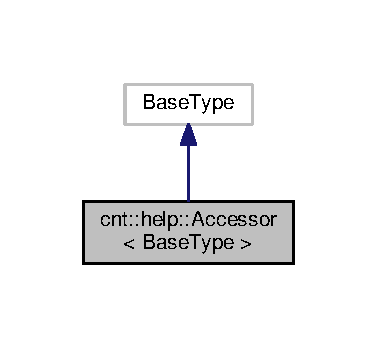
\includegraphics[width=181pt]{structcnt_1_1help_1_1Accessor__inherit__graph}
\end{center}
\end{figure}


Collaboration diagram for cnt\+:\+:help\+:\+:Accessor$<$ Base\+Type $>$\+:\nopagebreak
\begin{figure}[H]
\begin{center}
\leavevmode
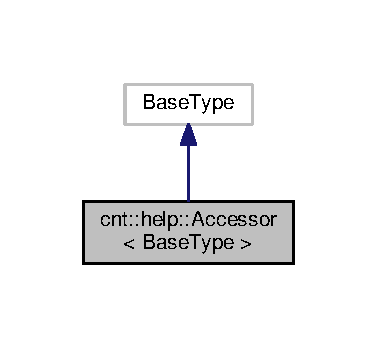
\includegraphics[width=181pt]{structcnt_1_1help_1_1Accessor__coll__graph}
\end{center}
\end{figure}
\subsection*{Public Types}
{\bf }\par
\begin{DoxyCompactItemize}
\item 
using \hyperlink{structcnt_1_1help_1_1Accessor_a6728450f8fdeca32e8ed372b41b3467b}{Base} = Base\+Type
\item 
using \hyperlink{structcnt_1_1help_1_1Accessor_ad8a10e7f904fd874307b32b298aa1d54}{value\+\_\+type} = typename Base\+::value\+\_\+type
\item 
using \hyperlink{structcnt_1_1help_1_1Accessor_a75659462be135d55bf8f4d6409b84a1f}{reference} = typename Base\+::reference
\item 
using \hyperlink{structcnt_1_1help_1_1Accessor_a8575d9de6bcb21a1bd6935d500cfcb89}{const\+\_\+reference} = typename Base\+::const\+\_\+reference
\end{DoxyCompactItemize}

\subsection*{Public Member Functions}
{\bf }\par
\begin{DoxyCompactItemize}
\item 
{\footnotesize template$<$typename... Args, Enable\+If\+Integral\+Or\+Iterable$<$ Args... $>$  = 0$>$ }\\\hyperlink{structcnt_1_1help_1_1Accessor_a8575d9de6bcb21a1bd6935d500cfcb89}{const\+\_\+reference} \hyperlink{structcnt_1_1help_1_1Accessor_afb70ea54cd8e9104c2767fd78984857d}{operator()} (const Args \&...args) const 
\begin{DoxyCompactList}\small\item\em Integral or Iterable types. \end{DoxyCompactList}\item 
{\footnotesize template$<$typename... Args, Enable\+If\+Integral\+Or\+Iterable$<$ Args... $>$  = 0$>$ }\\\hyperlink{structcnt_1_1help_1_1Accessor_a75659462be135d55bf8f4d6409b84a1f}{reference} \hyperlink{structcnt_1_1help_1_1Accessor_a30413bd6e851ed42d3ac78d839d6d45b}{operator()} (const Args \&...args)
\item 
{\footnotesize template$<$typename U , help\+::\+Enable\+If\+Iterator$<$ std\+::decay\+\_\+t$<$ U $>$$>$  = 0$>$ }\\\hyperlink{structcnt_1_1help_1_1Accessor_a8575d9de6bcb21a1bd6935d500cfcb89}{const\+\_\+reference} \hyperlink{structcnt_1_1help_1_1Accessor_a50f58d6227d262deddea121d510f393f}{operator()} (const U \&begin) const 
\begin{DoxyCompactList}\small\item\em Iterators. \end{DoxyCompactList}\item 
{\footnotesize template$<$typename U , help\+::\+Enable\+If\+Iterator$<$ std\+::decay\+\_\+t$<$ U $>$$>$  = 0$>$ }\\\hyperlink{structcnt_1_1help_1_1Accessor_a75659462be135d55bf8f4d6409b84a1f}{reference} \hyperlink{structcnt_1_1help_1_1Accessor_a4560af573dad5470885eac20b3fde6cb}{operator()} (const U \&begin)
\item 
{\footnotesize template$<$typename U , help\+::\+Enable\+If\+Integral$<$ std\+::decay\+\_\+t$<$ U $>$$>$  = 0$>$ }\\\hyperlink{structcnt_1_1help_1_1Accessor_a8575d9de6bcb21a1bd6935d500cfcb89}{const\+\_\+reference} \hyperlink{structcnt_1_1help_1_1Accessor_abb001ec4d22d578bd6d920bda29592b7}{operator()} ({\bf std\+::initializer\+\_\+list}$<$ U $>$ il) const 
\begin{DoxyCompactList}\small\item\em Specific for \textquotesingle{}{\bf std\+::initializer\+\_\+list}\textquotesingle{}. \end{DoxyCompactList}\item 
{\footnotesize template$<$typename U , help\+::\+Enable\+If\+Integral$<$ std\+::decay\+\_\+t$<$ U $>$ $>$  = 0$>$ }\\\hyperlink{structcnt_1_1help_1_1Accessor_a75659462be135d55bf8f4d6409b84a1f}{reference} \hyperlink{structcnt_1_1help_1_1Accessor_ad9d67b1bb8ab0a019e71e1a4d10739c7}{operator()} ({\bf std\+::initializer\+\_\+list}$<$ U $>$ il)
\item 
{\footnotesize template$<$typename... Args, help\+::\+Enable\+If\+Integral$<$ std\+::decay\+\_\+t$<$ Args $>$... $>$  = 0$>$ }\\constexpr \hyperlink{structcnt_1_1help_1_1Accessor_a8575d9de6bcb21a1bd6935d500cfcb89}{const\+\_\+reference} \hyperlink{structcnt_1_1help_1_1Accessor_adb43fbaf95d042436a2ec7c2b7d0d61e}{operator()} (const {\bf std\+::tuple}$<$ Args... $>$ \&tup) const 
\begin{DoxyCompactList}\small\item\em For tuples containing integrals or iterables. \end{DoxyCompactList}\item 
{\footnotesize template$<$typename... Args, help\+::\+Enable\+If\+Integral$<$ std\+::decay\+\_\+t$<$ Args $>$... $>$  = 0$>$ }\\constexpr \hyperlink{structcnt_1_1help_1_1Accessor_a75659462be135d55bf8f4d6409b84a1f}{reference} \hyperlink{structcnt_1_1help_1_1Accessor_abdfcf9908cd4fc0baa2fe3e4693f69a6}{operator()} (const {\bf std\+::tuple}$<$ Args... $>$ \&tup)
\item 
{\footnotesize template$<$typename... Args, std\+::size\+\_\+t... Js$>$ }\\constexpr \hyperlink{structcnt_1_1help_1_1Accessor_a8575d9de6bcb21a1bd6935d500cfcb89}{const\+\_\+reference} \hyperlink{structcnt_1_1help_1_1Accessor_a2e3bc15b7287554c474554e8085643d6}{operator()} (const {\bf std\+::tuple}$<$ Args... $>$ \&tup, std\+::index\+\_\+sequence$<$ Js... $>$) const 
\end{DoxyCompactItemize}



\subsection{Detailed Description}
\subsubsection*{template$<$class Base\+Type$>$\\*
struct cnt\+::help\+::\+Accessor$<$ Base\+Type $>$}

We inherit from either \textquotesingle{}\hyperlink{classcnt_1_1help_1_1Container}{Container}\textquotesingle{} or \textquotesingle{}\hyperlink{classcnt_1_1help_1_1Slice}{Slice}\textquotesingle{}. 

The only purpose of this class is to delegate calls to the accessors of \textquotesingle{}\hyperlink{classcnt_1_1help_1_1Container}{Container}\textquotesingle{} or \textquotesingle{}\hyperlink{classcnt_1_1help_1_1Slice}{Slice}\textquotesingle{}, so we dont have duplication of code and the classes can be written more clearly. 

\subsection{Member Typedef Documentation}
\index{cnt\+::help\+::\+Accessor@{cnt\+::help\+::\+Accessor}!Base@{Base}}
\index{Base@{Base}!cnt\+::help\+::\+Accessor@{cnt\+::help\+::\+Accessor}}
\subsubsection[{\texorpdfstring{Base}{Base}}]{\setlength{\rightskip}{0pt plus 5cm}template$<$class Base\+Type $>$ using {\bf cnt\+::help\+::\+Accessor}$<$ Base\+Type $>$\+::{\bf Base} =  Base\+Type}\hypertarget{structcnt_1_1help_1_1Accessor_a6728450f8fdeca32e8ed372b41b3467b}{}\label{structcnt_1_1help_1_1Accessor_a6728450f8fdeca32e8ed372b41b3467b}
Some type definitions \index{cnt\+::help\+::\+Accessor@{cnt\+::help\+::\+Accessor}!const\+\_\+reference@{const\+\_\+reference}}
\index{const\+\_\+reference@{const\+\_\+reference}!cnt\+::help\+::\+Accessor@{cnt\+::help\+::\+Accessor}}
\subsubsection[{\texorpdfstring{const\+\_\+reference}{const_reference}}]{\setlength{\rightskip}{0pt plus 5cm}template$<$class Base\+Type $>$ using {\bf cnt\+::help\+::\+Accessor}$<$ Base\+Type $>$\+::{\bf const\+\_\+reference} =  typename Base\+::const\+\_\+reference}\hypertarget{structcnt_1_1help_1_1Accessor_a8575d9de6bcb21a1bd6935d500cfcb89}{}\label{structcnt_1_1help_1_1Accessor_a8575d9de6bcb21a1bd6935d500cfcb89}
\index{cnt\+::help\+::\+Accessor@{cnt\+::help\+::\+Accessor}!reference@{reference}}
\index{reference@{reference}!cnt\+::help\+::\+Accessor@{cnt\+::help\+::\+Accessor}}
\subsubsection[{\texorpdfstring{reference}{reference}}]{\setlength{\rightskip}{0pt plus 5cm}template$<$class Base\+Type $>$ using {\bf cnt\+::help\+::\+Accessor}$<$ Base\+Type $>$\+::{\bf reference} =  typename Base\+::reference}\hypertarget{structcnt_1_1help_1_1Accessor_a75659462be135d55bf8f4d6409b84a1f}{}\label{structcnt_1_1help_1_1Accessor_a75659462be135d55bf8f4d6409b84a1f}
\index{cnt\+::help\+::\+Accessor@{cnt\+::help\+::\+Accessor}!value\+\_\+type@{value\+\_\+type}}
\index{value\+\_\+type@{value\+\_\+type}!cnt\+::help\+::\+Accessor@{cnt\+::help\+::\+Accessor}}
\subsubsection[{\texorpdfstring{value\+\_\+type}{value_type}}]{\setlength{\rightskip}{0pt plus 5cm}template$<$class Base\+Type $>$ using {\bf cnt\+::help\+::\+Accessor}$<$ Base\+Type $>$\+::{\bf value\+\_\+type} =  typename Base\+::value\+\_\+type}\hypertarget{structcnt_1_1help_1_1Accessor_ad8a10e7f904fd874307b32b298aa1d54}{}\label{structcnt_1_1help_1_1Accessor_ad8a10e7f904fd874307b32b298aa1d54}


\subsection{Member Function Documentation}
\index{cnt\+::help\+::\+Accessor@{cnt\+::help\+::\+Accessor}!operator()@{operator()}}
\index{operator()@{operator()}!cnt\+::help\+::\+Accessor@{cnt\+::help\+::\+Accessor}}
\subsubsection[{\texorpdfstring{operator()(const Args \&...\+args) const }{operator()(const Args &...args) const }}]{\setlength{\rightskip}{0pt plus 5cm}template$<$class Base\+Type $>$ template$<$typename... Args, Enable\+If\+Integral\+Or\+Iterable$<$ Args... $>$  = 0$>$ {\bf const\+\_\+reference} {\bf cnt\+::help\+::\+Accessor}$<$ Base\+Type $>$\+::operator() (
\begin{DoxyParamCaption}
\item[{const Args \&...}]{args}
\end{DoxyParamCaption}
) const\hspace{0.3cm}{\ttfamily [inline]}}\hypertarget{structcnt_1_1help_1_1Accessor_afb70ea54cd8e9104c2767fd78984857d}{}\label{structcnt_1_1help_1_1Accessor_afb70ea54cd8e9104c2767fd78984857d}


Integral or Iterable types. 

These functions simply delegate the access to either \textquotesingle{}\hyperlink{classcnt_1_1help_1_1Container}{Container}\textquotesingle{} or \textquotesingle{}\hyperlink{classcnt_1_1help_1_1Slice}{Slice}\textquotesingle{}, which have the same interface for access. They are also responsible to handle the S\+F\+I\+N\+AE to treat all different types of access. \index{cnt\+::help\+::\+Accessor@{cnt\+::help\+::\+Accessor}!operator()@{operator()}}
\index{operator()@{operator()}!cnt\+::help\+::\+Accessor@{cnt\+::help\+::\+Accessor}}
\subsubsection[{\texorpdfstring{operator()(const Args \&...\+args)}{operator()(const Args &...args)}}]{\setlength{\rightskip}{0pt plus 5cm}template$<$class Base\+Type $>$ template$<$typename... Args, Enable\+If\+Integral\+Or\+Iterable$<$ Args... $>$  = 0$>$ {\bf reference} {\bf cnt\+::help\+::\+Accessor}$<$ Base\+Type $>$\+::operator() (
\begin{DoxyParamCaption}
\item[{const Args \&...}]{args}
\end{DoxyParamCaption}
)\hspace{0.3cm}{\ttfamily [inline]}}\hypertarget{structcnt_1_1help_1_1Accessor_a30413bd6e851ed42d3ac78d839d6d45b}{}\label{structcnt_1_1help_1_1Accessor_a30413bd6e851ed42d3ac78d839d6d45b}
\index{cnt\+::help\+::\+Accessor@{cnt\+::help\+::\+Accessor}!operator()@{operator()}}
\index{operator()@{operator()}!cnt\+::help\+::\+Accessor@{cnt\+::help\+::\+Accessor}}
\subsubsection[{\texorpdfstring{operator()(const U \&begin) const }{operator()(const U &begin) const }}]{\setlength{\rightskip}{0pt plus 5cm}template$<$class Base\+Type $>$ template$<$typename U , help\+::\+Enable\+If\+Iterator$<$ std\+::decay\+\_\+t$<$ U $>$$>$  = 0$>$ {\bf const\+\_\+reference} {\bf cnt\+::help\+::\+Accessor}$<$ Base\+Type $>$\+::operator() (
\begin{DoxyParamCaption}
\item[{const U \&}]{begin}
\end{DoxyParamCaption}
) const\hspace{0.3cm}{\ttfamily [inline]}}\hypertarget{structcnt_1_1help_1_1Accessor_a50f58d6227d262deddea121d510f393f}{}\label{structcnt_1_1help_1_1Accessor_a50f58d6227d262deddea121d510f393f}


Iterators. 

\index{cnt\+::help\+::\+Accessor@{cnt\+::help\+::\+Accessor}!operator()@{operator()}}
\index{operator()@{operator()}!cnt\+::help\+::\+Accessor@{cnt\+::help\+::\+Accessor}}
\subsubsection[{\texorpdfstring{operator()(const U \&begin)}{operator()(const U &begin)}}]{\setlength{\rightskip}{0pt plus 5cm}template$<$class Base\+Type $>$ template$<$typename U , help\+::\+Enable\+If\+Iterator$<$ std\+::decay\+\_\+t$<$ U $>$$>$  = 0$>$ {\bf reference} {\bf cnt\+::help\+::\+Accessor}$<$ Base\+Type $>$\+::operator() (
\begin{DoxyParamCaption}
\item[{const U \&}]{begin}
\end{DoxyParamCaption}
)\hspace{0.3cm}{\ttfamily [inline]}}\hypertarget{structcnt_1_1help_1_1Accessor_a4560af573dad5470885eac20b3fde6cb}{}\label{structcnt_1_1help_1_1Accessor_a4560af573dad5470885eac20b3fde6cb}
\index{cnt\+::help\+::\+Accessor@{cnt\+::help\+::\+Accessor}!operator()@{operator()}}
\index{operator()@{operator()}!cnt\+::help\+::\+Accessor@{cnt\+::help\+::\+Accessor}}
\subsubsection[{\texorpdfstring{operator()(std\+::initializer\+\_\+list$<$ U $>$ il) const }{operator()(std::initializer_list< U > il) const }}]{\setlength{\rightskip}{0pt plus 5cm}template$<$class Base\+Type $>$ template$<$typename U , help\+::\+Enable\+If\+Integral$<$ std\+::decay\+\_\+t$<$ U $>$$>$  = 0$>$ {\bf const\+\_\+reference} {\bf cnt\+::help\+::\+Accessor}$<$ Base\+Type $>$\+::operator() (
\begin{DoxyParamCaption}
\item[{{\bf std\+::initializer\+\_\+list}$<$ U $>$}]{il}
\end{DoxyParamCaption}
) const\hspace{0.3cm}{\ttfamily [inline]}}\hypertarget{structcnt_1_1help_1_1Accessor_abb001ec4d22d578bd6d920bda29592b7}{}\label{structcnt_1_1help_1_1Accessor_abb001ec4d22d578bd6d920bda29592b7}


Specific for \textquotesingle{}{\bf std\+::initializer\+\_\+list}\textquotesingle{}. 

\index{cnt\+::help\+::\+Accessor@{cnt\+::help\+::\+Accessor}!operator()@{operator()}}
\index{operator()@{operator()}!cnt\+::help\+::\+Accessor@{cnt\+::help\+::\+Accessor}}
\subsubsection[{\texorpdfstring{operator()(std\+::initializer\+\_\+list$<$ U $>$ il)}{operator()(std::initializer_list< U > il)}}]{\setlength{\rightskip}{0pt plus 5cm}template$<$class Base\+Type $>$ template$<$typename U , help\+::\+Enable\+If\+Integral$<$ std\+::decay\+\_\+t$<$ U $>$ $>$  = 0$>$ {\bf reference} {\bf cnt\+::help\+::\+Accessor}$<$ Base\+Type $>$\+::operator() (
\begin{DoxyParamCaption}
\item[{{\bf std\+::initializer\+\_\+list}$<$ U $>$}]{il}
\end{DoxyParamCaption}
)\hspace{0.3cm}{\ttfamily [inline]}}\hypertarget{structcnt_1_1help_1_1Accessor_ad9d67b1bb8ab0a019e71e1a4d10739c7}{}\label{structcnt_1_1help_1_1Accessor_ad9d67b1bb8ab0a019e71e1a4d10739c7}
\index{cnt\+::help\+::\+Accessor@{cnt\+::help\+::\+Accessor}!operator()@{operator()}}
\index{operator()@{operator()}!cnt\+::help\+::\+Accessor@{cnt\+::help\+::\+Accessor}}
\subsubsection[{\texorpdfstring{operator()(const std\+::tuple$<$ Args... $>$ \&tup) const }{operator()(const std::tuple< Args... > &tup) const }}]{\setlength{\rightskip}{0pt plus 5cm}template$<$class Base\+Type $>$ template$<$typename... Args, help\+::\+Enable\+If\+Integral$<$ std\+::decay\+\_\+t$<$ Args $>$... $>$  = 0$>$ constexpr {\bf const\+\_\+reference} {\bf cnt\+::help\+::\+Accessor}$<$ Base\+Type $>$\+::operator() (
\begin{DoxyParamCaption}
\item[{const {\bf std\+::tuple}$<$ Args... $>$ \&}]{tup}
\end{DoxyParamCaption}
) const\hspace{0.3cm}{\ttfamily [inline]}}\hypertarget{structcnt_1_1help_1_1Accessor_adb43fbaf95d042436a2ec7c2b7d0d61e}{}\label{structcnt_1_1help_1_1Accessor_adb43fbaf95d042436a2ec7c2b7d0d61e}


For tuples containing integrals or iterables. 

\index{cnt\+::help\+::\+Accessor@{cnt\+::help\+::\+Accessor}!operator()@{operator()}}
\index{operator()@{operator()}!cnt\+::help\+::\+Accessor@{cnt\+::help\+::\+Accessor}}
\subsubsection[{\texorpdfstring{operator()(const std\+::tuple$<$ Args... $>$ \&tup)}{operator()(const std::tuple< Args... > &tup)}}]{\setlength{\rightskip}{0pt plus 5cm}template$<$class Base\+Type $>$ template$<$typename... Args, help\+::\+Enable\+If\+Integral$<$ std\+::decay\+\_\+t$<$ Args $>$... $>$  = 0$>$ constexpr {\bf reference} {\bf cnt\+::help\+::\+Accessor}$<$ Base\+Type $>$\+::operator() (
\begin{DoxyParamCaption}
\item[{const {\bf std\+::tuple}$<$ Args... $>$ \&}]{tup}
\end{DoxyParamCaption}
)\hspace{0.3cm}{\ttfamily [inline]}}\hypertarget{structcnt_1_1help_1_1Accessor_abdfcf9908cd4fc0baa2fe3e4693f69a6}{}\label{structcnt_1_1help_1_1Accessor_abdfcf9908cd4fc0baa2fe3e4693f69a6}
\index{cnt\+::help\+::\+Accessor@{cnt\+::help\+::\+Accessor}!operator()@{operator()}}
\index{operator()@{operator()}!cnt\+::help\+::\+Accessor@{cnt\+::help\+::\+Accessor}}
\subsubsection[{\texorpdfstring{operator()(const std\+::tuple$<$ Args... $>$ \&tup, std\+::index\+\_\+sequence$<$ Js... $>$) const }{operator()(const std::tuple< Args... > &tup, std::index_sequence< Js... >) const }}]{\setlength{\rightskip}{0pt plus 5cm}template$<$class Base\+Type $>$ template$<$typename... Args, std\+::size\+\_\+t... Js$>$ constexpr {\bf const\+\_\+reference} {\bf cnt\+::help\+::\+Accessor}$<$ Base\+Type $>$\+::operator() (
\begin{DoxyParamCaption}
\item[{const {\bf std\+::tuple}$<$ Args... $>$ \&}]{tup, }
\item[{std\+::index\+\_\+sequence$<$ Js... $>$}]{}
\end{DoxyParamCaption}
) const\hspace{0.3cm}{\ttfamily [inline]}}\hypertarget{structcnt_1_1help_1_1Accessor_a2e3bc15b7287554c474554e8085643d6}{}\label{structcnt_1_1help_1_1Accessor_a2e3bc15b7287554c474554e8085643d6}


The documentation for this struct was generated from the following file\+:\begin{DoxyCompactItemize}
\item 
/home/matheus/\+Algoritmos/\+C\+P\+P/\+Handy/include/\+Container/\hyperlink{Container_8h}{Container.\+h}\end{DoxyCompactItemize}

\hypertarget{structcnt_1_1help_1_1And}{}\section{cnt\+:\+:help\+:\+:And$<$... $>$ Struct Template Reference}
\label{structcnt_1_1help_1_1And}\index{cnt\+::help\+::\+And$<$... $>$@{cnt\+::help\+::\+And$<$... $>$}}


{\ttfamily \#include $<$Helpers.\+h$>$}



\subsection{Detailed Description}
\subsubsection*{template$<$bool...$>$\\*
struct cnt\+::help\+::\+And$<$... $>$}

Test truthness of variadic set of bool arguments. Only gives a true value if all elements are true. 

The documentation for this struct was generated from the following file\+:\begin{DoxyCompactItemize}
\item 
/home/matheus/\+Algoritmos/\+C\+P\+P/\+Handy/include/\+Container/\hyperlink{Container_2Helpers_8h}{Helpers.\+h}\end{DoxyCompactItemize}

\hypertarget{structhandy_1_1And}{}\section{handy\+:\+:And$<$... $>$ Struct Template Reference}
\label{structhandy_1_1And}\index{handy\+::\+And$<$... $>$@{handy\+::\+And$<$... $>$}}


Base definition.  




{\ttfamily \#include $<$Helpers.\+h$>$}



\subsection{Detailed Description}
\subsubsection*{template$<$bool...$>$\\*
struct handy\+::\+And$<$... $>$}

Base definition. 

The documentation for this struct was generated from the following file\+:\begin{DoxyCompactItemize}
\item 
/home/matheus/\+Algoritmos/\+C\+P\+P/\+Handy/include/\+Helpers/\hyperlink{Helpers_2Helpers_8h}{Helpers.\+h}\end{DoxyCompactItemize}

\hypertarget{structcnt_1_1help_1_1And_3_01B1_00_01Bs_8_8_8_01_4}{}\section{cnt\+:\+:help\+:\+:And$<$ B1, Bs... $>$ Struct Template Reference}
\label{structcnt_1_1help_1_1And_3_01B1_00_01Bs_8_8_8_01_4}\index{cnt\+::help\+::\+And$<$ B1, Bs... $>$@{cnt\+::help\+::\+And$<$ B1, Bs... $>$}}


{\ttfamily \#include $<$Helpers.\+h$>$}



Inheritance diagram for cnt\+:\+:help\+:\+:And$<$ B1, Bs... $>$\+:\nopagebreak
\begin{figure}[H]
\begin{center}
\leavevmode
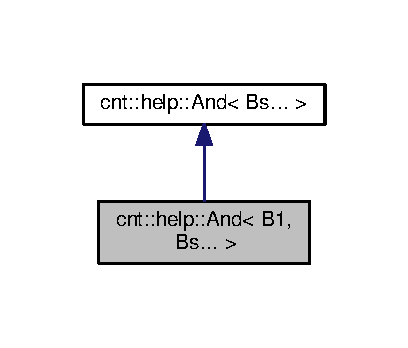
\includegraphics[width=196pt]{structcnt_1_1help_1_1And_3_01B1_00_01Bs_8_8_8_01_4__inherit__graph}
\end{center}
\end{figure}


Collaboration diagram for cnt\+:\+:help\+:\+:And$<$ B1, Bs... $>$\+:\nopagebreak
\begin{figure}[H]
\begin{center}
\leavevmode
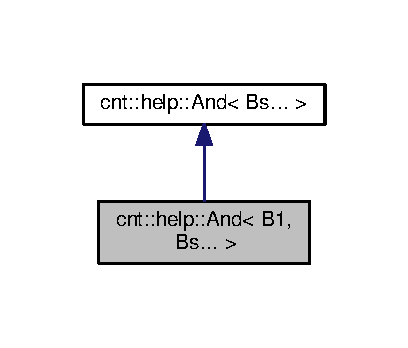
\includegraphics[width=196pt]{structcnt_1_1help_1_1And_3_01B1_00_01Bs_8_8_8_01_4__coll__graph}
\end{center}
\end{figure}


The documentation for this struct was generated from the following file\+:\begin{DoxyCompactItemize}
\item 
/home/matheus/\+Algoritmos/\+C\+P\+P/\+Handy/include/\+Container/\hyperlink{Container_2Helpers_8h}{Helpers.\+h}\end{DoxyCompactItemize}

\hypertarget{structhandy_1_1And_3_01B1_00_01Bs_8_8_8_01_4}{}\section{handy\+:\+:And$<$ B1, Bs... $>$ Struct Template Reference}
\label{structhandy_1_1And_3_01B1_00_01Bs_8_8_8_01_4}\index{handy\+::\+And$<$ B1, Bs... $>$@{handy\+::\+And$<$ B1, Bs... $>$}}


If {\ttfamily B1} is true, check for the rest.  




{\ttfamily \#include $<$Helpers.\+h$>$}



Inheritance diagram for handy\+:\+:And$<$ B1, Bs... $>$\+:\nopagebreak
\begin{figure}[H]
\begin{center}
\leavevmode
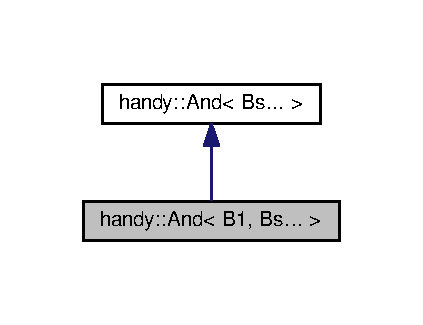
\includegraphics[width=203pt]{structhandy_1_1And_3_01B1_00_01Bs_8_8_8_01_4__inherit__graph}
\end{center}
\end{figure}


Collaboration diagram for handy\+:\+:And$<$ B1, Bs... $>$\+:\nopagebreak
\begin{figure}[H]
\begin{center}
\leavevmode
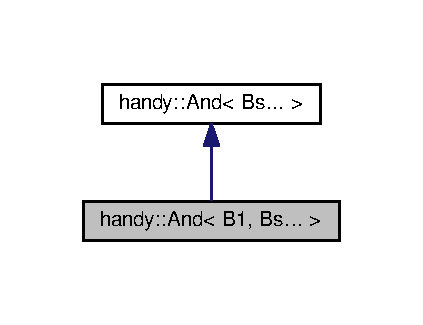
\includegraphics[width=203pt]{structhandy_1_1And_3_01B1_00_01Bs_8_8_8_01_4__coll__graph}
\end{center}
\end{figure}


\subsection{Detailed Description}
\subsubsection*{template$<$bool B1, bool... Bs$>$\\*
struct handy\+::\+And$<$ B1, Bs... $>$}

If {\ttfamily B1} is true, check for the rest. 

The documentation for this struct was generated from the following file\+:\begin{DoxyCompactItemize}
\item 
/home/matheus/\+Algoritmos/\+C\+P\+P/\+Handy/include/\+Helpers/\hyperlink{Helpers_2Helpers_8h}{Helpers.\+h}\end{DoxyCompactItemize}

\hypertarget{structcnt_1_1help_1_1And_3_01false_00_01Bs_8_8_8_01_4}{}\section{cnt\+:\+:help\+:\+:And$<$ false, Bs... $>$ Struct Template Reference}
\label{structcnt_1_1help_1_1And_3_01false_00_01Bs_8_8_8_01_4}\index{cnt\+::help\+::\+And$<$ false, Bs... $>$@{cnt\+::help\+::\+And$<$ false, Bs... $>$}}


{\ttfamily \#include $<$Helpers.\+h$>$}



Inheritance diagram for cnt\+:\+:help\+:\+:And$<$ false, Bs... $>$\+:\nopagebreak
\begin{figure}[H]
\begin{center}
\leavevmode
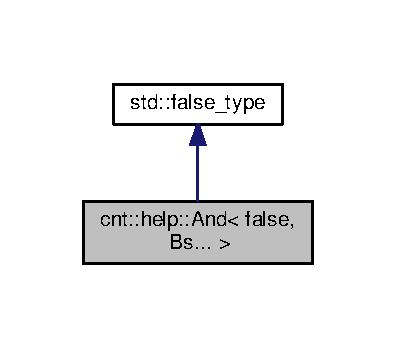
\includegraphics[width=190pt]{structcnt_1_1help_1_1And_3_01false_00_01Bs_8_8_8_01_4__inherit__graph}
\end{center}
\end{figure}


Collaboration diagram for cnt\+:\+:help\+:\+:And$<$ false, Bs... $>$\+:\nopagebreak
\begin{figure}[H]
\begin{center}
\leavevmode
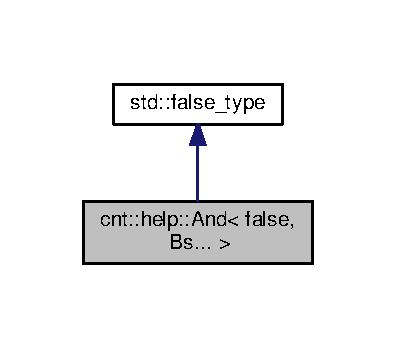
\includegraphics[width=190pt]{structcnt_1_1help_1_1And_3_01false_00_01Bs_8_8_8_01_4__coll__graph}
\end{center}
\end{figure}


The documentation for this struct was generated from the following file\+:\begin{DoxyCompactItemize}
\item 
/home/matheus/\+Algoritmos/\+C\+P\+P/\+Handy/include/\+Container/\hyperlink{Container_2Helpers_8h}{Helpers.\+h}\end{DoxyCompactItemize}

\hypertarget{structhandy_1_1And_3_01false_00_01Bs_8_8_8_01_4}{}\section{handy\+:\+:And$<$ false, Bs... $>$ Struct Template Reference}
\label{structhandy_1_1And_3_01false_00_01Bs_8_8_8_01_4}\index{handy\+::\+And$<$ false, Bs... $>$@{handy\+::\+And$<$ false, Bs... $>$}}


If the current argument ({\ttfamily B1}) is {\ttfamily false}, so the return can only be {\ttfamily false}.  




{\ttfamily \#include $<$Helpers.\+h$>$}



Inheritance diagram for handy\+:\+:And$<$ false, Bs... $>$\+:\nopagebreak
\begin{figure}[H]
\begin{center}
\leavevmode
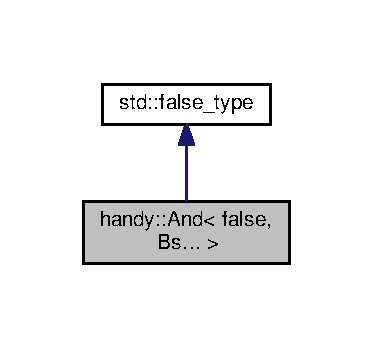
\includegraphics[width=179pt]{structhandy_1_1And_3_01false_00_01Bs_8_8_8_01_4__inherit__graph}
\end{center}
\end{figure}


Collaboration diagram for handy\+:\+:And$<$ false, Bs... $>$\+:\nopagebreak
\begin{figure}[H]
\begin{center}
\leavevmode
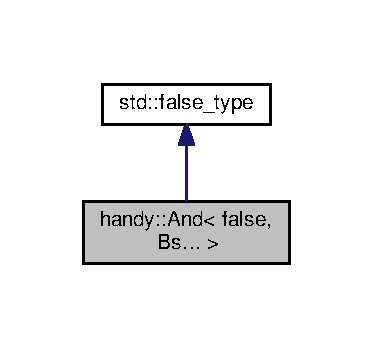
\includegraphics[width=179pt]{structhandy_1_1And_3_01false_00_01Bs_8_8_8_01_4__coll__graph}
\end{center}
\end{figure}


\subsection{Detailed Description}
\subsubsection*{template$<$bool... Bs$>$\\*
struct handy\+::\+And$<$ false, Bs... $>$}

If the current argument ({\ttfamily B1}) is {\ttfamily false}, so the return can only be {\ttfamily false}. 

The documentation for this struct was generated from the following file\+:\begin{DoxyCompactItemize}
\item 
/home/matheus/\+Algoritmos/\+C\+P\+P/\+Handy/include/\+Helpers/\hyperlink{Helpers_2Helpers_8h}{Helpers.\+h}\end{DoxyCompactItemize}

\hypertarget{structcnt_1_1help_1_1And_3_01true_01_4}{}\section{cnt\+:\+:help\+:\+:And$<$ true $>$ Struct Template Reference}
\label{structcnt_1_1help_1_1And_3_01true_01_4}\index{cnt\+::help\+::\+And$<$ true $>$@{cnt\+::help\+::\+And$<$ true $>$}}


{\ttfamily \#include $<$Helpers.\+h$>$}



Inheritance diagram for cnt\+:\+:help\+:\+:And$<$ true $>$\+:\nopagebreak
\begin{figure}[H]
\begin{center}
\leavevmode
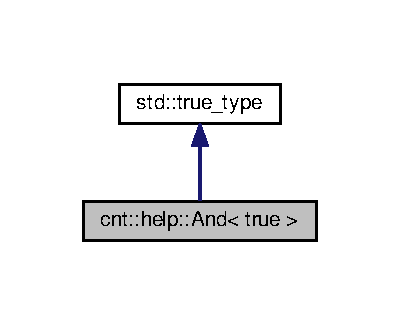
\includegraphics[width=192pt]{structcnt_1_1help_1_1And_3_01true_01_4__inherit__graph}
\end{center}
\end{figure}


Collaboration diagram for cnt\+:\+:help\+:\+:And$<$ true $>$\+:\nopagebreak
\begin{figure}[H]
\begin{center}
\leavevmode
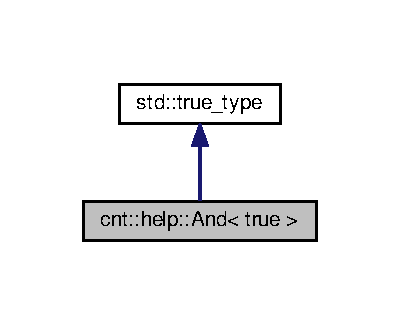
\includegraphics[width=192pt]{structcnt_1_1help_1_1And_3_01true_01_4__coll__graph}
\end{center}
\end{figure}


The documentation for this struct was generated from the following file\+:\begin{DoxyCompactItemize}
\item 
/home/matheus/\+Algoritmos/\+C\+P\+P/\+Handy/include/\+Container/\hyperlink{Container_2Helpers_8h}{Helpers.\+h}\end{DoxyCompactItemize}

\hypertarget{structcnt_1_1help_1_1And_3_4}{}\section{cnt\+:\+:help\+:\+:And$<$$>$ Struct Template Reference}
\label{structcnt_1_1help_1_1And_3_4}\index{cnt\+::help\+::\+And$<$$>$@{cnt\+::help\+::\+And$<$$>$}}


{\ttfamily \#include $<$Helpers.\+h$>$}



Inheritance diagram for cnt\+:\+:help\+:\+:And$<$$>$\+:\nopagebreak
\begin{figure}[H]
\begin{center}
\leavevmode
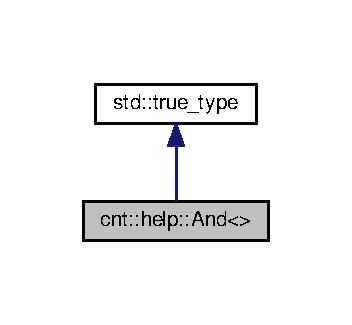
\includegraphics[width=169pt]{structcnt_1_1help_1_1And_3_4__inherit__graph}
\end{center}
\end{figure}


Collaboration diagram for cnt\+:\+:help\+:\+:And$<$$>$\+:\nopagebreak
\begin{figure}[H]
\begin{center}
\leavevmode
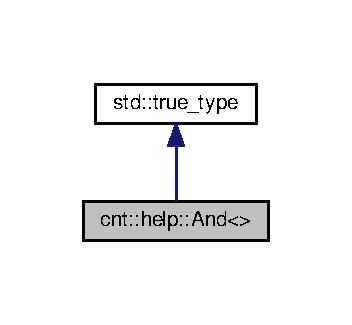
\includegraphics[width=169pt]{structcnt_1_1help_1_1And_3_4__coll__graph}
\end{center}
\end{figure}


The documentation for this struct was generated from the following file\+:\begin{DoxyCompactItemize}
\item 
/home/matheus/\+Algoritmos/\+C\+P\+P/\+Handy/include/\+Container/\hyperlink{Container_2Helpers_8h}{Helpers.\+h}\end{DoxyCompactItemize}

\hypertarget{structhandy_1_1And_3_4}{}\section{handy\+:\+:And$<$$>$ Struct Template Reference}
\label{structhandy_1_1And_3_4}\index{handy\+::\+And$<$$>$@{handy\+::\+And$<$$>$}}


If none of the arguments are {\ttfamily false}, so the result is {\ttfamily true}.  




{\ttfamily \#include $<$Helpers.\+h$>$}



Inheritance diagram for handy\+:\+:And$<$$>$\+:\nopagebreak
\begin{figure}[H]
\begin{center}
\leavevmode
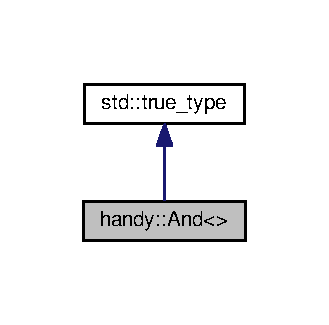
\includegraphics[width=158pt]{structhandy_1_1And_3_4__inherit__graph}
\end{center}
\end{figure}


Collaboration diagram for handy\+:\+:And$<$$>$\+:\nopagebreak
\begin{figure}[H]
\begin{center}
\leavevmode
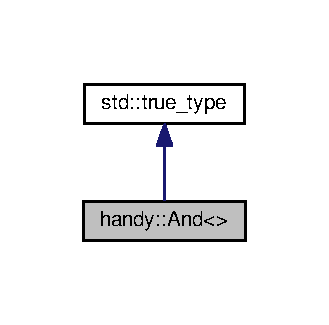
\includegraphics[width=158pt]{structhandy_1_1And_3_4__coll__graph}
\end{center}
\end{figure}


\subsection{Detailed Description}
\subsubsection*{template$<$$>$\\*
struct handy\+::\+And$<$$>$}

If none of the arguments are {\ttfamily false}, so the result is {\ttfamily true}. 

The documentation for this struct was generated from the following file\+:\begin{DoxyCompactItemize}
\item 
/home/matheus/\+Algoritmos/\+C\+P\+P/\+Handy/include/\+Helpers/\hyperlink{Helpers_2Helpers_8h}{Helpers.\+h}\end{DoxyCompactItemize}

\hypertarget{classhandy_1_1impl_1_1Benchmark}{}\section{handy\+:\+:impl\+:\+:Benchmark$<$ Start\+On\+Creation $>$ Class Template Reference}
\label{classhandy_1_1impl_1_1Benchmark}\index{handy\+::impl\+::\+Benchmark$<$ Start\+On\+Creation $>$@{handy\+::impl\+::\+Benchmark$<$ Start\+On\+Creation $>$}}


A class to do precise benchmarking on both Windows and Linux.  




{\ttfamily \#include $<$Benchmark.\+h$>$}

\subsection*{Public Member Functions}
\begin{DoxyCompactItemize}
\item 
{\footnotesize template$<$bool B = Start\+On\+Creation, typename std\+::enable\+\_\+if$<$ B $>$\+::type $\ast$  = nullptr$>$ }\\\hyperlink{group__BenchmarkGroup_ga1ba032700225aabb43579c633d7838b1}{Benchmark} ()
\begin{DoxyCompactList}\small\item\em Call the start function on creation if {\ttfamily Start\+On\+Creation} is {\ttfamily true}. \end{DoxyCompactList}\item 
{\footnotesize template$<$bool B = Start\+On\+Creation, typename std\+::enable\+\_\+if$<$!\+B $>$\+::type $\ast$  = nullptr$>$ }\\\hyperlink{classhandy_1_1impl_1_1Benchmark_ga1ba032700225aabb43579c633d7838b1}{Benchmark} ()
\begin{DoxyCompactList}\small\item\em Do nothing if {\ttfamily Start\+On\+Creation} is {\ttfamily false}. \end{DoxyCompactList}\item 
{\footnotesize template$<$class F , typename... Args$>$ }\\double \hyperlink{group__BenchmarkGroup_ga5eee042d87e75a24021ad6851a2c10ec}{operator()} (F \&\&f, Args \&\&...args)
\begin{DoxyCompactList}\small\item\em You can also use this operator and pass a function along with its arguments. \end{DoxyCompactList}\item 
void \hyperlink{group__BenchmarkGroup_gac7a583bb5a04f8028b8cc71a7db8fe80}{start} ()
\begin{DoxyCompactList}\small\item\em Start clock. \end{DoxyCompactList}\item 
double \hyperlink{group__BenchmarkGroup_ga1d7b23a0eeb6280431e0265cbdac1962}{finish} ()
\begin{DoxyCompactList}\small\item\em Stop clock and return time elapsed. \end{DoxyCompactList}\end{DoxyCompactItemize}


\subsection{Detailed Description}
\subsubsection*{template$<$bool Start\+On\+Creation = true$>$\\*
class handy\+::impl\+::\+Benchmark$<$ Start\+On\+Creation $>$}

A class to do precise benchmarking on both Windows and Linux. 


\begin{DoxyTemplParams}{Template Parameters}
{\em Start\+On\+Creation} & {\ttfamily bool} template constant telling if the clock initialization must be done at creation\\
\hline
\end{DoxyTemplParams}
If {\ttfamily Start\+On\+Creation} is {\ttfamily true}, this class initializes the clock on creation. You can also reset it by calling the \hyperlink{group__BenchmarkGroup_gac7a583bb5a04f8028b8cc71a7db8fe80}{start()} function. The \hyperlink{group__BenchmarkGroup_ga1d7b23a0eeb6280431e0265cbdac1962}{finish()} function returns the time (in seconds, up to nanoseconds of precision) elapsed since the call to the \hyperlink{group__BenchmarkGroup_gac7a583bb5a04f8028b8cc71a7db8fe80}{start()} function. 

\subsection{Constructor \& Destructor Documentation}
\index{handy\+::impl\+::\+Benchmark@{handy\+::impl\+::\+Benchmark}!Benchmark@{Benchmark}}
\index{Benchmark@{Benchmark}!handy\+::impl\+::\+Benchmark@{handy\+::impl\+::\+Benchmark}}
\subsubsection[{\texorpdfstring{Benchmark()}{Benchmark()}}]{\setlength{\rightskip}{0pt plus 5cm}template$<$bool Start\+On\+Creation = true$>$ template$<$bool B = Start\+On\+Creation, typename std\+::enable\+\_\+if$<$!\+B $>$\+::type $\ast$  = nullptr$>$ {\bf handy\+::impl\+::\+Benchmark}$<$ Start\+On\+Creation $>$\+::{\bf Benchmark} (
\begin{DoxyParamCaption}
{}
\end{DoxyParamCaption}
)\hspace{0.3cm}{\ttfamily [inline]}}\hypertarget{classhandy_1_1impl_1_1Benchmark_ga1ba032700225aabb43579c633d7838b1}{}\label{classhandy_1_1impl_1_1Benchmark_ga1ba032700225aabb43579c633d7838b1}


Do nothing if {\ttfamily Start\+On\+Creation} is {\ttfamily false}. 



The documentation for this class was generated from the following file\+:\begin{DoxyCompactItemize}
\item 
/home/matheus/\+Algoritmos/\+C\+P\+P/\+Handy/include/\+Helpers/\hyperlink{Benchmark_8h}{Benchmark.\+h}\end{DoxyCompactItemize}

\hypertarget{structhandy_1_1impl_1_1ClosedInterval}{}\section{handy\+:\+:impl\+:\+:Closed\+Interval Struct Reference}
\label{structhandy_1_1impl_1_1ClosedInterval}\index{handy\+::impl\+::\+Closed\+Interval@{handy\+::impl\+::\+Closed\+Interval}}


{\ttfamily \#include $<$Range.\+h$>$}

\subsection*{Public Member Functions}
\begin{DoxyCompactItemize}
\item 
{\footnotesize template$<$typename T $>$ }\\bool \hyperlink{structhandy_1_1impl_1_1ClosedInterval_a1714acc5bcb1aed7c66a3542b2ab395a}{operator()} (const T \&first, const T \&last, const T \&step) const 
\end{DoxyCompactItemize}


\subsection{Member Function Documentation}
\index{handy\+::impl\+::\+Closed\+Interval@{handy\+::impl\+::\+Closed\+Interval}!operator()@{operator()}}
\index{operator()@{operator()}!handy\+::impl\+::\+Closed\+Interval@{handy\+::impl\+::\+Closed\+Interval}}
\subsubsection[{\texorpdfstring{operator()(const T \&first, const T \&last, const T \&step) const }{operator()(const T &first, const T &last, const T &step) const }}]{\setlength{\rightskip}{0pt plus 5cm}template$<$typename T $>$ bool handy\+::impl\+::\+Closed\+Interval\+::operator() (
\begin{DoxyParamCaption}
\item[{const T \&}]{first, }
\item[{const T \&}]{last, }
\item[{const T \&}]{step}
\end{DoxyParamCaption}
) const\hspace{0.3cm}{\ttfamily [inline]}}\hypertarget{structhandy_1_1impl_1_1ClosedInterval_a1714acc5bcb1aed7c66a3542b2ab395a}{}\label{structhandy_1_1impl_1_1ClosedInterval_a1714acc5bcb1aed7c66a3542b2ab395a}


The documentation for this struct was generated from the following file\+:\begin{DoxyCompactItemize}
\item 
/home/matheus/\+Algoritmos/\+C\+P\+P/\+Handy/include/\+Range/\hyperlink{Range_8h}{Range.\+h}\end{DoxyCompactItemize}

\hypertarget{classcnt_1_1help_1_1Container}{}\section{cnt\+:\+:help\+:\+:Container$<$ T, Is $>$ Class Template Reference}
\label{classcnt_1_1help_1_1Container}\index{cnt\+::help\+::\+Container$<$ T, Is $>$@{cnt\+::help\+::\+Container$<$ T, Is $>$}}


{\ttfamily \#include $<$Container.\+h$>$}



Inheritance diagram for cnt\+:\+:help\+:\+:Container$<$ T, Is $>$\+:\nopagebreak
\begin{figure}[H]
\begin{center}
\leavevmode
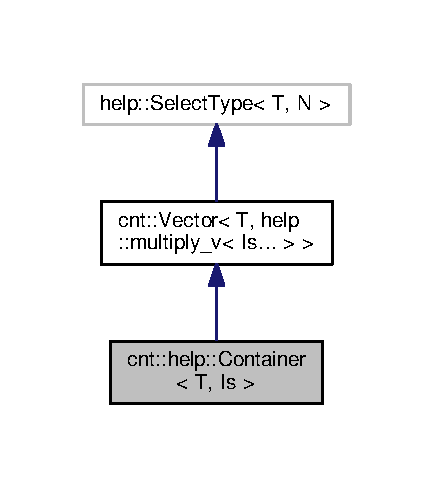
\includegraphics[width=208pt]{classcnt_1_1help_1_1Container__inherit__graph}
\end{center}
\end{figure}


Collaboration diagram for cnt\+:\+:help\+:\+:Container$<$ T, Is $>$\+:\nopagebreak
\begin{figure}[H]
\begin{center}
\leavevmode
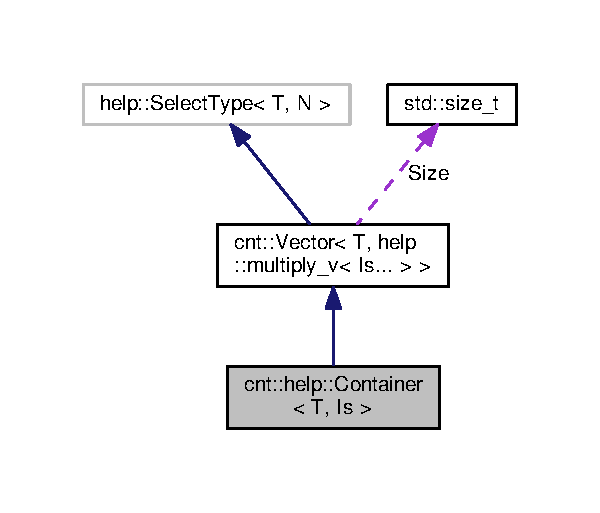
\includegraphics[width=288pt]{classcnt_1_1help_1_1Container__coll__graph}
\end{center}
\end{figure}
\subsection*{Public Types}
{\bf }\par
\begin{DoxyCompactItemize}
\item 
using \hyperlink{classcnt_1_1help_1_1Container_a0996cbe40d133dbec82facc6a17cf1f8}{Base} = \hyperlink{structcnt_1_1Vector}{Vector}$<$ T, \hyperlink{namespacecnt_1_1help_ab018f6aa5c1016ecf5d0d825cf8d362f}{help\+::multiply\+\_\+v}$<$ Is... $>$$>$
\item 
using \hyperlink{classcnt_1_1help_1_1Container_ada2fa1912d0bac79c0c631fe9a804027}{value\+\_\+type} = typename Base\+::value\+\_\+type
\item 
using \hyperlink{classcnt_1_1help_1_1Container_a11ea1092d03b288fe285601e98f7236c}{reference} = typename Base\+::reference
\item 
using \hyperlink{classcnt_1_1help_1_1Container_a388ebfcebe3759453a569af7d57267b5}{const\+\_\+reference} = typename Base\+::const\+\_\+reference
\end{DoxyCompactItemize}

\subsection*{Public Member Functions}
\begin{DoxyCompactItemize}
\item 
{\footnotesize template$<$typename... Args, std\+::size\+\_\+t M = Size, help\+::\+Enable\+If\+Array$<$ M $>$  = 0$>$ }\\\hyperlink{classcnt_1_1help_1_1Container_aed351dd256e42cc3c4976cf8fba1ccc4}{Container} (Args \&\&...args)
\begin{DoxyCompactList}\small\item\em Friend definition for the \textquotesingle{}\hyperlink{classcnt_1_1help_1_1Slice}{Slice}\textquotesingle{} class. \end{DoxyCompactList}\item 
{\footnotesize template$<$typename... Args, std\+::size\+\_\+t M = Size, std\+::enable\+\_\+if\+\_\+t$<$(\+M $>$  = help\+::max\+Size$>$ }\\\hyperlink{classcnt_1_1help_1_1Container_aed351dd256e42cc3c4976cf8fba1ccc4}{Container} (Args \&\&...args)
\item 
{\footnotesize template$<$std\+::size\+\_\+t M = Size, help\+::\+Enable\+If\+Zero$<$ M $>$  = 0$>$ }\\\hyperlink{classcnt_1_1help_1_1Container_a6f9ad3c670794e4e87a53f7bfe5557bb}{Container} ()
\begin{DoxyCompactList}\small\item\em Empty constructor for the case where \textquotesingle{}Size\textquotesingle{} is 0 (no compile time size is given) \end{DoxyCompactList}\item 
{\footnotesize template$<$typename... Args, std\+::size\+\_\+t M = Size, help\+::\+Enable\+If\+Zero$<$ M $>$  = 0, help\+::\+Enable\+If\+Integral$<$ std\+::decay\+\_\+t$<$ Args $>$... $>$  = 0$>$ }\\\hyperlink{classcnt_1_1help_1_1Container_a71204ac9d606898107ab40c90ff6632d}{Container} (Args...\+args)
\item 
{\footnotesize template$<$class... Args, std\+::size\+\_\+t M = Size, help\+::\+Enable\+If\+Zero$<$ M $>$  = 0, help\+::\+Enable\+If\+Iterable$<$ std\+::remove\+\_\+reference\+\_\+t$<$ Args $>$... $>$  = 0$>$ }\\\hyperlink{classcnt_1_1help_1_1Container_aa199ac743a8e601ca03a594f2da3d04d}{Container} (const Args \&...args)
\item 
{\footnotesize template$<$typename U , typename V , std\+::size\+\_\+t M = Size, help\+::\+Enable\+If\+Zero$<$ M $>$  = 0, help\+::\+Enable\+If\+Iterator$<$ std\+::decay\+\_\+t$<$ U $>$, std\+::decay\+\_\+t$<$ V $>$ $>$  = 0$>$ }\\\hyperlink{classcnt_1_1help_1_1Container_a7f6bc5fa04c8d13035afa70451f284ba}{Container} (const U \&begin, const V \&end)
\item 
{\footnotesize template$<$typename U , std\+::size\+\_\+t M = Size, help\+::\+Enable\+If\+Zero$<$ M $>$  = 0, help\+::\+Enable\+If\+Integral$<$ std\+::decay\+\_\+t$<$ U $>$$>$  = 0$>$ }\\\hyperlink{classcnt_1_1help_1_1Container_ae224bd9d879e6d4a64c5c8012f37e118}{Container} ({\bf std\+::initializer\+\_\+list}$<$ U $>$ il)
\item 
void \hyperlink{classcnt_1_1help_1_1Container_abf2fe8cb94e2f888a13a3012326aa85e}{init\+Weights} ()
\item 
constexpr {\bf std\+::size\+\_\+t} \hyperlink{classcnt_1_1help_1_1Container_a90bd1c3efe449d1f05ac28c443f0b8d8}{size} (int p) const 
\begin{DoxyCompactList}\small\item\em Size of each dimension. \end{DoxyCompactList}\item 
constexpr {\bf std\+::size\+\_\+t} \hyperlink{classcnt_1_1help_1_1Container_a02a5c3d38936e4b929e20fa367600495}{size} () const 
\begin{DoxyCompactList}\small\item\em Total size. \end{DoxyCompactList}\item 
constexpr auto \hyperlink{classcnt_1_1help_1_1Container_a08be97b830ab4e6fa1f619c6be405681}{sizes} () const 
\item 
constexpr {\bf std\+::size\+\_\+t} \hyperlink{classcnt_1_1help_1_1Container_a59a40323af244d48fd2dabf2d3b1313a}{num\+Dimensions} () const 
\end{DoxyCompactItemize}
{\bf }\par
\begin{DoxyCompactItemize}
\item 
{\footnotesize template$<$typename... Args$>$ }\\\hyperlink{classcnt_1_1help_1_1Container_a388ebfcebe3759453a569af7d57267b5}{const\+\_\+reference} \hyperlink{classcnt_1_1help_1_1Container_a3f9e15cd0863d4f954b5d5e810913866}{operator()} (\hyperlink{structcnt_1_1help_1_1IntegralType}{Integral\+Type}, const Args \&...args) const 
\item 
{\footnotesize template$<$typename U $>$ }\\\hyperlink{classcnt_1_1help_1_1Container_a388ebfcebe3759453a569af7d57267b5}{const\+\_\+reference} \hyperlink{classcnt_1_1help_1_1Container_ac0bfad14c0d0fe9ab0d8cf61530ea5e9}{operator()} (\hyperlink{structcnt_1_1help_1_1IteratorType}{Iterator\+Type}, const U \&begin) const 
\end{DoxyCompactItemize}

{\bf }\par
\begin{DoxyCompactItemize}
\item 
{\footnotesize template$<$typename U $>$ }\\\hyperlink{classcnt_1_1help_1_1Container_a388ebfcebe3759453a569af7d57267b5}{const\+\_\+reference} \hyperlink{classcnt_1_1help_1_1Container_a4917f3fa40a032a993114b423b6f6676}{operator()} ({\bf std\+::initializer\+\_\+list}$<$ U $>$ il) const 
\end{DoxyCompactItemize}

{\bf }\par
\begin{DoxyCompactItemize}
\item 
{\footnotesize template$<$typename... Args$>$ }\\auto \hyperlink{classcnt_1_1help_1_1Container_a800ac21ca3d9d89becb0a532cf3c5c08}{slice} (const Args \&...args) const 
\item 
{\footnotesize template$<$typename... Args$>$ }\\auto \hyperlink{classcnt_1_1help_1_1Container_aa465cba47315d064aeae1048e6547445}{slice} (const Args \&...args)
\end{DoxyCompactItemize}

\subsection*{Static Public Member Functions}
\begin{DoxyCompactItemize}
\item 
{\footnotesize template$<$typename U , typename Iter , help\+::\+Enable\+If\+Integral$<$ std\+::decay\+\_\+t$<$ U $>$$>$  = 0$>$ }\\static {\bf std\+::size\+\_\+t} \hyperlink{classcnt_1_1help_1_1Container_a4a4953ce456208660cdbc8dfbc8eb50e}{increment} (U u, Iter \&iter)
\item 
{\footnotesize template$<$typename U , typename Iter , help\+::\+Enable\+If\+Iterable$<$ std\+::decay\+\_\+t$<$ U $>$$>$  = 0$>$ }\\static {\bf std\+::size\+\_\+t} \hyperlink{classcnt_1_1help_1_1Container_a7fe8455c16cc35c3f30c00151f332dfc}{increment} (const U \&u, Iter \&iter)
\end{DoxyCompactItemize}
\subsection*{Friends}
\begin{DoxyCompactItemize}
\item 
class \hyperlink{classcnt_1_1help_1_1Container_aebd52b76fc246e48b629887d4025eda6}{Slice$<$ Container $>$}
\item 
class \hyperlink{classcnt_1_1help_1_1Container_aa082f0b2bccdce6fc9fc7339bf98a2b1}{Slice$<$ const Container $>$}
\begin{DoxyCompactList}\small\item\em Friend definition for the \textquotesingle{}\hyperlink{classcnt_1_1help_1_1Slice}{Slice}\textquotesingle{} class. \end{DoxyCompactList}\end{DoxyCompactItemize}
\subsection*{Additional Inherited Members}


\subsection{Detailed Description}
\subsubsection*{template$<$typename T, std\+::size\+\_\+t... Is$>$\\*
class cnt\+::help\+::\+Container$<$ T, Is $>$}

Class to easily create and manipulate multidimensional data. Interacts easily with S\+TL algorithms and can be either statically or dinamically allocated.


\begin{DoxyTemplParams}{Template Parameters}
{\em T} & The Containers type \\
\hline
{\em Is} & The compile time size of each dimension. The total size is the multiplication of these sizes. See the \textquotesingle{}\hyperlink{structcnt_1_1Vector}{Vector}\textquotesingle{} class. \\
\hline
\end{DoxyTemplParams}


\subsection{Member Typedef Documentation}
\index{cnt\+::help\+::\+Container@{cnt\+::help\+::\+Container}!Base@{Base}}
\index{Base@{Base}!cnt\+::help\+::\+Container@{cnt\+::help\+::\+Container}}
\subsubsection[{\texorpdfstring{Base}{Base}}]{\setlength{\rightskip}{0pt plus 5cm}template$<$typename T , std\+::size\+\_\+t... Is$>$ using {\bf cnt\+::help\+::\+Container}$<$ T, Is $>$\+::{\bf Base} =  {\bf Vector}$<$T, {\bf help\+::multiply\+\_\+v}$<$Is...$>$$>$}\hypertarget{classcnt_1_1help_1_1Container_a0996cbe40d133dbec82facc6a17cf1f8}{}\label{classcnt_1_1help_1_1Container_a0996cbe40d133dbec82facc6a17cf1f8}
Some type definitions \index{cnt\+::help\+::\+Container@{cnt\+::help\+::\+Container}!const\+\_\+reference@{const\+\_\+reference}}
\index{const\+\_\+reference@{const\+\_\+reference}!cnt\+::help\+::\+Container@{cnt\+::help\+::\+Container}}
\subsubsection[{\texorpdfstring{const\+\_\+reference}{const_reference}}]{\setlength{\rightskip}{0pt plus 5cm}template$<$typename T , std\+::size\+\_\+t... Is$>$ using {\bf cnt\+::help\+::\+Container}$<$ T, Is $>$\+::{\bf const\+\_\+reference} =  typename Base\+::const\+\_\+reference}\hypertarget{classcnt_1_1help_1_1Container_a388ebfcebe3759453a569af7d57267b5}{}\label{classcnt_1_1help_1_1Container_a388ebfcebe3759453a569af7d57267b5}
\index{cnt\+::help\+::\+Container@{cnt\+::help\+::\+Container}!reference@{reference}}
\index{reference@{reference}!cnt\+::help\+::\+Container@{cnt\+::help\+::\+Container}}
\subsubsection[{\texorpdfstring{reference}{reference}}]{\setlength{\rightskip}{0pt plus 5cm}template$<$typename T , std\+::size\+\_\+t... Is$>$ using {\bf cnt\+::help\+::\+Container}$<$ T, Is $>$\+::{\bf reference} =  typename Base\+::reference}\hypertarget{classcnt_1_1help_1_1Container_a11ea1092d03b288fe285601e98f7236c}{}\label{classcnt_1_1help_1_1Container_a11ea1092d03b288fe285601e98f7236c}
\index{cnt\+::help\+::\+Container@{cnt\+::help\+::\+Container}!value\+\_\+type@{value\+\_\+type}}
\index{value\+\_\+type@{value\+\_\+type}!cnt\+::help\+::\+Container@{cnt\+::help\+::\+Container}}
\subsubsection[{\texorpdfstring{value\+\_\+type}{value_type}}]{\setlength{\rightskip}{0pt plus 5cm}template$<$typename T , std\+::size\+\_\+t... Is$>$ using {\bf cnt\+::help\+::\+Container}$<$ T, Is $>$\+::{\bf value\+\_\+type} =  typename Base\+::value\+\_\+type}\hypertarget{classcnt_1_1help_1_1Container_ada2fa1912d0bac79c0c631fe9a804027}{}\label{classcnt_1_1help_1_1Container_ada2fa1912d0bac79c0c631fe9a804027}


\subsection{Constructor \& Destructor Documentation}
\index{cnt\+::help\+::\+Container@{cnt\+::help\+::\+Container}!Container@{Container}}
\index{Container@{Container}!cnt\+::help\+::\+Container@{cnt\+::help\+::\+Container}}
\subsubsection[{\texorpdfstring{Container(\+Args \&\&...\+args)}{Container(Args &&...args)}}]{\setlength{\rightskip}{0pt plus 5cm}template$<$typename T , std\+::size\+\_\+t... Is$>$ template$<$typename... Args, std\+::size\+\_\+t M = Size, help\+::\+Enable\+If\+Array$<$ M $>$  = 0$>$ {\bf cnt\+::help\+::\+Container}$<$ T, Is $>$\+::{\bf Container} (
\begin{DoxyParamCaption}
\item[{Args \&\&...}]{args}
\end{DoxyParamCaption}
)\hspace{0.3cm}{\ttfamily [inline]}}\hypertarget{classcnt_1_1help_1_1Container_aed351dd256e42cc3c4976cf8fba1ccc4}{}\label{classcnt_1_1help_1_1Container_aed351dd256e42cc3c4976cf8fba1ccc4}


Friend definition for the \textquotesingle{}\hyperlink{classcnt_1_1help_1_1Slice}{Slice}\textquotesingle{} class. 

Constructor defined when inheriting from \textquotesingle{}{\bf std\+::array}\textquotesingle{}. Simulates \textquotesingle{}{\bf std\+::array}\textquotesingle{} list initialization. The number of dimensions is given by \textquotesingle{}Is\textquotesingle{}.

\mbox{[}in\mbox{]} args Variadic arguments. \textquotesingle{}\hyperlink{structcnt_1_1Vector}{Vector}\textquotesingle{} checks if they are of type \textquotesingle{}T\textquotesingle{}. \index{cnt\+::help\+::\+Container@{cnt\+::help\+::\+Container}!Container@{Container}}
\index{Container@{Container}!cnt\+::help\+::\+Container@{cnt\+::help\+::\+Container}}
\subsubsection[{\texorpdfstring{Container(\+Args \&\&...\+args)}{Container(Args &&...args)}}]{\setlength{\rightskip}{0pt plus 5cm}template$<$typename T , std\+::size\+\_\+t... Is$>$ template$<$typename... Args, std\+::size\+\_\+t M = Size, std\+::enable\+\_\+if\+\_\+t$<$(\+M $>$  = help\+::max\+Size$>$ {\bf cnt\+::help\+::\+Container}$<$ T, Is $>$\+::{\bf Container} (
\begin{DoxyParamCaption}
\item[{Args \&\&...}]{args}
\end{DoxyParamCaption}
)\hspace{0.3cm}{\ttfamily [inline]}}\hypertarget{classcnt_1_1help_1_1Container_aed351dd256e42cc3c4976cf8fba1ccc4}{}\label{classcnt_1_1help_1_1Container_aed351dd256e42cc3c4976cf8fba1ccc4}
Same as above, but now for a \textquotesingle{}\hyperlink{classcnt_1_1help_1_1Container}{Container}\textquotesingle{} inheriting from \textquotesingle{}{\bf std\+::vector}\textquotesingle{} with \textquotesingle{}Size\textquotesingle{} greater than the maximum stack allocation size. In this case, we must resize to \textquotesingle{}Size\textquotesingle{} after intiallizing with \textquotesingle{}args\textquotesingle{}.

\mbox{[}in\mbox{]} args Variadic arguments. \textquotesingle{}\hyperlink{structcnt_1_1Vector}{Vector}\textquotesingle{} checks if they are of type \textquotesingle{}T\textquotesingle{}. \index{cnt\+::help\+::\+Container@{cnt\+::help\+::\+Container}!Container@{Container}}
\index{Container@{Container}!cnt\+::help\+::\+Container@{cnt\+::help\+::\+Container}}
\subsubsection[{\texorpdfstring{Container()}{Container()}}]{\setlength{\rightskip}{0pt plus 5cm}template$<$typename T , std\+::size\+\_\+t... Is$>$ template$<$std\+::size\+\_\+t M = Size, help\+::\+Enable\+If\+Zero$<$ M $>$  = 0$>$ {\bf cnt\+::help\+::\+Container}$<$ T, Is $>$\+::{\bf Container} (
\begin{DoxyParamCaption}
{}
\end{DoxyParamCaption}
)\hspace{0.3cm}{\ttfamily [inline]}}\hypertarget{classcnt_1_1help_1_1Container_a6f9ad3c670794e4e87a53f7bfe5557bb}{}\label{classcnt_1_1help_1_1Container_a6f9ad3c670794e4e87a53f7bfe5557bb}


Empty constructor for the case where \textquotesingle{}Size\textquotesingle{} is 0 (no compile time size is given) 

\index{cnt\+::help\+::\+Container@{cnt\+::help\+::\+Container}!Container@{Container}}
\index{Container@{Container}!cnt\+::help\+::\+Container@{cnt\+::help\+::\+Container}}
\subsubsection[{\texorpdfstring{Container(\+Args...\+args)}{Container(Args...args)}}]{\setlength{\rightskip}{0pt plus 5cm}template$<$typename T , std\+::size\+\_\+t... Is$>$ template$<$typename... Args, std\+::size\+\_\+t M = Size, help\+::\+Enable\+If\+Zero$<$ M $>$  = 0, help\+::\+Enable\+If\+Integral$<$ std\+::decay\+\_\+t$<$ Args $>$... $>$  = 0$>$ {\bf cnt\+::help\+::\+Container}$<$ T, Is $>$\+::{\bf Container} (
\begin{DoxyParamCaption}
\item[{Args...}]{args}
\end{DoxyParamCaption}
)\hspace{0.3cm}{\ttfamily [inline]}}\hypertarget{classcnt_1_1help_1_1Container_a71204ac9d606898107ab40c90ff6632d}{}\label{classcnt_1_1help_1_1Container_a71204ac9d606898107ab40c90ff6632d}
Constructor for the case when \textquotesingle{}Size\textquotesingle{} is 0 (inheriting from \textquotesingle{}{\bf std\+::vector}\textquotesingle{}). This time the parameters are integral values that define the size of each dimension. So, \textquotesingle{}3, 4, 7\textquotesingle{} would gives us a \textquotesingle{}\hyperlink{classcnt_1_1help_1_1Container}{Container}\textquotesingle{} with thre dimensions with sizes 3, 4 and 7, respectivelly.


\begin{DoxyParams}[1]{Parameters}
\mbox{\tt in}  & {\em args} & Variadic integral types defining the size of each dimension. Only integral types are accepted. \\
\hline
\end{DoxyParams}
Total size is equal to this multiplication. See the \textquotesingle{}init\+Weights\textquotesingle{} function. \index{cnt\+::help\+::\+Container@{cnt\+::help\+::\+Container}!Container@{Container}}
\index{Container@{Container}!cnt\+::help\+::\+Container@{cnt\+::help\+::\+Container}}
\subsubsection[{\texorpdfstring{Container(const Args \&...\+args)}{Container(const Args &...args)}}]{\setlength{\rightskip}{0pt plus 5cm}template$<$typename T , std\+::size\+\_\+t... Is$>$ template$<$class... Args, std\+::size\+\_\+t M = Size, help\+::\+Enable\+If\+Zero$<$ M $>$  = 0, help\+::\+Enable\+If\+Iterable$<$ std\+::remove\+\_\+reference\+\_\+t$<$ Args $>$... $>$  = 0$>$ {\bf cnt\+::help\+::\+Container}$<$ T, Is $>$\+::{\bf Container} (
\begin{DoxyParamCaption}
\item[{const Args \&...}]{args}
\end{DoxyParamCaption}
)\hspace{0.3cm}{\ttfamily [inline]}}\hypertarget{classcnt_1_1help_1_1Container_aa199ac743a8e601ca03a594f2da3d04d}{}\label{classcnt_1_1help_1_1Container_aa199ac743a8e601ca03a594f2da3d04d}
Another constructor defined when \textquotesingle{}Size\textquotesingle{} is 0. Each element is an iterable type containing integral elements, that is, has both \textquotesingle{}{\bf std\+::begin}\textquotesingle{} and \textquotesingle{}{\bf std\+::end}\textquotesingle{} defined. The number of dimensions is the sum of the sizes of the iterables. For example, if you pass \textquotesingle{}vector$<$int$>$\{2, 3\}, list$<$long$>$\{4, 5\}\textquotesingle{}, a \textquotesingle{}\hyperlink{classcnt_1_1help_1_1Container}{Container}\textquotesingle{} with 4 dimensions of sizes 2, 3, 4 and 5 will be created. Only iterables of integral types are accepted.


\begin{DoxyParams}[1]{Parameters}
\mbox{\tt in}  & {\em args} & Variadic iterable types of integrals \\
\hline
\end{DoxyParams}
For each iterable we increase the number of dimensions (sum of args.\+size() for each iterable) and insert the dimensions at the end of \textquotesingle{}dim\+Size\textquotesingle{} \textquotesingle{}\hyperlink{structcnt_1_1Vector}{Vector}\textquotesingle{}.

Total size is equal to this multiplication. See the \textquotesingle{}init\+Weights\textquotesingle{} function. \index{cnt\+::help\+::\+Container@{cnt\+::help\+::\+Container}!Container@{Container}}
\index{Container@{Container}!cnt\+::help\+::\+Container@{cnt\+::help\+::\+Container}}
\subsubsection[{\texorpdfstring{Container(const U \&begin, const V \&end)}{Container(const U &begin, const V &end)}}]{\setlength{\rightskip}{0pt plus 5cm}template$<$typename T , std\+::size\+\_\+t... Is$>$ template$<$typename U , typename V , std\+::size\+\_\+t M = Size, help\+::\+Enable\+If\+Zero$<$ M $>$  = 0, help\+::\+Enable\+If\+Iterator$<$ std\+::decay\+\_\+t$<$ U $>$, std\+::decay\+\_\+t$<$ V $>$ $>$  = 0$>$ {\bf cnt\+::help\+::\+Container}$<$ T, Is $>$\+::{\bf Container} (
\begin{DoxyParamCaption}
\item[{const U \&}]{begin, }
\item[{const V \&}]{end}
\end{DoxyParamCaption}
)\hspace{0.3cm}{\ttfamily [inline]}}\hypertarget{classcnt_1_1help_1_1Container_a7f6bc5fa04c8d13035afa70451f284ba}{}\label{classcnt_1_1help_1_1Container_a7f6bc5fa04c8d13035afa70451f284ba}
One more constructor defined when \textquotesingle{}Size\textquotesingle{} is 0. In this case, the argument is the starting and ending positions of a iterator. You can also use pointers. If you have for example int v\mbox{[}3\mbox{]} = \{4, 1, 7\}, and pass it like\+: \textquotesingle{}Container$<$double$>$ c(v, v+3)\textquotesingle{}, a \textquotesingle{}\hyperlink{classcnt_1_1help_1_1Container}{Container}\textquotesingle{} with dimensions of sizes 4, 1 and 7 will be created.


\begin{DoxyParams}[1]{Parameters}
\mbox{\tt in}  & {\em begin} & Initial position of the iterator/pointer of integral types \\
\hline
\mbox{\tt in}  & {\em end} & Final position of the iterator/pointer of integral types \\
\hline
\end{DoxyParams}
Total size is equal to this multiplication. See the \textquotesingle{}init\+Weights\textquotesingle{} function. \index{cnt\+::help\+::\+Container@{cnt\+::help\+::\+Container}!Container@{Container}}
\index{Container@{Container}!cnt\+::help\+::\+Container@{cnt\+::help\+::\+Container}}
\subsubsection[{\texorpdfstring{Container(std\+::initializer\+\_\+list$<$ U $>$ il)}{Container(std::initializer_list< U > il)}}]{\setlength{\rightskip}{0pt plus 5cm}template$<$typename T , std\+::size\+\_\+t... Is$>$ template$<$typename U , std\+::size\+\_\+t M = Size, help\+::\+Enable\+If\+Zero$<$ M $>$  = 0, help\+::\+Enable\+If\+Integral$<$ std\+::decay\+\_\+t$<$ U $>$$>$  = 0$>$ {\bf cnt\+::help\+::\+Container}$<$ T, Is $>$\+::{\bf Container} (
\begin{DoxyParamCaption}
\item[{{\bf std\+::initializer\+\_\+list}$<$ U $>$}]{il}
\end{DoxyParamCaption}
)\hspace{0.3cm}{\ttfamily [inline]}}\hypertarget{classcnt_1_1help_1_1Container_ae224bd9d879e6d4a64c5c8012f37e118}{}\label{classcnt_1_1help_1_1Container_ae224bd9d879e6d4a64c5c8012f37e118}
A constructor taking a \textquotesingle{}{\bf std\+::initializer\+\_\+list}\textquotesingle{}, so you can also construct a container with a single dimension, like that\+: \textquotesingle{}Container$<$int$>$ c\{1, 2, 3\}\textquotesingle{}. The \textquotesingle{}\hyperlink{classcnt_1_1help_1_1Container}{Container}\textquotesingle{} in this case will have a single dimension with three elements.


\begin{DoxyParams}[1]{Parameters}
\mbox{\tt in}  & {\em il} & Initializer list of type \textquotesingle{}T\textquotesingle{} (same as \textquotesingle{}\hyperlink{classcnt_1_1help_1_1Container}{Container}\textquotesingle{}) \\
\hline
\end{DoxyParams}


\subsection{Member Function Documentation}
\index{cnt\+::help\+::\+Container@{cnt\+::help\+::\+Container}!increment@{increment}}
\index{increment@{increment}!cnt\+::help\+::\+Container@{cnt\+::help\+::\+Container}}
\subsubsection[{\texorpdfstring{increment(\+U u, Iter \&iter)}{increment(U u, Iter &iter)}}]{\setlength{\rightskip}{0pt plus 5cm}template$<$typename T , std\+::size\+\_\+t... Is$>$ template$<$typename U , typename Iter , help\+::\+Enable\+If\+Integral$<$ std\+::decay\+\_\+t$<$ U $>$$>$  = 0$>$ static {\bf std\+::size\+\_\+t} {\bf cnt\+::help\+::\+Container}$<$ T, Is $>$\+::increment (
\begin{DoxyParamCaption}
\item[{U}]{u, }
\item[{Iter \&}]{iter}
\end{DoxyParamCaption}
)\hspace{0.3cm}{\ttfamily [inline]}, {\ttfamily [static]}}\hypertarget{classcnt_1_1help_1_1Container_a4a4953ce456208660cdbc8dfbc8eb50e}{}\label{classcnt_1_1help_1_1Container_a4a4953ce456208660cdbc8dfbc8eb50e}
These functions get either a integral type or a iterable of integrals and multiply each element with the iterator \textquotesingle{}iter\textquotesingle{}, given by a position in the variable \textquotesingle{}weights\textquotesingle{}. The iterator is incremented, and the value of the multiplication is returned.


\begin{DoxyParams}[1]{Parameters}
\mbox{\tt in}  & {\em u} & Either a integral type or a iterable of integrals \\
\hline
\mbox{\tt in}  & {\em iter} & A reference to a iterator. \\
\hline
\end{DoxyParams}
\begin{DoxyReturn}{Returns}
Result after multiplication(s). 
\end{DoxyReturn}
\index{cnt\+::help\+::\+Container@{cnt\+::help\+::\+Container}!increment@{increment}}
\index{increment@{increment}!cnt\+::help\+::\+Container@{cnt\+::help\+::\+Container}}
\subsubsection[{\texorpdfstring{increment(const U \&u, Iter \&iter)}{increment(const U &u, Iter &iter)}}]{\setlength{\rightskip}{0pt plus 5cm}template$<$typename T , std\+::size\+\_\+t... Is$>$ template$<$typename U , typename Iter , help\+::\+Enable\+If\+Iterable$<$ std\+::decay\+\_\+t$<$ U $>$$>$  = 0$>$ static {\bf std\+::size\+\_\+t} {\bf cnt\+::help\+::\+Container}$<$ T, Is $>$\+::increment (
\begin{DoxyParamCaption}
\item[{const U \&}]{u, }
\item[{Iter \&}]{iter}
\end{DoxyParamCaption}
)\hspace{0.3cm}{\ttfamily [inline]}, {\ttfamily [static]}}\hypertarget{classcnt_1_1help_1_1Container_a7fe8455c16cc35c3f30c00151f332dfc}{}\label{classcnt_1_1help_1_1Container_a7fe8455c16cc35c3f30c00151f332dfc}
\index{cnt\+::help\+::\+Container@{cnt\+::help\+::\+Container}!init\+Weights@{init\+Weights}}
\index{init\+Weights@{init\+Weights}!cnt\+::help\+::\+Container@{cnt\+::help\+::\+Container}}
\subsubsection[{\texorpdfstring{init\+Weights()}{initWeights()}}]{\setlength{\rightskip}{0pt plus 5cm}template$<$typename T , std\+::size\+\_\+t... Is$>$ void {\bf cnt\+::help\+::\+Container}$<$ T, Is $>$\+::init\+Weights (
\begin{DoxyParamCaption}
{}
\end{DoxyParamCaption}
)\hspace{0.3cm}{\ttfamily [inline]}}\hypertarget{classcnt_1_1help_1_1Container_abf2fe8cb94e2f888a13a3012326aa85e}{}\label{classcnt_1_1help_1_1Container_abf2fe8cb94e2f888a13a3012326aa85e}
This function is called from all constructors. It will initialize the \textquotesingle{}weights\textquotesingle{} to access a given position in the continuous array created either by \textquotesingle{}{\bf std\+::vector}\textquotesingle{} or \textquotesingle{}{\bf std\+::array}\textquotesingle{} by performing an inner product, given the size of each dimension. \index{cnt\+::help\+::\+Container@{cnt\+::help\+::\+Container}!num\+Dimensions@{num\+Dimensions}}
\index{num\+Dimensions@{num\+Dimensions}!cnt\+::help\+::\+Container@{cnt\+::help\+::\+Container}}
\subsubsection[{\texorpdfstring{num\+Dimensions() const }{numDimensions() const }}]{\setlength{\rightskip}{0pt plus 5cm}template$<$typename T , std\+::size\+\_\+t... Is$>$ constexpr {\bf std\+::size\+\_\+t} {\bf cnt\+::help\+::\+Container}$<$ T, Is $>$\+::num\+Dimensions (
\begin{DoxyParamCaption}
{}
\end{DoxyParamCaption}
) const\hspace{0.3cm}{\ttfamily [inline]}}\hypertarget{classcnt_1_1help_1_1Container_a59a40323af244d48fd2dabf2d3b1313a}{}\label{classcnt_1_1help_1_1Container_a59a40323af244d48fd2dabf2d3b1313a}
\index{cnt\+::help\+::\+Container@{cnt\+::help\+::\+Container}!operator()@{operator()}}
\index{operator()@{operator()}!cnt\+::help\+::\+Container@{cnt\+::help\+::\+Container}}
\subsubsection[{\texorpdfstring{operator()(\+Integral\+Type, const Args \&...\+args) const }{operator()(IntegralType, const Args &...args) const }}]{\setlength{\rightskip}{0pt plus 5cm}template$<$typename T , std\+::size\+\_\+t... Is$>$ template$<$typename... Args$>$ {\bf const\+\_\+reference} {\bf cnt\+::help\+::\+Container}$<$ T, Is $>$\+::operator() (
\begin{DoxyParamCaption}
\item[{{\bf Integral\+Type}}]{, }
\item[{const Args \&...}]{args}
\end{DoxyParamCaption}
) const\hspace{0.3cm}{\ttfamily [inline]}}\hypertarget{classcnt_1_1help_1_1Container_a3f9e15cd0863d4f954b5d5e810913866}{}\label{classcnt_1_1help_1_1Container_a3f9e15cd0863d4f954b5d5e810913866}
This access operator lets you pass variadic arguments being either integral types or iterables of integral types. The order of the arguments determines the position in each dimension. For example\+: \textquotesingle{}Container$<$int$>$ c(4, 1, 3); c(vector$<$long$>$\{1, 0\}, 2);\textquotesingle{} will give you the positions 1, 0 and 2 in the first, second and third dimension, respectivelly.

\begin{DoxyNote}{Note}
The \textquotesingle{}Dummie\textquotesingle{} template stuff is a trick to only allow the call if the arguments are either integral or iterable of integrals types.
\end{DoxyNote}

\begin{DoxyParams}[1]{Parameters}
\mbox{\tt in}  & {\em args} & Either integral types or a iterables of integrals \\
\hline
\end{DoxyParams}
\index{cnt\+::help\+::\+Container@{cnt\+::help\+::\+Container}!operator()@{operator()}}
\index{operator()@{operator()}!cnt\+::help\+::\+Container@{cnt\+::help\+::\+Container}}
\subsubsection[{\texorpdfstring{operator()(\+Iterator\+Type, const U \&begin) const }{operator()(IteratorType, const U &begin) const }}]{\setlength{\rightskip}{0pt plus 5cm}template$<$typename T , std\+::size\+\_\+t... Is$>$ template$<$typename U $>$ {\bf const\+\_\+reference} {\bf cnt\+::help\+::\+Container}$<$ T, Is $>$\+::operator() (
\begin{DoxyParamCaption}
\item[{{\bf Iterator\+Type}}]{, }
\item[{const U \&}]{begin}
\end{DoxyParamCaption}
) const\hspace{0.3cm}{\ttfamily [inline]}}\hypertarget{classcnt_1_1help_1_1Container_ac0bfad14c0d0fe9ab0d8cf61530ea5e9}{}\label{classcnt_1_1help_1_1Container_ac0bfad14c0d0fe9ab0d8cf61530ea5e9}
Access operator for an iterator defined by the starting position \textquotesingle{}begin\textquotesingle{}. The dimensions to access are defined by the order of the integral elements of the iterator.


\begin{DoxyParams}[1]{Parameters}
\mbox{\tt in}  & {\em begin} & Initial position of the iterator/pointer of integral types \\
\hline
\end{DoxyParams}
\index{cnt\+::help\+::\+Container@{cnt\+::help\+::\+Container}!operator()@{operator()}}
\index{operator()@{operator()}!cnt\+::help\+::\+Container@{cnt\+::help\+::\+Container}}
\subsubsection[{\texorpdfstring{operator()(std\+::initializer\+\_\+list$<$ U $>$ il) const }{operator()(std::initializer_list< U > il) const }}]{\setlength{\rightskip}{0pt plus 5cm}template$<$typename T , std\+::size\+\_\+t... Is$>$ template$<$typename U $>$ {\bf const\+\_\+reference} {\bf cnt\+::help\+::\+Container}$<$ T, Is $>$\+::operator() (
\begin{DoxyParamCaption}
\item[{{\bf std\+::initializer\+\_\+list}$<$ U $>$}]{il}
\end{DoxyParamCaption}
) const\hspace{0.3cm}{\ttfamily [inline]}}\hypertarget{classcnt_1_1help_1_1Container_a4917f3fa40a032a993114b423b6f6676}{}\label{classcnt_1_1help_1_1Container_a4917f3fa40a032a993114b423b6f6676}
Access for a \textquotesingle{}{\bf std\+::initializer\+\_\+list}\textquotesingle{} of integral type. You can then access a \textquotesingle{}\hyperlink{classcnt_1_1help_1_1Container}{Container}\textquotesingle{} as easily as\+: \textquotesingle{}Container$<$int, 2, 3, 4$>$ c; c(\{1, 2, 3\}) = 10\textquotesingle{}.


\begin{DoxyParams}[1]{Parameters}
\mbox{\tt in}  & {\em il} & Initializer list defining the position to access \\
\hline
\end{DoxyParams}
\index{cnt\+::help\+::\+Container@{cnt\+::help\+::\+Container}!size@{size}}
\index{size@{size}!cnt\+::help\+::\+Container@{cnt\+::help\+::\+Container}}
\subsubsection[{\texorpdfstring{size(int p) const }{size(int p) const }}]{\setlength{\rightskip}{0pt plus 5cm}template$<$typename T , std\+::size\+\_\+t... Is$>$ constexpr {\bf std\+::size\+\_\+t} {\bf cnt\+::help\+::\+Container}$<$ T, Is $>$\+::size (
\begin{DoxyParamCaption}
\item[{int}]{p}
\end{DoxyParamCaption}
) const\hspace{0.3cm}{\ttfamily [inline]}}\hypertarget{classcnt_1_1help_1_1Container_a90bd1c3efe449d1f05ac28c443f0b8d8}{}\label{classcnt_1_1help_1_1Container_a90bd1c3efe449d1f05ac28c443f0b8d8}


Size of each dimension. 

\index{cnt\+::help\+::\+Container@{cnt\+::help\+::\+Container}!size@{size}}
\index{size@{size}!cnt\+::help\+::\+Container@{cnt\+::help\+::\+Container}}
\subsubsection[{\texorpdfstring{size() const }{size() const }}]{\setlength{\rightskip}{0pt plus 5cm}template$<$typename T , std\+::size\+\_\+t... Is$>$ constexpr {\bf std\+::size\+\_\+t} {\bf cnt\+::help\+::\+Container}$<$ T, Is $>$\+::size (
\begin{DoxyParamCaption}
{}
\end{DoxyParamCaption}
) const\hspace{0.3cm}{\ttfamily [inline]}}\hypertarget{classcnt_1_1help_1_1Container_a02a5c3d38936e4b929e20fa367600495}{}\label{classcnt_1_1help_1_1Container_a02a5c3d38936e4b929e20fa367600495}


Total size. 

\index{cnt\+::help\+::\+Container@{cnt\+::help\+::\+Container}!sizes@{sizes}}
\index{sizes@{sizes}!cnt\+::help\+::\+Container@{cnt\+::help\+::\+Container}}
\subsubsection[{\texorpdfstring{sizes() const }{sizes() const }}]{\setlength{\rightskip}{0pt plus 5cm}template$<$typename T , std\+::size\+\_\+t... Is$>$ constexpr auto {\bf cnt\+::help\+::\+Container}$<$ T, Is $>$\+::sizes (
\begin{DoxyParamCaption}
{}
\end{DoxyParamCaption}
) const\hspace{0.3cm}{\ttfamily [inline]}}\hypertarget{classcnt_1_1help_1_1Container_a08be97b830ab4e6fa1f619c6be405681}{}\label{classcnt_1_1help_1_1Container_a08be97b830ab4e6fa1f619c6be405681}
\index{cnt\+::help\+::\+Container@{cnt\+::help\+::\+Container}!slice@{slice}}
\index{slice@{slice}!cnt\+::help\+::\+Container@{cnt\+::help\+::\+Container}}
\subsubsection[{\texorpdfstring{slice(const Args \&...\+args) const }{slice(const Args &...args) const }}]{\setlength{\rightskip}{0pt plus 5cm}template$<$typename T , std\+::size\+\_\+t... Is$>$ template$<$typename... Args$>$ auto {\bf cnt\+::help\+::\+Container}$<$ T, Is $>$\+::slice (
\begin{DoxyParamCaption}
\item[{const Args \&...}]{args}
\end{DoxyParamCaption}
) const\hspace{0.3cm}{\ttfamily [inline]}}\hypertarget{classcnt_1_1help_1_1Container_a800ac21ca3d9d89becb0a532cf3c5c08}{}\label{classcnt_1_1help_1_1Container_a800ac21ca3d9d89becb0a532cf3c5c08}
As the name says, it takes a \textquotesingle{}\hyperlink{classcnt_1_1help_1_1Slice}{Slice}\textquotesingle{} of the container. If you use for example\+: \textquotesingle{}Container$<$int, 2, 3, 4$>$ c; auto slc = c.\+slice(1);\textquotesingle{}, the variable \textquotesingle{}slc\textquotesingle{} will a proxy to access the container \textquotesingle{}c\textquotesingle{}, having two dimensions and starting from position 1 from the first dimension. For more, see the examples.


\begin{DoxyParams}[1]{Parameters}
\mbox{\tt in}  & {\em args} & Variadic integral arguments defining the dimensions to \textquotesingle{}take a slice\textquotesingle{}. \\
\hline
\end{DoxyParams}
\index{cnt\+::help\+::\+Container@{cnt\+::help\+::\+Container}!slice@{slice}}
\index{slice@{slice}!cnt\+::help\+::\+Container@{cnt\+::help\+::\+Container}}
\subsubsection[{\texorpdfstring{slice(const Args \&...\+args)}{slice(const Args &...args)}}]{\setlength{\rightskip}{0pt plus 5cm}template$<$typename T , std\+::size\+\_\+t... Is$>$ template$<$typename... Args$>$ auto {\bf cnt\+::help\+::\+Container}$<$ T, Is $>$\+::slice (
\begin{DoxyParamCaption}
\item[{const Args \&...}]{args}
\end{DoxyParamCaption}
)\hspace{0.3cm}{\ttfamily [inline]}}\hypertarget{classcnt_1_1help_1_1Container_aa465cba47315d064aeae1048e6547445}{}\label{classcnt_1_1help_1_1Container_aa465cba47315d064aeae1048e6547445}


\subsection{Friends And Related Function Documentation}
\index{cnt\+::help\+::\+Container@{cnt\+::help\+::\+Container}!Slice$<$ const Container $>$@{Slice$<$ const Container $>$}}
\index{Slice$<$ const Container $>$@{Slice$<$ const Container $>$}!cnt\+::help\+::\+Container@{cnt\+::help\+::\+Container}}
\subsubsection[{\texorpdfstring{Slice$<$ const Container $>$}{Slice< const Container >}}]{\setlength{\rightskip}{0pt plus 5cm}template$<$typename T , std\+::size\+\_\+t... Is$>$ friend class {\bf Slice}$<$ const {\bf Container} $>$\hspace{0.3cm}{\ttfamily [friend]}}\hypertarget{classcnt_1_1help_1_1Container_aa082f0b2bccdce6fc9fc7339bf98a2b1}{}\label{classcnt_1_1help_1_1Container_aa082f0b2bccdce6fc9fc7339bf98a2b1}


Friend definition for the \textquotesingle{}\hyperlink{classcnt_1_1help_1_1Slice}{Slice}\textquotesingle{} class. 

\index{cnt\+::help\+::\+Container@{cnt\+::help\+::\+Container}!Slice$<$ Container $>$@{Slice$<$ Container $>$}}
\index{Slice$<$ Container $>$@{Slice$<$ Container $>$}!cnt\+::help\+::\+Container@{cnt\+::help\+::\+Container}}
\subsubsection[{\texorpdfstring{Slice$<$ Container $>$}{Slice< Container >}}]{\setlength{\rightskip}{0pt plus 5cm}template$<$typename T , std\+::size\+\_\+t... Is$>$ friend class {\bf Slice}$<$ {\bf Container} $>$\hspace{0.3cm}{\ttfamily [friend]}}\hypertarget{classcnt_1_1help_1_1Container_aebd52b76fc246e48b629887d4025eda6}{}\label{classcnt_1_1help_1_1Container_aebd52b76fc246e48b629887d4025eda6}


The documentation for this class was generated from the following file\+:\begin{DoxyCompactItemize}
\item 
/home/matheus/\+Algoritmos/\+C\+P\+P/\+Handy/include/\+Container/\hyperlink{Container_8h}{Container.\+h}\end{DoxyCompactItemize}

\hypertarget{structit_1_1help_1_1CountElements}{}\section{it\+:\+:help\+:\+:Count\+Elements$<$... $>$ Struct Template Reference}
\label{structit_1_1help_1_1CountElements}\index{it\+::help\+::\+Count\+Elements$<$... $>$@{it\+::help\+::\+Count\+Elements$<$... $>$}}


{\ttfamily \#include $<$Helpers.\+h$>$}



The documentation for this struct was generated from the following file\+:\begin{DoxyCompactItemize}
\item 
/home/matheus/\+Algoritmos/\+C\+P\+P/\+Handy/include/\+Zip\+Iter/\hyperlink{ZipIter_2Helpers_8h}{Helpers.\+h}\end{DoxyCompactItemize}

\hypertarget{structit_1_1help_1_1CountElements_3_01std_1_1tuple_3_01TupArgs_8_8_8_01_4_00_01Args_8_8_8_01_4}{}\section{it\+:\+:help\+:\+:Count\+Elements$<$ std\+:\+:tuple$<$ Tup\+Args... $>$, Args... $>$ Struct Template Reference}
\label{structit_1_1help_1_1CountElements_3_01std_1_1tuple_3_01TupArgs_8_8_8_01_4_00_01Args_8_8_8_01_4}\index{it\+::help\+::\+Count\+Elements$<$ std\+::tuple$<$ Tup\+Args... $>$, Args... $>$@{it\+::help\+::\+Count\+Elements$<$ std\+::tuple$<$ Tup\+Args... $>$, Args... $>$}}


{\ttfamily \#include $<$Helpers.\+h$>$}



Inheritance diagram for it\+:\+:help\+:\+:Count\+Elements$<$ std\+:\+:tuple$<$ Tup\+Args... $>$, Args... $>$\+:\nopagebreak
\begin{figure}[H]
\begin{center}
\leavevmode
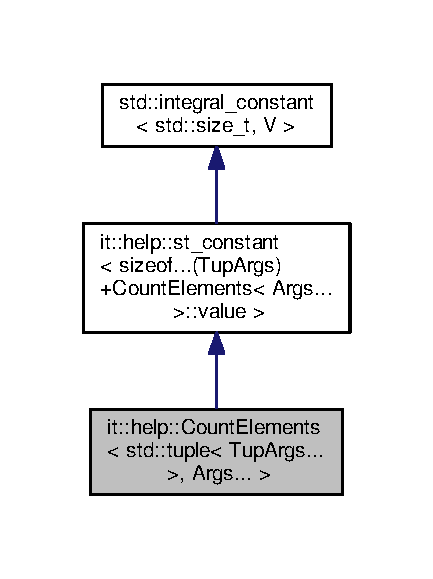
\includegraphics[width=208pt]{structit_1_1help_1_1CountElements_3_01std_1_1tuple_3_01TupArgs_8_8_8_01_4_00_01Args_8_8_8_01_4__inherit__graph}
\end{center}
\end{figure}


Collaboration diagram for it\+:\+:help\+:\+:Count\+Elements$<$ std\+:\+:tuple$<$ Tup\+Args... $>$, Args... $>$\+:\nopagebreak
\begin{figure}[H]
\begin{center}
\leavevmode
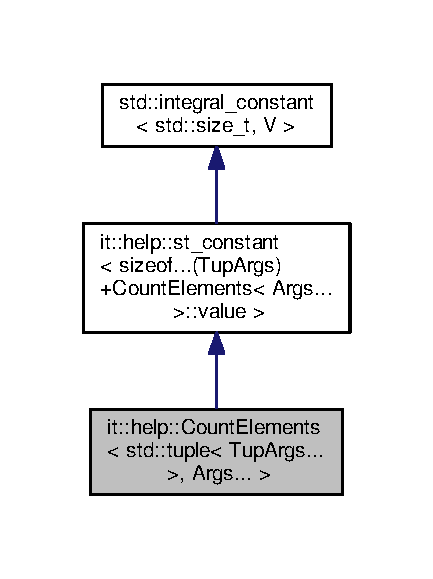
\includegraphics[width=208pt]{structit_1_1help_1_1CountElements_3_01std_1_1tuple_3_01TupArgs_8_8_8_01_4_00_01Args_8_8_8_01_4__coll__graph}
\end{center}
\end{figure}


The documentation for this struct was generated from the following file\+:\begin{DoxyCompactItemize}
\item 
/home/matheus/\+Algoritmos/\+C\+P\+P/\+Handy/include/\+Zip\+Iter/\hyperlink{ZipIter_2Helpers_8h}{Helpers.\+h}\end{DoxyCompactItemize}

\hypertarget{structit_1_1help_1_1CountElements_3_01T_00_01Args_8_8_8_01_4}{}\section{it\+:\+:help\+:\+:Count\+Elements$<$ T, Args... $>$ Struct Template Reference}
\label{structit_1_1help_1_1CountElements_3_01T_00_01Args_8_8_8_01_4}\index{it\+::help\+::\+Count\+Elements$<$ T, Args... $>$@{it\+::help\+::\+Count\+Elements$<$ T, Args... $>$}}


{\ttfamily \#include $<$Helpers.\+h$>$}



Inheritance diagram for it\+:\+:help\+:\+:Count\+Elements$<$ T, Args... $>$\+:\nopagebreak
\begin{figure}[H]
\begin{center}
\leavevmode
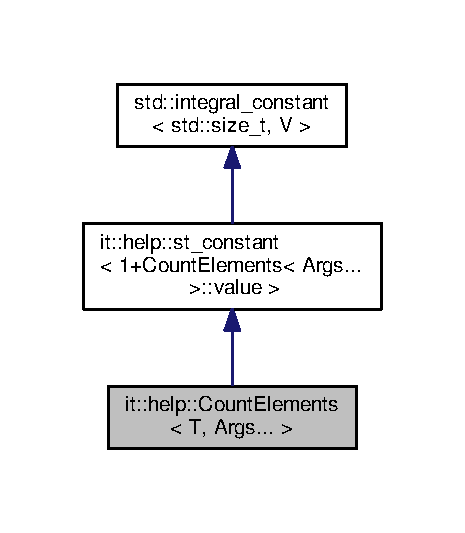
\includegraphics[width=223pt]{structit_1_1help_1_1CountElements_3_01T_00_01Args_8_8_8_01_4__inherit__graph}
\end{center}
\end{figure}


Collaboration diagram for it\+:\+:help\+:\+:Count\+Elements$<$ T, Args... $>$\+:\nopagebreak
\begin{figure}[H]
\begin{center}
\leavevmode
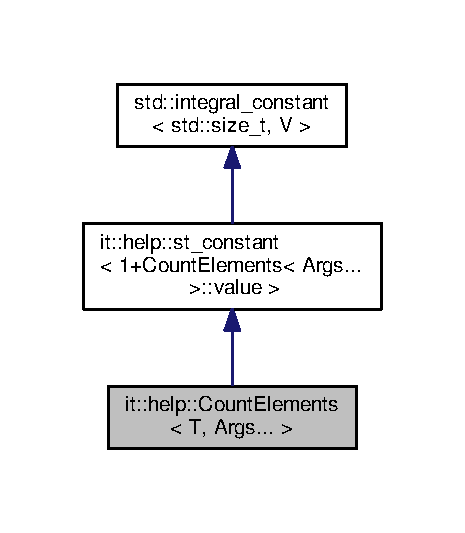
\includegraphics[width=223pt]{structit_1_1help_1_1CountElements_3_01T_00_01Args_8_8_8_01_4__coll__graph}
\end{center}
\end{figure}


The documentation for this struct was generated from the following file\+:\begin{DoxyCompactItemize}
\item 
/home/matheus/\+Algoritmos/\+C\+P\+P/\+Handy/include/\+Zip\+Iter/\hyperlink{ZipIter_2Helpers_8h}{Helpers.\+h}\end{DoxyCompactItemize}

\hypertarget{structit_1_1help_1_1CountElements_3_4}{}\section{it\+:\+:help\+:\+:Count\+Elements$<$$>$ Struct Template Reference}
\label{structit_1_1help_1_1CountElements_3_4}\index{it\+::help\+::\+Count\+Elements$<$$>$@{it\+::help\+::\+Count\+Elements$<$$>$}}


{\ttfamily \#include $<$Helpers.\+h$>$}



Inheritance diagram for it\+:\+:help\+:\+:Count\+Elements$<$$>$\+:\nopagebreak
\begin{figure}[H]
\begin{center}
\leavevmode
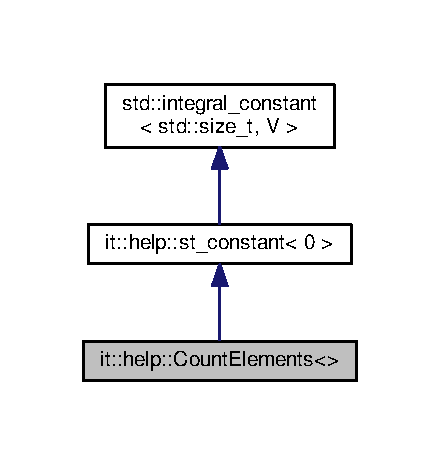
\includegraphics[width=211pt]{structit_1_1help_1_1CountElements_3_4__inherit__graph}
\end{center}
\end{figure}


Collaboration diagram for it\+:\+:help\+:\+:Count\+Elements$<$$>$\+:\nopagebreak
\begin{figure}[H]
\begin{center}
\leavevmode
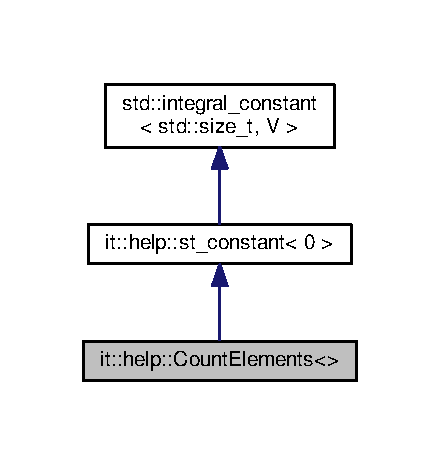
\includegraphics[width=211pt]{structit_1_1help_1_1CountElements_3_4__coll__graph}
\end{center}
\end{figure}


The documentation for this struct was generated from the following file\+:\begin{DoxyCompactItemize}
\item 
/home/matheus/\+Algoritmos/\+C\+P\+P/\+Handy/include/\+Zip\+Iter/\hyperlink{ZipIter_2Helpers_8h}{Helpers.\+h}\end{DoxyCompactItemize}

\hypertarget{structhandy_1_1Empty}{}\section{handy\+:\+:Empty$<$ typename $>$ Struct Template Reference}
\label{structhandy_1_1Empty}\index{handy\+::\+Empty$<$ typename $>$@{handy\+::\+Empty$<$ typename $>$}}


\hyperlink{structhandy_1_1Empty}{Empty} template base.  




{\ttfamily \#include $<$Helpers.\+h$>$}



\subsection{Detailed Description}
\subsubsection*{template$<$typename$>$\\*
struct handy\+::\+Empty$<$ typename $>$}

\hyperlink{structhandy_1_1Empty}{Empty} template base. 

The documentation for this struct was generated from the following file\+:\begin{DoxyCompactItemize}
\item 
/home/matheus/\+Algoritmos/\+C\+P\+P/\+Handy/include/\+Helpers/\hyperlink{Helpers_2Helpers_8h}{Helpers.\+h}\end{DoxyCompactItemize}

\hypertarget{structhandy_1_1GetArg}{}\section{handy\+:\+:Get\+Arg$<$ size\+\_\+t,... $>$ Struct Template Reference}
\label{structhandy_1_1GetArg}\index{handy\+::\+Get\+Arg$<$ size\+\_\+t,... $>$@{handy\+::\+Get\+Arg$<$ size\+\_\+t,... $>$}}


Base definition.  




{\ttfamily \#include $<$Helpers.\+h$>$}



\subsection{Detailed Description}
\subsubsection*{template$<$std\+::size\+\_\+t, typename...$>$\\*
struct handy\+::\+Get\+Arg$<$ size\+\_\+t,... $>$}

Base definition. 

The documentation for this struct was generated from the following file\+:\begin{DoxyCompactItemize}
\item 
/home/matheus/\+Algoritmos/\+C\+P\+P/\+Handy/include/\+Helpers/\hyperlink{Helpers_2Helpers_8h}{Helpers.\+h}\end{DoxyCompactItemize}

\hypertarget{structhandy_1_1GetArg_3_010_00_01T_00_01Args_8_8_8_01_4}{}\section{handy\+:\+:Get\+Arg$<$ 0, T, Args... $>$ Struct Template Reference}
\label{structhandy_1_1GetArg_3_010_00_01T_00_01Args_8_8_8_01_4}\index{handy\+::\+Get\+Arg$<$ 0, T, Args... $>$@{handy\+::\+Get\+Arg$<$ 0, T, Args... $>$}}


If {\ttfamily I} is 0, take type {\ttfamily T}.  




{\ttfamily \#include $<$Helpers.\+h$>$}

\subsection*{Public Types}
\begin{DoxyCompactItemize}
\item 
using \hyperlink{structhandy_1_1GetArg_3_010_00_01T_00_01Args_8_8_8_01_4_ac0c74cd6c4a9e2cc3c5c264f497ce11f}{type} = T
\end{DoxyCompactItemize}


\subsection{Detailed Description}
\subsubsection*{template$<$typename T, typename... Args$>$\\*
struct handy\+::\+Get\+Arg$<$ 0, T, Args... $>$}

If {\ttfamily I} is 0, take type {\ttfamily T}. 

\subsection{Member Typedef Documentation}
\index{handy\+::\+Get\+Arg$<$ 0, T, Args... $>$@{handy\+::\+Get\+Arg$<$ 0, T, Args... $>$}!type@{type}}
\index{type@{type}!handy\+::\+Get\+Arg$<$ 0, T, Args... $>$@{handy\+::\+Get\+Arg$<$ 0, T, Args... $>$}}
\subsubsection[{\texorpdfstring{type}{type}}]{\setlength{\rightskip}{0pt plus 5cm}template$<$typename T , typename... Args$>$ using {\bf handy\+::\+Get\+Arg}$<$ 0, T, Args... $>$\+::{\bf type} =  T}\hypertarget{structhandy_1_1GetArg_3_010_00_01T_00_01Args_8_8_8_01_4_ac0c74cd6c4a9e2cc3c5c264f497ce11f}{}\label{structhandy_1_1GetArg_3_010_00_01T_00_01Args_8_8_8_01_4_ac0c74cd6c4a9e2cc3c5c264f497ce11f}


The documentation for this struct was generated from the following file\+:\begin{DoxyCompactItemize}
\item 
/home/matheus/\+Algoritmos/\+C\+P\+P/\+Handy/include/\+Helpers/\hyperlink{Helpers_2Helpers_8h}{Helpers.\+h}\end{DoxyCompactItemize}

\hypertarget{structhandy_1_1GetArg_3_01I_01_4}{}\section{handy\+:\+:Get\+Arg$<$ I $>$ Struct Template Reference}
\label{structhandy_1_1GetArg_3_01I_01_4}\index{handy\+::\+Get\+Arg$<$ I $>$@{handy\+::\+Get\+Arg$<$ I $>$}}


If the initial {\ttfamily I} is greater than the number of arguments or is negative, throw an error.  




{\ttfamily \#include $<$Helpers.\+h$>$}



\subsection{Detailed Description}
\subsubsection*{template$<$std\+::size\+\_\+t I$>$\\*
struct handy\+::\+Get\+Arg$<$ I $>$}

If the initial {\ttfamily I} is greater than the number of arguments or is negative, throw an error. 

The documentation for this struct was generated from the following file\+:\begin{DoxyCompactItemize}
\item 
/home/matheus/\+Algoritmos/\+C\+P\+P/\+Handy/include/\+Helpers/\hyperlink{Helpers_2Helpers_8h}{Helpers.\+h}\end{DoxyCompactItemize}

\hypertarget{structhandy_1_1GetArg_3_01I_00_01T_00_01Args_8_8_8_01_4}{}\section{handy\+:\+:Get\+Arg$<$ I, T, Args... $>$ Struct Template Reference}
\label{structhandy_1_1GetArg_3_01I_00_01T_00_01Args_8_8_8_01_4}\index{handy\+::\+Get\+Arg$<$ I, T, Args... $>$@{handy\+::\+Get\+Arg$<$ I, T, Args... $>$}}


If {\ttfamily I} is not 0, take the type of \hyperlink{structhandy_1_1GetArg}{handy\+::\+Get\+Arg}$<$I-\/1, Args...$>$  




{\ttfamily \#include $<$Helpers.\+h$>$}

\subsection*{Public Types}
\begin{DoxyCompactItemize}
\item 
using \hyperlink{structhandy_1_1GetArg_3_01I_00_01T_00_01Args_8_8_8_01_4_a58d88c2429703df5203c70ab307813ab}{type} = typename \hyperlink{structhandy_1_1GetArg}{Get\+Arg}$<$ I-\/1, Args... $>$\+::\hyperlink{structhandy_1_1GetArg_3_01I_00_01T_00_01Args_8_8_8_01_4_a58d88c2429703df5203c70ab307813ab}{type}
\end{DoxyCompactItemize}


\subsection{Detailed Description}
\subsubsection*{template$<$std\+::size\+\_\+t I, typename T, typename... Args$>$\\*
struct handy\+::\+Get\+Arg$<$ I, T, Args... $>$}

If {\ttfamily I} is not 0, take the type of \hyperlink{structhandy_1_1GetArg}{handy\+::\+Get\+Arg}$<$I-\/1, Args...$>$ 

\subsection{Member Typedef Documentation}
\index{handy\+::\+Get\+Arg$<$ I, T, Args... $>$@{handy\+::\+Get\+Arg$<$ I, T, Args... $>$}!type@{type}}
\index{type@{type}!handy\+::\+Get\+Arg$<$ I, T, Args... $>$@{handy\+::\+Get\+Arg$<$ I, T, Args... $>$}}
\subsubsection[{\texorpdfstring{type}{type}}]{\setlength{\rightskip}{0pt plus 5cm}template$<$std\+::size\+\_\+t I, typename T , typename... Args$>$ using {\bf handy\+::\+Get\+Arg}$<$ I, T, Args... $>$\+::{\bf type} =  typename {\bf Get\+Arg}$<$I-\/1, Args...$>$\+::{\bf type}}\hypertarget{structhandy_1_1GetArg_3_01I_00_01T_00_01Args_8_8_8_01_4_a58d88c2429703df5203c70ab307813ab}{}\label{structhandy_1_1GetArg_3_01I_00_01T_00_01Args_8_8_8_01_4_a58d88c2429703df5203c70ab307813ab}


The documentation for this struct was generated from the following file\+:\begin{DoxyCompactItemize}
\item 
/home/matheus/\+Algoritmos/\+C\+P\+P/\+Handy/include/\+Helpers/\hyperlink{Helpers_2Helpers_8h}{Helpers.\+h}\end{DoxyCompactItemize}

\hypertarget{structhandy_1_1impl_1_1HalfClosedInterval}{}\section{handy\+:\+:impl\+:\+:Half\+Closed\+Interval Struct Reference}
\label{structhandy_1_1impl_1_1HalfClosedInterval}\index{handy\+::impl\+::\+Half\+Closed\+Interval@{handy\+::impl\+::\+Half\+Closed\+Interval}}


{\ttfamily \#include $<$Range.\+h$>$}

\subsection*{Public Member Functions}
\begin{DoxyCompactItemize}
\item 
{\footnotesize template$<$typename T $>$ }\\bool \hyperlink{structhandy_1_1impl_1_1HalfClosedInterval_a6d3e8dcfab037b3c16b2babc689ea372}{operator()} (const T \&first, const T \&last, const T \&step) const 
\end{DoxyCompactItemize}


\subsection{Member Function Documentation}
\index{handy\+::impl\+::\+Half\+Closed\+Interval@{handy\+::impl\+::\+Half\+Closed\+Interval}!operator()@{operator()}}
\index{operator()@{operator()}!handy\+::impl\+::\+Half\+Closed\+Interval@{handy\+::impl\+::\+Half\+Closed\+Interval}}
\subsubsection[{\texorpdfstring{operator()(const T \&first, const T \&last, const T \&step) const }{operator()(const T &first, const T &last, const T &step) const }}]{\setlength{\rightskip}{0pt plus 5cm}template$<$typename T $>$ bool handy\+::impl\+::\+Half\+Closed\+Interval\+::operator() (
\begin{DoxyParamCaption}
\item[{const T \&}]{first, }
\item[{const T \&}]{last, }
\item[{const T \&}]{step}
\end{DoxyParamCaption}
) const\hspace{0.3cm}{\ttfamily [inline]}}\hypertarget{structhandy_1_1impl_1_1HalfClosedInterval_a6d3e8dcfab037b3c16b2babc689ea372}{}\label{structhandy_1_1impl_1_1HalfClosedInterval_a6d3e8dcfab037b3c16b2babc689ea372}


The documentation for this struct was generated from the following file\+:\begin{DoxyCompactItemize}
\item 
/home/matheus/\+Algoritmos/\+C\+P\+P/\+Handy/include/\+Range/\hyperlink{Range_8h}{Range.\+h}\end{DoxyCompactItemize}

\hypertarget{structhandy_1_1impl_1_1InfiniteInterval}{}\section{handy\+:\+:impl\+:\+:Infinite\+Interval Struct Reference}
\label{structhandy_1_1impl_1_1InfiniteInterval}\index{handy\+::impl\+::\+Infinite\+Interval@{handy\+::impl\+::\+Infinite\+Interval}}


{\ttfamily \#include $<$Range.\+h$>$}

\subsection*{Public Member Functions}
\begin{DoxyCompactItemize}
\item 
{\footnotesize template$<$typename T $>$ }\\constexpr bool \hyperlink{structhandy_1_1impl_1_1InfiniteInterval_a258e99ad1f61bfdf4189307c24d3ff90}{operator()} (const T \&, const T \&, const T \&) const 
\end{DoxyCompactItemize}


\subsection{Member Function Documentation}
\index{handy\+::impl\+::\+Infinite\+Interval@{handy\+::impl\+::\+Infinite\+Interval}!operator()@{operator()}}
\index{operator()@{operator()}!handy\+::impl\+::\+Infinite\+Interval@{handy\+::impl\+::\+Infinite\+Interval}}
\subsubsection[{\texorpdfstring{operator()(const T \&, const T \&, const T \&) const }{operator()(const T &, const T &, const T &) const }}]{\setlength{\rightskip}{0pt plus 5cm}template$<$typename T $>$ constexpr bool handy\+::impl\+::\+Infinite\+Interval\+::operator() (
\begin{DoxyParamCaption}
\item[{const T \&}]{, }
\item[{const T \&}]{, }
\item[{const T \&}]{}
\end{DoxyParamCaption}
) const\hspace{0.3cm}{\ttfamily [inline]}}\hypertarget{structhandy_1_1impl_1_1InfiniteInterval_a258e99ad1f61bfdf4189307c24d3ff90}{}\label{structhandy_1_1impl_1_1InfiniteInterval_a258e99ad1f61bfdf4189307c24d3ff90}


The documentation for this struct was generated from the following file\+:\begin{DoxyCompactItemize}
\item 
/home/matheus/\+Algoritmos/\+C\+P\+P/\+Handy/include/\+Range/\hyperlink{Range_8h}{Range.\+h}\end{DoxyCompactItemize}

\hypertarget{structcnt_1_1help_1_1IntegralType}{}\section{cnt\+:\+:help\+:\+:Integral\+Type Struct Reference}
\label{structcnt_1_1help_1_1IntegralType}\index{cnt\+::help\+::\+Integral\+Type@{cnt\+::help\+::\+Integral\+Type}}


{\ttfamily \#include $<$Helpers.\+h$>$}



\subsection{Detailed Description}
These are dummy classes that help to create functions to treat the type of parameters of the accessors\+: integrals, iterables or iterators. 

The documentation for this struct was generated from the following file\+:\begin{DoxyCompactItemize}
\item 
/home/matheus/\+Algoritmos/\+C\+P\+P/\+Handy/include/\+Container/\hyperlink{Container_2Helpers_8h}{Helpers.\+h}\end{DoxyCompactItemize}

\hypertarget{structhandy_1_1IsContainer}{}\section{handy\+:\+:Is\+Container$<$ T $>$ Struct Template Reference}
\label{structhandy_1_1IsContainer}\index{handy\+::\+Is\+Container$<$ T $>$@{handy\+::\+Is\+Container$<$ T $>$}}


{\ttfamily \#include $<$Algorithms.\+h$>$}



Inheritance diagram for handy\+:\+:Is\+Container$<$ T $>$\+:\nopagebreak
\begin{figure}[H]
\begin{center}
\leavevmode
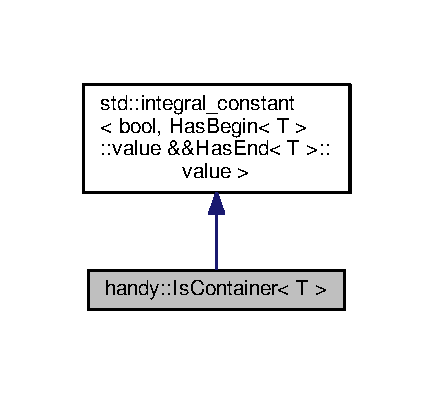
\includegraphics[width=208pt]{structhandy_1_1IsContainer__inherit__graph}
\end{center}
\end{figure}


Collaboration diagram for handy\+:\+:Is\+Container$<$ T $>$\+:\nopagebreak
\begin{figure}[H]
\begin{center}
\leavevmode
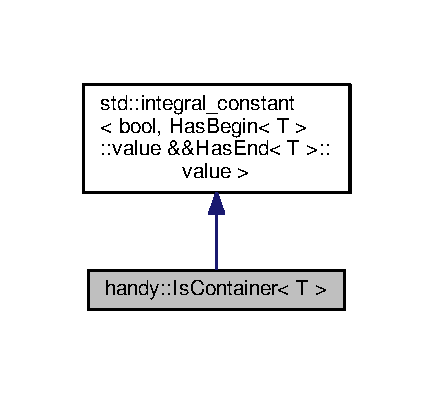
\includegraphics[width=208pt]{structhandy_1_1IsContainer__coll__graph}
\end{center}
\end{figure}


The documentation for this struct was generated from the following file\+:\begin{DoxyCompactItemize}
\item 
/home/matheus/\+Algoritmos/\+C\+P\+P/\+Handy/include/\+Algorithms/\hyperlink{Algorithms_8h}{Algorithms.\+h}\end{DoxyCompactItemize}

\hypertarget{structhandy_1_1impl_1_1IsInherited}{}\section{handy\+:\+:impl\+:\+:Is\+Inherited$<$ T, U, Template $>$ Struct Template Reference}
\label{structhandy_1_1impl_1_1IsInherited}\index{handy\+::impl\+::\+Is\+Inherited$<$ T, U, Template $>$@{handy\+::impl\+::\+Is\+Inherited$<$ T, U, Template $>$}}


Tells if {\ttfamily T} inherits from {\ttfamily U}, or from a template {\ttfamily Template$<$\+W$>$}. In the case where {\ttfamily T} is the same as {\ttfamily U}, \hyperlink{structhandy_1_1impl_1_1IsInherited_ade331c690ccfcc4c9fbe160b83f9491ba3347f5ab27dd0282a949005f868dcde7}{value } is {\ttfamily true}.  




{\ttfamily \#include $<$Helpers.\+h$>$}



Inheritance diagram for handy\+:\+:impl\+:\+:Is\+Inherited$<$ T, U, Template $>$\+:\nopagebreak
\begin{figure}[H]
\begin{center}
\leavevmode
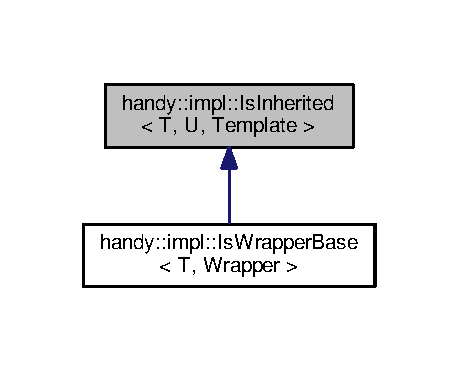
\includegraphics[width=220pt]{structhandy_1_1impl_1_1IsInherited__inherit__graph}
\end{center}
\end{figure}
\subsection*{Public Types}
\begin{DoxyCompactItemize}
\item 
enum \{ \hyperlink{structhandy_1_1impl_1_1IsInherited_ade331c690ccfcc4c9fbe160b83f9491ba3347f5ab27dd0282a949005f868dcde7}{value} = decltype(is\+Inherited(std\+:\+:declval$<$std\+:\+:decay\+\_\+t$<$T$>$$>$()))\+:\+:value
 \}
\end{DoxyCompactItemize}
\subsection*{Static Public Member Functions}
\begin{DoxyCompactItemize}
\item 
{\footnotesize template$<$typename W $>$ }\\static constexpr {\bf std\+::true\+\_\+type} \hyperlink{structhandy_1_1impl_1_1IsInherited_ab35b0bbac7a0a30321f1e9f97f66c9c4}{is\+Inherited} (Template$<$ W $>$)
\begin{DoxyCompactList}\small\item\em Returns {\ttfamily true} if {\ttfamily T} inherits from the template {\ttfamily Template$<$\+W$>$} \end{DoxyCompactList}\item 
static constexpr {\bf std\+::true\+\_\+type} \hyperlink{structhandy_1_1impl_1_1IsInherited_ad6960a3bde384c00493a40cf4f6cbd23}{is\+Inherited} (const std\+::decay\+\_\+t$<$ U $>$ \&)
\begin{DoxyCompactList}\small\item\em Returns {\ttfamily true} if {\ttfamily T} inherits from {\ttfamily U}. \end{DoxyCompactList}\item 
static constexpr {\bf std\+::false\+\_\+type} \hyperlink{structhandy_1_1impl_1_1IsInherited_acc033894644bd14ea55b4963e1f4f040}{is\+Inherited} (...)
\begin{DoxyCompactList}\small\item\em Returns {\ttfamily false} otherwise. \end{DoxyCompactList}\end{DoxyCompactItemize}


\subsection{Detailed Description}
\subsubsection*{template$<$class T, class U = std\+::nullptr\+\_\+t, template$<$ typename $>$ class Template = Empty$>$\\*
struct handy\+::impl\+::\+Is\+Inherited$<$ T, U, Template $>$}

Tells if {\ttfamily T} inherits from {\ttfamily U}, or from a template {\ttfamily Template$<$\+W$>$}. In the case where {\ttfamily T} is the same as {\ttfamily U}, \hyperlink{structhandy_1_1impl_1_1IsInherited_ade331c690ccfcc4c9fbe160b83f9491ba3347f5ab27dd0282a949005f868dcde7}{value } is {\ttfamily true}. 


\begin{DoxyTemplParams}{Template Parameters}
{\em T} & Derived class to check \\
\hline
{\em U} & Possible base class \\
\hline
{\em Template} & Possible Template base class \\
\hline
\end{DoxyTemplParams}


\subsection{Member Enumeration Documentation}
\subsubsection[{\texorpdfstring{anonymous enum}{anonymous enum}}]{\setlength{\rightskip}{0pt plus 5cm}template$<$class T , class U  = std\+::nullptr\+\_\+t, template$<$ typename $>$ class Template = Empty$>$ anonymous enum}\hypertarget{structhandy_1_1impl_1_1IsInherited_ade331c690ccfcc4c9fbe160b83f9491b}{}\label{structhandy_1_1impl_1_1IsInherited_ade331c690ccfcc4c9fbe160b83f9491b}
\begin{Desc}
\item[Enumerator]\par
\begin{description}
\index{value@{value}!handy\+::impl\+::\+Is\+Inherited@{handy\+::impl\+::\+Is\+Inherited}}\index{handy\+::impl\+::\+Is\+Inherited@{handy\+::impl\+::\+Is\+Inherited}!value@{value}}\item[{\em 
value\hypertarget{structhandy_1_1impl_1_1IsInherited_ade331c690ccfcc4c9fbe160b83f9491ba3347f5ab27dd0282a949005f868dcde7}{}\label{structhandy_1_1impl_1_1IsInherited_ade331c690ccfcc4c9fbe160b83f9491ba3347f5ab27dd0282a949005f868dcde7}
}]Saves the value returned by \hyperlink{structhandy_1_1impl_1_1IsInherited_ab35b0bbac7a0a30321f1e9f97f66c9c4}{is\+Inherited()} \end{description}
\end{Desc}


\subsection{Member Function Documentation}
\index{handy\+::impl\+::\+Is\+Inherited@{handy\+::impl\+::\+Is\+Inherited}!is\+Inherited@{is\+Inherited}}
\index{is\+Inherited@{is\+Inherited}!handy\+::impl\+::\+Is\+Inherited@{handy\+::impl\+::\+Is\+Inherited}}
\subsubsection[{\texorpdfstring{is\+Inherited(\+Template$<$ W $>$)}{isInherited(Template< W >)}}]{\setlength{\rightskip}{0pt plus 5cm}template$<$class T , class U  = std\+::nullptr\+\_\+t, template$<$ typename $>$ class Template = Empty$>$ template$<$typename W $>$ static constexpr {\bf std\+::true\+\_\+type} {\bf handy\+::impl\+::\+Is\+Inherited}$<$ T, U, Template $>$\+::is\+Inherited (
\begin{DoxyParamCaption}
\item[{Template$<$ W $>$}]{}
\end{DoxyParamCaption}
)\hspace{0.3cm}{\ttfamily [static]}}\hypertarget{structhandy_1_1impl_1_1IsInherited_ab35b0bbac7a0a30321f1e9f97f66c9c4}{}\label{structhandy_1_1impl_1_1IsInherited_ab35b0bbac7a0a30321f1e9f97f66c9c4}


Returns {\ttfamily true} if {\ttfamily T} inherits from the template {\ttfamily Template$<$\+W$>$} 

\index{handy\+::impl\+::\+Is\+Inherited@{handy\+::impl\+::\+Is\+Inherited}!is\+Inherited@{is\+Inherited}}
\index{is\+Inherited@{is\+Inherited}!handy\+::impl\+::\+Is\+Inherited@{handy\+::impl\+::\+Is\+Inherited}}
\subsubsection[{\texorpdfstring{is\+Inherited(const std\+::decay\+\_\+t$<$ U $>$ \&)}{isInherited(const std::decay_t< U > &)}}]{\setlength{\rightskip}{0pt plus 5cm}template$<$class T , class U  = std\+::nullptr\+\_\+t, template$<$ typename $>$ class Template = Empty$>$ static constexpr {\bf std\+::true\+\_\+type} {\bf handy\+::impl\+::\+Is\+Inherited}$<$ T, U, Template $>$\+::is\+Inherited (
\begin{DoxyParamCaption}
\item[{const std\+::decay\+\_\+t$<$ U $>$ \&}]{}
\end{DoxyParamCaption}
)\hspace{0.3cm}{\ttfamily [static]}}\hypertarget{structhandy_1_1impl_1_1IsInherited_ad6960a3bde384c00493a40cf4f6cbd23}{}\label{structhandy_1_1impl_1_1IsInherited_ad6960a3bde384c00493a40cf4f6cbd23}


Returns {\ttfamily true} if {\ttfamily T} inherits from {\ttfamily U}. 

\index{handy\+::impl\+::\+Is\+Inherited@{handy\+::impl\+::\+Is\+Inherited}!is\+Inherited@{is\+Inherited}}
\index{is\+Inherited@{is\+Inherited}!handy\+::impl\+::\+Is\+Inherited@{handy\+::impl\+::\+Is\+Inherited}}
\subsubsection[{\texorpdfstring{is\+Inherited(...)}{isInherited(...)}}]{\setlength{\rightskip}{0pt plus 5cm}template$<$class T , class U  = std\+::nullptr\+\_\+t, template$<$ typename $>$ class Template = Empty$>$ static constexpr {\bf std\+::false\+\_\+type} {\bf handy\+::impl\+::\+Is\+Inherited}$<$ T, U, Template $>$\+::is\+Inherited (
\begin{DoxyParamCaption}
\item[{}]{...}
\end{DoxyParamCaption}
)\hspace{0.3cm}{\ttfamily [static]}}\hypertarget{structhandy_1_1impl_1_1IsInherited_acc033894644bd14ea55b4963e1f4f040}{}\label{structhandy_1_1impl_1_1IsInherited_acc033894644bd14ea55b4963e1f4f040}


Returns {\ttfamily false} otherwise. 



The documentation for this struct was generated from the following file\+:\begin{DoxyCompactItemize}
\item 
/home/matheus/\+Algoritmos/\+C\+P\+P/\+Handy/include/\+Helpers/\hyperlink{Helpers_2Helpers_8h}{Helpers.\+h}\end{DoxyCompactItemize}

\hypertarget{structhandy_1_1IsSpecialization}{}\section{handy\+:\+:Is\+Specialization$<$ T, Template $>$ Struct Template Reference}
\label{structhandy_1_1IsSpecialization}\index{handy\+::\+Is\+Specialization$<$ T, Template $>$@{handy\+::\+Is\+Specialization$<$ T, Template $>$}}


Check for template specialization.  




{\ttfamily \#include $<$Helpers.\+h$>$}



Inheritance diagram for handy\+:\+:Is\+Specialization$<$ T, Template $>$\+:\nopagebreak
\begin{figure}[H]
\begin{center}
\leavevmode
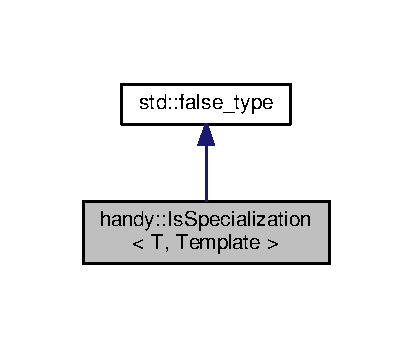
\includegraphics[width=198pt]{structhandy_1_1IsSpecialization__inherit__graph}
\end{center}
\end{figure}


Collaboration diagram for handy\+:\+:Is\+Specialization$<$ T, Template $>$\+:\nopagebreak
\begin{figure}[H]
\begin{center}
\leavevmode
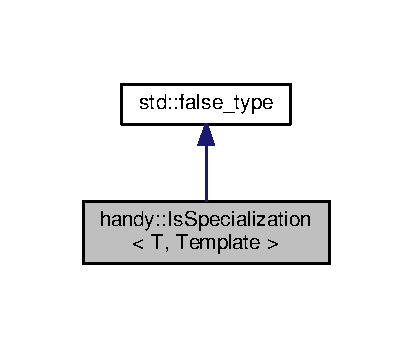
\includegraphics[width=198pt]{structhandy_1_1IsSpecialization__coll__graph}
\end{center}
\end{figure}


\subsection{Detailed Description}
\subsubsection*{template$<$typename T, template$<$ typename... $>$ class Template$>$\\*
struct handy\+::\+Is\+Specialization$<$ T, Template $>$}

Check for template specialization. 


\begin{DoxyTemplParams}{Template Parameters}
{\em T} & Type to check \\
\hline
{\em Template} & Template type to check \\
\hline
\end{DoxyTemplParams}
\begin{DoxyNote}{Note}
Taken from \href{https://bitbucket.org/martinhofernandes/wheels/src/default/include/wheels/meta/type_traits.h%2B%2B?fileviewer=file-view-default#cl-161}{\tt https\+://bitbucket.\+org/martinhofernandes/wheels/src/default/include/wheels/meta/type\+\_\+traits.\+h\%2\+B\%2\+B?fileviewer=file-\/view-\/default\#cl-\/161}
\end{DoxyNote}
If class {\ttfamily T} is not a specialization of template {\ttfamily Template}, inherit from {\bf std\+::false\+\_\+type} 

The documentation for this struct was generated from the following file\+:\begin{DoxyCompactItemize}
\item 
/home/matheus/\+Algoritmos/\+C\+P\+P/\+Handy/include/\+Helpers/\hyperlink{Helpers_2Helpers_8h}{Helpers.\+h}\end{DoxyCompactItemize}

\hypertarget{structhandy_1_1IsSpecialization_3_01Template_3_01Args_8_8_8_01_4_00_01Template_01_4}{}\section{handy\+:\+:Is\+Specialization$<$ Template$<$ Args... $>$, Template $>$ Struct Template Reference}
\label{structhandy_1_1IsSpecialization_3_01Template_3_01Args_8_8_8_01_4_00_01Template_01_4}\index{handy\+::\+Is\+Specialization$<$ Template$<$ Args... $>$, Template $>$@{handy\+::\+Is\+Specialization$<$ Template$<$ Args... $>$, Template $>$}}


Check for template specialization.  




{\ttfamily \#include $<$Helpers.\+h$>$}



Inheritance diagram for handy\+:\+:Is\+Specialization$<$ Template$<$ Args... $>$, Template $>$\+:\nopagebreak
\begin{figure}[H]
\begin{center}
\leavevmode
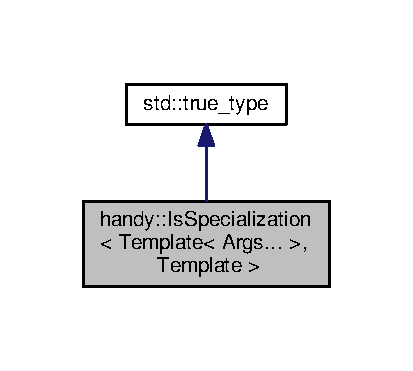
\includegraphics[width=198pt]{structhandy_1_1IsSpecialization_3_01Template_3_01Args_8_8_8_01_4_00_01Template_01_4__inherit__graph}
\end{center}
\end{figure}


Collaboration diagram for handy\+:\+:Is\+Specialization$<$ Template$<$ Args... $>$, Template $>$\+:\nopagebreak
\begin{figure}[H]
\begin{center}
\leavevmode
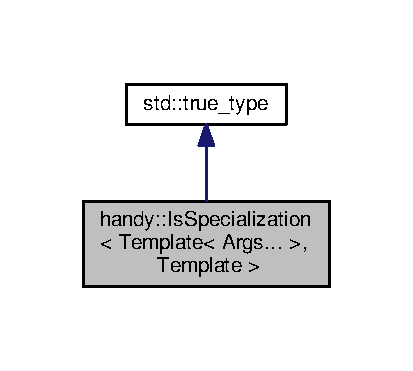
\includegraphics[width=198pt]{structhandy_1_1IsSpecialization_3_01Template_3_01Args_8_8_8_01_4_00_01Template_01_4__coll__graph}
\end{center}
\end{figure}


\subsection{Detailed Description}
\subsubsection*{template$<$template$<$ typename... $>$ class Template, typename... Args$>$\\*
struct handy\+::\+Is\+Specialization$<$ Template$<$ Args... $>$, Template $>$}

Check for template specialization. 


\begin{DoxyTemplParams}{Template Parameters}
{\em T} & Type to check \\
\hline
{\em Template} & Template type to check \\
\hline
\end{DoxyTemplParams}
\begin{DoxyNote}{Note}
Taken from \href{https://bitbucket.org/martinhofernandes/wheels/src/default/include/wheels/meta/type_traits.h%2B%2B?fileviewer=file-view-default#cl-161}{\tt https\+://bitbucket.\+org/martinhofernandes/wheels/src/default/include/wheels/meta/type\+\_\+traits.\+h\%2\+B\%2\+B?fileviewer=file-\/view-\/default\#cl-\/161}
\end{DoxyNote}
If class {\ttfamily T} is a specialization of template {\ttfamily Template}, inherit from {\bf std\+::true\+\_\+type} 

The documentation for this struct was generated from the following file\+:\begin{DoxyCompactItemize}
\item 
/home/matheus/\+Algoritmos/\+C\+P\+P/\+Handy/include/\+Helpers/\hyperlink{Helpers_2Helpers_8h}{Helpers.\+h}\end{DoxyCompactItemize}

\hypertarget{classIsSpecializationDoc}{}\section{Is\+Specialization\+Doc Class Reference}
\label{classIsSpecializationDoc}\index{Is\+Specialization\+Doc@{Is\+Specialization\+Doc}}


Check for template specialization.  




{\ttfamily \#include $<$Helpers.\+h$>$}



\subsection{Detailed Description}
Check for template specialization. 


\begin{DoxyTemplParams}{Template Parameters}
{\em T} & Type to check \\
\hline
{\em Template} & Template type to check \\
\hline
\end{DoxyTemplParams}
\begin{DoxyNote}{Note}
Taken from \href{https://bitbucket.org/martinhofernandes/wheels/src/default/include/wheels/meta/type_traits.h%2B%2B?fileviewer=file-view-default#cl-161}{\tt https\+://bitbucket.\+org/martinhofernandes/wheels/src/default/include/wheels/meta/type\+\_\+traits.\+h\%2\+B\%2\+B?fileviewer=file-\/view-\/default\#cl-\/161} 
\end{DoxyNote}


The documentation for this class was generated from the following file\+:\begin{DoxyCompactItemize}
\item 
/home/matheus/\+Algoritmos/\+C\+P\+P/\+Handy/include/\+Helpers/\hyperlink{Helpers_2Helpers_8h}{Helpers.\+h}\end{DoxyCompactItemize}

\hypertarget{structhandy_1_1impl_1_1IsWrapper}{}\section{handy\+:\+:impl\+:\+:Is\+Wrapper$<$ T $>$ Struct Template Reference}
\label{structhandy_1_1impl_1_1IsWrapper}\index{handy\+::impl\+::\+Is\+Wrapper$<$ T $>$@{handy\+::impl\+::\+Is\+Wrapper$<$ T $>$}}


{\ttfamily \#include $<$Helpers.\+h$>$}



Inheritance diagram for handy\+:\+:impl\+:\+:Is\+Wrapper$<$ T $>$\+:\nopagebreak
\begin{figure}[H]
\begin{center}
\leavevmode
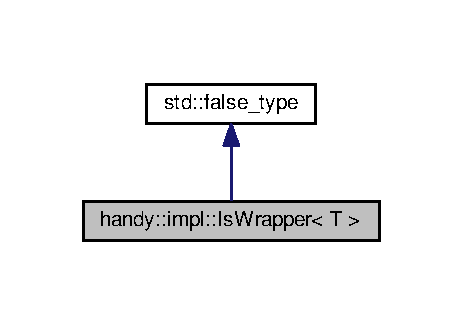
\includegraphics[width=222pt]{structhandy_1_1impl_1_1IsWrapper__inherit__graph}
\end{center}
\end{figure}


Collaboration diagram for handy\+:\+:impl\+:\+:Is\+Wrapper$<$ T $>$\+:\nopagebreak
\begin{figure}[H]
\begin{center}
\leavevmode
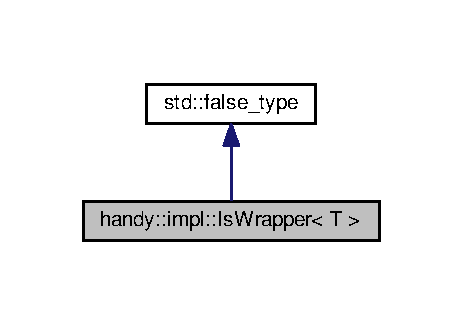
\includegraphics[width=222pt]{structhandy_1_1impl_1_1IsWrapper__coll__graph}
\end{center}
\end{figure}


The documentation for this struct was generated from the following file\+:\begin{DoxyCompactItemize}
\item 
/home/matheus/\+Algoritmos/\+C\+P\+P/\+Handy/include/\+Wrapper/\hyperlink{Wrapper_2Helpers_8h}{Helpers.\+h}\end{DoxyCompactItemize}

\hypertarget{structhandy_1_1impl_1_1IsWrapper_3_01Wrapper_3_01T_01_4_01_4}{}\section{handy\+:\+:impl\+:\+:Is\+Wrapper$<$ Wrapper$<$ T $>$ $>$ Struct Template Reference}
\label{structhandy_1_1impl_1_1IsWrapper_3_01Wrapper_3_01T_01_4_01_4}\index{handy\+::impl\+::\+Is\+Wrapper$<$ Wrapper$<$ T $>$ $>$@{handy\+::impl\+::\+Is\+Wrapper$<$ Wrapper$<$ T $>$ $>$}}


{\ttfamily \#include $<$Helpers.\+h$>$}



Inheritance diagram for handy\+:\+:impl\+:\+:Is\+Wrapper$<$ Wrapper$<$ T $>$ $>$\+:\nopagebreak
\begin{figure}[H]
\begin{center}
\leavevmode
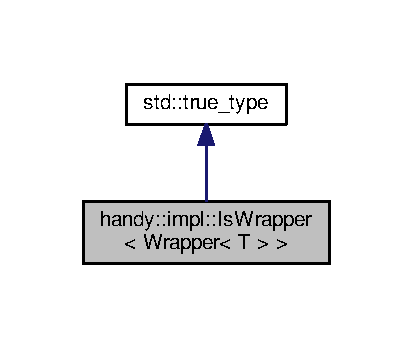
\includegraphics[width=198pt]{structhandy_1_1impl_1_1IsWrapper_3_01Wrapper_3_01T_01_4_01_4__inherit__graph}
\end{center}
\end{figure}


Collaboration diagram for handy\+:\+:impl\+:\+:Is\+Wrapper$<$ Wrapper$<$ T $>$ $>$\+:\nopagebreak
\begin{figure}[H]
\begin{center}
\leavevmode
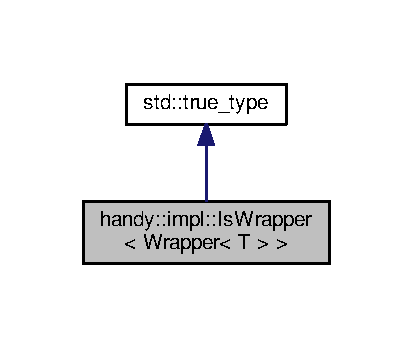
\includegraphics[width=198pt]{structhandy_1_1impl_1_1IsWrapper_3_01Wrapper_3_01T_01_4_01_4__coll__graph}
\end{center}
\end{figure}


The documentation for this struct was generated from the following file\+:\begin{DoxyCompactItemize}
\item 
/home/matheus/\+Algoritmos/\+C\+P\+P/\+Handy/include/\+Wrapper/\hyperlink{Wrapper_2Helpers_8h}{Helpers.\+h}\end{DoxyCompactItemize}

\hypertarget{structhandy_1_1impl_1_1IsWrapperBase}{}\section{handy\+:\+:impl\+:\+:Is\+Wrapper\+Base$<$ T $>$ Struct Template Reference}
\label{structhandy_1_1impl_1_1IsWrapperBase}\index{handy\+::impl\+::\+Is\+Wrapper\+Base$<$ T $>$@{handy\+::impl\+::\+Is\+Wrapper\+Base$<$ T $>$}}


{\ttfamily \#include $<$Helpers.\+h$>$}



Inheritance diagram for handy\+:\+:impl\+:\+:Is\+Wrapper\+Base$<$ T $>$\+:\nopagebreak
\begin{figure}[H]
\begin{center}
\leavevmode
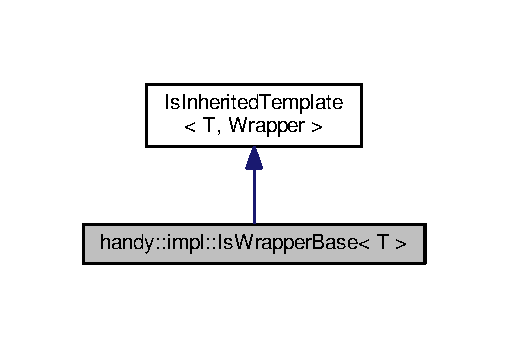
\includegraphics[width=244pt]{structhandy_1_1impl_1_1IsWrapperBase__inherit__graph}
\end{center}
\end{figure}


Collaboration diagram for handy\+:\+:impl\+:\+:Is\+Wrapper\+Base$<$ T $>$\+:\nopagebreak
\begin{figure}[H]
\begin{center}
\leavevmode
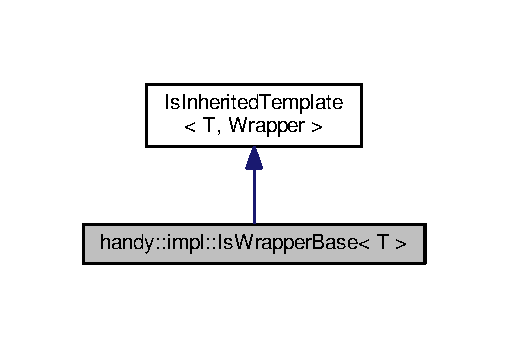
\includegraphics[width=244pt]{structhandy_1_1impl_1_1IsWrapperBase__coll__graph}
\end{center}
\end{figure}
\subsection*{Additional Inherited Members}


The documentation for this struct was generated from the following file\+:\begin{DoxyCompactItemize}
\item 
/home/matheus/\+Algoritmos/\+C\+P\+P/\+Handy/include/\+Wrapper/\hyperlink{Wrapper_2Helpers_8h}{Helpers.\+h}\end{DoxyCompactItemize}

\hypertarget{structit_1_1help_1_1Iterable}{}\section{it\+:\+:help\+:\+:Iterable$<$ T $>$ Struct Template Reference}
\label{structit_1_1help_1_1Iterable}\index{it\+::help\+::\+Iterable$<$ T $>$@{it\+::help\+::\+Iterable$<$ T $>$}}


Simple trait for defining iterable types.  




{\ttfamily \#include $<$Helpers.\+h$>$}

\subsection*{Public Types}
\begin{DoxyCompactItemize}
\item 
using \hyperlink{structit_1_1help_1_1Iterable_ae119f8a540d8b116afb5a0153c6f6c8a}{iterator} = typename T\+::iterator
\end{DoxyCompactItemize}


\subsection{Detailed Description}
\subsubsection*{template$<$typename T$>$\\*
struct it\+::help\+::\+Iterable$<$ T $>$}

Simple trait for defining iterable types. 

\subsection{Member Typedef Documentation}
\index{it\+::help\+::\+Iterable@{it\+::help\+::\+Iterable}!iterator@{iterator}}
\index{iterator@{iterator}!it\+::help\+::\+Iterable@{it\+::help\+::\+Iterable}}
\subsubsection[{\texorpdfstring{iterator}{iterator}}]{\setlength{\rightskip}{0pt plus 5cm}template$<$typename T $>$ using {\bf it\+::help\+::\+Iterable}$<$ T $>$\+::{\bf iterator} =  typename T\+::iterator}\hypertarget{structit_1_1help_1_1Iterable_ae119f8a540d8b116afb5a0153c6f6c8a}{}\label{structit_1_1help_1_1Iterable_ae119f8a540d8b116afb5a0153c6f6c8a}


The documentation for this struct was generated from the following file\+:\begin{DoxyCompactItemize}
\item 
/home/matheus/\+Algoritmos/\+C\+P\+P/\+Handy/include/\+Zip\+Iter/\hyperlink{ZipIter_2Helpers_8h}{Helpers.\+h}\end{DoxyCompactItemize}

\hypertarget{structit_1_1help_1_1Iterable_3_01const_01T_01_5_01_4}{}\section{it\+:\+:help\+:\+:Iterable$<$ const T $\ast$ $>$ Struct Template Reference}
\label{structit_1_1help_1_1Iterable_3_01const_01T_01_5_01_4}\index{it\+::help\+::\+Iterable$<$ const T $\ast$ $>$@{it\+::help\+::\+Iterable$<$ const T $\ast$ $>$}}


{\ttfamily \#include $<$Helpers.\+h$>$}

\subsection*{Public Types}
\begin{DoxyCompactItemize}
\item 
using \hyperlink{structit_1_1help_1_1Iterable_3_01const_01T_01_5_01_4_ae1c626ae93b53f527f15dfe9341ce555}{iterator} = const T $\ast$
\end{DoxyCompactItemize}


\subsection{Member Typedef Documentation}
\index{it\+::help\+::\+Iterable$<$ const T $\ast$ $>$@{it\+::help\+::\+Iterable$<$ const T $\ast$ $>$}!iterator@{iterator}}
\index{iterator@{iterator}!it\+::help\+::\+Iterable$<$ const T $\ast$ $>$@{it\+::help\+::\+Iterable$<$ const T $\ast$ $>$}}
\subsubsection[{\texorpdfstring{iterator}{iterator}}]{\setlength{\rightskip}{0pt plus 5cm}template$<$typename T $>$ using {\bf it\+::help\+::\+Iterable}$<$ const T $\ast$ $>$\+::{\bf iterator} =  const T$\ast$}\hypertarget{structit_1_1help_1_1Iterable_3_01const_01T_01_5_01_4_ae1c626ae93b53f527f15dfe9341ce555}{}\label{structit_1_1help_1_1Iterable_3_01const_01T_01_5_01_4_ae1c626ae93b53f527f15dfe9341ce555}


The documentation for this struct was generated from the following file\+:\begin{DoxyCompactItemize}
\item 
/home/matheus/\+Algoritmos/\+C\+P\+P/\+Handy/include/\+Zip\+Iter/\hyperlink{ZipIter_2Helpers_8h}{Helpers.\+h}\end{DoxyCompactItemize}

\hypertarget{structit_1_1help_1_1Iterable_3_01const_01T_01_4}{}\section{it\+:\+:help\+:\+:Iterable$<$ const T $>$ Struct Template Reference}
\label{structit_1_1help_1_1Iterable_3_01const_01T_01_4}\index{it\+::help\+::\+Iterable$<$ const T $>$@{it\+::help\+::\+Iterable$<$ const T $>$}}


{\ttfamily \#include $<$Helpers.\+h$>$}

\subsection*{Public Types}
\begin{DoxyCompactItemize}
\item 
using \hyperlink{structit_1_1help_1_1Iterable_3_01const_01T_01_4_aed9d4b32ea0d0cff09b6193be5f5ae58}{iterator} = typename T\+::const\+\_\+iterator
\end{DoxyCompactItemize}


\subsection{Member Typedef Documentation}
\index{it\+::help\+::\+Iterable$<$ const T $>$@{it\+::help\+::\+Iterable$<$ const T $>$}!iterator@{iterator}}
\index{iterator@{iterator}!it\+::help\+::\+Iterable$<$ const T $>$@{it\+::help\+::\+Iterable$<$ const T $>$}}
\subsubsection[{\texorpdfstring{iterator}{iterator}}]{\setlength{\rightskip}{0pt plus 5cm}template$<$typename T $>$ using {\bf it\+::help\+::\+Iterable}$<$ const T $>$\+::{\bf iterator} =  typename T\+::const\+\_\+iterator}\hypertarget{structit_1_1help_1_1Iterable_3_01const_01T_01_4_aed9d4b32ea0d0cff09b6193be5f5ae58}{}\label{structit_1_1help_1_1Iterable_3_01const_01T_01_4_aed9d4b32ea0d0cff09b6193be5f5ae58}


The documentation for this struct was generated from the following file\+:\begin{DoxyCompactItemize}
\item 
/home/matheus/\+Algoritmos/\+C\+P\+P/\+Handy/include/\+Zip\+Iter/\hyperlink{ZipIter_2Helpers_8h}{Helpers.\+h}\end{DoxyCompactItemize}

\hypertarget{structit_1_1help_1_1Iterable_3_01const_01T[N]_4}{}\section{it\+:\+:help\+:\+:Iterable$<$ const T\mbox{[}N\mbox{]}$>$ Struct Template Reference}
\label{structit_1_1help_1_1Iterable_3_01const_01T[N]_4}\index{it\+::help\+::\+Iterable$<$ const T\mbox{[}\+N\mbox{]}$>$@{it\+::help\+::\+Iterable$<$ const T[N]$>$}}


{\ttfamily \#include $<$Helpers.\+h$>$}

\subsection*{Public Types}
\begin{DoxyCompactItemize}
\item 
using \hyperlink{structit_1_1help_1_1Iterable_3_01const_01T[N]_4_ab130f7ca6f5e168697eee8ba64273278}{iterator} = const T $\ast$
\end{DoxyCompactItemize}


\subsection{Member Typedef Documentation}
\index{it\+::help\+::\+Iterable$<$ const T\mbox{[}\+N\mbox{]}$>$@{it\+::help\+::\+Iterable$<$ const T[N]$>$}!iterator@{iterator}}
\index{iterator@{iterator}!it\+::help\+::\+Iterable$<$ const T\mbox{[}\+N\mbox{]}$>$@{it\+::help\+::\+Iterable$<$ const T[N]$>$}}
\subsubsection[{\texorpdfstring{iterator}{iterator}}]{\setlength{\rightskip}{0pt plus 5cm}template$<$typename T , std\+::size\+\_\+t N$>$ using {\bf it\+::help\+::\+Iterable}$<$ const T\mbox{[}N\mbox{]}$>$\+::{\bf iterator} =  const T$\ast$}\hypertarget{structit_1_1help_1_1Iterable_3_01const_01T[N]_4_ab130f7ca6f5e168697eee8ba64273278}{}\label{structit_1_1help_1_1Iterable_3_01const_01T[N]_4_ab130f7ca6f5e168697eee8ba64273278}


The documentation for this struct was generated from the following file\+:\begin{DoxyCompactItemize}
\item 
/home/matheus/\+Algoritmos/\+C\+P\+P/\+Handy/include/\+Zip\+Iter/\hyperlink{ZipIter_2Helpers_8h}{Helpers.\+h}\end{DoxyCompactItemize}

\hypertarget{structit_1_1help_1_1Iterable_3_01T_01_5_01_4}{}\section{it\+:\+:help\+:\+:Iterable$<$ T $\ast$ $>$ Struct Template Reference}
\label{structit_1_1help_1_1Iterable_3_01T_01_5_01_4}\index{it\+::help\+::\+Iterable$<$ T $\ast$ $>$@{it\+::help\+::\+Iterable$<$ T $\ast$ $>$}}


{\ttfamily \#include $<$Helpers.\+h$>$}

\subsection*{Public Types}
\begin{DoxyCompactItemize}
\item 
using \hyperlink{structit_1_1help_1_1Iterable_3_01T_01_5_01_4_a8358e383286cbe494802cbbac75fd894}{iterator} = T $\ast$
\end{DoxyCompactItemize}


\subsection{Member Typedef Documentation}
\index{it\+::help\+::\+Iterable$<$ T $\ast$ $>$@{it\+::help\+::\+Iterable$<$ T $\ast$ $>$}!iterator@{iterator}}
\index{iterator@{iterator}!it\+::help\+::\+Iterable$<$ T $\ast$ $>$@{it\+::help\+::\+Iterable$<$ T $\ast$ $>$}}
\subsubsection[{\texorpdfstring{iterator}{iterator}}]{\setlength{\rightskip}{0pt plus 5cm}template$<$typename T $>$ using {\bf it\+::help\+::\+Iterable}$<$ T $\ast$ $>$\+::{\bf iterator} =  T$\ast$}\hypertarget{structit_1_1help_1_1Iterable_3_01T_01_5_01_4_a8358e383286cbe494802cbbac75fd894}{}\label{structit_1_1help_1_1Iterable_3_01T_01_5_01_4_a8358e383286cbe494802cbbac75fd894}


The documentation for this struct was generated from the following file\+:\begin{DoxyCompactItemize}
\item 
/home/matheus/\+Algoritmos/\+C\+P\+P/\+Handy/include/\+Zip\+Iter/\hyperlink{ZipIter_2Helpers_8h}{Helpers.\+h}\end{DoxyCompactItemize}

\hypertarget{structit_1_1help_1_1Iterable_3_01T[N]_4}{}\section{it\+:\+:help\+:\+:Iterable$<$ T\mbox{[}N\mbox{]}$>$ Struct Template Reference}
\label{structit_1_1help_1_1Iterable_3_01T[N]_4}\index{it\+::help\+::\+Iterable$<$ T\mbox{[}\+N\mbox{]}$>$@{it\+::help\+::\+Iterable$<$ T[N]$>$}}


{\ttfamily \#include $<$Helpers.\+h$>$}

\subsection*{Public Types}
\begin{DoxyCompactItemize}
\item 
using \hyperlink{structit_1_1help_1_1Iterable_3_01T[N]_4_a36024509bbcde977155c3c244a5fa219}{iterator} = T $\ast$
\end{DoxyCompactItemize}


\subsection{Member Typedef Documentation}
\index{it\+::help\+::\+Iterable$<$ T\mbox{[}\+N\mbox{]}$>$@{it\+::help\+::\+Iterable$<$ T[N]$>$}!iterator@{iterator}}
\index{iterator@{iterator}!it\+::help\+::\+Iterable$<$ T\mbox{[}\+N\mbox{]}$>$@{it\+::help\+::\+Iterable$<$ T[N]$>$}}
\subsubsection[{\texorpdfstring{iterator}{iterator}}]{\setlength{\rightskip}{0pt plus 5cm}template$<$typename T , std\+::size\+\_\+t N$>$ using {\bf it\+::help\+::\+Iterable}$<$ T\mbox{[}N\mbox{]}$>$\+::{\bf iterator} =  T$\ast$}\hypertarget{structit_1_1help_1_1Iterable_3_01T[N]_4_a36024509bbcde977155c3c244a5fa219}{}\label{structit_1_1help_1_1Iterable_3_01T[N]_4_a36024509bbcde977155c3c244a5fa219}


The documentation for this struct was generated from the following file\+:\begin{DoxyCompactItemize}
\item 
/home/matheus/\+Algoritmos/\+C\+P\+P/\+Handy/include/\+Zip\+Iter/\hyperlink{ZipIter_2Helpers_8h}{Helpers.\+h}\end{DoxyCompactItemize}

\hypertarget{structcnt_1_1help_1_1IterableType}{}\section{cnt\+:\+:help\+:\+:Iterable\+Type Struct Reference}
\label{structcnt_1_1help_1_1IterableType}\index{cnt\+::help\+::\+Iterable\+Type@{cnt\+::help\+::\+Iterable\+Type}}


{\ttfamily \#include $<$Helpers.\+h$>$}



The documentation for this struct was generated from the following file\+:\begin{DoxyCompactItemize}
\item 
/home/matheus/\+Algoritmos/\+C\+P\+P/\+Handy/include/\+Container/\hyperlink{Container_2Helpers_8h}{Helpers.\+h}\end{DoxyCompactItemize}

\hypertarget{classhandy_1_1Range_1_1Iterator}{}\section{handy\+:\+:Range$<$ T, Valid\+Range $>$\+:\+:Iterator Class Reference}
\label{classhandy_1_1Range_1_1Iterator}\index{handy\+::\+Range$<$ T, Valid\+Range $>$\+::\+Iterator@{handy\+::\+Range$<$ T, Valid\+Range $>$\+::\+Iterator}}


{\ttfamily \#include $<$Range.\+h$>$}



Inheritance diagram for handy\+:\+:Range$<$ T, Valid\+Range $>$\+:\+:Iterator\+:\nopagebreak
\begin{figure}[H]
\begin{center}
\leavevmode
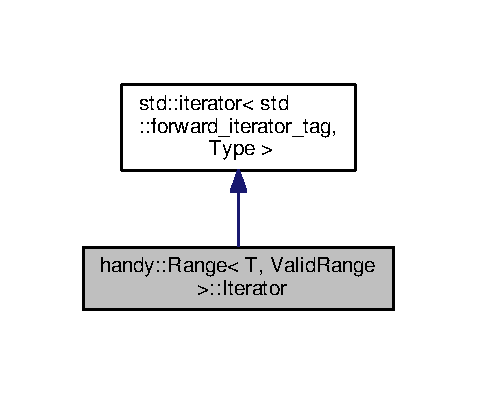
\includegraphics[width=229pt]{classhandy_1_1Range_1_1Iterator__inherit__graph}
\end{center}
\end{figure}


Collaboration diagram for handy\+:\+:Range$<$ T, Valid\+Range $>$\+:\+:Iterator\+:\nopagebreak
\begin{figure}[H]
\begin{center}
\leavevmode
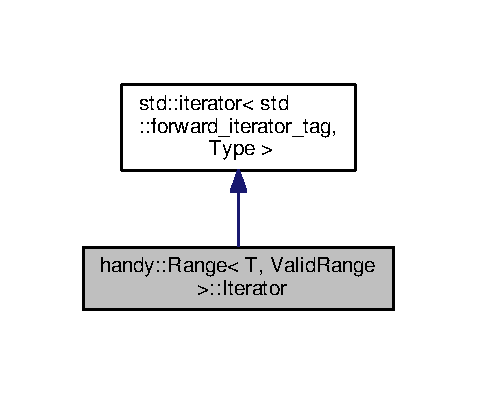
\includegraphics[width=229pt]{classhandy_1_1Range_1_1Iterator__coll__graph}
\end{center}
\end{figure}
\subsection*{Public Types}
\begin{DoxyCompactItemize}
\item 
using \hyperlink{classhandy_1_1Range_1_1Iterator_ae982d471802ac0e3746e326c3aa2fc14}{Base} = {\bf std\+::iterator}$<$ {\bf std\+::forward\+\_\+iterator\+\_\+tag}, \hyperlink{classhandy_1_1Range_a2a8c2d169657c93464989e7608ed3f9b}{Type} $>$
\item 
using \hyperlink{classhandy_1_1Range_1_1Iterator_a99f227df409cebfc6fa8250b5868e8a3}{value\+\_\+type} = typename Base\+::reference
\item 
using \hyperlink{classhandy_1_1Range_1_1Iterator_ab182b2493e468efbced9983e3e38dbe4}{reference} = typename Base\+::reference
\item 
using \hyperlink{classhandy_1_1Range_1_1Iterator_a2a4a02c25dce296702ceb66fe75f9918}{pointer} = typename Base\+::pointer
\item 
using \hyperlink{classhandy_1_1Range_1_1Iterator_ac7bf1cb755fa3ca0f213b19f0fdbe8de}{difference\+\_\+type} = typename Base\+::difference\+\_\+type
\item 
using \hyperlink{classhandy_1_1Range_1_1Iterator_a5e9da733ea7dadc2cc69327288e3e7a2}{iterator\+\_\+category} = typename Base\+::iterator\+\_\+category
\end{DoxyCompactItemize}
\subsection*{Public Member Functions}
\begin{DoxyCompactItemize}
\item 
\hyperlink{classhandy_1_1Range_1_1Iterator_a5eb5d28d949109bb56b42eff6be76372}{Iterator} (const \hyperlink{classhandy_1_1Range}{Range} \&range, \hyperlink{classhandy_1_1Range_a2a8c2d169657c93464989e7608ed3f9b}{Type} value)
\item 
\hyperlink{classhandy_1_1Range_1_1Iterator_ab182b2493e468efbced9983e3e38dbe4}{reference} \hyperlink{classhandy_1_1Range_1_1Iterator_a9e860c6771882cb760d1bc394294cc15}{operator$\ast$} ()
\begin{DoxyCompactList}\small\item\em Forward iterator. \end{DoxyCompactList}\item 
\hyperlink{classhandy_1_1Range_1_1Iterator_a2a4a02c25dce296702ceb66fe75f9918}{pointer} \hyperlink{classhandy_1_1Range_1_1Iterator_a2edb437146413ea9114ec92b02cee8bc}{operator-\/$>$} ()
\item 
\hyperlink{classhandy_1_1Range_1_1Iterator}{Iterator} \hyperlink{classhandy_1_1Range_1_1Iterator_ab813ce87299a9ac40a26f0027854c6e4}{operator++} ()
\item 
\hyperlink{classhandy_1_1Range_1_1Iterator}{Iterator} \hyperlink{classhandy_1_1Range_1_1Iterator_aeea6305a195e7f3d9b09204fbf7c1448}{operator++} (int)
\item 
bool \hyperlink{classhandy_1_1Range_1_1Iterator_a38fa4d55b0f9dda5cd2af504a909cef1}{operator==} (const \hyperlink{classhandy_1_1Range_1_1Iterator}{Iterator} \&it) const 
\item 
bool \hyperlink{classhandy_1_1Range_1_1Iterator_afa581bd5ba90ea8930361e287283a820}{operator!=} (const \hyperlink{classhandy_1_1Range_1_1Iterator}{Iterator} \&it) const 
\end{DoxyCompactItemize}


\subsection{Member Typedef Documentation}
\index{handy\+::\+Range\+::\+Iterator@{handy\+::\+Range\+::\+Iterator}!Base@{Base}}
\index{Base@{Base}!handy\+::\+Range\+::\+Iterator@{handy\+::\+Range\+::\+Iterator}}
\subsubsection[{\texorpdfstring{Base}{Base}}]{\setlength{\rightskip}{0pt plus 5cm}template$<$typename T, typename Valid\+Range = impl\+::\+Half\+Closed\+Interval$>$ using {\bf handy\+::\+Range}$<$ T, Valid\+Range $>$\+::{\bf Iterator\+::\+Base} =  {\bf std\+::iterator}$<${\bf std\+::forward\+\_\+iterator\+\_\+tag}, {\bf Type}$>$}\hypertarget{classhandy_1_1Range_1_1Iterator_ae982d471802ac0e3746e326c3aa2fc14}{}\label{classhandy_1_1Range_1_1Iterator_ae982d471802ac0e3746e326c3aa2fc14}
\index{handy\+::\+Range\+::\+Iterator@{handy\+::\+Range\+::\+Iterator}!difference\+\_\+type@{difference\+\_\+type}}
\index{difference\+\_\+type@{difference\+\_\+type}!handy\+::\+Range\+::\+Iterator@{handy\+::\+Range\+::\+Iterator}}
\subsubsection[{\texorpdfstring{difference\+\_\+type}{difference_type}}]{\setlength{\rightskip}{0pt plus 5cm}template$<$typename T, typename Valid\+Range = impl\+::\+Half\+Closed\+Interval$>$ using {\bf handy\+::\+Range}$<$ T, Valid\+Range $>$\+::{\bf Iterator\+::difference\+\_\+type} =  typename Base\+::difference\+\_\+type}\hypertarget{classhandy_1_1Range_1_1Iterator_ac7bf1cb755fa3ca0f213b19f0fdbe8de}{}\label{classhandy_1_1Range_1_1Iterator_ac7bf1cb755fa3ca0f213b19f0fdbe8de}
\index{handy\+::\+Range\+::\+Iterator@{handy\+::\+Range\+::\+Iterator}!iterator\+\_\+category@{iterator\+\_\+category}}
\index{iterator\+\_\+category@{iterator\+\_\+category}!handy\+::\+Range\+::\+Iterator@{handy\+::\+Range\+::\+Iterator}}
\subsubsection[{\texorpdfstring{iterator\+\_\+category}{iterator_category}}]{\setlength{\rightskip}{0pt plus 5cm}template$<$typename T, typename Valid\+Range = impl\+::\+Half\+Closed\+Interval$>$ using {\bf handy\+::\+Range}$<$ T, Valid\+Range $>$\+::{\bf Iterator\+::iterator\+\_\+category} =  typename Base\+::iterator\+\_\+category}\hypertarget{classhandy_1_1Range_1_1Iterator_a5e9da733ea7dadc2cc69327288e3e7a2}{}\label{classhandy_1_1Range_1_1Iterator_a5e9da733ea7dadc2cc69327288e3e7a2}
\index{handy\+::\+Range\+::\+Iterator@{handy\+::\+Range\+::\+Iterator}!pointer@{pointer}}
\index{pointer@{pointer}!handy\+::\+Range\+::\+Iterator@{handy\+::\+Range\+::\+Iterator}}
\subsubsection[{\texorpdfstring{pointer}{pointer}}]{\setlength{\rightskip}{0pt plus 5cm}template$<$typename T, typename Valid\+Range = impl\+::\+Half\+Closed\+Interval$>$ using {\bf handy\+::\+Range}$<$ T, Valid\+Range $>$\+::{\bf Iterator\+::pointer} =  typename Base\+::pointer}\hypertarget{classhandy_1_1Range_1_1Iterator_a2a4a02c25dce296702ceb66fe75f9918}{}\label{classhandy_1_1Range_1_1Iterator_a2a4a02c25dce296702ceb66fe75f9918}
\index{handy\+::\+Range\+::\+Iterator@{handy\+::\+Range\+::\+Iterator}!reference@{reference}}
\index{reference@{reference}!handy\+::\+Range\+::\+Iterator@{handy\+::\+Range\+::\+Iterator}}
\subsubsection[{\texorpdfstring{reference}{reference}}]{\setlength{\rightskip}{0pt plus 5cm}template$<$typename T, typename Valid\+Range = impl\+::\+Half\+Closed\+Interval$>$ using {\bf handy\+::\+Range}$<$ T, Valid\+Range $>$\+::{\bf Iterator\+::reference} =  typename Base\+::reference}\hypertarget{classhandy_1_1Range_1_1Iterator_ab182b2493e468efbced9983e3e38dbe4}{}\label{classhandy_1_1Range_1_1Iterator_ab182b2493e468efbced9983e3e38dbe4}
\index{handy\+::\+Range\+::\+Iterator@{handy\+::\+Range\+::\+Iterator}!value\+\_\+type@{value\+\_\+type}}
\index{value\+\_\+type@{value\+\_\+type}!handy\+::\+Range\+::\+Iterator@{handy\+::\+Range\+::\+Iterator}}
\subsubsection[{\texorpdfstring{value\+\_\+type}{value_type}}]{\setlength{\rightskip}{0pt plus 5cm}template$<$typename T, typename Valid\+Range = impl\+::\+Half\+Closed\+Interval$>$ using {\bf handy\+::\+Range}$<$ T, Valid\+Range $>$\+::{\bf Iterator\+::value\+\_\+type} =  typename Base\+::reference}\hypertarget{classhandy_1_1Range_1_1Iterator_a99f227df409cebfc6fa8250b5868e8a3}{}\label{classhandy_1_1Range_1_1Iterator_a99f227df409cebfc6fa8250b5868e8a3}


\subsection{Constructor \& Destructor Documentation}
\index{handy\+::\+Range\+::\+Iterator@{handy\+::\+Range\+::\+Iterator}!Iterator@{Iterator}}
\index{Iterator@{Iterator}!handy\+::\+Range\+::\+Iterator@{handy\+::\+Range\+::\+Iterator}}
\subsubsection[{\texorpdfstring{Iterator(const Range \&range, Type value)}{Iterator(const Range &range, Type value)}}]{\setlength{\rightskip}{0pt plus 5cm}template$<$typename T, typename Valid\+Range = impl\+::\+Half\+Closed\+Interval$>$ {\bf handy\+::\+Range}$<$ T, Valid\+Range $>$\+::Iterator\+::\+Iterator (
\begin{DoxyParamCaption}
\item[{const {\bf Range} \&}]{range, }
\item[{{\bf Type}}]{value}
\end{DoxyParamCaption}
)\hspace{0.3cm}{\ttfamily [inline]}}\hypertarget{classhandy_1_1Range_1_1Iterator_a5eb5d28d949109bb56b42eff6be76372}{}\label{classhandy_1_1Range_1_1Iterator_a5eb5d28d949109bb56b42eff6be76372}


\subsection{Member Function Documentation}
\index{handy\+::\+Range\+::\+Iterator@{handy\+::\+Range\+::\+Iterator}!operator"!=@{operator"!=}}
\index{operator"!=@{operator"!=}!handy\+::\+Range\+::\+Iterator@{handy\+::\+Range\+::\+Iterator}}
\subsubsection[{\texorpdfstring{operator"!=(const Iterator \&it) const }{operator!=(const Iterator &it) const }}]{\setlength{\rightskip}{0pt plus 5cm}template$<$typename T, typename Valid\+Range = impl\+::\+Half\+Closed\+Interval$>$ bool {\bf handy\+::\+Range}$<$ T, Valid\+Range $>$\+::Iterator\+::operator!= (
\begin{DoxyParamCaption}
\item[{const {\bf Iterator} \&}]{it}
\end{DoxyParamCaption}
) const\hspace{0.3cm}{\ttfamily [inline]}}\hypertarget{classhandy_1_1Range_1_1Iterator_afa581bd5ba90ea8930361e287283a820}{}\label{classhandy_1_1Range_1_1Iterator_afa581bd5ba90ea8930361e287283a820}
\index{handy\+::\+Range\+::\+Iterator@{handy\+::\+Range\+::\+Iterator}!operator$\ast$@{operator$\ast$}}
\index{operator$\ast$@{operator$\ast$}!handy\+::\+Range\+::\+Iterator@{handy\+::\+Range\+::\+Iterator}}
\subsubsection[{\texorpdfstring{operator$\ast$()}{operator*()}}]{\setlength{\rightskip}{0pt plus 5cm}template$<$typename T, typename Valid\+Range = impl\+::\+Half\+Closed\+Interval$>$ {\bf reference} {\bf handy\+::\+Range}$<$ T, Valid\+Range $>$\+::Iterator\+::operator$\ast$ (
\begin{DoxyParamCaption}
{}
\end{DoxyParamCaption}
)\hspace{0.3cm}{\ttfamily [inline]}}\hypertarget{classhandy_1_1Range_1_1Iterator_a9e860c6771882cb760d1bc394294cc15}{}\label{classhandy_1_1Range_1_1Iterator_a9e860c6771882cb760d1bc394294cc15}


Forward iterator. 

\index{handy\+::\+Range\+::\+Iterator@{handy\+::\+Range\+::\+Iterator}!operator++@{operator++}}
\index{operator++@{operator++}!handy\+::\+Range\+::\+Iterator@{handy\+::\+Range\+::\+Iterator}}
\subsubsection[{\texorpdfstring{operator++()}{operator++()}}]{\setlength{\rightskip}{0pt plus 5cm}template$<$typename T, typename Valid\+Range = impl\+::\+Half\+Closed\+Interval$>$ {\bf Iterator} {\bf handy\+::\+Range}$<$ T, Valid\+Range $>$\+::Iterator\+::operator++ (
\begin{DoxyParamCaption}
{}
\end{DoxyParamCaption}
)\hspace{0.3cm}{\ttfamily [inline]}}\hypertarget{classhandy_1_1Range_1_1Iterator_ab813ce87299a9ac40a26f0027854c6e4}{}\label{classhandy_1_1Range_1_1Iterator_ab813ce87299a9ac40a26f0027854c6e4}
\index{handy\+::\+Range\+::\+Iterator@{handy\+::\+Range\+::\+Iterator}!operator++@{operator++}}
\index{operator++@{operator++}!handy\+::\+Range\+::\+Iterator@{handy\+::\+Range\+::\+Iterator}}
\subsubsection[{\texorpdfstring{operator++(int)}{operator++(int)}}]{\setlength{\rightskip}{0pt plus 5cm}template$<$typename T, typename Valid\+Range = impl\+::\+Half\+Closed\+Interval$>$ {\bf Iterator} {\bf handy\+::\+Range}$<$ T, Valid\+Range $>$\+::Iterator\+::operator++ (
\begin{DoxyParamCaption}
\item[{int}]{}
\end{DoxyParamCaption}
)\hspace{0.3cm}{\ttfamily [inline]}}\hypertarget{classhandy_1_1Range_1_1Iterator_aeea6305a195e7f3d9b09204fbf7c1448}{}\label{classhandy_1_1Range_1_1Iterator_aeea6305a195e7f3d9b09204fbf7c1448}
\index{handy\+::\+Range\+::\+Iterator@{handy\+::\+Range\+::\+Iterator}!operator-\/$>$@{operator-\/$>$}}
\index{operator-\/$>$@{operator-\/$>$}!handy\+::\+Range\+::\+Iterator@{handy\+::\+Range\+::\+Iterator}}
\subsubsection[{\texorpdfstring{operator-\/$>$()}{operator->()}}]{\setlength{\rightskip}{0pt plus 5cm}template$<$typename T, typename Valid\+Range = impl\+::\+Half\+Closed\+Interval$>$ {\bf pointer} {\bf handy\+::\+Range}$<$ T, Valid\+Range $>$\+::Iterator\+::operator-\/$>$ (
\begin{DoxyParamCaption}
{}
\end{DoxyParamCaption}
)\hspace{0.3cm}{\ttfamily [inline]}}\hypertarget{classhandy_1_1Range_1_1Iterator_a2edb437146413ea9114ec92b02cee8bc}{}\label{classhandy_1_1Range_1_1Iterator_a2edb437146413ea9114ec92b02cee8bc}
\index{handy\+::\+Range\+::\+Iterator@{handy\+::\+Range\+::\+Iterator}!operator==@{operator==}}
\index{operator==@{operator==}!handy\+::\+Range\+::\+Iterator@{handy\+::\+Range\+::\+Iterator}}
\subsubsection[{\texorpdfstring{operator==(const Iterator \&it) const }{operator==(const Iterator &it) const }}]{\setlength{\rightskip}{0pt plus 5cm}template$<$typename T, typename Valid\+Range = impl\+::\+Half\+Closed\+Interval$>$ bool {\bf handy\+::\+Range}$<$ T, Valid\+Range $>$\+::Iterator\+::operator== (
\begin{DoxyParamCaption}
\item[{const {\bf Iterator} \&}]{it}
\end{DoxyParamCaption}
) const\hspace{0.3cm}{\ttfamily [inline]}}\hypertarget{classhandy_1_1Range_1_1Iterator_a38fa4d55b0f9dda5cd2af504a909cef1}{}\label{classhandy_1_1Range_1_1Iterator_a38fa4d55b0f9dda5cd2af504a909cef1}


The documentation for this class was generated from the following file\+:\begin{DoxyCompactItemize}
\item 
/home/matheus/\+Algoritmos/\+C\+P\+P/\+Handy/include/\+Range/\hyperlink{Range_8h}{Range.\+h}\end{DoxyCompactItemize}

\hypertarget{structcnt_1_1help_1_1IteratorType}{}\section{cnt\+:\+:help\+:\+:Iterator\+Type Struct Reference}
\label{structcnt_1_1help_1_1IteratorType}\index{cnt\+::help\+::\+Iterator\+Type@{cnt\+::help\+::\+Iterator\+Type}}


{\ttfamily \#include $<$Helpers.\+h$>$}



The documentation for this struct was generated from the following file\+:\begin{DoxyCompactItemize}
\item 
/home/matheus/\+Algoritmos/\+C\+P\+P/\+Handy/include/\+Container/\hyperlink{Container_2Helpers_8h}{Helpers.\+h}\end{DoxyCompactItemize}

\hypertarget{structcnt_1_1help_1_1multiply}{}\section{cnt\+:\+:help\+:\+:multiply$<$... $>$ Struct Template Reference}
\label{structcnt_1_1help_1_1multiply}\index{cnt\+::help\+::multiply$<$... $>$@{cnt\+::help\+::multiply$<$... $>$}}


{\ttfamily \#include $<$Helpers.\+h$>$}



\subsection{Detailed Description}
\subsubsection*{template$<$std\+::size\+\_\+t...$>$\\*
struct cnt\+::help\+::multiply$<$... $>$}

Multiply the integers to get the total size at compile time. If no argument is give, the function returns 0


\begin{DoxyParams}[1]{Parameters}
\mbox{\tt in}  & {\em Is} & The variadic arguments \\
\hline
\end{DoxyParams}
\begin{DoxyReturn}{Returns}
The total size of multiplying Is or 0, if sizeof...(Is) == 0 
\end{DoxyReturn}


The documentation for this struct was generated from the following file\+:\begin{DoxyCompactItemize}
\item 
/home/matheus/\+Algoritmos/\+C\+P\+P/\+Handy/include/\+Container/\hyperlink{Container_2Helpers_8h}{Helpers.\+h}\end{DoxyCompactItemize}

\hypertarget{structcnt_1_1help_1_1multiply_3_01I_00_01Is_8_8_8_01_4}{}\section{cnt\+:\+:help\+:\+:multiply$<$ I, Is... $>$ Struct Template Reference}
\label{structcnt_1_1help_1_1multiply_3_01I_00_01Is_8_8_8_01_4}\index{cnt\+::help\+::multiply$<$ I, Is... $>$@{cnt\+::help\+::multiply$<$ I, Is... $>$}}


{\ttfamily \#include $<$Helpers.\+h$>$}



Inheritance diagram for cnt\+:\+:help\+:\+:multiply$<$ I, Is... $>$\+:\nopagebreak
\begin{figure}[H]
\begin{center}
\leavevmode
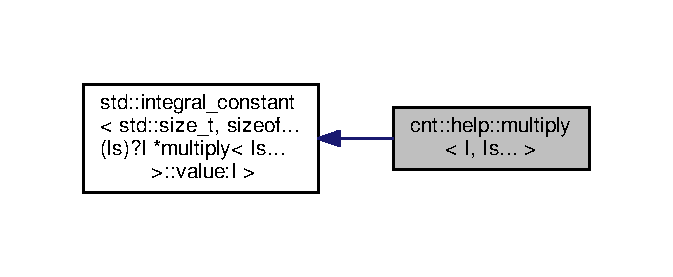
\includegraphics[width=323pt]{structcnt_1_1help_1_1multiply_3_01I_00_01Is_8_8_8_01_4__inherit__graph}
\end{center}
\end{figure}


Collaboration diagram for cnt\+:\+:help\+:\+:multiply$<$ I, Is... $>$\+:\nopagebreak
\begin{figure}[H]
\begin{center}
\leavevmode
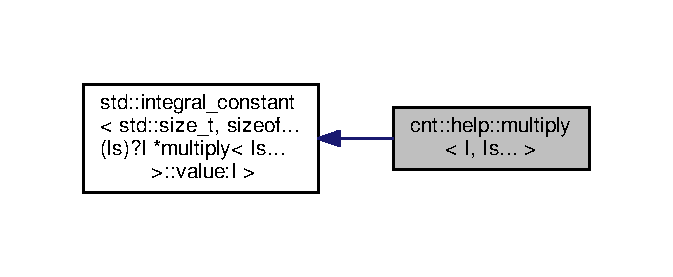
\includegraphics[width=323pt]{structcnt_1_1help_1_1multiply_3_01I_00_01Is_8_8_8_01_4__coll__graph}
\end{center}
\end{figure}


The documentation for this struct was generated from the following file\+:\begin{DoxyCompactItemize}
\item 
/home/matheus/\+Algoritmos/\+C\+P\+P/\+Handy/include/\+Container/\hyperlink{Container_2Helpers_8h}{Helpers.\+h}\end{DoxyCompactItemize}

\hypertarget{structcnt_1_1help_1_1multiply_3_4}{}\section{cnt\+:\+:help\+:\+:multiply$<$$>$ Struct Template Reference}
\label{structcnt_1_1help_1_1multiply_3_4}\index{cnt\+::help\+::multiply$<$$>$@{cnt\+::help\+::multiply$<$$>$}}


{\ttfamily \#include $<$Helpers.\+h$>$}



Inheritance diagram for cnt\+:\+:help\+:\+:multiply$<$$>$\+:\nopagebreak
\begin{figure}[H]
\begin{center}
\leavevmode
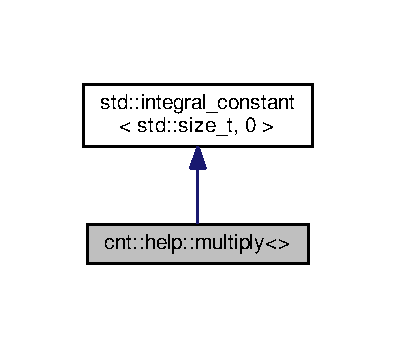
\includegraphics[width=190pt]{structcnt_1_1help_1_1multiply_3_4__inherit__graph}
\end{center}
\end{figure}


Collaboration diagram for cnt\+:\+:help\+:\+:multiply$<$$>$\+:\nopagebreak
\begin{figure}[H]
\begin{center}
\leavevmode
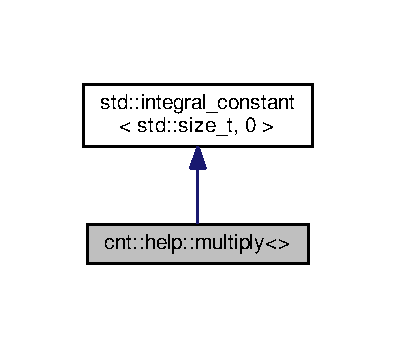
\includegraphics[width=190pt]{structcnt_1_1help_1_1multiply_3_4__coll__graph}
\end{center}
\end{figure}


The documentation for this struct was generated from the following file\+:\begin{DoxyCompactItemize}
\item 
/home/matheus/\+Algoritmos/\+C\+P\+P/\+Handy/include/\+Container/\hyperlink{Container_2Helpers_8h}{Helpers.\+h}\end{DoxyCompactItemize}

\hypertarget{structhandy_1_1impl_1_1RandBase}{}\section{handy\+:\+:impl\+:\+:Rand\+Base Struct Reference}
\label{structhandy_1_1impl_1_1RandBase}\index{handy\+::impl\+::\+Rand\+Base@{handy\+::impl\+::\+Rand\+Base}}


The base class for generating random numbers.  




{\ttfamily \#include $<$Random.\+h$>$}



Inheritance diagram for handy\+:\+:impl\+:\+:Rand\+Base\+:\nopagebreak
\begin{figure}[H]
\begin{center}
\leavevmode
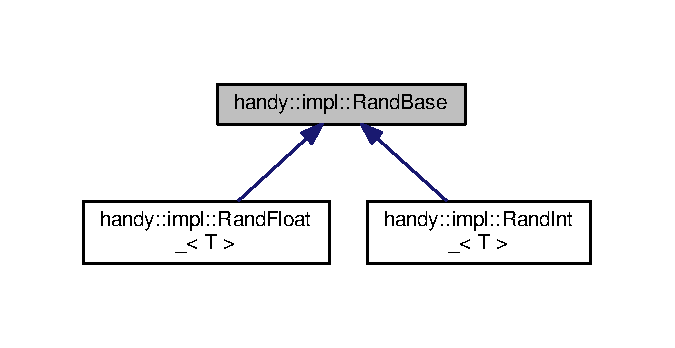
\includegraphics[width=324pt]{structhandy_1_1impl_1_1RandBase__inherit__graph}
\end{center}
\end{figure}


Collaboration diagram for handy\+:\+:impl\+:\+:Rand\+Base\+:\nopagebreak
\begin{figure}[H]
\begin{center}
\leavevmode
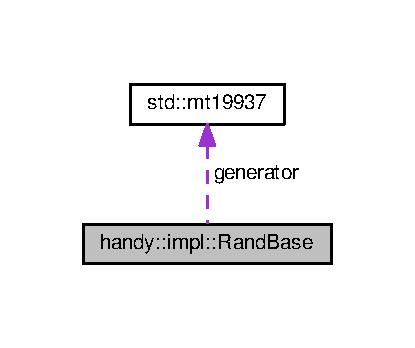
\includegraphics[width=199pt]{structhandy_1_1impl_1_1RandBase__coll__graph}
\end{center}
\end{figure}
\subsection*{Public Member Functions}
\begin{DoxyCompactItemize}
\item 
\hyperlink{group__RandomGroup_ga0ffb9e02dcdd71ed1fda48ca1e2f2fd5}{Rand\+Base} (unsigned int seed\+Val=-\/1)
\begin{DoxyCompactList}\small\item\em Default is \textquotesingle{}-\/1\textquotesingle{}. \end{DoxyCompactList}\item 
void \hyperlink{group__RandomGroup_ga3bb644a945c71368203459431818ddcd}{seed} (unsigned int seed\+Val=-\/1)
\begin{DoxyCompactList}\small\item\em Set a new seed value. \end{DoxyCompactList}\item 
unsigned int \hyperlink{group__RandomGroup_ga301c5bb729933e83eb5f071461169e9b}{pick\+Seed} (unsigned int seed\+Val)
\begin{DoxyCompactList}\small\item\em If {\ttfamily seed\+Val} is {\ttfamily -\/1}, pick the value given by {\bf std\+::random\+\_\+device}\{\}(). Otherwise, pick {\ttfamily seed\+Val}. \end{DoxyCompactList}\end{DoxyCompactItemize}
\subsection*{Public Attributes}
\begin{DoxyCompactItemize}
\item 
{\bf std\+::mt19937} \hyperlink{group__RandomGroup_gaecbff587706065e3d20a81de01123c9f}{generator}
\begin{DoxyCompactList}\small\item\em \hyperlink{}{Twister generator }\end{DoxyCompactList}\end{DoxyCompactItemize}


\subsection{Detailed Description}
The base class for generating random numbers. 

The class has only a generator variable (\hyperlink{group__RandomGroup_gaecbff587706065e3d20a81de01123c9f}{generator}) and a function for setting the seed value (\hyperlink{group__RandomGroup_ga3bb644a945c71368203459431818ddcd}{seed}) If you pass a {\ttfamily -\/1} (basically the same thing as {\bf std\+::string\+::max\+\_\+size()}), it will call {\bf std\+::random\+\_\+device}\{\}(), which will create the seed (pseudo-\/) randomly. 

The documentation for this struct was generated from the following file\+:\begin{DoxyCompactItemize}
\item 
/home/matheus/\+Algoritmos/\+C\+P\+P/\+Handy/include/\+Helpers/\hyperlink{Random_8h}{Random.\+h}\end{DoxyCompactItemize}

\hypertarget{structhandy_1_1impl_1_1RandFloat__}{}\section{handy\+:\+:impl\+:\+:Rand\+Float\+\_\+$<$ T $>$ Struct Template Reference}
\label{structhandy_1_1impl_1_1RandFloat__}\index{handy\+::impl\+::\+Rand\+Float\+\_\+$<$ T $>$@{handy\+::impl\+::\+Rand\+Float\+\_\+$<$ T $>$}}


For floating points.  




{\ttfamily \#include $<$Random.\+h$>$}



Inheritance diagram for handy\+:\+:impl\+:\+:Rand\+Float\+\_\+$<$ T $>$\+:\nopagebreak
\begin{figure}[H]
\begin{center}
\leavevmode
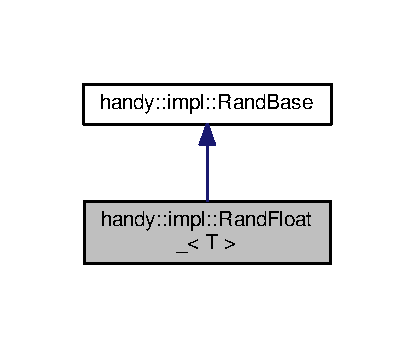
\includegraphics[width=199pt]{structhandy_1_1impl_1_1RandFloat____inherit__graph}
\end{center}
\end{figure}


Collaboration diagram for handy\+:\+:impl\+:\+:Rand\+Float\+\_\+$<$ T $>$\+:\nopagebreak
\begin{figure}[H]
\begin{center}
\leavevmode
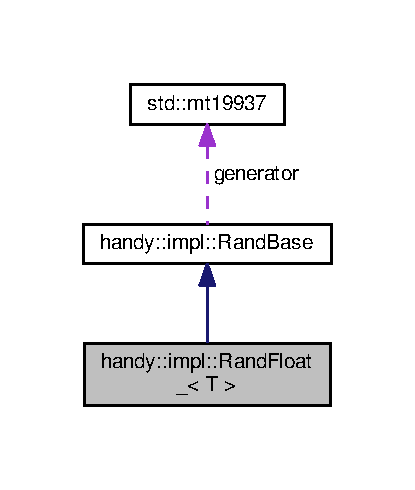
\includegraphics[width=199pt]{structhandy_1_1impl_1_1RandFloat____coll__graph}
\end{center}
\end{figure}
\subsection*{Public Member Functions}
\begin{DoxyCompactItemize}
\item 
T \hyperlink{group__RandomGroup_ga3448918864fd58b3dcbdad0c548323ce}{operator()} ()
\begin{DoxyCompactList}\small\item\em With no arguments, it will generate numbers between \mbox{[}0.\+0, 1.\+0) \end{DoxyCompactList}\item 
T \hyperlink{group__RandomGroup_ga8a3a1dc2369d8758d43250474a1c391d}{operator()} (T max)
\begin{DoxyCompactList}\small\item\em With a single argument, it will generate numbers between \mbox{[}0.\+0, max) \end{DoxyCompactList}\item 
T \hyperlink{group__RandomGroup_ga36eca80e7e43044caec35d03f27df419}{operator()} (T min, T max)
\begin{DoxyCompactList}\small\item\em Same as \textquotesingle{}\hyperlink{structhandy_1_1impl_1_1RandInt__}{Rand\+Int\+\_\+}\textquotesingle{}, but using a real uniform distribution now. It is also half closed \mbox{[}min, max). \end{DoxyCompactList}\end{DoxyCompactItemize}
\subsection*{Additional Inherited Members}


\subsection{Detailed Description}
\subsubsection*{template$<$typename T$>$\\*
struct handy\+::impl\+::\+Rand\+Float\+\_\+$<$ T $>$}

For floating points. 

The documentation for this struct was generated from the following file\+:\begin{DoxyCompactItemize}
\item 
/home/matheus/\+Algoritmos/\+C\+P\+P/\+Handy/include/\+Helpers/\hyperlink{Random_8h}{Random.\+h}\end{DoxyCompactItemize}

\hypertarget{structhandy_1_1impl_1_1RandInt__}{}\section{handy\+:\+:impl\+:\+:Rand\+Int\+\_\+$<$ T $>$ Struct Template Reference}
\label{structhandy_1_1impl_1_1RandInt__}\index{handy\+::impl\+::\+Rand\+Int\+\_\+$<$ T $>$@{handy\+::impl\+::\+Rand\+Int\+\_\+$<$ T $>$}}


For integer types only.  




{\ttfamily \#include $<$Random.\+h$>$}



Inheritance diagram for handy\+:\+:impl\+:\+:Rand\+Int\+\_\+$<$ T $>$\+:\nopagebreak
\begin{figure}[H]
\begin{center}
\leavevmode
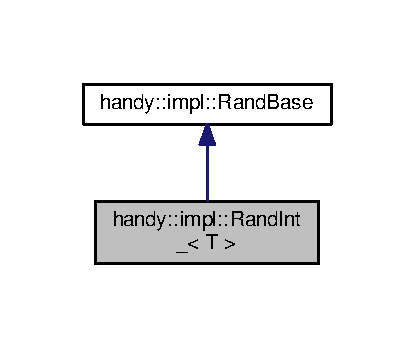
\includegraphics[width=199pt]{structhandy_1_1impl_1_1RandInt____inherit__graph}
\end{center}
\end{figure}


Collaboration diagram for handy\+:\+:impl\+:\+:Rand\+Int\+\_\+$<$ T $>$\+:\nopagebreak
\begin{figure}[H]
\begin{center}
\leavevmode
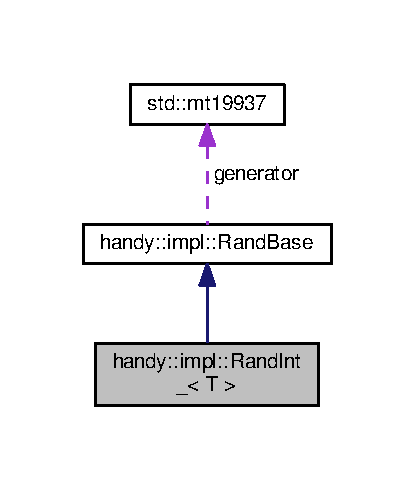
\includegraphics[width=199pt]{structhandy_1_1impl_1_1RandInt____coll__graph}
\end{center}
\end{figure}
\subsection*{Public Member Functions}
\begin{DoxyCompactItemize}
\item 
T \hyperlink{group__RandomGroup_gaf1314be58129341263aadf0e74ef44da}{operator()} ()
\begin{DoxyCompactList}\small\item\em With no arguments, it will generate numbers between \mbox{[}0, {\bf std\+::numeric\+\_\+limits$<$\+T$>$\+::max()}) \end{DoxyCompactList}\item 
T \hyperlink{group__RandomGroup_gae6a2e95b745f7e9f9fadee0e9bab54f9}{operator()} (T max)
\begin{DoxyCompactList}\small\item\em With a single argument, it will generate numbers between \mbox{[}0, max) \end{DoxyCompactList}\item 
T \hyperlink{group__RandomGroup_gaae84dc62705bd77108f258555fa89925}{operator()} (T min, T max)
\begin{DoxyCompactList}\small\item\em The generating function, which takes a {\ttfamily min} and {\ttfamily max} values, and uses \hyperlink{group__RandomGroup_gaecbff587706065e3d20a81de01123c9f}{handy\+::impl\+::\+Rand\+Base\+::generator()} \end{DoxyCompactList}\end{DoxyCompactItemize}
\subsection*{Additional Inherited Members}


\subsection{Detailed Description}
\subsubsection*{template$<$typename T$>$\\*
struct handy\+::impl\+::\+Rand\+Int\+\_\+$<$ T $>$}

For integer types only. 

The documentation for this struct was generated from the following file\+:\begin{DoxyCompactItemize}
\item 
/home/matheus/\+Algoritmos/\+C\+P\+P/\+Handy/include/\+Helpers/\hyperlink{Random_8h}{Random.\+h}\end{DoxyCompactItemize}

\hypertarget{classhandy_1_1Range}{}\section{handy\+:\+:Range$<$ T, Valid\+Range $>$ Class Template Reference}
\label{classhandy_1_1Range}\index{handy\+::\+Range$<$ T, Valid\+Range $>$@{handy\+::\+Range$<$ T, Valid\+Range $>$}}


{\ttfamily \#include $<$Range.\+h$>$}

\subsection*{Classes}
\begin{DoxyCompactItemize}
\item 
class \hyperlink{classhandy_1_1Range_1_1Iterator}{Iterator}
\end{DoxyCompactItemize}
\subsection*{Public Types}
\begin{DoxyCompactItemize}
\item 
using \hyperlink{classhandy_1_1Range_a2a8c2d169657c93464989e7608ed3f9b}{Type} = std\+::decay\+\_\+t$<$ T $>$
\item 
using \hyperlink{classhandy_1_1Range_ab2b8b141ea04ed06e53938c899b5fa8a}{value\+\_\+type} = \hyperlink{classhandy_1_1Range_a2a8c2d169657c93464989e7608ed3f9b}{Type}
\item 
using \hyperlink{classhandy_1_1Range_ad879bbe314ce7bcffdda15a0f065e0f8}{iterator} = \hyperlink{classhandy_1_1Range_1_1Iterator}{Iterator}
\item 
using \hyperlink{classhandy_1_1Range_a9d4a18bcffddb19f6dcc2d9088fd5219}{iterator\+\_\+category} = typename \hyperlink{classhandy_1_1Range_1_1Iterator_a5e9da733ea7dadc2cc69327288e3e7a2}{iterator\+::iterator\+\_\+category}
\item 
using \hyperlink{classhandy_1_1Range_a776521ae1ca6a10d1be256ecdf26f6e2}{const\+\_\+iterator} = \hyperlink{classhandy_1_1Range_ad879bbe314ce7bcffdda15a0f065e0f8}{iterator}
\end{DoxyCompactItemize}
\subsection*{Public Member Functions}
\begin{DoxyCompactItemize}
\item 
\hyperlink{classhandy_1_1Range_ac75e53eb61792ac1a682d51913633709}{Range} (const \hyperlink{classhandy_1_1Range_a2a8c2d169657c93464989e7608ed3f9b}{Type} \&last)
\item 
\hyperlink{classhandy_1_1Range_a9496d5be63390d116e8ac513941ad805}{Range} (const \hyperlink{classhandy_1_1Range_a2a8c2d169657c93464989e7608ed3f9b}{Type} \&first, const \hyperlink{classhandy_1_1Range_a2a8c2d169657c93464989e7608ed3f9b}{Type} \&last)
\item 
\hyperlink{classhandy_1_1Range_a6e6f90cfac8ae3c265c82d25e01bd0ba}{Range} (const \hyperlink{classhandy_1_1Range_a2a8c2d169657c93464989e7608ed3f9b}{Type} \&first, const \hyperlink{classhandy_1_1Range_a2a8c2d169657c93464989e7608ed3f9b}{Type} \&last, const \hyperlink{classhandy_1_1Range_a2a8c2d169657c93464989e7608ed3f9b}{Type} \&step)
\item 
\hyperlink{classhandy_1_1Range_ad879bbe314ce7bcffdda15a0f065e0f8}{iterator} \hyperlink{classhandy_1_1Range_ae6142e67b348d891966b97671acb890a}{begin} ()
\item 
\hyperlink{classhandy_1_1Range_ad879bbe314ce7bcffdda15a0f065e0f8}{iterator} \hyperlink{classhandy_1_1Range_a423264a5e77f59b8a47739e5d47f5e81}{end} ()
\item 
\hyperlink{classhandy_1_1Range_a776521ae1ca6a10d1be256ecdf26f6e2}{const\+\_\+iterator} \hyperlink{classhandy_1_1Range_a3e3e4186610dd72a275881e597285b8b}{begin} () const 
\item 
\hyperlink{classhandy_1_1Range_a776521ae1ca6a10d1be256ecdf26f6e2}{const\+\_\+iterator} \hyperlink{classhandy_1_1Range_a69e9c4ca833c91459594e71d3f83c3e8}{end} () const 
\item 
{\bf std\+::vector}$<$ \hyperlink{classhandy_1_1Range_a2a8c2d169657c93464989e7608ed3f9b}{Type} $>$ \hyperlink{classhandy_1_1Range_a7a0457913f0bc3698b6172910ca5070b}{eval} ()
\item 
{\footnotesize template$<$typename Iter $>$ }\\void \hyperlink{classhandy_1_1Range_aedef8b41234dd9832701619696fcd239}{eval} (Iter iter)
\end{DoxyCompactItemize}
\subsection*{Public Attributes}
\begin{DoxyCompactItemize}
\item 
friend \hyperlink{classhandy_1_1Range_a65634287fdb689e410c0c4af5bb2ec05}{Iterator}
\end{DoxyCompactItemize}


\subsection{Member Typedef Documentation}
\index{handy\+::\+Range@{handy\+::\+Range}!const\+\_\+iterator@{const\+\_\+iterator}}
\index{const\+\_\+iterator@{const\+\_\+iterator}!handy\+::\+Range@{handy\+::\+Range}}
\subsubsection[{\texorpdfstring{const\+\_\+iterator}{const_iterator}}]{\setlength{\rightskip}{0pt plus 5cm}template$<$typename T, typename Valid\+Range = impl\+::\+Half\+Closed\+Interval$>$ using {\bf handy\+::\+Range}$<$ T, Valid\+Range $>$\+::{\bf const\+\_\+iterator} =  {\bf iterator}}\hypertarget{classhandy_1_1Range_a776521ae1ca6a10d1be256ecdf26f6e2}{}\label{classhandy_1_1Range_a776521ae1ca6a10d1be256ecdf26f6e2}
You will never use \textquotesingle{}const Iterator$<$t$>$\textquotesingle{} in pratice. But, if you do, the iterator cannot really be const, so we can increment the \textquotesingle{}value\textquotesingle{} variable. \index{handy\+::\+Range@{handy\+::\+Range}!iterator@{iterator}}
\index{iterator@{iterator}!handy\+::\+Range@{handy\+::\+Range}}
\subsubsection[{\texorpdfstring{iterator}{iterator}}]{\setlength{\rightskip}{0pt plus 5cm}template$<$typename T, typename Valid\+Range = impl\+::\+Half\+Closed\+Interval$>$ using {\bf handy\+::\+Range}$<$ T, Valid\+Range $>$\+::{\bf iterator} =  {\bf Iterator}}\hypertarget{classhandy_1_1Range_ad879bbe314ce7bcffdda15a0f065e0f8}{}\label{classhandy_1_1Range_ad879bbe314ce7bcffdda15a0f065e0f8}
\index{handy\+::\+Range@{handy\+::\+Range}!iterator\+\_\+category@{iterator\+\_\+category}}
\index{iterator\+\_\+category@{iterator\+\_\+category}!handy\+::\+Range@{handy\+::\+Range}}
\subsubsection[{\texorpdfstring{iterator\+\_\+category}{iterator_category}}]{\setlength{\rightskip}{0pt plus 5cm}template$<$typename T, typename Valid\+Range = impl\+::\+Half\+Closed\+Interval$>$ using {\bf handy\+::\+Range}$<$ T, Valid\+Range $>$\+::{\bf iterator\+\_\+category} =  typename {\bf iterator\+::iterator\+\_\+category}}\hypertarget{classhandy_1_1Range_a9d4a18bcffddb19f6dcc2d9088fd5219}{}\label{classhandy_1_1Range_a9d4a18bcffddb19f6dcc2d9088fd5219}
\index{handy\+::\+Range@{handy\+::\+Range}!Type@{Type}}
\index{Type@{Type}!handy\+::\+Range@{handy\+::\+Range}}
\subsubsection[{\texorpdfstring{Type}{Type}}]{\setlength{\rightskip}{0pt plus 5cm}template$<$typename T, typename Valid\+Range = impl\+::\+Half\+Closed\+Interval$>$ using {\bf handy\+::\+Range}$<$ T, Valid\+Range $>$\+::{\bf Type} =  std\+::decay\+\_\+t$<$T$>$}\hypertarget{classhandy_1_1Range_a2a8c2d169657c93464989e7608ed3f9b}{}\label{classhandy_1_1Range_a2a8c2d169657c93464989e7608ed3f9b}
\index{handy\+::\+Range@{handy\+::\+Range}!value\+\_\+type@{value\+\_\+type}}
\index{value\+\_\+type@{value\+\_\+type}!handy\+::\+Range@{handy\+::\+Range}}
\subsubsection[{\texorpdfstring{value\+\_\+type}{value_type}}]{\setlength{\rightskip}{0pt plus 5cm}template$<$typename T, typename Valid\+Range = impl\+::\+Half\+Closed\+Interval$>$ using {\bf handy\+::\+Range}$<$ T, Valid\+Range $>$\+::{\bf value\+\_\+type} =  {\bf Type}}\hypertarget{classhandy_1_1Range_ab2b8b141ea04ed06e53938c899b5fa8a}{}\label{classhandy_1_1Range_ab2b8b141ea04ed06e53938c899b5fa8a}


\subsection{Constructor \& Destructor Documentation}
\index{handy\+::\+Range@{handy\+::\+Range}!Range@{Range}}
\index{Range@{Range}!handy\+::\+Range@{handy\+::\+Range}}
\subsubsection[{\texorpdfstring{Range(const Type \&last)}{Range(const Type &last)}}]{\setlength{\rightskip}{0pt plus 5cm}template$<$typename T, typename Valid\+Range = impl\+::\+Half\+Closed\+Interval$>$ {\bf handy\+::\+Range}$<$ T, Valid\+Range $>$\+::{\bf Range} (
\begin{DoxyParamCaption}
\item[{const {\bf Type} \&}]{last}
\end{DoxyParamCaption}
)\hspace{0.3cm}{\ttfamily [inline]}}\hypertarget{classhandy_1_1Range_ac75e53eb61792ac1a682d51913633709}{}\label{classhandy_1_1Range_ac75e53eb61792ac1a682d51913633709}
\index{handy\+::\+Range@{handy\+::\+Range}!Range@{Range}}
\index{Range@{Range}!handy\+::\+Range@{handy\+::\+Range}}
\subsubsection[{\texorpdfstring{Range(const Type \&first, const Type \&last)}{Range(const Type &first, const Type &last)}}]{\setlength{\rightskip}{0pt plus 5cm}template$<$typename T, typename Valid\+Range = impl\+::\+Half\+Closed\+Interval$>$ {\bf handy\+::\+Range}$<$ T, Valid\+Range $>$\+::{\bf Range} (
\begin{DoxyParamCaption}
\item[{const {\bf Type} \&}]{first, }
\item[{const {\bf Type} \&}]{last}
\end{DoxyParamCaption}
)\hspace{0.3cm}{\ttfamily [inline]}}\hypertarget{classhandy_1_1Range_a9496d5be63390d116e8ac513941ad805}{}\label{classhandy_1_1Range_a9496d5be63390d116e8ac513941ad805}
\index{handy\+::\+Range@{handy\+::\+Range}!Range@{Range}}
\index{Range@{Range}!handy\+::\+Range@{handy\+::\+Range}}
\subsubsection[{\texorpdfstring{Range(const Type \&first, const Type \&last, const Type \&step)}{Range(const Type &first, const Type &last, const Type &step)}}]{\setlength{\rightskip}{0pt plus 5cm}template$<$typename T, typename Valid\+Range = impl\+::\+Half\+Closed\+Interval$>$ {\bf handy\+::\+Range}$<$ T, Valid\+Range $>$\+::{\bf Range} (
\begin{DoxyParamCaption}
\item[{const {\bf Type} \&}]{first, }
\item[{const {\bf Type} \&}]{last, }
\item[{const {\bf Type} \&}]{step}
\end{DoxyParamCaption}
)\hspace{0.3cm}{\ttfamily [inline]}}\hypertarget{classhandy_1_1Range_a6e6f90cfac8ae3c265c82d25e01bd0ba}{}\label{classhandy_1_1Range_a6e6f90cfac8ae3c265c82d25e01bd0ba}
To be a valid range, there must be a positive number \textquotesingle{}c\textquotesingle{} such that\+:

first + c $\ast$ step = last ---$>$ c = (last -\/ first) / step

As we only care for the sign of \textquotesingle{}c\textquotesingle{}, we can change the division by a multiplication. The equal test is for the case where \textquotesingle{}last == first\textquotesingle{}.

\subsection{Member Function Documentation}
\index{handy\+::\+Range@{handy\+::\+Range}!begin@{begin}}
\index{begin@{begin}!handy\+::\+Range@{handy\+::\+Range}}
\subsubsection[{\texorpdfstring{begin()}{begin()}}]{\setlength{\rightskip}{0pt plus 5cm}template$<$typename T, typename Valid\+Range = impl\+::\+Half\+Closed\+Interval$>$ {\bf iterator} {\bf handy\+::\+Range}$<$ T, Valid\+Range $>$\+::begin (
\begin{DoxyParamCaption}
{}
\end{DoxyParamCaption}
)\hspace{0.3cm}{\ttfamily [inline]}}\hypertarget{classhandy_1_1Range_ae6142e67b348d891966b97671acb890a}{}\label{classhandy_1_1Range_ae6142e67b348d891966b97671acb890a}
\index{handy\+::\+Range@{handy\+::\+Range}!begin@{begin}}
\index{begin@{begin}!handy\+::\+Range@{handy\+::\+Range}}
\subsubsection[{\texorpdfstring{begin() const }{begin() const }}]{\setlength{\rightskip}{0pt plus 5cm}template$<$typename T, typename Valid\+Range = impl\+::\+Half\+Closed\+Interval$>$ {\bf const\+\_\+iterator} {\bf handy\+::\+Range}$<$ T, Valid\+Range $>$\+::begin (
\begin{DoxyParamCaption}
{}
\end{DoxyParamCaption}
) const\hspace{0.3cm}{\ttfamily [inline]}}\hypertarget{classhandy_1_1Range_a3e3e4186610dd72a275881e597285b8b}{}\label{classhandy_1_1Range_a3e3e4186610dd72a275881e597285b8b}
\index{handy\+::\+Range@{handy\+::\+Range}!end@{end}}
\index{end@{end}!handy\+::\+Range@{handy\+::\+Range}}
\subsubsection[{\texorpdfstring{end()}{end()}}]{\setlength{\rightskip}{0pt plus 5cm}template$<$typename T, typename Valid\+Range = impl\+::\+Half\+Closed\+Interval$>$ {\bf iterator} {\bf handy\+::\+Range}$<$ T, Valid\+Range $>$\+::end (
\begin{DoxyParamCaption}
{}
\end{DoxyParamCaption}
)\hspace{0.3cm}{\ttfamily [inline]}}\hypertarget{classhandy_1_1Range_a423264a5e77f59b8a47739e5d47f5e81}{}\label{classhandy_1_1Range_a423264a5e77f59b8a47739e5d47f5e81}
\index{handy\+::\+Range@{handy\+::\+Range}!end@{end}}
\index{end@{end}!handy\+::\+Range@{handy\+::\+Range}}
\subsubsection[{\texorpdfstring{end() const }{end() const }}]{\setlength{\rightskip}{0pt plus 5cm}template$<$typename T, typename Valid\+Range = impl\+::\+Half\+Closed\+Interval$>$ {\bf const\+\_\+iterator} {\bf handy\+::\+Range}$<$ T, Valid\+Range $>$\+::end (
\begin{DoxyParamCaption}
{}
\end{DoxyParamCaption}
) const\hspace{0.3cm}{\ttfamily [inline]}}\hypertarget{classhandy_1_1Range_a69e9c4ca833c91459594e71d3f83c3e8}{}\label{classhandy_1_1Range_a69e9c4ca833c91459594e71d3f83c3e8}
\index{handy\+::\+Range@{handy\+::\+Range}!eval@{eval}}
\index{eval@{eval}!handy\+::\+Range@{handy\+::\+Range}}
\subsubsection[{\texorpdfstring{eval()}{eval()}}]{\setlength{\rightskip}{0pt plus 5cm}template$<$typename T, typename Valid\+Range = impl\+::\+Half\+Closed\+Interval$>$ {\bf std\+::vector}$<${\bf Type}$>$ {\bf handy\+::\+Range}$<$ T, Valid\+Range $>$\+::eval (
\begin{DoxyParamCaption}
{}
\end{DoxyParamCaption}
)\hspace{0.3cm}{\ttfamily [inline]}}\hypertarget{classhandy_1_1Range_a7a0457913f0bc3698b6172910ca5070b}{}\label{classhandy_1_1Range_a7a0457913f0bc3698b6172910ca5070b}
\index{handy\+::\+Range@{handy\+::\+Range}!eval@{eval}}
\index{eval@{eval}!handy\+::\+Range@{handy\+::\+Range}}
\subsubsection[{\texorpdfstring{eval(\+Iter iter)}{eval(Iter iter)}}]{\setlength{\rightskip}{0pt plus 5cm}template$<$typename T, typename Valid\+Range = impl\+::\+Half\+Closed\+Interval$>$ template$<$typename Iter $>$ void {\bf handy\+::\+Range}$<$ T, Valid\+Range $>$\+::eval (
\begin{DoxyParamCaption}
\item[{Iter}]{iter}
\end{DoxyParamCaption}
)\hspace{0.3cm}{\ttfamily [inline]}}\hypertarget{classhandy_1_1Range_aedef8b41234dd9832701619696fcd239}{}\label{classhandy_1_1Range_aedef8b41234dd9832701619696fcd239}


\subsection{Member Data Documentation}
\index{handy\+::\+Range@{handy\+::\+Range}!Iterator@{Iterator}}
\index{Iterator@{Iterator}!handy\+::\+Range@{handy\+::\+Range}}
\subsubsection[{\texorpdfstring{Iterator}{Iterator}}]{\setlength{\rightskip}{0pt plus 5cm}template$<$typename T, typename Valid\+Range = impl\+::\+Half\+Closed\+Interval$>$ friend {\bf handy\+::\+Range}$<$ T, Valid\+Range $>$\+::{\bf Iterator}}\hypertarget{classhandy_1_1Range_a65634287fdb689e410c0c4af5bb2ec05}{}\label{classhandy_1_1Range_a65634287fdb689e410c0c4af5bb2ec05}


The documentation for this class was generated from the following file\+:\begin{DoxyCompactItemize}
\item 
/home/matheus/\+Algoritmos/\+C\+P\+P/\+Handy/include/\+Range/\hyperlink{Range_8h}{Range.\+h}\end{DoxyCompactItemize}

\hypertarget{structit_1_1help_1_1SelectIterTag}{}\section{it\+:\+:help\+:\+:Select\+Iter\+Tag$<$... $>$ Struct Template Reference}
\label{structit_1_1help_1_1SelectIterTag}\index{it\+::help\+::\+Select\+Iter\+Tag$<$... $>$@{it\+::help\+::\+Select\+Iter\+Tag$<$... $>$}}


Selects the smallest (the more generic) iterator type from an variadic argument list.  




{\ttfamily \#include $<$Helpers.\+h$>$}



\subsection{Detailed Description}
\subsubsection*{template$<$class...$>$\\*
struct it\+::help\+::\+Select\+Iter\+Tag$<$... $>$}

Selects the smallest (the more generic) iterator type from an variadic argument list. 

The documentation for this struct was generated from the following file\+:\begin{DoxyCompactItemize}
\item 
/home/matheus/\+Algoritmos/\+C\+P\+P/\+Handy/include/\+Zip\+Iter/\hyperlink{ZipIter_2Helpers_8h}{Helpers.\+h}\end{DoxyCompactItemize}

\hypertarget{structit_1_1help_1_1SelectIterTag_3_01Iter_01_4}{}\section{it\+:\+:help\+:\+:Select\+Iter\+Tag$<$ Iter $>$ Struct Template Reference}
\label{structit_1_1help_1_1SelectIterTag_3_01Iter_01_4}\index{it\+::help\+::\+Select\+Iter\+Tag$<$ Iter $>$@{it\+::help\+::\+Select\+Iter\+Tag$<$ Iter $>$}}


{\ttfamily \#include $<$Helpers.\+h$>$}

\subsection*{Public Types}
\begin{DoxyCompactItemize}
\item 
using \hyperlink{structit_1_1help_1_1SelectIterTag_3_01Iter_01_4_a7357cce64ed4c2e4a225b4dce5a5341d}{type} = Iter
\end{DoxyCompactItemize}


\subsection{Member Typedef Documentation}
\index{it\+::help\+::\+Select\+Iter\+Tag$<$ Iter $>$@{it\+::help\+::\+Select\+Iter\+Tag$<$ Iter $>$}!type@{type}}
\index{type@{type}!it\+::help\+::\+Select\+Iter\+Tag$<$ Iter $>$@{it\+::help\+::\+Select\+Iter\+Tag$<$ Iter $>$}}
\subsubsection[{\texorpdfstring{type}{type}}]{\setlength{\rightskip}{0pt plus 5cm}template$<$class Iter $>$ using {\bf it\+::help\+::\+Select\+Iter\+Tag}$<$ Iter $>$\+::{\bf type} =  Iter}\hypertarget{structit_1_1help_1_1SelectIterTag_3_01Iter_01_4_a7357cce64ed4c2e4a225b4dce5a5341d}{}\label{structit_1_1help_1_1SelectIterTag_3_01Iter_01_4_a7357cce64ed4c2e4a225b4dce5a5341d}


The documentation for this struct was generated from the following file\+:\begin{DoxyCompactItemize}
\item 
/home/matheus/\+Algoritmos/\+C\+P\+P/\+Handy/include/\+Zip\+Iter/\hyperlink{ZipIter_2Helpers_8h}{Helpers.\+h}\end{DoxyCompactItemize}

\hypertarget{structit_1_1help_1_1SelectIterTag_3_01Iter_00_01Iters_8_8_8_01_4}{}\section{it\+:\+:help\+:\+:Select\+Iter\+Tag$<$ Iter, Iters... $>$ Struct Template Reference}
\label{structit_1_1help_1_1SelectIterTag_3_01Iter_00_01Iters_8_8_8_01_4}\index{it\+::help\+::\+Select\+Iter\+Tag$<$ Iter, Iters... $>$@{it\+::help\+::\+Select\+Iter\+Tag$<$ Iter, Iters... $>$}}


{\ttfamily \#include $<$Helpers.\+h$>$}



Inheritance diagram for it\+:\+:help\+:\+:Select\+Iter\+Tag$<$ Iter, Iters... $>$\+:\nopagebreak
\begin{figure}[H]
\begin{center}
\leavevmode
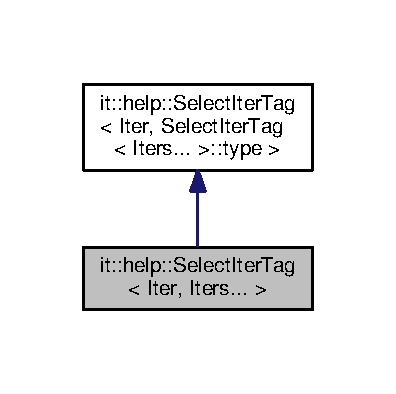
\includegraphics[width=190pt]{structit_1_1help_1_1SelectIterTag_3_01Iter_00_01Iters_8_8_8_01_4__inherit__graph}
\end{center}
\end{figure}


Collaboration diagram for it\+:\+:help\+:\+:Select\+Iter\+Tag$<$ Iter, Iters... $>$\+:\nopagebreak
\begin{figure}[H]
\begin{center}
\leavevmode
\includegraphics[width=190pt]{structit_1_1help_1_1SelectIterTag_3_01Iter_00_01Iters_8_8_8_01_4__coll__graph}
\end{center}
\end{figure}


The documentation for this struct was generated from the following file\+:\begin{DoxyCompactItemize}
\item 
/home/matheus/\+Algoritmos/\+C\+P\+P/\+Handy/include/\+Zip\+Iter/\hyperlink{ZipIter_2Helpers_8h}{Helpers.\+h}\end{DoxyCompactItemize}

\hypertarget{structit_1_1help_1_1SelectIterTag_3_01Iter1_00_01Iter2_01_4}{}\section{it\+:\+:help\+:\+:Select\+Iter\+Tag$<$ Iter1, Iter2 $>$ Struct Template Reference}
\label{structit_1_1help_1_1SelectIterTag_3_01Iter1_00_01Iter2_01_4}\index{it\+::help\+::\+Select\+Iter\+Tag$<$ Iter1, Iter2 $>$@{it\+::help\+::\+Select\+Iter\+Tag$<$ Iter1, Iter2 $>$}}


{\ttfamily \#include $<$Helpers.\+h$>$}

\subsection*{Public Types}
\begin{DoxyCompactItemize}
\item 
using \hyperlink{structit_1_1help_1_1SelectIterTag_3_01Iter1_00_01Iter2_01_4_ab9e5a0f79cab82e1c16f3a4a38029df9}{type} = std\+::conditional\+\_\+t$<$ (\hyperlink{namespaceit_1_1help_ad5efd6f9a3703da509d0853b95b515db}{iter\+Tag\+Order}(Iter1\{\})$<$ \hyperlink{namespaceit_1_1help_ad5efd6f9a3703da509d0853b95b515db}{iter\+Tag\+Order}(Iter2\{\})), Iter1, Iter2 $>$
\end{DoxyCompactItemize}


\subsection{Member Typedef Documentation}
\index{it\+::help\+::\+Select\+Iter\+Tag$<$ Iter1, Iter2 $>$@{it\+::help\+::\+Select\+Iter\+Tag$<$ Iter1, Iter2 $>$}!type@{type}}
\index{type@{type}!it\+::help\+::\+Select\+Iter\+Tag$<$ Iter1, Iter2 $>$@{it\+::help\+::\+Select\+Iter\+Tag$<$ Iter1, Iter2 $>$}}
\subsubsection[{\texorpdfstring{type}{type}}]{\setlength{\rightskip}{0pt plus 5cm}template$<$class Iter1 , class Iter2 $>$ using {\bf it\+::help\+::\+Select\+Iter\+Tag}$<$ Iter1, Iter2 $>$\+::{\bf type} =  std\+::conditional\+\_\+t$<$ ({\bf iter\+Tag\+Order}(Iter1\{\}) $<$ {\bf iter\+Tag\+Order}(Iter2\{\})), Iter1, Iter2 $>$}\hypertarget{structit_1_1help_1_1SelectIterTag_3_01Iter1_00_01Iter2_01_4_ab9e5a0f79cab82e1c16f3a4a38029df9}{}\label{structit_1_1help_1_1SelectIterTag_3_01Iter1_00_01Iter2_01_4_ab9e5a0f79cab82e1c16f3a4a38029df9}


The documentation for this struct was generated from the following file\+:\begin{DoxyCompactItemize}
\item 
/home/matheus/\+Algoritmos/\+C\+P\+P/\+Handy/include/\+Zip\+Iter/\hyperlink{ZipIter_2Helpers_8h}{Helpers.\+h}\end{DoxyCompactItemize}

\hypertarget{classcnt_1_1help_1_1Slice}{}\section{cnt\+:\+:help\+:\+:Slice$<$ Cnt $>$ Class Template Reference}
\label{classcnt_1_1help_1_1Slice}\index{cnt\+::help\+::\+Slice$<$ Cnt $>$@{cnt\+::help\+::\+Slice$<$ Cnt $>$}}


{\ttfamily \#include $<$Slice.\+h$>$}

\subsection*{Public Types}
{\bf }\par
\begin{DoxyCompactItemize}
\item 
using \hyperlink{classcnt_1_1help_1_1Slice_a485438785457de81fe42a4b07ec4ad32}{Base} = std\+::decay\+\_\+t$<$ Cnt $>$
\item 
using \hyperlink{classcnt_1_1help_1_1Slice_a7d0f8ecb603e485ce53f12cce307821d}{value\+\_\+type} = typename Base\+::value\+\_\+type
\item 
using \hyperlink{classcnt_1_1help_1_1Slice_a5e5e9b497c124710fcfe1e185e4801f3}{reference} = typename Base\+::reference
\item 
using \hyperlink{classcnt_1_1help_1_1Slice_aed38e8e92115049f9c3b78ee67bdc5c4}{const\+\_\+reference} = typename Base\+::const\+\_\+reference
\end{DoxyCompactItemize}

\subsection*{Public Member Functions}
\begin{DoxyCompactItemize}
\item 
auto \hyperlink{classcnt_1_1help_1_1Slice_a0357feeda100757b1202ee9e24021ed0}{size} (int p) const 
\begin{DoxyCompactList}\small\item\em Size of each dimension. \end{DoxyCompactList}\item 
auto \hyperlink{classcnt_1_1help_1_1Slice_ae3af5fdf7436c2de291611e68495b471}{size} () const 
\begin{DoxyCompactList}\small\item\em Total size of the slice. \end{DoxyCompactList}\end{DoxyCompactItemize}
{\bf }\par
\begin{DoxyCompactItemize}
\item 
{\footnotesize template$<$typename... Args, help\+::\+Enable\+If\+Integral$<$ std\+::decay\+\_\+t$<$ Args $>$... $>$  = 0$>$ }\\\hyperlink{classcnt_1_1help_1_1Slice_a4ee48993f74932456f8bc49790bd0c6f}{Slice} (Cnt \&c, const Args \&...args)
\begin{DoxyCompactList}\small\item\em For integrals. \end{DoxyCompactList}\item 
{\footnotesize template$<$typename... Args, std\+::enable\+\_\+if\+\_\+t$<$ sizeof...(\+Args), int $>$  = 0, help\+::\+Enable\+If\+Iterable$<$ std\+::remove\+\_\+reference\+\_\+t$<$ Args $>$... $>$  = 0$>$ }\\\hyperlink{classcnt_1_1help_1_1Slice_ad48e78da8f37d92bb4f9a8a913270cfe}{Slice} (Cnt \&c, const Args \&...args)
\begin{DoxyCompactList}\small\item\em For iterables. \end{DoxyCompactList}\item 
{\footnotesize template$<$typename U , typename V , help\+::\+Enable\+If\+Iterator$<$ std\+::decay\+\_\+t$<$ U $>$, std\+::decay\+\_\+t$<$ V $>$ $>$  = 0$>$ }\\\hyperlink{classcnt_1_1help_1_1Slice_a4691d18fed41988537d2bab287cb540b}{Slice} (Cnt \&c, const U \&\hyperlink{classcnt_1_1help_1_1Slice_aa5686f75940716e2568165e3b88d89d3}{begin}, const V \&\hyperlink{classcnt_1_1help_1_1Slice_a0bebfdc0b631e2462b54b2bd44059b76}{end})
\begin{DoxyCompactList}\small\item\em For a range defined by iterators. \end{DoxyCompactList}\item 
{\footnotesize template$<$typename U , help\+::\+Enable\+If\+Integral$<$ std\+::decay\+\_\+t$<$ U $>$$>$  = 0$>$ }\\\hyperlink{classcnt_1_1help_1_1Slice_a9ff9b2280e91eddd2b4e7f342f84aead}{Slice} (Cnt \&c, {\bf std\+::initializer\+\_\+list}$<$ U $>$ il)
\begin{DoxyCompactList}\small\item\em For list initialization. \end{DoxyCompactList}\end{DoxyCompactItemize}

{\bf }\par
\begin{DoxyCompactItemize}
\item 
{\footnotesize template$<$typename... Args$>$ }\\\hyperlink{classcnt_1_1help_1_1Slice_aed38e8e92115049f9c3b78ee67bdc5c4}{const\+\_\+reference} \hyperlink{classcnt_1_1help_1_1Slice_a5f6ebc78fcb07cb04aed2707e83efd92}{operator()} (\hyperlink{structcnt_1_1help_1_1IntegralType}{Integral\+Type}, const Args \&...args) const 
\begin{DoxyCompactList}\small\item\em For integral or iterable types. \end{DoxyCompactList}\item 
{\footnotesize template$<$typename U , help\+::\+Enable\+If\+Iterator$<$ std\+::decay\+\_\+t$<$ U $>$$>$  = 0$>$ }\\\hyperlink{classcnt_1_1help_1_1Slice_aed38e8e92115049f9c3b78ee67bdc5c4}{const\+\_\+reference} \hyperlink{classcnt_1_1help_1_1Slice_a28aad2a3fb6704596e1a317add0e3477}{operator()} (\hyperlink{structcnt_1_1help_1_1IteratorType}{Iterator\+Type}, const U \&\hyperlink{classcnt_1_1help_1_1Slice_aa5686f75940716e2568165e3b88d89d3}{begin}) const 
\begin{DoxyCompactList}\small\item\em For iterators. \end{DoxyCompactList}\item 
{\footnotesize template$<$typename U $>$ }\\\hyperlink{classcnt_1_1help_1_1Slice_aed38e8e92115049f9c3b78ee67bdc5c4}{const\+\_\+reference} \hyperlink{classcnt_1_1help_1_1Slice_a0263b9218c9f281b737dd9231f9c43e7}{operator()} ({\bf std\+::initializer\+\_\+list}$<$ U $>$ il) const 
\begin{DoxyCompactList}\small\item\em For \textquotesingle{}std\+::intializer\+\_\+lists\textquotesingle{}. \end{DoxyCompactList}\item 
\hyperlink{classcnt_1_1help_1_1Slice_aed38e8e92115049f9c3b78ee67bdc5c4}{const\+\_\+reference} \hyperlink{classcnt_1_1help_1_1Slice_a01908e8f74cf4a2a4d69ee8ad5f1a431}{operator\mbox{[}$\,$\mbox{]}} (int p) const 
\item 
\hyperlink{classcnt_1_1help_1_1Slice_a5e5e9b497c124710fcfe1e185e4801f3}{reference} \hyperlink{classcnt_1_1help_1_1Slice_a8eaabe725363ef76a42c15aadf7baa50}{operator\mbox{[}$\,$\mbox{]}} (int p)
\end{DoxyCompactItemize}

{\bf }\par
\begin{DoxyCompactItemize}
\item 
decltype(auto) \hyperlink{classcnt_1_1help_1_1Slice_aa5686f75940716e2568165e3b88d89d3}{begin} ()
\item 
decltype(auto) \hyperlink{classcnt_1_1help_1_1Slice_a8c37189a46abc4b6e5d3bbe19d070def}{cbegin} () const 
\item 
decltype(auto) \hyperlink{classcnt_1_1help_1_1Slice_a0bebfdc0b631e2462b54b2bd44059b76}{end} ()
\item 
decltype(auto) \hyperlink{classcnt_1_1help_1_1Slice_a73ee554773b81ac81ade64dcd87cf000}{cend} () const 
\end{DoxyCompactItemize}



\subsection{Detailed Description}
\subsubsection*{template$<$class Cnt$>$\\*
class cnt\+::help\+::\+Slice$<$ Cnt $>$}

This class is just a proxy to access chosen dimensions of a container. The only storage is are the positions to access and a reference to the container that created this slice. There are a bunch of examples of how to use it in \textquotesingle{}examples/\+Slice\+Examples.\+cpp\textquotesingle{}. 

\subsection{Member Typedef Documentation}
\index{cnt\+::help\+::\+Slice@{cnt\+::help\+::\+Slice}!Base@{Base}}
\index{Base@{Base}!cnt\+::help\+::\+Slice@{cnt\+::help\+::\+Slice}}
\subsubsection[{\texorpdfstring{Base}{Base}}]{\setlength{\rightskip}{0pt plus 5cm}template$<$class Cnt $>$ using {\bf cnt\+::help\+::\+Slice}$<$ Cnt $>$\+::{\bf Base} =  std\+::decay\+\_\+t$<$Cnt$>$}\hypertarget{classcnt_1_1help_1_1Slice_a485438785457de81fe42a4b07ec4ad32}{}\label{classcnt_1_1help_1_1Slice_a485438785457de81fe42a4b07ec4ad32}
Some type definition \index{cnt\+::help\+::\+Slice@{cnt\+::help\+::\+Slice}!const\+\_\+reference@{const\+\_\+reference}}
\index{const\+\_\+reference@{const\+\_\+reference}!cnt\+::help\+::\+Slice@{cnt\+::help\+::\+Slice}}
\subsubsection[{\texorpdfstring{const\+\_\+reference}{const_reference}}]{\setlength{\rightskip}{0pt plus 5cm}template$<$class Cnt $>$ using {\bf cnt\+::help\+::\+Slice}$<$ Cnt $>$\+::{\bf const\+\_\+reference} =  typename Base\+::const\+\_\+reference}\hypertarget{classcnt_1_1help_1_1Slice_aed38e8e92115049f9c3b78ee67bdc5c4}{}\label{classcnt_1_1help_1_1Slice_aed38e8e92115049f9c3b78ee67bdc5c4}
\index{cnt\+::help\+::\+Slice@{cnt\+::help\+::\+Slice}!reference@{reference}}
\index{reference@{reference}!cnt\+::help\+::\+Slice@{cnt\+::help\+::\+Slice}}
\subsubsection[{\texorpdfstring{reference}{reference}}]{\setlength{\rightskip}{0pt plus 5cm}template$<$class Cnt $>$ using {\bf cnt\+::help\+::\+Slice}$<$ Cnt $>$\+::{\bf reference} =  typename Base\+::reference}\hypertarget{classcnt_1_1help_1_1Slice_a5e5e9b497c124710fcfe1e185e4801f3}{}\label{classcnt_1_1help_1_1Slice_a5e5e9b497c124710fcfe1e185e4801f3}
\index{cnt\+::help\+::\+Slice@{cnt\+::help\+::\+Slice}!value\+\_\+type@{value\+\_\+type}}
\index{value\+\_\+type@{value\+\_\+type}!cnt\+::help\+::\+Slice@{cnt\+::help\+::\+Slice}}
\subsubsection[{\texorpdfstring{value\+\_\+type}{value_type}}]{\setlength{\rightskip}{0pt plus 5cm}template$<$class Cnt $>$ using {\bf cnt\+::help\+::\+Slice}$<$ Cnt $>$\+::{\bf value\+\_\+type} =  typename Base\+::value\+\_\+type}\hypertarget{classcnt_1_1help_1_1Slice_a7d0f8ecb603e485ce53f12cce307821d}{}\label{classcnt_1_1help_1_1Slice_a7d0f8ecb603e485ce53f12cce307821d}


\subsection{Constructor \& Destructor Documentation}
\index{cnt\+::help\+::\+Slice@{cnt\+::help\+::\+Slice}!Slice@{Slice}}
\index{Slice@{Slice}!cnt\+::help\+::\+Slice@{cnt\+::help\+::\+Slice}}
\subsubsection[{\texorpdfstring{Slice(\+Cnt \&c, const Args \&...\+args)}{Slice(Cnt &c, const Args &...args)}}]{\setlength{\rightskip}{0pt plus 5cm}template$<$class Cnt $>$ template$<$typename... Args, help\+::\+Enable\+If\+Integral$<$ std\+::decay\+\_\+t$<$ Args $>$... $>$  = 0$>$ {\bf cnt\+::help\+::\+Slice}$<$ Cnt $>$\+::{\bf Slice} (
\begin{DoxyParamCaption}
\item[{Cnt \&}]{c, }
\item[{const Args \&...}]{args}
\end{DoxyParamCaption}
)\hspace{0.3cm}{\ttfamily [inline]}}\hypertarget{classcnt_1_1help_1_1Slice_a4ee48993f74932456f8bc49790bd0c6f}{}\label{classcnt_1_1help_1_1Slice_a4ee48993f74932456f8bc49790bd0c6f}


For integrals. 

These are the same constructor types defined for the \textquotesingle{}\hyperlink{classcnt_1_1help_1_1Container}{Container}\textquotesingle{} class, but now with a reference to the \textquotesingle{}\hyperlink{classcnt_1_1help_1_1Container}{Container}\textquotesingle{} class that created this slice. Also, the slice defines the range that it can access. \index{cnt\+::help\+::\+Slice@{cnt\+::help\+::\+Slice}!Slice@{Slice}}
\index{Slice@{Slice}!cnt\+::help\+::\+Slice@{cnt\+::help\+::\+Slice}}
\subsubsection[{\texorpdfstring{Slice(\+Cnt \&c, const Args \&...\+args)}{Slice(Cnt &c, const Args &...args)}}]{\setlength{\rightskip}{0pt plus 5cm}template$<$class Cnt $>$ template$<$typename... Args, std\+::enable\+\_\+if\+\_\+t$<$ sizeof...(\+Args), int $>$  = 0, help\+::\+Enable\+If\+Iterable$<$ std\+::remove\+\_\+reference\+\_\+t$<$ Args $>$... $>$  = 0$>$ {\bf cnt\+::help\+::\+Slice}$<$ Cnt $>$\+::{\bf Slice} (
\begin{DoxyParamCaption}
\item[{Cnt \&}]{c, }
\item[{const Args \&...}]{args}
\end{DoxyParamCaption}
)\hspace{0.3cm}{\ttfamily [inline]}}\hypertarget{classcnt_1_1help_1_1Slice_ad48e78da8f37d92bb4f9a8a913270cfe}{}\label{classcnt_1_1help_1_1Slice_ad48e78da8f37d92bb4f9a8a913270cfe}


For iterables. 

\index{cnt\+::help\+::\+Slice@{cnt\+::help\+::\+Slice}!Slice@{Slice}}
\index{Slice@{Slice}!cnt\+::help\+::\+Slice@{cnt\+::help\+::\+Slice}}
\subsubsection[{\texorpdfstring{Slice(\+Cnt \&c, const U \&begin, const V \&end)}{Slice(Cnt &c, const U &begin, const V &end)}}]{\setlength{\rightskip}{0pt plus 5cm}template$<$class Cnt $>$ template$<$typename U , typename V , help\+::\+Enable\+If\+Iterator$<$ std\+::decay\+\_\+t$<$ U $>$, std\+::decay\+\_\+t$<$ V $>$ $>$  = 0$>$ {\bf cnt\+::help\+::\+Slice}$<$ Cnt $>$\+::{\bf Slice} (
\begin{DoxyParamCaption}
\item[{Cnt \&}]{c, }
\item[{const U \&}]{begin, }
\item[{const V \&}]{end}
\end{DoxyParamCaption}
)\hspace{0.3cm}{\ttfamily [inline]}}\hypertarget{classcnt_1_1help_1_1Slice_a4691d18fed41988537d2bab287cb540b}{}\label{classcnt_1_1help_1_1Slice_a4691d18fed41988537d2bab287cb540b}


For a range defined by iterators. 

\index{cnt\+::help\+::\+Slice@{cnt\+::help\+::\+Slice}!Slice@{Slice}}
\index{Slice@{Slice}!cnt\+::help\+::\+Slice@{cnt\+::help\+::\+Slice}}
\subsubsection[{\texorpdfstring{Slice(\+Cnt \&c, std\+::initializer\+\_\+list$<$ U $>$ il)}{Slice(Cnt &c, std::initializer_list< U > il)}}]{\setlength{\rightskip}{0pt plus 5cm}template$<$class Cnt $>$ template$<$typename U , help\+::\+Enable\+If\+Integral$<$ std\+::decay\+\_\+t$<$ U $>$$>$  = 0$>$ {\bf cnt\+::help\+::\+Slice}$<$ Cnt $>$\+::{\bf Slice} (
\begin{DoxyParamCaption}
\item[{Cnt \&}]{c, }
\item[{{\bf std\+::initializer\+\_\+list}$<$ U $>$}]{il}
\end{DoxyParamCaption}
)\hspace{0.3cm}{\ttfamily [inline]}}\hypertarget{classcnt_1_1help_1_1Slice_a9ff9b2280e91eddd2b4e7f342f84aead}{}\label{classcnt_1_1help_1_1Slice_a9ff9b2280e91eddd2b4e7f342f84aead}


For list initialization. 



\subsection{Member Function Documentation}
\index{cnt\+::help\+::\+Slice@{cnt\+::help\+::\+Slice}!begin@{begin}}
\index{begin@{begin}!cnt\+::help\+::\+Slice@{cnt\+::help\+::\+Slice}}
\subsubsection[{\texorpdfstring{begin()}{begin()}}]{\setlength{\rightskip}{0pt plus 5cm}template$<$class Cnt $>$ decltype(auto) {\bf cnt\+::help\+::\+Slice}$<$ Cnt $>$\+::begin (
\begin{DoxyParamCaption}
{}
\end{DoxyParamCaption}
)\hspace{0.3cm}{\ttfamily [inline]}}\hypertarget{classcnt_1_1help_1_1Slice_aa5686f75940716e2568165e3b88d89d3}{}\label{classcnt_1_1help_1_1Slice_aa5686f75940716e2568165e3b88d89d3}
Begin and end \index{cnt\+::help\+::\+Slice@{cnt\+::help\+::\+Slice}!cbegin@{cbegin}}
\index{cbegin@{cbegin}!cnt\+::help\+::\+Slice@{cnt\+::help\+::\+Slice}}
\subsubsection[{\texorpdfstring{cbegin() const }{cbegin() const }}]{\setlength{\rightskip}{0pt plus 5cm}template$<$class Cnt $>$ decltype(auto) {\bf cnt\+::help\+::\+Slice}$<$ Cnt $>$\+::cbegin (
\begin{DoxyParamCaption}
{}
\end{DoxyParamCaption}
) const\hspace{0.3cm}{\ttfamily [inline]}}\hypertarget{classcnt_1_1help_1_1Slice_a8c37189a46abc4b6e5d3bbe19d070def}{}\label{classcnt_1_1help_1_1Slice_a8c37189a46abc4b6e5d3bbe19d070def}
\index{cnt\+::help\+::\+Slice@{cnt\+::help\+::\+Slice}!cend@{cend}}
\index{cend@{cend}!cnt\+::help\+::\+Slice@{cnt\+::help\+::\+Slice}}
\subsubsection[{\texorpdfstring{cend() const }{cend() const }}]{\setlength{\rightskip}{0pt plus 5cm}template$<$class Cnt $>$ decltype(auto) {\bf cnt\+::help\+::\+Slice}$<$ Cnt $>$\+::cend (
\begin{DoxyParamCaption}
{}
\end{DoxyParamCaption}
) const\hspace{0.3cm}{\ttfamily [inline]}}\hypertarget{classcnt_1_1help_1_1Slice_a73ee554773b81ac81ade64dcd87cf000}{}\label{classcnt_1_1help_1_1Slice_a73ee554773b81ac81ade64dcd87cf000}
\index{cnt\+::help\+::\+Slice@{cnt\+::help\+::\+Slice}!end@{end}}
\index{end@{end}!cnt\+::help\+::\+Slice@{cnt\+::help\+::\+Slice}}
\subsubsection[{\texorpdfstring{end()}{end()}}]{\setlength{\rightskip}{0pt plus 5cm}template$<$class Cnt $>$ decltype(auto) {\bf cnt\+::help\+::\+Slice}$<$ Cnt $>$\+::end (
\begin{DoxyParamCaption}
{}
\end{DoxyParamCaption}
)\hspace{0.3cm}{\ttfamily [inline]}}\hypertarget{classcnt_1_1help_1_1Slice_a0bebfdc0b631e2462b54b2bd44059b76}{}\label{classcnt_1_1help_1_1Slice_a0bebfdc0b631e2462b54b2bd44059b76}
\index{cnt\+::help\+::\+Slice@{cnt\+::help\+::\+Slice}!operator()@{operator()}}
\index{operator()@{operator()}!cnt\+::help\+::\+Slice@{cnt\+::help\+::\+Slice}}
\subsubsection[{\texorpdfstring{operator()(\+Integral\+Type, const Args \&...\+args) const }{operator()(IntegralType, const Args &...args) const }}]{\setlength{\rightskip}{0pt plus 5cm}template$<$class Cnt $>$ template$<$typename... Args$>$ {\bf const\+\_\+reference} {\bf cnt\+::help\+::\+Slice}$<$ Cnt $>$\+::operator() (
\begin{DoxyParamCaption}
\item[{{\bf Integral\+Type}}]{, }
\item[{const Args \&...}]{args}
\end{DoxyParamCaption}
) const\hspace{0.3cm}{\ttfamily [inline]}}\hypertarget{classcnt_1_1help_1_1Slice_a5f6ebc78fcb07cb04aed2707e83efd92}{}\label{classcnt_1_1help_1_1Slice_a5f6ebc78fcb07cb04aed2707e83efd92}


For integral or iterable types. 

Again, these are almost identical to \textquotesingle{}\hyperlink{classcnt_1_1help_1_1Container}{Container}\textquotesingle{} accessors. Of course, they can only access the defined range, so the operations are a bit different, but the interface is the same. \index{cnt\+::help\+::\+Slice@{cnt\+::help\+::\+Slice}!operator()@{operator()}}
\index{operator()@{operator()}!cnt\+::help\+::\+Slice@{cnt\+::help\+::\+Slice}}
\subsubsection[{\texorpdfstring{operator()(\+Iterator\+Type, const U \&begin) const }{operator()(IteratorType, const U &begin) const }}]{\setlength{\rightskip}{0pt plus 5cm}template$<$class Cnt $>$ template$<$typename U , help\+::\+Enable\+If\+Iterator$<$ std\+::decay\+\_\+t$<$ U $>$$>$  = 0$>$ {\bf const\+\_\+reference} {\bf cnt\+::help\+::\+Slice}$<$ Cnt $>$\+::operator() (
\begin{DoxyParamCaption}
\item[{{\bf Iterator\+Type}}]{, }
\item[{const U \&}]{begin}
\end{DoxyParamCaption}
) const\hspace{0.3cm}{\ttfamily [inline]}}\hypertarget{classcnt_1_1help_1_1Slice_a28aad2a3fb6704596e1a317add0e3477}{}\label{classcnt_1_1help_1_1Slice_a28aad2a3fb6704596e1a317add0e3477}


For iterators. 

\index{cnt\+::help\+::\+Slice@{cnt\+::help\+::\+Slice}!operator()@{operator()}}
\index{operator()@{operator()}!cnt\+::help\+::\+Slice@{cnt\+::help\+::\+Slice}}
\subsubsection[{\texorpdfstring{operator()(std\+::initializer\+\_\+list$<$ U $>$ il) const }{operator()(std::initializer_list< U > il) const }}]{\setlength{\rightskip}{0pt plus 5cm}template$<$class Cnt $>$ template$<$typename U $>$ {\bf const\+\_\+reference} {\bf cnt\+::help\+::\+Slice}$<$ Cnt $>$\+::operator() (
\begin{DoxyParamCaption}
\item[{{\bf std\+::initializer\+\_\+list}$<$ U $>$}]{il}
\end{DoxyParamCaption}
) const\hspace{0.3cm}{\ttfamily [inline]}}\hypertarget{classcnt_1_1help_1_1Slice_a0263b9218c9f281b737dd9231f9c43e7}{}\label{classcnt_1_1help_1_1Slice_a0263b9218c9f281b737dd9231f9c43e7}


For \textquotesingle{}std\+::intializer\+\_\+lists\textquotesingle{}. 

\index{cnt\+::help\+::\+Slice@{cnt\+::help\+::\+Slice}!operator\mbox{[}$\,$\mbox{]}@{operator[]}}
\index{operator\mbox{[}$\,$\mbox{]}@{operator[]}!cnt\+::help\+::\+Slice@{cnt\+::help\+::\+Slice}}
\subsubsection[{\texorpdfstring{operator[](int p) const }{operator[](int p) const }}]{\setlength{\rightskip}{0pt plus 5cm}template$<$class Cnt $>$ {\bf const\+\_\+reference} {\bf cnt\+::help\+::\+Slice}$<$ Cnt $>$\+::operator\mbox{[}$\,$\mbox{]} (
\begin{DoxyParamCaption}
\item[{int}]{p}
\end{DoxyParamCaption}
) const\hspace{0.3cm}{\ttfamily [inline]}}\hypertarget{classcnt_1_1help_1_1Slice_a01908e8f74cf4a2a4d69ee8ad5f1a431}{}\label{classcnt_1_1help_1_1Slice_a01908e8f74cf4a2a4d69ee8ad5f1a431}
Overloading the access via \textquotesingle{}operator\mbox{[}\mbox{]}\textquotesingle{} \index{cnt\+::help\+::\+Slice@{cnt\+::help\+::\+Slice}!operator\mbox{[}$\,$\mbox{]}@{operator[]}}
\index{operator\mbox{[}$\,$\mbox{]}@{operator[]}!cnt\+::help\+::\+Slice@{cnt\+::help\+::\+Slice}}
\subsubsection[{\texorpdfstring{operator[](int p)}{operator[](int p)}}]{\setlength{\rightskip}{0pt plus 5cm}template$<$class Cnt $>$ {\bf reference} {\bf cnt\+::help\+::\+Slice}$<$ Cnt $>$\+::operator\mbox{[}$\,$\mbox{]} (
\begin{DoxyParamCaption}
\item[{int}]{p}
\end{DoxyParamCaption}
)\hspace{0.3cm}{\ttfamily [inline]}}\hypertarget{classcnt_1_1help_1_1Slice_a8eaabe725363ef76a42c15aadf7baa50}{}\label{classcnt_1_1help_1_1Slice_a8eaabe725363ef76a42c15aadf7baa50}
\index{cnt\+::help\+::\+Slice@{cnt\+::help\+::\+Slice}!size@{size}}
\index{size@{size}!cnt\+::help\+::\+Slice@{cnt\+::help\+::\+Slice}}
\subsubsection[{\texorpdfstring{size(int p) const }{size(int p) const }}]{\setlength{\rightskip}{0pt plus 5cm}template$<$class Cnt $>$ auto {\bf cnt\+::help\+::\+Slice}$<$ Cnt $>$\+::size (
\begin{DoxyParamCaption}
\item[{int}]{p}
\end{DoxyParamCaption}
) const\hspace{0.3cm}{\ttfamily [inline]}}\hypertarget{classcnt_1_1help_1_1Slice_a0357feeda100757b1202ee9e24021ed0}{}\label{classcnt_1_1help_1_1Slice_a0357feeda100757b1202ee9e24021ed0}


Size of each dimension. 

\index{cnt\+::help\+::\+Slice@{cnt\+::help\+::\+Slice}!size@{size}}
\index{size@{size}!cnt\+::help\+::\+Slice@{cnt\+::help\+::\+Slice}}
\subsubsection[{\texorpdfstring{size() const }{size() const }}]{\setlength{\rightskip}{0pt plus 5cm}template$<$class Cnt $>$ auto {\bf cnt\+::help\+::\+Slice}$<$ Cnt $>$\+::size (
\begin{DoxyParamCaption}
{}
\end{DoxyParamCaption}
) const\hspace{0.3cm}{\ttfamily [inline]}}\hypertarget{classcnt_1_1help_1_1Slice_ae3af5fdf7436c2de291611e68495b471}{}\label{classcnt_1_1help_1_1Slice_ae3af5fdf7436c2de291611e68495b471}


Total size of the slice. 



The documentation for this class was generated from the following file\+:\begin{DoxyCompactItemize}
\item 
/home/matheus/\+Algoritmos/\+C\+P\+P/\+Handy/include/\+Container/\hyperlink{Slice_8h}{Slice.\+h}\end{DoxyCompactItemize}

\hypertarget{structit_1_1help_1_1st__constant}{}\section{it\+:\+:help\+:\+:st\+\_\+constant$<$ V $>$ Struct Template Reference}
\label{structit_1_1help_1_1st__constant}\index{it\+::help\+::st\+\_\+constant$<$ V $>$@{it\+::help\+::st\+\_\+constant$<$ V $>$}}


Counts the number of arguments. If an argument is a tuple, sums its total size.  




{\ttfamily \#include $<$Helpers.\+h$>$}



Inheritance diagram for it\+:\+:help\+:\+:st\+\_\+constant$<$ V $>$\+:\nopagebreak
\begin{figure}[H]
\begin{center}
\leavevmode
\includegraphics[width=208pt]{structit_1_1help_1_1st__constant__inherit__graph}
\end{center}
\end{figure}


Collaboration diagram for it\+:\+:help\+:\+:st\+\_\+constant$<$ V $>$\+:\nopagebreak
\begin{figure}[H]
\begin{center}
\leavevmode
\includegraphics[width=208pt]{structit_1_1help_1_1st__constant__coll__graph}
\end{center}
\end{figure}


\subsection{Detailed Description}
\subsubsection*{template$<$std\+::size\+\_\+t V$>$\\*
struct it\+::help\+::st\+\_\+constant$<$ V $>$}

Counts the number of arguments. If an argument is a tuple, sums its total size. 

The documentation for this struct was generated from the following file\+:\begin{DoxyCompactItemize}
\item 
/home/matheus/\+Algoritmos/\+C\+P\+P/\+Handy/include/\+Zip\+Iter/\hyperlink{ZipIter_2Helpers_8h}{Helpers.\+h}\end{DoxyCompactItemize}

\hypertarget{structhandy_1_1impl_1_1TypePrec}{}\section{handy\+:\+:impl\+:\+:Type\+Prec$<$ T, U $>$ Struct Template Reference}
\label{structhandy_1_1impl_1_1TypePrec}\index{handy\+::impl\+::\+Type\+Prec$<$ T, U $>$@{handy\+::impl\+::\+Type\+Prec$<$ T, U $>$}}


Saves the type generated by {\ttfamily T\{\}} + {\ttfamily U\{\}}.  




{\ttfamily \#include $<$Helpers.\+h$>$}

\subsection*{Public Types}
\begin{DoxyCompactItemize}
\item 
using \hyperlink{structhandy_1_1impl_1_1TypePrec_a583c07afc0afda9be823a137bc113020}{Type} = decltype({\bf std\+::declval}$<$ std\+::decay\+\_\+t$<$ T $>$$>$()+{\bf std\+::declval}$<$ std\+::decay\+\_\+t$<$ U $>$$>$())
\end{DoxyCompactItemize}


\subsection{Detailed Description}
\subsubsection*{template$<$typename T, typename U$>$\\*
struct handy\+::impl\+::\+Type\+Prec$<$ T, U $>$}

Saves the type generated by {\ttfamily T\{\}} + {\ttfamily U\{\}}. 


\begin{DoxyTemplParams}{Template Parameters}
{\em T,U} & Any type that supports arithmetic sum \\
\hline
\end{DoxyTemplParams}


\subsection{Member Typedef Documentation}
\index{handy\+::impl\+::\+Type\+Prec@{handy\+::impl\+::\+Type\+Prec}!Type@{Type}}
\index{Type@{Type}!handy\+::impl\+::\+Type\+Prec@{handy\+::impl\+::\+Type\+Prec}}
\subsubsection[{\texorpdfstring{Type}{Type}}]{\setlength{\rightskip}{0pt plus 5cm}template$<$typename T, typename U$>$ using {\bf handy\+::impl\+::\+Type\+Prec}$<$ T, U $>$\+::{\bf Type} =  decltype({\bf std\+::declval}$<$std\+::decay\+\_\+t$<$T$>$$>$() + {\bf std\+::declval}$<$std\+::decay\+\_\+t$<$U$>$$>$())}\hypertarget{structhandy_1_1impl_1_1TypePrec_a583c07afc0afda9be823a137bc113020}{}\label{structhandy_1_1impl_1_1TypePrec_a583c07afc0afda9be823a137bc113020}


The documentation for this struct was generated from the following file\+:\begin{DoxyCompactItemize}
\item 
/home/matheus/\+Algoritmos/\+C\+P\+P/\+Handy/include/\+Helpers/\hyperlink{Helpers_2Helpers_8h}{Helpers.\+h}\end{DoxyCompactItemize}

\hypertarget{structit_1_1UnZip}{}\section{it\+:\+:Un\+Zip$<$ Apply $>$ Class Template Reference}
\label{structit_1_1UnZip}\index{it\+::\+Un\+Zip$<$ Apply $>$@{it\+::\+Un\+Zip$<$ Apply $>$}}


{\ttfamily \#include $<$Zip\+Iter.\+h$>$}

\subsection*{Public Member Functions}
\begin{DoxyCompactItemize}
\item 
\hyperlink{structit_1_1UnZip_a2ff5a7ee51d35930693d37f1c850ae11}{Un\+Zip} (const Apply \&\hyperlink{structit_1_1UnZip_aac432c3c64ff81db0f39c7cc86a6b496}{apply}=Apply())
\begin{DoxyCompactList}\small\item\em A single constructor takin a function as argument. \end{DoxyCompactList}\item 
{\footnotesize template$<$typename... Args$>$ }\\decltype(auto) \hyperlink{structit_1_1UnZip_a2231e68495ac48e8d72962c403bac9f3}{operator()} (Args \&\&...args)
\begin{DoxyCompactList}\small\item\em These functions expand the arguments and aplly the function, using some helpers. \end{DoxyCompactList}\item 
{\footnotesize template$<$std\+::size\+\_\+t... Is, typename... Args$>$ }\\decltype(auto) \hyperlink{structit_1_1UnZip_a6ede925170e870205d6f0d560cfa2fae}{operator()} (std\+::index\+\_\+sequence$<$ Is... $>$, Args \&\&...args)
\end{DoxyCompactItemize}
\subsection*{Public Attributes}
\begin{DoxyCompactItemize}
\item 
Apply \hyperlink{structit_1_1UnZip_aac432c3c64ff81db0f39c7cc86a6b496}{apply}
\begin{DoxyCompactList}\small\item\em The function to apply. \end{DoxyCompactList}\end{DoxyCompactItemize}


\subsection{Detailed Description}
\subsubsection*{template$<$class Apply$>$\\*
class it\+::\+Un\+Zip$<$ Apply $>$}

This class has a single method that takes variadic arguments including tuples and expand all of them, passing to a function. This way you can handle the elements of a tuple separatelly. It is very useful while iterating in the for range loops and in stl functions. Please, see the folder examples for more. 

\subsection{Constructor \& Destructor Documentation}
\index{it\+::\+Un\+Zip@{it\+::\+Un\+Zip}!Un\+Zip@{Un\+Zip}}
\index{Un\+Zip@{Un\+Zip}!it\+::\+Un\+Zip@{it\+::\+Un\+Zip}}
\subsubsection[{\texorpdfstring{Un\+Zip(const Apply \&apply=\+Apply())}{UnZip(const Apply &apply=Apply())}}]{\setlength{\rightskip}{0pt plus 5cm}template$<$class Apply$>$ {\bf it\+::\+Un\+Zip}$<$ Apply $>$\+::{\bf Un\+Zip} (
\begin{DoxyParamCaption}
\item[{const Apply \&}]{apply = {\ttfamily Apply()}}
\end{DoxyParamCaption}
)\hspace{0.3cm}{\ttfamily [inline]}}\hypertarget{structit_1_1UnZip_a2ff5a7ee51d35930693d37f1c850ae11}{}\label{structit_1_1UnZip_a2ff5a7ee51d35930693d37f1c850ae11}


A single constructor takin a function as argument. 



\subsection{Member Function Documentation}
\index{it\+::\+Un\+Zip@{it\+::\+Un\+Zip}!operator()@{operator()}}
\index{operator()@{operator()}!it\+::\+Un\+Zip@{it\+::\+Un\+Zip}}
\subsubsection[{\texorpdfstring{operator()(\+Args \&\&...\+args)}{operator()(Args &&...args)}}]{\setlength{\rightskip}{0pt plus 5cm}template$<$class Apply$>$ template$<$typename... Args$>$ decltype(auto) {\bf it\+::\+Un\+Zip}$<$ Apply $>$\+::operator() (
\begin{DoxyParamCaption}
\item[{Args \&\&...}]{args}
\end{DoxyParamCaption}
)\hspace{0.3cm}{\ttfamily [inline]}}\hypertarget{structit_1_1UnZip_a2231e68495ac48e8d72962c403bac9f3}{}\label{structit_1_1UnZip_a2231e68495ac48e8d72962c403bac9f3}


These functions expand the arguments and aplly the function, using some helpers. 

\index{it\+::\+Un\+Zip@{it\+::\+Un\+Zip}!operator()@{operator()}}
\index{operator()@{operator()}!it\+::\+Un\+Zip@{it\+::\+Un\+Zip}}
\subsubsection[{\texorpdfstring{operator()(std\+::index\+\_\+sequence$<$ Is... $>$, Args \&\&...\+args)}{operator()(std::index_sequence< Is... >, Args &&...args)}}]{\setlength{\rightskip}{0pt plus 5cm}template$<$class Apply$>$ template$<$std\+::size\+\_\+t... Is, typename... Args$>$ decltype(auto) {\bf it\+::\+Un\+Zip}$<$ Apply $>$\+::operator() (
\begin{DoxyParamCaption}
\item[{std\+::index\+\_\+sequence$<$ Is... $>$}]{, }
\item[{Args \&\&...}]{args}
\end{DoxyParamCaption}
)\hspace{0.3cm}{\ttfamily [inline]}}\hypertarget{structit_1_1UnZip_a6ede925170e870205d6f0d560cfa2fae}{}\label{structit_1_1UnZip_a6ede925170e870205d6f0d560cfa2fae}


\subsection{Member Data Documentation}
\index{it\+::\+Un\+Zip@{it\+::\+Un\+Zip}!apply@{apply}}
\index{apply@{apply}!it\+::\+Un\+Zip@{it\+::\+Un\+Zip}}
\subsubsection[{\texorpdfstring{apply}{apply}}]{\setlength{\rightskip}{0pt plus 5cm}template$<$class Apply$>$ Apply {\bf it\+::\+Un\+Zip}$<$ Apply $>$\+::apply}\hypertarget{structit_1_1UnZip_aac432c3c64ff81db0f39c7cc86a6b496}{}\label{structit_1_1UnZip_aac432c3c64ff81db0f39c7cc86a6b496}


The function to apply. 



The documentation for this class was generated from the following file\+:\begin{DoxyCompactItemize}
\item 
/home/matheus/\+Algoritmos/\+C\+P\+P/\+Handy/include/\+Zip\+Iter/\hyperlink{ZipIter_8h}{Zip\+Iter.\+h}\end{DoxyCompactItemize}

\hypertarget{structcnt_1_1Vector}{}\section{cnt\+:\+:Vector$<$ T, N $>$ Struct Template Reference}
\label{structcnt_1_1Vector}\index{cnt\+::\+Vector$<$ T, N $>$@{cnt\+::\+Vector$<$ T, N $>$}}


{\ttfamily \#include $<$Vector.\+h$>$}



Inheritance diagram for cnt\+:\+:Vector$<$ T, N $>$\+:\nopagebreak
\begin{figure}[H]
\begin{center}
\leavevmode
\includegraphics[width=208pt]{structcnt_1_1Vector__inherit__graph}
\end{center}
\end{figure}


Collaboration diagram for cnt\+:\+:Vector$<$ T, N $>$\+:\nopagebreak
\begin{figure}[H]
\begin{center}
\leavevmode
\includegraphics[width=288pt]{structcnt_1_1Vector__coll__graph}
\end{center}
\end{figure}
\subsection*{Public Types}
\begin{DoxyCompactItemize}
\item 
using \hyperlink{structcnt_1_1Vector_a576069efca0b0dd0de01315154bc92f4}{Base} = \hyperlink{namespacecnt_1_1help_aff828fb7490c72d9e29ff571ef973a5e}{help\+::\+Select\+Type}$<$ T, N $>$
\end{DoxyCompactItemize}
\subsection*{Public Member Functions}
\begin{DoxyCompactItemize}
\item 
{\footnotesize template$<$std\+::size\+\_\+t M = Size, help\+::\+Enable\+If\+Vector$<$ M $>$  = 0$>$ }\\\hyperlink{structcnt_1_1Vector_aff96e6f41a0a86337921fdf3defd6c3b}{Vector} ()
\begin{DoxyCompactList}\small\item\em Verify if the class inherits from a \textquotesingle{}{\bf std\+::vector}\textquotesingle{}. \end{DoxyCompactList}\item 
{\footnotesize template$<$typename... Args, std\+::size\+\_\+t M = Size, help\+::\+Enable\+If\+Array$<$ M $>$  = 0$>$ }\\\hyperlink{structcnt_1_1Vector_a614eabb9c163e9eddf77215f2f7bf115}{Vector} (Args \&\&...args)
\begin{DoxyCompactList}\small\item\em For {\bf std\+::array} aggregate initialization. \end{DoxyCompactList}\item 
{\footnotesize template$<$std\+::size\+\_\+t M = Size, help\+::\+Enable\+If\+Array$<$ M $>$  = 0$>$ }\\\hyperlink{structcnt_1_1Vector_a7975aa9753e8a2d6cc9e8dd160d4ffcf}{Vector} (int, const T \&t=T())
\begin{DoxyCompactList}\small\item\em Making the interface of \textquotesingle{}{\bf std\+::array}\textquotesingle{} a little more compatible with \textquotesingle{}{\bf std\+::vector}\textquotesingle{}. \end{DoxyCompactList}\end{DoxyCompactItemize}
\subsection*{Static Public Attributes}
\begin{DoxyCompactItemize}
\item 
static constexpr {\bf std\+::size\+\_\+t} \hyperlink{structcnt_1_1Vector_a6d8675b8183ba8999ffb76735ecb9c76}{Size} = N
\begin{DoxyCompactList}\small\item\em Inherits all constructors of {\bf std\+::vector}. {\bf std\+::array} has no constructor. \end{DoxyCompactList}\item 
static constexpr bool \hyperlink{structcnt_1_1Vector_a58f5309a3c8f7e8104df0ca84b375e8f}{is\+Array} = help\+::is\+Array$<$N$>$
\begin{DoxyCompactList}\small\item\em Compile time size. May be 0. \end{DoxyCompactList}\item 
static constexpr bool \hyperlink{structcnt_1_1Vector_a0a764a7179b03ef780fe06e92bd8d368}{is\+Vector} = help\+::is\+Vector$<$N$>$
\begin{DoxyCompactList}\small\item\em Verify if the class inherits from a \textquotesingle{}{\bf std\+::array}\textquotesingle{}. \end{DoxyCompactList}\end{DoxyCompactItemize}


\subsection{Detailed Description}
\subsubsection*{template$<$typename T, std\+::size\+\_\+t N = 0$>$\\*
struct cnt\+::\+Vector$<$ T, N $>$}

\textquotesingle{}\hyperlink{structcnt_1_1Vector}{cnt\+::\+Vector}\textquotesingle{} inherits from \textquotesingle{}std\+::vector$<$\+T$>$\textquotesingle{} if it is not supplied with compile time size or if the given compile time size is greater than the value defined at \textquotesingle{}\hyperlink{namespacecnt_1_1help_a0f05823dbd2465382e7961e1b69e5f51}{cnt\+::help\+::max\+Size}\textquotesingle{}, for maximum stack size allocation. Otherwise it inherits from \textquotesingle{}std\+::array$<$\+T, N$>$\textquotesingle{}. 

\subsection{Member Typedef Documentation}
\index{cnt\+::\+Vector@{cnt\+::\+Vector}!Base@{Base}}
\index{Base@{Base}!cnt\+::\+Vector@{cnt\+::\+Vector}}
\subsubsection[{\texorpdfstring{Base}{Base}}]{\setlength{\rightskip}{0pt plus 5cm}template$<$typename T, std\+::size\+\_\+t N = 0$>$ using {\bf cnt\+::\+Vector}$<$ T, N $>$\+::{\bf Base} =  {\bf help\+::\+Select\+Type}$<$T, N$>$}\hypertarget{structcnt_1_1Vector_a576069efca0b0dd0de01315154bc92f4}{}\label{structcnt_1_1Vector_a576069efca0b0dd0de01315154bc92f4}


\subsection{Constructor \& Destructor Documentation}
\index{cnt\+::\+Vector@{cnt\+::\+Vector}!Vector@{Vector}}
\index{Vector@{Vector}!cnt\+::\+Vector@{cnt\+::\+Vector}}
\subsubsection[{\texorpdfstring{Vector()}{Vector()}}]{\setlength{\rightskip}{0pt plus 5cm}template$<$typename T, std\+::size\+\_\+t N = 0$>$ template$<$std\+::size\+\_\+t M = Size, help\+::\+Enable\+If\+Vector$<$ M $>$  = 0$>$ {\bf cnt\+::\+Vector}$<$ T, N $>$\+::{\bf Vector} (
\begin{DoxyParamCaption}
{}
\end{DoxyParamCaption}
)\hspace{0.3cm}{\ttfamily [inline]}}\hypertarget{structcnt_1_1Vector_aff96e6f41a0a86337921fdf3defd6c3b}{}\label{structcnt_1_1Vector_aff96e6f41a0a86337921fdf3defd6c3b}


Verify if the class inherits from a \textquotesingle{}{\bf std\+::vector}\textquotesingle{}. 

If compile time size \textquotesingle{}N\textquotesingle{} is greater than \textquotesingle{}\hyperlink{namespacecnt_1_1help_a0f05823dbd2465382e7961e1b69e5f51}{help\+::max\+Size}\textquotesingle{}, initialize the \textquotesingle{}{\bf std\+::vector}\textquotesingle{} with this size \index{cnt\+::\+Vector@{cnt\+::\+Vector}!Vector@{Vector}}
\index{Vector@{Vector}!cnt\+::\+Vector@{cnt\+::\+Vector}}
\subsubsection[{\texorpdfstring{Vector(\+Args \&\&...\+args)}{Vector(Args &&...args)}}]{\setlength{\rightskip}{0pt plus 5cm}template$<$typename T, std\+::size\+\_\+t N = 0$>$ template$<$typename... Args, std\+::size\+\_\+t M = Size, help\+::\+Enable\+If\+Array$<$ M $>$  = 0$>$ {\bf cnt\+::\+Vector}$<$ T, N $>$\+::{\bf Vector} (
\begin{DoxyParamCaption}
\item[{Args \&\&...}]{args}
\end{DoxyParamCaption}
)\hspace{0.3cm}{\ttfamily [inline]}}\hypertarget{structcnt_1_1Vector_a614eabb9c163e9eddf77215f2f7bf115}{}\label{structcnt_1_1Vector_a614eabb9c163e9eddf77215f2f7bf115}


For {\bf std\+::array} aggregate initialization. 

\index{cnt\+::\+Vector@{cnt\+::\+Vector}!Vector@{Vector}}
\index{Vector@{Vector}!cnt\+::\+Vector@{cnt\+::\+Vector}}
\subsubsection[{\texorpdfstring{Vector(int, const T \&t=\+T())}{Vector(int, const T &t=T())}}]{\setlength{\rightskip}{0pt plus 5cm}template$<$typename T, std\+::size\+\_\+t N = 0$>$ template$<$std\+::size\+\_\+t M = Size, help\+::\+Enable\+If\+Array$<$ M $>$  = 0$>$ {\bf cnt\+::\+Vector}$<$ T, N $>$\+::{\bf Vector} (
\begin{DoxyParamCaption}
\item[{int}]{, }
\item[{const T \&}]{t = {\ttfamily T()}}
\end{DoxyParamCaption}
)\hspace{0.3cm}{\ttfamily [inline]}}\hypertarget{structcnt_1_1Vector_a7975aa9753e8a2d6cc9e8dd160d4ffcf}{}\label{structcnt_1_1Vector_a7975aa9753e8a2d6cc9e8dd160d4ffcf}


Making the interface of \textquotesingle{}{\bf std\+::array}\textquotesingle{} a little more compatible with \textquotesingle{}{\bf std\+::vector}\textquotesingle{}. 



\subsection{Member Data Documentation}
\index{cnt\+::\+Vector@{cnt\+::\+Vector}!is\+Array@{is\+Array}}
\index{is\+Array@{is\+Array}!cnt\+::\+Vector@{cnt\+::\+Vector}}
\subsubsection[{\texorpdfstring{is\+Array}{isArray}}]{\setlength{\rightskip}{0pt plus 5cm}template$<$typename T, std\+::size\+\_\+t N = 0$>$ constexpr bool {\bf cnt\+::\+Vector}$<$ T, N $>$\+::is\+Array = help\+::is\+Array$<$N$>$\hspace{0.3cm}{\ttfamily [static]}}\hypertarget{structcnt_1_1Vector_a58f5309a3c8f7e8104df0ca84b375e8f}{}\label{structcnt_1_1Vector_a58f5309a3c8f7e8104df0ca84b375e8f}


Compile time size. May be 0. 

\index{cnt\+::\+Vector@{cnt\+::\+Vector}!is\+Vector@{is\+Vector}}
\index{is\+Vector@{is\+Vector}!cnt\+::\+Vector@{cnt\+::\+Vector}}
\subsubsection[{\texorpdfstring{is\+Vector}{isVector}}]{\setlength{\rightskip}{0pt plus 5cm}template$<$typename T, std\+::size\+\_\+t N = 0$>$ constexpr bool {\bf cnt\+::\+Vector}$<$ T, N $>$\+::is\+Vector = help\+::is\+Vector$<$N$>$\hspace{0.3cm}{\ttfamily [static]}}\hypertarget{structcnt_1_1Vector_a0a764a7179b03ef780fe06e92bd8d368}{}\label{structcnt_1_1Vector_a0a764a7179b03ef780fe06e92bd8d368}


Verify if the class inherits from a \textquotesingle{}{\bf std\+::array}\textquotesingle{}. 

\index{cnt\+::\+Vector@{cnt\+::\+Vector}!Size@{Size}}
\index{Size@{Size}!cnt\+::\+Vector@{cnt\+::\+Vector}}
\subsubsection[{\texorpdfstring{Size}{Size}}]{\setlength{\rightskip}{0pt plus 5cm}template$<$typename T, std\+::size\+\_\+t N = 0$>$ constexpr {\bf std\+::size\+\_\+t} {\bf cnt\+::\+Vector}$<$ T, N $>$\+::Size = N\hspace{0.3cm}{\ttfamily [static]}}\hypertarget{structcnt_1_1Vector_a6d8675b8183ba8999ffb76735ecb9c76}{}\label{structcnt_1_1Vector_a6d8675b8183ba8999ffb76735ecb9c76}


Inherits all constructors of {\bf std\+::vector}. {\bf std\+::array} has no constructor. 



The documentation for this struct was generated from the following file\+:\begin{DoxyCompactItemize}
\item 
/home/matheus/\+Algoritmos/\+C\+P\+P/\+Handy/include/\+Container/\hyperlink{Vector_8h}{Vector.\+h}\end{DoxyCompactItemize}

\hypertarget{structhandy_1_1Wrapper}{}\section{handy\+:\+:Wrapper$<$ T $>$ Struct Template Reference}
\label{structhandy_1_1Wrapper}\index{handy\+::\+Wrapper$<$ T $>$@{handy\+::\+Wrapper$<$ T $>$}}


{\ttfamily \#include $<$Helpers.\+h$>$}



Inheritance diagram for handy\+:\+:Wrapper$<$ T $>$\+:\nopagebreak
\begin{figure}[H]
\begin{center}
\leavevmode
\includegraphics[width=211pt]{structhandy_1_1Wrapper__inherit__graph}
\end{center}
\end{figure}
\subsection*{Public Types}
\begin{DoxyCompactItemize}
\item 
using \hyperlink{structhandy_1_1Wrapper_a877565c213a6ed7c404dee887a5783e4}{Type} = T
\item 
using \hyperlink{structhandy_1_1Wrapper_ae1b1bf1b6e0b270b98fa2028638117b4}{Base\+Type} = typename {\bf std\+::remove\+\_\+cv}$<$ typename {\bf std\+::remove\+\_\+reference}$<$ T $>$\+::type $>$\+::type
\begin{DoxyCompactList}\small\item\em Type may have any qualifier. \end{DoxyCompactList}\end{DoxyCompactItemize}
\subsection*{Public Member Functions}
\begin{DoxyCompactItemize}
\item 
\hyperlink{structhandy_1_1Wrapper_a2fac6164551630fad00e54fecd39b0a6}{Wrapper} ()=default
\begin{DoxyCompactList}\small\item\em Striped type. \end{DoxyCompactList}\item 
virtual \hyperlink{structhandy_1_1Wrapper_a8e0c5885406b4542721956bd6d6c8049}{$\sim$\+Wrapper} ()
\begin{DoxyCompactList}\small\item\em \hyperlink{structhandy_1_1Empty}{Empty} constructor. \end{DoxyCompactList}\item 
{\footnotesize template$<$typename... Args, std\+::enable\+\_\+if\+\_\+t$<$(sizeof...(\+Args) $>$  = 2$>$ }\\\hyperlink{structhandy_1_1Wrapper_a7c92a427a01306baff3c5d405729f0be}{Wrapper} (Args \&\&...args)
\begin{DoxyCompactList}\small\item\em You will inherit from this cass. \end{DoxyCompactList}\item 
{\footnotesize template$<$typename U $>$ }\\\hyperlink{structhandy_1_1Wrapper_ae79e80e5210c6db785c2dae8ac42ca89}{Wrapper} (\hyperlink{structhandy_1_1Wrapper}{Wrapper}$<$ U $>$ \&w)
\begin{DoxyCompactList}\small\item\em Constructor for different \hyperlink{structhandy_1_1Wrapper}{Wrapper} types. \end{DoxyCompactList}\item 
{\footnotesize template$<$typename U $>$ }\\\hyperlink{structhandy_1_1Wrapper_ae4392cad0c488e5e45188dbe1802d1b1}{Wrapper} (\hyperlink{structhandy_1_1Wrapper}{Wrapper}$<$ U $>$ \&\&w)
\item 
{\footnotesize template$<$typename U $>$ }\\\hyperlink{structhandy_1_1Wrapper_a0ffd68247651801bd02fa3c90f2c180a}{Wrapper} (const \hyperlink{structhandy_1_1Wrapper}{Wrapper}$<$ U $>$ \&w)
\item 
{\footnotesize template$<$typename U $>$ }\\\hyperlink{structhandy_1_1Wrapper}{Wrapper} \& \hyperlink{structhandy_1_1Wrapper_a08809e372d068d5e62066292de23fee5}{operator=} (\hyperlink{structhandy_1_1Wrapper}{Wrapper}$<$ U $>$ \&\&w)
\begin{DoxyCompactList}\small\item\em Assignment operators for different \hyperlink{structhandy_1_1Wrapper}{Wrapper} types. \end{DoxyCompactList}\item 
{\footnotesize template$<$typename U $>$ }\\\hyperlink{structhandy_1_1Wrapper}{Wrapper} \& \hyperlink{structhandy_1_1Wrapper_aee34331bd7d6140e315342448f6369f8}{operator=} (const \hyperlink{structhandy_1_1Wrapper}{Wrapper}$<$ U $>$ \&w)
\item 
\hyperlink{structhandy_1_1Wrapper_a397d59e16dd28a0e023ad34b7a83b6b9}{Wrapper} (const \hyperlink{structhandy_1_1Wrapper_ae1b1bf1b6e0b270b98fa2028638117b4}{Base\+Type} \&b)
\begin{DoxyCompactList}\small\item\em Constructors for type \textquotesingle{}T\textquotesingle{}. \end{DoxyCompactList}\item 
\hyperlink{structhandy_1_1Wrapper_ae8c7f34f32266b54c575e744bc8647fb}{Wrapper} (\hyperlink{structhandy_1_1Wrapper_ae1b1bf1b6e0b270b98fa2028638117b4}{Base\+Type} \&b)
\item 
\hyperlink{structhandy_1_1Wrapper_a91c82e51848a814a3ec4d0f38a234506}{Wrapper} (\hyperlink{structhandy_1_1Wrapper_ae1b1bf1b6e0b270b98fa2028638117b4}{Base\+Type} \&\&b)
\item 
\hyperlink{structhandy_1_1Wrapper}{Wrapper} \& \hyperlink{structhandy_1_1Wrapper_a30a4b3773fadc2358367be67d407075f}{operator=} (const \hyperlink{structhandy_1_1Wrapper_ae1b1bf1b6e0b270b98fa2028638117b4}{Base\+Type} \&b)
\begin{DoxyCompactList}\small\item\em Assignment operators for t. \end{DoxyCompactList}\item 
\hyperlink{structhandy_1_1Wrapper}{Wrapper} \& \hyperlink{structhandy_1_1Wrapper_a13d5e5f7dfb6987f879cdb45d721fdd8}{operator=} (\hyperlink{structhandy_1_1Wrapper_ae1b1bf1b6e0b270b98fa2028638117b4}{Base\+Type} \&\&b)
\item 
\hyperlink{structhandy_1_1Wrapper_a9606ef04c47dc8b876e33aaeacc35aec}{operator T \&} ()
\item 
T \& \hyperlink{structhandy_1_1Wrapper_ae599b4bd3d85df3edc412f85acc98a76}{operator$\ast$} ()
\item 
const T \& \hyperlink{structhandy_1_1Wrapper_a9b5df6d806fbe66b27f806291635675a}{operator$\ast$} () const 
\item 
decltype(auto) \hyperlink{structhandy_1_1Wrapper_ac0c37995310c911470c3dec9fcc08798}{operator\mbox{[}$\,$\mbox{]}} (int x)
\item 
decltype(auto) \hyperlink{structhandy_1_1Wrapper_afbd667206c2669c577716b8520a8a9c7}{operator\mbox{[}$\,$\mbox{]}} (int x) const 
\item 
decltype(auto) \hyperlink{structhandy_1_1Wrapper_a60be5adc0dc48777d0cb69acdcd77353}{begin} ()
\item 
decltype(auto) \hyperlink{structhandy_1_1Wrapper_a8b6b978ea6d152ea9e44054bc4ef780e}{begin} () const 
\item 
decltype(auto) \hyperlink{structhandy_1_1Wrapper_a6f3b92123962e048062e5cced4d38af4}{end} ()
\item 
decltype(auto) \hyperlink{structhandy_1_1Wrapper_a0c7e965faf6193d8d85c8c80d4b6a0a2}{end} () const 
\end{DoxyCompactItemize}
\subsection*{Protected Attributes}
\begin{DoxyCompactItemize}
\item 
\hyperlink{structhandy_1_1Wrapper_a877565c213a6ed7c404dee887a5783e4}{Type} \hyperlink{structhandy_1_1Wrapper_a5ac97b2a85fe9e4cc066766bdbaf75e5}{t}
\end{DoxyCompactItemize}
\subsection*{Friends}
\begin{DoxyCompactItemize}
\item 
{\footnotesize template$<$typename $>$ }\\class \hyperlink{structhandy_1_1Wrapper_af0ee8fe701d964b31d6a6f269085bf54}{Wrapper}
\begin{DoxyCompactList}\small\item\em The only storage of the class. \end{DoxyCompactList}\item 
{\bf std\+::ostream} \& \hyperlink{structhandy_1_1Wrapper_ae28a2cf6891581897477c5ad3d1a3bc4}{operator$<$$<$} ({\bf std\+::ostream} \&out, const \hyperlink{structhandy_1_1Wrapper}{Wrapper} \&w)
\end{DoxyCompactItemize}


\subsection{Member Typedef Documentation}
\index{handy\+::\+Wrapper@{handy\+::\+Wrapper}!Base\+Type@{Base\+Type}}
\index{Base\+Type@{Base\+Type}!handy\+::\+Wrapper@{handy\+::\+Wrapper}}
\subsubsection[{\texorpdfstring{Base\+Type}{BaseType}}]{\setlength{\rightskip}{0pt plus 5cm}template$<$typename T $>$ using {\bf handy\+::\+Wrapper}$<$ T $>$\+::{\bf Base\+Type} =  typename {\bf std\+::remove\+\_\+cv}$<$typename {\bf std\+::remove\+\_\+reference}$<$T$>$\+::type$>$\+::type}\hypertarget{structhandy_1_1Wrapper_ae1b1bf1b6e0b270b98fa2028638117b4}{}\label{structhandy_1_1Wrapper_ae1b1bf1b6e0b270b98fa2028638117b4}


Type may have any qualifier. 

\index{handy\+::\+Wrapper@{handy\+::\+Wrapper}!Type@{Type}}
\index{Type@{Type}!handy\+::\+Wrapper@{handy\+::\+Wrapper}}
\subsubsection[{\texorpdfstring{Type}{Type}}]{\setlength{\rightskip}{0pt plus 5cm}template$<$typename T $>$ using {\bf handy\+::\+Wrapper}$<$ T $>$\+::{\bf Type} =  T}\hypertarget{structhandy_1_1Wrapper_a877565c213a6ed7c404dee887a5783e4}{}\label{structhandy_1_1Wrapper_a877565c213a6ed7c404dee887a5783e4}


\subsection{Constructor \& Destructor Documentation}
\index{handy\+::\+Wrapper@{handy\+::\+Wrapper}!Wrapper@{Wrapper}}
\index{Wrapper@{Wrapper}!handy\+::\+Wrapper@{handy\+::\+Wrapper}}
\subsubsection[{\texorpdfstring{Wrapper()=default}{Wrapper()=default}}]{\setlength{\rightskip}{0pt plus 5cm}template$<$typename T $>$ {\bf handy\+::\+Wrapper}$<$ T $>$\+::{\bf Wrapper} (
\begin{DoxyParamCaption}
{}
\end{DoxyParamCaption}
)\hspace{0.3cm}{\ttfamily [default]}}\hypertarget{structhandy_1_1Wrapper_a2fac6164551630fad00e54fecd39b0a6}{}\label{structhandy_1_1Wrapper_a2fac6164551630fad00e54fecd39b0a6}


Striped type. 

\index{handy\+::\+Wrapper@{handy\+::\+Wrapper}!````~Wrapper@{$\sim$\+Wrapper}}
\index{````~Wrapper@{$\sim$\+Wrapper}!handy\+::\+Wrapper@{handy\+::\+Wrapper}}
\subsubsection[{\texorpdfstring{$\sim$\+Wrapper()}{~Wrapper()}}]{\setlength{\rightskip}{0pt plus 5cm}template$<$typename T $>$ virtual {\bf handy\+::\+Wrapper}$<$ T $>$\+::$\sim${\bf Wrapper} (
\begin{DoxyParamCaption}
{}
\end{DoxyParamCaption}
)\hspace{0.3cm}{\ttfamily [inline]}, {\ttfamily [virtual]}}\hypertarget{structhandy_1_1Wrapper_a8e0c5885406b4542721956bd6d6c8049}{}\label{structhandy_1_1Wrapper_a8e0c5885406b4542721956bd6d6c8049}


\hyperlink{structhandy_1_1Empty}{Empty} constructor. 

\index{handy\+::\+Wrapper@{handy\+::\+Wrapper}!Wrapper@{Wrapper}}
\index{Wrapper@{Wrapper}!handy\+::\+Wrapper@{handy\+::\+Wrapper}}
\subsubsection[{\texorpdfstring{Wrapper(\+Args \&\&...\+args)}{Wrapper(Args &&...args)}}]{\setlength{\rightskip}{0pt plus 5cm}template$<$typename T $>$ template$<$typename... Args, std\+::enable\+\_\+if\+\_\+t$<$(sizeof...(\+Args) $>$  = 2$>$ {\bf handy\+::\+Wrapper}$<$ T $>$\+::{\bf Wrapper} (
\begin{DoxyParamCaption}
\item[{Args \&\&...}]{args}
\end{DoxyParamCaption}
)\hspace{0.3cm}{\ttfamily [inline]}}\hypertarget{structhandy_1_1Wrapper_a7c92a427a01306baff3c5d405729f0be}{}\label{structhandy_1_1Wrapper_a7c92a427a01306baff3c5d405729f0be}


You will inherit from this cass. 

\index{handy\+::\+Wrapper@{handy\+::\+Wrapper}!Wrapper@{Wrapper}}
\index{Wrapper@{Wrapper}!handy\+::\+Wrapper@{handy\+::\+Wrapper}}
\subsubsection[{\texorpdfstring{Wrapper(\+Wrapper$<$ U $>$ \&w)}{Wrapper(Wrapper< U > &w)}}]{\setlength{\rightskip}{0pt plus 5cm}template$<$typename T $>$ template$<$typename U $>$ {\bf handy\+::\+Wrapper}$<$ T $>$\+::{\bf Wrapper} (
\begin{DoxyParamCaption}
\item[{{\bf Wrapper}$<$ U $>$ \&}]{w}
\end{DoxyParamCaption}
)\hspace{0.3cm}{\ttfamily [inline]}}\hypertarget{structhandy_1_1Wrapper_ae79e80e5210c6db785c2dae8ac42ca89}{}\label{structhandy_1_1Wrapper_ae79e80e5210c6db785c2dae8ac42ca89}


Constructor for different \hyperlink{structhandy_1_1Wrapper}{Wrapper} types. 

\index{handy\+::\+Wrapper@{handy\+::\+Wrapper}!Wrapper@{Wrapper}}
\index{Wrapper@{Wrapper}!handy\+::\+Wrapper@{handy\+::\+Wrapper}}
\subsubsection[{\texorpdfstring{Wrapper(\+Wrapper$<$ U $>$ \&\&w)}{Wrapper(Wrapper< U > &&w)}}]{\setlength{\rightskip}{0pt plus 5cm}template$<$typename T $>$ template$<$typename U $>$ {\bf handy\+::\+Wrapper}$<$ T $>$\+::{\bf Wrapper} (
\begin{DoxyParamCaption}
\item[{{\bf Wrapper}$<$ U $>$ \&\&}]{w}
\end{DoxyParamCaption}
)\hspace{0.3cm}{\ttfamily [inline]}}\hypertarget{structhandy_1_1Wrapper_ae4392cad0c488e5e45188dbe1802d1b1}{}\label{structhandy_1_1Wrapper_ae4392cad0c488e5e45188dbe1802d1b1}
\index{handy\+::\+Wrapper@{handy\+::\+Wrapper}!Wrapper@{Wrapper}}
\index{Wrapper@{Wrapper}!handy\+::\+Wrapper@{handy\+::\+Wrapper}}
\subsubsection[{\texorpdfstring{Wrapper(const Wrapper$<$ U $>$ \&w)}{Wrapper(const Wrapper< U > &w)}}]{\setlength{\rightskip}{0pt plus 5cm}template$<$typename T $>$ template$<$typename U $>$ {\bf handy\+::\+Wrapper}$<$ T $>$\+::{\bf Wrapper} (
\begin{DoxyParamCaption}
\item[{const {\bf Wrapper}$<$ U $>$ \&}]{w}
\end{DoxyParamCaption}
)\hspace{0.3cm}{\ttfamily [inline]}}\hypertarget{structhandy_1_1Wrapper_a0ffd68247651801bd02fa3c90f2c180a}{}\label{structhandy_1_1Wrapper_a0ffd68247651801bd02fa3c90f2c180a}
\index{handy\+::\+Wrapper@{handy\+::\+Wrapper}!Wrapper@{Wrapper}}
\index{Wrapper@{Wrapper}!handy\+::\+Wrapper@{handy\+::\+Wrapper}}
\subsubsection[{\texorpdfstring{Wrapper(const Base\+Type \&b)}{Wrapper(const BaseType &b)}}]{\setlength{\rightskip}{0pt plus 5cm}template$<$typename T $>$ {\bf handy\+::\+Wrapper}$<$ T $>$\+::{\bf Wrapper} (
\begin{DoxyParamCaption}
\item[{const {\bf Base\+Type} \&}]{b}
\end{DoxyParamCaption}
)\hspace{0.3cm}{\ttfamily [inline]}}\hypertarget{structhandy_1_1Wrapper_a397d59e16dd28a0e023ad34b7a83b6b9}{}\label{structhandy_1_1Wrapper_a397d59e16dd28a0e023ad34b7a83b6b9}


Constructors for type \textquotesingle{}T\textquotesingle{}. 

\index{handy\+::\+Wrapper@{handy\+::\+Wrapper}!Wrapper@{Wrapper}}
\index{Wrapper@{Wrapper}!handy\+::\+Wrapper@{handy\+::\+Wrapper}}
\subsubsection[{\texorpdfstring{Wrapper(\+Base\+Type \&b)}{Wrapper(BaseType &b)}}]{\setlength{\rightskip}{0pt plus 5cm}template$<$typename T $>$ {\bf handy\+::\+Wrapper}$<$ T $>$\+::{\bf Wrapper} (
\begin{DoxyParamCaption}
\item[{{\bf Base\+Type} \&}]{b}
\end{DoxyParamCaption}
)\hspace{0.3cm}{\ttfamily [inline]}}\hypertarget{structhandy_1_1Wrapper_ae8c7f34f32266b54c575e744bc8647fb}{}\label{structhandy_1_1Wrapper_ae8c7f34f32266b54c575e744bc8647fb}
\index{handy\+::\+Wrapper@{handy\+::\+Wrapper}!Wrapper@{Wrapper}}
\index{Wrapper@{Wrapper}!handy\+::\+Wrapper@{handy\+::\+Wrapper}}
\subsubsection[{\texorpdfstring{Wrapper(\+Base\+Type \&\&b)}{Wrapper(BaseType &&b)}}]{\setlength{\rightskip}{0pt plus 5cm}template$<$typename T $>$ {\bf handy\+::\+Wrapper}$<$ T $>$\+::{\bf Wrapper} (
\begin{DoxyParamCaption}
\item[{{\bf Base\+Type} \&\&}]{b}
\end{DoxyParamCaption}
)\hspace{0.3cm}{\ttfamily [inline]}}\hypertarget{structhandy_1_1Wrapper_a91c82e51848a814a3ec4d0f38a234506}{}\label{structhandy_1_1Wrapper_a91c82e51848a814a3ec4d0f38a234506}


\subsection{Member Function Documentation}
\index{handy\+::\+Wrapper@{handy\+::\+Wrapper}!begin@{begin}}
\index{begin@{begin}!handy\+::\+Wrapper@{handy\+::\+Wrapper}}
\subsubsection[{\texorpdfstring{begin()}{begin()}}]{\setlength{\rightskip}{0pt plus 5cm}template$<$typename T $>$ decltype(auto) {\bf handy\+::\+Wrapper}$<$ T $>$\+::begin (
\begin{DoxyParamCaption}
{}
\end{DoxyParamCaption}
)\hspace{0.3cm}{\ttfamily [inline]}}\hypertarget{structhandy_1_1Wrapper_a60be5adc0dc48777d0cb69acdcd77353}{}\label{structhandy_1_1Wrapper_a60be5adc0dc48777d0cb69acdcd77353}
\index{handy\+::\+Wrapper@{handy\+::\+Wrapper}!begin@{begin}}
\index{begin@{begin}!handy\+::\+Wrapper@{handy\+::\+Wrapper}}
\subsubsection[{\texorpdfstring{begin() const }{begin() const }}]{\setlength{\rightskip}{0pt plus 5cm}template$<$typename T $>$ decltype(auto) {\bf handy\+::\+Wrapper}$<$ T $>$\+::begin (
\begin{DoxyParamCaption}
{}
\end{DoxyParamCaption}
) const\hspace{0.3cm}{\ttfamily [inline]}}\hypertarget{structhandy_1_1Wrapper_a8b6b978ea6d152ea9e44054bc4ef780e}{}\label{structhandy_1_1Wrapper_a8b6b978ea6d152ea9e44054bc4ef780e}
\index{handy\+::\+Wrapper@{handy\+::\+Wrapper}!end@{end}}
\index{end@{end}!handy\+::\+Wrapper@{handy\+::\+Wrapper}}
\subsubsection[{\texorpdfstring{end()}{end()}}]{\setlength{\rightskip}{0pt plus 5cm}template$<$typename T $>$ decltype(auto) {\bf handy\+::\+Wrapper}$<$ T $>$\+::end (
\begin{DoxyParamCaption}
{}
\end{DoxyParamCaption}
)\hspace{0.3cm}{\ttfamily [inline]}}\hypertarget{structhandy_1_1Wrapper_a6f3b92123962e048062e5cced4d38af4}{}\label{structhandy_1_1Wrapper_a6f3b92123962e048062e5cced4d38af4}
\index{handy\+::\+Wrapper@{handy\+::\+Wrapper}!end@{end}}
\index{end@{end}!handy\+::\+Wrapper@{handy\+::\+Wrapper}}
\subsubsection[{\texorpdfstring{end() const }{end() const }}]{\setlength{\rightskip}{0pt plus 5cm}template$<$typename T $>$ decltype(auto) {\bf handy\+::\+Wrapper}$<$ T $>$\+::end (
\begin{DoxyParamCaption}
{}
\end{DoxyParamCaption}
) const\hspace{0.3cm}{\ttfamily [inline]}}\hypertarget{structhandy_1_1Wrapper_a0c7e965faf6193d8d85c8c80d4b6a0a2}{}\label{structhandy_1_1Wrapper_a0c7e965faf6193d8d85c8c80d4b6a0a2}
\index{handy\+::\+Wrapper@{handy\+::\+Wrapper}!operator T \&@{operator T \&}}
\index{operator T \&@{operator T \&}!handy\+::\+Wrapper@{handy\+::\+Wrapper}}
\subsubsection[{\texorpdfstring{operator T \&()}{operator T &()}}]{\setlength{\rightskip}{0pt plus 5cm}template$<$typename T $>$ {\bf handy\+::\+Wrapper}$<$ T $>$\+::operator T \& (
\begin{DoxyParamCaption}
{}
\end{DoxyParamCaption}
)\hspace{0.3cm}{\ttfamily [inline]}}\hypertarget{structhandy_1_1Wrapper_a9606ef04c47dc8b876e33aaeacc35aec}{}\label{structhandy_1_1Wrapper_a9606ef04c47dc8b876e33aaeacc35aec}
\index{handy\+::\+Wrapper@{handy\+::\+Wrapper}!operator$\ast$@{operator$\ast$}}
\index{operator$\ast$@{operator$\ast$}!handy\+::\+Wrapper@{handy\+::\+Wrapper}}
\subsubsection[{\texorpdfstring{operator$\ast$()}{operator*()}}]{\setlength{\rightskip}{0pt plus 5cm}template$<$typename T $>$ T\& {\bf handy\+::\+Wrapper}$<$ T $>$\+::operator$\ast$ (
\begin{DoxyParamCaption}
{}
\end{DoxyParamCaption}
)\hspace{0.3cm}{\ttfamily [inline]}}\hypertarget{structhandy_1_1Wrapper_ae599b4bd3d85df3edc412f85acc98a76}{}\label{structhandy_1_1Wrapper_ae599b4bd3d85df3edc412f85acc98a76}
\index{handy\+::\+Wrapper@{handy\+::\+Wrapper}!operator$\ast$@{operator$\ast$}}
\index{operator$\ast$@{operator$\ast$}!handy\+::\+Wrapper@{handy\+::\+Wrapper}}
\subsubsection[{\texorpdfstring{operator$\ast$() const }{operator*() const }}]{\setlength{\rightskip}{0pt plus 5cm}template$<$typename T $>$ const T\& {\bf handy\+::\+Wrapper}$<$ T $>$\+::operator$\ast$ (
\begin{DoxyParamCaption}
{}
\end{DoxyParamCaption}
) const\hspace{0.3cm}{\ttfamily [inline]}}\hypertarget{structhandy_1_1Wrapper_a9b5df6d806fbe66b27f806291635675a}{}\label{structhandy_1_1Wrapper_a9b5df6d806fbe66b27f806291635675a}
\index{handy\+::\+Wrapper@{handy\+::\+Wrapper}!operator=@{operator=}}
\index{operator=@{operator=}!handy\+::\+Wrapper@{handy\+::\+Wrapper}}
\subsubsection[{\texorpdfstring{operator=(\+Wrapper$<$ U $>$ \&\&w)}{operator=(Wrapper< U > &&w)}}]{\setlength{\rightskip}{0pt plus 5cm}template$<$typename T $>$ template$<$typename U $>$ {\bf Wrapper}\& {\bf handy\+::\+Wrapper}$<$ T $>$\+::operator= (
\begin{DoxyParamCaption}
\item[{{\bf Wrapper}$<$ U $>$ \&\&}]{w}
\end{DoxyParamCaption}
)\hspace{0.3cm}{\ttfamily [inline]}}\hypertarget{structhandy_1_1Wrapper_a08809e372d068d5e62066292de23fee5}{}\label{structhandy_1_1Wrapper_a08809e372d068d5e62066292de23fee5}


Assignment operators for different \hyperlink{structhandy_1_1Wrapper}{Wrapper} types. 

\index{handy\+::\+Wrapper@{handy\+::\+Wrapper}!operator=@{operator=}}
\index{operator=@{operator=}!handy\+::\+Wrapper@{handy\+::\+Wrapper}}
\subsubsection[{\texorpdfstring{operator=(const Wrapper$<$ U $>$ \&w)}{operator=(const Wrapper< U > &w)}}]{\setlength{\rightskip}{0pt plus 5cm}template$<$typename T $>$ template$<$typename U $>$ {\bf Wrapper}\& {\bf handy\+::\+Wrapper}$<$ T $>$\+::operator= (
\begin{DoxyParamCaption}
\item[{const {\bf Wrapper}$<$ U $>$ \&}]{w}
\end{DoxyParamCaption}
)\hspace{0.3cm}{\ttfamily [inline]}}\hypertarget{structhandy_1_1Wrapper_aee34331bd7d6140e315342448f6369f8}{}\label{structhandy_1_1Wrapper_aee34331bd7d6140e315342448f6369f8}
\index{handy\+::\+Wrapper@{handy\+::\+Wrapper}!operator=@{operator=}}
\index{operator=@{operator=}!handy\+::\+Wrapper@{handy\+::\+Wrapper}}
\subsubsection[{\texorpdfstring{operator=(const Base\+Type \&b)}{operator=(const BaseType &b)}}]{\setlength{\rightskip}{0pt plus 5cm}template$<$typename T $>$ {\bf Wrapper}\& {\bf handy\+::\+Wrapper}$<$ T $>$\+::operator= (
\begin{DoxyParamCaption}
\item[{const {\bf Base\+Type} \&}]{b}
\end{DoxyParamCaption}
)\hspace{0.3cm}{\ttfamily [inline]}}\hypertarget{structhandy_1_1Wrapper_a30a4b3773fadc2358367be67d407075f}{}\label{structhandy_1_1Wrapper_a30a4b3773fadc2358367be67d407075f}


Assignment operators for t. 

\index{handy\+::\+Wrapper@{handy\+::\+Wrapper}!operator=@{operator=}}
\index{operator=@{operator=}!handy\+::\+Wrapper@{handy\+::\+Wrapper}}
\subsubsection[{\texorpdfstring{operator=(\+Base\+Type \&\&b)}{operator=(BaseType &&b)}}]{\setlength{\rightskip}{0pt plus 5cm}template$<$typename T $>$ {\bf Wrapper}\& {\bf handy\+::\+Wrapper}$<$ T $>$\+::operator= (
\begin{DoxyParamCaption}
\item[{{\bf Base\+Type} \&\&}]{b}
\end{DoxyParamCaption}
)\hspace{0.3cm}{\ttfamily [inline]}}\hypertarget{structhandy_1_1Wrapper_a13d5e5f7dfb6987f879cdb45d721fdd8}{}\label{structhandy_1_1Wrapper_a13d5e5f7dfb6987f879cdb45d721fdd8}
\index{handy\+::\+Wrapper@{handy\+::\+Wrapper}!operator\mbox{[}$\,$\mbox{]}@{operator[]}}
\index{operator\mbox{[}$\,$\mbox{]}@{operator[]}!handy\+::\+Wrapper@{handy\+::\+Wrapper}}
\subsubsection[{\texorpdfstring{operator[](int x)}{operator[](int x)}}]{\setlength{\rightskip}{0pt plus 5cm}template$<$typename T $>$ decltype(auto) {\bf handy\+::\+Wrapper}$<$ T $>$\+::operator\mbox{[}$\,$\mbox{]} (
\begin{DoxyParamCaption}
\item[{int}]{x}
\end{DoxyParamCaption}
)\hspace{0.3cm}{\ttfamily [inline]}}\hypertarget{structhandy_1_1Wrapper_ac0c37995310c911470c3dec9fcc08798}{}\label{structhandy_1_1Wrapper_ac0c37995310c911470c3dec9fcc08798}
\index{handy\+::\+Wrapper@{handy\+::\+Wrapper}!operator\mbox{[}$\,$\mbox{]}@{operator[]}}
\index{operator\mbox{[}$\,$\mbox{]}@{operator[]}!handy\+::\+Wrapper@{handy\+::\+Wrapper}}
\subsubsection[{\texorpdfstring{operator[](int x) const }{operator[](int x) const }}]{\setlength{\rightskip}{0pt plus 5cm}template$<$typename T $>$ decltype(auto) {\bf handy\+::\+Wrapper}$<$ T $>$\+::operator\mbox{[}$\,$\mbox{]} (
\begin{DoxyParamCaption}
\item[{int}]{x}
\end{DoxyParamCaption}
) const\hspace{0.3cm}{\ttfamily [inline]}}\hypertarget{structhandy_1_1Wrapper_afbd667206c2669c577716b8520a8a9c7}{}\label{structhandy_1_1Wrapper_afbd667206c2669c577716b8520a8a9c7}


\subsection{Friends And Related Function Documentation}
\index{handy\+::\+Wrapper@{handy\+::\+Wrapper}!operator$<$$<$@{operator$<$$<$}}
\index{operator$<$$<$@{operator$<$$<$}!handy\+::\+Wrapper@{handy\+::\+Wrapper}}
\subsubsection[{\texorpdfstring{operator$<$$<$}{operator<<}}]{\setlength{\rightskip}{0pt plus 5cm}template$<$typename T $>$ {\bf std\+::ostream}\& operator$<$$<$ (
\begin{DoxyParamCaption}
\item[{{\bf std\+::ostream} \&}]{out, }
\item[{const {\bf Wrapper}$<$ T $>$ \&}]{w}
\end{DoxyParamCaption}
)\hspace{0.3cm}{\ttfamily [friend]}}\hypertarget{structhandy_1_1Wrapper_ae28a2cf6891581897477c5ad3d1a3bc4}{}\label{structhandy_1_1Wrapper_ae28a2cf6891581897477c5ad3d1a3bc4}
\index{handy\+::\+Wrapper@{handy\+::\+Wrapper}!Wrapper@{Wrapper}}
\index{Wrapper@{Wrapper}!handy\+::\+Wrapper@{handy\+::\+Wrapper}}
\subsubsection[{\texorpdfstring{Wrapper}{Wrapper}}]{\setlength{\rightskip}{0pt plus 5cm}template$<$typename T $>$ template$<$typename $>$ friend class {\bf Wrapper}\hspace{0.3cm}{\ttfamily [friend]}}\hypertarget{structhandy_1_1Wrapper_af0ee8fe701d964b31d6a6f269085bf54}{}\label{structhandy_1_1Wrapper_af0ee8fe701d964b31d6a6f269085bf54}


The only storage of the class. 



\subsection{Member Data Documentation}
\index{handy\+::\+Wrapper@{handy\+::\+Wrapper}!t@{t}}
\index{t@{t}!handy\+::\+Wrapper@{handy\+::\+Wrapper}}
\subsubsection[{\texorpdfstring{t}{t}}]{\setlength{\rightskip}{0pt plus 5cm}template$<$typename T $>$ {\bf Type} {\bf handy\+::\+Wrapper}$<$ T $>$\+::t\hspace{0.3cm}{\ttfamily [protected]}}\hypertarget{structhandy_1_1Wrapper_a5ac97b2a85fe9e4cc066766bdbaf75e5}{}\label{structhandy_1_1Wrapper_a5ac97b2a85fe9e4cc066766bdbaf75e5}


The documentation for this struct was generated from the following files\+:\begin{DoxyCompactItemize}
\item 
/home/matheus/\+Algoritmos/\+C\+P\+P/\+Handy/include/\+Wrapper/\hyperlink{Wrapper_2Helpers_8h}{Helpers.\+h}\item 
/home/matheus/\+Algoritmos/\+C\+P\+P/\+Handy/include/\+Wrapper/\hyperlink{Wrapper_8h}{Wrapper.\+h}\end{DoxyCompactItemize}

\hypertarget{structhandy_1_1Wrapper_3_01Wrapper_3_01T_01_4_01_4}{}\section{handy\+:\+:Wrapper$<$ Wrapper$<$ T $>$ $>$ Struct Template Reference}
\label{structhandy_1_1Wrapper_3_01Wrapper_3_01T_01_4_01_4}\index{handy\+::\+Wrapper$<$ Wrapper$<$ T $>$ $>$@{handy\+::\+Wrapper$<$ Wrapper$<$ T $>$ $>$}}


{\ttfamily \#include $<$Wrapper.\+h$>$}



Inheritance diagram for handy\+:\+:Wrapper$<$ Wrapper$<$ T $>$ $>$\+:\nopagebreak
\begin{figure}[H]
\begin{center}
\leavevmode
\includegraphics[width=211pt]{structhandy_1_1Wrapper_3_01Wrapper_3_01T_01_4_01_4__inherit__graph}
\end{center}
\end{figure}


Collaboration diagram for handy\+:\+:Wrapper$<$ Wrapper$<$ T $>$ $>$\+:\nopagebreak
\begin{figure}[H]
\begin{center}
\leavevmode
\includegraphics[width=211pt]{structhandy_1_1Wrapper_3_01Wrapper_3_01T_01_4_01_4__coll__graph}
\end{center}
\end{figure}
\subsection*{Additional Inherited Members}


The documentation for this struct was generated from the following file\+:\begin{DoxyCompactItemize}
\item 
/home/matheus/\+Algoritmos/\+C\+P\+P/\+Handy/include/\+Wrapper/\hyperlink{Wrapper_8h}{Wrapper.\+h}\end{DoxyCompactItemize}

\hypertarget{classit_1_1Zip}{}\section{it\+:\+:Zip$<$ Containers $>$ Class Template Reference}
\label{classit_1_1Zip}\index{it\+::\+Zip$<$ Containers $>$@{it\+::\+Zip$<$ Containers $>$}}


{\ttfamily \#include $<$Zip\+Iter.\+h$>$}



Collaboration diagram for it\+:\+:Zip$<$ Containers $>$\+:\nopagebreak
\begin{figure}[H]
\begin{center}
\leavevmode
\includegraphics[width=202pt]{classit_1_1Zip__coll__graph}
\end{center}
\end{figure}
\subsection*{Public Types}
\begin{DoxyCompactItemize}
\item 
using \hyperlink{classit_1_1Zip_a9baa8c30fff173711c97c3341c28ea3b}{value\+\_\+type} = {\bf std\+::tuple}$<$ Containers... $>$
\begin{DoxyCompactList}\small\item\em Some type definitions. \end{DoxyCompactList}\item 
using \hyperlink{classit_1_1Zip_a6f4a405b96cce4346e1a34522031366a}{iterator} = \hyperlink{classit_1_1ZipIter}{Zip\+Iter}$<$ typename \hyperlink{structit_1_1help_1_1Iterable}{help\+::\+Iterable}$<$ std\+::remove\+\_\+reference\+\_\+t$<$ Containers $>$$>$\+::iterator... $>$
\item 
using \hyperlink{classit_1_1Zip_a88b8c5f4b882a3318c6819a16277f07a}{iterator\+\_\+category} = typename \hyperlink{classit_1_1ZipIter_a0b1ee44643a34f21062bfd17c873331f}{iterator\+::iterator\+\_\+category}
\item 
using \hyperlink{classit_1_1Zip_ac9c7dacbb33c23f586cb8886fdd58275}{const\+\_\+iterator} = \hyperlink{classit_1_1Zip_a6f4a405b96cce4346e1a34522031366a}{iterator}
\end{DoxyCompactItemize}
\subsection*{Public Member Functions}
\begin{DoxyCompactItemize}
\item 
\hyperlink{classit_1_1Zip_a21617f423c19eaefd796225605f7f4c3}{Zip} (Containers...\+containers)
\begin{DoxyCompactList}\small\item\em Also a single constructor. \end{DoxyCompactList}\item 
\hyperlink{classit_1_1Zip_a6f4a405b96cce4346e1a34522031366a}{iterator} \hyperlink{classit_1_1Zip_af2e6f1d41c32c94a8b790a4870bd9340}{begin} ()
\begin{DoxyCompactList}\small\item\em begin and end methods \end{DoxyCompactList}\item 
\hyperlink{classit_1_1Zip_ac9c7dacbb33c23f586cb8886fdd58275}{const\+\_\+iterator} \hyperlink{classit_1_1Zip_a1867c9ddfe0d78c7d6d826d6938ca7eb}{begin} () const 
\item 
\hyperlink{classit_1_1Zip_a6f4a405b96cce4346e1a34522031366a}{iterator} \hyperlink{classit_1_1Zip_aa9d9cb83973543f951a798e1052cc84a}{end} ()
\item 
\hyperlink{classit_1_1Zip_ac9c7dacbb33c23f586cb8886fdd58275}{const\+\_\+iterator} \hyperlink{classit_1_1Zip_aec064915b95a39b28b8eee0933c0ce5c}{end} () const 
\item 
{\footnotesize template$<$class Tag  = iterator\+\_\+category, help\+::\+Enable\+If\+Minimum\+Tag$<$ Tag, std\+::random\+\_\+access\+\_\+iterator\+\_\+tag $>$  = 0$>$ }\\auto \hyperlink{classit_1_1Zip_a48f42897ce4f6651f0eb093b80409bde}{operator\mbox{[}$\,$\mbox{]}} ({\bf std\+::size\+\_\+t} pos)
\begin{DoxyCompactList}\small\item\em This is simply a facility for acessing random access containers, returning a tuple of values. \end{DoxyCompactList}\item 
{\footnotesize template$<$class Tag  = iterator\+\_\+category, help\+::\+Enable\+If\+Minimum\+Tag$<$ Tag, std\+::random\+\_\+access\+\_\+iterator\+\_\+tag $>$  = 0$>$ }\\auto \hyperlink{classit_1_1Zip_ab4b2a9d35dc783d504d7e103c75bdfaa}{operator\mbox{[}$\,$\mbox{]}} ({\bf std\+::size\+\_\+t} pos) const 
\item 
{\bf std\+::size\+\_\+t} \hyperlink{classit_1_1Zip_a4a327ee188e189944c7f921c359ca2c8}{size} () const 
\begin{DoxyCompactList}\small\item\em The size of the first element defines the range. \end{DoxyCompactList}\end{DoxyCompactItemize}
\subsection*{Static Public Attributes}
\begin{DoxyCompactItemize}
\item 
static constexpr {\bf std\+::size\+\_\+t} \hyperlink{classit_1_1Zip_acab4facb889a92e7f2d2c3c4b1f7d2ab}{containers\+Size} = sizeof... (Containers)
\end{DoxyCompactItemize}


\subsection{Detailed Description}
\subsubsection*{template$<$typename... Containers$>$\\*
class it\+::\+Zip$<$ Containers $>$}

This class servers mainly as a wrapper for iterating in the for range loop. It is composed of a tuple of references to containers that are iterable, and exposes a \textquotesingle{}begin\textquotesingle{} and \textquotesingle{}end\textquotesingle{} methods, returning a \textquotesingle{}\hyperlink{classit_1_1ZipIter}{Zip\+Iter}\textquotesingle{} with the iterators of each container passed as argument. 

\subsection{Member Typedef Documentation}
\index{it\+::\+Zip@{it\+::\+Zip}!const\+\_\+iterator@{const\+\_\+iterator}}
\index{const\+\_\+iterator@{const\+\_\+iterator}!it\+::\+Zip@{it\+::\+Zip}}
\subsubsection[{\texorpdfstring{const\+\_\+iterator}{const_iterator}}]{\setlength{\rightskip}{0pt plus 5cm}template$<$typename... Containers$>$ using {\bf it\+::\+Zip}$<$ Containers $>$\+::{\bf const\+\_\+iterator} =  {\bf iterator}}\hypertarget{classit_1_1Zip_ac9c7dacbb33c23f586cb8886fdd58275}{}\label{classit_1_1Zip_ac9c7dacbb33c23f586cb8886fdd58275}
It does not make sense to create a const \hyperlink{classit_1_1Zip}{Zip}, so I define this guy like this. The containers, on the other hand, can be const, so the const\+\_\+iterator are call instead by \textquotesingle{}\hyperlink{structit_1_1help_1_1Iterable}{help\+::\+Iterable}\textquotesingle{}. \index{it\+::\+Zip@{it\+::\+Zip}!iterator@{iterator}}
\index{iterator@{iterator}!it\+::\+Zip@{it\+::\+Zip}}
\subsubsection[{\texorpdfstring{iterator}{iterator}}]{\setlength{\rightskip}{0pt plus 5cm}template$<$typename... Containers$>$ using {\bf it\+::\+Zip}$<$ Containers $>$\+::{\bf iterator} =  {\bf Zip\+Iter} $<$ typename {\bf help\+::\+Iterable}$<$std\+::remove\+\_\+reference\+\_\+t$<$Containers$>$$>$\+::iterator... $>$}\hypertarget{classit_1_1Zip_a6f4a405b96cce4346e1a34522031366a}{}\label{classit_1_1Zip_a6f4a405b96cce4346e1a34522031366a}
\index{it\+::\+Zip@{it\+::\+Zip}!iterator\+\_\+category@{iterator\+\_\+category}}
\index{iterator\+\_\+category@{iterator\+\_\+category}!it\+::\+Zip@{it\+::\+Zip}}
\subsubsection[{\texorpdfstring{iterator\+\_\+category}{iterator_category}}]{\setlength{\rightskip}{0pt plus 5cm}template$<$typename... Containers$>$ using {\bf it\+::\+Zip}$<$ Containers $>$\+::{\bf iterator\+\_\+category} =  typename {\bf iterator\+::iterator\+\_\+category}}\hypertarget{classit_1_1Zip_a88b8c5f4b882a3318c6819a16277f07a}{}\label{classit_1_1Zip_a88b8c5f4b882a3318c6819a16277f07a}
\index{it\+::\+Zip@{it\+::\+Zip}!value\+\_\+type@{value\+\_\+type}}
\index{value\+\_\+type@{value\+\_\+type}!it\+::\+Zip@{it\+::\+Zip}}
\subsubsection[{\texorpdfstring{value\+\_\+type}{value_type}}]{\setlength{\rightskip}{0pt plus 5cm}template$<$typename... Containers$>$ using {\bf it\+::\+Zip}$<$ Containers $>$\+::{\bf value\+\_\+type} =  {\bf std\+::tuple} $<$ Containers... $>$}\hypertarget{classit_1_1Zip_a9baa8c30fff173711c97c3341c28ea3b}{}\label{classit_1_1Zip_a9baa8c30fff173711c97c3341c28ea3b}


Some type definitions. 



\subsection{Constructor \& Destructor Documentation}
\index{it\+::\+Zip@{it\+::\+Zip}!Zip@{Zip}}
\index{Zip@{Zip}!it\+::\+Zip@{it\+::\+Zip}}
\subsubsection[{\texorpdfstring{Zip(\+Containers...\+containers)}{Zip(Containers...containers)}}]{\setlength{\rightskip}{0pt plus 5cm}template$<$typename... Containers$>$ {\bf it\+::\+Zip}$<$ Containers $>$\+::{\bf Zip} (
\begin{DoxyParamCaption}
\item[{Containers...}]{containers}
\end{DoxyParamCaption}
)\hspace{0.3cm}{\ttfamily [inline]}}\hypertarget{classit_1_1Zip_a21617f423c19eaefd796225605f7f4c3}{}\label{classit_1_1Zip_a21617f423c19eaefd796225605f7f4c3}


Also a single constructor. 



\subsection{Member Function Documentation}
\index{it\+::\+Zip@{it\+::\+Zip}!begin@{begin}}
\index{begin@{begin}!it\+::\+Zip@{it\+::\+Zip}}
\subsubsection[{\texorpdfstring{begin()}{begin()}}]{\setlength{\rightskip}{0pt plus 5cm}template$<$typename... Containers$>$ {\bf iterator} {\bf it\+::\+Zip}$<$ Containers $>$\+::begin (
\begin{DoxyParamCaption}
{}
\end{DoxyParamCaption}
)\hspace{0.3cm}{\ttfamily [inline]}}\hypertarget{classit_1_1Zip_af2e6f1d41c32c94a8b790a4870bd9340}{}\label{classit_1_1Zip_af2e6f1d41c32c94a8b790a4870bd9340}


begin and end methods 

\index{it\+::\+Zip@{it\+::\+Zip}!begin@{begin}}
\index{begin@{begin}!it\+::\+Zip@{it\+::\+Zip}}
\subsubsection[{\texorpdfstring{begin() const }{begin() const }}]{\setlength{\rightskip}{0pt plus 5cm}template$<$typename... Containers$>$ {\bf const\+\_\+iterator} {\bf it\+::\+Zip}$<$ Containers $>$\+::begin (
\begin{DoxyParamCaption}
{}
\end{DoxyParamCaption}
) const\hspace{0.3cm}{\ttfamily [inline]}}\hypertarget{classit_1_1Zip_a1867c9ddfe0d78c7d6d826d6938ca7eb}{}\label{classit_1_1Zip_a1867c9ddfe0d78c7d6d826d6938ca7eb}
\index{it\+::\+Zip@{it\+::\+Zip}!end@{end}}
\index{end@{end}!it\+::\+Zip@{it\+::\+Zip}}
\subsubsection[{\texorpdfstring{end()}{end()}}]{\setlength{\rightskip}{0pt plus 5cm}template$<$typename... Containers$>$ {\bf iterator} {\bf it\+::\+Zip}$<$ Containers $>$\+::end (
\begin{DoxyParamCaption}
{}
\end{DoxyParamCaption}
)\hspace{0.3cm}{\ttfamily [inline]}}\hypertarget{classit_1_1Zip_aa9d9cb83973543f951a798e1052cc84a}{}\label{classit_1_1Zip_aa9d9cb83973543f951a798e1052cc84a}
\index{it\+::\+Zip@{it\+::\+Zip}!end@{end}}
\index{end@{end}!it\+::\+Zip@{it\+::\+Zip}}
\subsubsection[{\texorpdfstring{end() const }{end() const }}]{\setlength{\rightskip}{0pt plus 5cm}template$<$typename... Containers$>$ {\bf const\+\_\+iterator} {\bf it\+::\+Zip}$<$ Containers $>$\+::end (
\begin{DoxyParamCaption}
{}
\end{DoxyParamCaption}
) const\hspace{0.3cm}{\ttfamily [inline]}}\hypertarget{classit_1_1Zip_aec064915b95a39b28b8eee0933c0ce5c}{}\label{classit_1_1Zip_aec064915b95a39b28b8eee0933c0ce5c}
\index{it\+::\+Zip@{it\+::\+Zip}!operator\mbox{[}$\,$\mbox{]}@{operator[]}}
\index{operator\mbox{[}$\,$\mbox{]}@{operator[]}!it\+::\+Zip@{it\+::\+Zip}}
\subsubsection[{\texorpdfstring{operator[](std\+::size\+\_\+t pos)}{operator[](std::size_t pos)}}]{\setlength{\rightskip}{0pt plus 5cm}template$<$typename... Containers$>$ template$<$class Tag  = iterator\+\_\+category, help\+::\+Enable\+If\+Minimum\+Tag$<$ Tag, std\+::random\+\_\+access\+\_\+iterator\+\_\+tag $>$  = 0$>$ auto {\bf it\+::\+Zip}$<$ Containers $>$\+::operator\mbox{[}$\,$\mbox{]} (
\begin{DoxyParamCaption}
\item[{{\bf std\+::size\+\_\+t}}]{pos}
\end{DoxyParamCaption}
)\hspace{0.3cm}{\ttfamily [inline]}}\hypertarget{classit_1_1Zip_a48f42897ce4f6651f0eb093b80409bde}{}\label{classit_1_1Zip_a48f42897ce4f6651f0eb093b80409bde}


This is simply a facility for acessing random access containers, returning a tuple of values. 

\index{it\+::\+Zip@{it\+::\+Zip}!operator\mbox{[}$\,$\mbox{]}@{operator[]}}
\index{operator\mbox{[}$\,$\mbox{]}@{operator[]}!it\+::\+Zip@{it\+::\+Zip}}
\subsubsection[{\texorpdfstring{operator[](std\+::size\+\_\+t pos) const }{operator[](std::size_t pos) const }}]{\setlength{\rightskip}{0pt plus 5cm}template$<$typename... Containers$>$ template$<$class Tag  = iterator\+\_\+category, help\+::\+Enable\+If\+Minimum\+Tag$<$ Tag, std\+::random\+\_\+access\+\_\+iterator\+\_\+tag $>$  = 0$>$ auto {\bf it\+::\+Zip}$<$ Containers $>$\+::operator\mbox{[}$\,$\mbox{]} (
\begin{DoxyParamCaption}
\item[{{\bf std\+::size\+\_\+t}}]{pos}
\end{DoxyParamCaption}
) const\hspace{0.3cm}{\ttfamily [inline]}}\hypertarget{classit_1_1Zip_ab4b2a9d35dc783d504d7e103c75bdfaa}{}\label{classit_1_1Zip_ab4b2a9d35dc783d504d7e103c75bdfaa}
\index{it\+::\+Zip@{it\+::\+Zip}!size@{size}}
\index{size@{size}!it\+::\+Zip@{it\+::\+Zip}}
\subsubsection[{\texorpdfstring{size() const }{size() const }}]{\setlength{\rightskip}{0pt plus 5cm}template$<$typename... Containers$>$ {\bf std\+::size\+\_\+t} {\bf it\+::\+Zip}$<$ Containers $>$\+::size (
\begin{DoxyParamCaption}
{}
\end{DoxyParamCaption}
) const\hspace{0.3cm}{\ttfamily [inline]}}\hypertarget{classit_1_1Zip_a4a327ee188e189944c7f921c359ca2c8}{}\label{classit_1_1Zip_a4a327ee188e189944c7f921c359ca2c8}


The size of the first element defines the range. 



\subsection{Member Data Documentation}
\index{it\+::\+Zip@{it\+::\+Zip}!containers\+Size@{containers\+Size}}
\index{containers\+Size@{containers\+Size}!it\+::\+Zip@{it\+::\+Zip}}
\subsubsection[{\texorpdfstring{containers\+Size}{containersSize}}]{\setlength{\rightskip}{0pt plus 5cm}template$<$typename... Containers$>$ constexpr {\bf std\+::size\+\_\+t} {\bf it\+::\+Zip}$<$ Containers $>$\+::containers\+Size = sizeof... (Containers)\hspace{0.3cm}{\ttfamily [static]}}\hypertarget{classit_1_1Zip_acab4facb889a92e7f2d2c3c4b1f7d2ab}{}\label{classit_1_1Zip_acab4facb889a92e7f2d2c3c4b1f7d2ab}


The documentation for this class was generated from the following file\+:\begin{DoxyCompactItemize}
\item 
/home/matheus/\+Algoritmos/\+C\+P\+P/\+Handy/include/\+Zip\+Iter/\hyperlink{ZipIter_8h}{Zip\+Iter.\+h}\end{DoxyCompactItemize}

\hypertarget{classit_1_1ZipIter}{}\section{it\+:\+:Zip\+Iter$<$ T, Iters $>$ Class Template Reference}
\label{classit_1_1ZipIter}\index{it\+::\+Zip\+Iter$<$ T, Iters $>$@{it\+::\+Zip\+Iter$<$ T, Iters $>$}}


{\ttfamily \#include $<$Zip\+Iter.\+h$>$}



Inheritance diagram for it\+:\+:Zip\+Iter$<$ T, Iters $>$\+:\nopagebreak
\begin{figure}[H]
\begin{center}
\leavevmode
\includegraphics[width=215pt]{classit_1_1ZipIter__inherit__graph}
\end{center}
\end{figure}


Collaboration diagram for it\+:\+:Zip\+Iter$<$ T, Iters $>$\+:\nopagebreak
\begin{figure}[H]
\begin{center}
\leavevmode
\includegraphics[width=215pt]{classit_1_1ZipIter__coll__graph}
\end{center}
\end{figure}
\subsection*{Public Types}
\begin{DoxyCompactItemize}
\item 
using \hyperlink{classit_1_1ZipIter_a360e2773db66d921e24432654349854b}{Base} = \hyperlink{namespaceit_1_1help_a3d72c14eeb8c9d60c70f79b551c578fe}{help\+::\+Iterator\+Base}$<$ T, std\+::remove\+\_\+reference\+\_\+t$<$ Iters $>$... $>$
\item 
using \hyperlink{classit_1_1ZipIter_abe375cba227d26df38cbf32c3229a5ed}{iters\+\_\+type} = {\bf std\+::tuple}$<$ T, std\+::remove\+\_\+reference\+\_\+t$<$ Iters $>$... $>$
\begin{DoxyCompactList}\small\item\em Some type definitions defined over the {\bf std\+::iterator} base. \end{DoxyCompactList}\item 
using \hyperlink{classit_1_1ZipIter_a053b769492752c329d349083f36d0380}{value\+\_\+type} = typename Base\+::value\+\_\+type
\item 
using \hyperlink{classit_1_1ZipIter_a2c1a275bc7c04e1ab4d7827024fc6c19}{reference} = typename Base\+::reference
\item 
using \hyperlink{classit_1_1ZipIter_aa43876b6c6be6aa68d6b8ce7c93cf8fd}{difference\+\_\+type} = typename Base\+::difference\+\_\+type
\item 
using \hyperlink{classit_1_1ZipIter_a0b1ee44643a34f21062bfd17c873331f}{iterator\+\_\+category} = typename Base\+::iterator\+\_\+category
\end{DoxyCompactItemize}
\subsection*{Public Member Functions}
\begin{DoxyCompactItemize}
\item 
\hyperlink{classit_1_1ZipIter_ab2a9f6f0cd778ac23c90012f55c758c2}{Zip\+Iter} (T t, Iters...\+iterators)
\item 
\hyperlink{classit_1_1ZipIter}{Zip\+Iter} \& \hyperlink{classit_1_1ZipIter_adbf3de784c38719b5cb872892a16c731}{operator++} ()
\item 
\hyperlink{classit_1_1ZipIter}{Zip\+Iter} \hyperlink{classit_1_1ZipIter_a6684112a9fe66a1faafcc7db208151be}{operator++} (int)
\item 
{\footnotesize template$<$class Tag  = iterator\+\_\+category, help\+::\+Enable\+If\+Minimum\+Tag$<$ Tag, std\+::bidirectional\+\_\+iterator\+\_\+tag $>$  = 0$>$ }\\\hyperlink{classit_1_1ZipIter}{Zip\+Iter} \& \hyperlink{classit_1_1ZipIter_a7b506bc6732ad99647832584f1c60871}{operator-\/-\/} ()
\item 
{\footnotesize template$<$class Tag  = iterator\+\_\+category, help\+::\+Enable\+If\+Minimum\+Tag$<$ Tag, std\+::bidirectional\+\_\+iterator\+\_\+tag $>$  = 0$>$ }\\\hyperlink{classit_1_1ZipIter}{Zip\+Iter} \hyperlink{classit_1_1ZipIter_a5c5eaf490cdbc81d9a12e85bcf57c5d4}{operator-\/-\/} (int)
\item 
{\footnotesize template$<$class Tag  = iterator\+\_\+category, help\+::\+Enable\+If\+Minimum\+Tag$<$ Tag, std\+::random\+\_\+access\+\_\+iterator\+\_\+tag $>$  = 0$>$ }\\\hyperlink{classit_1_1ZipIter}{Zip\+Iter} \& \hyperlink{classit_1_1ZipIter_a69491fe6321ccfbc4d51be01c8b559d4}{operator+=} (int inc)
\item 
{\footnotesize template$<$class Tag  = iterator\+\_\+category, help\+::\+Enable\+If\+Minimum\+Tag$<$ Tag, std\+::random\+\_\+access\+\_\+iterator\+\_\+tag $>$  = 0$>$ }\\\hyperlink{classit_1_1ZipIter}{Zip\+Iter} \& \hyperlink{classit_1_1ZipIter_a9a6cb86e96e7a1048485ca8c41d42a6e}{operator-\/=} (int inc)
\item 
decltype(auto) \hyperlink{classit_1_1ZipIter_ad6189711d25710055d6298a36ebc1db8}{operator$\ast$} ()
\item 
decltype(auto) \hyperlink{classit_1_1ZipIter_a59fe8b11666599ec7a57d379df8ec7ad}{operator$\ast$} () const 
\end{DoxyCompactItemize}
\subsection*{Friends}
\begin{DoxyCompactItemize}
\item 
{\footnotesize template$<$typename U , typename... Args$>$ }\\auto \hyperlink{classit_1_1ZipIter_adf4b1b11e1b917d1b9db0f208e203569}{operator+} (\hyperlink{classit_1_1ZipIter}{Zip\+Iter}$<$ U, Args... $>$, int)
\begin{DoxyCompactList}\small\item\em Here we have non member function operators. \end{DoxyCompactList}\item 
{\footnotesize template$<$typename U , typename... Args$>$ }\\auto \hyperlink{classit_1_1ZipIter_a81664fc13b1b2fae18d5f67d1785fa6d}{operator-\/} (\hyperlink{classit_1_1ZipIter}{Zip\+Iter}$<$ U, Args... $>$, int)
\item 
{\footnotesize template$<$typename U , typename... Args$>$ }\\auto \hyperlink{classit_1_1ZipIter_a308ae9c8735339c2f8d68965d19e88c2}{operator+} (const \hyperlink{classit_1_1ZipIter}{Zip\+Iter}$<$ U, Args... $>$ \&, const \hyperlink{classit_1_1ZipIter}{Zip\+Iter}$<$ U, Args... $>$ \&)
\item 
{\footnotesize template$<$typename U , typename... Args$>$ }\\auto \hyperlink{classit_1_1ZipIter_a943ae2b69cad6c288dbf0618ec34d55a}{operator-\/} (const \hyperlink{classit_1_1ZipIter}{Zip\+Iter}$<$ U, Args... $>$ \&, const \hyperlink{classit_1_1ZipIter}{Zip\+Iter}$<$ U, Args... $>$ \&)
\item 
{\footnotesize template$<$typename U , typename... Args$>$ }\\bool \hyperlink{classit_1_1ZipIter_a6ca0ad885ca34a155bf84e16d81d0298}{operator==} (const \hyperlink{classit_1_1ZipIter}{Zip\+Iter}$<$ U, Args... $>$ \&, const \hyperlink{classit_1_1ZipIter}{Zip\+Iter}$<$ U, Args... $>$ \&)
\item 
{\footnotesize template$<$typename U , typename... Args$>$ }\\bool \hyperlink{classit_1_1ZipIter_a39b41cd2af33a88e256ad4451d749330}{operator$<$} (const \hyperlink{classit_1_1ZipIter}{Zip\+Iter}$<$ U, Args... $>$ \&, const \hyperlink{classit_1_1ZipIter}{Zip\+Iter}$<$ U, Args... $>$ \&)
\end{DoxyCompactItemize}


\subsection{Detailed Description}
\subsubsection*{template$<$typename T, typename... Iters$>$\\*
class it\+::\+Zip\+Iter$<$ T, Iters $>$}

Main iterator class. Inherits from {\bf std\+::iterator}, being of the most generic std\+::iterator\+\_\+category from all of its arguments. The value type is a tuple of the value\+\_\+type\textquotesingle{}s of all the arguments. The basic iterator interface is implemented, while some functions are only alowed if all the iterator parameters meet some requirements. For example, the \textquotesingle{}+\textquotesingle{} and \textquotesingle{}-\/\textquotesingle{} operators are defined only for random access operators. 

\subsection{Member Typedef Documentation}
\index{it\+::\+Zip\+Iter@{it\+::\+Zip\+Iter}!Base@{Base}}
\index{Base@{Base}!it\+::\+Zip\+Iter@{it\+::\+Zip\+Iter}}
\subsubsection[{\texorpdfstring{Base}{Base}}]{\setlength{\rightskip}{0pt plus 5cm}template$<$typename T, typename... Iters$>$ using {\bf it\+::\+Zip\+Iter}$<$ T, Iters $>$\+::{\bf Base} =  {\bf help\+::\+Iterator\+Base}$<$T, std\+::remove\+\_\+reference\+\_\+t$<$ Iters $>$...$>$}\hypertarget{classit_1_1ZipIter_a360e2773db66d921e24432654349854b}{}\label{classit_1_1ZipIter_a360e2773db66d921e24432654349854b}
\index{it\+::\+Zip\+Iter@{it\+::\+Zip\+Iter}!difference\+\_\+type@{difference\+\_\+type}}
\index{difference\+\_\+type@{difference\+\_\+type}!it\+::\+Zip\+Iter@{it\+::\+Zip\+Iter}}
\subsubsection[{\texorpdfstring{difference\+\_\+type}{difference_type}}]{\setlength{\rightskip}{0pt plus 5cm}template$<$typename T, typename... Iters$>$ using {\bf it\+::\+Zip\+Iter}$<$ T, Iters $>$\+::{\bf difference\+\_\+type} =  typename Base\+::difference\+\_\+type}\hypertarget{classit_1_1ZipIter_aa43876b6c6be6aa68d6b8ce7c93cf8fd}{}\label{classit_1_1ZipIter_aa43876b6c6be6aa68d6b8ce7c93cf8fd}
\index{it\+::\+Zip\+Iter@{it\+::\+Zip\+Iter}!iterator\+\_\+category@{iterator\+\_\+category}}
\index{iterator\+\_\+category@{iterator\+\_\+category}!it\+::\+Zip\+Iter@{it\+::\+Zip\+Iter}}
\subsubsection[{\texorpdfstring{iterator\+\_\+category}{iterator_category}}]{\setlength{\rightskip}{0pt plus 5cm}template$<$typename T, typename... Iters$>$ using {\bf it\+::\+Zip\+Iter}$<$ T, Iters $>$\+::{\bf iterator\+\_\+category} =  typename Base\+::iterator\+\_\+category}\hypertarget{classit_1_1ZipIter_a0b1ee44643a34f21062bfd17c873331f}{}\label{classit_1_1ZipIter_a0b1ee44643a34f21062bfd17c873331f}
\index{it\+::\+Zip\+Iter@{it\+::\+Zip\+Iter}!iters\+\_\+type@{iters\+\_\+type}}
\index{iters\+\_\+type@{iters\+\_\+type}!it\+::\+Zip\+Iter@{it\+::\+Zip\+Iter}}
\subsubsection[{\texorpdfstring{iters\+\_\+type}{iters_type}}]{\setlength{\rightskip}{0pt plus 5cm}template$<$typename T, typename... Iters$>$ using {\bf it\+::\+Zip\+Iter}$<$ T, Iters $>$\+::{\bf iters\+\_\+type} =  {\bf std\+::tuple}$<$T, std\+::remove\+\_\+reference\+\_\+t$<$ Iters $>$...$>$}\hypertarget{classit_1_1ZipIter_abe375cba227d26df38cbf32c3229a5ed}{}\label{classit_1_1ZipIter_abe375cba227d26df38cbf32c3229a5ed}


Some type definitions defined over the {\bf std\+::iterator} base. 

\index{it\+::\+Zip\+Iter@{it\+::\+Zip\+Iter}!reference@{reference}}
\index{reference@{reference}!it\+::\+Zip\+Iter@{it\+::\+Zip\+Iter}}
\subsubsection[{\texorpdfstring{reference}{reference}}]{\setlength{\rightskip}{0pt plus 5cm}template$<$typename T, typename... Iters$>$ using {\bf it\+::\+Zip\+Iter}$<$ T, Iters $>$\+::{\bf reference} =  typename Base\+::reference}\hypertarget{classit_1_1ZipIter_a2c1a275bc7c04e1ab4d7827024fc6c19}{}\label{classit_1_1ZipIter_a2c1a275bc7c04e1ab4d7827024fc6c19}
\index{it\+::\+Zip\+Iter@{it\+::\+Zip\+Iter}!value\+\_\+type@{value\+\_\+type}}
\index{value\+\_\+type@{value\+\_\+type}!it\+::\+Zip\+Iter@{it\+::\+Zip\+Iter}}
\subsubsection[{\texorpdfstring{value\+\_\+type}{value_type}}]{\setlength{\rightskip}{0pt plus 5cm}template$<$typename T, typename... Iters$>$ using {\bf it\+::\+Zip\+Iter}$<$ T, Iters $>$\+::{\bf value\+\_\+type} =  typename Base\+::value\+\_\+type}\hypertarget{classit_1_1ZipIter_a053b769492752c329d349083f36d0380}{}\label{classit_1_1ZipIter_a053b769492752c329d349083f36d0380}


\subsection{Constructor \& Destructor Documentation}
\index{it\+::\+Zip\+Iter@{it\+::\+Zip\+Iter}!Zip\+Iter@{Zip\+Iter}}
\index{Zip\+Iter@{Zip\+Iter}!it\+::\+Zip\+Iter@{it\+::\+Zip\+Iter}}
\subsubsection[{\texorpdfstring{Zip\+Iter(\+T t, Iters...\+iterators)}{ZipIter(T t, Iters...iterators)}}]{\setlength{\rightskip}{0pt plus 5cm}template$<$typename T, typename... Iters$>$ {\bf it\+::\+Zip\+Iter}$<$ T, Iters $>$\+::{\bf Zip\+Iter} (
\begin{DoxyParamCaption}
\item[{T}]{t, }
\item[{Iters...}]{iterators}
\end{DoxyParamCaption}
)\hspace{0.3cm}{\ttfamily [inline]}}\hypertarget{classit_1_1ZipIter_ab2a9f6f0cd778ac23c90012f55c758c2}{}\label{classit_1_1ZipIter_ab2a9f6f0cd778ac23c90012f55c758c2}
A single constructor. Everything else is defaulted. The tuple of iterators consists of values. No modification is done to the real iterators. 

\subsection{Member Function Documentation}
\index{it\+::\+Zip\+Iter@{it\+::\+Zip\+Iter}!operator$\ast$@{operator$\ast$}}
\index{operator$\ast$@{operator$\ast$}!it\+::\+Zip\+Iter@{it\+::\+Zip\+Iter}}
\subsubsection[{\texorpdfstring{operator$\ast$()}{operator*()}}]{\setlength{\rightskip}{0pt plus 5cm}template$<$typename T, typename... Iters$>$ decltype(auto) {\bf it\+::\+Zip\+Iter}$<$ T, Iters $>$\+::operator$\ast$ (
\begin{DoxyParamCaption}
{}
\end{DoxyParamCaption}
)\hspace{0.3cm}{\ttfamily [inline]}}\hypertarget{classit_1_1ZipIter_ad6189711d25710055d6298a36ebc1db8}{}\label{classit_1_1ZipIter_ad6189711d25710055d6298a36ebc1db8}
Delegating. I dont implement \textquotesingle{}operator-\/$>$\textquotesingle{} because the return of dereferencing is a temporary, and because it is almost not used (not by any stl function I now). \index{it\+::\+Zip\+Iter@{it\+::\+Zip\+Iter}!operator$\ast$@{operator$\ast$}}
\index{operator$\ast$@{operator$\ast$}!it\+::\+Zip\+Iter@{it\+::\+Zip\+Iter}}
\subsubsection[{\texorpdfstring{operator$\ast$() const }{operator*() const }}]{\setlength{\rightskip}{0pt plus 5cm}template$<$typename T, typename... Iters$>$ decltype(auto) {\bf it\+::\+Zip\+Iter}$<$ T, Iters $>$\+::operator$\ast$ (
\begin{DoxyParamCaption}
{}
\end{DoxyParamCaption}
) const\hspace{0.3cm}{\ttfamily [inline]}}\hypertarget{classit_1_1ZipIter_a59fe8b11666599ec7a57d379df8ec7ad}{}\label{classit_1_1ZipIter_a59fe8b11666599ec7a57d379df8ec7ad}
\index{it\+::\+Zip\+Iter@{it\+::\+Zip\+Iter}!operator++@{operator++}}
\index{operator++@{operator++}!it\+::\+Zip\+Iter@{it\+::\+Zip\+Iter}}
\subsubsection[{\texorpdfstring{operator++()}{operator++()}}]{\setlength{\rightskip}{0pt plus 5cm}template$<$typename T, typename... Iters$>$ {\bf Zip\+Iter}\& {\bf it\+::\+Zip\+Iter}$<$ T, Iters $>$\+::operator++ (
\begin{DoxyParamCaption}
{}
\end{DoxyParamCaption}
)\hspace{0.3cm}{\ttfamily [inline]}}\hypertarget{classit_1_1ZipIter_adbf3de784c38719b5cb872892a16c731}{}\label{classit_1_1ZipIter_adbf3de784c38719b5cb872892a16c731}
All the following operators simply apply a function to every member of the tuple of iterators. Some of the methods are disabled if some iterator does not meet all the requirements. \index{it\+::\+Zip\+Iter@{it\+::\+Zip\+Iter}!operator++@{operator++}}
\index{operator++@{operator++}!it\+::\+Zip\+Iter@{it\+::\+Zip\+Iter}}
\subsubsection[{\texorpdfstring{operator++(int)}{operator++(int)}}]{\setlength{\rightskip}{0pt plus 5cm}template$<$typename T, typename... Iters$>$ {\bf Zip\+Iter} {\bf it\+::\+Zip\+Iter}$<$ T, Iters $>$\+::operator++ (
\begin{DoxyParamCaption}
\item[{int}]{}
\end{DoxyParamCaption}
)\hspace{0.3cm}{\ttfamily [inline]}}\hypertarget{classit_1_1ZipIter_a6684112a9fe66a1faafcc7db208151be}{}\label{classit_1_1ZipIter_a6684112a9fe66a1faafcc7db208151be}
\index{it\+::\+Zip\+Iter@{it\+::\+Zip\+Iter}!operator+=@{operator+=}}
\index{operator+=@{operator+=}!it\+::\+Zip\+Iter@{it\+::\+Zip\+Iter}}
\subsubsection[{\texorpdfstring{operator+=(int inc)}{operator+=(int inc)}}]{\setlength{\rightskip}{0pt plus 5cm}template$<$typename T, typename... Iters$>$ template$<$class Tag  = iterator\+\_\+category, help\+::\+Enable\+If\+Minimum\+Tag$<$ Tag, std\+::random\+\_\+access\+\_\+iterator\+\_\+tag $>$  = 0$>$ {\bf Zip\+Iter}\& {\bf it\+::\+Zip\+Iter}$<$ T, Iters $>$\+::operator+= (
\begin{DoxyParamCaption}
\item[{int}]{inc}
\end{DoxyParamCaption}
)\hspace{0.3cm}{\ttfamily [inline]}}\hypertarget{classit_1_1ZipIter_a69491fe6321ccfbc4d51be01c8b559d4}{}\label{classit_1_1ZipIter_a69491fe6321ccfbc4d51be01c8b559d4}
\index{it\+::\+Zip\+Iter@{it\+::\+Zip\+Iter}!operator-\/-\/@{operator-\/-\/}}
\index{operator-\/-\/@{operator-\/-\/}!it\+::\+Zip\+Iter@{it\+::\+Zip\+Iter}}
\subsubsection[{\texorpdfstring{operator-\/-\/()}{operator--()}}]{\setlength{\rightskip}{0pt plus 5cm}template$<$typename T, typename... Iters$>$ template$<$class Tag  = iterator\+\_\+category, help\+::\+Enable\+If\+Minimum\+Tag$<$ Tag, std\+::bidirectional\+\_\+iterator\+\_\+tag $>$  = 0$>$ {\bf Zip\+Iter}\& {\bf it\+::\+Zip\+Iter}$<$ T, Iters $>$\+::operator-\/-\/ (
\begin{DoxyParamCaption}
{}
\end{DoxyParamCaption}
)\hspace{0.3cm}{\ttfamily [inline]}}\hypertarget{classit_1_1ZipIter_a7b506bc6732ad99647832584f1c60871}{}\label{classit_1_1ZipIter_a7b506bc6732ad99647832584f1c60871}
\index{it\+::\+Zip\+Iter@{it\+::\+Zip\+Iter}!operator-\/-\/@{operator-\/-\/}}
\index{operator-\/-\/@{operator-\/-\/}!it\+::\+Zip\+Iter@{it\+::\+Zip\+Iter}}
\subsubsection[{\texorpdfstring{operator-\/-\/(int)}{operator--(int)}}]{\setlength{\rightskip}{0pt plus 5cm}template$<$typename T, typename... Iters$>$ template$<$class Tag  = iterator\+\_\+category, help\+::\+Enable\+If\+Minimum\+Tag$<$ Tag, std\+::bidirectional\+\_\+iterator\+\_\+tag $>$  = 0$>$ {\bf Zip\+Iter} {\bf it\+::\+Zip\+Iter}$<$ T, Iters $>$\+::operator-\/-\/ (
\begin{DoxyParamCaption}
\item[{int}]{}
\end{DoxyParamCaption}
)\hspace{0.3cm}{\ttfamily [inline]}}\hypertarget{classit_1_1ZipIter_a5c5eaf490cdbc81d9a12e85bcf57c5d4}{}\label{classit_1_1ZipIter_a5c5eaf490cdbc81d9a12e85bcf57c5d4}
\index{it\+::\+Zip\+Iter@{it\+::\+Zip\+Iter}!operator-\/=@{operator-\/=}}
\index{operator-\/=@{operator-\/=}!it\+::\+Zip\+Iter@{it\+::\+Zip\+Iter}}
\subsubsection[{\texorpdfstring{operator-\/=(int inc)}{operator-=(int inc)}}]{\setlength{\rightskip}{0pt plus 5cm}template$<$typename T, typename... Iters$>$ template$<$class Tag  = iterator\+\_\+category, help\+::\+Enable\+If\+Minimum\+Tag$<$ Tag, std\+::random\+\_\+access\+\_\+iterator\+\_\+tag $>$  = 0$>$ {\bf Zip\+Iter}\& {\bf it\+::\+Zip\+Iter}$<$ T, Iters $>$\+::operator-\/= (
\begin{DoxyParamCaption}
\item[{int}]{inc}
\end{DoxyParamCaption}
)\hspace{0.3cm}{\ttfamily [inline]}}\hypertarget{classit_1_1ZipIter_a9a6cb86e96e7a1048485ca8c41d42a6e}{}\label{classit_1_1ZipIter_a9a6cb86e96e7a1048485ca8c41d42a6e}


\subsection{Friends And Related Function Documentation}
\index{it\+::\+Zip\+Iter@{it\+::\+Zip\+Iter}!operator+@{operator+}}
\index{operator+@{operator+}!it\+::\+Zip\+Iter@{it\+::\+Zip\+Iter}}
\subsubsection[{\texorpdfstring{operator+}{operator+}}]{\setlength{\rightskip}{0pt plus 5cm}template$<$typename T, typename... Iters$>$ template$<$typename U , typename... Args$>$ auto operator+ (
\begin{DoxyParamCaption}
\item[{{\bf Zip\+Iter}$<$ U, Args... $>$}]{, }
\item[{int}]{}
\end{DoxyParamCaption}
)\hspace{0.3cm}{\ttfamily [friend]}}\hypertarget{classit_1_1ZipIter_adf4b1b11e1b917d1b9db0f208e203569}{}\label{classit_1_1ZipIter_adf4b1b11e1b917d1b9db0f208e203569}


Here we have non member function operators. 

\index{it\+::\+Zip\+Iter@{it\+::\+Zip\+Iter}!operator+@{operator+}}
\index{operator+@{operator+}!it\+::\+Zip\+Iter@{it\+::\+Zip\+Iter}}
\subsubsection[{\texorpdfstring{operator+}{operator+}}]{\setlength{\rightskip}{0pt plus 5cm}template$<$typename T, typename... Iters$>$ template$<$typename U , typename... Args$>$ auto operator+ (
\begin{DoxyParamCaption}
\item[{const {\bf Zip\+Iter}$<$ U, Args... $>$ \&}]{, }
\item[{const {\bf Zip\+Iter}$<$ U, Args... $>$ \&}]{}
\end{DoxyParamCaption}
)\hspace{0.3cm}{\ttfamily [friend]}}\hypertarget{classit_1_1ZipIter_a308ae9c8735339c2f8d68965d19e88c2}{}\label{classit_1_1ZipIter_a308ae9c8735339c2f8d68965d19e88c2}
\index{it\+::\+Zip\+Iter@{it\+::\+Zip\+Iter}!operator-\/@{operator-\/}}
\index{operator-\/@{operator-\/}!it\+::\+Zip\+Iter@{it\+::\+Zip\+Iter}}
\subsubsection[{\texorpdfstring{operator-\/}{operator-}}]{\setlength{\rightskip}{0pt plus 5cm}template$<$typename T, typename... Iters$>$ template$<$typename U , typename... Args$>$ auto operator-\/ (
\begin{DoxyParamCaption}
\item[{{\bf Zip\+Iter}$<$ U, Args... $>$}]{, }
\item[{int}]{}
\end{DoxyParamCaption}
)\hspace{0.3cm}{\ttfamily [friend]}}\hypertarget{classit_1_1ZipIter_a81664fc13b1b2fae18d5f67d1785fa6d}{}\label{classit_1_1ZipIter_a81664fc13b1b2fae18d5f67d1785fa6d}
\index{it\+::\+Zip\+Iter@{it\+::\+Zip\+Iter}!operator-\/@{operator-\/}}
\index{operator-\/@{operator-\/}!it\+::\+Zip\+Iter@{it\+::\+Zip\+Iter}}
\subsubsection[{\texorpdfstring{operator-\/}{operator-}}]{\setlength{\rightskip}{0pt plus 5cm}template$<$typename T, typename... Iters$>$ template$<$typename U , typename... Args$>$ auto operator-\/ (
\begin{DoxyParamCaption}
\item[{const {\bf Zip\+Iter}$<$ U, Args... $>$ \&}]{, }
\item[{const {\bf Zip\+Iter}$<$ U, Args... $>$ \&}]{}
\end{DoxyParamCaption}
)\hspace{0.3cm}{\ttfamily [friend]}}\hypertarget{classit_1_1ZipIter_a943ae2b69cad6c288dbf0618ec34d55a}{}\label{classit_1_1ZipIter_a943ae2b69cad6c288dbf0618ec34d55a}
\index{it\+::\+Zip\+Iter@{it\+::\+Zip\+Iter}!operator$<$@{operator$<$}}
\index{operator$<$@{operator$<$}!it\+::\+Zip\+Iter@{it\+::\+Zip\+Iter}}
\subsubsection[{\texorpdfstring{operator$<$}{operator<}}]{\setlength{\rightskip}{0pt plus 5cm}template$<$typename T, typename... Iters$>$ template$<$typename U , typename... Args$>$ bool operator$<$ (
\begin{DoxyParamCaption}
\item[{const {\bf Zip\+Iter}$<$ U, Args... $>$ \&}]{, }
\item[{const {\bf Zip\+Iter}$<$ U, Args... $>$ \&}]{}
\end{DoxyParamCaption}
)\hspace{0.3cm}{\ttfamily [friend]}}\hypertarget{classit_1_1ZipIter_a39b41cd2af33a88e256ad4451d749330}{}\label{classit_1_1ZipIter_a39b41cd2af33a88e256ad4451d749330}
\index{it\+::\+Zip\+Iter@{it\+::\+Zip\+Iter}!operator==@{operator==}}
\index{operator==@{operator==}!it\+::\+Zip\+Iter@{it\+::\+Zip\+Iter}}
\subsubsection[{\texorpdfstring{operator==}{operator==}}]{\setlength{\rightskip}{0pt plus 5cm}template$<$typename T, typename... Iters$>$ template$<$typename U , typename... Args$>$ bool operator== (
\begin{DoxyParamCaption}
\item[{const {\bf Zip\+Iter}$<$ U, Args... $>$ \&}]{, }
\item[{const {\bf Zip\+Iter}$<$ U, Args... $>$ \&}]{}
\end{DoxyParamCaption}
)\hspace{0.3cm}{\ttfamily [friend]}}\hypertarget{classit_1_1ZipIter_a6ca0ad885ca34a155bf84e16d81d0298}{}\label{classit_1_1ZipIter_a6ca0ad885ca34a155bf84e16d81d0298}


The documentation for this class was generated from the following file\+:\begin{DoxyCompactItemize}
\item 
/home/matheus/\+Algoritmos/\+C\+P\+P/\+Handy/include/\+Zip\+Iter/\hyperlink{ZipIter_8h}{Zip\+Iter.\+h}\end{DoxyCompactItemize}

\chapter{File Documentation}
\hypertarget{Algorithms_8h}{}\section{/home/matheus/\+Algoritmos/\+C\+P\+P/\+Handy/include/\+Algorithms/\+Algorithms.h File Reference}
\label{Algorithms_8h}\index{/home/matheus/\+Algoritmos/\+C\+P\+P/\+Handy/include/\+Algorithms/\+Algorithms.\+h@{/home/matheus/\+Algoritmos/\+C\+P\+P/\+Handy/include/\+Algorithms/\+Algorithms.\+h}}
{\ttfamily \#include $<$algorithm$>$}\\*
{\ttfamily \#include $<$numeric$>$}\\*
{\ttfamily \#include \char`\"{}../\+Helpers/\+Helpers.\+h\char`\"{}}\\*
{\ttfamily \#include \char`\"{}../\+Helpers/\+Has\+Member.\+h\char`\"{}}\\*
Include dependency graph for Algorithms.\+h\+:\nopagebreak
\begin{figure}[H]
\begin{center}
\leavevmode
\includegraphics[width=350pt]{Algorithms_8h__incl}
\end{center}
\end{figure}
\subsection*{Classes}
\begin{DoxyCompactItemize}
\item 
struct \hyperlink{structhandy_1_1IsContainer}{handy\+::\+Is\+Container$<$ T $>$}
\end{DoxyCompactItemize}
\subsection*{Namespaces}
\begin{DoxyCompactItemize}
\item 
 \hyperlink{namespacehandy}{handy}
\end{DoxyCompactItemize}
\subsection*{Macros}
\begin{DoxyCompactItemize}
\item 
\#define \hyperlink{Algorithms_8h_afed082d291bd00b833f678d0b0ec865b}{A\+L\+G\+O\+R\+I\+T\+H\+M\+\_\+\+O\+P\+\_\+\+S\+Y\+M\+B\+OL}~\&
\item 
\#define \hyperlink{Algorithms_8h_a67f07749d3feec2e8d775b5c55f11dcb}{M\+A\+K\+E\+\_\+\+F\+U\+N\+C\+T\+I\+ON}(F\+U\+N\+C\+T\+I\+ON)
\item 
\#define \hyperlink{Algorithms_8h_a63f8c33906991aed1a83ee6eb0a4e97d}{S\+I\+N\+G\+L\+E\+\_\+\+C\+O\+N\+T\+A\+I\+N\+E\+R\+\_\+\+D\+E\+C\+L\+A\+R\+A\+T\+I\+ON}(N\+A\+ME)
\item 
\#define \hyperlink{Algorithms_8h_a6bf3a3d2cdb70125de751299f88beb01}{D\+O\+U\+B\+L\+E\+\_\+\+C\+O\+N\+T\+A\+I\+N\+E\+R\+\_\+\+D\+E\+C\+L\+A\+R\+A\+T\+I\+ON}(N\+A\+ME)
\item 
\#define \hyperlink{Algorithms_8h_acae4b91dd175aa2c5e314f839e6d1f08}{S\+I\+N\+G\+L\+E\+\_\+\+C\+O\+N\+T\+A\+I\+N\+E\+R\+\_\+\+D\+E\+C\+L\+A\+R\+A\+T\+I\+O\+N\+\_\+N}(N\+A\+ME)
\item 
\#define \hyperlink{Algorithms_8h_a1710716f622efa68abc209e9c6d213e8}{D\+O\+U\+B\+L\+E\+\_\+\+C\+O\+N\+T\+A\+I\+N\+E\+R\+\_\+\+D\+E\+C\+L\+A\+R\+A\+T\+I\+O\+N\+\_\+N}(N\+A\+ME)
\item 
\#define \hyperlink{Algorithms_8h_aca7b1bf9cbc7696eddc29f7a4211633a}{C\+O\+N\+T\+A\+I\+N\+E\+R\+\_\+1}~{\bf std\+::forward}$<$Container1$>$(container1)
\item 
\#define \hyperlink{Algorithms_8h_acfc307df20cf90e1c270a9c1614d5e9e}{C\+O\+N\+T\+A\+I\+N\+E\+R\+\_\+2}~{\bf std\+::forward}$<$Container2$>$(container2)
\item 
\#define \hyperlink{Algorithms_8h_ab87d0dee85e25fa6699760357a3a6aed}{F\+U\+N\+C\+\_\+\+V\+A\+R\+\_\+\+A\+R\+GS}~{\bf std\+::forward}$<$Args$>$(args)...
\item 
\#define \hyperlink{Algorithms_8h_af354314bebaf18ca3ceadb9908e468e3}{C\+O\+N\+T\+A\+I\+N\+E\+R\+\_\+\+A\+P\+P\+LY}(N\+A\+ME, ...)~\+::std\+::\+N\+A\+ME( \+\_\+\+\_\+\+V\+A\+\_\+\+A\+R\+G\+S\+\_\+\+\_\+ , \hyperlink{Algorithms_8h_ab87d0dee85e25fa6699760357a3a6aed}{F\+U\+N\+C\+\_\+\+V\+A\+R\+\_\+\+A\+R\+GS})
\item 
\#define \hyperlink{Algorithms_8h_a31d5ea8cd980dfc782106133c7133101}{S\+I\+N\+G\+L\+E\+\_\+\+C\+O\+N\+T\+A\+I\+N\+E\+R\+\_\+\+A\+P\+P\+LY}(N\+A\+ME)~\hyperlink{Algorithms_8h_af354314bebaf18ca3ceadb9908e468e3}{C\+O\+N\+T\+A\+I\+N\+E\+R\+\_\+\+A\+P\+P\+LY}(N\+A\+ME, \+::{\bf std\+::begin}(\hyperlink{Algorithms_8h_aca7b1bf9cbc7696eddc29f7a4211633a}{C\+O\+N\+T\+A\+I\+N\+E\+R\+\_\+1}), \+::{\bf std\+::end}(\hyperlink{Algorithms_8h_aca7b1bf9cbc7696eddc29f7a4211633a}{C\+O\+N\+T\+A\+I\+N\+E\+R\+\_\+1}))
\item 
\#define \hyperlink{Algorithms_8h_a298af0621ae1094a834e6a78af4ca483}{D\+O\+U\+B\+L\+E\+\_\+\+C\+O\+N\+T\+A\+I\+N\+E\+R\+\_\+\+A\+P\+P\+L\+Y\+\_\+\+S\+I\+N\+G\+LE}(N\+A\+ME)~\hyperlink{Algorithms_8h_af354314bebaf18ca3ceadb9908e468e3}{C\+O\+N\+T\+A\+I\+N\+E\+R\+\_\+\+A\+P\+P\+LY}(N\+A\+ME, \+::{\bf std\+::begin}(\hyperlink{Algorithms_8h_aca7b1bf9cbc7696eddc29f7a4211633a}{C\+O\+N\+T\+A\+I\+N\+E\+R\+\_\+1}), \+::{\bf std\+::end}(\hyperlink{Algorithms_8h_aca7b1bf9cbc7696eddc29f7a4211633a}{C\+O\+N\+T\+A\+I\+N\+E\+R\+\_\+1}), \+::{\bf std\+::begin}(\hyperlink{Algorithms_8h_acfc307df20cf90e1c270a9c1614d5e9e}{C\+O\+N\+T\+A\+I\+N\+E\+R\+\_\+2}))
\item 
\#define \hyperlink{Algorithms_8h_afea53c20a92a980803c41ab415a11584}{D\+O\+U\+B\+L\+E\+\_\+\+C\+O\+N\+T\+A\+I\+N\+E\+R\+\_\+\+A\+P\+P\+L\+Y\+\_\+\+D\+O\+U\+B\+LE}(N\+A\+ME)~\hyperlink{Algorithms_8h_af354314bebaf18ca3ceadb9908e468e3}{C\+O\+N\+T\+A\+I\+N\+E\+R\+\_\+\+A\+P\+P\+LY}(N\+A\+ME, \+::{\bf std\+::begin}(\hyperlink{Algorithms_8h_aca7b1bf9cbc7696eddc29f7a4211633a}{C\+O\+N\+T\+A\+I\+N\+E\+R\+\_\+1}), \+::{\bf std\+::end}(\hyperlink{Algorithms_8h_aca7b1bf9cbc7696eddc29f7a4211633a}{C\+O\+N\+T\+A\+I\+N\+E\+R\+\_\+1}), \+::{\bf std\+::begin}(\hyperlink{Algorithms_8h_acfc307df20cf90e1c270a9c1614d5e9e}{C\+O\+N\+T\+A\+I\+N\+E\+R\+\_\+2}), \+::{\bf std\+::end}(\hyperlink{Algorithms_8h_acfc307df20cf90e1c270a9c1614d5e9e}{C\+O\+N\+T\+A\+I\+N\+E\+R\+\_\+2}))
\item 
\#define \hyperlink{Algorithms_8h_ac1d17264d86893fb6269711de77b4aeb}{A\+P\+P\+L\+Y\+\_\+\+C\+O\+N\+T\+A\+I\+N\+E\+R\+\_\+\+F\+U\+N\+C\+T\+I\+ON}(N\+A\+ME,  D\+E\+C\+L\+A\+R\+A\+T\+I\+ON, ...)~D\+E\+C\+L\+A\+R\+A\+T\+I\+ON(N\+A\+ME) \{ \+\_\+\+\_\+\+V\+A\+\_\+\+A\+R\+G\+S\+\_\+\+\_\+ \} \hyperlink{Algorithms_8h_a67f07749d3feec2e8d775b5c55f11dcb}{M\+A\+K\+E\+\_\+\+F\+U\+N\+C\+T\+I\+ON}(N\+A\+ME)
\item 
\#define \hyperlink{Algorithms_8h_a9c5be76d7dddebe614b4a3ff0241ae33}{W\+I\+T\+H\+\_\+\+R\+E\+T\+U\+RN}(N\+A\+ME,  D\+E\+C\+L\+A\+R\+A\+T\+I\+ON,  A\+P\+P\+LY)~\hyperlink{Algorithms_8h_ac1d17264d86893fb6269711de77b4aeb}{A\+P\+P\+L\+Y\+\_\+\+C\+O\+N\+T\+A\+I\+N\+E\+R\+\_\+\+F\+U\+N\+C\+T\+I\+ON}(N\+A\+ME, D\+E\+C\+L\+A\+R\+A\+T\+I\+ON, return A\+P\+P\+LY(N\+A\+ME);)
\item 
\#define \hyperlink{Algorithms_8h_a6539a224715aeac88e62e17ddb0d94be}{N\+O\+\_\+\+R\+E\+T\+U\+RN}(N\+A\+ME,  D\+E\+C\+L\+A\+R\+A\+T\+I\+ON,  A\+P\+P\+LY,  C\+O\+N\+T\+A\+I\+N\+ER)~\hyperlink{Algorithms_8h_ac1d17264d86893fb6269711de77b4aeb}{A\+P\+P\+L\+Y\+\_\+\+C\+O\+N\+T\+A\+I\+N\+E\+R\+\_\+\+F\+U\+N\+C\+T\+I\+ON}(N\+A\+ME, D\+E\+C\+L\+A\+R\+A\+T\+I\+ON, A\+P\+P\+LY(N\+A\+ME); return C\+O\+N\+T\+A\+I\+N\+ER;)
\end{DoxyCompactItemize}
\subsection*{Functions}
\begin{DoxyCompactItemize}
\item 
{\footnotesize template$<$class Container , class F , std\+::enable\+\_\+if\+\_\+t$<$ Is\+Container$<$ Container $>$\+::value $>$ $\ast$  = nullptr$>$ }\\decltype(auto) \hyperlink{namespacehandy_af239d82057c5a6124b597ddcbb5141af}{handy\+::operator A\+L\+G\+O\+R\+I\+T\+H\+M\+\_\+\+O\+P\+\_\+\+S\+Y\+M\+B\+OL} (Container \&\&container, F f)
\item 
{\footnotesize template$<$class Container , class F , std\+::enable\+\_\+if\+\_\+t$<$ Is\+Container$<$ Container $>$\+::value $>$ $\ast$  = nullptr$>$ }\\decltype(auto) \hyperlink{namespacehandy_a604ac43ad3b993dcd0a4d8f548c017c7}{handy\+::operator A\+L\+G\+O\+R\+I\+T\+H\+M\+\_\+\+O\+P\+\_\+\+S\+Y\+M\+B\+OL} (F f, Container \&\&container)
\item 
\hyperlink{namespacehandy_ad41cc2aee368e2b1b1021498160f511d}{handy\+::\+A\+P\+P\+L\+Y\+\_\+\+C\+O\+N\+T\+A\+I\+N\+E\+R\+\_\+\+F\+U\+N\+C\+T\+I\+ON} (copy\+\_\+n, \hyperlink{Algorithms_8h_a1710716f622efa68abc209e9c6d213e8}{D\+O\+U\+B\+L\+E\+\_\+\+C\+O\+N\+T\+A\+I\+N\+E\+R\+\_\+\+D\+E\+C\+L\+A\+R\+A\+T\+I\+O\+N\+\_\+N},\+::{\bf std\+::copy\+\_\+n}(\+::{\bf std\+::begin}(\hyperlink{Algorithms_8h_aca7b1bf9cbc7696eddc29f7a4211633a}{C\+O\+N\+T\+A\+I\+N\+E\+R\+\_\+1}), n,\+::{\bf std\+::begin}(\hyperlink{Algorithms_8h_acfc307df20cf90e1c270a9c1614d5e9e}{C\+O\+N\+T\+A\+I\+N\+E\+R\+\_\+2}));return \hyperlink{Algorithms_8h_acfc307df20cf90e1c270a9c1614d5e9e}{C\+O\+N\+T\+A\+I\+N\+E\+R\+\_\+2};) A\+P\+P\+L\+Y\+\_\+\+C\+O\+N\+T\+A\+I\+N\+E\+R\+\_\+\+F\+U\+N\+C\+T\+I\+ON(fill\+\_\+n
\item 
\hyperlink{namespacehandy_aa87afa981327c829540a4da26dcc33ad}{handy\+::\+A\+P\+P\+L\+Y\+\_\+\+C\+O\+N\+T\+A\+I\+N\+E\+R\+\_\+\+F\+U\+N\+C\+T\+I\+ON} (generate\+\_\+n, \hyperlink{Algorithms_8h_acae4b91dd175aa2c5e314f839e6d1f08}{S\+I\+N\+G\+L\+E\+\_\+\+C\+O\+N\+T\+A\+I\+N\+E\+R\+\_\+\+D\+E\+C\+L\+A\+R\+A\+T\+I\+O\+N\+\_\+N},\+::{\bf std\+::generate\+\_\+n}({\bf std\+::begin}(\hyperlink{Algorithms_8h_aca7b1bf9cbc7696eddc29f7a4211633a}{C\+O\+N\+T\+A\+I\+N\+E\+R\+\_\+1}), n, \hyperlink{Algorithms_8h_ab87d0dee85e25fa6699760357a3a6aed}{F\+U\+N\+C\+\_\+\+V\+A\+R\+\_\+\+A\+R\+GS});return \hyperlink{Algorithms_8h_aca7b1bf9cbc7696eddc29f7a4211633a}{C\+O\+N\+T\+A\+I\+N\+E\+R\+\_\+1};) A\+P\+P\+L\+Y\+\_\+\+C\+O\+N\+T\+A\+I\+N\+E\+R\+\_\+\+F\+U\+N\+C\+T\+I\+ON(rotate
\item 
\hyperlink{namespacehandy_a33b83bf7d83a06837c61a8baf24ccce5}{handy\+::\+A\+P\+P\+L\+Y\+\_\+\+C\+O\+N\+T\+A\+I\+N\+E\+R\+\_\+\+F\+U\+N\+C\+T\+I\+ON} (rotate\+\_\+copy, \hyperlink{Algorithms_8h_a1710716f622efa68abc209e9c6d213e8}{D\+O\+U\+B\+L\+E\+\_\+\+C\+O\+N\+T\+A\+I\+N\+E\+R\+\_\+\+D\+E\+C\+L\+A\+R\+A\+T\+I\+O\+N\+\_\+N},\+::{\bf std\+::rotate}(\+::{\bf std\+::begin}(\hyperlink{Algorithms_8h_aca7b1bf9cbc7696eddc29f7a4211633a}{C\+O\+N\+T\+A\+I\+N\+E\+R\+\_\+1}),\+::{\bf std\+::begin}(\hyperlink{Algorithms_8h_aca7b1bf9cbc7696eddc29f7a4211633a}{C\+O\+N\+T\+A\+I\+N\+E\+R\+\_\+1})+n,\+::{\bf std\+::end}(\hyperlink{Algorithms_8h_aca7b1bf9cbc7696eddc29f7a4211633a}{C\+O\+N\+T\+A\+I\+N\+E\+R\+\_\+1}),\+::{\bf std\+::begin}(\hyperlink{Algorithms_8h_acfc307df20cf90e1c270a9c1614d5e9e}{C\+O\+N\+T\+A\+I\+N\+E\+R\+\_\+2}));return \hyperlink{Algorithms_8h_acfc307df20cf90e1c270a9c1614d5e9e}{C\+O\+N\+T\+A\+I\+N\+E\+R\+\_\+2};) A\+P\+P\+L\+Y\+\_\+\+C\+O\+N\+T\+A\+I\+N\+E\+R\+\_\+\+F\+U\+N\+C\+T\+I\+ON(partial\+\_\+sort
\item 
\hyperlink{namespacehandy_affff91e8cf4e43cd3809846366a5af36}{handy\+::\+A\+P\+P\+L\+Y\+\_\+\+C\+O\+N\+T\+A\+I\+N\+E\+R\+\_\+\+F\+U\+N\+C\+T\+I\+ON} (partial\+\_\+sort\+\_\+copy, \hyperlink{Algorithms_8h_a1710716f622efa68abc209e9c6d213e8}{D\+O\+U\+B\+L\+E\+\_\+\+C\+O\+N\+T\+A\+I\+N\+E\+R\+\_\+\+D\+E\+C\+L\+A\+R\+A\+T\+I\+O\+N\+\_\+N},\+::{\bf std\+::partial\+\_\+sort\+\_\+copy}(\+::{\bf std\+::begin}(\hyperlink{Algorithms_8h_aca7b1bf9cbc7696eddc29f7a4211633a}{C\+O\+N\+T\+A\+I\+N\+E\+R\+\_\+1}),\+::{\bf std\+::begin}(\hyperlink{Algorithms_8h_aca7b1bf9cbc7696eddc29f7a4211633a}{C\+O\+N\+T\+A\+I\+N\+E\+R\+\_\+1}),\+::{\bf std\+::begin}(\hyperlink{Algorithms_8h_acfc307df20cf90e1c270a9c1614d5e9e}{C\+O\+N\+T\+A\+I\+N\+E\+R\+\_\+2}),\+::{\bf std\+::end}(\hyperlink{Algorithms_8h_acfc307df20cf90e1c270a9c1614d5e9e}{C\+O\+N\+T\+A\+I\+N\+E\+R\+\_\+2}), \hyperlink{Algorithms_8h_ab87d0dee85e25fa6699760357a3a6aed}{F\+U\+N\+C\+\_\+\+V\+A\+R\+\_\+\+A\+R\+GS});return \hyperlink{Algorithms_8h_aca7b1bf9cbc7696eddc29f7a4211633a}{C\+O\+N\+T\+A\+I\+N\+E\+R\+\_\+1};) A\+P\+P\+L\+Y\+\_\+\+C\+O\+N\+T\+A\+I\+N\+E\+R\+\_\+\+F\+U\+N\+C\+T\+I\+ON(nth\+\_\+element
\end{DoxyCompactItemize}
\subsection*{Variables}
\begin{DoxyCompactItemize}
\item 
\hyperlink{namespacehandy_a0bbcc72407282157424193da360bfa2b}{handy\+::\+S\+I\+N\+G\+L\+E\+\_\+\+C\+O\+N\+T\+A\+I\+N\+E\+R\+\_\+\+D\+E\+C\+L\+A\+R\+A\+T\+I\+O\+N\+\_\+N}
\item 
return \hyperlink{namespacehandy_a233c0491c05c437359a4404cd9b94fcc}{handy\+::\+C\+O\+N\+T\+A\+I\+N\+E\+R\+\_\+1}
\end{DoxyCompactItemize}


\subsection{Macro Definition Documentation}
\index{Algorithms.\+h@{Algorithms.\+h}!A\+L\+G\+O\+R\+I\+T\+H\+M\+\_\+\+O\+P\+\_\+\+S\+Y\+M\+B\+OL@{A\+L\+G\+O\+R\+I\+T\+H\+M\+\_\+\+O\+P\+\_\+\+S\+Y\+M\+B\+OL}}
\index{A\+L\+G\+O\+R\+I\+T\+H\+M\+\_\+\+O\+P\+\_\+\+S\+Y\+M\+B\+OL@{A\+L\+G\+O\+R\+I\+T\+H\+M\+\_\+\+O\+P\+\_\+\+S\+Y\+M\+B\+OL}!Algorithms.\+h@{Algorithms.\+h}}
\subsubsection[{\texorpdfstring{A\+L\+G\+O\+R\+I\+T\+H\+M\+\_\+\+O\+P\+\_\+\+S\+Y\+M\+B\+OL}{ALGORITHM_OP_SYMBOL}}]{\setlength{\rightskip}{0pt plus 5cm}\#define A\+L\+G\+O\+R\+I\+T\+H\+M\+\_\+\+O\+P\+\_\+\+S\+Y\+M\+B\+OL~\&}\hypertarget{Algorithms_8h_afed082d291bd00b833f678d0b0ec865b}{}\label{Algorithms_8h_afed082d291bd00b833f678d0b0ec865b}
\index{Algorithms.\+h@{Algorithms.\+h}!A\+P\+P\+L\+Y\+\_\+\+C\+O\+N\+T\+A\+I\+N\+E\+R\+\_\+\+F\+U\+N\+C\+T\+I\+ON@{A\+P\+P\+L\+Y\+\_\+\+C\+O\+N\+T\+A\+I\+N\+E\+R\+\_\+\+F\+U\+N\+C\+T\+I\+ON}}
\index{A\+P\+P\+L\+Y\+\_\+\+C\+O\+N\+T\+A\+I\+N\+E\+R\+\_\+\+F\+U\+N\+C\+T\+I\+ON@{A\+P\+P\+L\+Y\+\_\+\+C\+O\+N\+T\+A\+I\+N\+E\+R\+\_\+\+F\+U\+N\+C\+T\+I\+ON}!Algorithms.\+h@{Algorithms.\+h}}
\subsubsection[{\texorpdfstring{A\+P\+P\+L\+Y\+\_\+\+C\+O\+N\+T\+A\+I\+N\+E\+R\+\_\+\+F\+U\+N\+C\+T\+I\+ON}{APPLY_CONTAINER_FUNCTION}}]{\setlength{\rightskip}{0pt plus 5cm}\#define A\+P\+P\+L\+Y\+\_\+\+C\+O\+N\+T\+A\+I\+N\+E\+R\+\_\+\+F\+U\+N\+C\+T\+I\+ON(
\begin{DoxyParamCaption}
\item[{}]{N\+A\+ME, }
\item[{}]{D\+E\+C\+L\+A\+R\+A\+T\+I\+ON, }
\item[{}]{...}
\end{DoxyParamCaption}
)~D\+E\+C\+L\+A\+R\+A\+T\+I\+ON(N\+A\+ME) \{ \+\_\+\+\_\+\+V\+A\+\_\+\+A\+R\+G\+S\+\_\+\+\_\+ \} {\bf M\+A\+K\+E\+\_\+\+F\+U\+N\+C\+T\+I\+ON}(N\+A\+ME)}\hypertarget{Algorithms_8h_ac1d17264d86893fb6269711de77b4aeb}{}\label{Algorithms_8h_ac1d17264d86893fb6269711de77b4aeb}
\index{Algorithms.\+h@{Algorithms.\+h}!C\+O\+N\+T\+A\+I\+N\+E\+R\+\_\+1@{C\+O\+N\+T\+A\+I\+N\+E\+R\+\_\+1}}
\index{C\+O\+N\+T\+A\+I\+N\+E\+R\+\_\+1@{C\+O\+N\+T\+A\+I\+N\+E\+R\+\_\+1}!Algorithms.\+h@{Algorithms.\+h}}
\subsubsection[{\texorpdfstring{C\+O\+N\+T\+A\+I\+N\+E\+R\+\_\+1}{CONTAINER_1}}]{\setlength{\rightskip}{0pt plus 5cm}\#define C\+O\+N\+T\+A\+I\+N\+E\+R\+\_\+1~{\bf std\+::forward}$<$Container1$>$(container1)}\hypertarget{Algorithms_8h_aca7b1bf9cbc7696eddc29f7a4211633a}{}\label{Algorithms_8h_aca7b1bf9cbc7696eddc29f7a4211633a}
\index{Algorithms.\+h@{Algorithms.\+h}!C\+O\+N\+T\+A\+I\+N\+E\+R\+\_\+2@{C\+O\+N\+T\+A\+I\+N\+E\+R\+\_\+2}}
\index{C\+O\+N\+T\+A\+I\+N\+E\+R\+\_\+2@{C\+O\+N\+T\+A\+I\+N\+E\+R\+\_\+2}!Algorithms.\+h@{Algorithms.\+h}}
\subsubsection[{\texorpdfstring{C\+O\+N\+T\+A\+I\+N\+E\+R\+\_\+2}{CONTAINER_2}}]{\setlength{\rightskip}{0pt plus 5cm}\#define C\+O\+N\+T\+A\+I\+N\+E\+R\+\_\+2~{\bf std\+::forward}$<$Container2$>$(container2)}\hypertarget{Algorithms_8h_acfc307df20cf90e1c270a9c1614d5e9e}{}\label{Algorithms_8h_acfc307df20cf90e1c270a9c1614d5e9e}
\index{Algorithms.\+h@{Algorithms.\+h}!C\+O\+N\+T\+A\+I\+N\+E\+R\+\_\+\+A\+P\+P\+LY@{C\+O\+N\+T\+A\+I\+N\+E\+R\+\_\+\+A\+P\+P\+LY}}
\index{C\+O\+N\+T\+A\+I\+N\+E\+R\+\_\+\+A\+P\+P\+LY@{C\+O\+N\+T\+A\+I\+N\+E\+R\+\_\+\+A\+P\+P\+LY}!Algorithms.\+h@{Algorithms.\+h}}
\subsubsection[{\texorpdfstring{C\+O\+N\+T\+A\+I\+N\+E\+R\+\_\+\+A\+P\+P\+LY}{CONTAINER_APPLY}}]{\setlength{\rightskip}{0pt plus 5cm}\#define C\+O\+N\+T\+A\+I\+N\+E\+R\+\_\+\+A\+P\+P\+LY(
\begin{DoxyParamCaption}
\item[{}]{N\+A\+ME, }
\item[{}]{...}
\end{DoxyParamCaption}
)~\+::std\+::\+N\+A\+ME( \+\_\+\+\_\+\+V\+A\+\_\+\+A\+R\+G\+S\+\_\+\+\_\+ , {\bf F\+U\+N\+C\+\_\+\+V\+A\+R\+\_\+\+A\+R\+GS})}\hypertarget{Algorithms_8h_af354314bebaf18ca3ceadb9908e468e3}{}\label{Algorithms_8h_af354314bebaf18ca3ceadb9908e468e3}
\index{Algorithms.\+h@{Algorithms.\+h}!D\+O\+U\+B\+L\+E\+\_\+\+C\+O\+N\+T\+A\+I\+N\+E\+R\+\_\+\+A\+P\+P\+L\+Y\+\_\+\+D\+O\+U\+B\+LE@{D\+O\+U\+B\+L\+E\+\_\+\+C\+O\+N\+T\+A\+I\+N\+E\+R\+\_\+\+A\+P\+P\+L\+Y\+\_\+\+D\+O\+U\+B\+LE}}
\index{D\+O\+U\+B\+L\+E\+\_\+\+C\+O\+N\+T\+A\+I\+N\+E\+R\+\_\+\+A\+P\+P\+L\+Y\+\_\+\+D\+O\+U\+B\+LE@{D\+O\+U\+B\+L\+E\+\_\+\+C\+O\+N\+T\+A\+I\+N\+E\+R\+\_\+\+A\+P\+P\+L\+Y\+\_\+\+D\+O\+U\+B\+LE}!Algorithms.\+h@{Algorithms.\+h}}
\subsubsection[{\texorpdfstring{D\+O\+U\+B\+L\+E\+\_\+\+C\+O\+N\+T\+A\+I\+N\+E\+R\+\_\+\+A\+P\+P\+L\+Y\+\_\+\+D\+O\+U\+B\+LE}{DOUBLE_CONTAINER_APPLY_DOUBLE}}]{\setlength{\rightskip}{0pt plus 5cm}\#define D\+O\+U\+B\+L\+E\+\_\+\+C\+O\+N\+T\+A\+I\+N\+E\+R\+\_\+\+A\+P\+P\+L\+Y\+\_\+\+D\+O\+U\+B\+LE(
\begin{DoxyParamCaption}
\item[{}]{N\+A\+ME}
\end{DoxyParamCaption}
)~{\bf C\+O\+N\+T\+A\+I\+N\+E\+R\+\_\+\+A\+P\+P\+LY}(N\+A\+ME, \+::{\bf std\+::begin}({\bf C\+O\+N\+T\+A\+I\+N\+E\+R\+\_\+1}), \+::{\bf std\+::end}({\bf C\+O\+N\+T\+A\+I\+N\+E\+R\+\_\+1}), \+::{\bf std\+::begin}({\bf C\+O\+N\+T\+A\+I\+N\+E\+R\+\_\+2}), \+::{\bf std\+::end}({\bf C\+O\+N\+T\+A\+I\+N\+E\+R\+\_\+2}))}\hypertarget{Algorithms_8h_afea53c20a92a980803c41ab415a11584}{}\label{Algorithms_8h_afea53c20a92a980803c41ab415a11584}
\index{Algorithms.\+h@{Algorithms.\+h}!D\+O\+U\+B\+L\+E\+\_\+\+C\+O\+N\+T\+A\+I\+N\+E\+R\+\_\+\+A\+P\+P\+L\+Y\+\_\+\+S\+I\+N\+G\+LE@{D\+O\+U\+B\+L\+E\+\_\+\+C\+O\+N\+T\+A\+I\+N\+E\+R\+\_\+\+A\+P\+P\+L\+Y\+\_\+\+S\+I\+N\+G\+LE}}
\index{D\+O\+U\+B\+L\+E\+\_\+\+C\+O\+N\+T\+A\+I\+N\+E\+R\+\_\+\+A\+P\+P\+L\+Y\+\_\+\+S\+I\+N\+G\+LE@{D\+O\+U\+B\+L\+E\+\_\+\+C\+O\+N\+T\+A\+I\+N\+E\+R\+\_\+\+A\+P\+P\+L\+Y\+\_\+\+S\+I\+N\+G\+LE}!Algorithms.\+h@{Algorithms.\+h}}
\subsubsection[{\texorpdfstring{D\+O\+U\+B\+L\+E\+\_\+\+C\+O\+N\+T\+A\+I\+N\+E\+R\+\_\+\+A\+P\+P\+L\+Y\+\_\+\+S\+I\+N\+G\+LE}{DOUBLE_CONTAINER_APPLY_SINGLE}}]{\setlength{\rightskip}{0pt plus 5cm}\#define D\+O\+U\+B\+L\+E\+\_\+\+C\+O\+N\+T\+A\+I\+N\+E\+R\+\_\+\+A\+P\+P\+L\+Y\+\_\+\+S\+I\+N\+G\+LE(
\begin{DoxyParamCaption}
\item[{}]{N\+A\+ME}
\end{DoxyParamCaption}
)~{\bf C\+O\+N\+T\+A\+I\+N\+E\+R\+\_\+\+A\+P\+P\+LY}(N\+A\+ME, \+::{\bf std\+::begin}({\bf C\+O\+N\+T\+A\+I\+N\+E\+R\+\_\+1}), \+::{\bf std\+::end}({\bf C\+O\+N\+T\+A\+I\+N\+E\+R\+\_\+1}), \+::{\bf std\+::begin}({\bf C\+O\+N\+T\+A\+I\+N\+E\+R\+\_\+2}))}\hypertarget{Algorithms_8h_a298af0621ae1094a834e6a78af4ca483}{}\label{Algorithms_8h_a298af0621ae1094a834e6a78af4ca483}
\index{Algorithms.\+h@{Algorithms.\+h}!D\+O\+U\+B\+L\+E\+\_\+\+C\+O\+N\+T\+A\+I\+N\+E\+R\+\_\+\+D\+E\+C\+L\+A\+R\+A\+T\+I\+ON@{D\+O\+U\+B\+L\+E\+\_\+\+C\+O\+N\+T\+A\+I\+N\+E\+R\+\_\+\+D\+E\+C\+L\+A\+R\+A\+T\+I\+ON}}
\index{D\+O\+U\+B\+L\+E\+\_\+\+C\+O\+N\+T\+A\+I\+N\+E\+R\+\_\+\+D\+E\+C\+L\+A\+R\+A\+T\+I\+ON@{D\+O\+U\+B\+L\+E\+\_\+\+C\+O\+N\+T\+A\+I\+N\+E\+R\+\_\+\+D\+E\+C\+L\+A\+R\+A\+T\+I\+ON}!Algorithms.\+h@{Algorithms.\+h}}
\subsubsection[{\texorpdfstring{D\+O\+U\+B\+L\+E\+\_\+\+C\+O\+N\+T\+A\+I\+N\+E\+R\+\_\+\+D\+E\+C\+L\+A\+R\+A\+T\+I\+ON}{DOUBLE_CONTAINER_DECLARATION}}]{\setlength{\rightskip}{0pt plus 5cm}\#define D\+O\+U\+B\+L\+E\+\_\+\+C\+O\+N\+T\+A\+I\+N\+E\+R\+\_\+\+D\+E\+C\+L\+A\+R\+A\+T\+I\+ON(
\begin{DoxyParamCaption}
\item[{}]{N\+A\+ME}
\end{DoxyParamCaption}
)}\hypertarget{Algorithms_8h_a6bf3a3d2cdb70125de751299f88beb01}{}\label{Algorithms_8h_a6bf3a3d2cdb70125de751299f88beb01}
{\bfseries Value\+:}
\begin{DoxyCode}
\textcolor{keyword}{template} <\textcolor{keyword}{class }Container1, \textcolor{keyword}{class }Container2, \textcolor{keyword}{typename}... Args, 
      std::enable\_if\_t<IsContainer<Container2>::value>* = \textcolor{keyword}{nullptr}>                         \(\backslash\)
decltype(\textcolor{keyword}{auto}) NAME (Container1&& container1, Container2&& container2, Args&&... args)  \(\backslash\)
\end{DoxyCode}
\index{Algorithms.\+h@{Algorithms.\+h}!D\+O\+U\+B\+L\+E\+\_\+\+C\+O\+N\+T\+A\+I\+N\+E\+R\+\_\+\+D\+E\+C\+L\+A\+R\+A\+T\+I\+O\+N\+\_\+N@{D\+O\+U\+B\+L\+E\+\_\+\+C\+O\+N\+T\+A\+I\+N\+E\+R\+\_\+\+D\+E\+C\+L\+A\+R\+A\+T\+I\+O\+N\+\_\+N}}
\index{D\+O\+U\+B\+L\+E\+\_\+\+C\+O\+N\+T\+A\+I\+N\+E\+R\+\_\+\+D\+E\+C\+L\+A\+R\+A\+T\+I\+O\+N\+\_\+N@{D\+O\+U\+B\+L\+E\+\_\+\+C\+O\+N\+T\+A\+I\+N\+E\+R\+\_\+\+D\+E\+C\+L\+A\+R\+A\+T\+I\+O\+N\+\_\+N}!Algorithms.\+h@{Algorithms.\+h}}
\subsubsection[{\texorpdfstring{D\+O\+U\+B\+L\+E\+\_\+\+C\+O\+N\+T\+A\+I\+N\+E\+R\+\_\+\+D\+E\+C\+L\+A\+R\+A\+T\+I\+O\+N\+\_\+N}{DOUBLE_CONTAINER_DECLARATION_N}}]{\setlength{\rightskip}{0pt plus 5cm}\#define D\+O\+U\+B\+L\+E\+\_\+\+C\+O\+N\+T\+A\+I\+N\+E\+R\+\_\+\+D\+E\+C\+L\+A\+R\+A\+T\+I\+O\+N\+\_\+N(
\begin{DoxyParamCaption}
\item[{}]{N\+A\+ME}
\end{DoxyParamCaption}
)}\hypertarget{Algorithms_8h_a1710716f622efa68abc209e9c6d213e8}{}\label{Algorithms_8h_a1710716f622efa68abc209e9c6d213e8}
{\bfseries Value\+:}
\begin{DoxyCode}
\textcolor{keyword}{template} <\textcolor{keyword}{class }Container1, \textcolor{keyword}{class }Container2, \textcolor{keyword}{typename}... Args, 
      std::enable\_if\_t<IsContainer<Container2>::value>* = \textcolor{keyword}{nullptr}>                         \(\backslash\)
decltype(\textcolor{keyword}{auto}) NAME (Container1&& container1, \textcolor{keywordtype}{int} n, Container2&& container2, Args&&... args)  \(\backslash\)
\end{DoxyCode}
\index{Algorithms.\+h@{Algorithms.\+h}!F\+U\+N\+C\+\_\+\+V\+A\+R\+\_\+\+A\+R\+GS@{F\+U\+N\+C\+\_\+\+V\+A\+R\+\_\+\+A\+R\+GS}}
\index{F\+U\+N\+C\+\_\+\+V\+A\+R\+\_\+\+A\+R\+GS@{F\+U\+N\+C\+\_\+\+V\+A\+R\+\_\+\+A\+R\+GS}!Algorithms.\+h@{Algorithms.\+h}}
\subsubsection[{\texorpdfstring{F\+U\+N\+C\+\_\+\+V\+A\+R\+\_\+\+A\+R\+GS}{FUNC_VAR_ARGS}}]{\setlength{\rightskip}{0pt plus 5cm}\#define F\+U\+N\+C\+\_\+\+V\+A\+R\+\_\+\+A\+R\+GS~{\bf std\+::forward}$<$Args$>$(args)...}\hypertarget{Algorithms_8h_ab87d0dee85e25fa6699760357a3a6aed}{}\label{Algorithms_8h_ab87d0dee85e25fa6699760357a3a6aed}
\index{Algorithms.\+h@{Algorithms.\+h}!M\+A\+K\+E\+\_\+\+F\+U\+N\+C\+T\+I\+ON@{M\+A\+K\+E\+\_\+\+F\+U\+N\+C\+T\+I\+ON}}
\index{M\+A\+K\+E\+\_\+\+F\+U\+N\+C\+T\+I\+ON@{M\+A\+K\+E\+\_\+\+F\+U\+N\+C\+T\+I\+ON}!Algorithms.\+h@{Algorithms.\+h}}
\subsubsection[{\texorpdfstring{M\+A\+K\+E\+\_\+\+F\+U\+N\+C\+T\+I\+ON}{MAKE_FUNCTION}}]{\setlength{\rightskip}{0pt plus 5cm}\#define M\+A\+K\+E\+\_\+\+F\+U\+N\+C\+T\+I\+ON(
\begin{DoxyParamCaption}
\item[{}]{F\+U\+N\+C\+T\+I\+ON}
\end{DoxyParamCaption}
)}\hypertarget{Algorithms_8h_a67f07749d3feec2e8d775b5c55f11dcb}{}\label{Algorithms_8h_a67f07749d3feec2e8d775b5c55f11dcb}
{\bfseries Value\+:}
\begin{DoxyCode}
\textcolor{keyword}{template} <\textcolor{keyword}{typename}... Args>                                                      \(\backslash\)
decltype(\textcolor{keyword}{auto}) FUNCTION (Args&&... args)                                         \(\backslash\)
\{                                                                               \(\backslash\)
    return [&](\textcolor{keyword}{auto}&& container) -> decltype(\textcolor{keyword}{auto})                               \(\backslash\)
            \{                                                                    \(\backslash\)
                return FUNCTION (std::forward<decltype(container)>(container),   \(\backslash\)
                            std::forward<Args>(args)...);                        \(\backslash\)
            \};                                                                   \(\backslash\)
\}
\end{DoxyCode}
\index{Algorithms.\+h@{Algorithms.\+h}!N\+O\+\_\+\+R\+E\+T\+U\+RN@{N\+O\+\_\+\+R\+E\+T\+U\+RN}}
\index{N\+O\+\_\+\+R\+E\+T\+U\+RN@{N\+O\+\_\+\+R\+E\+T\+U\+RN}!Algorithms.\+h@{Algorithms.\+h}}
\subsubsection[{\texorpdfstring{N\+O\+\_\+\+R\+E\+T\+U\+RN}{NO_RETURN}}]{\setlength{\rightskip}{0pt plus 5cm}\#define N\+O\+\_\+\+R\+E\+T\+U\+RN(
\begin{DoxyParamCaption}
\item[{}]{N\+A\+ME, }
\item[{}]{D\+E\+C\+L\+A\+R\+A\+T\+I\+ON, }
\item[{}]{A\+P\+P\+LY, }
\item[{}]{C\+O\+N\+T\+A\+I\+N\+ER}
\end{DoxyParamCaption}
)~{\bf A\+P\+P\+L\+Y\+\_\+\+C\+O\+N\+T\+A\+I\+N\+E\+R\+\_\+\+F\+U\+N\+C\+T\+I\+ON}(N\+A\+ME, D\+E\+C\+L\+A\+R\+A\+T\+I\+ON, A\+P\+P\+LY(N\+A\+ME); return C\+O\+N\+T\+A\+I\+N\+ER;)}\hypertarget{Algorithms_8h_a6539a224715aeac88e62e17ddb0d94be}{}\label{Algorithms_8h_a6539a224715aeac88e62e17ddb0d94be}
\index{Algorithms.\+h@{Algorithms.\+h}!S\+I\+N\+G\+L\+E\+\_\+\+C\+O\+N\+T\+A\+I\+N\+E\+R\+\_\+\+A\+P\+P\+LY@{S\+I\+N\+G\+L\+E\+\_\+\+C\+O\+N\+T\+A\+I\+N\+E\+R\+\_\+\+A\+P\+P\+LY}}
\index{S\+I\+N\+G\+L\+E\+\_\+\+C\+O\+N\+T\+A\+I\+N\+E\+R\+\_\+\+A\+P\+P\+LY@{S\+I\+N\+G\+L\+E\+\_\+\+C\+O\+N\+T\+A\+I\+N\+E\+R\+\_\+\+A\+P\+P\+LY}!Algorithms.\+h@{Algorithms.\+h}}
\subsubsection[{\texorpdfstring{S\+I\+N\+G\+L\+E\+\_\+\+C\+O\+N\+T\+A\+I\+N\+E\+R\+\_\+\+A\+P\+P\+LY}{SINGLE_CONTAINER_APPLY}}]{\setlength{\rightskip}{0pt plus 5cm}\#define S\+I\+N\+G\+L\+E\+\_\+\+C\+O\+N\+T\+A\+I\+N\+E\+R\+\_\+\+A\+P\+P\+LY(
\begin{DoxyParamCaption}
\item[{}]{N\+A\+ME}
\end{DoxyParamCaption}
)~{\bf C\+O\+N\+T\+A\+I\+N\+E\+R\+\_\+\+A\+P\+P\+LY}(N\+A\+ME, \+::{\bf std\+::begin}({\bf C\+O\+N\+T\+A\+I\+N\+E\+R\+\_\+1}), \+::{\bf std\+::end}({\bf C\+O\+N\+T\+A\+I\+N\+E\+R\+\_\+1}))}\hypertarget{Algorithms_8h_a31d5ea8cd980dfc782106133c7133101}{}\label{Algorithms_8h_a31d5ea8cd980dfc782106133c7133101}
\index{Algorithms.\+h@{Algorithms.\+h}!S\+I\+N\+G\+L\+E\+\_\+\+C\+O\+N\+T\+A\+I\+N\+E\+R\+\_\+\+D\+E\+C\+L\+A\+R\+A\+T\+I\+ON@{S\+I\+N\+G\+L\+E\+\_\+\+C\+O\+N\+T\+A\+I\+N\+E\+R\+\_\+\+D\+E\+C\+L\+A\+R\+A\+T\+I\+ON}}
\index{S\+I\+N\+G\+L\+E\+\_\+\+C\+O\+N\+T\+A\+I\+N\+E\+R\+\_\+\+D\+E\+C\+L\+A\+R\+A\+T\+I\+ON@{S\+I\+N\+G\+L\+E\+\_\+\+C\+O\+N\+T\+A\+I\+N\+E\+R\+\_\+\+D\+E\+C\+L\+A\+R\+A\+T\+I\+ON}!Algorithms.\+h@{Algorithms.\+h}}
\subsubsection[{\texorpdfstring{S\+I\+N\+G\+L\+E\+\_\+\+C\+O\+N\+T\+A\+I\+N\+E\+R\+\_\+\+D\+E\+C\+L\+A\+R\+A\+T\+I\+ON}{SINGLE_CONTAINER_DECLARATION}}]{\setlength{\rightskip}{0pt plus 5cm}\#define S\+I\+N\+G\+L\+E\+\_\+\+C\+O\+N\+T\+A\+I\+N\+E\+R\+\_\+\+D\+E\+C\+L\+A\+R\+A\+T\+I\+ON(
\begin{DoxyParamCaption}
\item[{}]{N\+A\+ME}
\end{DoxyParamCaption}
)}\hypertarget{Algorithms_8h_a63f8c33906991aed1a83ee6eb0a4e97d}{}\label{Algorithms_8h_a63f8c33906991aed1a83ee6eb0a4e97d}
{\bfseries Value\+:}
\begin{DoxyCode}
\textcolor{keyword}{template} <\textcolor{keyword}{class }Container1, \textcolor{keyword}{typename}... Args, std::enable\_if\_t<IsContainer<Container1>::value>* = \textcolor{keyword}{nullptr}> 
          \(\backslash\)
decltype(\textcolor{keyword}{auto}) NAME (Container1&& container1, Args&&... args)   \(\backslash\)
\end{DoxyCode}
\index{Algorithms.\+h@{Algorithms.\+h}!S\+I\+N\+G\+L\+E\+\_\+\+C\+O\+N\+T\+A\+I\+N\+E\+R\+\_\+\+D\+E\+C\+L\+A\+R\+A\+T\+I\+O\+N\+\_\+N@{S\+I\+N\+G\+L\+E\+\_\+\+C\+O\+N\+T\+A\+I\+N\+E\+R\+\_\+\+D\+E\+C\+L\+A\+R\+A\+T\+I\+O\+N\+\_\+N}}
\index{S\+I\+N\+G\+L\+E\+\_\+\+C\+O\+N\+T\+A\+I\+N\+E\+R\+\_\+\+D\+E\+C\+L\+A\+R\+A\+T\+I\+O\+N\+\_\+N@{S\+I\+N\+G\+L\+E\+\_\+\+C\+O\+N\+T\+A\+I\+N\+E\+R\+\_\+\+D\+E\+C\+L\+A\+R\+A\+T\+I\+O\+N\+\_\+N}!Algorithms.\+h@{Algorithms.\+h}}
\subsubsection[{\texorpdfstring{S\+I\+N\+G\+L\+E\+\_\+\+C\+O\+N\+T\+A\+I\+N\+E\+R\+\_\+\+D\+E\+C\+L\+A\+R\+A\+T\+I\+O\+N\+\_\+N}{SINGLE_CONTAINER_DECLARATION_N}}]{\setlength{\rightskip}{0pt plus 5cm}\#define S\+I\+N\+G\+L\+E\+\_\+\+C\+O\+N\+T\+A\+I\+N\+E\+R\+\_\+\+D\+E\+C\+L\+A\+R\+A\+T\+I\+O\+N\+\_\+N(
\begin{DoxyParamCaption}
\item[{}]{N\+A\+ME}
\end{DoxyParamCaption}
)}\hypertarget{Algorithms_8h_acae4b91dd175aa2c5e314f839e6d1f08}{}\label{Algorithms_8h_acae4b91dd175aa2c5e314f839e6d1f08}
{\bfseries Value\+:}
\begin{DoxyCode}
\textcolor{keyword}{template} <\textcolor{keyword}{class }Container1, \textcolor{keyword}{typename}... Args, std::enable\_if\_t<IsContainer<Container1>::value>* = \textcolor{keyword}{nullptr}> 
          \(\backslash\)
decltype(\textcolor{keyword}{auto}) NAME (Container1&& container1, \textcolor{keywordtype}{int} n, Args&&... args)   \(\backslash\)
\end{DoxyCode}
\index{Algorithms.\+h@{Algorithms.\+h}!W\+I\+T\+H\+\_\+\+R\+E\+T\+U\+RN@{W\+I\+T\+H\+\_\+\+R\+E\+T\+U\+RN}}
\index{W\+I\+T\+H\+\_\+\+R\+E\+T\+U\+RN@{W\+I\+T\+H\+\_\+\+R\+E\+T\+U\+RN}!Algorithms.\+h@{Algorithms.\+h}}
\subsubsection[{\texorpdfstring{W\+I\+T\+H\+\_\+\+R\+E\+T\+U\+RN}{WITH_RETURN}}]{\setlength{\rightskip}{0pt plus 5cm}\#define W\+I\+T\+H\+\_\+\+R\+E\+T\+U\+RN(
\begin{DoxyParamCaption}
\item[{}]{N\+A\+ME, }
\item[{}]{D\+E\+C\+L\+A\+R\+A\+T\+I\+ON, }
\item[{}]{A\+P\+P\+LY}
\end{DoxyParamCaption}
)~{\bf A\+P\+P\+L\+Y\+\_\+\+C\+O\+N\+T\+A\+I\+N\+E\+R\+\_\+\+F\+U\+N\+C\+T\+I\+ON}(N\+A\+ME, D\+E\+C\+L\+A\+R\+A\+T\+I\+ON, return A\+P\+P\+LY(N\+A\+ME);)}\hypertarget{Algorithms_8h_a9c5be76d7dddebe614b4a3ff0241ae33}{}\label{Algorithms_8h_a9c5be76d7dddebe614b4a3ff0241ae33}

\hypertarget{Container_8h}{}\section{/home/matheus/\+Algoritmos/\+C\+P\+P/\+Handy/include/\+Container/\+Container.h File Reference}
\label{Container_8h}\index{/home/matheus/\+Algoritmos/\+C\+P\+P/\+Handy/include/\+Container/\+Container.\+h@{/home/matheus/\+Algoritmos/\+C\+P\+P/\+Handy/include/\+Container/\+Container.\+h}}
{\ttfamily \#include $<$tuple$>$}\\*
{\ttfamily \#include $<$algorithm$>$}\\*
{\ttfamily \#include $<$cmath$>$}\\*
{\ttfamily \#include $<$numeric$>$}\\*
{\ttfamily \#include \char`\"{}Vector.\+h\char`\"{}}\\*
{\ttfamily \#include \char`\"{}Slice.\+h\char`\"{}}\\*
Include dependency graph for Container.\+h\+:\nopagebreak
\begin{figure}[H]
\begin{center}
\leavevmode
\includegraphics[width=350pt]{Container_8h__incl}
\end{center}
\end{figure}
\subsection*{Classes}
\begin{DoxyCompactItemize}
\item 
struct \hyperlink{structcnt_1_1help_1_1Accessor}{cnt\+::help\+::\+Accessor$<$ Base\+Type $>$}
\begin{DoxyCompactList}\small\item\em We inherit from either \textquotesingle{}\hyperlink{classcnt_1_1help_1_1Container}{Container}\textquotesingle{} or \textquotesingle{}\hyperlink{classcnt_1_1help_1_1Slice}{Slice}\textquotesingle{}. \end{DoxyCompactList}\item 
class \hyperlink{classcnt_1_1help_1_1Container}{cnt\+::help\+::\+Container$<$ T, Is $>$}
\item 
struct \hyperlink{structcnt_1_1help_1_1Accessor}{cnt\+::help\+::\+Accessor$<$ Base\+Type $>$}
\begin{DoxyCompactList}\small\item\em We inherit from either \textquotesingle{}\hyperlink{classcnt_1_1help_1_1Container}{Container}\textquotesingle{} or \textquotesingle{}\hyperlink{classcnt_1_1help_1_1Slice}{Slice}\textquotesingle{}. \end{DoxyCompactList}\end{DoxyCompactItemize}
\subsection*{Namespaces}
\begin{DoxyCompactItemize}
\item 
 \hyperlink{namespacecnt}{cnt}
\item 
 \hyperlink{namespacecnt_1_1help}{cnt\+::help}
\end{DoxyCompactItemize}
\subsection*{Typedefs}
{\bf }\par
\begin{DoxyCompactItemize}
\item 
{\footnotesize template$<$typename T , std\+::size\+\_\+t... Is$>$ }\\using \hyperlink{namespacecnt_a2582b86fe1f438d9fb02dd7e34f4ccbd}{cnt\+::\+Container} = help\+::\+Accessor$<$ help\+::\+Container$<$ T, Is... $>$$>$
\item 
{\footnotesize template$<$typename T , std\+::size\+\_\+t... Is$>$ }\\using \hyperlink{namespacecnt_acf6d6a181a8c170689b959f3d6a36813}{cnt\+::\+Slice} = help\+::\+Accessor$<$ help\+::\+Container$<$ T, Is... $>$$>$
\end{DoxyCompactItemize}



\subsection{Detailed Description}
An interface to easily access multidimensional data, having total compatibility with S\+TL algorithms and containers. 
\hypertarget{Container_2Helpers_8h}{}\section{/home/matheus/\+Algoritmos/\+C\+P\+P/\+Handy/include/\+Container/\+Helpers.h File Reference}
\label{Container_2Helpers_8h}\index{/home/matheus/\+Algoritmos/\+C\+P\+P/\+Handy/include/\+Container/\+Helpers.\+h@{/home/matheus/\+Algoritmos/\+C\+P\+P/\+Handy/include/\+Container/\+Helpers.\+h}}
{\ttfamily \#include $<$type\+\_\+traits$>$}\\*
{\ttfamily \#include $<$vector$>$}\\*
{\ttfamily \#include $<$array$>$}\\*
{\ttfamily \#include $<$initializer\+\_\+list$>$}\\*
Include dependency graph for Helpers.\+h\+:\nopagebreak
\begin{figure}[H]
\begin{center}
\leavevmode
\includegraphics[width=350pt]{Container_2Helpers_8h__incl}
\end{center}
\end{figure}
This graph shows which files directly or indirectly include this file\+:\nopagebreak
\begin{figure}[H]
\begin{center}
\leavevmode
\includegraphics[width=231pt]{Container_2Helpers_8h__dep__incl}
\end{center}
\end{figure}
\subsection*{Classes}
\begin{DoxyCompactItemize}
\item 
struct \hyperlink{structcnt_1_1help_1_1multiply}{cnt\+::help\+::multiply$<$... $>$}
\item 
struct \hyperlink{structcnt_1_1help_1_1multiply_3_01I_00_01Is_8_8_8_01_4}{cnt\+::help\+::multiply$<$ I, Is... $>$}
\item 
struct \hyperlink{structcnt_1_1help_1_1multiply_3_4}{cnt\+::help\+::multiply$<$$>$}
\item 
struct \hyperlink{structcnt_1_1help_1_1And}{cnt\+::help\+::\+And$<$... $>$}
\item 
struct \hyperlink{structcnt_1_1help_1_1And_3_01B1_00_01Bs_8_8_8_01_4}{cnt\+::help\+::\+And$<$ B1, Bs... $>$}
\item 
struct \hyperlink{structcnt_1_1help_1_1And_3_01false_00_01Bs_8_8_8_01_4}{cnt\+::help\+::\+And$<$ false, Bs... $>$}
\item 
struct \hyperlink{structcnt_1_1help_1_1And_3_01true_01_4}{cnt\+::help\+::\+And$<$ true $>$}
\item 
struct \hyperlink{structcnt_1_1help_1_1And_3_4}{cnt\+::help\+::\+And$<$$>$}
\item 
struct \hyperlink{structcnt_1_1help_1_1IntegralType}{cnt\+::help\+::\+Integral\+Type}
\item 
struct \hyperlink{structcnt_1_1help_1_1IterableType}{cnt\+::help\+::\+Iterable\+Type}
\item 
struct \hyperlink{structcnt_1_1help_1_1IteratorType}{cnt\+::help\+::\+Iterator\+Type}
\end{DoxyCompactItemize}
\subsection*{Namespaces}
\begin{DoxyCompactItemize}
\item 
 \hyperlink{namespacestd}{std}
\item 
 \hyperlink{namespacecnt}{cnt}
\item 
 \hyperlink{namespacecnt_1_1help}{cnt\+::help}
\end{DoxyCompactItemize}
\subsection*{Typedefs}
\begin{DoxyCompactItemize}
\item 
{\footnotesize template$<$typename T , std\+::size\+\_\+t N$>$ }\\using \hyperlink{namespacecnt_1_1help_aff828fb7490c72d9e29ff571ef973a5e}{cnt\+::help\+::\+Select\+Type} = std\+::conditional\+\_\+t$<$ help\+::is\+Array$<$ N $>$, {\bf std\+::array}$<$ T, N $>$, {\bf std\+::vector}$<$ T $>$$>$
\begin{DoxyCompactList}\small\item\em Selects either a \textquotesingle{}std\+::array$<$\+T, N$>$\textquotesingle{} or a \textquotesingle{}std\+::vector$<$\+T$>$\textquotesingle{} depending on the size \textquotesingle{}N\textquotesingle{}. \end{DoxyCompactList}\end{DoxyCompactItemize}
{\bf }\par
\begin{DoxyCompactItemize}
\item 
{\footnotesize template$<$std\+::size\+\_\+t N$>$ }\\using \hyperlink{namespacecnt_1_1help_adf9d100b298c3b1342f7571dfbe1e3ac}{cnt\+::help\+::\+Enable\+If\+Array} = std\+::enable\+\_\+if\+\_\+t$<$ is\+Array$<$ N $>$, int $>$
\begin{DoxyCompactList}\small\item\em Enable if \textquotesingle{}N\textquotesingle{} satisfy \textquotesingle{}is\+Array\textquotesingle{} trait. \end{DoxyCompactList}\item 
{\footnotesize template$<$std\+::size\+\_\+t N$>$ }\\using \hyperlink{namespacecnt_1_1help_ac3c31a0ef3a73ff16367e0c7ae9df545}{cnt\+::help\+::\+Enable\+If\+Vector} = std\+::enable\+\_\+if\+\_\+t$<$ is\+Vector$<$ N $>$, int $>$
\begin{DoxyCompactList}\small\item\em Enable if \textquotesingle{}N\textquotesingle{} satisfy \textquotesingle{}is\+Vector\textquotesingle{} trait. \end{DoxyCompactList}\item 
{\footnotesize template$<$std\+::size\+\_\+t N$>$ }\\using \hyperlink{namespacecnt_1_1help_a59b3cc028ea7b2a640eb6603befae7bf}{cnt\+::help\+::\+Enable\+If\+Zero} = std\+::enable\+\_\+if\+\_\+t$<$ (N==0), int $>$
\begin{DoxyCompactList}\small\item\em Enable if \textquotesingle{}N\textquotesingle{} is not \textquotesingle{}0\textquotesingle{} trait. \end{DoxyCompactList}\item 
{\footnotesize template$<$typename... Args$>$ }\\using \hyperlink{namespacecnt_1_1help_aa87745c6be80922ee43c76953bfc5a74}{cnt\+::help\+::\+Enable\+If\+Integral} = std\+::enable\+\_\+if\+\_\+t$<$ And\+\_\+v$<$ \hyperlink{namespacestd_a824c5eb1a7e8aafa382dc9af3329a9e8}{std\+::is\+\_\+integral\+\_\+v}$<$ Args $>$... $>$, int $>$
\begin{DoxyCompactList}\small\item\em Enable if all \textquotesingle{}Args\textquotesingle{} are integrals. \end{DoxyCompactList}\item 
{\footnotesize template$<$typename... Args$>$ }\\using \hyperlink{namespacecnt_1_1help_af28e6c14e973fb60e8a41270dbcb249c}{cnt\+::help\+::\+Enable\+If\+Iterable} = std\+::enable\+\_\+if\+\_\+t$<$ And\+\_\+v$<$ is\+Iterable$<$ Args $>$()... $>$, int $>$
\begin{DoxyCompactList}\small\item\em Enable if all \textquotesingle{}Args\textquotesingle{} are iterables of integrals. \end{DoxyCompactList}\item 
{\footnotesize template$<$typename... Args$>$ }\\using \hyperlink{namespacecnt_1_1help_a104cf8940601cb2ad309c0993667d91f}{cnt\+::help\+::\+Enable\+If\+Iterator} = std\+::enable\+\_\+if\+\_\+t$<$ And\+\_\+v$<$ is\+Iterator$<$ Args $>$()... $>$, int $>$
\begin{DoxyCompactList}\small\item\em Enable if all \textquotesingle{}Args\textquotesingle{} are iterators to integrals. \end{DoxyCompactList}\item 
{\footnotesize template$<$typename... Args$>$ }\\using \hyperlink{namespacecnt_1_1help_a6b660ad7dc1ea8aa67f0410733a0a3c9}{cnt\+::help\+::\+Enable\+If\+Integral\+Or\+Iterable} = std\+::enable\+\_\+if\+\_\+t$<$ And\+\_\+v$<$(\hyperlink{namespacestd_a824c5eb1a7e8aafa382dc9af3329a9e8}{std\+::is\+\_\+integral\+\_\+v}$<$ Args $>$$\vert$$\vert$is\+Iterable$<$ Args $>$())... $>$, int $>$
\begin{DoxyCompactList}\small\item\em Enable if all \textquotesingle{}Args\textquotesingle{} are either integrals or iterable types of integrals. \end{DoxyCompactList}\end{DoxyCompactItemize}

\subsection*{Functions}
{\bf }\par
\begin{DoxyCompactItemize}
\item 
{\footnotesize template$<$class $>$ }\\constexpr bool \hyperlink{namespacecnt_1_1help_aff9b7e2919a865791024719cf1b1443f}{cnt\+::help\+::is\+Iterable\+Impl} (...)
\item 
{\footnotesize template$<$class T $>$ }\\constexpr bool \hyperlink{namespacecnt_1_1help_a318111e0d993a2828a6891bc2ec7ff63}{cnt\+::help\+::is\+Iterable\+Impl} (decltype(\hyperlink{namespacestd_a824c5eb1a7e8aafa382dc9af3329a9e8}{std\+::is\+\_\+integral\+\_\+v}$<$ decltype($\ast${\bf std\+::begin}({\bf std\+::declval}$<$ T $>$()))$>$, int\{\})$\ast$)
\item 
{\footnotesize template$<$class T $>$ }\\constexpr bool \hyperlink{namespacecnt_1_1help_aeb5c3fce1a6876c4cefecde18ba7daf0}{cnt\+::help\+::is\+Iterable} ()
\end{DoxyCompactItemize}

{\bf }\par
\begin{DoxyCompactItemize}
\item 
{\footnotesize template$<$class $>$ }\\constexpr bool \hyperlink{namespacecnt_1_1help_a02c1f10402bc533c3130b68848768589}{cnt\+::help\+::is\+Iterator\+Impl} (...)
\item 
{\footnotesize template$<$class T $>$ }\\constexpr bool \hyperlink{namespacecnt_1_1help_a3832534d328c3ddd3b1510ef3fec7dc8}{cnt\+::help\+::is\+Iterator\+Impl} (decltype(\hyperlink{namespacestd_a824c5eb1a7e8aafa382dc9af3329a9e8}{std\+::is\+\_\+integral\+\_\+v}$<$ typename {\bf std\+::iterator\+\_\+traits}$<$ T $>$\+::value\+\_\+type $>$, int\{\})$\ast$)
\item 
{\footnotesize template$<$class T $>$ }\\constexpr bool \hyperlink{namespacecnt_1_1help_a8461005914a45b87910a6f36746eb4f4}{cnt\+::help\+::is\+Iterator} ()
\end{DoxyCompactItemize}

\subsection*{Variables}
\begin{DoxyCompactItemize}
\item 
constexpr {\bf std\+::size\+\_\+t} \hyperlink{namespacecnt_1_1help_a0f05823dbd2465382e7961e1b69e5f51}{cnt\+::help\+::max\+Size} = 100000 $\ast$ sizeof(char)
\begin{DoxyCompactList}\small\item\em A single stack allocation must not exceed this limit. \end{DoxyCompactList}\end{DoxyCompactItemize}
{\bf }\par
\begin{DoxyCompactItemize}
\item 
{\footnotesize template$<$typename T , typename U $>$ }\\constexpr bool \hyperlink{namespacestd_a50247bc7f9f04615f77ddc81056bb0af}{std\+::is\+\_\+same\+\_\+v} = {\bf std\+::is\+\_\+same}$<$ T, U $>$\+::value
\item 
{\footnotesize template$<$typename T $>$ }\\constexpr bool \hyperlink{namespacestd_a824c5eb1a7e8aafa382dc9af3329a9e8}{std\+::is\+\_\+integral\+\_\+v} = {\bf std\+::is\+\_\+integral}$<$T$>$\+::value
\end{DoxyCompactItemize}

{\bf }\par
\begin{DoxyCompactItemize}
\item 
{\footnotesize template$<$std\+::size\+\_\+t... Is$>$ }\\constexpr {\bf std\+::size\+\_\+t} \hyperlink{namespacecnt_1_1help_ab018f6aa5c1016ecf5d0d825cf8d362f}{cnt\+::help\+::multiply\+\_\+v} = multiply$<$Is...$>$\+::value
\end{DoxyCompactItemize}

{\bf }\par
\begin{DoxyCompactItemize}
\item 
{\footnotesize template$<$bool... Bs$>$ }\\constexpr bool \hyperlink{namespacecnt_1_1help_a502eecdcb745c74d4f7457265b764ef2}{cnt\+::help\+::\+And\+\_\+v} = And$<$ Bs... $>$\+::value
\end{DoxyCompactItemize}

{\bf }\par
\begin{DoxyCompactItemize}
\item 
{\footnotesize template$<$std\+::size\+\_\+t N$>$ }\\constexpr bool \hyperlink{namespacecnt_1_1help_aa31a937cfd47ea6364195d39394f8fde}{cnt\+::help\+::is\+Array} = ((N $>$ 0) \&\& (N $<$ max\+Size)) ? true \+: false
\item 
{\footnotesize template$<$std\+::size\+\_\+t N$>$ }\\constexpr bool \hyperlink{namespacecnt_1_1help_a5d40a2583c5a58f9f4540ef0518296d5}{cnt\+::help\+::is\+Vector} = !is\+Array$<$ N $>$
\end{DoxyCompactItemize}



\subsection{Detailed Description}
Some metaprogramming helpers 
\hypertarget{Helpers_2Helpers_8h}{}\section{/home/matheus/\+Algoritmos/\+C\+P\+P/\+Handy/include/\+Helpers/\+Helpers.h File Reference}
\label{Helpers_2Helpers_8h}\index{/home/matheus/\+Algoritmos/\+C\+P\+P/\+Handy/include/\+Helpers/\+Helpers.\+h@{/home/matheus/\+Algoritmos/\+C\+P\+P/\+Handy/include/\+Helpers/\+Helpers.\+h}}


Almost every other file includes this one. It has many definitions that are used by other algorithms.  


{\ttfamily \#include $<$type\+\_\+traits$>$}\\*
{\ttfamily \#include $<$utility$>$}\\*
{\ttfamily \#include $<$assert.\+h$>$}\\*
{\ttfamily \#include $<$ostream$>$}\\*
{\ttfamily \#include $<$iostream$>$}\\*
Include dependency graph for Helpers.\+h\+:\nopagebreak
\begin{figure}[H]
\begin{center}
\leavevmode
\includegraphics[width=350pt]{Helpers_2Helpers_8h__incl}
\end{center}
\end{figure}
This graph shows which files directly or indirectly include this file\+:\nopagebreak
\begin{figure}[H]
\begin{center}
\leavevmode
\includegraphics[width=350pt]{Helpers_2Helpers_8h__dep__incl}
\end{center}
\end{figure}
\subsection*{Classes}
\begin{DoxyCompactItemize}
\item 
struct \hyperlink{structhandy_1_1Empty}{handy\+::\+Empty$<$ typename $>$}
\begin{DoxyCompactList}\small\item\em \hyperlink{structhandy_1_1Empty}{Empty} template base. \end{DoxyCompactList}\item 
struct \hyperlink{structhandy_1_1impl_1_1TypePrec}{handy\+::impl\+::\+Type\+Prec$<$ T, U $>$}
\begin{DoxyCompactList}\small\item\em Saves the type generated by {\ttfamily T\{\}} + {\ttfamily U\{\}}. \end{DoxyCompactList}\item 
struct \hyperlink{structhandy_1_1impl_1_1IsInherited}{handy\+::impl\+::\+Is\+Inherited$<$ T, U, Template $>$}
\begin{DoxyCompactList}\small\item\em Tells if {\ttfamily T} inherits from {\ttfamily U}, or from a template {\ttfamily Template$<$\+W$>$}. In the case where {\ttfamily T} is the same as {\ttfamily U}, \hyperlink{structhandy_1_1impl_1_1IsInherited_ade331c690ccfcc4c9fbe160b83f9491ba3347f5ab27dd0282a949005f868dcde7}{value } is {\ttfamily true}. \end{DoxyCompactList}\item 
struct \hyperlink{structhandy_1_1GetArg}{handy\+::\+Get\+Arg$<$ size\+\_\+t,... $>$}
\begin{DoxyCompactList}\small\item\em Base definition. \end{DoxyCompactList}\item 
struct \hyperlink{structhandy_1_1GetArg_3_01I_00_01T_00_01Args_8_8_8_01_4}{handy\+::\+Get\+Arg$<$ I, T, Args... $>$}
\begin{DoxyCompactList}\small\item\em If {\ttfamily I} is not 0, take the type of \hyperlink{structhandy_1_1GetArg}{handy\+::\+Get\+Arg}$<$I-\/1, Args...$>$ \end{DoxyCompactList}\item 
struct \hyperlink{structhandy_1_1GetArg_3_010_00_01T_00_01Args_8_8_8_01_4}{handy\+::\+Get\+Arg$<$ 0, T, Args... $>$}
\begin{DoxyCompactList}\small\item\em If {\ttfamily I} is 0, take type {\ttfamily T}. \end{DoxyCompactList}\item 
struct \hyperlink{structhandy_1_1GetArg_3_01I_01_4}{handy\+::\+Get\+Arg$<$ I $>$}
\begin{DoxyCompactList}\small\item\em If the initial {\ttfamily I} is greater than the number of arguments or is negative, throw an error. \end{DoxyCompactList}\item 
struct \hyperlink{structhandy_1_1And}{handy\+::\+And$<$... $>$}
\begin{DoxyCompactList}\small\item\em Base definition. \end{DoxyCompactList}\item 
struct \hyperlink{structhandy_1_1And_3_01B1_00_01Bs_8_8_8_01_4}{handy\+::\+And$<$ B1, Bs... $>$}
\begin{DoxyCompactList}\small\item\em If {\ttfamily B1} is true, check for the rest. \end{DoxyCompactList}\item 
struct \hyperlink{structhandy_1_1And_3_01false_00_01Bs_8_8_8_01_4}{handy\+::\+And$<$ false, Bs... $>$}
\begin{DoxyCompactList}\small\item\em If the current argument ({\ttfamily B1}) is {\ttfamily false}, so the return can only be {\ttfamily false}. \end{DoxyCompactList}\item 
struct \hyperlink{structhandy_1_1And_3_4}{handy\+::\+And$<$$>$}
\begin{DoxyCompactList}\small\item\em If none of the arguments are {\ttfamily false}, so the result is {\ttfamily true}. \end{DoxyCompactList}\item 
struct \hyperlink{structhandy_1_1IsSpecialization}{handy\+::\+Is\+Specialization$<$ T, Template $>$}
\begin{DoxyCompactList}\small\item\em Check for template specialization. \end{DoxyCompactList}\item 
struct \hyperlink{structhandy_1_1IsSpecialization_3_01Template_3_01Args_8_8_8_01_4_00_01Template_01_4}{handy\+::\+Is\+Specialization$<$ Template$<$ Args... $>$, Template $>$}
\begin{DoxyCompactList}\small\item\em Check for template specialization. \end{DoxyCompactList}\end{DoxyCompactItemize}
\subsection*{Namespaces}
\begin{DoxyCompactItemize}
\item 
 \hyperlink{namespacehandy}{handy}
\item 
 \hyperlink{namespacehandy_1_1impl}{handy\+::impl}
\end{DoxyCompactItemize}
\subsection*{Macros}
\begin{DoxyCompactItemize}
\item 
\#define \hyperlink{Helpers_2Helpers_8h_aa35fecfa6a93ec3fdb4a3776f873be27}{E\+X\+P\+A\+ND}(...)~\+\_\+\+\_\+\+V\+A\+\_\+\+A\+R\+G\+S\+\_\+\+\_\+
\begin{DoxyCompactList}\small\item\em Expands variadic arguments. \end{DoxyCompactList}\item 
\#define \hyperlink{Helpers_2Helpers_8h_a48d6b8d510060710e2a730688a4838c6}{A\+P\+P\+L\+Y\+\_\+N}(M\+A\+C\+RO, ...)~\hyperlink{ZipIter_2Helpers_8h_aa35fecfa6a93ec3fdb4a3776f873be27}{E\+X\+P\+A\+ND}(\hyperlink{ZipIter_2Helpers_8h_a2f18db18bca26cafa95e9719de4a41ef}{C\+O\+N\+C\+AT}(M\+A\+C\+RO, \hyperlink{Helpers_2Helpers_8h_a8f1bac1b9225d9b290d41c1a85fdc73f}{N\+U\+M\+\_\+\+A\+R\+GS}(\+\_\+\+\_\+\+V\+A\+\_\+\+A\+R\+G\+S\+\_\+\+\_\+)))(\+\_\+\+\_\+\+V\+A\+\_\+\+A\+R\+G\+S\+\_\+\+\_\+)
\begin{DoxyCompactList}\small\item\em This guy will call M\+A\+C\+R\+ON, where {\ttfamily N} is the number of variadic arguments. \end{DoxyCompactList}\end{DoxyCompactItemize}
{\bf }\par
\begin{DoxyCompactItemize}
\item 
\#define \hyperlink{Helpers_2Helpers_8h_a2f18db18bca26cafa95e9719de4a41ef}{C\+O\+N\+C\+AT}(x,  y)~\hyperlink{ZipIter_2Helpers_8h_acad9130bd1bd236f5baf83c07d4f537b}{C\+O\+N\+C\+A\+T\+\_\+}(x, y)
\begin{DoxyCompactList}\small\item\em Concatenate two tokens. \end{DoxyCompactList}\item 
\#define \hyperlink{Helpers_2Helpers_8h_acad9130bd1bd236f5baf83c07d4f537b}{C\+O\+N\+C\+A\+T\+\_\+}(x,  y)~\hyperlink{ZipIter_2Helpers_8h_aa35fecfa6a93ec3fdb4a3776f873be27}{E\+X\+P\+A\+ND}(x \#\# y)
\begin{DoxyCompactList}\small\item\em Concatenate two tokens. \end{DoxyCompactList}\end{DoxyCompactItemize}

{\bf }\par
\begin{DoxyCompactItemize}
\item 
\#define \hyperlink{Helpers_2Helpers_8h_a15e8293ecde295a5e96464d6c079de25}{N\+U\+M\+\_\+\+A\+R\+G\+S\+\_\+}(\+\_\+1,  \+\_\+2, \+\_\+3,  \+\_\+4,  \+\_\+5,  \+\_\+6,  \+\_\+7,  \+\_\+8,  \+\_\+9,  \+\_\+10,  N, ...)~N
\begin{DoxyCompactList}\small\item\em Count number of variadic arguments. \end{DoxyCompactList}\item 
\#define \hyperlink{Helpers_2Helpers_8h_a8f1bac1b9225d9b290d41c1a85fdc73f}{N\+U\+M\+\_\+\+A\+R\+GS}(...)~\hyperlink{Helpers_2Helpers_8h_a15e8293ecde295a5e96464d6c079de25}{N\+U\+M\+\_\+\+A\+R\+G\+S\+\_\+}(\+\_\+\+\_\+\+V\+A\+\_\+\+A\+R\+G\+S\+\_\+\+\_\+, 10, 9, 8, 7, 6, 5, 4, 3, 2, 1)
\begin{DoxyCompactList}\small\item\em Count number of variadic arguments. \end{DoxyCompactList}\end{DoxyCompactItemize}

{\bf }\par
{\em Reverse the order of variadic macro arguments

\begin{DoxyNote}{Note}
12 lines just to reverse the variadic arguments. I could not find another way to do that =/ 
\end{DoxyNote}
}\begin{DoxyCompactItemize}
\item 
\#define \hyperlink{Helpers_2Helpers_8h_a8b9f88b213a5e8b01d91cdeb105b53b5}{R\+E\+V\+E\+R\+S\+E1}(X, ...)~X
\item 
\#define \hyperlink{Helpers_2Helpers_8h_af5321e816ae4c5079df832ac89f9347d}{R\+E\+V\+E\+R\+S\+E2}(X, ...)~\hyperlink{Helpers_2Helpers_8h_a8b9f88b213a5e8b01d91cdeb105b53b5}{R\+E\+V\+E\+R\+S\+E1}(\+\_\+\+\_\+\+V\+A\+\_\+\+A\+R\+G\+S\+\_\+\+\_\+), X
\item 
\#define \hyperlink{Helpers_2Helpers_8h_a1f0444a16f77cdf53d47deafdd526848}{R\+E\+V\+E\+R\+S\+E3}(X, ...)~\hyperlink{Helpers_2Helpers_8h_af5321e816ae4c5079df832ac89f9347d}{R\+E\+V\+E\+R\+S\+E2}(\+\_\+\+\_\+\+V\+A\+\_\+\+A\+R\+G\+S\+\_\+\+\_\+), X
\item 
\#define \hyperlink{Helpers_2Helpers_8h_ad48d2196a5626b1e23d3e4d304bdd30a}{R\+E\+V\+E\+R\+S\+E4}(X, ...)~\hyperlink{Helpers_2Helpers_8h_a1f0444a16f77cdf53d47deafdd526848}{R\+E\+V\+E\+R\+S\+E3}(\+\_\+\+\_\+\+V\+A\+\_\+\+A\+R\+G\+S\+\_\+\+\_\+), X
\item 
\#define \hyperlink{Helpers_2Helpers_8h_a599ed9959ed545ccef3c2e19d8abc093}{R\+E\+V\+E\+R\+S\+E5}(X, ...)~\hyperlink{Helpers_2Helpers_8h_ad48d2196a5626b1e23d3e4d304bdd30a}{R\+E\+V\+E\+R\+S\+E4}(\+\_\+\+\_\+\+V\+A\+\_\+\+A\+R\+G\+S\+\_\+\+\_\+), X
\item 
\#define \hyperlink{Helpers_2Helpers_8h_a278dfb4ec9328baa0bb49aa818162b4f}{R\+E\+V\+E\+R\+S\+E6}(X, ...)~\hyperlink{Helpers_2Helpers_8h_a599ed9959ed545ccef3c2e19d8abc093}{R\+E\+V\+E\+R\+S\+E5}(\+\_\+\+\_\+\+V\+A\+\_\+\+A\+R\+G\+S\+\_\+\+\_\+), X
\item 
\#define \hyperlink{Helpers_2Helpers_8h_a68f97daa5e0e7f36b9562b43c40dd1c4}{R\+E\+V\+E\+R\+S\+E7}(X, ...)~\hyperlink{Helpers_2Helpers_8h_a278dfb4ec9328baa0bb49aa818162b4f}{R\+E\+V\+E\+R\+S\+E6}(\+\_\+\+\_\+\+V\+A\+\_\+\+A\+R\+G\+S\+\_\+\+\_\+), X
\item 
\#define \hyperlink{Helpers_2Helpers_8h_a7dcef200e2636431dbb6fe01e26c805c}{R\+E\+V\+E\+R\+S\+E8}(X, ...)~\hyperlink{Helpers_2Helpers_8h_a68f97daa5e0e7f36b9562b43c40dd1c4}{R\+E\+V\+E\+R\+S\+E7}(\+\_\+\+\_\+\+V\+A\+\_\+\+A\+R\+G\+S\+\_\+\+\_\+), X
\item 
\#define \hyperlink{Helpers_2Helpers_8h_a96fd6c5a5a6ca9b6f26b7316bdcfad05}{R\+E\+V\+E\+R\+S\+E9}(X, ...)~\hyperlink{Helpers_2Helpers_8h_a7dcef200e2636431dbb6fe01e26c805c}{R\+E\+V\+E\+R\+S\+E8}(\+\_\+\+\_\+\+V\+A\+\_\+\+A\+R\+G\+S\+\_\+\+\_\+), X
\item 
\#define \hyperlink{Helpers_2Helpers_8h_a5c74b8e33e6f286073c5c7474bd512b7}{R\+E\+V\+E\+R\+S\+E10}(X, ...)~\hyperlink{Helpers_2Helpers_8h_a96fd6c5a5a6ca9b6f26b7316bdcfad05}{R\+E\+V\+E\+R\+S\+E9}(\+\_\+\+\_\+\+V\+A\+\_\+\+A\+R\+G\+S\+\_\+\+\_\+), X
\item 
\#define \hyperlink{Helpers_2Helpers_8h_ad521206ac9d2802714225a04c48dc442}{R\+E\+V\+E\+R\+SE}(...)~\hyperlink{Helpers_2Helpers_8h_a48d6b8d510060710e2a730688a4838c6}{A\+P\+P\+L\+Y\+\_\+N}(R\+E\+V\+E\+R\+SE, \+\_\+\+\_\+\+V\+A\+\_\+\+A\+R\+G\+S\+\_\+\+\_\+)
\end{DoxyCompactItemize}

\subsection*{Typedefs}
\begin{DoxyCompactItemize}
\item 
{\footnotesize template$<$typename T , typename U $>$ }\\using \hyperlink{namespacehandy_1_1impl_acb422b65603bddb6d8a310035ea87e5c}{handy\+::impl\+::\+Type\+Prec\+\_\+t} = typename Type\+Prec$<$ T, U $>$\+::Type
\begin{DoxyCompactList}\small\item\em Alias for \hyperlink{structhandy_1_1impl_1_1TypePrec}{Type\+Prec}. \end{DoxyCompactList}\item 
{\footnotesize template$<$class T , class U  = std\+::nullptr\+\_\+t$>$ }\\using \hyperlink{group__InheritanceGroup_ga534fbf017347da385a1fea5a1a9d6714}{handy\+::\+Is\+Inherited} = impl\+::\+Is\+Inherited$<$ T, U $>$
\begin{DoxyCompactList}\small\item\em Delegate the call to \hyperlink{structhandy_1_1impl_1_1IsInherited}{handy\+::impl\+::\+Is\+Inherited} with the class argument. \end{DoxyCompactList}\item 
{\footnotesize template$<$class T , template$<$ typename $>$ class Template$>$ }\\using \hyperlink{group__InheritanceGroup_gaea8281081535355f96f3b6ae97f79691}{handy\+::\+Is\+Inherited\+Template} = impl\+::\+Is\+Inherited$<$ T, {\bf std\+::nullptr\+\_\+t}, Template $>$
\begin{DoxyCompactList}\small\item\em Delegate the call to \hyperlink{structhandy_1_1impl_1_1IsInherited}{handy\+::impl\+::\+Is\+Inherited} with the template argument. \end{DoxyCompactList}\item 
{\footnotesize template$<$std\+::size\+\_\+t I, typename... Args$>$ }\\using \hyperlink{group__GetArgGroup_gaed885c745628529b328db1c511d841fc}{handy\+::\+Get\+Arg\+\_\+t} = typename Get\+Arg$<$ I, Args... $>$\+::type
\begin{DoxyCompactList}\small\item\em Helper alias. \end{DoxyCompactList}\item 
{\footnotesize template$<$class T $>$ }\\using \hyperlink{namespacehandy_ac98a0603f9c31f7601694077feba70ec}{handy\+::\+Is\+Tuple} = Is\+Specialization$<$ std\+::decay\+\_\+t$<$ T $>$, {\bf std\+::tuple} $>$
\begin{DoxyCompactList}\small\item\em Verify if type {\ttfamily T} is a tuple using \hyperlink{structhandy_1_1IsSpecialization}{handy\+::\+Is\+Specialization}. \end{DoxyCompactList}\end{DoxyCompactItemize}
\subsection*{Functions}
{\bf }\par
{\em Easy printing }\begin{DoxyCompactItemize}
\item 
{\footnotesize template$<$typename T , typename... Args$>$ }\\{\bf std\+::ostream} \& \hyperlink{namespacehandy_a553ff960ee6b2b0142aecc9ed04ac6bc}{handy\+::print} ({\bf std\+::ostream} \&out, const T \&t, const Args \&...args)
\begin{DoxyCompactList}\small\item\em Prints a sequence of arguments separated by comma to the {\bf std\+::ostream} reference {\ttfamily out}. \end{DoxyCompactList}\item 
{\footnotesize template$<$typename T , typename... Args, typename std\+::enable\+\_\+if$<$(!\+Is\+Inherited$<$ T, std\+::stringstream $>$\+::value \&\&!\+Is\+Inherited$<$ T, std\+::ostream $>$\+::value)$>$\+::type $\ast$  = nullptr$>$ }\\{\bf std\+::ostream} \& \hyperlink{namespacehandy_acdd8e02922c3b608fd59283bb1d272eb}{handy\+::print} (const T \&t, const Args \&...args)
\begin{DoxyCompactList}\small\item\em Delegate the call to \hyperlink{namespacehandy_a553ff960ee6b2b0142aecc9ed04ac6bc}{handy\+::print()} with {\bf std\+::cout} as the {\bf std\+::ostream} argument. \end{DoxyCompactList}\end{DoxyCompactItemize}

{\bf }\par
{\em Apply a function to every element of a tuple }\begin{DoxyCompactItemize}
\item 
{\footnotesize template$<$class Apply , typename... Args, std\+::size\+\_\+t... Is, typename... Func\+Args$>$ }\\void \hyperlink{namespacehandy_a80453515558758a8b0b4038b792051b2}{handy\+::apply\+Tuple} (Apply apply, {\bf std\+::tuple}$<$ Args... $>$ \&tup, std\+::index\+\_\+sequence$<$ Is... $>$, Func\+Args \&\&...func\+Args)
\begin{DoxyCompactList}\small\item\em Apply a function to every element of a tuple, passing \char`\"{}func\+Args\char`\"{} as argument. In C++17 it is a lot easier. \end{DoxyCompactList}\item 
{\footnotesize template$<$class Apply , typename... Args, typename... Func\+Args$>$ }\\void \hyperlink{namespacehandy_a46ed92be2279077a1619d78652a915ce}{handy\+::apply\+Tuple} (Apply apply, {\bf std\+::tuple}$<$ Args... $>$ \&tup, Func\+Args \&\&...func\+Args)
\begin{DoxyCompactList}\small\item\em Delegate the call to \hyperlink{namespacehandy_a80453515558758a8b0b4038b792051b2}{apply\+Tuple()} generating a {\bf std\+::index\+\_\+sequence } to expand the {\bf std\+::tuple}. \end{DoxyCompactList}\end{DoxyCompactItemize}

\subsection*{Variables}
\begin{DoxyCompactItemize}
\item 
{\footnotesize template$<$bool... Bs$>$ }\\constexpr bool \hyperlink{group__AndGroup_ga0b8333d82725fa020f74b5eee7016dbc}{handy\+::\+And\+\_\+v} = And$<$ Bs... $>$\+::value
\begin{DoxyCompactList}\small\item\em Helper alias. \end{DoxyCompactList}\end{DoxyCompactItemize}


\subsection{Detailed Description}
Almost every other file includes this one. It has many definitions that are used by other algorithms. 



\subsection{Macro Definition Documentation}
\index{Helpers/\+Helpers.\+h@{Helpers/\+Helpers.\+h}!A\+P\+P\+L\+Y\+\_\+N@{A\+P\+P\+L\+Y\+\_\+N}}
\index{A\+P\+P\+L\+Y\+\_\+N@{A\+P\+P\+L\+Y\+\_\+N}!Helpers/\+Helpers.\+h@{Helpers/\+Helpers.\+h}}
\subsubsection[{\texorpdfstring{A\+P\+P\+L\+Y\+\_\+N}{APPLY_N}}]{\setlength{\rightskip}{0pt plus 5cm}\#define A\+P\+P\+L\+Y\+\_\+N(
\begin{DoxyParamCaption}
\item[{}]{M\+A\+C\+RO, }
\item[{}]{...}
\end{DoxyParamCaption}
)~{\bf E\+X\+P\+A\+ND}({\bf C\+O\+N\+C\+AT}(M\+A\+C\+RO, {\bf N\+U\+M\+\_\+\+A\+R\+GS}(\+\_\+\+\_\+\+V\+A\+\_\+\+A\+R\+G\+S\+\_\+\+\_\+)))(\+\_\+\+\_\+\+V\+A\+\_\+\+A\+R\+G\+S\+\_\+\+\_\+)}\hypertarget{Helpers_2Helpers_8h_a48d6b8d510060710e2a730688a4838c6}{}\label{Helpers_2Helpers_8h_a48d6b8d510060710e2a730688a4838c6}


This guy will call M\+A\+C\+R\+ON, where {\ttfamily N} is the number of variadic arguments. 

\index{Helpers/\+Helpers.\+h@{Helpers/\+Helpers.\+h}!C\+O\+N\+C\+AT@{C\+O\+N\+C\+AT}}
\index{C\+O\+N\+C\+AT@{C\+O\+N\+C\+AT}!Helpers/\+Helpers.\+h@{Helpers/\+Helpers.\+h}}
\subsubsection[{\texorpdfstring{C\+O\+N\+C\+AT}{CONCAT}}]{\setlength{\rightskip}{0pt plus 5cm}\#define C\+O\+N\+C\+AT(
\begin{DoxyParamCaption}
\item[{}]{x, }
\item[{}]{y}
\end{DoxyParamCaption}
)~{\bf C\+O\+N\+C\+A\+T\+\_\+}(x, y)}\hypertarget{Helpers_2Helpers_8h_a2f18db18bca26cafa95e9719de4a41ef}{}\label{Helpers_2Helpers_8h_a2f18db18bca26cafa95e9719de4a41ef}


Concatenate two tokens. 

\index{Helpers/\+Helpers.\+h@{Helpers/\+Helpers.\+h}!C\+O\+N\+C\+A\+T\+\_\+@{C\+O\+N\+C\+A\+T\+\_\+}}
\index{C\+O\+N\+C\+A\+T\+\_\+@{C\+O\+N\+C\+A\+T\+\_\+}!Helpers/\+Helpers.\+h@{Helpers/\+Helpers.\+h}}
\subsubsection[{\texorpdfstring{C\+O\+N\+C\+A\+T\+\_\+}{CONCAT_}}]{\setlength{\rightskip}{0pt plus 5cm}\#define C\+O\+N\+C\+A\+T\+\_\+(
\begin{DoxyParamCaption}
\item[{}]{x, }
\item[{}]{y}
\end{DoxyParamCaption}
)~{\bf E\+X\+P\+A\+ND}(x \#\# y)}\hypertarget{Helpers_2Helpers_8h_acad9130bd1bd236f5baf83c07d4f537b}{}\label{Helpers_2Helpers_8h_acad9130bd1bd236f5baf83c07d4f537b}


Concatenate two tokens. 

\index{Helpers/\+Helpers.\+h@{Helpers/\+Helpers.\+h}!E\+X\+P\+A\+ND@{E\+X\+P\+A\+ND}}
\index{E\+X\+P\+A\+ND@{E\+X\+P\+A\+ND}!Helpers/\+Helpers.\+h@{Helpers/\+Helpers.\+h}}
\subsubsection[{\texorpdfstring{E\+X\+P\+A\+ND}{EXPAND}}]{\setlength{\rightskip}{0pt plus 5cm}\#define E\+X\+P\+A\+ND(
\begin{DoxyParamCaption}
\item[{}]{...}
\end{DoxyParamCaption}
)~\+\_\+\+\_\+\+V\+A\+\_\+\+A\+R\+G\+S\+\_\+\+\_\+}\hypertarget{Helpers_2Helpers_8h_aa35fecfa6a93ec3fdb4a3776f873be27}{}\label{Helpers_2Helpers_8h_aa35fecfa6a93ec3fdb4a3776f873be27}


Expands variadic arguments. 

\index{Helpers/\+Helpers.\+h@{Helpers/\+Helpers.\+h}!N\+U\+M\+\_\+\+A\+R\+GS@{N\+U\+M\+\_\+\+A\+R\+GS}}
\index{N\+U\+M\+\_\+\+A\+R\+GS@{N\+U\+M\+\_\+\+A\+R\+GS}!Helpers/\+Helpers.\+h@{Helpers/\+Helpers.\+h}}
\subsubsection[{\texorpdfstring{N\+U\+M\+\_\+\+A\+R\+GS}{NUM_ARGS}}]{\setlength{\rightskip}{0pt plus 5cm}\#define N\+U\+M\+\_\+\+A\+R\+GS(
\begin{DoxyParamCaption}
\item[{}]{...}
\end{DoxyParamCaption}
)~{\bf N\+U\+M\+\_\+\+A\+R\+G\+S\+\_\+}(\+\_\+\+\_\+\+V\+A\+\_\+\+A\+R\+G\+S\+\_\+\+\_\+, 10, 9, 8, 7, 6, 5, 4, 3, 2, 1)}\hypertarget{Helpers_2Helpers_8h_a8f1bac1b9225d9b290d41c1a85fdc73f}{}\label{Helpers_2Helpers_8h_a8f1bac1b9225d9b290d41c1a85fdc73f}


Count number of variadic arguments. 

\index{Helpers/\+Helpers.\+h@{Helpers/\+Helpers.\+h}!N\+U\+M\+\_\+\+A\+R\+G\+S\+\_\+@{N\+U\+M\+\_\+\+A\+R\+G\+S\+\_\+}}
\index{N\+U\+M\+\_\+\+A\+R\+G\+S\+\_\+@{N\+U\+M\+\_\+\+A\+R\+G\+S\+\_\+}!Helpers/\+Helpers.\+h@{Helpers/\+Helpers.\+h}}
\subsubsection[{\texorpdfstring{N\+U\+M\+\_\+\+A\+R\+G\+S\+\_\+}{NUM_ARGS_}}]{\setlength{\rightskip}{0pt plus 5cm}\#define N\+U\+M\+\_\+\+A\+R\+G\+S\+\_\+(
\begin{DoxyParamCaption}
\item[{}]{\+\_\+1, }
\item[{}]{\+\_\+2, }
\item[{}]{\+\_\+3, }
\item[{}]{\+\_\+4, }
\item[{}]{\+\_\+5, }
\item[{}]{\+\_\+6, }
\item[{}]{\+\_\+7, }
\item[{}]{\+\_\+8, }
\item[{}]{\+\_\+9, }
\item[{}]{\+\_\+10, }
\item[{}]{N, }
\item[{}]{...}
\end{DoxyParamCaption}
)~N}\hypertarget{Helpers_2Helpers_8h_a15e8293ecde295a5e96464d6c079de25}{}\label{Helpers_2Helpers_8h_a15e8293ecde295a5e96464d6c079de25}


Count number of variadic arguments. 

\index{Helpers/\+Helpers.\+h@{Helpers/\+Helpers.\+h}!R\+E\+V\+E\+R\+SE@{R\+E\+V\+E\+R\+SE}}
\index{R\+E\+V\+E\+R\+SE@{R\+E\+V\+E\+R\+SE}!Helpers/\+Helpers.\+h@{Helpers/\+Helpers.\+h}}
\subsubsection[{\texorpdfstring{R\+E\+V\+E\+R\+SE}{REVERSE}}]{\setlength{\rightskip}{0pt plus 5cm}\#define R\+E\+V\+E\+R\+SE(
\begin{DoxyParamCaption}
\item[{}]{...}
\end{DoxyParamCaption}
)~{\bf A\+P\+P\+L\+Y\+\_\+N}(R\+E\+V\+E\+R\+SE, \+\_\+\+\_\+\+V\+A\+\_\+\+A\+R\+G\+S\+\_\+\+\_\+)}\hypertarget{Helpers_2Helpers_8h_ad521206ac9d2802714225a04c48dc442}{}\label{Helpers_2Helpers_8h_ad521206ac9d2802714225a04c48dc442}
\index{Helpers/\+Helpers.\+h@{Helpers/\+Helpers.\+h}!R\+E\+V\+E\+R\+S\+E1@{R\+E\+V\+E\+R\+S\+E1}}
\index{R\+E\+V\+E\+R\+S\+E1@{R\+E\+V\+E\+R\+S\+E1}!Helpers/\+Helpers.\+h@{Helpers/\+Helpers.\+h}}
\subsubsection[{\texorpdfstring{R\+E\+V\+E\+R\+S\+E1}{REVERSE1}}]{\setlength{\rightskip}{0pt plus 5cm}\#define R\+E\+V\+E\+R\+S\+E1(
\begin{DoxyParamCaption}
\item[{}]{X, }
\item[{}]{...}
\end{DoxyParamCaption}
)~X}\hypertarget{Helpers_2Helpers_8h_a8b9f88b213a5e8b01d91cdeb105b53b5}{}\label{Helpers_2Helpers_8h_a8b9f88b213a5e8b01d91cdeb105b53b5}
\index{Helpers/\+Helpers.\+h@{Helpers/\+Helpers.\+h}!R\+E\+V\+E\+R\+S\+E10@{R\+E\+V\+E\+R\+S\+E10}}
\index{R\+E\+V\+E\+R\+S\+E10@{R\+E\+V\+E\+R\+S\+E10}!Helpers/\+Helpers.\+h@{Helpers/\+Helpers.\+h}}
\subsubsection[{\texorpdfstring{R\+E\+V\+E\+R\+S\+E10}{REVERSE10}}]{\setlength{\rightskip}{0pt plus 5cm}\#define R\+E\+V\+E\+R\+S\+E10(
\begin{DoxyParamCaption}
\item[{}]{X, }
\item[{}]{...}
\end{DoxyParamCaption}
)~{\bf R\+E\+V\+E\+R\+S\+E9}(\+\_\+\+\_\+\+V\+A\+\_\+\+A\+R\+G\+S\+\_\+\+\_\+), X}\hypertarget{Helpers_2Helpers_8h_a5c74b8e33e6f286073c5c7474bd512b7}{}\label{Helpers_2Helpers_8h_a5c74b8e33e6f286073c5c7474bd512b7}
\index{Helpers/\+Helpers.\+h@{Helpers/\+Helpers.\+h}!R\+E\+V\+E\+R\+S\+E2@{R\+E\+V\+E\+R\+S\+E2}}
\index{R\+E\+V\+E\+R\+S\+E2@{R\+E\+V\+E\+R\+S\+E2}!Helpers/\+Helpers.\+h@{Helpers/\+Helpers.\+h}}
\subsubsection[{\texorpdfstring{R\+E\+V\+E\+R\+S\+E2}{REVERSE2}}]{\setlength{\rightskip}{0pt plus 5cm}\#define R\+E\+V\+E\+R\+S\+E2(
\begin{DoxyParamCaption}
\item[{}]{X, }
\item[{}]{...}
\end{DoxyParamCaption}
)~{\bf R\+E\+V\+E\+R\+S\+E1}(\+\_\+\+\_\+\+V\+A\+\_\+\+A\+R\+G\+S\+\_\+\+\_\+), X}\hypertarget{Helpers_2Helpers_8h_af5321e816ae4c5079df832ac89f9347d}{}\label{Helpers_2Helpers_8h_af5321e816ae4c5079df832ac89f9347d}
\index{Helpers/\+Helpers.\+h@{Helpers/\+Helpers.\+h}!R\+E\+V\+E\+R\+S\+E3@{R\+E\+V\+E\+R\+S\+E3}}
\index{R\+E\+V\+E\+R\+S\+E3@{R\+E\+V\+E\+R\+S\+E3}!Helpers/\+Helpers.\+h@{Helpers/\+Helpers.\+h}}
\subsubsection[{\texorpdfstring{R\+E\+V\+E\+R\+S\+E3}{REVERSE3}}]{\setlength{\rightskip}{0pt plus 5cm}\#define R\+E\+V\+E\+R\+S\+E3(
\begin{DoxyParamCaption}
\item[{}]{X, }
\item[{}]{...}
\end{DoxyParamCaption}
)~{\bf R\+E\+V\+E\+R\+S\+E2}(\+\_\+\+\_\+\+V\+A\+\_\+\+A\+R\+G\+S\+\_\+\+\_\+), X}\hypertarget{Helpers_2Helpers_8h_a1f0444a16f77cdf53d47deafdd526848}{}\label{Helpers_2Helpers_8h_a1f0444a16f77cdf53d47deafdd526848}
\index{Helpers/\+Helpers.\+h@{Helpers/\+Helpers.\+h}!R\+E\+V\+E\+R\+S\+E4@{R\+E\+V\+E\+R\+S\+E4}}
\index{R\+E\+V\+E\+R\+S\+E4@{R\+E\+V\+E\+R\+S\+E4}!Helpers/\+Helpers.\+h@{Helpers/\+Helpers.\+h}}
\subsubsection[{\texorpdfstring{R\+E\+V\+E\+R\+S\+E4}{REVERSE4}}]{\setlength{\rightskip}{0pt plus 5cm}\#define R\+E\+V\+E\+R\+S\+E4(
\begin{DoxyParamCaption}
\item[{}]{X, }
\item[{}]{...}
\end{DoxyParamCaption}
)~{\bf R\+E\+V\+E\+R\+S\+E3}(\+\_\+\+\_\+\+V\+A\+\_\+\+A\+R\+G\+S\+\_\+\+\_\+), X}\hypertarget{Helpers_2Helpers_8h_ad48d2196a5626b1e23d3e4d304bdd30a}{}\label{Helpers_2Helpers_8h_ad48d2196a5626b1e23d3e4d304bdd30a}
\index{Helpers/\+Helpers.\+h@{Helpers/\+Helpers.\+h}!R\+E\+V\+E\+R\+S\+E5@{R\+E\+V\+E\+R\+S\+E5}}
\index{R\+E\+V\+E\+R\+S\+E5@{R\+E\+V\+E\+R\+S\+E5}!Helpers/\+Helpers.\+h@{Helpers/\+Helpers.\+h}}
\subsubsection[{\texorpdfstring{R\+E\+V\+E\+R\+S\+E5}{REVERSE5}}]{\setlength{\rightskip}{0pt plus 5cm}\#define R\+E\+V\+E\+R\+S\+E5(
\begin{DoxyParamCaption}
\item[{}]{X, }
\item[{}]{...}
\end{DoxyParamCaption}
)~{\bf R\+E\+V\+E\+R\+S\+E4}(\+\_\+\+\_\+\+V\+A\+\_\+\+A\+R\+G\+S\+\_\+\+\_\+), X}\hypertarget{Helpers_2Helpers_8h_a599ed9959ed545ccef3c2e19d8abc093}{}\label{Helpers_2Helpers_8h_a599ed9959ed545ccef3c2e19d8abc093}
\index{Helpers/\+Helpers.\+h@{Helpers/\+Helpers.\+h}!R\+E\+V\+E\+R\+S\+E6@{R\+E\+V\+E\+R\+S\+E6}}
\index{R\+E\+V\+E\+R\+S\+E6@{R\+E\+V\+E\+R\+S\+E6}!Helpers/\+Helpers.\+h@{Helpers/\+Helpers.\+h}}
\subsubsection[{\texorpdfstring{R\+E\+V\+E\+R\+S\+E6}{REVERSE6}}]{\setlength{\rightskip}{0pt plus 5cm}\#define R\+E\+V\+E\+R\+S\+E6(
\begin{DoxyParamCaption}
\item[{}]{X, }
\item[{}]{...}
\end{DoxyParamCaption}
)~{\bf R\+E\+V\+E\+R\+S\+E5}(\+\_\+\+\_\+\+V\+A\+\_\+\+A\+R\+G\+S\+\_\+\+\_\+), X}\hypertarget{Helpers_2Helpers_8h_a278dfb4ec9328baa0bb49aa818162b4f}{}\label{Helpers_2Helpers_8h_a278dfb4ec9328baa0bb49aa818162b4f}
\index{Helpers/\+Helpers.\+h@{Helpers/\+Helpers.\+h}!R\+E\+V\+E\+R\+S\+E7@{R\+E\+V\+E\+R\+S\+E7}}
\index{R\+E\+V\+E\+R\+S\+E7@{R\+E\+V\+E\+R\+S\+E7}!Helpers/\+Helpers.\+h@{Helpers/\+Helpers.\+h}}
\subsubsection[{\texorpdfstring{R\+E\+V\+E\+R\+S\+E7}{REVERSE7}}]{\setlength{\rightskip}{0pt plus 5cm}\#define R\+E\+V\+E\+R\+S\+E7(
\begin{DoxyParamCaption}
\item[{}]{X, }
\item[{}]{...}
\end{DoxyParamCaption}
)~{\bf R\+E\+V\+E\+R\+S\+E6}(\+\_\+\+\_\+\+V\+A\+\_\+\+A\+R\+G\+S\+\_\+\+\_\+), X}\hypertarget{Helpers_2Helpers_8h_a68f97daa5e0e7f36b9562b43c40dd1c4}{}\label{Helpers_2Helpers_8h_a68f97daa5e0e7f36b9562b43c40dd1c4}
\index{Helpers/\+Helpers.\+h@{Helpers/\+Helpers.\+h}!R\+E\+V\+E\+R\+S\+E8@{R\+E\+V\+E\+R\+S\+E8}}
\index{R\+E\+V\+E\+R\+S\+E8@{R\+E\+V\+E\+R\+S\+E8}!Helpers/\+Helpers.\+h@{Helpers/\+Helpers.\+h}}
\subsubsection[{\texorpdfstring{R\+E\+V\+E\+R\+S\+E8}{REVERSE8}}]{\setlength{\rightskip}{0pt plus 5cm}\#define R\+E\+V\+E\+R\+S\+E8(
\begin{DoxyParamCaption}
\item[{}]{X, }
\item[{}]{...}
\end{DoxyParamCaption}
)~{\bf R\+E\+V\+E\+R\+S\+E7}(\+\_\+\+\_\+\+V\+A\+\_\+\+A\+R\+G\+S\+\_\+\+\_\+), X}\hypertarget{Helpers_2Helpers_8h_a7dcef200e2636431dbb6fe01e26c805c}{}\label{Helpers_2Helpers_8h_a7dcef200e2636431dbb6fe01e26c805c}
\index{Helpers/\+Helpers.\+h@{Helpers/\+Helpers.\+h}!R\+E\+V\+E\+R\+S\+E9@{R\+E\+V\+E\+R\+S\+E9}}
\index{R\+E\+V\+E\+R\+S\+E9@{R\+E\+V\+E\+R\+S\+E9}!Helpers/\+Helpers.\+h@{Helpers/\+Helpers.\+h}}
\subsubsection[{\texorpdfstring{R\+E\+V\+E\+R\+S\+E9}{REVERSE9}}]{\setlength{\rightskip}{0pt plus 5cm}\#define R\+E\+V\+E\+R\+S\+E9(
\begin{DoxyParamCaption}
\item[{}]{X, }
\item[{}]{...}
\end{DoxyParamCaption}
)~{\bf R\+E\+V\+E\+R\+S\+E8}(\+\_\+\+\_\+\+V\+A\+\_\+\+A\+R\+G\+S\+\_\+\+\_\+), X}\hypertarget{Helpers_2Helpers_8h_a96fd6c5a5a6ca9b6f26b7316bdcfad05}{}\label{Helpers_2Helpers_8h_a96fd6c5a5a6ca9b6f26b7316bdcfad05}

\hypertarget{Wrapper_2Helpers_8h}{}\section{/home/matheus/\+Algoritmos/\+C\+P\+P/\+Handy/include/\+Wrapper/\+Helpers.h File Reference}
\label{Wrapper_2Helpers_8h}\index{/home/matheus/\+Algoritmos/\+C\+P\+P/\+Handy/include/\+Wrapper/\+Helpers.\+h@{/home/matheus/\+Algoritmos/\+C\+P\+P/\+Handy/include/\+Wrapper/\+Helpers.\+h}}
{\ttfamily \#include $<$type\+\_\+traits$>$}\\*
{\ttfamily \#include $<$ostream$>$}\\*
{\ttfamily \#include \char`\"{}../\+Helpers/\+Has\+Member.\+h\char`\"{}}\\*
Include dependency graph for Helpers.\+h\+:\nopagebreak
\begin{figure}[H]
\begin{center}
\leavevmode
\includegraphics[width=350pt]{Wrapper_2Helpers_8h__incl}
\end{center}
\end{figure}
This graph shows which files directly or indirectly include this file\+:\nopagebreak
\begin{figure}[H]
\begin{center}
\leavevmode
\includegraphics[width=226pt]{Wrapper_2Helpers_8h__dep__incl}
\end{center}
\end{figure}
\subsection*{Classes}
\begin{DoxyCompactItemize}
\item 
struct \hyperlink{structhandy_1_1Wrapper}{handy\+::\+Wrapper$<$ T $>$}
\item 
struct \hyperlink{structhandy_1_1impl_1_1IsWrapper}{handy\+::impl\+::\+Is\+Wrapper$<$ T $>$}
\item 
struct \hyperlink{structhandy_1_1impl_1_1IsWrapper_3_01Wrapper_3_01T_01_4_01_4}{handy\+::impl\+::\+Is\+Wrapper$<$ Wrapper$<$ T $>$ $>$}
\item 
struct \hyperlink{structhandy_1_1impl_1_1IsWrapperBase}{handy\+::impl\+::\+Is\+Wrapper\+Base$<$ T $>$}
\end{DoxyCompactItemize}
\subsection*{Namespaces}
\begin{DoxyCompactItemize}
\item 
 \hyperlink{namespacehandy}{handy}
\item 
 \hyperlink{namespacehandy_1_1impl}{handy\+::impl}
\end{DoxyCompactItemize}
\subsection*{Macros}
\begin{DoxyCompactItemize}
\item 
\#define \hyperlink{Wrapper_2Helpers_8h_a123b6a0b3237975dc8ccf73b7eed0f22}{U\+S\+I\+N\+G\+\_\+\+W\+R\+A\+P\+P\+ER}(...)
\item 
\#define \hyperlink{Wrapper_2Helpers_8h_a8f20db4cef4665e75c592aea6ad31fc1}{W\+R\+A\+P\+P\+E\+R\+\_\+\+D\+E\+C\+L\+A\+R\+A\+T\+I\+O\+N\+\_\+\+B\+O\+TH}(OP)
\item 
\#define \hyperlink{Wrapper_2Helpers_8h_a7b364760b6bf4ac361bea3f49a9b191e}{W\+R\+A\+P\+P\+E\+R\+\_\+\+D\+E\+C\+L\+A\+R\+A\+T\+I\+O\+N\+\_\+\+L\+E\+FT}(OP)
\item 
\#define \hyperlink{Wrapper_2Helpers_8h_a124dba60fd1a701c2562308bf0562321}{W\+R\+A\+P\+P\+E\+R\+\_\+\+D\+E\+C\+L\+A\+R\+A\+T\+I\+O\+N\+\_\+\+R\+I\+G\+HT}(OP)
\item 
\#define \hyperlink{Wrapper_2Helpers_8h_afc19b3ee4ed848160217b8c7f45eb439}{W\+R\+A\+P\+P\+E\+R\+\_\+\+A\+R\+I\+T\+H\+M\+E\+T\+I\+C\+\_\+\+O\+P\+E\+R\+A\+T\+O\+R\+\_\+\+H\+E\+L\+P\+ER}(OP, ...)
\item 
\#define \hyperlink{Wrapper_2Helpers_8h_abec637bd8f1871684a9f3433f024d9b4}{W\+R\+A\+P\+P\+E\+R\+\_\+\+A\+R\+I\+T\+H\+M\+E\+T\+I\+C\+\_\+\+O\+P\+E\+R\+A\+T\+OR}(OP)
\item 
\#define \hyperlink{Wrapper_2Helpers_8h_a41588b1ef3c0ae5ddd804c4584fb7f7e}{W\+R\+A\+P\+P\+E\+R\+\_\+\+C\+O\+M\+P\+A\+R\+I\+S\+O\+N\+\_\+\+O\+P\+E\+R\+A\+T\+OR}(OP)
\end{DoxyCompactItemize}
\subsection*{Functions}
\begin{DoxyCompactItemize}
\item 
{\footnotesize template$<$class T $>$ }\\auto \hyperlink{namespacehandy_a0238cc3395a74ef060d33e7208a5c025}{handy\+::make\+Wrapper} (T \&\&t)
\end{DoxyCompactItemize}


\subsection{Macro Definition Documentation}
\index{Wrapper/\+Helpers.\+h@{Wrapper/\+Helpers.\+h}!U\+S\+I\+N\+G\+\_\+\+W\+R\+A\+P\+P\+ER@{U\+S\+I\+N\+G\+\_\+\+W\+R\+A\+P\+P\+ER}}
\index{U\+S\+I\+N\+G\+\_\+\+W\+R\+A\+P\+P\+ER@{U\+S\+I\+N\+G\+\_\+\+W\+R\+A\+P\+P\+ER}!Wrapper/\+Helpers.\+h@{Wrapper/\+Helpers.\+h}}
\subsubsection[{\texorpdfstring{U\+S\+I\+N\+G\+\_\+\+W\+R\+A\+P\+P\+ER}{USING_WRAPPER}}]{\setlength{\rightskip}{0pt plus 5cm}\#define U\+S\+I\+N\+G\+\_\+\+W\+R\+A\+P\+P\+ER(
\begin{DoxyParamCaption}
\item[{}]{...}
\end{DoxyParamCaption}
)}\hypertarget{Wrapper_2Helpers_8h_a123b6a0b3237975dc8ccf73b7eed0f22}{}\label{Wrapper_2Helpers_8h_a123b6a0b3237975dc8ccf73b7eed0f22}
{\bfseries Value\+:}
\begin{DoxyCode}
\textcolor{keyword}{using} Base = \_\_VA\_ARGS\_\_;  \(\backslash\)
\(\backslash\)
                            using Base::Base;    \(\backslash\)
                            using Base::operator =;  \(\backslash\)
\(\backslash\)
                            using Base::t;  \(\backslash\)
\(\backslash\)
                            using Type     = \textcolor{keyword}{typename} Base::Type;   \(\backslash\)
                            using BaseType = \textcolor{keyword}{typename} Base::BaseType;   \(\backslash\)
\(\backslash\)
                            using Base::operator Type&;
\end{DoxyCode}
\index{Wrapper/\+Helpers.\+h@{Wrapper/\+Helpers.\+h}!W\+R\+A\+P\+P\+E\+R\+\_\+\+A\+R\+I\+T\+H\+M\+E\+T\+I\+C\+\_\+\+O\+P\+E\+R\+A\+T\+OR@{W\+R\+A\+P\+P\+E\+R\+\_\+\+A\+R\+I\+T\+H\+M\+E\+T\+I\+C\+\_\+\+O\+P\+E\+R\+A\+T\+OR}}
\index{W\+R\+A\+P\+P\+E\+R\+\_\+\+A\+R\+I\+T\+H\+M\+E\+T\+I\+C\+\_\+\+O\+P\+E\+R\+A\+T\+OR@{W\+R\+A\+P\+P\+E\+R\+\_\+\+A\+R\+I\+T\+H\+M\+E\+T\+I\+C\+\_\+\+O\+P\+E\+R\+A\+T\+OR}!Wrapper/\+Helpers.\+h@{Wrapper/\+Helpers.\+h}}
\subsubsection[{\texorpdfstring{W\+R\+A\+P\+P\+E\+R\+\_\+\+A\+R\+I\+T\+H\+M\+E\+T\+I\+C\+\_\+\+O\+P\+E\+R\+A\+T\+OR}{WRAPPER_ARITHMETIC_OPERATOR}}]{\setlength{\rightskip}{0pt plus 5cm}\#define W\+R\+A\+P\+P\+E\+R\+\_\+\+A\+R\+I\+T\+H\+M\+E\+T\+I\+C\+\_\+\+O\+P\+E\+R\+A\+T\+OR(
\begin{DoxyParamCaption}
\item[{}]{OP}
\end{DoxyParamCaption}
)}\hypertarget{Wrapper_2Helpers_8h_abec637bd8f1871684a9f3433f024d9b4}{}\label{Wrapper_2Helpers_8h_abec637bd8f1871684a9f3433f024d9b4}
\index{Wrapper/\+Helpers.\+h@{Wrapper/\+Helpers.\+h}!W\+R\+A\+P\+P\+E\+R\+\_\+\+A\+R\+I\+T\+H\+M\+E\+T\+I\+C\+\_\+\+O\+P\+E\+R\+A\+T\+O\+R\+\_\+\+H\+E\+L\+P\+ER@{W\+R\+A\+P\+P\+E\+R\+\_\+\+A\+R\+I\+T\+H\+M\+E\+T\+I\+C\+\_\+\+O\+P\+E\+R\+A\+T\+O\+R\+\_\+\+H\+E\+L\+P\+ER}}
\index{W\+R\+A\+P\+P\+E\+R\+\_\+\+A\+R\+I\+T\+H\+M\+E\+T\+I\+C\+\_\+\+O\+P\+E\+R\+A\+T\+O\+R\+\_\+\+H\+E\+L\+P\+ER@{W\+R\+A\+P\+P\+E\+R\+\_\+\+A\+R\+I\+T\+H\+M\+E\+T\+I\+C\+\_\+\+O\+P\+E\+R\+A\+T\+O\+R\+\_\+\+H\+E\+L\+P\+ER}!Wrapper/\+Helpers.\+h@{Wrapper/\+Helpers.\+h}}
\subsubsection[{\texorpdfstring{W\+R\+A\+P\+P\+E\+R\+\_\+\+A\+R\+I\+T\+H\+M\+E\+T\+I\+C\+\_\+\+O\+P\+E\+R\+A\+T\+O\+R\+\_\+\+H\+E\+L\+P\+ER}{WRAPPER_ARITHMETIC_OPERATOR_HELPER}}]{\setlength{\rightskip}{0pt plus 5cm}\#define W\+R\+A\+P\+P\+E\+R\+\_\+\+A\+R\+I\+T\+H\+M\+E\+T\+I\+C\+\_\+\+O\+P\+E\+R\+A\+T\+O\+R\+\_\+\+H\+E\+L\+P\+ER(
\begin{DoxyParamCaption}
\item[{}]{OP, }
\item[{}]{...}
\end{DoxyParamCaption}
)}\hypertarget{Wrapper_2Helpers_8h_afc19b3ee4ed848160217b8c7f45eb439}{}\label{Wrapper_2Helpers_8h_afc19b3ee4ed848160217b8c7f45eb439}
{\bfseries Value\+:}
\begin{DoxyCode}
Wrapper<std::decay\_t<decltype(std::declval<std::decay\_t<T>>() OP std::declval<std::decay\_t<U>>())>> ret(w1)
      ;    \(\backslash\)
\(\backslash\)
\_\_VA\_ARGS\_\_;    \(\backslash\)
\(\backslash\)
return ret;
\end{DoxyCode}
\index{Wrapper/\+Helpers.\+h@{Wrapper/\+Helpers.\+h}!W\+R\+A\+P\+P\+E\+R\+\_\+\+C\+O\+M\+P\+A\+R\+I\+S\+O\+N\+\_\+\+O\+P\+E\+R\+A\+T\+OR@{W\+R\+A\+P\+P\+E\+R\+\_\+\+C\+O\+M\+P\+A\+R\+I\+S\+O\+N\+\_\+\+O\+P\+E\+R\+A\+T\+OR}}
\index{W\+R\+A\+P\+P\+E\+R\+\_\+\+C\+O\+M\+P\+A\+R\+I\+S\+O\+N\+\_\+\+O\+P\+E\+R\+A\+T\+OR@{W\+R\+A\+P\+P\+E\+R\+\_\+\+C\+O\+M\+P\+A\+R\+I\+S\+O\+N\+\_\+\+O\+P\+E\+R\+A\+T\+OR}!Wrapper/\+Helpers.\+h@{Wrapper/\+Helpers.\+h}}
\subsubsection[{\texorpdfstring{W\+R\+A\+P\+P\+E\+R\+\_\+\+C\+O\+M\+P\+A\+R\+I\+S\+O\+N\+\_\+\+O\+P\+E\+R\+A\+T\+OR}{WRAPPER_COMPARISON_OPERATOR}}]{\setlength{\rightskip}{0pt plus 5cm}\#define W\+R\+A\+P\+P\+E\+R\+\_\+\+C\+O\+M\+P\+A\+R\+I\+S\+O\+N\+\_\+\+O\+P\+E\+R\+A\+T\+OR(
\begin{DoxyParamCaption}
\item[{}]{OP}
\end{DoxyParamCaption}
)}\hypertarget{Wrapper_2Helpers_8h_a41588b1ef3c0ae5ddd804c4584fb7f7e}{}\label{Wrapper_2Helpers_8h_a41588b1ef3c0ae5ddd804c4584fb7f7e}
{\bfseries Value\+:}
\begin{DoxyCode}
\hyperlink{Wrapper_2Helpers_8h_a8f20db4cef4665e75c592aea6ad31fc1}{WRAPPER\_DECLARATION\_BOTH}(OP)    \(\backslash\)
\{   \(\backslash\)
    return *w1 OP *w2;    \(\backslash\)
\}   \hyperlink{Wrapper_2Helpers_8h_a7b364760b6bf4ac361bea3f49a9b191e}{\(\backslash\)}
\hyperlink{Wrapper_2Helpers_8h_a7b364760b6bf4ac361bea3f49a9b191e}{\(\backslash\)}
\hyperlink{Wrapper_2Helpers_8h_a7b364760b6bf4ac361bea3f49a9b191e}{WRAPPER\_DECLARATION\_LEFT}(OP)    \(\backslash\)
\{   \(\backslash\)
    return *w1 OP u;   \(\backslash\)
\}   \hyperlink{Wrapper_2Helpers_8h_a124dba60fd1a701c2562308bf0562321}{\(\backslash\)}
\hyperlink{Wrapper_2Helpers_8h_a124dba60fd1a701c2562308bf0562321}{\(\backslash\)}
\hyperlink{Wrapper_2Helpers_8h_a124dba60fd1a701c2562308bf0562321}{WRAPPER\_DECLARATION\_RIGHT}(OP)   \(\backslash\)
\{   \(\backslash\)
    return u OP *w1; \(\backslash\)
\}
\end{DoxyCode}
\index{Wrapper/\+Helpers.\+h@{Wrapper/\+Helpers.\+h}!W\+R\+A\+P\+P\+E\+R\+\_\+\+D\+E\+C\+L\+A\+R\+A\+T\+I\+O\+N\+\_\+\+B\+O\+TH@{W\+R\+A\+P\+P\+E\+R\+\_\+\+D\+E\+C\+L\+A\+R\+A\+T\+I\+O\+N\+\_\+\+B\+O\+TH}}
\index{W\+R\+A\+P\+P\+E\+R\+\_\+\+D\+E\+C\+L\+A\+R\+A\+T\+I\+O\+N\+\_\+\+B\+O\+TH@{W\+R\+A\+P\+P\+E\+R\+\_\+\+D\+E\+C\+L\+A\+R\+A\+T\+I\+O\+N\+\_\+\+B\+O\+TH}!Wrapper/\+Helpers.\+h@{Wrapper/\+Helpers.\+h}}
\subsubsection[{\texorpdfstring{W\+R\+A\+P\+P\+E\+R\+\_\+\+D\+E\+C\+L\+A\+R\+A\+T\+I\+O\+N\+\_\+\+B\+O\+TH}{WRAPPER_DECLARATION_BOTH}}]{\setlength{\rightskip}{0pt plus 5cm}\#define W\+R\+A\+P\+P\+E\+R\+\_\+\+D\+E\+C\+L\+A\+R\+A\+T\+I\+O\+N\+\_\+\+B\+O\+TH(
\begin{DoxyParamCaption}
\item[{}]{OP}
\end{DoxyParamCaption}
)}\hypertarget{Wrapper_2Helpers_8h_a8f20db4cef4665e75c592aea6ad31fc1}{}\label{Wrapper_2Helpers_8h_a8f20db4cef4665e75c592aea6ad31fc1}
{\bfseries Value\+:}
\begin{DoxyCode}
\textcolor{keyword}{template} <\textcolor{keyword}{typename} U>   \(\backslash\)
friend \textcolor{keyword}{auto} \textcolor{keyword}{operator} OP (\textcolor{keyword}{const} Wrapper<T>& w1, \textcolor{keyword}{const} Wrapper<U>& w2)
\end{DoxyCode}
\index{Wrapper/\+Helpers.\+h@{Wrapper/\+Helpers.\+h}!W\+R\+A\+P\+P\+E\+R\+\_\+\+D\+E\+C\+L\+A\+R\+A\+T\+I\+O\+N\+\_\+\+L\+E\+FT@{W\+R\+A\+P\+P\+E\+R\+\_\+\+D\+E\+C\+L\+A\+R\+A\+T\+I\+O\+N\+\_\+\+L\+E\+FT}}
\index{W\+R\+A\+P\+P\+E\+R\+\_\+\+D\+E\+C\+L\+A\+R\+A\+T\+I\+O\+N\+\_\+\+L\+E\+FT@{W\+R\+A\+P\+P\+E\+R\+\_\+\+D\+E\+C\+L\+A\+R\+A\+T\+I\+O\+N\+\_\+\+L\+E\+FT}!Wrapper/\+Helpers.\+h@{Wrapper/\+Helpers.\+h}}
\subsubsection[{\texorpdfstring{W\+R\+A\+P\+P\+E\+R\+\_\+\+D\+E\+C\+L\+A\+R\+A\+T\+I\+O\+N\+\_\+\+L\+E\+FT}{WRAPPER_DECLARATION_LEFT}}]{\setlength{\rightskip}{0pt plus 5cm}\#define W\+R\+A\+P\+P\+E\+R\+\_\+\+D\+E\+C\+L\+A\+R\+A\+T\+I\+O\+N\+\_\+\+L\+E\+FT(
\begin{DoxyParamCaption}
\item[{}]{OP}
\end{DoxyParamCaption}
)}\hypertarget{Wrapper_2Helpers_8h_a7b364760b6bf4ac361bea3f49a9b191e}{}\label{Wrapper_2Helpers_8h_a7b364760b6bf4ac361bea3f49a9b191e}
{\bfseries Value\+:}
\begin{DoxyCode}
template <typename U, std::enable\_if\_t<!impl::IsWrapperBase<U>::value>* = \textcolor{keyword}{nullptr}>  \(\backslash\)
friend \textcolor{keyword}{auto} \textcolor{keyword}{operator} OP (\textcolor{keyword}{const} Wrapper<T>& w1, \textcolor{keyword}{const} U& u)
\end{DoxyCode}
\index{Wrapper/\+Helpers.\+h@{Wrapper/\+Helpers.\+h}!W\+R\+A\+P\+P\+E\+R\+\_\+\+D\+E\+C\+L\+A\+R\+A\+T\+I\+O\+N\+\_\+\+R\+I\+G\+HT@{W\+R\+A\+P\+P\+E\+R\+\_\+\+D\+E\+C\+L\+A\+R\+A\+T\+I\+O\+N\+\_\+\+R\+I\+G\+HT}}
\index{W\+R\+A\+P\+P\+E\+R\+\_\+\+D\+E\+C\+L\+A\+R\+A\+T\+I\+O\+N\+\_\+\+R\+I\+G\+HT@{W\+R\+A\+P\+P\+E\+R\+\_\+\+D\+E\+C\+L\+A\+R\+A\+T\+I\+O\+N\+\_\+\+R\+I\+G\+HT}!Wrapper/\+Helpers.\+h@{Wrapper/\+Helpers.\+h}}
\subsubsection[{\texorpdfstring{W\+R\+A\+P\+P\+E\+R\+\_\+\+D\+E\+C\+L\+A\+R\+A\+T\+I\+O\+N\+\_\+\+R\+I\+G\+HT}{WRAPPER_DECLARATION_RIGHT}}]{\setlength{\rightskip}{0pt plus 5cm}\#define W\+R\+A\+P\+P\+E\+R\+\_\+\+D\+E\+C\+L\+A\+R\+A\+T\+I\+O\+N\+\_\+\+R\+I\+G\+HT(
\begin{DoxyParamCaption}
\item[{}]{OP}
\end{DoxyParamCaption}
)}\hypertarget{Wrapper_2Helpers_8h_a124dba60fd1a701c2562308bf0562321}{}\label{Wrapper_2Helpers_8h_a124dba60fd1a701c2562308bf0562321}
{\bfseries Value\+:}
\begin{DoxyCode}
template <typename U, std::enable\_if\_t<!impl::IsWrapperBase<U>::value>* = \textcolor{keyword}{nullptr}>  \(\backslash\)
friend \textcolor{keyword}{auto} \textcolor{keyword}{operator} OP (\textcolor{keyword}{const} U& u, \textcolor{keyword}{const} Wrapper<T>& w1)
\end{DoxyCode}

\hypertarget{ZipIter_2Helpers_8h}{}\section{/home/matheus/\+Algoritmos/\+C\+P\+P/\+Handy/include/\+Zip\+Iter/\+Helpers.h File Reference}
\label{ZipIter_2Helpers_8h}\index{/home/matheus/\+Algoritmos/\+C\+P\+P/\+Handy/include/\+Zip\+Iter/\+Helpers.\+h@{/home/matheus/\+Algoritmos/\+C\+P\+P/\+Handy/include/\+Zip\+Iter/\+Helpers.\+h}}
{\ttfamily \#include $<$type\+\_\+traits$>$}\\*
{\ttfamily \#include $<$tuple$>$}\\*
{\ttfamily \#include $<$iterator$>$}\\*
Include dependency graph for Helpers.\+h\+:\nopagebreak
\begin{figure}[H]
\begin{center}
\leavevmode
\includegraphics[width=264pt]{ZipIter_2Helpers_8h__incl}
\end{center}
\end{figure}
This graph shows which files directly or indirectly include this file\+:\nopagebreak
\begin{figure}[H]
\begin{center}
\leavevmode
\includegraphics[width=217pt]{ZipIter_2Helpers_8h__dep__incl}
\end{center}
\end{figure}
\subsection*{Classes}
\begin{DoxyCompactItemize}
\item 
struct \hyperlink{structit_1_1help_1_1Iterable}{it\+::help\+::\+Iterable$<$ T $>$}
\begin{DoxyCompactList}\small\item\em Simple trait for defining iterable types. \end{DoxyCompactList}\item 
struct \hyperlink{structit_1_1help_1_1Iterable_3_01const_01T_01_4}{it\+::help\+::\+Iterable$<$ const T $>$}
\item 
struct \hyperlink{structit_1_1help_1_1Iterable_3_01T[N]_4}{it\+::help\+::\+Iterable$<$ T\mbox{[}\+N\mbox{]}$>$}
\item 
struct \hyperlink{structit_1_1help_1_1Iterable_3_01const_01T[N]_4}{it\+::help\+::\+Iterable$<$ const T\mbox{[}\+N\mbox{]}$>$}
\item 
struct \hyperlink{structit_1_1help_1_1Iterable_3_01T_01_5_01_4}{it\+::help\+::\+Iterable$<$ T $\ast$ $>$}
\item 
struct \hyperlink{structit_1_1help_1_1Iterable_3_01const_01T_01_5_01_4}{it\+::help\+::\+Iterable$<$ const T $\ast$ $>$}
\item 
struct \hyperlink{structit_1_1help_1_1SelectIterTag}{it\+::help\+::\+Select\+Iter\+Tag$<$... $>$}
\begin{DoxyCompactList}\small\item\em Selects the smallest (the more generic) iterator type from an variadic argument list. \end{DoxyCompactList}\item 
struct \hyperlink{structit_1_1help_1_1SelectIterTag_3_01Iter_01_4}{it\+::help\+::\+Select\+Iter\+Tag$<$ Iter $>$}
\item 
struct \hyperlink{structit_1_1help_1_1SelectIterTag_3_01Iter1_00_01Iter2_01_4}{it\+::help\+::\+Select\+Iter\+Tag$<$ Iter1, Iter2 $>$}
\item 
struct \hyperlink{structit_1_1help_1_1SelectIterTag_3_01Iter_00_01Iters_8_8_8_01_4}{it\+::help\+::\+Select\+Iter\+Tag$<$ Iter, Iters... $>$}
\item 
struct \hyperlink{structit_1_1help_1_1st__constant}{it\+::help\+::st\+\_\+constant$<$ V $>$}
\begin{DoxyCompactList}\small\item\em Counts the number of arguments. If an argument is a tuple, sums its total size. \end{DoxyCompactList}\item 
struct \hyperlink{structit_1_1help_1_1CountElements}{it\+::help\+::\+Count\+Elements$<$... $>$}
\item 
struct \hyperlink{structit_1_1help_1_1CountElements_3_4}{it\+::help\+::\+Count\+Elements$<$$>$}
\item 
struct \hyperlink{structit_1_1help_1_1CountElements_3_01T_00_01Args_8_8_8_01_4}{it\+::help\+::\+Count\+Elements$<$ T, Args... $>$}
\item 
struct \hyperlink{structit_1_1help_1_1CountElements_3_01std_1_1tuple_3_01TupArgs_8_8_8_01_4_00_01Args_8_8_8_01_4}{it\+::help\+::\+Count\+Elements$<$ std\+::tuple$<$ Tup\+Args... $>$, Args... $>$}
\end{DoxyCompactItemize}
\subsection*{Namespaces}
\begin{DoxyCompactItemize}
\item 
 \hyperlink{namespacestd}{std}
\item 
 \hyperlink{namespaceit}{it}
\begin{DoxyCompactList}\small\item\em Main namespace. \end{DoxyCompactList}\item 
 \hyperlink{namespaceit_1_1help}{it\+::help}
\end{DoxyCompactItemize}
\subsection*{Macros}
\begin{DoxyCompactItemize}
\item 
\#define \hyperlink{ZipIter_2Helpers_8h_a7ed44deb77a176a77daf4c110960ac94}{N\+A\+R\+G\+S\+\_\+}(\+\_\+1,  \+\_\+2,  \+\_\+3,  \+\_\+4,  \+\_\+5,  \+\_\+6,  \+\_\+7,  \+\_\+8,  N, ...)~N
\begin{DoxyCompactList}\small\item\em Trick to get the number of arguments passed to a macro. \end{DoxyCompactList}\item 
\#define \hyperlink{ZipIter_2Helpers_8h_a2926846e60d0e98cb1c50defbbd6b48c}{N\+A\+R\+GS}(...)~\hyperlink{ZipIter_2Helpers_8h_a7ed44deb77a176a77daf4c110960ac94}{N\+A\+R\+G\+S\+\_\+}(\+\_\+\+\_\+\+V\+A\+\_\+\+A\+R\+G\+S\+\_\+\+\_\+, 8, 7, 6, 5, 4, 3, 2, 1)
\item 
\#define \hyperlink{ZipIter_2Helpers_8h_aa35fecfa6a93ec3fdb4a3776f873be27}{E\+X\+P\+A\+ND}(...)~\+\_\+\+\_\+\+V\+A\+\_\+\+A\+R\+G\+S\+\_\+\+\_\+
\begin{DoxyCompactList}\small\item\em Makes easier to expand the expressions. \end{DoxyCompactList}\item 
\#define \hyperlink{ZipIter_2Helpers_8h_a2f18db18bca26cafa95e9719de4a41ef}{C\+O\+N\+C\+AT}(x,  y)~\hyperlink{ZipIter_2Helpers_8h_acad9130bd1bd236f5baf83c07d4f537b}{C\+O\+N\+C\+A\+T\+\_\+}(x, y)
\begin{DoxyCompactList}\small\item\em Concatenate two tokens. \end{DoxyCompactList}\item 
\#define \hyperlink{ZipIter_2Helpers_8h_acad9130bd1bd236f5baf83c07d4f537b}{C\+O\+N\+C\+A\+T\+\_\+}(x,  y)~\hyperlink{ZipIter_2Helpers_8h_aa35fecfa6a93ec3fdb4a3776f873be27}{E\+X\+P\+A\+ND}(x \#\# y)
\item 
\#define \hyperlink{ZipIter_2Helpers_8h_a2b4664b38a99162bd8bb98e809636a70}{Z\+I\+P\+\_\+\+B\+E\+G\+I\+N1}(x, ...)~\+::\hyperlink{namespaceit_1_1help_a802b665d476523c866525ae94b4b9f29}{it\+::help\+::begin}(x)
\item 
\#define \hyperlink{ZipIter_2Helpers_8h_a21ca166197d4cb170371859c0425629b}{Z\+I\+P\+\_\+\+B\+E\+G\+I\+N2}(x, ...)~\+::\hyperlink{namespaceit_1_1help_a802b665d476523c866525ae94b4b9f29}{it\+::help\+::begin}(x), \hyperlink{ZipIter_2Helpers_8h_a2b4664b38a99162bd8bb98e809636a70}{Z\+I\+P\+\_\+\+B\+E\+G\+I\+N1}(\+\_\+\+\_\+\+V\+A\+\_\+\+A\+R\+G\+S\+\_\+\+\_\+)
\item 
\#define \hyperlink{ZipIter_2Helpers_8h_a3ae856854f6524478540153aa19d1897}{Z\+I\+P\+\_\+\+B\+E\+G\+I\+N3}(x, ...)~\+::\hyperlink{namespaceit_1_1help_a802b665d476523c866525ae94b4b9f29}{it\+::help\+::begin}(x), \hyperlink{ZipIter_2Helpers_8h_a21ca166197d4cb170371859c0425629b}{Z\+I\+P\+\_\+\+B\+E\+G\+I\+N2}(\+\_\+\+\_\+\+V\+A\+\_\+\+A\+R\+G\+S\+\_\+\+\_\+)
\item 
\#define \hyperlink{ZipIter_2Helpers_8h_a9a14a19bf6456e84a6a1f66dee31d688}{Z\+I\+P\+\_\+\+B\+E\+G\+I\+N4}(x, ...)~\+::\hyperlink{namespaceit_1_1help_a802b665d476523c866525ae94b4b9f29}{it\+::help\+::begin}(x), \hyperlink{ZipIter_2Helpers_8h_a3ae856854f6524478540153aa19d1897}{Z\+I\+P\+\_\+\+B\+E\+G\+I\+N3}(\+\_\+\+\_\+\+V\+A\+\_\+\+A\+R\+G\+S\+\_\+\+\_\+)
\item 
\#define \hyperlink{ZipIter_2Helpers_8h_a17ac2fb22c6ce65fd4e333820f41a600}{Z\+I\+P\+\_\+\+B\+E\+G\+I\+N5}(x, ...)~\+::\hyperlink{namespaceit_1_1help_a802b665d476523c866525ae94b4b9f29}{it\+::help\+::begin}(x), \hyperlink{ZipIter_2Helpers_8h_a9a14a19bf6456e84a6a1f66dee31d688}{Z\+I\+P\+\_\+\+B\+E\+G\+I\+N4}(\+\_\+\+\_\+\+V\+A\+\_\+\+A\+R\+G\+S\+\_\+\+\_\+)
\item 
\#define \hyperlink{ZipIter_2Helpers_8h_a61413011dbaa35974fe6825b3a72f013}{Z\+I\+P\+\_\+\+B\+E\+G\+I\+N6}(x, ...)~\+::\hyperlink{namespaceit_1_1help_a802b665d476523c866525ae94b4b9f29}{it\+::help\+::begin}(x), \hyperlink{ZipIter_2Helpers_8h_a17ac2fb22c6ce65fd4e333820f41a600}{Z\+I\+P\+\_\+\+B\+E\+G\+I\+N5}(\+\_\+\+\_\+\+V\+A\+\_\+\+A\+R\+G\+S\+\_\+\+\_\+)
\item 
\#define \hyperlink{ZipIter_2Helpers_8h_a6707db84d64f293a8bfabf959ae39012}{Z\+I\+P\+\_\+\+B\+E\+G\+I\+N7}(x, ...)~\+::\hyperlink{namespaceit_1_1help_a802b665d476523c866525ae94b4b9f29}{it\+::help\+::begin}(x), \hyperlink{ZipIter_2Helpers_8h_a61413011dbaa35974fe6825b3a72f013}{Z\+I\+P\+\_\+\+B\+E\+G\+I\+N6}(\+\_\+\+\_\+\+V\+A\+\_\+\+A\+R\+G\+S\+\_\+\+\_\+)
\item 
\#define \hyperlink{ZipIter_2Helpers_8h_ad1f25c14cc84aa455ee1356afc34ce97}{Z\+I\+P\+\_\+\+B\+E\+G\+I\+N8}(x, ...)~\+::\hyperlink{namespaceit_1_1help_a802b665d476523c866525ae94b4b9f29}{it\+::help\+::begin}(x), \hyperlink{ZipIter_2Helpers_8h_a6707db84d64f293a8bfabf959ae39012}{Z\+I\+P\+\_\+\+B\+E\+G\+I\+N7}(\+\_\+\+\_\+\+V\+A\+\_\+\+A\+R\+G\+S\+\_\+\+\_\+)
\item 
\#define \hyperlink{ZipIter_2Helpers_8h_ab4c7d1f8bb8eef1ce756230705da0143}{Z\+I\+P\+\_\+\+E\+N\+D1}(x, ...)~\+::\hyperlink{namespaceit_1_1help_a5e58a8ad21890518f5b2a070f01653ef}{it\+::help\+::end}(x)
\item 
\#define \hyperlink{ZipIter_2Helpers_8h_a75636706c2a4eb83c81ec04d4bcc4c02}{Z\+I\+P\+\_\+\+E\+N\+D2}(x, ...)~\+::\hyperlink{namespaceit_1_1help_a5e58a8ad21890518f5b2a070f01653ef}{it\+::help\+::end}(x), \hyperlink{ZipIter_2Helpers_8h_ab4c7d1f8bb8eef1ce756230705da0143}{Z\+I\+P\+\_\+\+E\+N\+D1}(\+\_\+\+\_\+\+V\+A\+\_\+\+A\+R\+G\+S\+\_\+\+\_\+)
\item 
\#define \hyperlink{ZipIter_2Helpers_8h_aa57bed0c229847826718942763c72f4c}{Z\+I\+P\+\_\+\+E\+N\+D3}(x, ...)~\+::\hyperlink{namespaceit_1_1help_a5e58a8ad21890518f5b2a070f01653ef}{it\+::help\+::end}(x), \hyperlink{ZipIter_2Helpers_8h_a75636706c2a4eb83c81ec04d4bcc4c02}{Z\+I\+P\+\_\+\+E\+N\+D2}(\+\_\+\+\_\+\+V\+A\+\_\+\+A\+R\+G\+S\+\_\+\+\_\+)
\item 
\#define \hyperlink{ZipIter_2Helpers_8h_aeff0da1e5068fd7f455bc9a5eb126a24}{Z\+I\+P\+\_\+\+E\+N\+D4}(x, ...)~\+::\hyperlink{namespaceit_1_1help_a5e58a8ad21890518f5b2a070f01653ef}{it\+::help\+::end}(x), \hyperlink{ZipIter_2Helpers_8h_aa57bed0c229847826718942763c72f4c}{Z\+I\+P\+\_\+\+E\+N\+D3}(\+\_\+\+\_\+\+V\+A\+\_\+\+A\+R\+G\+S\+\_\+\+\_\+)
\item 
\#define \hyperlink{ZipIter_2Helpers_8h_a0598e7c1d1f7c93c1be88e77a6b11a55}{Z\+I\+P\+\_\+\+E\+N\+D5}(x, ...)~\+::\hyperlink{namespaceit_1_1help_a5e58a8ad21890518f5b2a070f01653ef}{it\+::help\+::end}(x), \hyperlink{ZipIter_2Helpers_8h_aeff0da1e5068fd7f455bc9a5eb126a24}{Z\+I\+P\+\_\+\+E\+N\+D4}(\+\_\+\+\_\+\+V\+A\+\_\+\+A\+R\+G\+S\+\_\+\+\_\+)
\item 
\#define \hyperlink{ZipIter_2Helpers_8h_ac79a3a316f6320e8639a68acc619a346}{Z\+I\+P\+\_\+\+E\+N\+D6}(x, ...)~\+::\hyperlink{namespaceit_1_1help_a5e58a8ad21890518f5b2a070f01653ef}{it\+::help\+::end}(x), \hyperlink{ZipIter_2Helpers_8h_a0598e7c1d1f7c93c1be88e77a6b11a55}{Z\+I\+P\+\_\+\+E\+N\+D5}(\+\_\+\+\_\+\+V\+A\+\_\+\+A\+R\+G\+S\+\_\+\+\_\+)
\item 
\#define \hyperlink{ZipIter_2Helpers_8h_a59dcb071099e066397ab7b55412cb915}{Z\+I\+P\+\_\+\+E\+N\+D7}(x, ...)~\+::\hyperlink{namespaceit_1_1help_a5e58a8ad21890518f5b2a070f01653ef}{it\+::help\+::end}(x), \hyperlink{ZipIter_2Helpers_8h_ac79a3a316f6320e8639a68acc619a346}{Z\+I\+P\+\_\+\+E\+N\+D6}(\+\_\+\+\_\+\+V\+A\+\_\+\+A\+R\+G\+S\+\_\+\+\_\+)
\item 
\#define \hyperlink{ZipIter_2Helpers_8h_a4b8fe1756fdee9cb6c81581ec2c4da7d}{Z\+I\+P\+\_\+\+E\+N\+D8}(x, ...)~\+::\hyperlink{namespaceit_1_1help_a5e58a8ad21890518f5b2a070f01653ef}{it\+::help\+::end}(x), \hyperlink{ZipIter_2Helpers_8h_a59dcb071099e066397ab7b55412cb915}{Z\+I\+P\+\_\+\+E\+N\+D7}(\+\_\+\+\_\+\+V\+A\+\_\+\+A\+R\+G\+S\+\_\+\+\_\+)
\item 
\#define \hyperlink{ZipIter_2Helpers_8h_a1aba6111d331e66dcf70f5847b4f5221}{Z\+I\+P\+\_\+\+A\+LL}(...)
\end{DoxyCompactItemize}
\subsection*{Typedefs}
\begin{DoxyCompactItemize}
\item 
{\footnotesize template$<$class... Iter$>$ }\\using \hyperlink{namespaceit_1_1help_a9dcda939d491265c5a917329449ff2af}{it\+::help\+::\+Select\+Iter\+Tag\+\_\+t} = typename Select\+Iter\+Tag$<$ Iter... $>$\+::type
\item 
{\footnotesize template$<$typename... Iters$>$ }\\using \hyperlink{namespaceit_1_1help_a3d72c14eeb8c9d60c70f79b551c578fe}{it\+::help\+::\+Iterator\+Base} = {\bf std\+::iterator}$<$ help\+::\+Select\+Iter\+Tag\+\_\+t$<$ typename {\bf std\+::iterator\+\_\+traits}$<$ Iters $>$\+::iterator\+\_\+category... $>$, {\bf std\+::tuple}$<$ typename {\bf std\+::iterator\+\_\+traits}$<$ Iters $>$\+::value\+\_\+type... $>$ $>$
\item 
{\footnotesize template$<$typename Tag , typename Minimum\+Tag $>$ }\\using \hyperlink{namespaceit_1_1help_a4f5a2a2ccba17fd27922b388ffaed363}{it\+::help\+::\+Enable\+If\+Minimum\+Tag} = std\+::enable\+\_\+if\+\_\+t$<$ iter\+Tag\+Order(Tag\{\}) $>$=iter\+Tag\+Order(Minimum\+Tag\{\}), int $>$
\begin{DoxyCompactList}\small\item\em Only let functions to be called if the iterator tag satisfies a minimum tag. \end{DoxyCompactList}\end{DoxyCompactItemize}
\subsection*{Functions}
\begin{DoxyCompactItemize}
\item 
{\footnotesize template$<$typename... Args$>$ }\\void \hyperlink{namespacestd_a094a73442afde9746a90fd3ab1e4843a}{std\+::swap} ({\bf std\+::tuple}$<$ Args... $>$ \&\&a, {\bf std\+::tuple}$<$ Args... $>$ \&\&b) noexcept
\item 
{\footnotesize template$<$class Apply , typename... Args, std\+::size\+\_\+t... Is, typename... Func\+Args$>$ }\\void \hyperlink{namespaceit_1_1help_a5820d5d8b10a14b119b1a4402b0d0576}{it\+::help\+::exec\+Tuple} (Apply apply, {\bf std\+::tuple}$<$ Args... $>$ \&tup, std\+::index\+\_\+sequence$<$ Is... $>$, Func\+Args \&\&...func\+Args)
\begin{DoxyCompactList}\small\item\em This function applies a function to every argument of the tuple. \end{DoxyCompactList}\item 
{\footnotesize template$<$class Apply , typename... Args, typename... Func\+Args$>$ }\\void \hyperlink{namespaceit_1_1help_a934f50a02efe9f4128920fec125e7e9f}{it\+::help\+::exec\+Tuple} (Apply apply, {\bf std\+::tuple}$<$ Args... $>$ \&tup, Func\+Args \&\&...func\+Args)
\item 
{\footnotesize template$<$std\+::size\+\_\+t P, class Apply , class... Args, std\+::size\+\_\+t... Is, std\+::size\+\_\+t... Js$>$ }\\decltype(auto) \hyperlink{namespaceit_1_1help_a99e8e2c8ea28d4c67e335d64a67434fd}{it\+::help\+::reverse} (Apply apply, {\bf std\+::tuple}$<$ Args... $>$ \&\&tup, std\+::index\+\_\+sequence$<$ Is... $>$, std\+::index\+\_\+sequence$<$ Js... $>$)
\item 
{\footnotesize template$<$std\+::size\+\_\+t P, class Apply , class... Args$>$ }\\decltype(auto) \hyperlink{namespaceit_1_1help_aa4830ca624b45e8ebdfff900e3470946}{it\+::help\+::reverse} (Apply apply, Args \&\&...args)
\item 
constexpr int \hyperlink{namespaceit_1_1help_ad5efd6f9a3703da509d0853b95b515db}{it\+::help\+::iter\+Tag\+Order} ({\bf std\+::forward\+\_\+iterator\+\_\+tag})
\begin{DoxyCompactList}\small\item\em This is the order of the iterator types. The smaller is the more generic. \end{DoxyCompactList}\item 
constexpr int \hyperlink{namespaceit_1_1help_afa9d72e80bd7c53bb9026f0b5c1fd246}{it\+::help\+::iter\+Tag\+Order} ({\bf std\+::bidirectional\+\_\+iterator\+\_\+tag})
\item 
constexpr int \hyperlink{namespaceit_1_1help_ace8fe9c3bfab2e8d912b0b4ee5cd73cf}{it\+::help\+::iter\+Tag\+Order} ({\bf std\+::random\+\_\+access\+\_\+iterator\+\_\+tag})
\item 
{\footnotesize template$<$typename T , std\+::enable\+\_\+if\+\_\+t$<$ !std\+::is\+\_\+pointer$<$ std\+::decay\+\_\+t$<$ T $>$ $>$\+::value, int $>$  = 0$>$ }\\decltype(auto) \hyperlink{namespaceit_1_1help_a802b665d476523c866525ae94b4b9f29}{it\+::help\+::begin} (T \&\&t) noexcept
\item 
{\footnotesize template$<$typename T , std\+::enable\+\_\+if\+\_\+t$<$ std\+::is\+\_\+pointer$<$ std\+::decay\+\_\+t$<$ T $>$ $>$\+::value, int $>$  = 0$>$ }\\decltype(auto) \hyperlink{namespaceit_1_1help_a0e251e42731da1b6effa4e0670de4aa3}{it\+::help\+::begin} (T t) noexcept
\item 
{\footnotesize template$<$typename T , std\+::enable\+\_\+if\+\_\+t$<$ !std\+::is\+\_\+pointer$<$ std\+::decay\+\_\+t$<$ T $>$ $>$\+::value, int $>$  = 0$>$ }\\decltype(auto) \hyperlink{namespaceit_1_1help_a5e58a8ad21890518f5b2a070f01653ef}{it\+::help\+::end} (T \&\&t) noexcept
\item 
{\footnotesize template$<$typename T , std\+::enable\+\_\+if\+\_\+t$<$ std\+::is\+\_\+pointer$<$ std\+::decay\+\_\+t$<$ T $>$ $>$\+::value, int $>$  = 0$>$ }\\decltype(auto) \hyperlink{namespaceit_1_1help_ad128b1f9a801d33454c092c5d64b48a6}{it\+::help\+::end} (T t) noexcept
\item 
{\footnotesize template$<$typename... Args\+Tup$>$ }\\decltype(auto) \hyperlink{namespaceit_1_1help_a8dad918e01e53be17799fb6e354405c5}{it\+::help\+::pack\+Args} ({\bf std\+::tuple}$<$ Args\+Tup... $>$ tup)
\item 
{\footnotesize template$<$typename T $>$ }\\decltype(auto) \hyperlink{namespaceit_1_1help_ac3e8099edb27b15fb5e922d8e84ce726}{it\+::help\+::pack\+Args} (T \&\&t)
\item 
{\footnotesize template$<$typename... Args\+Tup, typename... Args$>$ }\\decltype(auto) \hyperlink{namespaceit_1_1help_ae80ffec31c98e283cd2c0f6d439e5848}{it\+::help\+::pack\+Args} ({\bf std\+::tuple}$<$ Args\+Tup... $>$ tup, Args \&\&...args)
\item 
{\footnotesize template$<$typename T , typename... Args$>$ }\\decltype(auto) \hyperlink{namespaceit_1_1help_a7acb1e6ed32d92b01ff1b52fbd1efe26}{it\+::help\+::pack\+Args} (T \&\&t, Args \&\&...args)
\end{DoxyCompactItemize}
\subsection*{Variables}
\begin{DoxyCompactItemize}
\item 
auto \hyperlink{namespaceit_1_1help_a47a31a8a4344c62bfbc0f7686d6160e1}{it\+::help\+::increment} = \mbox{[}$\,$\mbox{]}(auto\&\& x) \{ return ++x; \}
\begin{DoxyCompactList}\small\item\em Simple functions to be used in the \textquotesingle{}exec\+Tuple\textquotesingle{} function. Defined as lambdas for simplicity. \end{DoxyCompactList}\item 
auto \hyperlink{namespaceit_1_1help_aede42ee87c964f50151e495144d1085b}{it\+::help\+::decrement} = \mbox{[}$\,$\mbox{]}(auto\&\& x) \{ return -\/-\/x; \}
\item 
auto \hyperlink{namespaceit_1_1help_af07b5865ce1568f58510ad90edb12466}{it\+::help\+::add} = \mbox{[}$\,$\mbox{]}(auto\&\& x, int inc) \{ return x = x + inc; \}
\end{DoxyCompactItemize}


\subsection{Macro Definition Documentation}
\index{Zip\+Iter/\+Helpers.\+h@{Zip\+Iter/\+Helpers.\+h}!C\+O\+N\+C\+AT@{C\+O\+N\+C\+AT}}
\index{C\+O\+N\+C\+AT@{C\+O\+N\+C\+AT}!Zip\+Iter/\+Helpers.\+h@{Zip\+Iter/\+Helpers.\+h}}
\subsubsection[{\texorpdfstring{C\+O\+N\+C\+AT}{CONCAT}}]{\setlength{\rightskip}{0pt plus 5cm}\#define C\+O\+N\+C\+AT(
\begin{DoxyParamCaption}
\item[{}]{x, }
\item[{}]{y}
\end{DoxyParamCaption}
)~{\bf C\+O\+N\+C\+A\+T\+\_\+}(x, y)}\hypertarget{ZipIter_2Helpers_8h_a2f18db18bca26cafa95e9719de4a41ef}{}\label{ZipIter_2Helpers_8h_a2f18db18bca26cafa95e9719de4a41ef}


Concatenate two tokens. 

\index{Zip\+Iter/\+Helpers.\+h@{Zip\+Iter/\+Helpers.\+h}!C\+O\+N\+C\+A\+T\+\_\+@{C\+O\+N\+C\+A\+T\+\_\+}}
\index{C\+O\+N\+C\+A\+T\+\_\+@{C\+O\+N\+C\+A\+T\+\_\+}!Zip\+Iter/\+Helpers.\+h@{Zip\+Iter/\+Helpers.\+h}}
\subsubsection[{\texorpdfstring{C\+O\+N\+C\+A\+T\+\_\+}{CONCAT_}}]{\setlength{\rightskip}{0pt plus 5cm}\#define C\+O\+N\+C\+A\+T\+\_\+(
\begin{DoxyParamCaption}
\item[{}]{x, }
\item[{}]{y}
\end{DoxyParamCaption}
)~{\bf E\+X\+P\+A\+ND}(x \#\# y)}\hypertarget{ZipIter_2Helpers_8h_acad9130bd1bd236f5baf83c07d4f537b}{}\label{ZipIter_2Helpers_8h_acad9130bd1bd236f5baf83c07d4f537b}
\index{Zip\+Iter/\+Helpers.\+h@{Zip\+Iter/\+Helpers.\+h}!E\+X\+P\+A\+ND@{E\+X\+P\+A\+ND}}
\index{E\+X\+P\+A\+ND@{E\+X\+P\+A\+ND}!Zip\+Iter/\+Helpers.\+h@{Zip\+Iter/\+Helpers.\+h}}
\subsubsection[{\texorpdfstring{E\+X\+P\+A\+ND}{EXPAND}}]{\setlength{\rightskip}{0pt plus 5cm}\#define E\+X\+P\+A\+ND(
\begin{DoxyParamCaption}
\item[{}]{...}
\end{DoxyParamCaption}
)~\+\_\+\+\_\+\+V\+A\+\_\+\+A\+R\+G\+S\+\_\+\+\_\+}\hypertarget{ZipIter_2Helpers_8h_aa35fecfa6a93ec3fdb4a3776f873be27}{}\label{ZipIter_2Helpers_8h_aa35fecfa6a93ec3fdb4a3776f873be27}


Makes easier to expand the expressions. 

\index{Zip\+Iter/\+Helpers.\+h@{Zip\+Iter/\+Helpers.\+h}!N\+A\+R\+GS@{N\+A\+R\+GS}}
\index{N\+A\+R\+GS@{N\+A\+R\+GS}!Zip\+Iter/\+Helpers.\+h@{Zip\+Iter/\+Helpers.\+h}}
\subsubsection[{\texorpdfstring{N\+A\+R\+GS}{NARGS}}]{\setlength{\rightskip}{0pt plus 5cm}\#define N\+A\+R\+GS(
\begin{DoxyParamCaption}
\item[{}]{...}
\end{DoxyParamCaption}
)~{\bf N\+A\+R\+G\+S\+\_\+}(\+\_\+\+\_\+\+V\+A\+\_\+\+A\+R\+G\+S\+\_\+\+\_\+, 8, 7, 6, 5, 4, 3, 2, 1)}\hypertarget{ZipIter_2Helpers_8h_a2926846e60d0e98cb1c50defbbd6b48c}{}\label{ZipIter_2Helpers_8h_a2926846e60d0e98cb1c50defbbd6b48c}
\index{Zip\+Iter/\+Helpers.\+h@{Zip\+Iter/\+Helpers.\+h}!N\+A\+R\+G\+S\+\_\+@{N\+A\+R\+G\+S\+\_\+}}
\index{N\+A\+R\+G\+S\+\_\+@{N\+A\+R\+G\+S\+\_\+}!Zip\+Iter/\+Helpers.\+h@{Zip\+Iter/\+Helpers.\+h}}
\subsubsection[{\texorpdfstring{N\+A\+R\+G\+S\+\_\+}{NARGS_}}]{\setlength{\rightskip}{0pt plus 5cm}\#define N\+A\+R\+G\+S\+\_\+(
\begin{DoxyParamCaption}
\item[{}]{\+\_\+1, }
\item[{}]{\+\_\+2, }
\item[{}]{\+\_\+3, }
\item[{}]{\+\_\+4, }
\item[{}]{\+\_\+5, }
\item[{}]{\+\_\+6, }
\item[{}]{\+\_\+7, }
\item[{}]{\+\_\+8, }
\item[{}]{N, }
\item[{}]{...}
\end{DoxyParamCaption}
)~N}\hypertarget{ZipIter_2Helpers_8h_a7ed44deb77a176a77daf4c110960ac94}{}\label{ZipIter_2Helpers_8h_a7ed44deb77a176a77daf4c110960ac94}


Trick to get the number of arguments passed to a macro. 

\index{Zip\+Iter/\+Helpers.\+h@{Zip\+Iter/\+Helpers.\+h}!Z\+I\+P\+\_\+\+A\+LL@{Z\+I\+P\+\_\+\+A\+LL}}
\index{Z\+I\+P\+\_\+\+A\+LL@{Z\+I\+P\+\_\+\+A\+LL}!Zip\+Iter/\+Helpers.\+h@{Zip\+Iter/\+Helpers.\+h}}
\subsubsection[{\texorpdfstring{Z\+I\+P\+\_\+\+A\+LL}{ZIP_ALL}}]{\setlength{\rightskip}{0pt plus 5cm}\#define Z\+I\+P\+\_\+\+A\+LL(
\begin{DoxyParamCaption}
\item[{}]{...}
\end{DoxyParamCaption}
)}\hypertarget{ZipIter_2Helpers_8h_a1aba6111d331e66dcf70f5847b4f5221}{}\label{ZipIter_2Helpers_8h_a1aba6111d331e66dcf70f5847b4f5221}
{\bfseries Value\+:}
\begin{DoxyCode}
\hyperlink{ZipIter_2Helpers_8h_aa35fecfa6a93ec3fdb4a3776f873be27}{EXPAND}(::\hyperlink{namespaceit_ac53929012901097d70c031455ed71c3b}{it::zipIter}(\hyperlink{ZipIter_2Helpers_8h_aa35fecfa6a93ec3fdb4a3776f873be27}{EXPAND}(\hyperlink{ZipIter_2Helpers_8h_a2f18db18bca26cafa95e9719de4a41ef}{CONCAT}(ZIP\_BEGIN, \hyperlink{ZipIter_2Helpers_8h_a2926846e60d0e98cb1c50defbbd6b48c}{NARGS}(\_\_VA\_ARGS\_\_)))(
      \_\_VA\_ARGS\_\_)),  \(\backslash\)
                            ::\hyperlink{namespaceit_ac53929012901097d70c031455ed71c3b}{it::zipIter}(\hyperlink{ZipIter_2Helpers_8h_aa35fecfa6a93ec3fdb4a3776f873be27}{EXPAND}(\hyperlink{ZipIter_2Helpers_8h_a2f18db18bca26cafa95e9719de4a41ef}{CONCAT}(ZIP\_END,   
      \hyperlink{ZipIter_2Helpers_8h_a2926846e60d0e98cb1c50defbbd6b48c}{NARGS}(\_\_VA\_ARGS\_\_)))(\_\_VA\_ARGS\_\_)))
\end{DoxyCode}
\index{Zip\+Iter/\+Helpers.\+h@{Zip\+Iter/\+Helpers.\+h}!Z\+I\+P\+\_\+\+B\+E\+G\+I\+N1@{Z\+I\+P\+\_\+\+B\+E\+G\+I\+N1}}
\index{Z\+I\+P\+\_\+\+B\+E\+G\+I\+N1@{Z\+I\+P\+\_\+\+B\+E\+G\+I\+N1}!Zip\+Iter/\+Helpers.\+h@{Zip\+Iter/\+Helpers.\+h}}
\subsubsection[{\texorpdfstring{Z\+I\+P\+\_\+\+B\+E\+G\+I\+N1}{ZIP_BEGIN1}}]{\setlength{\rightskip}{0pt plus 5cm}\#define Z\+I\+P\+\_\+\+B\+E\+G\+I\+N1(
\begin{DoxyParamCaption}
\item[{}]{x, }
\item[{}]{...}
\end{DoxyParamCaption}
)~\+::{\bf it\+::help\+::begin}(x)}\hypertarget{ZipIter_2Helpers_8h_a2b4664b38a99162bd8bb98e809636a70}{}\label{ZipIter_2Helpers_8h_a2b4664b38a99162bd8bb98e809636a70}
When using stl functions which takes iterator parameters of the form (first, last), these macros make it much easier. Simply use \hyperlink{ZipIter_2Helpers_8h_a1aba6111d331e66dcf70f5847b4f5221}{Z\+I\+P\+\_\+\+A\+L\+L(container)} for a container class that is iterable (that is, has {\bf std\+::begin} and {\bf std\+::end} definitions or is a pointer). These macros simply call \hyperlink{namespaceit_1_1help_a802b665d476523c866525ae94b4b9f29}{it\+::help\+::begin} and \hyperlink{namespaceit_1_1help_a5e58a8ad21890518f5b2a070f01653ef}{it\+::help\+::end} for each argument, delegating the call to {\bf std\+::begin} and {\bf std\+::end} while also supporting pointer types to be called. \index{Zip\+Iter/\+Helpers.\+h@{Zip\+Iter/\+Helpers.\+h}!Z\+I\+P\+\_\+\+B\+E\+G\+I\+N2@{Z\+I\+P\+\_\+\+B\+E\+G\+I\+N2}}
\index{Z\+I\+P\+\_\+\+B\+E\+G\+I\+N2@{Z\+I\+P\+\_\+\+B\+E\+G\+I\+N2}!Zip\+Iter/\+Helpers.\+h@{Zip\+Iter/\+Helpers.\+h}}
\subsubsection[{\texorpdfstring{Z\+I\+P\+\_\+\+B\+E\+G\+I\+N2}{ZIP_BEGIN2}}]{\setlength{\rightskip}{0pt plus 5cm}\#define Z\+I\+P\+\_\+\+B\+E\+G\+I\+N2(
\begin{DoxyParamCaption}
\item[{}]{x, }
\item[{}]{...}
\end{DoxyParamCaption}
)~\+::{\bf it\+::help\+::begin}(x), {\bf Z\+I\+P\+\_\+\+B\+E\+G\+I\+N1}(\+\_\+\+\_\+\+V\+A\+\_\+\+A\+R\+G\+S\+\_\+\+\_\+)}\hypertarget{ZipIter_2Helpers_8h_a21ca166197d4cb170371859c0425629b}{}\label{ZipIter_2Helpers_8h_a21ca166197d4cb170371859c0425629b}
\index{Zip\+Iter/\+Helpers.\+h@{Zip\+Iter/\+Helpers.\+h}!Z\+I\+P\+\_\+\+B\+E\+G\+I\+N3@{Z\+I\+P\+\_\+\+B\+E\+G\+I\+N3}}
\index{Z\+I\+P\+\_\+\+B\+E\+G\+I\+N3@{Z\+I\+P\+\_\+\+B\+E\+G\+I\+N3}!Zip\+Iter/\+Helpers.\+h@{Zip\+Iter/\+Helpers.\+h}}
\subsubsection[{\texorpdfstring{Z\+I\+P\+\_\+\+B\+E\+G\+I\+N3}{ZIP_BEGIN3}}]{\setlength{\rightskip}{0pt plus 5cm}\#define Z\+I\+P\+\_\+\+B\+E\+G\+I\+N3(
\begin{DoxyParamCaption}
\item[{}]{x, }
\item[{}]{...}
\end{DoxyParamCaption}
)~\+::{\bf it\+::help\+::begin}(x), {\bf Z\+I\+P\+\_\+\+B\+E\+G\+I\+N2}(\+\_\+\+\_\+\+V\+A\+\_\+\+A\+R\+G\+S\+\_\+\+\_\+)}\hypertarget{ZipIter_2Helpers_8h_a3ae856854f6524478540153aa19d1897}{}\label{ZipIter_2Helpers_8h_a3ae856854f6524478540153aa19d1897}
\index{Zip\+Iter/\+Helpers.\+h@{Zip\+Iter/\+Helpers.\+h}!Z\+I\+P\+\_\+\+B\+E\+G\+I\+N4@{Z\+I\+P\+\_\+\+B\+E\+G\+I\+N4}}
\index{Z\+I\+P\+\_\+\+B\+E\+G\+I\+N4@{Z\+I\+P\+\_\+\+B\+E\+G\+I\+N4}!Zip\+Iter/\+Helpers.\+h@{Zip\+Iter/\+Helpers.\+h}}
\subsubsection[{\texorpdfstring{Z\+I\+P\+\_\+\+B\+E\+G\+I\+N4}{ZIP_BEGIN4}}]{\setlength{\rightskip}{0pt plus 5cm}\#define Z\+I\+P\+\_\+\+B\+E\+G\+I\+N4(
\begin{DoxyParamCaption}
\item[{}]{x, }
\item[{}]{...}
\end{DoxyParamCaption}
)~\+::{\bf it\+::help\+::begin}(x), {\bf Z\+I\+P\+\_\+\+B\+E\+G\+I\+N3}(\+\_\+\+\_\+\+V\+A\+\_\+\+A\+R\+G\+S\+\_\+\+\_\+)}\hypertarget{ZipIter_2Helpers_8h_a9a14a19bf6456e84a6a1f66dee31d688}{}\label{ZipIter_2Helpers_8h_a9a14a19bf6456e84a6a1f66dee31d688}
\index{Zip\+Iter/\+Helpers.\+h@{Zip\+Iter/\+Helpers.\+h}!Z\+I\+P\+\_\+\+B\+E\+G\+I\+N5@{Z\+I\+P\+\_\+\+B\+E\+G\+I\+N5}}
\index{Z\+I\+P\+\_\+\+B\+E\+G\+I\+N5@{Z\+I\+P\+\_\+\+B\+E\+G\+I\+N5}!Zip\+Iter/\+Helpers.\+h@{Zip\+Iter/\+Helpers.\+h}}
\subsubsection[{\texorpdfstring{Z\+I\+P\+\_\+\+B\+E\+G\+I\+N5}{ZIP_BEGIN5}}]{\setlength{\rightskip}{0pt plus 5cm}\#define Z\+I\+P\+\_\+\+B\+E\+G\+I\+N5(
\begin{DoxyParamCaption}
\item[{}]{x, }
\item[{}]{...}
\end{DoxyParamCaption}
)~\+::{\bf it\+::help\+::begin}(x), {\bf Z\+I\+P\+\_\+\+B\+E\+G\+I\+N4}(\+\_\+\+\_\+\+V\+A\+\_\+\+A\+R\+G\+S\+\_\+\+\_\+)}\hypertarget{ZipIter_2Helpers_8h_a17ac2fb22c6ce65fd4e333820f41a600}{}\label{ZipIter_2Helpers_8h_a17ac2fb22c6ce65fd4e333820f41a600}
\index{Zip\+Iter/\+Helpers.\+h@{Zip\+Iter/\+Helpers.\+h}!Z\+I\+P\+\_\+\+B\+E\+G\+I\+N6@{Z\+I\+P\+\_\+\+B\+E\+G\+I\+N6}}
\index{Z\+I\+P\+\_\+\+B\+E\+G\+I\+N6@{Z\+I\+P\+\_\+\+B\+E\+G\+I\+N6}!Zip\+Iter/\+Helpers.\+h@{Zip\+Iter/\+Helpers.\+h}}
\subsubsection[{\texorpdfstring{Z\+I\+P\+\_\+\+B\+E\+G\+I\+N6}{ZIP_BEGIN6}}]{\setlength{\rightskip}{0pt plus 5cm}\#define Z\+I\+P\+\_\+\+B\+E\+G\+I\+N6(
\begin{DoxyParamCaption}
\item[{}]{x, }
\item[{}]{...}
\end{DoxyParamCaption}
)~\+::{\bf it\+::help\+::begin}(x), {\bf Z\+I\+P\+\_\+\+B\+E\+G\+I\+N5}(\+\_\+\+\_\+\+V\+A\+\_\+\+A\+R\+G\+S\+\_\+\+\_\+)}\hypertarget{ZipIter_2Helpers_8h_a61413011dbaa35974fe6825b3a72f013}{}\label{ZipIter_2Helpers_8h_a61413011dbaa35974fe6825b3a72f013}
\index{Zip\+Iter/\+Helpers.\+h@{Zip\+Iter/\+Helpers.\+h}!Z\+I\+P\+\_\+\+B\+E\+G\+I\+N7@{Z\+I\+P\+\_\+\+B\+E\+G\+I\+N7}}
\index{Z\+I\+P\+\_\+\+B\+E\+G\+I\+N7@{Z\+I\+P\+\_\+\+B\+E\+G\+I\+N7}!Zip\+Iter/\+Helpers.\+h@{Zip\+Iter/\+Helpers.\+h}}
\subsubsection[{\texorpdfstring{Z\+I\+P\+\_\+\+B\+E\+G\+I\+N7}{ZIP_BEGIN7}}]{\setlength{\rightskip}{0pt plus 5cm}\#define Z\+I\+P\+\_\+\+B\+E\+G\+I\+N7(
\begin{DoxyParamCaption}
\item[{}]{x, }
\item[{}]{...}
\end{DoxyParamCaption}
)~\+::{\bf it\+::help\+::begin}(x), {\bf Z\+I\+P\+\_\+\+B\+E\+G\+I\+N6}(\+\_\+\+\_\+\+V\+A\+\_\+\+A\+R\+G\+S\+\_\+\+\_\+)}\hypertarget{ZipIter_2Helpers_8h_a6707db84d64f293a8bfabf959ae39012}{}\label{ZipIter_2Helpers_8h_a6707db84d64f293a8bfabf959ae39012}
\index{Zip\+Iter/\+Helpers.\+h@{Zip\+Iter/\+Helpers.\+h}!Z\+I\+P\+\_\+\+B\+E\+G\+I\+N8@{Z\+I\+P\+\_\+\+B\+E\+G\+I\+N8}}
\index{Z\+I\+P\+\_\+\+B\+E\+G\+I\+N8@{Z\+I\+P\+\_\+\+B\+E\+G\+I\+N8}!Zip\+Iter/\+Helpers.\+h@{Zip\+Iter/\+Helpers.\+h}}
\subsubsection[{\texorpdfstring{Z\+I\+P\+\_\+\+B\+E\+G\+I\+N8}{ZIP_BEGIN8}}]{\setlength{\rightskip}{0pt plus 5cm}\#define Z\+I\+P\+\_\+\+B\+E\+G\+I\+N8(
\begin{DoxyParamCaption}
\item[{}]{x, }
\item[{}]{...}
\end{DoxyParamCaption}
)~\+::{\bf it\+::help\+::begin}(x), {\bf Z\+I\+P\+\_\+\+B\+E\+G\+I\+N7}(\+\_\+\+\_\+\+V\+A\+\_\+\+A\+R\+G\+S\+\_\+\+\_\+)}\hypertarget{ZipIter_2Helpers_8h_ad1f25c14cc84aa455ee1356afc34ce97}{}\label{ZipIter_2Helpers_8h_ad1f25c14cc84aa455ee1356afc34ce97}
\index{Zip\+Iter/\+Helpers.\+h@{Zip\+Iter/\+Helpers.\+h}!Z\+I\+P\+\_\+\+E\+N\+D1@{Z\+I\+P\+\_\+\+E\+N\+D1}}
\index{Z\+I\+P\+\_\+\+E\+N\+D1@{Z\+I\+P\+\_\+\+E\+N\+D1}!Zip\+Iter/\+Helpers.\+h@{Zip\+Iter/\+Helpers.\+h}}
\subsubsection[{\texorpdfstring{Z\+I\+P\+\_\+\+E\+N\+D1}{ZIP_END1}}]{\setlength{\rightskip}{0pt plus 5cm}\#define Z\+I\+P\+\_\+\+E\+N\+D1(
\begin{DoxyParamCaption}
\item[{}]{x, }
\item[{}]{...}
\end{DoxyParamCaption}
)~\+::{\bf it\+::help\+::end}(x)}\hypertarget{ZipIter_2Helpers_8h_ab4c7d1f8bb8eef1ce756230705da0143}{}\label{ZipIter_2Helpers_8h_ab4c7d1f8bb8eef1ce756230705da0143}
\index{Zip\+Iter/\+Helpers.\+h@{Zip\+Iter/\+Helpers.\+h}!Z\+I\+P\+\_\+\+E\+N\+D2@{Z\+I\+P\+\_\+\+E\+N\+D2}}
\index{Z\+I\+P\+\_\+\+E\+N\+D2@{Z\+I\+P\+\_\+\+E\+N\+D2}!Zip\+Iter/\+Helpers.\+h@{Zip\+Iter/\+Helpers.\+h}}
\subsubsection[{\texorpdfstring{Z\+I\+P\+\_\+\+E\+N\+D2}{ZIP_END2}}]{\setlength{\rightskip}{0pt plus 5cm}\#define Z\+I\+P\+\_\+\+E\+N\+D2(
\begin{DoxyParamCaption}
\item[{}]{x, }
\item[{}]{...}
\end{DoxyParamCaption}
)~\+::{\bf it\+::help\+::end}(x), {\bf Z\+I\+P\+\_\+\+E\+N\+D1}(\+\_\+\+\_\+\+V\+A\+\_\+\+A\+R\+G\+S\+\_\+\+\_\+)}\hypertarget{ZipIter_2Helpers_8h_a75636706c2a4eb83c81ec04d4bcc4c02}{}\label{ZipIter_2Helpers_8h_a75636706c2a4eb83c81ec04d4bcc4c02}
\index{Zip\+Iter/\+Helpers.\+h@{Zip\+Iter/\+Helpers.\+h}!Z\+I\+P\+\_\+\+E\+N\+D3@{Z\+I\+P\+\_\+\+E\+N\+D3}}
\index{Z\+I\+P\+\_\+\+E\+N\+D3@{Z\+I\+P\+\_\+\+E\+N\+D3}!Zip\+Iter/\+Helpers.\+h@{Zip\+Iter/\+Helpers.\+h}}
\subsubsection[{\texorpdfstring{Z\+I\+P\+\_\+\+E\+N\+D3}{ZIP_END3}}]{\setlength{\rightskip}{0pt plus 5cm}\#define Z\+I\+P\+\_\+\+E\+N\+D3(
\begin{DoxyParamCaption}
\item[{}]{x, }
\item[{}]{...}
\end{DoxyParamCaption}
)~\+::{\bf it\+::help\+::end}(x), {\bf Z\+I\+P\+\_\+\+E\+N\+D2}(\+\_\+\+\_\+\+V\+A\+\_\+\+A\+R\+G\+S\+\_\+\+\_\+)}\hypertarget{ZipIter_2Helpers_8h_aa57bed0c229847826718942763c72f4c}{}\label{ZipIter_2Helpers_8h_aa57bed0c229847826718942763c72f4c}
\index{Zip\+Iter/\+Helpers.\+h@{Zip\+Iter/\+Helpers.\+h}!Z\+I\+P\+\_\+\+E\+N\+D4@{Z\+I\+P\+\_\+\+E\+N\+D4}}
\index{Z\+I\+P\+\_\+\+E\+N\+D4@{Z\+I\+P\+\_\+\+E\+N\+D4}!Zip\+Iter/\+Helpers.\+h@{Zip\+Iter/\+Helpers.\+h}}
\subsubsection[{\texorpdfstring{Z\+I\+P\+\_\+\+E\+N\+D4}{ZIP_END4}}]{\setlength{\rightskip}{0pt plus 5cm}\#define Z\+I\+P\+\_\+\+E\+N\+D4(
\begin{DoxyParamCaption}
\item[{}]{x, }
\item[{}]{...}
\end{DoxyParamCaption}
)~\+::{\bf it\+::help\+::end}(x), {\bf Z\+I\+P\+\_\+\+E\+N\+D3}(\+\_\+\+\_\+\+V\+A\+\_\+\+A\+R\+G\+S\+\_\+\+\_\+)}\hypertarget{ZipIter_2Helpers_8h_aeff0da1e5068fd7f455bc9a5eb126a24}{}\label{ZipIter_2Helpers_8h_aeff0da1e5068fd7f455bc9a5eb126a24}
\index{Zip\+Iter/\+Helpers.\+h@{Zip\+Iter/\+Helpers.\+h}!Z\+I\+P\+\_\+\+E\+N\+D5@{Z\+I\+P\+\_\+\+E\+N\+D5}}
\index{Z\+I\+P\+\_\+\+E\+N\+D5@{Z\+I\+P\+\_\+\+E\+N\+D5}!Zip\+Iter/\+Helpers.\+h@{Zip\+Iter/\+Helpers.\+h}}
\subsubsection[{\texorpdfstring{Z\+I\+P\+\_\+\+E\+N\+D5}{ZIP_END5}}]{\setlength{\rightskip}{0pt plus 5cm}\#define Z\+I\+P\+\_\+\+E\+N\+D5(
\begin{DoxyParamCaption}
\item[{}]{x, }
\item[{}]{...}
\end{DoxyParamCaption}
)~\+::{\bf it\+::help\+::end}(x), {\bf Z\+I\+P\+\_\+\+E\+N\+D4}(\+\_\+\+\_\+\+V\+A\+\_\+\+A\+R\+G\+S\+\_\+\+\_\+)}\hypertarget{ZipIter_2Helpers_8h_a0598e7c1d1f7c93c1be88e77a6b11a55}{}\label{ZipIter_2Helpers_8h_a0598e7c1d1f7c93c1be88e77a6b11a55}
\index{Zip\+Iter/\+Helpers.\+h@{Zip\+Iter/\+Helpers.\+h}!Z\+I\+P\+\_\+\+E\+N\+D6@{Z\+I\+P\+\_\+\+E\+N\+D6}}
\index{Z\+I\+P\+\_\+\+E\+N\+D6@{Z\+I\+P\+\_\+\+E\+N\+D6}!Zip\+Iter/\+Helpers.\+h@{Zip\+Iter/\+Helpers.\+h}}
\subsubsection[{\texorpdfstring{Z\+I\+P\+\_\+\+E\+N\+D6}{ZIP_END6}}]{\setlength{\rightskip}{0pt plus 5cm}\#define Z\+I\+P\+\_\+\+E\+N\+D6(
\begin{DoxyParamCaption}
\item[{}]{x, }
\item[{}]{...}
\end{DoxyParamCaption}
)~\+::{\bf it\+::help\+::end}(x), {\bf Z\+I\+P\+\_\+\+E\+N\+D5}(\+\_\+\+\_\+\+V\+A\+\_\+\+A\+R\+G\+S\+\_\+\+\_\+)}\hypertarget{ZipIter_2Helpers_8h_ac79a3a316f6320e8639a68acc619a346}{}\label{ZipIter_2Helpers_8h_ac79a3a316f6320e8639a68acc619a346}
\index{Zip\+Iter/\+Helpers.\+h@{Zip\+Iter/\+Helpers.\+h}!Z\+I\+P\+\_\+\+E\+N\+D7@{Z\+I\+P\+\_\+\+E\+N\+D7}}
\index{Z\+I\+P\+\_\+\+E\+N\+D7@{Z\+I\+P\+\_\+\+E\+N\+D7}!Zip\+Iter/\+Helpers.\+h@{Zip\+Iter/\+Helpers.\+h}}
\subsubsection[{\texorpdfstring{Z\+I\+P\+\_\+\+E\+N\+D7}{ZIP_END7}}]{\setlength{\rightskip}{0pt plus 5cm}\#define Z\+I\+P\+\_\+\+E\+N\+D7(
\begin{DoxyParamCaption}
\item[{}]{x, }
\item[{}]{...}
\end{DoxyParamCaption}
)~\+::{\bf it\+::help\+::end}(x), {\bf Z\+I\+P\+\_\+\+E\+N\+D6}(\+\_\+\+\_\+\+V\+A\+\_\+\+A\+R\+G\+S\+\_\+\+\_\+)}\hypertarget{ZipIter_2Helpers_8h_a59dcb071099e066397ab7b55412cb915}{}\label{ZipIter_2Helpers_8h_a59dcb071099e066397ab7b55412cb915}
\index{Zip\+Iter/\+Helpers.\+h@{Zip\+Iter/\+Helpers.\+h}!Z\+I\+P\+\_\+\+E\+N\+D8@{Z\+I\+P\+\_\+\+E\+N\+D8}}
\index{Z\+I\+P\+\_\+\+E\+N\+D8@{Z\+I\+P\+\_\+\+E\+N\+D8}!Zip\+Iter/\+Helpers.\+h@{Zip\+Iter/\+Helpers.\+h}}
\subsubsection[{\texorpdfstring{Z\+I\+P\+\_\+\+E\+N\+D8}{ZIP_END8}}]{\setlength{\rightskip}{0pt plus 5cm}\#define Z\+I\+P\+\_\+\+E\+N\+D8(
\begin{DoxyParamCaption}
\item[{}]{x, }
\item[{}]{...}
\end{DoxyParamCaption}
)~\+::{\bf it\+::help\+::end}(x), {\bf Z\+I\+P\+\_\+\+E\+N\+D7}(\+\_\+\+\_\+\+V\+A\+\_\+\+A\+R\+G\+S\+\_\+\+\_\+)}\hypertarget{ZipIter_2Helpers_8h_a4b8fe1756fdee9cb6c81581ec2c4da7d}{}\label{ZipIter_2Helpers_8h_a4b8fe1756fdee9cb6c81581ec2c4da7d}

\hypertarget{Slice_8h}{}\section{/home/matheus/\+Algoritmos/\+C\+P\+P/\+Handy/include/\+Container/\+Slice.h File Reference}
\label{Slice_8h}\index{/home/matheus/\+Algoritmos/\+C\+P\+P/\+Handy/include/\+Container/\+Slice.\+h@{/home/matheus/\+Algoritmos/\+C\+P\+P/\+Handy/include/\+Container/\+Slice.\+h}}
{\ttfamily \#include $<$tuple$>$}\\*
{\ttfamily \#include $<$algorithm$>$}\\*
{\ttfamily \#include $<$cmath$>$}\\*
{\ttfamily \#include $<$numeric$>$}\\*
Include dependency graph for Slice.\+h\+:\nopagebreak
\begin{figure}[H]
\begin{center}
\leavevmode
\includegraphics[width=324pt]{Slice_8h__incl}
\end{center}
\end{figure}
This graph shows which files directly or indirectly include this file\+:\nopagebreak
\begin{figure}[H]
\begin{center}
\leavevmode
\includegraphics[width=231pt]{Slice_8h__dep__incl}
\end{center}
\end{figure}
\subsection*{Classes}
\begin{DoxyCompactItemize}
\item 
class \hyperlink{classcnt_1_1help_1_1Slice}{cnt\+::help\+::\+Slice$<$ Cnt $>$}
\end{DoxyCompactItemize}
\subsection*{Namespaces}
\begin{DoxyCompactItemize}
\item 
 \hyperlink{namespacecnt}{cnt}
\item 
 \hyperlink{namespacecnt_1_1help}{cnt\+::help}
\end{DoxyCompactItemize}


\subsection{Detailed Description}
A class to take a \textquotesingle{}slice\textquotesingle{} of a \textquotesingle{}Container\textquotesingle{} class. 
\hypertarget{Vector_8h}{}\section{/home/matheus/\+Algoritmos/\+C\+P\+P/\+Handy/include/\+Container/\+Vector.h File Reference}
\label{Vector_8h}\index{/home/matheus/\+Algoritmos/\+C\+P\+P/\+Handy/include/\+Container/\+Vector.\+h@{/home/matheus/\+Algoritmos/\+C\+P\+P/\+Handy/include/\+Container/\+Vector.\+h}}
{\ttfamily \#include \char`\"{}Helpers.\+h\char`\"{}}\\*
Include dependency graph for Vector.\+h\+:\nopagebreak
\begin{figure}[H]
\begin{center}
\leavevmode
\includegraphics[width=350pt]{Vector_8h__incl}
\end{center}
\end{figure}
This graph shows which files directly or indirectly include this file\+:\nopagebreak
\begin{figure}[H]
\begin{center}
\leavevmode
\includegraphics[width=231pt]{Vector_8h__dep__incl}
\end{center}
\end{figure}
\subsection*{Classes}
\begin{DoxyCompactItemize}
\item 
struct \hyperlink{structcnt_1_1Vector}{cnt\+::\+Vector$<$ T, N $>$}
\end{DoxyCompactItemize}
\subsection*{Namespaces}
\begin{DoxyCompactItemize}
\item 
 \hyperlink{namespacecnt}{cnt}
\end{DoxyCompactItemize}


\subsection{Detailed Description}
Defines the base class for \textquotesingle{}Container\textquotesingle{} 
\hypertarget{Benchmark_8h}{}\section{/home/matheus/\+Algoritmos/\+C\+P\+P/\+Handy/include/\+Helpers/\+Benchmark.h File Reference}
\label{Benchmark_8h}\index{/home/matheus/\+Algoritmos/\+C\+P\+P/\+Handy/include/\+Helpers/\+Benchmark.\+h@{/home/matheus/\+Algoritmos/\+C\+P\+P/\+Handy/include/\+Helpers/\+Benchmark.\+h}}


Precise time measurement for both Windows and Linux systems.  


{\ttfamily \#include $<$type\+\_\+traits$>$}\\*
{\ttfamily \#include $<$utility$>$}\\*
{\ttfamily \#include $<$time.\+h$>$}\\*
Include dependency graph for Benchmark.\+h\+:\nopagebreak
\begin{figure}[H]
\begin{center}
\leavevmode
\includegraphics[width=262pt]{Benchmark_8h__incl}
\end{center}
\end{figure}
\subsection*{Classes}
\begin{DoxyCompactItemize}
\item 
class \hyperlink{classhandy_1_1impl_1_1Benchmark}{handy\+::impl\+::\+Benchmark$<$ Start\+On\+Creation $>$}
\begin{DoxyCompactList}\small\item\em A class to do precise benchmarking on both Windows and Linux. \end{DoxyCompactList}\end{DoxyCompactItemize}
\subsection*{Namespaces}
\begin{DoxyCompactItemize}
\item 
 \hyperlink{namespacehandy}{handy}
\item 
 \hyperlink{namespacehandy_1_1impl}{handy\+::impl}
\end{DoxyCompactItemize}
\subsection*{Typedefs}
\begin{DoxyCompactItemize}
\item 
using \hyperlink{namespacehandy_a921823a1a59f12ce0c0ded12503b0544}{handy\+::\+Benchmark} = impl\+::\+Benchmark$<$ true $>$
\begin{DoxyCompactList}\small\item\em A alias calling \hyperlink{classhandy_1_1impl_1_1Benchmark}{handy\+::impl\+::\+Benchmark} with {\ttfamily Start\+On\+Creation} set to {\ttfamily true}. \end{DoxyCompactList}\end{DoxyCompactItemize}
\subsection*{Functions}
\begin{DoxyCompactItemize}
\item 
{\footnotesize template$<$class F , class... Args$>$ }\\double \hyperlink{namespacehandy_afe013a9ae07e9f0edaf27bf68666fae5}{handy\+::benchmark} (F \&\&f, Args \&\&...args)
\begin{DoxyCompactList}\small\item\em This is the function you will actually call if you only want to call the \hyperlink{group__BenchmarkGroup_ga5eee042d87e75a24021ad6851a2c10ec}{handy\+::impl\+::\+Benchmark\+::operator()()} \end{DoxyCompactList}\end{DoxyCompactItemize}


\subsection{Detailed Description}
Precise time measurement for both Windows and Linux systems. 


\hypertarget{HandyParams_8h}{}\section{/home/matheus/\+Algoritmos/\+C\+P\+P/\+Handy/include/\+Helpers/\+Handy\+Params.h File Reference}
\label{HandyParams_8h}\index{/home/matheus/\+Algoritmos/\+C\+P\+P/\+Handy/include/\+Helpers/\+Handy\+Params.\+h@{/home/matheus/\+Algoritmos/\+C\+P\+P/\+Handy/include/\+Helpers/\+Handy\+Params.\+h}}


This is a very simple header that allows the creation of classes with (almost) python-\/like initialization.  


{\ttfamily \#include \char`\"{}Helpers.\+h\char`\"{}}\\*
{\ttfamily \#include $<$map$>$}\\*
{\ttfamily \#include $<$string$>$}\\*
{\ttfamily \#include $<$any$>$}\\*
Include dependency graph for Handy\+Params.\+h\+:\nopagebreak
\begin{figure}[H]
\begin{center}
\leavevmode
\includegraphics[width=350pt]{HandyParams_8h__incl}
\end{center}
\end{figure}
\subsection*{Macros}
\begin{DoxyCompactItemize}
\item 
\#define \hyperlink{group__HandyParamsGroup_gaf448bb54c258e1cf65e85ae71e191c09}{H\+A\+N\+D\+Y\+\_\+\+P\+A\+R\+A\+MS}(C\+L\+A\+SS, ...)~C\+L\+A\+SS({\bf std\+::map}$<${\bf std\+::string}, std\+::any$>$ mp) \{ \hyperlink{Helpers_2Helpers_8h_a48d6b8d510060710e2a730688a4838c6}{A\+P\+P\+L\+Y\+\_\+N}(H\+A\+N\+D\+Y\+\_\+\+A\+T\+T\+\_\+\+P\+A\+R\+A\+MS, \+\_\+\+\_\+\+V\+A\+\_\+\+A\+R\+G\+S\+\_\+\+\_\+) \}
\begin{DoxyCompactList}\small\item\em Simply call this guy at the public section of your class, passing the class name as first argument and a sequence of the arguments you want to be capable of initialization. For examples of usage, see the \textquotesingle{}examples\textquotesingle{} folder. \end{DoxyCompactList}\end{DoxyCompactItemize}
{\bf }\par
{\em The code generators for each parameter

\begin{DoxyNote}{Note}
It supports up to 9 parameters, but you can easily copy-\/paste and create more 
\end{DoxyNote}
}\begin{DoxyCompactItemize}
\item 
\#define \hyperlink{group__HandyParamsGroup_gad6bc4ced0a70e08b768e5bb045e0f762}{H\+A\+N\+D\+Y\+\_\+\+A\+T\+T\+\_\+\+P\+A\+R\+A\+M\+S1}(p1, ...)~auto it1 = mp.\+find(\#p1);  if(it1 != mp.\+end()) p1 = std\+::any\+\_\+cast$<$decltype(p1)$>$(it1-\/$>$second);
\item 
\#define \hyperlink{group__HandyParamsGroup_ga704974fd416ad34e1c20e5871d922194}{H\+A\+N\+D\+Y\+\_\+\+A\+T\+T\+\_\+\+P\+A\+R\+A\+M\+S2}(p2, ...)~auto it2 = mp.\+find(\#p2);  if(it2 != mp.\+end()) p2 = std\+::any\+\_\+cast$<$decltype(p2)$>$(it2-\/$>$second); \hyperlink{group__HandyParamsGroup_gad6bc4ced0a70e08b768e5bb045e0f762}{H\+A\+N\+D\+Y\+\_\+\+A\+T\+T\+\_\+\+P\+A\+R\+A\+M\+S1}(\+\_\+\+\_\+\+V\+A\+\_\+\+A\+R\+G\+S\+\_\+\+\_\+)
\item 
\#define \hyperlink{group__HandyParamsGroup_ga5242771850490ae87776d358c99044fa}{H\+A\+N\+D\+Y\+\_\+\+A\+T\+T\+\_\+\+P\+A\+R\+A\+M\+S3}(p3, ...)~auto it3 = mp.\+find(\#p3);  if(it3 != mp.\+end()) p3 = std\+::any\+\_\+cast$<$decltype(p3)$>$(it3-\/$>$second); \hyperlink{group__HandyParamsGroup_ga704974fd416ad34e1c20e5871d922194}{H\+A\+N\+D\+Y\+\_\+\+A\+T\+T\+\_\+\+P\+A\+R\+A\+M\+S2}(\+\_\+\+\_\+\+V\+A\+\_\+\+A\+R\+G\+S\+\_\+\+\_\+)
\item 
\#define \hyperlink{group__HandyParamsGroup_ga6edfe7ad7b0f42713bf741b092697115}{H\+A\+N\+D\+Y\+\_\+\+A\+T\+T\+\_\+\+P\+A\+R\+A\+M\+S4}(p4, ...)~auto it4 = mp.\+find(\#p4);  if(it4 != mp.\+end()) p4 = std\+::any\+\_\+cast$<$decltype(p4)$>$(it4-\/$>$second); \hyperlink{group__HandyParamsGroup_ga5242771850490ae87776d358c99044fa}{H\+A\+N\+D\+Y\+\_\+\+A\+T\+T\+\_\+\+P\+A\+R\+A\+M\+S3}(\+\_\+\+\_\+\+V\+A\+\_\+\+A\+R\+G\+S\+\_\+\+\_\+)
\item 
\#define \hyperlink{group__HandyParamsGroup_gaad355ab5b4bd32d8526c521d4c5f5a07}{H\+A\+N\+D\+Y\+\_\+\+A\+T\+T\+\_\+\+P\+A\+R\+A\+M\+S5}(p5, ...)~auto it5 = mp.\+find(\#p5);  if(it5 != mp.\+end()) p5 = std\+::any\+\_\+cast$<$decltype(p5)$>$(it5-\/$>$second); \hyperlink{group__HandyParamsGroup_ga6edfe7ad7b0f42713bf741b092697115}{H\+A\+N\+D\+Y\+\_\+\+A\+T\+T\+\_\+\+P\+A\+R\+A\+M\+S4}(\+\_\+\+\_\+\+V\+A\+\_\+\+A\+R\+G\+S\+\_\+\+\_\+)
\item 
\#define \hyperlink{group__HandyParamsGroup_ga4f3e03cc235ac93a9a9077d1f421a129}{H\+A\+N\+D\+Y\+\_\+\+A\+T\+T\+\_\+\+P\+A\+R\+A\+M\+S6}(p6, ...)~auto it6 = mp.\+find(\#p6);  if(it6 != mp.\+end()) p6 = std\+::any\+\_\+cast$<$decltype(p6)$>$(it6-\/$>$second); \hyperlink{group__HandyParamsGroup_gaad355ab5b4bd32d8526c521d4c5f5a07}{H\+A\+N\+D\+Y\+\_\+\+A\+T\+T\+\_\+\+P\+A\+R\+A\+M\+S5}(\+\_\+\+\_\+\+V\+A\+\_\+\+A\+R\+G\+S\+\_\+\+\_\+)
\item 
\#define \hyperlink{group__HandyParamsGroup_ga0966041a7eb352938e89f59dc4eab43b}{H\+A\+N\+D\+Y\+\_\+\+A\+T\+T\+\_\+\+P\+A\+R\+A\+M\+S7}(p7, ...)~auto it7 = mp.\+find(\#p7);  if(it7 != mp.\+end()) p7 = std\+::any\+\_\+cast$<$decltype(p7)$>$(it7-\/$>$second); \hyperlink{group__HandyParamsGroup_ga4f3e03cc235ac93a9a9077d1f421a129}{H\+A\+N\+D\+Y\+\_\+\+A\+T\+T\+\_\+\+P\+A\+R\+A\+M\+S6}(\+\_\+\+\_\+\+V\+A\+\_\+\+A\+R\+G\+S\+\_\+\+\_\+)
\item 
\#define \hyperlink{group__HandyParamsGroup_gad99d11507ac7888d614784fa4cc40b48}{H\+A\+N\+D\+Y\+\_\+\+A\+T\+T\+\_\+\+P\+A\+R\+A\+M\+S8}(p8, ...)~auto it8 = mp.\+find(\#p8);  if(it8 != mp.\+end()) p8 = std\+::any\+\_\+cast$<$decltype(p8)$>$(it8-\/$>$second); \hyperlink{group__HandyParamsGroup_ga0966041a7eb352938e89f59dc4eab43b}{H\+A\+N\+D\+Y\+\_\+\+A\+T\+T\+\_\+\+P\+A\+R\+A\+M\+S7}(\+\_\+\+\_\+\+V\+A\+\_\+\+A\+R\+G\+S\+\_\+\+\_\+)
\item 
\#define \hyperlink{group__HandyParamsGroup_gafa3e34a00c6a4d9ed2e7abee812dcbdf}{H\+A\+N\+D\+Y\+\_\+\+A\+T\+T\+\_\+\+P\+A\+R\+A\+M\+S9}(p9, ...)~auto it9 = mp.\+find(\#p9);  if(it9 != mp.\+end()) p9 = std\+::any\+\_\+cast$<$decltype(p9)$>$(it9-\/$>$second); \hyperlink{group__HandyParamsGroup_gad99d11507ac7888d614784fa4cc40b48}{H\+A\+N\+D\+Y\+\_\+\+A\+T\+T\+\_\+\+P\+A\+R\+A\+M\+S8}(\+\_\+\+\_\+\+V\+A\+\_\+\+A\+R\+G\+S\+\_\+\+\_\+)
\end{DoxyCompactItemize}



\subsection{Detailed Description}
This is a very simple header that allows the creation of classes with (almost) python-\/like initialization. 

It is only supported in C++17, with the aid of the std\+::any class. Also, it incurs a small runtime overhead, and may be prone to type conversion errors, but the result is simply beautiful =) 
\hypertarget{HasMember_8h}{}\section{/home/matheus/\+Algoritmos/\+C\+P\+P/\+Handy/include/\+Helpers/\+Has\+Member.h File Reference}
\label{HasMember_8h}\index{/home/matheus/\+Algoritmos/\+C\+P\+P/\+Handy/include/\+Helpers/\+Has\+Member.\+h@{/home/matheus/\+Algoritmos/\+C\+P\+P/\+Handy/include/\+Helpers/\+Has\+Member.\+h}}


Very simple C++11 helpers to verify at compile time if a class has a variable or a function.  


{\ttfamily \#include \char`\"{}Helpers.\+h\char`\"{}}\\*
Include dependency graph for Has\+Member.\+h\+:\nopagebreak
\begin{figure}[H]
\begin{center}
\leavevmode
\includegraphics[width=350pt]{HasMember_8h__incl}
\end{center}
\end{figure}
This graph shows which files directly or indirectly include this file\+:\nopagebreak
\begin{figure}[H]
\begin{center}
\leavevmode
\includegraphics[width=350pt]{HasMember_8h__dep__incl}
\end{center}
\end{figure}
\subsection*{Namespaces}
\begin{DoxyCompactItemize}
\item 
 \hyperlink{namespacehandy}{handy}
\end{DoxyCompactItemize}
\subsection*{Macros}
\begin{DoxyCompactItemize}
\item 
\#define \hyperlink{group__HasMemberGroup_ga37993e5e75a0249077679e4776e89085}{H\+A\+S\+\_\+\+M\+E\+M\+B\+ER}(H\+E\+L\+P\+ER,  S\+T\+A\+T\+IC,  member,  Name, ...)
\begin{DoxyCompactList}\small\item\em Uses S\+F\+I\+N\+AE to determine the existence of a certain member given a class. \end{DoxyCompactList}\end{DoxyCompactItemize}
{\bf }\par
{\em Macro helpers for checking the existence of variables inside a class }\begin{DoxyCompactItemize}
\item 
\#define \hyperlink{group__HasMemberGroup_ga7987e8af19ede1038fc3063be814fbc3}{V\+A\+R\+\_\+\+H\+E\+L\+P\+ER}(H\+M\+\_\+T,  var, ...)~{\bf std\+::declval}$<$H\+M\+\_\+T$>$().var
\begin{DoxyCompactList}\small\item\em Macro helper for checking variables. \end{DoxyCompactList}\item 
\#define \hyperlink{group__HasMemberGroup_ga2c4d77913b98bd922254de0742b294e0}{H\+A\+S\+\_\+\+V\+A\+R\+\_\+\+I\+M\+PL}(S\+T\+A\+T\+IC, ...)~\hyperlink{ZipIter_2Helpers_8h_aa35fecfa6a93ec3fdb4a3776f873be27}{E\+X\+P\+A\+ND}(\hyperlink{group__HasMemberGroup_ga37993e5e75a0249077679e4776e89085}{H\+A\+S\+\_\+\+M\+E\+M\+B\+ER}(\hyperlink{group__HasMemberGroup_ga7987e8af19ede1038fc3063be814fbc3}{V\+A\+R\+\_\+\+H\+E\+L\+P\+ER}, S\+T\+A\+T\+IC, \+\_\+\+\_\+\+V\+A\+\_\+\+A\+R\+G\+S\+\_\+\+\_\+, \hyperlink{ZipIter_2Helpers_8h_a2f18db18bca26cafa95e9719de4a41ef}{C\+O\+N\+C\+AT}(Has, \+\_\+\+\_\+\+V\+A\+\_\+\+A\+R\+G\+S\+\_\+\+\_\+)))
\begin{DoxyCompactList}\small\item\em Calls \hyperlink{group__HasMemberGroup_ga37993e5e75a0249077679e4776e89085}{H\+A\+S\+\_\+\+M\+E\+M\+B\+E\+R()} with the \hyperlink{group__HasMemberGroup_ga7987e8af19ede1038fc3063be814fbc3}{V\+A\+R\+\_\+\+H\+E\+L\+P\+E\+R()} helper. \end{DoxyCompactList}\item 
\#define \hyperlink{group__HasMemberGroup_ga9506a65ecb7c2a37bcabb2e2d371d42e}{H\+A\+S\+\_\+\+V\+AR}(...)~\hyperlink{group__HasMemberGroup_ga2c4d77913b98bd922254de0742b294e0}{H\+A\+S\+\_\+\+V\+A\+R\+\_\+\+I\+M\+PL}(, \+\_\+\+\_\+\+V\+A\+\_\+\+A\+R\+G\+S\+\_\+\+\_\+)
\begin{DoxyCompactList}\small\item\em Delegates the call to \hyperlink{group__HasMemberGroup_ga2c4d77913b98bd922254de0742b294e0}{H\+A\+S\+\_\+\+V\+A\+R\+\_\+\+I\+M\+P\+L()} with {\ttfamily S\+T\+A\+T\+IC} set to nothing (call outside a class) \end{DoxyCompactList}\item 
\#define \hyperlink{group__HasMemberGroup_ga0746b1606f5166046971f5bab05cb8fc}{H\+A\+S\+\_\+\+V\+A\+R\+\_\+\+S\+T\+A\+T\+IC}(...)~\hyperlink{group__HasMemberGroup_ga2c4d77913b98bd922254de0742b294e0}{H\+A\+S\+\_\+\+V\+A\+R\+\_\+\+I\+M\+PL}(static, \+\_\+\+\_\+\+V\+A\+\_\+\+A\+R\+G\+S\+\_\+\+\_\+)
\begin{DoxyCompactList}\small\item\em Delegates the call to \hyperlink{group__HasMemberGroup_ga2c4d77913b98bd922254de0742b294e0}{H\+A\+S\+\_\+\+V\+A\+R\+\_\+\+I\+M\+P\+L()} with {\ttfamily S\+T\+A\+T\+IC} set to {\ttfamily static} (call inside a class) \end{DoxyCompactList}\end{DoxyCompactItemize}

{\bf }\par
{\em Macro helpers for checking the existence of functions inside a class

\begin{DoxyNote}{Note}
For overloaded functions, use \hyperlink{group__HasMemberGroup_ga39d708fd02cbbba1ef5db4a5f46fe317}{H\+A\+S\+\_\+\+O\+V\+E\+R\+L\+O\+A\+D\+E\+D\+\_\+\+F\+U\+N\+C()} 
\end{DoxyNote}
}\begin{DoxyCompactItemize}
\item 
\#define \hyperlink{group__HasMemberGroup_ga4ddaa42c162d5e18713602d14de20f7e}{F\+U\+N\+C\+\_\+\+H\+E\+L\+P\+ER}(H\+M\+\_\+T,  func, ...)~\&H\+M\+\_\+\+T\+::func
\begin{DoxyCompactList}\small\item\em Macro helper for checking regular functions. \end{DoxyCompactList}\item 
\#define \hyperlink{group__HasMemberGroup_ga7e88998dff3b091058161d39a8699d9f}{H\+A\+S\+\_\+\+F\+U\+N\+C\+\_\+\+I\+M\+PL}(S\+T\+A\+T\+IC, ...)~\hyperlink{ZipIter_2Helpers_8h_aa35fecfa6a93ec3fdb4a3776f873be27}{E\+X\+P\+A\+ND}(\hyperlink{group__HasMemberGroup_ga37993e5e75a0249077679e4776e89085}{H\+A\+S\+\_\+\+M\+E\+M\+B\+ER}(\hyperlink{group__HasMemberGroup_ga4ddaa42c162d5e18713602d14de20f7e}{F\+U\+N\+C\+\_\+\+H\+E\+L\+P\+ER}, S\+T\+A\+T\+IC, \+\_\+\+\_\+\+V\+A\+\_\+\+A\+R\+G\+S\+\_\+\+\_\+, \hyperlink{ZipIter_2Helpers_8h_a2f18db18bca26cafa95e9719de4a41ef}{C\+O\+N\+C\+AT}(Has, \+\_\+\+\_\+\+V\+A\+\_\+\+A\+R\+G\+S\+\_\+\+\_\+)))
\begin{DoxyCompactList}\small\item\em Calls \hyperlink{group__HasMemberGroup_ga37993e5e75a0249077679e4776e89085}{H\+A\+S\+\_\+\+M\+E\+M\+B\+E\+R()} with the \hyperlink{group__HasMemberGroup_ga4ddaa42c162d5e18713602d14de20f7e}{F\+U\+N\+C\+\_\+\+H\+E\+L\+P\+E\+R()} helper. \end{DoxyCompactList}\item 
\#define \hyperlink{group__HasMemberGroup_ga8387ada8a5ce075169e86b9c2817fdef}{H\+A\+S\+\_\+\+F\+U\+NC}(...)~\hyperlink{group__HasMemberGroup_ga7e88998dff3b091058161d39a8699d9f}{H\+A\+S\+\_\+\+F\+U\+N\+C\+\_\+\+I\+M\+PL}(, \+\_\+\+\_\+\+V\+A\+\_\+\+A\+R\+G\+S\+\_\+\+\_\+)
\begin{DoxyCompactList}\small\item\em Delegates the call to \hyperlink{group__HasMemberGroup_ga7e88998dff3b091058161d39a8699d9f}{H\+A\+S\+\_\+\+F\+U\+N\+C\+\_\+\+I\+M\+P\+L()} with {\ttfamily S\+T\+A\+T\+IC} set to nothing (call outside a class) \end{DoxyCompactList}\item 
\#define \hyperlink{group__HasMemberGroup_ga6376819e5b3bcbf0f42d4b6348125c52}{H\+A\+S\+\_\+\+F\+U\+N\+C\+\_\+\+S\+T\+A\+T\+IC}(...)~\hyperlink{group__HasMemberGroup_ga7e88998dff3b091058161d39a8699d9f}{H\+A\+S\+\_\+\+F\+U\+N\+C\+\_\+\+I\+M\+PL}(static, \+\_\+\+\_\+\+V\+A\+\_\+\+A\+R\+G\+S\+\_\+\+\_\+)
\begin{DoxyCompactList}\small\item\em Delegates the call to \hyperlink{group__HasMemberGroup_ga7e88998dff3b091058161d39a8699d9f}{H\+A\+S\+\_\+\+F\+U\+N\+C\+\_\+\+I\+M\+P\+L()} with {\ttfamily S\+T\+A\+T\+IC} set to {\ttfamily static} (call inside a class) \end{DoxyCompactList}\end{DoxyCompactItemize}

{\bf }\par
{\em Macro helpers for checking the existence of overloaded functions inside a class

\begin{DoxyNote}{Note}
Does not check for strict overloads 
\end{DoxyNote}
}\begin{DoxyCompactItemize}
\item 
\#define \hyperlink{group__HasMemberGroup_ga2c2cbdd600b265973cedcbd7d50df8e7}{O\+V\+E\+R\+L\+O\+A\+D\+E\+D\+\_\+\+F\+U\+N\+C\+\_\+\+H\+E\+L\+P\+ER}(H\+M\+\_\+T,  func,  Args, ...)~{\bf std\+::declval}$<$H\+M\+\_\+T$>$().func({\bf std\+::declval}$<$H\+M\+\_\+\+Args$>$()...)
\begin{DoxyCompactList}\small\item\em Macro helper for checking overloaded functions. \end{DoxyCompactList}\item 
\#define \hyperlink{group__HasMemberGroup_gaae550ab3ce508ae2feb5fccabcaea0f8}{H\+A\+S\+\_\+\+O\+V\+E\+R\+L\+O\+A\+D\+E\+D\+\_\+\+F\+U\+N\+C\+\_\+\+I\+M\+PL}(S\+T\+A\+T\+IC, ...)~\hyperlink{ZipIter_2Helpers_8h_aa35fecfa6a93ec3fdb4a3776f873be27}{E\+X\+P\+A\+ND}(\hyperlink{group__HasMemberGroup_ga37993e5e75a0249077679e4776e89085}{H\+A\+S\+\_\+\+M\+E\+M\+B\+ER}(\hyperlink{group__HasMemberGroup_ga2c2cbdd600b265973cedcbd7d50df8e7}{O\+V\+E\+R\+L\+O\+A\+D\+E\+D\+\_\+\+F\+U\+N\+C\+\_\+\+H\+E\+L\+P\+ER}, S\+T\+A\+T\+IC, \+\_\+\+\_\+\+V\+A\+\_\+\+A\+R\+G\+S\+\_\+\+\_\+, \hyperlink{ZipIter_2Helpers_8h_a2f18db18bca26cafa95e9719de4a41ef}{C\+O\+N\+C\+AT}(has\+\_\+, \+\_\+\+\_\+\+V\+A\+\_\+\+A\+R\+G\+S\+\_\+\+\_\+)))
\begin{DoxyCompactList}\small\item\em Calls \hyperlink{group__HasMemberGroup_ga37993e5e75a0249077679e4776e89085}{H\+A\+S\+\_\+\+M\+E\+M\+B\+E\+R()} with the \hyperlink{group__HasMemberGroup_ga2c2cbdd600b265973cedcbd7d50df8e7}{O\+V\+E\+R\+L\+O\+A\+D\+E\+D\+\_\+\+F\+U\+N\+C\+\_\+\+H\+E\+L\+P\+E\+R()} helper. \end{DoxyCompactList}\item 
\#define \hyperlink{group__HasMemberGroup_ga39d708fd02cbbba1ef5db4a5f46fe317}{H\+A\+S\+\_\+\+O\+V\+E\+R\+L\+O\+A\+D\+E\+D\+\_\+\+F\+U\+NC}(...)~\hyperlink{group__HasMemberGroup_gaae550ab3ce508ae2feb5fccabcaea0f8}{H\+A\+S\+\_\+\+O\+V\+E\+R\+L\+O\+A\+D\+E\+D\+\_\+\+F\+U\+N\+C\+\_\+\+I\+M\+PL}(, \+\_\+\+\_\+\+V\+A\+\_\+\+A\+R\+G\+S\+\_\+\+\_\+)
\begin{DoxyCompactList}\small\item\em Delegates the call to \hyperlink{group__HasMemberGroup_gaae550ab3ce508ae2feb5fccabcaea0f8}{H\+A\+S\+\_\+\+O\+V\+E\+R\+L\+O\+A\+D\+E\+D\+\_\+\+F\+U\+N\+C\+\_\+\+I\+M\+P\+L()} with {\ttfamily S\+T\+A\+T\+IC} set to nothing (call outside a class) \end{DoxyCompactList}\item 
\#define \hyperlink{group__HasMemberGroup_gab2fa7474c70aacca62923dcf77719337}{H\+A\+S\+\_\+\+O\+V\+E\+R\+L\+O\+A\+D\+E\+D\+\_\+\+F\+U\+N\+C\+\_\+\+S\+T\+A\+T\+IC}(...)~\hyperlink{group__HasMemberGroup_gaae550ab3ce508ae2feb5fccabcaea0f8}{H\+A\+S\+\_\+\+O\+V\+E\+R\+L\+O\+A\+D\+E\+D\+\_\+\+F\+U\+N\+C\+\_\+\+I\+M\+PL}(static, \+\_\+\+\_\+\+V\+A\+\_\+\+A\+R\+G\+S\+\_\+\+\_\+)
\begin{DoxyCompactList}\small\item\em Delegates the call to \hyperlink{group__HasMemberGroup_gaae550ab3ce508ae2feb5fccabcaea0f8}{H\+A\+S\+\_\+\+O\+V\+E\+R\+L\+O\+A\+D\+E\+D\+\_\+\+F\+U\+N\+C\+\_\+\+I\+M\+P\+L()} with {\ttfamily S\+T\+A\+T\+IC} set to {\ttfamily static} (call inside a class) \end{DoxyCompactList}\end{DoxyCompactItemize}

{\bf }\par
{\em Macro helpers for checking the existence of functions that takes a given class as parameter }\begin{DoxyCompactItemize}
\item 
\#define \hyperlink{group__HasMemberGroup_gae37b488b307fefaafdfb8d7d584f42c7}{E\+X\+T\+E\+R\+N\+\_\+\+F\+U\+N\+C\+\_\+\+H\+E\+L\+P\+ER}(H\+M\+\_\+T,  ext,  Args, ...)~ext({\bf std\+::declval}$<$H\+M\+\_\+T$>$(), {\bf std\+::declval}$<$H\+M\+\_\+\+Args$>$()...)
\begin{DoxyCompactList}\small\item\em Macro helper for checking for functions. \end{DoxyCompactList}\item 
\#define \hyperlink{group__HasMemberGroup_ga92628c348fbdb72d41cc306d3b20f95a}{H\+A\+S\+\_\+\+E\+X\+T\+E\+R\+N\+\_\+\+F\+U\+N\+C\+\_\+\+I\+M\+PL}(S\+T\+A\+T\+IC, ...)~\hyperlink{ZipIter_2Helpers_8h_aa35fecfa6a93ec3fdb4a3776f873be27}{E\+X\+P\+A\+ND}(\hyperlink{group__HasMemberGroup_ga37993e5e75a0249077679e4776e89085}{H\+A\+S\+\_\+\+M\+E\+M\+B\+ER}(\hyperlink{group__HasMemberGroup_gae37b488b307fefaafdfb8d7d584f42c7}{E\+X\+T\+E\+R\+N\+\_\+\+F\+U\+N\+C\+\_\+\+H\+E\+L\+P\+ER}, S\+T\+A\+T\+IC, \+\_\+\+\_\+\+V\+A\+\_\+\+A\+R\+G\+S\+\_\+\+\_\+, \hyperlink{ZipIter_2Helpers_8h_a2f18db18bca26cafa95e9719de4a41ef}{C\+O\+N\+C\+AT}(Has, \+\_\+\+\_\+\+V\+A\+\_\+\+A\+R\+G\+S\+\_\+\+\_\+)))
\begin{DoxyCompactList}\small\item\em Calls \hyperlink{group__HasMemberGroup_ga37993e5e75a0249077679e4776e89085}{H\+A\+S\+\_\+\+M\+E\+M\+B\+E\+R()} with the \hyperlink{group__HasMemberGroup_gae37b488b307fefaafdfb8d7d584f42c7}{E\+X\+T\+E\+R\+N\+\_\+\+F\+U\+N\+C\+\_\+\+H\+E\+L\+P\+E\+R()} helper. \end{DoxyCompactList}\item 
\#define \hyperlink{group__HasMemberGroup_ga1fa642115f9d0f8b1a86b7ff313ae15f}{H\+A\+S\+\_\+\+E\+X\+T\+E\+R\+N\+\_\+\+F\+U\+NC}(...)~\hyperlink{group__HasMemberGroup_ga92628c348fbdb72d41cc306d3b20f95a}{H\+A\+S\+\_\+\+E\+X\+T\+E\+R\+N\+\_\+\+F\+U\+N\+C\+\_\+\+I\+M\+PL}(, \+\_\+\+\_\+\+V\+A\+\_\+\+A\+R\+G\+S\+\_\+\+\_\+)
\begin{DoxyCompactList}\small\item\em Delegates the call to \hyperlink{group__HasMemberGroup_ga92628c348fbdb72d41cc306d3b20f95a}{H\+A\+S\+\_\+\+E\+X\+T\+E\+R\+N\+\_\+\+F\+U\+N\+C\+\_\+\+I\+M\+P\+L()} with {\ttfamily S\+T\+A\+T\+IC} set to nothing (call outside a class) \end{DoxyCompactList}\item 
\#define \hyperlink{group__HasMemberGroup_gacb34894d1650b16dedc5777ff1b736a9}{H\+A\+S\+\_\+\+E\+X\+T\+E\+R\+N\+\_\+\+F\+U\+N\+C\+\_\+\+S\+T\+A\+T\+IC}(...)~\hyperlink{group__HasMemberGroup_ga92628c348fbdb72d41cc306d3b20f95a}{H\+A\+S\+\_\+\+E\+X\+T\+E\+R\+N\+\_\+\+F\+U\+N\+C\+\_\+\+I\+M\+PL}(static, \+\_\+\+\_\+\+V\+A\+\_\+\+A\+R\+G\+S\+\_\+\+\_\+)
\begin{DoxyCompactList}\small\item\em Delegates the call to \hyperlink{group__HasMemberGroup_ga92628c348fbdb72d41cc306d3b20f95a}{H\+A\+S\+\_\+\+E\+X\+T\+E\+R\+N\+\_\+\+F\+U\+N\+C\+\_\+\+I\+M\+P\+L()} with {\ttfamily S\+T\+A\+T\+IC} set to {\ttfamily static} (call inside a class) \end{DoxyCompactList}\end{DoxyCompactItemize}



\subsection{Detailed Description}
Very simple C++11 helpers to verify at compile time if a class has a variable or a function. 

Very useful for creating \hyperlink{}{S\+F\+I\+N\+AE } friendly classes or functions 
\hypertarget{NamedTuple_8h}{}\section{/home/matheus/\+Algoritmos/\+C\+P\+P/\+Handy/include/\+Helpers/\+Named\+Tuple.h File Reference}
\label{NamedTuple_8h}\index{/home/matheus/\+Algoritmos/\+C\+P\+P/\+Handy/include/\+Helpers/\+Named\+Tuple.\+h@{/home/matheus/\+Algoritmos/\+C\+P\+P/\+Handy/include/\+Helpers/\+Named\+Tuple.\+h}}


Ridiculously simple macros for generating functions that basically call std\+::get with a defined constant position.  


{\ttfamily \#include \char`\"{}Helpers.\+h\char`\"{}}\\*
{\ttfamily \#include \char`\"{}Has\+Member.\+h\char`\"{}}\\*
{\ttfamily \#include $<$tuple$>$}\\*
Include dependency graph for Named\+Tuple.\+h\+:\nopagebreak
\begin{figure}[H]
\begin{center}
\leavevmode
\includegraphics[width=350pt]{NamedTuple_8h__incl}
\end{center}
\end{figure}
\subsection*{Namespaces}
\begin{DoxyCompactItemize}
\item 
 \hyperlink{namespacehandy}{handy}
\item 
 \hyperlink{namespacehandy_1_1impl}{handy\+::impl}
\end{DoxyCompactItemize}
\subsection*{Macros}
\begin{DoxyCompactItemize}
\item 
\#define \hyperlink{group__NamedTupleGroup_ga5563afddd885651b3122846917c2ccb9}{M\+A\+K\+E\+\_\+\+T\+U\+P\+L\+E\+\_\+\+F\+U\+N\+C\+\_\+\+AT}(N\+A\+ME,  I)
\begin{DoxyCompactList}\small\item\em Auxiliary macro that calls std\+::get$<$\+I$>$ when you call the {\ttfamily N\+A\+ME} member function. \end{DoxyCompactList}\item 
\#define \hyperlink{group__NamedTupleGroup_ga8d77d3a6a4df5f11e3c9d23294c6ddf1}{N\+A\+M\+E\+D\+\_\+\+T\+U\+P\+LE}(T\+U\+P\+L\+E\+\_\+\+N\+A\+ME, ...)
\begin{DoxyCompactList}\small\item\em This macro generates a class that inherits from \textquotesingle{}{\bf std\+::tuple}\textquotesingle{} and adds the function names that you pass to call std\+::get in the given order of the parameters. \end{DoxyCompactList}\item 
\#define \hyperlink{group__NamedTupleGroupFuncs_ga970484fe66e17af41a99b334e59f01d8}{G\+E\+T\+\_\+\+T\+U\+P\+L\+E\+\_\+\+AT}(N\+A\+ME,  I)
\begin{DoxyCompactList}\small\item\em Auxiliary macro to create the free functions with the given {\ttfamily N\+A\+ME} to call std\+::get$<$\+I$>$ \end{DoxyCompactList}\item 
\#define \hyperlink{group__NamedTupleGroupFuncs_gab747933755549b138c8e86658110db37}{N\+A\+M\+E\+D\+\_\+\+G\+E\+T\+T\+E\+RS}(...)~\hyperlink{Helpers_2Helpers_8h_a48d6b8d510060710e2a730688a4838c6}{A\+P\+P\+L\+Y\+\_\+N}(M\+A\+K\+E\+\_\+\+G\+E\+T\+T\+E\+RS, \hyperlink{ZipIter_2Helpers_8h_aa35fecfa6a93ec3fdb4a3776f873be27}{E\+X\+P\+A\+ND}(\hyperlink{Helpers_2Helpers_8h_ad521206ac9d2802714225a04c48dc442}{R\+E\+V\+E\+R\+SE}(\+\_\+\+\_\+\+V\+A\+\_\+\+A\+R\+G\+S\+\_\+\+\_\+)))
\begin{DoxyCompactList}\small\item\em Generates functions with the given variadic names, each calling std\+::get with argument corresponding to its position. \end{DoxyCompactList}\end{DoxyCompactItemize}
{\bf }\par
{\em Generates the code for the named member functions of the class created by calling \hyperlink{group__NamedTupleGroup_ga8d77d3a6a4df5f11e3c9d23294c6ddf1}{N\+A\+M\+E\+D\+\_\+\+T\+U\+P\+L\+E()}

\begin{DoxyNote}{Note}
Up to 10 functions. Copy-\/pase to create more if you want 
\end{DoxyNote}
}\begin{DoxyCompactItemize}
\item 
\#define \hyperlink{group__NamedTupleGroup_gac79e022c5b82df017688d2f0b88cf42e}{M\+A\+K\+E\+\_\+\+T\+U\+P\+L\+E\+\_\+\+F\+U\+N\+C1}(N\+A\+ME, ...)~\hyperlink{group__NamedTupleGroup_ga5563afddd885651b3122846917c2ccb9}{M\+A\+K\+E\+\_\+\+T\+U\+P\+L\+E\+\_\+\+F\+U\+N\+C\+\_\+\+AT}(N\+A\+ME, 0)
\item 
\#define \hyperlink{group__NamedTupleGroup_gab83c856ef87a227f8a29afc3333fd6ec}{M\+A\+K\+E\+\_\+\+T\+U\+P\+L\+E\+\_\+\+F\+U\+N\+C2}(N\+A\+ME, ...)~\hyperlink{group__NamedTupleGroup_ga5563afddd885651b3122846917c2ccb9}{M\+A\+K\+E\+\_\+\+T\+U\+P\+L\+E\+\_\+\+F\+U\+N\+C\+\_\+\+AT}(N\+A\+ME, 1)  \hyperlink{group__NamedTupleGroup_gac79e022c5b82df017688d2f0b88cf42e}{M\+A\+K\+E\+\_\+\+T\+U\+P\+L\+E\+\_\+\+F\+U\+N\+C1}(\+\_\+\+\_\+\+V\+A\+\_\+\+A\+R\+G\+S\+\_\+\+\_\+)
\item 
\#define \hyperlink{group__NamedTupleGroup_ga7e4144de9ffdac9df5266b4028136d60}{M\+A\+K\+E\+\_\+\+T\+U\+P\+L\+E\+\_\+\+F\+U\+N\+C3}(N\+A\+ME, ...)~\hyperlink{group__NamedTupleGroup_ga5563afddd885651b3122846917c2ccb9}{M\+A\+K\+E\+\_\+\+T\+U\+P\+L\+E\+\_\+\+F\+U\+N\+C\+\_\+\+AT}(N\+A\+ME, 2)  \hyperlink{group__NamedTupleGroup_gab83c856ef87a227f8a29afc3333fd6ec}{M\+A\+K\+E\+\_\+\+T\+U\+P\+L\+E\+\_\+\+F\+U\+N\+C2}(\+\_\+\+\_\+\+V\+A\+\_\+\+A\+R\+G\+S\+\_\+\+\_\+)
\item 
\#define \hyperlink{group__NamedTupleGroup_gab45873cb40b1944b49884da4c0776832}{M\+A\+K\+E\+\_\+\+T\+U\+P\+L\+E\+\_\+\+F\+U\+N\+C4}(N\+A\+ME, ...)~\hyperlink{group__NamedTupleGroup_ga5563afddd885651b3122846917c2ccb9}{M\+A\+K\+E\+\_\+\+T\+U\+P\+L\+E\+\_\+\+F\+U\+N\+C\+\_\+\+AT}(N\+A\+ME, 3)  \hyperlink{group__NamedTupleGroup_ga7e4144de9ffdac9df5266b4028136d60}{M\+A\+K\+E\+\_\+\+T\+U\+P\+L\+E\+\_\+\+F\+U\+N\+C3}(\+\_\+\+\_\+\+V\+A\+\_\+\+A\+R\+G\+S\+\_\+\+\_\+)
\item 
\#define \hyperlink{group__NamedTupleGroup_ga2e81cdfdbe7b7e8993798c0ac0d03de8}{M\+A\+K\+E\+\_\+\+T\+U\+P\+L\+E\+\_\+\+F\+U\+N\+C5}(N\+A\+ME, ...)~\hyperlink{group__NamedTupleGroup_ga5563afddd885651b3122846917c2ccb9}{M\+A\+K\+E\+\_\+\+T\+U\+P\+L\+E\+\_\+\+F\+U\+N\+C\+\_\+\+AT}(N\+A\+ME, 4)  \hyperlink{group__NamedTupleGroup_gab45873cb40b1944b49884da4c0776832}{M\+A\+K\+E\+\_\+\+T\+U\+P\+L\+E\+\_\+\+F\+U\+N\+C4}(\+\_\+\+\_\+\+V\+A\+\_\+\+A\+R\+G\+S\+\_\+\+\_\+)
\item 
\#define \hyperlink{group__NamedTupleGroup_ga55ab27ca71abffcc11f793a13dd9c9c9}{M\+A\+K\+E\+\_\+\+T\+U\+P\+L\+E\+\_\+\+F\+U\+N\+C6}(N\+A\+ME, ...)~\hyperlink{group__NamedTupleGroup_ga5563afddd885651b3122846917c2ccb9}{M\+A\+K\+E\+\_\+\+T\+U\+P\+L\+E\+\_\+\+F\+U\+N\+C\+\_\+\+AT}(N\+A\+ME, 5)  \hyperlink{group__NamedTupleGroup_ga2e81cdfdbe7b7e8993798c0ac0d03de8}{M\+A\+K\+E\+\_\+\+T\+U\+P\+L\+E\+\_\+\+F\+U\+N\+C5}(\+\_\+\+\_\+\+V\+A\+\_\+\+A\+R\+G\+S\+\_\+\+\_\+)
\item 
\#define \hyperlink{group__NamedTupleGroup_ga9db7588014ea430cfd54f69e544683b5}{M\+A\+K\+E\+\_\+\+T\+U\+P\+L\+E\+\_\+\+F\+U\+N\+C7}(N\+A\+ME, ...)~\hyperlink{group__NamedTupleGroup_ga5563afddd885651b3122846917c2ccb9}{M\+A\+K\+E\+\_\+\+T\+U\+P\+L\+E\+\_\+\+F\+U\+N\+C\+\_\+\+AT}(N\+A\+ME, 6)  \hyperlink{group__NamedTupleGroup_ga55ab27ca71abffcc11f793a13dd9c9c9}{M\+A\+K\+E\+\_\+\+T\+U\+P\+L\+E\+\_\+\+F\+U\+N\+C6}(\+\_\+\+\_\+\+V\+A\+\_\+\+A\+R\+G\+S\+\_\+\+\_\+)
\item 
\#define \hyperlink{group__NamedTupleGroup_ga5935ef3d7c88699ac0d3b05ac0586903}{M\+A\+K\+E\+\_\+\+T\+U\+P\+L\+E\+\_\+\+F\+U\+N\+C8}(N\+A\+ME, ...)~\hyperlink{group__NamedTupleGroup_ga5563afddd885651b3122846917c2ccb9}{M\+A\+K\+E\+\_\+\+T\+U\+P\+L\+E\+\_\+\+F\+U\+N\+C\+\_\+\+AT}(N\+A\+ME, 7)  \hyperlink{group__NamedTupleGroup_ga9db7588014ea430cfd54f69e544683b5}{M\+A\+K\+E\+\_\+\+T\+U\+P\+L\+E\+\_\+\+F\+U\+N\+C7}(\+\_\+\+\_\+\+V\+A\+\_\+\+A\+R\+G\+S\+\_\+\+\_\+)
\item 
\#define \hyperlink{group__NamedTupleGroup_ga734d187e430ef9c294646964ebdd404a}{M\+A\+K\+E\+\_\+\+T\+U\+P\+L\+E\+\_\+\+F\+U\+N\+C9}(N\+A\+ME, ...)~\hyperlink{group__NamedTupleGroup_ga5563afddd885651b3122846917c2ccb9}{M\+A\+K\+E\+\_\+\+T\+U\+P\+L\+E\+\_\+\+F\+U\+N\+C\+\_\+\+AT}(N\+A\+ME, 8)  \hyperlink{group__NamedTupleGroup_ga5935ef3d7c88699ac0d3b05ac0586903}{M\+A\+K\+E\+\_\+\+T\+U\+P\+L\+E\+\_\+\+F\+U\+N\+C8}(\+\_\+\+\_\+\+V\+A\+\_\+\+A\+R\+G\+S\+\_\+\+\_\+)
\item 
\#define \hyperlink{group__NamedTupleGroup_ga777791424c2fc3c007b2b75be5ab2c43}{M\+A\+K\+E\+\_\+\+T\+U\+P\+L\+E\+\_\+\+F\+U\+N\+C10}(N\+A\+ME, ...)~\hyperlink{group__NamedTupleGroup_ga5563afddd885651b3122846917c2ccb9}{M\+A\+K\+E\+\_\+\+T\+U\+P\+L\+E\+\_\+\+F\+U\+N\+C\+\_\+\+AT}(N\+A\+ME, 9)  \hyperlink{group__NamedTupleGroup_ga734d187e430ef9c294646964ebdd404a}{M\+A\+K\+E\+\_\+\+T\+U\+P\+L\+E\+\_\+\+F\+U\+N\+C9}(\+\_\+\+\_\+\+V\+A\+\_\+\+A\+R\+G\+S\+\_\+\+\_\+)
\end{DoxyCompactItemize}

{\bf }\par
{\em Generates the code for the named free functions that call std\+::get with a fixed argument

\begin{DoxyNote}{Note}
Up to 10 functions. Copy-\/pase to create more if you want 
\end{DoxyNote}
}\begin{DoxyCompactItemize}
\item 
\#define \hyperlink{group__NamedTupleGroupFuncs_gab605d6cb2b7e9b184dfe30ed51d15fba}{M\+A\+K\+E\+\_\+\+G\+E\+T\+T\+E\+R\+S1}(N\+A\+ME, ...)~\hyperlink{group__NamedTupleGroupFuncs_ga970484fe66e17af41a99b334e59f01d8}{G\+E\+T\+\_\+\+T\+U\+P\+L\+E\+\_\+\+AT}(N\+A\+ME, 0)
\item 
\#define \hyperlink{group__NamedTupleGroupFuncs_ga95890959137a407f0f7d933314e9a6d7}{M\+A\+K\+E\+\_\+\+G\+E\+T\+T\+E\+R\+S2}(N\+A\+ME, ...)~\hyperlink{group__NamedTupleGroupFuncs_ga970484fe66e17af41a99b334e59f01d8}{G\+E\+T\+\_\+\+T\+U\+P\+L\+E\+\_\+\+AT}(N\+A\+ME, 1)  \hyperlink{group__NamedTupleGroupFuncs_gab605d6cb2b7e9b184dfe30ed51d15fba}{M\+A\+K\+E\+\_\+\+G\+E\+T\+T\+E\+R\+S1}(\+\_\+\+\_\+\+V\+A\+\_\+\+A\+R\+G\+S\+\_\+\+\_\+)
\item 
\#define \hyperlink{group__NamedTupleGroupFuncs_ga7ee89faca7d33bdfaa959dce2b451b7f}{M\+A\+K\+E\+\_\+\+G\+E\+T\+T\+E\+R\+S3}(N\+A\+ME, ...)~\hyperlink{group__NamedTupleGroupFuncs_ga970484fe66e17af41a99b334e59f01d8}{G\+E\+T\+\_\+\+T\+U\+P\+L\+E\+\_\+\+AT}(N\+A\+ME, 2)  \hyperlink{group__NamedTupleGroupFuncs_ga95890959137a407f0f7d933314e9a6d7}{M\+A\+K\+E\+\_\+\+G\+E\+T\+T\+E\+R\+S2}(\+\_\+\+\_\+\+V\+A\+\_\+\+A\+R\+G\+S\+\_\+\+\_\+)
\item 
\#define \hyperlink{group__NamedTupleGroupFuncs_ga9481414b78a6c697bd182e423230b41f}{M\+A\+K\+E\+\_\+\+G\+E\+T\+T\+E\+R\+S4}(N\+A\+ME, ...)~\hyperlink{group__NamedTupleGroupFuncs_ga970484fe66e17af41a99b334e59f01d8}{G\+E\+T\+\_\+\+T\+U\+P\+L\+E\+\_\+\+AT}(N\+A\+ME, 3)  \hyperlink{group__NamedTupleGroupFuncs_ga7ee89faca7d33bdfaa959dce2b451b7f}{M\+A\+K\+E\+\_\+\+G\+E\+T\+T\+E\+R\+S3}(\+\_\+\+\_\+\+V\+A\+\_\+\+A\+R\+G\+S\+\_\+\+\_\+)
\item 
\#define \hyperlink{group__NamedTupleGroupFuncs_ga6b170dead1149b1507a612d66ede996a}{M\+A\+K\+E\+\_\+\+G\+E\+T\+T\+E\+R\+S5}(N\+A\+ME, ...)~\hyperlink{group__NamedTupleGroupFuncs_ga970484fe66e17af41a99b334e59f01d8}{G\+E\+T\+\_\+\+T\+U\+P\+L\+E\+\_\+\+AT}(N\+A\+ME, 4)  \hyperlink{group__NamedTupleGroupFuncs_ga9481414b78a6c697bd182e423230b41f}{M\+A\+K\+E\+\_\+\+G\+E\+T\+T\+E\+R\+S4}(\+\_\+\+\_\+\+V\+A\+\_\+\+A\+R\+G\+S\+\_\+\+\_\+)
\item 
\#define \hyperlink{group__NamedTupleGroupFuncs_ga387121cc41c9467e0c55d554cc179eed}{M\+A\+K\+E\+\_\+\+G\+E\+T\+T\+E\+R\+S6}(N\+A\+ME, ...)~\hyperlink{group__NamedTupleGroupFuncs_ga970484fe66e17af41a99b334e59f01d8}{G\+E\+T\+\_\+\+T\+U\+P\+L\+E\+\_\+\+AT}(N\+A\+ME, 5)  \hyperlink{group__NamedTupleGroupFuncs_ga6b170dead1149b1507a612d66ede996a}{M\+A\+K\+E\+\_\+\+G\+E\+T\+T\+E\+R\+S5}(\+\_\+\+\_\+\+V\+A\+\_\+\+A\+R\+G\+S\+\_\+\+\_\+)
\item 
\#define \hyperlink{group__NamedTupleGroupFuncs_gac6784b917534a8d68f6eefd2c5d39fa3}{M\+A\+K\+E\+\_\+\+G\+E\+T\+T\+E\+R\+S7}(N\+A\+ME, ...)~\hyperlink{group__NamedTupleGroupFuncs_ga970484fe66e17af41a99b334e59f01d8}{G\+E\+T\+\_\+\+T\+U\+P\+L\+E\+\_\+\+AT}(N\+A\+ME, 6)  \hyperlink{group__NamedTupleGroupFuncs_ga387121cc41c9467e0c55d554cc179eed}{M\+A\+K\+E\+\_\+\+G\+E\+T\+T\+E\+R\+S6}(\+\_\+\+\_\+\+V\+A\+\_\+\+A\+R\+G\+S\+\_\+\+\_\+)
\item 
\#define \hyperlink{group__NamedTupleGroupFuncs_ga28af99ba6ba08591b3babc12c3f56dc3}{M\+A\+K\+E\+\_\+\+G\+E\+T\+T\+E\+R\+S8}(N\+A\+ME, ...)~\hyperlink{group__NamedTupleGroupFuncs_ga970484fe66e17af41a99b334e59f01d8}{G\+E\+T\+\_\+\+T\+U\+P\+L\+E\+\_\+\+AT}(N\+A\+ME, 7)  \hyperlink{group__NamedTupleGroupFuncs_gac6784b917534a8d68f6eefd2c5d39fa3}{M\+A\+K\+E\+\_\+\+G\+E\+T\+T\+E\+R\+S7}(\+\_\+\+\_\+\+V\+A\+\_\+\+A\+R\+G\+S\+\_\+\+\_\+)
\item 
\#define \hyperlink{group__NamedTupleGroupFuncs_ga7702fad61cbcd595eca8209c5432f4f3}{M\+A\+K\+E\+\_\+\+G\+E\+T\+T\+E\+R\+S9}(N\+A\+ME, ...)~\hyperlink{group__NamedTupleGroupFuncs_ga970484fe66e17af41a99b334e59f01d8}{G\+E\+T\+\_\+\+T\+U\+P\+L\+E\+\_\+\+AT}(N\+A\+ME, 8)  \hyperlink{group__NamedTupleGroupFuncs_ga28af99ba6ba08591b3babc12c3f56dc3}{M\+A\+K\+E\+\_\+\+G\+E\+T\+T\+E\+R\+S8}(\+\_\+\+\_\+\+V\+A\+\_\+\+A\+R\+G\+S\+\_\+\+\_\+)
\item 
\#define \hyperlink{group__NamedTupleGroupFuncs_ga4aaa6053b687c98cba96dc1d9cb1400e}{M\+A\+K\+E\+\_\+\+G\+E\+T\+T\+E\+R\+S10}(N\+A\+ME, ...)~\hyperlink{group__NamedTupleGroupFuncs_ga970484fe66e17af41a99b334e59f01d8}{G\+E\+T\+\_\+\+T\+U\+P\+L\+E\+\_\+\+AT}(N\+A\+ME, 9)  \hyperlink{group__NamedTupleGroupFuncs_ga7702fad61cbcd595eca8209c5432f4f3}{M\+A\+K\+E\+\_\+\+G\+E\+T\+T\+E\+R\+S9}(\+\_\+\+\_\+\+V\+A\+\_\+\+A\+R\+G\+S\+\_\+\+\_\+)
\end{DoxyCompactItemize}



\subsection{Detailed Description}
Ridiculously simple macros for generating functions that basically call std\+::get with a defined constant position. 


\hypertarget{Random_8h}{}\section{/home/matheus/\+Algoritmos/\+C\+P\+P/\+Handy/include/\+Helpers/\+Random.h File Reference}
\label{Random_8h}\index{/home/matheus/\+Algoritmos/\+C\+P\+P/\+Handy/include/\+Helpers/\+Random.\+h@{/home/matheus/\+Algoritmos/\+C\+P\+P/\+Handy/include/\+Helpers/\+Random.\+h}}


Utilities for sampling random numbers.  


{\ttfamily \#include $<$type\+\_\+traits$>$}\\*
{\ttfamily \#include $<$random$>$}\\*
{\ttfamily \#include $<$limits$>$}\\*
Include dependency graph for Random.\+h\+:\nopagebreak
\begin{figure}[H]
\begin{center}
\leavevmode
\includegraphics[width=268pt]{Random_8h__incl}
\end{center}
\end{figure}
\subsection*{Classes}
\begin{DoxyCompactItemize}
\item 
struct \hyperlink{structhandy_1_1impl_1_1RandBase}{handy\+::impl\+::\+Rand\+Base}
\begin{DoxyCompactList}\small\item\em The base class for generating random numbers. \end{DoxyCompactList}\item 
struct \hyperlink{structhandy_1_1impl_1_1RandInt__}{handy\+::impl\+::\+Rand\+Int\+\_\+$<$ T $>$}
\begin{DoxyCompactList}\small\item\em For integer types only. \end{DoxyCompactList}\item 
struct \hyperlink{structhandy_1_1impl_1_1RandFloat__}{handy\+::impl\+::\+Rand\+Float\+\_\+$<$ T $>$}
\begin{DoxyCompactList}\small\item\em For floating points. \end{DoxyCompactList}\end{DoxyCompactItemize}
\subsection*{Namespaces}
\begin{DoxyCompactItemize}
\item 
 \hyperlink{namespacehandy}{handy}
\item 
 \hyperlink{namespacehandy_1_1impl}{handy\+::impl}
\end{DoxyCompactItemize}
\subsection*{Typedefs}
\begin{DoxyCompactItemize}
\item 
using \hyperlink{group__RandomGroup_gafccf8f163a45086036ca7b3bec3413f5}{handy\+::\+Rand\+Int} = impl\+::\+Rand\+Int\+\_\+$<$ int $>$
\begin{DoxyCompactList}\small\item\em Aliases. \end{DoxyCompactList}\item 
using \hyperlink{group__RandomGroup_gace607d3788e863aab630c29521cdcf3d}{handy\+::\+Rand\+Double} = impl\+::\+Rand\+Float\+\_\+$<$ double $>$
\item 
{\footnotesize template$<$typename T $>$ }\\using \hyperlink{group__RandomGroup_gaa56330e62ab8c2abe507a74d49b70969}{handy\+::\+Rand} = std\+::conditional\+\_\+t$<$ {\bf std\+::is\+\_\+integral}$<$ T $>$\+::value, impl\+::\+Rand\+Int\+\_\+$<$ T $>$, std\+::conditional\+\_\+t$<$ {\bf std\+::is\+\_\+floating\+\_\+point}$<$ T $>$\+::value, impl\+::\+Rand\+Float\+\_\+$<$ T $>$, void $>$$>$
\end{DoxyCompactItemize}
\subsection*{Functions}
\begin{DoxyCompactItemize}
\item 
int \hyperlink{group__RandomGroup_gafd96a435a958e1e7f9a7354d77fda735}{handy\+::rand} (int min=0, int max={\bf std\+::numeric\+\_\+limits}$<$ int $>$\+::max(), unsigned int seed=-\/1)
\item 
double \hyperlink{group__RandomGroup_ga8d9c1e9192ab9c278e91c3afaf28d069}{handy\+::rand} (double min=0.\+0, double max=1.\+0, unsigned int seed=-\/1)
\end{DoxyCompactItemize}


\subsection{Detailed Description}
Utilities for sampling random numbers. 


\hypertarget{Range_8h}{}\section{/home/matheus/\+Algoritmos/\+C\+P\+P/\+Handy/include/\+Range/\+Range.h File Reference}
\label{Range_8h}\index{/home/matheus/\+Algoritmos/\+C\+P\+P/\+Handy/include/\+Range/\+Range.\+h@{/home/matheus/\+Algoritmos/\+C\+P\+P/\+Handy/include/\+Range/\+Range.\+h}}
{\ttfamily \#include \char`\"{}../\+Helpers/\+Helpers.\+h\char`\"{}}\\*
{\ttfamily \#include $<$iterator$>$}\\*
{\ttfamily \#include $<$vector$>$}\\*
{\ttfamily \#include $<$cmath$>$}\\*
Include dependency graph for Range.\+h\+:\nopagebreak
\begin{figure}[H]
\begin{center}
\leavevmode
\includegraphics[width=350pt]{Range_8h__incl}
\end{center}
\end{figure}
\subsection*{Classes}
\begin{DoxyCompactItemize}
\item 
struct \hyperlink{structhandy_1_1impl_1_1HalfClosedInterval}{handy\+::impl\+::\+Half\+Closed\+Interval}
\item 
struct \hyperlink{structhandy_1_1impl_1_1ClosedInterval}{handy\+::impl\+::\+Closed\+Interval}
\item 
struct \hyperlink{structhandy_1_1impl_1_1InfiniteInterval}{handy\+::impl\+::\+Infinite\+Interval}
\item 
class \hyperlink{classhandy_1_1Range}{handy\+::\+Range$<$ T, Valid\+Range $>$}
\item 
class \hyperlink{classhandy_1_1Range_1_1Iterator}{handy\+::\+Range$<$ T, Valid\+Range $>$\+::\+Iterator}
\end{DoxyCompactItemize}
\subsection*{Namespaces}
\begin{DoxyCompactItemize}
\item 
 \hyperlink{namespacehandy}{handy}
\item 
 \hyperlink{namespacehandy_1_1impl}{handy\+::impl}
\end{DoxyCompactItemize}
\subsection*{Functions}
\begin{DoxyCompactItemize}
\item 
{\footnotesize template$<$typename First , typename Last , typename Step $>$ }\\decltype(auto) \hyperlink{namespacehandy_aefc805a0d2f653bd767202a6e2eb189d}{handy\+::range} (const First \&first, const Last \&last, const Step \&step)
\item 
{\footnotesize template$<$typename First , typename Last $>$ }\\decltype(auto) \hyperlink{namespacehandy_af378d0c8411cee1d5045ccde47393db7}{handy\+::range} (const First \&first, const Last \&last)
\item 
{\footnotesize template$<$typename Last $>$ }\\decltype(auto) \hyperlink{namespacehandy_ad3ed0e5c4cfa2cfbb84b079af021842d}{handy\+::range} (const Last \&last)
\item 
{\footnotesize template$<$typename First , typename Last , typename Step $>$ }\\decltype(auto) \hyperlink{namespacehandy_aa0041d089e4da567b9de69529ef86f00}{handy\+::crange} (const First \&first, const Last \&last, const Step \&step)
\item 
{\footnotesize template$<$typename First , typename Last $>$ }\\decltype(auto) \hyperlink{namespacehandy_a875b248b245a28a928c832cac6bcf1ce}{handy\+::crange} (const First \&first, const Last \&last)
\item 
{\footnotesize template$<$typename Last $>$ }\\decltype(auto) \hyperlink{namespacehandy_a1dcfdd94bbbc4afac6c4ee7f34345043}{handy\+::crange} (const Last \&last)
\item 
{\footnotesize template$<$typename First , typename Step $>$ }\\decltype(auto) \hyperlink{namespacehandy_adb17848d08336798ddc61fdbd13ffcf4}{handy\+::irange} (const First \&first, const Step \&step)
\item 
{\footnotesize template$<$typename First $>$ }\\decltype(auto) \hyperlink{namespacehandy_ad795cd86d0fbd7afd19816a02cbb6a4a}{handy\+::irange} (const First \&first)
\item 
decltype(auto) \hyperlink{namespacehandy_a200e7146e18ba3ea618aa1da0b26a700}{handy\+::irange} ()
\end{DoxyCompactItemize}

\hypertarget{Wrapper_8h}{}\section{/home/matheus/\+Algoritmos/\+C\+P\+P/\+Handy/include/\+Wrapper/\+Wrapper.h File Reference}
\label{Wrapper_8h}\index{/home/matheus/\+Algoritmos/\+C\+P\+P/\+Handy/include/\+Wrapper/\+Wrapper.\+h@{/home/matheus/\+Algoritmos/\+C\+P\+P/\+Handy/include/\+Wrapper/\+Wrapper.\+h}}
{\ttfamily \#include \char`\"{}Helpers.\+h\char`\"{}}\\*
Include dependency graph for Wrapper.\+h\+:\nopagebreak
\begin{figure}[H]
\begin{center}
\leavevmode
\includegraphics[width=350pt]{Wrapper_8h__incl}
\end{center}
\end{figure}
\subsection*{Classes}
\begin{DoxyCompactItemize}
\item 
struct \hyperlink{structhandy_1_1Wrapper}{handy\+::\+Wrapper$<$ T $>$}
\item 
struct \hyperlink{structhandy_1_1Wrapper_3_01Wrapper_3_01T_01_4_01_4}{handy\+::\+Wrapper$<$ Wrapper$<$ T $>$ $>$}
\end{DoxyCompactItemize}
\subsection*{Namespaces}
\begin{DoxyCompactItemize}
\item 
 \hyperlink{namespacehandy}{handy}
\end{DoxyCompactItemize}

\hypertarget{ZipIter_8h}{}\section{/home/matheus/\+Algoritmos/\+C\+P\+P/\+Handy/include/\+Zip\+Iter/\+Zip\+Iter.h File Reference}
\label{ZipIter_8h}\index{/home/matheus/\+Algoritmos/\+C\+P\+P/\+Handy/include/\+Zip\+Iter/\+Zip\+Iter.\+h@{/home/matheus/\+Algoritmos/\+C\+P\+P/\+Handy/include/\+Zip\+Iter/\+Zip\+Iter.\+h}}


Simple facilities to iterate through multiple containers and iterators at the same time, similar to Python\textquotesingle{}s zip. Works easily with stl algorithms as well.  


{\ttfamily \#include \char`\"{}Helpers.\+h\char`\"{}}\\*
Include dependency graph for Zip\+Iter.\+h\+:\nopagebreak
\begin{figure}[H]
\begin{center}
\leavevmode
\includegraphics[width=264pt]{ZipIter_8h__incl}
\end{center}
\end{figure}
\subsection*{Classes}
\begin{DoxyCompactItemize}
\item 
class \hyperlink{classit_1_1ZipIter}{it\+::\+Zip\+Iter$<$ T, Iters $>$}
\item 
class \hyperlink{classit_1_1Zip}{it\+::\+Zip$<$ Containers $>$}
\item 
class \hyperlink{structit_1_1UnZip}{it\+::\+Un\+Zip$<$ Apply $>$}
\end{DoxyCompactItemize}
\subsection*{Namespaces}
\begin{DoxyCompactItemize}
\item 
 \hyperlink{namespaceit}{it}
\begin{DoxyCompactList}\small\item\em Main namespace. \end{DoxyCompactList}\end{DoxyCompactItemize}
\subsection*{Functions}
\begin{DoxyCompactItemize}
\item 
{\footnotesize template$<$typename T , typename... Iters$>$ }\\auto \hyperlink{namespaceit_ae3e2b700f5c415f9716eeca77de40f4e}{it\+::operator+} (Zip\+Iter$<$ T, Iters... $>$ iter, int inc)
\begin{DoxyCompactList}\small\item\em \textquotesingle{}operator+\textquotesingle{} and \textquotesingle{}operator-\/\textquotesingle{} will call \textquotesingle{}operator+=\textquotesingle{} and \textquotesingle{}operator-\/=\textquotesingle{} for increment \end{DoxyCompactList}\item 
{\footnotesize template$<$typename T , typename... Iters$>$ }\\auto \hyperlink{namespaceit_a5ff256dae1a1aa8e2831d30d60e0f78c}{it\+::operator-\/} (Zip\+Iter$<$ T, Iters... $>$ iter, int inc)
\item 
{\footnotesize template$<$typename T , typename... Iters$>$ }\\auto \hyperlink{namespaceit_afcc29ebadd551765c7fffbb18b84adbf}{it\+::operator+} (const Zip\+Iter$<$ T, Iters... $>$ \&iter1, const Zip\+Iter$<$ T, Iters... $>$ \&iter2)
\begin{DoxyCompactList}\small\item\em Distance from two iterators. \end{DoxyCompactList}\item 
{\footnotesize template$<$typename T , typename... Iters$>$ }\\auto \hyperlink{namespaceit_aeb4599bb226f6b4819451b1f1bcd4493}{it\+::operator-\/} (const Zip\+Iter$<$ T, Iters... $>$ \&iter1, const Zip\+Iter$<$ T, Iters... $>$ \&iter2)
\item 
{\footnotesize template$<$typename T , typename... Iters$>$ }\\bool \hyperlink{namespaceit_a35d7fe94abbbb906c0b65aabd31dbfd3}{it\+::operator==} (const Zip\+Iter$<$ T, Iters... $>$ \&iter1, const Zip\+Iter$<$ T, Iters... $>$ \&iter2)
\begin{DoxyCompactList}\small\item\em Comparisons. Only \textquotesingle{}operator==\textquotesingle{} and \textquotesingle{}operator$<$\textquotesingle{} are defined. \end{DoxyCompactList}\item 
{\footnotesize template$<$typename T , typename... Iters$>$ }\\bool \hyperlink{namespaceit_aa1ec126ca216c4ff8b511f7b2f1d1e68}{it\+::operator!=} (const Zip\+Iter$<$ T, Iters... $>$ \&iter1, const Zip\+Iter$<$ T, Iters... $>$ \&iter2)
\item 
{\footnotesize template$<$typename T , typename... Iters$>$ }\\bool \hyperlink{namespaceit_a9667a596ccc9f03510373b78b8048512}{it\+::operator$<$} (const Zip\+Iter$<$ T, Iters... $>$ \&iter1, const Zip\+Iter$<$ T, Iters... $>$ \&iter2)
\item 
{\footnotesize template$<$typename T , typename... Iters$>$ }\\bool \hyperlink{namespaceit_ae28db9a014731d151257e863f3d5a1d1}{it\+::operator$>$} (const Zip\+Iter$<$ T, Iters... $>$ \&iter1, const Zip\+Iter$<$ T, Iters... $>$ \&iter2)
\item 
{\footnotesize template$<$typename T , typename... Iters$>$ }\\bool \hyperlink{namespaceit_a9e84d394dd1fe80b87302e9a0e292028}{it\+::operator$<$=} (const Zip\+Iter$<$ T, Iters... $>$ \&iter1, const Zip\+Iter$<$ T, Iters... $>$ \&iter2)
\item 
{\footnotesize template$<$typename T , typename... Iters$>$ }\\bool \hyperlink{namespaceit_a31f1d6d5066e50a2d93fac8597c53b1f}{it\+::operator$>$=} (const Zip\+Iter$<$ T, Iters... $>$ \&iter1, const Zip\+Iter$<$ T, Iters... $>$ \&iter2)
\item 
{\footnotesize template$<$typename T , typename... Iterators$>$ }\\auto \hyperlink{namespaceit_ac53929012901097d70c031455ed71c3b}{it\+::zip\+Iter} (T \&\&t, Iterators \&\&...iterators)
\item 
{\footnotesize template$<$typename T , typename... Containers, std\+::enable\+\_\+if\+\_\+t$<$ !std\+::is\+\_\+pointer$<$ T $>$\+::value, int $>$  = 0$>$ }\\auto \hyperlink{namespaceit_af56a1ed82f73fa9bf680152e3618eb7e}{it\+::zip} (T \&\&t, Containers \&\&...containers)
\item 
{\footnotesize template$<$typename T , typename... Containers, std\+::enable\+\_\+if\+\_\+t$<$ !std\+::is\+\_\+pointer$<$ T $>$\+::value, int $>$  = 0$>$ }\\auto \hyperlink{namespaceit_ada609562dc2444e6d70e548cb1ea76c4}{it\+::zip\+Begin} (T \&\&t, Containers \&\&...containers)
\item 
{\footnotesize template$<$typename T , typename... Containers, std\+::enable\+\_\+if\+\_\+t$<$ !std\+::is\+\_\+pointer$<$ T $>$\+::value, int $>$  = 0$>$ }\\auto \hyperlink{namespaceit_a7fb0f903c3b17faa075ebdb35d43dfeb}{it\+::zip\+End} (T \&\&t, Containers \&\&...containers)
\item 
{\footnotesize template$<$typename T , typename... Containers, std\+::enable\+\_\+if\+\_\+t$<$ !std\+::is\+\_\+pointer$<$ T $>$\+::value, int $>$  = 0$>$ }\\auto \hyperlink{namespaceit_a1f0d50c802f7ebc349493c21667c366c}{it\+::zip\+All} (T \&\&t, Containers \&\&...containers)
\item 
{\footnotesize template$<$class F $>$ }\\auto \hyperlink{namespaceit_a92b0020c9422efb3954750c81d125db8}{it\+::un\+Zip} (F f)
\item 
{\footnotesize template$<$class Tuple , class Function , std\+::size\+\_\+t... Is$>$ }\\decltype(auto) \hyperlink{namespaceit_a618ba642582130926aaccb6fee373261}{it\+::un\+Zip} (Tuple \&\&tup, Function function, std\+::index\+\_\+sequence$<$ Is... $>$)
\item 
{\footnotesize template$<$class Tuple , class Function $>$ }\\decltype(auto) \hyperlink{namespaceit_a8e31b0601b19400150691b97a2f2b729}{it\+::un\+Zip} (Tuple \&\&tup, Function function)
\item 
{\footnotesize template$<$typename... Args$>$ }\\void \hyperlink{namespaceit_a5d544a80e0acee396db704952cec839a}{it\+::for\+Each} (Args \&\&...args)
\end{DoxyCompactItemize}


\subsection{Detailed Description}
Simple facilities to iterate through multiple containers and iterators at the same time, similar to Python\textquotesingle{}s zip. Works easily with stl algorithms as well. 


%--- End generated contents ---

% Index
\backmatter
\newpage
\phantomsection
\clearemptydoublepage
\addcontentsline{toc}{chapter}{Index}
\printindex

\end{document}
